%% Observer-indexed metatheory
%%
%% Build with:
%%   pdflatex metatheory.tex
%%   pdflatex metatheory.tex

\documentclass[11pt]{article}
\usepackage[T1]{fontenc}
\usepackage[utf8]{inputenc}
\usepackage{lmodern}
\usepackage[margin=1in]{geometry}
\usepackage{amsmath}
\usepackage{amssymb}
\usepackage{amsthm}
\usepackage{booktabs}
\usepackage{longtable}
\usepackage{array}
\usepackage{enumitem}
\usepackage{xcolor}
\usepackage{tikz}
\usetikzlibrary{arrows.meta,positioning,calc}
\newcommand{\leanname}[1]{\textup{\Urlmuskip=0mu\relax\nolinkurl{#1}}}
\usepackage{xurl}
\usepackage{hyperref}
\hypersetup{colorlinks=true,linkcolor=blue!55!black,citecolor=blue!55!black,
  urlcolor=blue!55!black}
\setlength{\emergencystretch}{3em}

\newtheorem{theorem}{Theorem}
\newtheorem{proposition}[theorem]{Proposition}
\newtheorem{lemma}[theorem]{Lemma}
\newtheorem{corollary}[theorem]{Corollary}
\theoremstyle{definition}
\newtheorem{definition}[theorem]{Definition}
\newtheorem{obligation}[theorem]{Obligation}
\newtheorem{experiment}[theorem]{Experiment}
\theoremstyle{remark}
\newtheorem{remark}[theorem]{Remark}
\newtheorem{warning}[theorem]{Warning}

\newcommand{\Ps}{\mathcal{P}_{\mathrm{s}}}
\newcommand{\Pf}{\mathcal{P}_{\mathrm{f}}}
\newcommand{\Val}{\mathsf{Val}}
\newcommand{\Comp}{\mathsf{Comp}}
\newcommand{\Rules}{\mathsf{Rules}}
\newcommand{\Der}{\mathsf{Der}}
\newcommand{\Obs}{\mathsf{Obs}}
\newcommand{\cost}{\mathsf{cost}}
\newcommand{\op}{\mathsf{op}}
\newcommand{\code}[1]{\texttt{#1}}
\newcommand{\sem}[1]{[\![#1]\!]}

\title{Observer-Indexed Metatheory for Proof-Relevant Computation\\
  and Open-Ended Reflection\\[3pt]
  \large Dependent families, CBPV, coalgebraic worlds, and staged qualification}
\author{Mettapedia Working Notes}
\date{October 2026}

\begin{document}
\maketitle

\begin{abstract}
We develop a semantic envelope for a reflective language whose operational
histories, dependent evidence, extensional readouts, effects, costs, and theory
qualifications must coexist without being identified.  The central discipline is
that the proof-relevant dependent total space is primary, while every extensional
or optimized face is obtained through an explicitly licensed observer.  A
call-by-push-value factorization is the intended basis for Prime's next
evaluation design, making value/computation boundaries and qualified strategy
changes explicit. The current nucleus supplies revision-keyed call-by-need;
its migration and the supported combinations of eager evaluation, suspension
and sharing remain proof obligations, not consequences of the CBPV name.

For open-ended reflection we study an observer-indexed family of set builders
with opaque cross-observer references.  We give exact hypotheses under which
the proposed final-coalgebra construction is justified, explain why unrestricted
powerset fixed points cannot be sets, and separate a well-founded
Tarski--Grothendieck host from a non-well-founded object and its new membership
relation.  We also isolate a type-theoretic analogue of Grothendieck-universe
selection: a family-enclosing Tarski-universe operator which places any named
dependent family inside a universe closed under the standard dependent type
formers.  We separate its computational type-theoretic face from an extensional
HOTG host, formalize the algebraic adequacy interface and its nonfaithful reverse
boundary, and independently verify extensional family enclosure in HOTG.  An
open-ended PQI-inspired indexed decomposition relates physical descriptions,
qualitative fibres, and indexical location without asserting an exhaustive basis
or identifying philosophical and type-theoretic notions.  An explicit tail reduced
power supplies a choice-free relative-infinity baseline, with incomparability as
its exact price.  Principal ultrapowers are proved to collapse to their selected
coordinate, whereas a free-ultrafilter model contains genuinely nonstandard
points.  A staged Grothendieck--Indra atlas remains a conditional organization
of locally small views, not a stronger set theory or a constructed final
coalgebra.  Likewise, an alternating two-polarity qualification diagram can be
linearized whenever it is countable and directed; its mathematical force comes
only from the theories, interpretations, and models on its edges.  A checked
typed rho communication cell, a GSLT-generated graph-walk type theory, and a
source-faithful formal-ethics development then serve as concrete consumers of
the general boundary.  We also separate a genuine multimodal dependent syntax
from its semantic mode diagram, a family of native services over semantic
targets from the modes themselves, and bootstrap diversity from object-theory strength.
Local thinness of the selected operational--intensional--extensional
comparison sector is recorded as a truncation certificate rather than as a
global bound on cell dimension, and a typed, algorithm-neutral interchange
core for higher-order problems separates parsing, elaboration, search
algorithms, and proof authority.  The result is a
precise research programme rather than a declaration of a final native
calculus.  Proved results, conditional constructions, negative controls, and
open design choices are kept distinct throughout.
Compositional execution contracts place resource authority, actual read
dependencies and committed observer families over the same worlds and runs.
Checked transport and adaptive-query laws connect these components without
identifying permission, proof evidence, trusted assumptions or outstanding
obligations; their complete native realization remains a separate boundary.
Evidence is treated as a summary of observations whose operations are derived
from stated observation contracts; absence is intuitionistic negation
certified at declared frontiers; and nondeterministic choice yields
probabilities only through a scheduler.
\end{abstract}

\tableofcontents

\section{Scope and status discipline}

This document organizes reusable mathematics.  It does not define a particular
product language, and names such as ``native'', ``extensional'', and
``intensional'' denote semantic roles rather than branded calculi.  The eventual
language design should be selected only after concrete calculi and runtimes have
crossed the same experiments.

\subsection{Higher-order MeTTa integration as the experimental objective}

The immediate language-facing objective is an integrated environment for
higher-order mathematics and reasoning: extensional HOL and HOTG theories,
intensional dependent constructions, OSLF/GSLT-IL presentations and semantics,
and NIK-qualified native computation should be usable together. It is not
necessary to finish specifying every Prime binding convention, search
presentation or runtime effect combination before experimenting with these
connections. Conversely, merely placing several unrelated checkers behind
one syntax does not establish their semantic integration.

The experimental unit is a declared mathematical task and its connected
representations. Its premises identify the actual source calculi, assumptions,
contexts and universe levels; the judgments and observations used by the task;
and the interpretation and realization maps between them. Preservation,
substitution and no-invention claims concern these actual maps. A broader
language profile may remain parameterized, provided each experiment fixes the
operations it consumes and does not present unsupported cases as qualified.
Such experimental choices do not ratify global defaults.

Four connected lines organize this objective:
\begin{enumerate}[leftmargin=*]
\item Mathematical environments support definitions, quantification, induction,
  proofs and theorem application in their own right, not merely validation of
  an otherwise fixed runtime. Shared simply typed infrastructure does not
  reduce dependent mathematics to simple typing, and a finite collection
  implementation is not an abstract HOTG universe.
\item Intensional--extensional bridges explain how a predicate becomes a
  dependent family, a theorem supplies a dependent use, and code and model
  semantics correspond under substitution. Equality transport, scoped identity,
  retained presentations and universe enclosure belong to this line. A
  faithful comparison must state its image and assumptions; it need not be a
  global identification of HOL, DTT and HOTG.
\item GSLT/OSLF and NIK connect declared rules and mathematical judgments to
  justified realizations. The most appropriate qualified native operation may
  compute directly; trace replay is not the default meaning of integration.
  A fast route must preserve and reflect the selected observation, while
  profitability and runtime cost remain measured implementation claims.
\item Worked higher-order developments exercise these connections together:
  uniform induction, model discrimination, higher-order hypothesis formation,
  theorem reuse and specialized execution followed by justified reconstruction.
  The four-way comparison of a deep GSLT, HOL and DTT representations, and an
  explicit HOTG/model interpretation is a discriminating experiment, not a
  declaration that those representations are already equivalent.
\end{enumerate}

The thirty-row candidate-specification inventory mixes these connections with
source isolation, whole-language public policies and final handoff. Its row
count is not a readiness measure or a prerequisite graph for higher-order
experimentation. Its proved components remain usable at their exact scope.
The concrete HOTG adequacy composition below, native dependent attachment of
semantic bridges, and the relevant end-to-end runtime comparisons are genuine
integration work. Unrelated syntax defaults and stronger universal models are
not silently promoted to blockers. Further compatibility laws may constrain
currently open policies; independence under a small ground model does not
establish independence under the eventual combined higher-order requirements.

We use three statuses.

\begin{description}[leftmargin=2.7cm,style=nextline]
\item[Proved.] A theorem has a closed proof in the current formal development or
  follows directly from a cited theorem under hypotheses already instantiated.
\item[Conditional.] A theorem follows from stated categorical, smallness, or
  model-theoretic hypotheses, but those hypotheses have not yet all been
  instantiated for the intended construction.
\item[Design target.] A structure or comparison is mathematically specified but
  still requires construction, proof, or an empirical discriminator.
\end{description}

This distinction is especially important for final coalgebras.  Writing
$\nu H$ is not a construction.  One must name the ambient category, prove that
$H$ is an endofunctor of the required class, establish the relevant accessibility
or small-based condition, and then instantiate an existence theorem.

\subsection{Specification spaces and the scope of a theorem}
\label{sec:specification-space}

A specification space starts with actual mathematical structures. Its points
may be signatures with scoped syntax and conversion, contextual models,
operational presentations, or assemblies of those data with comparison maps.
The carrier and required laws must be stated before quantifying over points.
For a stated carrier $\mathcal C$ and requirement $A$, the claims
\[
  \exists M:\mathcal C,\ A(M)
  \qquad\text{and}\qquad
  \forall M:\mathcal C,\ A(M)\Rightarrow P(M)
\]
express compatibility and a universal consequence, respectively. A claim that
requirements force a feature also needs an inhabitant of the admissible class.
The native type-theory profiles, a finite strategy comparison and a class of
GSLT translations have different carriers; none supplies the others' quantifiers.

The following are representative proved statements with explicit domains.
\begin{description}[leftmargin=2.7cm,style=nextline]
\item[Operational assemblies.]
  \leanname{Language.Model} selects an occurrence point, its bag observation
  and revision authority. For every such model,
  \leanname{kernel_step_preserves_meaning} proves that the assembled base,
  Need, quotation and crossing steps preserve the shared occurrence-bag
  interpretation. The model does not select an intensional calculus.
\item[Displayed typing.]
  \leanname{TypeTheory.UnitypedDisplayedTyping} takes a unityped contextual
  structure, type families and substitution-stable evidence. Its erasure law
  is uniform in those data. Strict identity/composition coherence is a further
  interface, not a consequence of having a transport operation. The common
  \leanname{DisplayedEvidence} theory treats arbitrary evidence families and
  reason types; native adapters instantiate it rather than copy its states.
\item[History transport.]
  \leanname{EventTransport.transportedPathEquiv} reconstructs complete event
  histories in a pushed-forward presentation when the state map is injective.
  The non-injective control admits newly composable target histories with no
  source history. This reflection result is stronger than forward simulation.
\item[Algebra and representation.]
  \leanname{BagNormalForm.BagTheory} states algebraic bag laws independently
  of the constructor's representation. Its refinement
  \leanname{BareBagTheory} supplies the representation assumption used by
  bare normal-form sections and their typing results. The forward invariance
  theorem \leanname{normalForm_eq_of_equationEquiv} needs only
  \leanname{BagTheory}. A wrapped profile satisfies the algebraic
  laws and admits a well-typed wrapper term, while
  \leanname{normalization_breaks_wrapped_typing} proves that bare bag
  normalization makes that term ill typed. Algebraic validity therefore
  does not supply a representation-independent typing theorem.
\item[One joint witness.]
  \leanname{SharedJudgmentQuotientRetainedSemantics.Controls.common_qualified}
  qualifies source, retained semantics, required services and declarations on
  the same actual assembly. Its changed-payload control preserves component
  meanings while failing the caller's contract. Neither theorem characterizes
  a complete class of higher-order languages.
\item[Strategy comparisons.]
  \leanname{CallSharingVerdict.perCandidate_iff_perSource} covers every call
  in its declared call-time-choice semantics. The four-policy separating
  workload retains exactly those two policies under ordered answer observation.
  The probability controls give equal marginals with different joint laws and
  preserve the joint law through finite resumption. These are stated profiles
  and observers, not a universal choice of evaluation strategy.
\end{description}

The tier-0 Flower supplies independent source languages and checker theorems.
Each optional route from a kernel into a candidate records source formation,
checker faithfulness, the candidate image, preservation/reflection, semantic
interpretation and native qualification separately. A source-checker result
remains valid without choosing a HOTG interpretation or a dependent host.
Framework adequacy and conservativity of a native embedding are further
questions; the covering programme retains their open obligations.

The maintained candidate index has one scoped-identity development selection
and five unselected decision families. This is the content of
\leanname{Specification.identity_direction_selected} and
\leanname{Specification.unselected_families}, rather than a census of all
settled decisions. The option graph records finer alternatives. Existing
named profiles and partial assemblies explore the space; they do not yet
give an exhaustive admissibility predicate for all intended Prime systems.
The mathematical sections below state each interface and comparison at its
own scope, while the status ledger records the remaining construction work.

\section{Digest: what is known about HO MeTTa Prime, and how firmly}
\label{sec:digest}

The specification-space map above is current to 22 October 2026. The following
decision and confidence table retains its 19 October 2026 assessment. Each row
names a part of the design, says what is known, and gives its status in the
sense of the previous section, together with a PLN simple truth value
$\mathrm{STV}\langle s, c\rangle$ and credal indefinite truth value
$\mathrm{ITV}\langle [L, U], b\rangle$ (with prior weight $\kappa = 2$)
recording how firmly the doctrinal decision and its Lean/C realization are
established. \emph{Decided} marks a design decision that is
no longer under investigation.
Section~\ref{sec:bubbles-hosted} explains the newest material, and
Section~\ref{sec:status-ledger} keeps the detailed ledger.

\begin{figure}[ht]
\centering
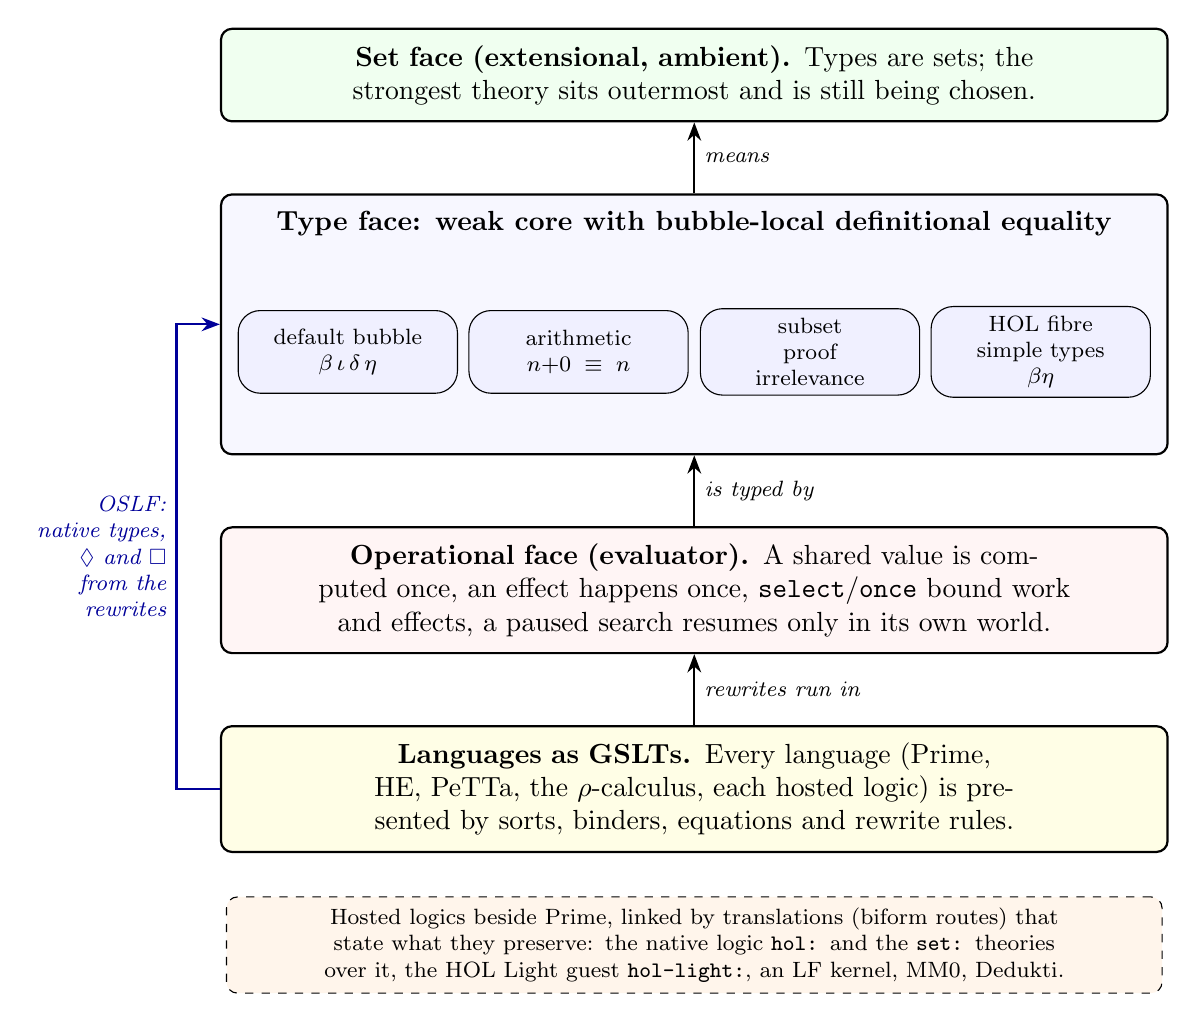
\begin{tikzpicture}[
  face/.style={draw, rounded corners, thick, align=center, inner sep=6pt},
  bub/.style={draw, rounded corners=8pt, fill=blue!6, align=center,
    font=\footnotesize, minimum height=1.05cm, text width=2.55cm},
  guest/.style={draw, dashed, rounded corners, fill=orange!8, align=center,
    font=\footnotesize, inner sep=4pt},
  lab/.style={font=\footnotesize\itshape}]
\node[face, fill=green!6, text width=11.6cm] (set) {%
  \textbf{Set face (extensional, ambient).} Types are sets; the strongest
  theory sits outermost and is still being chosen.};
\node[face, fill=blue!3, text width=11.6cm, below=0.9cm of set, minimum height=3.3cm,
  label={[anchor=north, yshift=-3pt]north:\textbf{Type face: weak core with
  bubble-local definitional equality}}] (type) {};
\node[bub] (b1) at ($(type.center)+(-4.4,-0.35)$) {default bubble\\
  $\beta\,\iota\,\delta\,\eta$};
\node[bub] (b2) at ($(type.center)+(-1.47,-0.35)$) {arithmetic\\
  $n{+}0 \equiv n$};
\node[bub] (b3) at ($(type.center)+(1.47,-0.35)$) {subset\\
  proof\\irrelevance};
\node[bub] (b4) at ($(type.center)+(4.4,-0.35)$) {HOL fibre\\
  simple types\\$\beta\eta$};
\node[face, fill=red!4, text width=11.6cm, below=0.9cm of type] (ops) {%
  \textbf{Operational face (evaluator).} A shared value is computed once,
  an effect happens once, \code{select}/\code{once} bound work and effects,
  a paused search resumes only in its own world.};
\draw[-{Stealth}, thick] (type.north) -- node[lab, right] {means} (set.south);
\draw[-{Stealth}, thick] (ops.north) -- node[lab, right] {is typed by} (type.south);
\node[face, fill=yellow!10, text width=11.6cm, below=0.9cm of ops] (gslt) {%
  \textbf{Languages as GSLTs.} Every language (Prime, HE, PeTTa, the
  $\rho$-calculus, each hosted logic) is presented by sorts, binders,
  equations and rewrite rules.};
\draw[-{Stealth}, thick] (gslt.north) -- node[lab, right] {rewrites run in}
  (ops.south);
\draw[-{Stealth}, thick, blue!60!black] (gslt.west) -- ++(-0.55,0)
  |- node[lab, pos=0.25, left, align=right, text=blue!60!black]
  {OSLF:\\native types,\\$\Diamond$ and $\Box$\\from the\\rewrites} (type.west);
\node[guest, below=0.55cm of gslt, text width=11.6cm] (g) {%
  Hosted logics beside Prime, linked by translations (biform routes) that state
  what they preserve: the native logic \code{hol:} and the \code{set:}
  theories over it, the HOL Light guest \code{hol-light:}, an LF kernel, MM0,
  Dedukti.};
\end{tikzpicture}
\caption{The three faces, the bubbles of the type face, and the hosted logics.
Every language is presented as a GSLT: its rewrites run in the operational
face, and from them OSLF derives native types and a modal logic in the type
face. Every
decidable or cheap fragment is a bubble carved inside the type face, and its good
properties are theorems about that bubble.}
\label{fig:prime-overview}
\end{figure}

{\small
\begin{longtable}{>{\raggedright\arraybackslash}p{2.3cm}
  >{\raggedright\arraybackslash}p{5.9cm}
  >{\raggedright\arraybackslash}p{2.3cm}
  >{\raggedright\arraybackslash}p{2.5cm}}
\toprule
Part & What is known & Status & PLN STV / ITV\\
\midrule
\endhead
Three faces & Every construct has a set face (meaning), a type face (checking)
  and an operational face (running), with links between them. & Decided &
  $\mathrm{STV}\langle 1.00, 0.92\rangle$ $[0.92,1.00]$\\
Sets ambient & A type is a set; the extensional side is the strongest.
  Membership is not yet connected to typing in the draft runtime. & Decided;
  realization open & Doc $\langle 0.95, 0.90\rangle$; Real $\langle 0.42, 0.86\rangle$ $[0.28,0.64]$\\
Identity & $J$ with $\iota$ in the core; no global K or UIP (``sans-K''); K
  and proof irrelevance in admitted per-space \code{(id:profile ...)} bubbles;
  UIP definable inside a non-UIP spine. & Decided &
  Doc $\langle 1.00, 0.92\rangle$; Real $\langle 0.89, 0.90\rangle$ $[0.80,0.95]$\\
$\eta$ & Kept, and type-directed; proof-producing $\beta\eta$ conversion
  recipes (\leanname{ConversionRecipes}) retain HOL equality witnesses. & Decided &
  Doc $\langle 1.00, 0.91\rangle$; Real $\langle 0.88, 0.89\rangle$ $[0.79,0.95]$\\
HE's type engine & Prime never falls back to it; HE-style fragments are decided
  by the hosted HOL Light checker. & Decided &
  Doc $\langle 1.00, 0.94\rangle$; Real $\langle 0.95, 0.90\rangle$ $[0.86,0.99]$\\
Candidate web & Prime is a web of explicit DTT candidates
  (\leanname{ParameterizedPiSigmaId}, \leanname{CumulativePiSigmaId},
  \leanname{StagedScopedReflective}) and carved profile bubbles (Lean, Agda,
  Rocq), never one monolithic calculus. & Decided &
  Doc $\langle 1.00, 0.93\rangle$; Real $\langle 0.82, 0.89\rangle$ $[0.71,0.91]$\\
Grounding \& 3 kernels & Tier-0 grounding is correct-by-construction (Rung~1:
  minimal HOL proves the checker faithful once); certificates and per-proof
  exports to HOL Light, Megalodon and MM0 are interop/acceleration bridges, all
  checking the same fiber semantics. & Decided &
  Doc $\langle 1.00, 0.92\rangle$; Real $\langle 0.71, 0.88\rangle$ $[0.56,0.84]$\\
Variables modulo $E$ & Repeated pattern variables denote equality of model
  elements modulo the active equational theory $E$ (presentation invariance;
  syntactic unification is the $E = \emptyset$ bubble). & Decided &
  Doc $\langle 1.00, 0.91\rangle$; Real $\langle 0.81, 0.89\rangle$ $[0.69,0.90]$\\
Least bubbles \& Horn fiber & Least sufficient bubbles do not exist in general
  (\leanname{no_least_sufficient_bubble}); a least bubble above every seed
  exists iff sufficiency is meet-closed (\leanname{tfae_mooreFamily}), for
  which Horn is the canonical finitary syntax (\leanname{models_hornTheoryOf},
  \leanname{oneStep_rulesOf}). & Decided; proved &
  Doc $\langle 1.00, 0.92\rangle$; Real $\langle 0.95, 0.90\rangle$ $[0.86,0.99]$\\
Normal-form fiber & Normalizing both sides and comparing decides a bubble's
  conversion on a set exactly when the set is weakly normalizing with unique
  normal forms (\leanname{decidedOn_iff_uniqueNormalForms}); for orthogonal
  theories of the $\lambda\Pi$-calculus modulo, exactly where they normalize.
  Outside: choice, identified variables ($\eta$ on variables, proof
  irrelevance), and commutativity on variables, for every theory
  (\leanname{not_decidedOn_of_commutative}). & Proved; end to end for HOL through Holide and STTfa; STTfa adequate over HOL proofs for normal coded terms; normalization of the typed hub and of other translations open &
  $\mathrm{STV}\langle 0.93, 0.88\rangle$ $[0.82,0.94]$\\
Inductive spine & Authored inductives join indexed polynomial containers
  $P = \Sigma_t \Pi_p \Delta_s$ (\leanname{IndexedPolynomial}) and
  representation-independent CeTTa backends (GMP exact integers) with
  proof-relevant $\iota$ policies (\leanname{ConversionRecipes.Policy}). &
  Decided; slice in progress &
  Doc $\langle 0.94, 0.89\rangle$; Real $\langle 0.67, 0.88\rangle$ $[0.52,0.80]$\\
GSLT and OSLF & Every language is presented as a GSLT (sorts, binders,
  equations, rewrites); OSLF derives its native types, predicates on terms with
  $\Diamond$ and $\Box$ from the rewrite relation. Binding signatures are free
  monads of context-indexed polynomial functors; collections as quotients are
  proved for single languages, with the general case in progress. &
  Proved pieces; design & $\mathrm{STV}\langle 0.80, 0.88\rangle$ $[0.67,0.90]$\\
Hosting & Three layers with their own crossing contracts: conversion bubbles,
  different logics, operational regions. A host preserves the counterexamples
  of its guest and declares what it adds. & Decided &
  Doc $\langle 1.00, 0.92\rangle$; Real $\langle 0.82, 0.89\rangle$ $[0.71,0.91]$\\
Kernel shape & A weak core (syntax-directed dependent typing with identity
  evidence) and bubbles that declare their conversion, each step justified by
  a global proof. Soundness, widening, substitution and the weakness order are
  proved; the version for full models of type theory and the decidability of
  joins of bubbles are open. & Proved core; design recommendation &
  $\mathrm{STV}\langle 0.84, 0.90\rangle$ $[0.73,0.93]$\\
Equality per bubble & Contextual by default: a paused read-only search that
  resumes only in its own world cannot tell contextually equal programs apart.
  & Proved for read-only searches; recommendation &
  $\mathrm{STV}\langle 0.80, 0.88\rangle$ $[0.67,0.90]$\\
Propositions & In a set model an impredicative universe is
  proof-irrelevant, so impredicative propositions are truth values and
  proof-relevant propositions are predicative types; irrelevance is an opt-in
  bubble. & Proved obstruction; recommendation &
  $\mathrm{STV}\langle 0.69, 0.87\rangle$ $[0.53,0.82]$\\
The top & The kernel's universe rules do not depend on the set profile; the
  top supplies universes as sets, at levels above $V_\omega$ exactly the
  $V_\kappa$ for inaccessible $\kappa$. Which set theory is outermost
  (hypersets are the stated direction) remains open. & Proved layering,
  conditional on cofinal inaccessibles; top open &
  Layer $\langle 0.80, 0.88\rangle$; Top $\langle 0.50, 0.86\rangle$ $[0.30,0.70]$\\
Operational contract & Twelve clauses: evaluation positions, binding,
  quotation, held data positions, shared and independent choice, ignored
  divergence, answer order, two kinds of effect, step/pause/resume, stale
  dependencies, \code{once} versus \code{select}. Function arguments are
  call-by-need by default while \code{let} is eager unless inside a \code{lazy}
  demand bubble. &
  Proved specification; runtime evidenced &
  Doc $\langle 1.00, 0.92\rangle$; Real $\langle 0.88, 0.89\rangle$ $[0.79,0.95]$\\
Execution contracts & Resource authority is reified to machine states;
  complete occurrence-query certificates compose through adaptive reads and
  validated resumption; dependent observer families share the existing
  preservation and erasure boundary. Resource-safe interleaving does not
  establish observable commutation, and permission weakening does not
  discharge a duty. & Proved abstract laws and query/control profiles;
  complete native instances open & $\mathrm{STV}\langle 0.82, 0.89\rangle$ $[0.71,0.91]$\\
HE types & Each fragment on which HE's checker is one well-defined typing
  relation (static arrows, schemes, tuples, meta-types, \code{\%Undefined\%} as
  the gradual unknown) is exactly typing in HOL, with three-way kernel agreement
  across HOL Light, Megalodon and MM0 (\leanname{KernelRealizations}). The named
  binders of the \code{he-prime} profile are genuinely dependent ($\lambda\Pi$). &
  Proved fragments \& 3-kernel agreement; dependent part open &
  $\mathrm{STV}\langle 0.84, 0.90\rangle$ $[0.73,0.93]$\\
Logic translations & The Grothendieck institution of a logic graph; borrowing
  a prover is sound exactly when the translation is conservative; proofs travel
  along routes. & Proved & $\mathrm{STV}\langle 0.85, 0.89\rangle$ $[0.74,0.93]$\\
HOL and sets & Classical HOL satisfies Farmer's seven virtues
  (\leanname{SevenVirtues}: Henkin completeness, Peano and COF categoricity,
  choice separation); intuitionistic HOL is complete for Heyting substitutional
  models (\leanname{HeytingGeneral}). Relativizing HOTG into its base logic is
  exact; HOL Light into HOTG and base into HOTG are not conservative. &
  Proved & $\mathrm{STV}\langle 0.91, 0.91\rangle$ $[0.82,0.97]$\\
Evidence logic & The four-valued reading of evidence (true, false, both,
  neither) is exactly double negation on the PLN evidence quantale. Counts
  summarize observations, and each operation is derived from a stated
  observation contract: additive revision for disjoint ledgers, an interval
  for overlap and for same-world conjunction, the paired product for pairs of
  sample bags, PLN's tensor for conditionally independent reports. Negation by
  evidence is monotone; PLN deduction is exact under screening off;
  conclusion confidence is derived through credal intervals. & Proved
  & $\mathrm{STV}\langle 0.90, 0.90\rangle$ $[0.80,0.96]$\\
Infinite MLNs \& DLR shells & DLR Gibbs completions induce additive world models
  (\leanname{MarkovLogicInfiniteWorldModel}); under the Dobrushin bound the query
  strength is fixed by the specification. The DLR query envelope has strict
  width exactly when the query observation leaks
  (\leanname{queryObservation_leaks_iff_strictWidth}); it collapses on the
  zero-weight grid and is strictly wide on the reinforced line. The IDM width of
  finite counts is a separate quantity (\leanname{EvidenceContracts.idm_width}).
  Extending a specification outside an interaction-closed core preserves the
  core's query strengths exactly (\leanname{TranscendencePath.original_queries_stable});
  agreement on an $n$-shell bounds the change by $2|\Gamma|C^n$ for some $C<1$
  (\leanname{DynamicTranscendenceStep.queryProb_approximately_preserved}).
  Reading these world models as bubbles is open and not yet investigated.
  & Proved; bubble reading open & Doc $\langle 0.95, 0.91\rangle$; Real $\langle 0.88, 0.89\rangle$ $[0.79,0.95]$\\
Weighted answers & One annotation semiring for spaces and answers; possibility
  composes exactly over positive semirings; commuting binds need commuting
  annotations; the answer readout is an observer of ordered runs. & Proved &
  $\mathrm{STV}\langle 0.85, 0.89\rangle$ $[0.74,0.93]$\\
Absence & Presence-only programs are coordination free; absence at a frontier
  is intuitionistic negation over reachable states, certified by the owner of
  the pattern's head and revoked only by it. & Proved; native source open &
  $\mathrm{STV}\langle 0.80, 0.88\rangle$ $[0.67,0.90]$\\
Choice, probability, strategy & Probability views a program with choice only
  through a scheduler, with envelopes at deterministic schedulers;
  consumption needs arbitration; bounded overtaking, realized by deadlines,
  certifies fair service. & Proved abstract laws &
  $\mathrm{STV}\langle 0.80, 0.88\rangle$ $[0.67,0.90]$\\
Empty and null & No universal null. Zero answers is not a value; an error is a
  value; an unknown call stays inert. Empty functions into different codomains
  are equal as sets and equivalent, not equal, as types. & Proved pieces;
  recommendation & $\mathrm{STV}\langle 0.80, 0.88\rangle$ $[0.67,0.90]$\\
Names & ``Bubble type theory'', glossed as a weak dependent type theory with
  bubble-local definitional equality (``fibered type theory'' also fits). The
  native logic is \code{(hol:profile base)}; the HOTG set theory is the set
  profile \code{(set:profile megalodon-hotg)}, built over that logic. & Decided
  & Doc $\langle 1.00, 0.90\rangle$; Real $\langle 0.94, 0.89\rangle$ $[0.84,0.99]$\\
\bottomrule
\end{longtable}
}

The weakest parts are the choice of the outermost set/hyperset theory, the
generic dependent eliminator derivation across the authored inductive spine, and
the Kripke--Henkin scheduler extension for intuitionistic HOL. The strongest are
the identity and $\eta$ decisions, the meet-closed (Horn) characterization of
least sufficient bubbles, Farmer's seven virtues for HOL, and the theorems that
make bubbles and hosting precise.

\section{The semantic envelope}

\subsection{The dependent total space is primary}

Suppose an operation begins in state $s$, receives a response $r$, produces an
outcome $a$, follows an occurrence-bearing route $\rho$, and incurs cost $k$.
The lossless semantic object is not merely $a$ but a dependent total space such
as
\[
  \mathcal{E}(s)
  = \sum_{r:R(s)}\sum_{a:A(s,r)}
    \sum_{\rho:\mathsf{Route}(s,r,a)} \mathsf{Receipt}(s,r,a,\rho)
      \times K.
\]
The response may select the result fibre.  The route, receipt, revision, owner,
and cost may be irrelevant to one observer and essential to another.  Therefore
none is definitionally reconstructed from the visible endpoint.

An observer is a map $q:\mathcal{E}(s)\to O$.  A dependent family
$B:\mathcal{E}(s)\to\mathcal{U}$ descends through $q$ precisely when it is
constant, up to the selected equality notion, on every fibre of $q$:
\[
  q(x)=q(y) \quad\Longrightarrow\quad B(x)\simeq B(y).
\]
This is the master non-collapse law.  It governs history erasure, extensional
typing, quotation, memoization, cost erasure, and coalgebraic quotienting.

\begin{proposition}[Observer licensing]
An extensional readout may forget a coordinate of the dependent total space only
when every consumer transported across that readout is invariant on the forgotten
fibres.  Endpoint equality alone is insufficient.
\end{proposition}

The current formal theory contains positive factorization theorems for
outcome-only continuations and negative canaries for history-sensitive families,
independent costs, and erased routes.  These results support an
\emph{intensional core plus licensed observers}; they do not yet select a concrete
rule package.

\subsection{Dependent and simple typing}

The simple/extensional face should be a fragment or observation of the dependent
face, not its replacement.  Andrews-style simple type theory is the default
mathematical and automated-reasoning waist when a notion is only a predicate
$P:A\to\mathsf{Prop}$ and all conclusions are insensitive to the particular
proof of $P(a)$ \cite{AndrewsTypeTheory,AndrewsAutomatingHOL}.  Reifying the notion as the subtype
$\{a:A\mid P(a)\}$ preserves existential and guarded-universal truth exactly;
the same construction works for a predicate on a genuinely indexed carrier by
using a dependent sum.  This accounts for weak noun-like types in controlled
mathematical language without promoting every guard to a new primitive type.

Constant families embed simple types into dependent types.  Genuine dependency
earns its cost precisely when a response, event, or proof selects the type of a
later object, or when a consumer distinguishes inhabitants of the selected
evidence fibre.  Propositionally truncating a two-inhabitant evidence fibre to
mere nonemptiness has no retraction, and a well-formed varying family exists
outside the constant-family image.  These are checked boundaries, not an appeal
to expressiveness by slogan.  Extensionality is orthogonal to simplicity: a
dependent theory can admit extensional observations, and a simple theory need
not identify all operational histories.

This boundary is internalized as a two-point capability order.  Simple typing
is the least sufficient profile for every literal constant family, while the
dependent profile is the least sufficient one for a checked varying Boolean
family.  This semantic choice is separate from choosing the strongest licensed
native implementation: first identify profiles that fully express the
consumer's required semantics and prefer weaker sufficient assumptions;
then choose a request-appropriate licensed native realization. A greatest
capability profile need not exist, and greater capability is not a theorem
of better runtime performance.

The current high-confidence intensional envelope contains contextual
substitution, $\Pi$, $\Sigma$, identity with $J$, and cumulative predicative
Tarski universes.  The remaining choice is between concrete rule packages,
conversion algorithms, universe mechanisms, and scoped equality principles.
No generic envelope theorem can make that choice on their behalf.  Following
Martin-L\"of's judgmental discipline, the shared identity capability must include
formation, reflexivity, dependent elimination, its reflexivity computation rule,
and stability of that computation under substitution \cite{MartinLofITT}.  A
native tower specimen now validates this complete contract with proof-relevant
computation receipts.  Neither global uniqueness of identity proofs nor equality
reflection follows from the contract; those remain separately licensed profile
properties.

\subsection{Kernel selection and generation requirements}
\label{sec:kernel-generation-requirements}

The following are maintained design requirements, not additional axioms or a
claim that a general kernel generator has been constructed. They distinguish
the logical commitments of a development, the capabilities available in a
native kernel, the trusted implementation, and the cost of using it.

\begin{description}[leftmargin=1.2cm,style=nextline]
\item[KG1: Semantic coverage.]
  A request states its required judgments, computation and equality laws,
  dependent data, observations, and universe bounds independently of the
  selected implementation. A configuration is sufficient only through the
  corresponding interpretation and adequacy obligations. Syntax coverage,
  a capability label, or soundness alone does not establish full coverage.
  Required distinctions must be reflected or retained by a checked decoding;
  a quotient is permitted only when licensed by the request. No selection may
  silently weaken that request. Expressibility does not entail a total decision
  procedure for theoremhood or program behavior.
\item[KG2: Minimal logical commitments.]
  Prefer the weakest sufficient object theory and equality/universe profile
  within the stated comparison class. Report the assumptions actually used
  by a development separately from those available in its ambient kernel.
  Where no least profile is established, retain incomparable minimal
  candidates rather than inventing a total strength ranking. Access to a
  stronger kernel does not by itself justify stronger object-theory assumptions.
  A local development can therefore work in ZF and explicitly acquire choice
  when needed, even if its host also offers stronger set or type theories.
  Returning to the weaker context requires accounting for the proof and the
  declarations it used, not merely recognizing its conclusion's vocabulary.
  Proof-local dependency reduction and weakening an object theory's model
  class are separate obligations: deleting an authored axiom does not remove
  the same law if the chosen model interface still requires it.
\item[KG3: Appropriate native capabilities.]
  Among configurations meeting the semantic and trust requirements, select,
  host, compose, or specialize native decision, proof, operation, and external
  certificate services as appropriate. An efficiently implemented derived rule
  may increase native capability without increasing logical strength; its
  admissibility or conservative-extension obligation must be proved.
  Certificate replay is one service boundary, not the definition of NIK.
\item[KG4: Checked kernel generation.]
  Generate feature-selected kernels and their implementations from admitted
  presentations and explicit feature-interaction laws. Their operational stages
  remain GSLTs; an implementation has an independently justified relation to
  that operational meaning. The generated artifact must be bound to the
  selected semantics and profile, with separate source-to-artifact and
  artifact-execution obligations. Generation does not certify itself, and
  correctness of individual features does not establish correctness of every
  combination. The chosen trust boundary and bootstrap remain explicit.
  Generation and specialization may be demand-driven: feature materialization
  can be deferred until needed. Admission may not be deferred past trusted use,
  nor may a newly supplied feature silently alter an earlier judgment's
  meaning. Cached results require the qualified dependencies of KG6.
  Formation, preservation of conversion classes, preservation of assigned
  types, and termination of an unfolding strategy are distinct obligations.
  A proof of one may not stand in for another; total conversion decision
  needs its own justified scope even for transparent definitions.
  Local computation admission must support a contextual preservation theorem,
  including transport of binder assumptions and dependent result types.
  Checking selected redex/reduct endpoints alone does not establish that law.
  A declaration/computation restriction that retains a proof and reflects
  admitted judgments is not thereby an independently qualified evaluator.
  Its retained rules must also retain the declaration and schema dependencies
  needed by their reducts, and satisfy the restricted package's preservation
  and conversion contracts. Proof replay and executing-kernel specialization
  are different services.
  Recovering a rule's typed parameters from an observed application is an
  explicit obligation. A named declaration can supply a principal spine;
  arbitrary unannotated terms need not have unique types.
  Constructor-conversion safety need not be proved by confluence of the
  authored runtime reduction. A proof-only completion is permitted when its
  conversion theory is proved identical and its joining argument retains the
  required constructors. Its extra proof steps are not executable rules or a
  conversion decision procedure without separate justification.
  Finite conversion-evidence checking is a separate service contract:
  accepted codes must imply the selected conversion relation, and any claimed
  evidence completeness must cover that relation rather than only reflexivity.
  Termination on a supplied code does not imply a terminating search for one.
  Rejecting a particular code is not a proof that its endpoints differ.
\item[KG5: End-to-end efficiency.]
  Compare generation, specialization, execution, checking, translation,
  memory, and retained evidence costs without trading away KG1. Native rules
  and compact proof terms can avoid costly expansion into a smaller kernel.
  Conversely a smaller trusted implementation may be preferred when the
  workload and trust policy justify it. Neither logical strength, feature
  count, nor trusted-code size is a substitute for a proved or measured cost
  comparison; no universally optimal generator is assumed.
  For the planned CBPV basis, lazy/eager rewrites must preserve the selected
  termination, effect, sharing, occurrence and result observations before their
  costs are compared. A strategy change is not an unconditional equation.
  Keeping code as a value does not by itself memoize its outcome. A rewrite
  may qualify each actually selected suspended body while allowing effects in
  its selection and consumer. Eliminating a forwarding cell requires an
  explicitly coarser observation or a proved resource/receipt correspondence;
  equality of returned dependent pairs alone does not justify that erasure.
  Selecting an effectful service provider once and selecting it at each call
  can preserve acceptance support while changing proof artifacts, correlated
  choices, occurrences and intents. Function-space interfaces do not license
  moving that selection across application.
\item[KG6: Revisable qualification.]
  Bind each selection and generated artifact to a revision of its semantic
  requirements, feature assumptions, and dependencies. A revision needs
  justified transport or renewed admission; it cannot silently reinterpret an
  earlier artifact. Maintain positive and negative controls and distinguish
  proved, conditional, refuted, and open properties in the status ledger.
  For a fixed checker, a dependency manifest must include the lookup results
  actually protected by its contract, including absence, declaration
  transparency, and dependencies exposed by selected definitions or known
  propositions. An unchanged input name or type alone is not such a contract.
  A dependent cached reply must retain the full request that indexes its
  meaning, not only an equal result tag. A changed proof producer may leave
  an already checked proof usable at that unchanged request; a changed
  judgment or request needs independent transport or a new invocation.
  Rejecting a stale packet must not silently relabel it or refute the new
  mathematical proposition.
  A suspended producer's captured environment is distinct from its consumer
  continuation. Reusing a completed native value must neither rerun producer
  effects nor restore an earlier mutable-state snapshot. A retryable cache
  reset does not itself roll back already recorded effects; transactional
  behavior requires a separate contract.
\item[KG7: Reusable kernel components.]
  Reuse binding, substitution, declaration lookup, rule instantiation and
  checking components through explicit contracts. An extension must state
  whether it preserves old judgments, conversion, proof identity and model
  meanings, and which interactions require new proofs. Adding a set-theoretic
  object theory need not add a kernel inference rule; adding dependency changes
  the formation and substitution contract and is not merely another axiom list.
  Count the transitive trusted dependencies of a selected service, including
  its primitive operations, rather than only the size of its outer dispatcher.
  Reified computation bodies must preserve scoped binding under substitution.
  Native-value binders and suspension-reference binders must retain their
  distinct scopes. A replacement that carries variables of several sorts
  must be weakened along every binder sort it crosses. Scope and constructor
  conformance alone cannot rule out cross-sort capture: a captured reference
  can remain in bounds while naming a different cell. Returned values,
  computation functions, ordinary thunks and shared Need references must
  retain their distinct roles. Capturing a thunk stores lexical data, not
  a consumer world; caching its construction does not cache its executions.
  A local application or ordinary force must not invent an effect receipt
  or a sharing allocation to enter its captured code. Heap qualification
  relates each captured producer and cached answer to an independently
  declared cell type; lookup success alone is not mathematical admission.
  Whole-run admission must derive intermediate heap and continuation
  qualification from initial source typing and the primitive contracts,
  rather than assume those invariants anew at each observation. A commit
  retains its cell's declared type, while a consumer's result conversion
  retains its independent formation and conversion evidence.
  Fresh allocation must transport the captured environments inside cached
  functions as well as suspended producers. A returned executable closure
  remains coupled to its qualified final heap; an answer-only type projection
  is not a reusable closure environment. Allowed fault shapes must be
  distinguished from evidence about the event that produced a fault.
  Operation declaration formation, operational realization and preservation
  of the declared result family are distinct contracts. Agreement with an
  operation's own evaluator cannot replace the last contract.
  Source evaluation must also be stated independently of machine steps.
  Completed-outcome correspondence must retain the required heap, effects,
  choice occurrences and failure status, not just successful native values.
  Finite path existence does not establish result-list multiplicity, cost,
  termination or fairness; a bounded search with no answer is not a source
  refutation. Native admission remains conditional on the separately
  qualified source, environment, heap and primitive result contracts.
  A function consumer may execute a captured body and change the world.
  Its source interpretation must therefore retain an intermediate answer
  and world, not merely repackage a returned result. Final-heap qualification
  must concern that same world, not another execution with an equal answer.
  An execution equation must declare where substitution by that equation
  is licensed. Exact completed evaluation can be retained by an active
  consumer without being a congruence under quotation, source capture or
  allocation. Lexical body opening and source-term substitution are distinct
  operations when returned closures retain their source environments.
  An immediate-demand rewrite must respect the producer's computation
  polarity; its type qualification cannot be inferred from one successful run.
  A semantic value/computation adjunction must identify its induced sequencing
  with the existing computation operations. This alone does not supply all
  computation type formers or reified source substitution. Delayed native
  service data, its independent result-family qualification and any stored
  admission evidence remain separate; erasure compatibility does not recover
  proofs from unqualified raw execution.
  A raw mathematical-service reply must retain the exact request and article
  without assuming its own checker verdict. Data formation, structural
  decoding, selected-calculus checking and logical interpretation are
  separate obligations. A copied acceptance tag has no authority; scope
  labels require an independently fixed association with the selected
  calculus. Rechecking an untrusted reply and reusing authenticated evidence
  are different execution contracts, with different costs.
  A first-class checker retains that contract when passed through a caller;
  its function type alone cannot authenticate arbitrary checking code.
  Sharing a provider selection, sharing a returned reply and caching the
  provider's individual applications are different transformations.
  An executable proof materializer must reconstruct the submitted tree,
  interpret its actual rules and separately qualify the resulting native
  term; returning a well-formed data marker does none of these.
  A native extension must qualify the exact combined rule package, not borrow
  a conversion boundary from a smaller one. Declaration formation, primitive
  preservation and conversion safety are separate obligations. A proof-only
  completion may establish the last while its executable checker continues
  to recognize only the original rules. Checking a reduction cannot replace
  independent admission of its source.
  A richer computation-object interface must preserve the existing free
  programs and supply its contextual universal properties. A terminal
  computation algebra is not an effectful program returning a singleton;
  interpreting in the former does not justify discarding the latter's work.
\item[KG8: Integrated mathematical entry.]
  CeTTa is the metaprogramming home for mathematical construction, search,
  checking, and proof use. Its ordinary programs must be able to manipulate
  and invoke the same qualified mathematical services as an interactive client.
  Pure theorem development and verification must be able to use native NIK
  services without first acquiring a programming-language evaluation semantics.
  The direct ITP interface is a shared component boundary, not a requirement
  for a separate mathematical product. Proof search and elaboration remain distinct
  from their admitted judgments. A service's own operational implementation
  still requires its GSLT presentation and realization; this does not turn
  the mathematical object theory into the client's programming language.
\item[KG9: Homoiconic integration with qualified elaboration.]
  Higher-order, dependent-type and set-theoretic constructions should remain
  ordinary inspectable program data, with scoped vocabulary such as
  \nolinkurl{lang:}, \nolinkurl{type:}, and \nolinkurl{set:} rather than an
  undifferentiated top-level namespace. These names organize access; they do
  not identify three foundations or erase the distinction between a framework
  and an object theory. Elaboration may infer parameters, insert admitted
  translations, and obtain reusable checking evidence automatically. The
  elaborated terms, selected theory and revision, inserted maps, remaining
  obligations and trust dependencies must remain inspectable. Automatic
  handling cannot promote unresolved work to proof, discard required evidence,
  choose an ambiguous meaning silently, or identify distinct conversion laws.
  Each insertion requires the appropriate substitution, meaning-preservation
  and required-reflection laws; a common surface notation is not such a proof.
  A local abstraction scope also names its observation and equality discipline.
  Changing scopes may insert a checked transport or forget declared distinctions;
  it must not turn observational agreement or temporal lineage into intensional
  identity. Ordinary reasoning within a scope should not require manually
  repeating these qualifications at every use.
\end{description}

Current evidence covers parts of this contract: the two-profile
\nolinkurl{SimpleDependentCapabilitySelection} proves least sufficiency for
constant and genuinely varying family specimens, not for arbitrary calculi;
\nolinkurl{CapabilitySelection} selects within a finite licensed family for
a fixed semantic request; \nolinkurl{SemanticService.Service} keeps all four native-service
faces; and \nolinkurl{MachineCompilationCorrectness} separates compilation provenance
from execution refinement on its checker-facing boundary. These results do
not yet synthesize arbitrary feature combinations, decide semantic sufficiency
in general, or provide a universally weakest or fastest kernel.
The equality specialization specimen supplies a further instance of KG3:
a native generic definition and reflexivity proof are reused at every closed
plain type, with source-level formation and checking proved independently.
Its comparison with intrinsic extensional equality exposes an explicit model
condition rather than importing set axioms or dependency. This is checked
specialization of one native feature, not a feature-combining kernel generator.
Checked definition expansion supplies another local instance: partial
constant-to-term substitution preserves successful results when its available
replacement table is extended. Native unfolding agrees exactly with its typed
interpretation at each fuel bound, and additional fuel preserves a successful
result. Type preservation, semantic definition equations, and termination are
separate obligations. These facts support demand-driven specialization; they
do not establish incremental kernel generation or an end-to-end speedup.
Exact environment-local reuse is now proved for the existing Lean implementation
of native Megalodon checking, separately from its partial Henkin interpretation. A finite manifest
containing the input dependencies, closed under selected definition bodies and
known propositions, and preserving the selected lookup results gives exactly
the same proof-checking verdict at every unchanged fuel bound. Executable
manifest checks discharge these premises. This is a sufficient frame criterion,
not a minimal-dependency theorem or logical conservativity of arbitrary added
axioms. It applies to revisions of the environment of this fixed checker;
changing its inference or conversion rules requires a separate extension proof.

The modular theory $\mathcal U$ of Blanqui et al. provides a particularly close
precedent for KG2 and KG7 \cite{BlanquiModularTypeTheories}. Its fragment theorem
recovers a derivation in a subtheory when the context, proof and conclusion
belong to that fragment. The fragment must be closed under declaration-type
dependencies and all ambient rewrite rules whose left sides it contains;
confluence and type preservation are substantive conditions. This is not the
claim that every theorem stated in the smaller language has a proof there.
Bauer and Petkovi\'c Komel supply a complementary reusable equality algorithm
for user-defined type theories, separating computation and extensionality rules
\cite{BauerPetkovicEquality}. Their soundness result does not supply termination
or completeness for every feature selection. Together these works motivate
dependency-sensitive proof reuse and separately qualified conversion components,
not automatic compatibility of arbitrary kernel features.

The candidate \nolinkurl{PrimeCandidates.EntryModeSelection.nativeProofOperation}
supplies a claim/native-proof service interface independent of a
programming-language run. Its comparison with replay uses two interfaces to
the same guest kernel, not independent physical implementations. A direct
interactive client remains to be implemented. Likewise, coGSLT-authored
judgment and inference extensions provide additional mathematical input:
\nolinkurl{ConservativeExtension.extension_not_determined_by_core} refutes
recovering all extension declarations from the core alone. A generator must
consume such input and its laws; it cannot infer an arbitrary proof calculus
from an operational language or a list of desired properties alone.

Small trace interfaces illustrate the same distinction. The MM2 execution
description delegates matching and emission to sources and sinks, whose
available operations include state changes and foreign computation
\cite{MORKMM2,MORKSourcesSinks}. Moving execution into a sink moves its semantic
and implementation obligations rather than eliminating them. The local MM21
sink-scheduling proposal is still an open specification question, not a proved
two-rule verifier. The existing NIK finite-trace construction requires a sound
local edge authority, including any premise discharger for queries,
substitution, binders or capabilities. Finite edge checking does not establish
termination, fairness or validity of infinite executions.

\subsection{Quantitative observers without admission by similarity}
\label{sec:distinction-calculus}

The distinction calculus provides a quantitative companion to exact
observation contracts \cite{GoertzelDistinctionCalculus,GoertzelDistinctionClosure}.
Its similarity kernel is not a proof kernel. The checked rational fragment
in \nolinkurl{Cybernetics.DistinctionCalculus} starts with a symmetric,
reflexive matrix $\alpha:X^2\to\mathbb{Q}\cap[0,1]$, without assuming
transitivity. Its complementary distance is $d_\alpha=1-\alpha$.
The paper's metric condition is a triangle law; separation is not assumed,
so this is a pseudometric. Positive distance implies distinct states, but
distinct states need not have positive distance under a lossy observer.
Triangle coherence supplies cotransitivity of positive apartness and a
setoid of zero-distance states. A goal descends to the resulting quotient
exactly when it is invariant on its zero-distance classes; the construction
reuses \nolinkurl{Cybernetics.MultiscaleGoal}.

Raw certificates derive upper distance bounds by authored edges,
reflexivity, the unit bound, symmetry, capped triangle composition and
weakening. The total checker agrees with a separately defined derivation
relation. Its semantic theorem ranges over every metric similarity extending
the seed, a nonempty model class. In particular,
\[
\alpha\vdash_{\mathrm{completion}} d(x,z)\leq
\min\{1,d_\alpha(x,y)+d_\alpha(y,z)\}
\]
does not assert this bound in an incoherent seed. A finite proposed
completion is admitted only after checking its observer laws, metric
coherence, extension of the seed, and a path certificate for each proposed
distance. \nolinkurl{completionCheck_sound} proves that an accepted
candidate is the \emph{least} metric extension, not merely a feasible
matrix. No particular shortest-path generator is trusted by this result.
The graded control derives similarity $3/5$ from adjacent similarities
$4/5$; an endpoint-collapse certificate is impossible. In the crisp
three-node chain, completion really does identify previously distinguished
endpoints, reducing uniform distinction from $2/9$ to zero.

For a rational probability weight $\mu$, the checked bracket is
$g_\alpha=\sum_{x,y}\mu_x\mu_y\alpha(x,y)$, with distinction
$h_\alpha=1-g_\alpha$. Migration distortion compares the declared source
and transported target similarities. Zero distortion implies equality of
those similarities on supported pairs; the global equivalence theorem
requires full support. Route composition obeys a triangle bound under the
same source pair law, and a balance theorem separates state change from
observer change. These scores do not replace exact consumer compatibility.

\nolinkurl{PolarizedNeedDistinctionObserver} instantiates this distinction
on the executed Lean reference workload of a shared versus freshly selected
inference provider. Every completed branch retains the same two native
replies, but event frontiers distinguish the programs. Erasing those events
has distortion $1/2$ on the explicitly uniform two-program population,
not a probability measure on runtime branches. A second result proves
that actual article-admission verdicts cannot factor through the requested
theorem alone: one article is accepted and another for the same request is
rejected. Neither result authorizes replacing Need sharing by unshared
evaluation or establishes a C implementation correspondence.

This supplies a precise application of observer-relative multiscale goals
\cite{FieldsLevinCompetency}. It does not identify biological agency with
a quotient construction. In particular, observation coverage is not
beneficence: a finite control gives equal distortion but opposite signed
changes of a separately declared goal value. Structure-preserving repair
likewise retains its value and misfit obligations; similarity alone cannot
discharge them. Futamura specialization and Turchin supercompilation
\cite{FutamuraRevisited,TurchinSupercompiler} suggest producers for
specialized checkers and transformations. Their semantic correspondence,
termination, preservation of sharing and resource benefit remain separate
requirements, not consequences of low distortion.

\subsection{Evidence: observation contracts, readouts and PLN}
\label{sec:evidence-contracts}

A pair of counts $(n^+,n^-)$ summarizes observations: how many samples
supported a proposition and how many refuted it.  Which operations on such
pairs are sound depends on what was observed and how the observations
relate.  The checked development states the relation as an
\emph{observation contract} and derives each operation from it; no
combination formula is postulated.  Probability is read from evidence; the
evidence is what a world model carries.

\paragraph{Identified observations.}
When every observation has an identity, a body of evidence is a ledger, a
finite set of identities, each recording one world.  Ledgers form a
distributive lattice whose join is union: merging two replicas is idempotent,
commutative and associative, so ledgers replicate without coordination.  The
evidence of a ledger is a valuation on that lattice: the evidence of a union
plus the evidence of the overlap is the sum of the two evidences
(\leanname{EvidenceContracts.ledgerEvidence_union_add_inter}).  Consequently
additive revision is exact exactly for disjoint ledgers and otherwise counts
the overlap twice (\leanname{additive_revision_exact_iff_disjoint},
\leanname{revision_counts_overlap_twice}); the disjointness check that
non-axiomatic reasoning performs on evidential bases before revising
\cite{WangNAL} is this condition.  Retraction of a ledger subtracts the
evidence of its overlap by the monus of counts (\leanname{ledgerEvidence_sdiff}),
and the abstract overlap world model of the tree is instantiated with the
overlap read off the intersection (\leanname{ledgerOverlapModel}).  When the
overlap is unknown, the merged evidence lies between the coordinatewise
maximum and the sum of the two evidences, and both ends occur for the same two
evidences (\leanname{unknown_overlap_bounds},
\leanname{Controls.overlap_interval_ends}).  The maximum is therefore the
revision that is sound whatever the overlap, the counting analogue of
covariance intersection \cite{JulierUhlmannCI}.  The source-keyed revision of
the layer atlas, which keeps each source's cumulative evidence and merges by
maximum, computes the evidence of the merged ledger exactly when each
source's observations on the two replicas are nested, as under cumulative
publication, and under-counts otherwise
(\leanname{ledgerEvidence_union_eq_sourceMerge},
\leanname{Controls.sourceMerge_undercounts}).

\paragraph{Pairs of samples and the weights of answers.}
Pairing every sample of one bag with every sample of another forces the
paired product $(a^+b^+,\;a^+b^-+a^-b^++a^-b^-)$
(\leanname{EvidenceSpaces.conjunction_unique}); in the coordinates (positive,
total) of non-axiomatic logic it is coordinatewise multiplication
(\leanname{EvidenceSpaces.posHom}, \leanname{EvidenceSpaces.totalHom}), and its
strength is the product of the strengths.  With it the counts form a
commutative semiring, so evidence can weight answers.  Which laws of an
annotation semiring a readout needs is now exact.  Possibility composes for
all answers if and only if the semiring is \emph{positive}: sums vanish only
when both summands do and products only when a factor does
(\leanname{AnnotationCapabilities.support_bind_iff_positive}); this is
equivalent to a zero-reflecting homomorphism into the two-element semiring
(\leanname{positive_iff_exists_hom}), as in the semiring provenance of
first-order logic \cite{GradelTannenProvenance}.  Evidence counts with the
paired product are positive, the coordinatewise product on pairs is not, and
no nontrivial ring is (\leanname{positive_evidence},
\leanname{not_positive_pair}, \leanname{not_positive_of_ring}): signed
weights retract anything exactly but lose compositional possibility, while
the monus retracts only a known batch and keeps it.  Two independent binds
commute for all answers only if the annotations commute
(\leanname{comm_of_bind_comm}).

The total of a paired product counts pairs, not independent samples of the
conjunction.  For independent bags of sizes $n$ and $m$ with success
probabilities $p$ and $q$, the variance of the number of positive pairs is
\[
  nm\,pq(1-pq)\;+\;nm\,pq\bigl((m-1)q(1-p)+(n-1)p(1-q)\bigr),
\]
derived from the sampling model by finite sums
(\leanname{PairedSampleDispersion.paired_variance}).  The first term is the
variance for $nm$ independent joint samples; the excess vanishes for interior
probabilities exactly when $n=m=1$
(\leanname{paired_variance_eq_joint_iff}).  At $p=q=1/2$ the effective number
of independent joint samples is $3n^2/(2n+1)$, below $3n/2$, not $n^2$
(\leanname{Controls.effective_size_half}).  A confidence readout for a
conjunction must therefore be derived from the factors' counts and strengths,
not from the paired total.

\paragraph{Observations of one world.}
Two predicates evaluated on the same bag of worlds have marginal counts that
do not determine their conjunction
(\leanname{EvidenceSpaces.no_same_world_conjunction_from_marginals}).  The
compatible conjunction counts are exactly the Fréchet interval
$\max(0,a+b-n)\le c\le\min(a,b)$ \cite{FrechetTableaux}: every value in it is
realized by a bag and none outside it
(\leanname{EvidenceContracts.conjunction_counts_iff}).  The product of the two
frequencies lies inside (\leanname{independence_within_frechet}).  For
dependent observations the sound readout of a conjunction is this interval;
independence is an assumption that selects one point.

\paragraph{Reports about one hypothesis.}
A report can instead be read as the pair of masses of a hypothesis and of its
negation jointly with the report.  For two reports conditionally independent
given the hypothesis, under a uniform prior, the evidence of both reports is
the coordinatewise product of the single-report evidences, up to the prior
constant, and its strength is the posterior probability
(\leanname{testimony_fuse_uniform}, \leanname{strength_fuse_uniform}).  This
coordinatewise product is PLN's binary-evidence tensor
(\leanname{toPaired_tensor}).  Its strength is the logarithmic opinion pool
\cite{GenestZidekPooling}, or Dempster's rule on Bayesian mass functions over a
two-element frame \cite{DempsterUpperLower} (\leanname{strength_fuse}); its
zero divisor is total conflict between two certain reports
(\leanname{fuse_total_conflict}); and fusing two posteriors that each contain a
non-uniform prior counts the prior twice
(\leanname{testimony_fuse_counts_prior_twice},
\leanname{Controls.prior_counted_twice}).  Likelihood ratios of independent
tests multiply in the same way as betting scores do in game-theoretic
statistics, where the product of independent e-values is an e-value
\cite{VovkWangEValues,ShaferVovkGTP}.  The tensor is thus a sound fusion
operator for its own contract.  It is not conjunction and not the direct path
of PLN deduction: on two half-strength premises it has strength $1/2$, while
the direct-path term $s_{AB}s_{BC}$ is $1/4$, the strength of the paired product
(\leanname{Controls.fuse_not_direct_path}).

\paragraph{Readouts.}
Strength is undetermined with no samples
(\leanname{EvidenceSpaces.readout_zero}), never strength zero.  The interval of
Walley's imprecise Dirichlet model \cite{WalleyBagOfMarbles} is $[0,1]$ at zero
counts (\leanname{idm_vacuous}); its width is one minus the PLN confidence
$n/(n+s)$ (\leanname{idm_width}), and with samples it contains the observed
frequency (\leanname{idm_contains_frequency}).  Revision shrinks the width but
moves the interval, so the intervals of successive evidence states are not
nested (\leanname{idm_not_nested}).  The vacuous interval coincides with the
probabilities that schedulers assign to a pure nondeterministic choice between
two outcomes (Section~\ref{sec:demand-effects}).  Strength is not additive
under revision (it is the mediant, \leanname{EvidenceSpaces.strength_add}), so
the weights of alternatives must be carried as counts and read out once.

\paragraph{Negation by evidence, not by absence.}
Evidence against a proposition is recorded, not inferred from a missing
record.  Exchanging the two counts is an involution that is monotone in the
information order and distributes over revision
(\leanname{against_mono}, \leanname{against_add}); the truth-order meet and join
of the evidence bilattice are monotone in the information order and exchanged
by it (\leanname{tmeet_mono}, \leanname{tjoin_mono}, \leanname{against_tmeet}); and
the four-valued reading as neither, true, false or both \cite{BelnapFourValued}
is monotone (\leanname{belnap_mono}).  This is the constructible falsity of
Nelson \cite{NelsonConstructibleFalsity}, which the basic logic of evidence of
Carnielli and Rodrigues reads as preservation of evidence
\cite{CarnielliRodriguesLET}: every connective only grows with evidence, so a
program built from them stays presence-only and coordination free.  The
intuitionistic negation $a\Rightarrow\bot$ of a nontrivial Heyting algebra is
not monotone (\leanname{hnot_not_monotone}), in particular on PLN's evidence
frame (\leanname{binaryEvidence_hnot_not_monotone}).  Negation by absence
therefore needs a frontier (Section~\ref{sec:pqi-absence}); negation by
evidence does not.

\paragraph{What PLN's rules become.}
Revision is derived for disjoint ledgers and refuted for overlapping ones.  The
strength of a conjunction is derived for independent sample bags and is only
an interval for observations of one world.  Inversion is Bayes' rule in counts
(\leanname{EvidenceSpaces.condition_pos_symm}).  Deduction is exact under
screening off: if, in the counts of a bag of worlds, $C$ is independent of $A$
given $B$ and given $\neg B$, the frequency of $C$ among the $A$-worlds is
$s_{AB}s_{BC}+(1-s_{AB})(p_C-p_Bs_{BC})/(1-p_B)$
(\leanname{EvidenceContracts.deduction_exact_of_screening}); without screening
off the formula gives $1/4$ where the frequency is $0$
(\leanname{Controls.deduction_fails_without_screening}).

\paragraph{Conclusion confidence through intervals.}
A conclusion's confidence is derived through credal intervals, in the sense of
the confidence characterization of the tree: a truth value $\langle s,c\rangle$
is a readout of a credal envelope.  The route has three steps.  Premise
evidence $(n^+,n^-)$ becomes the imprecise Dirichlet interval with a declared
prior strength $s$, an envelope theorem of the tree
(\leanname{WalleyBinaryIDM.credal_envelope_matches_Walley_ITV_bounds}); its
evidence weight reads back $n^++n^-$ (\leanname{EvidenceContracts.idm_intervalWeight}).
The rule then maps premise intervals to a conclusion interval by the map its
observation contract fixes: the product interval for independent pairs
(\leanname{product_interval}), the Fréchet interval for conjunction on one world
(\leanname{frechet_interval}), the corner interval of the bilinear deduction map
under screening off (\leanname{deduction_interval},
\leanname{bilinear_between_corners}), and the vacuous interval $[0,1]$ without
screening off, where two bags agree on $s_{AB}=s_{BC}=1/2$ and give $C$ among the
$A$-worlds the frequencies $0$ and $1$ (\leanname{Controls.unscreened_vacuous}).
Finally a declared selector gives the strength and the width-complement chart
the confidence, which is the PLN odds chart $w/(w+s)$ for the interval's
evidence weight $w$ (\leanname{widthConfidence_eq_odds}); the chart is forced by
the Walley gate (\leanname{walley_width_complement_forces_plnOdds}).
\leanname{deduction_confidence_route} assembles the steps for deduction.
\begin{center}
\small
\begin{tabular}{>{\raggedright\arraybackslash}p{0.27\linewidth}%
                >{\raggedright\arraybackslash}p{0.25\linewidth}%
                >{\raggedright\arraybackslash}p{0.38\linewidth}}
\toprule
Choice & Status & Fixed or justified by \\
\midrule
Prior strength $s$ ($\kappa$) & genuine degree of freedom & declared per context
  and source \\
Credal model of a premise & genuine backend choice & the imprecise Dirichlet
  model is the one whose width complement is the PLN chart \\
Range and normalization & convention & the declared range $[0,1]$ \\
Confidence chart & free until gated & forced to $w/(w+s)$ by the Walley gate \\
Propagation map & fixed & the observation contract of the rule \\
Strength selector & genuine decision knob & lower, midpoint, upper or point
  estimate; it does not affect confidence \\
Rule-level transport & computed in interval or weight space & raw-confidence
  transport double-damps: inputs $(0.5,0.5)$ give $0.5$ under minimum-support
  transport, not $0.333$ (\leanname{truthInduction_conf_eq_min_capped}) \\
\bottomrule
\end{tabular}
\end{center}
Against this route, the deduction evidence constructed in the tree, whose total
is the sum of the premise totals (\leanname{EvidenceContracts.deductionEvidence_total}),
is neither an upper nor a lower bound.  On premises $(1,1)$ and $(1,1)$ with
$s=1$ it posits $4$ (\leanname{Controls.deductionEvidence_posits_four}); the
route derives the interval $[1/9,4/9]$ and weight $2$ at $p_B=p_C=0$, and the
interval $[4/9,5/9]$ and weight $8$ at $p_B=p_C=1/2$; on premises $(0,2)$ and
$(1,2)$ at $p_B=p_C=0$ both give $5$ (\leanname{Controls.deduction_posited_overstates},
\leanname{Controls.deduction_posited_understates},
\leanname{Controls.deduction_posited_agrees}).  Likewise the weight-product
conjunction of the tree, $w_{a\wedge b}=w_aw_b$, gives confidence $4/5$ on
premises $(1,1)$ and $(1,1)$, where the route derives $2/3$ for independent
conjunction and $1/3$ for conjunction on one world
(\leanname{Controls.conjunction_through_intervals},
\leanname{Controls.frechet_through_intervals}); the weight product is the paired
total, which the variance identity above shows overstates.

\paragraph{Neighbouring formalisms.}
The same counts underlie several formalisms that read them differently.
\begin{center}
\small
\begin{tabular}{>{\raggedright\arraybackslash}p{0.21\linewidth}%
                >{\raggedright\arraybackslash}p{0.33\linewidth}%
                >{\raggedright\arraybackslash}p{0.36\linewidth}}
\toprule
Formalism & Its reading of $(n^+,n^-)$ & Relation to the contracts above \\
\midrule
Non-axiomatic logic \cite{WangNAL} & frequency $w^+/w$, confidence $w/(w+k)$ &
  revision adds evidence after a disjointness check of evidential bases: the
  ledger contract \\
Subjective logic \cite{JosangBeliefCalculus} & opinions in bijection with Beta
  evidence & cumulative fusion, for separate and independent evidence, adds the
  evidence parameters, and averaging fusion, for the same evidence, is
  idempotent \cite{JosangFission}: the ledger contract at its two ends; the
  product of opinions coarsens the product frame and approximates the exact
  product \cite{JosangBeliefCalculus} \\
Dempster--Shafer \cite{ShaferEvidence} & mass on hypotheses and on the frame &
  Dempster's rule on Bayesian masses is the likelihood contract, and total
  conflict is its zero divisor \\
Imprecise probability \cite{WalleyBagOfMarbles} & credal sets &
  the imprecise Dirichlet interval, vacuous at zero counts \\
Game-theoretic probability \cite{ShaferVovkGTP} & betting capital &
  independent betting scores multiply: the likelihood contract \\
Semiring provenance \cite{GreenProvenanceSemirings} & annotations &
  counts are a commutative positive semiring; exact overlap needs identities \\
\bottomrule
\end{tabular}
\end{center}

\paragraph{Is evidential logic more fundamental than PLN?}
In a precise sense, yes.  Its objects are bodies of observations with an
information order in which both polarities only grow; its operations are
derived from an observation contract (identities, one world, pairs, reports);
its readouts are strength, confidence and credal intervals, each derived and
each undetermined at no evidence.  PLN's truth values are readouts of these
objects, and its rules are derivations from them under stated assumptions:
disjointness for revision, independence for conjunction, screening off for
deduction, a uniform prior for fusion.  What PLN adds is an inference
discipline over a knowledge base: a set of rules applied to cached readouts
of links, higher-order and quantified extensions, and the heuristic
assumptions that let it chain without carrying the joint model.  Those
assumptions are where its results can fail, and each now has a checked
counterexample.

\subsection{Infinite relational world models and Dobrushin shells}
\label{sec:infinite-mln-wm-bubbles}

When a knowledge base ranges over a countably infinite domain of atoms and
clauses (\leanname{ClassicalInfiniteGroundMLNSpec}), its probabilistic semantics
is given by the Dobrushin--Lanford--Ruelle (DLR) specification of
infinite-volume Gibbs measures (\leanname{MarkovLogicInfiniteExistence},
\leanname{MarkovLogicInfiniteUniqueness}).  Every DLR probability measure $\mu$
on $\leanname{InfiniteWorld}\;\mathrm{Atom}$ induces a mass semantics of total
mass one whose singleton world-model query strength is the Gibbs cylinder
probability
(\leanname{MarkovLogicInfiniteWorldModel.infiniteMLN_queryStrength_eq_gibbsProb}).
Under the uniform Dobrushin bound (\leanname{PaperUniformSmallTotalInfluence})
the DLR measure is unique, so the query strength is determined by the
specification alone (\leanname{infiniteMLN_queryStrength_unique_of_uniform});
the same holds for the world-of-views trust networks under their trust budget
(\leanname{MarkovLogicInfiniteWorldOfViews.worldOfViews_wmBridge_unique}).

\paragraph{Two widths.}
Two different quantities give credal intervals here, and the formal
development proves facts about each separately.
\begin{enumerate}
\item \emph{Finite counts.}  The Walley IDM interval of the counts
  $(n^+, n^-)$ with prior strength $s$ has width $1 - n/(n+s)$, where
  $n = n^+ + n^-$ (\leanname{EvidenceContracts.idm_width}); so the width is
  $s/(n+s) > 0$ for every finite count when $s > 0$.  Merging two ledgers whose
  overlap is unknown gives evidence between the coordinatewise maximum and the
  sum (\leanname{unknown_overlap_bounds}), and the conjunction counts compatible
  with given marginal counts are exactly the Fr\'echet interval
  (\leanname{conjunction_counts_iff}).
\item \emph{The specification.}  The DLR completions of a specification form a
  credal set (\leanname{MarkovLogicInfiniteCredalBridge}).  For a finite query
  its envelope has strict width exactly when the query observation leaks in the
  generative semantics
  (\leanname{GibbsCompletion.queryObservation_leaks_iff_strictWidth}), and the
  Dobrushin bound makes every finite-query observation stable
  (\leanname{queryObservation_stable_of_uniform}).  The envelope of the origin
  spin collapses on the zero-weight grid
  (\leanname{zeroWeightGrid_originSpinUp_queryEnvelope_collapse}) and has
  positive width on the geometrically reinforced line
  (\leanname{reinforcedLineGeometric_originSpinUp_queryEnvelopeWidth_pos}).  On
  the symmetric zero-field grid, strict width is proved under the hypothesis
  that the plus and minus boundary completions separate the origin spin
  (\leanname{symmetricGridZeroField_originSpinUp_strictWidth_of_plusMinusBoundarySeparation});
  that separation at low temperature is open.
\end{enumerate}
On the zero-weight grid the second width is zero while the first is positive
for every finite count, so the second does not bound the first.  No theorem
relates the two widths beyond that, and an interval combining them is not
formalized.

\paragraph{Growth outside a core.}
Syntactic non-occurrence does not isolate a query when a hidden fact can
entail it (\leanname{CandidateDependentWorldModel.syntactic_nonoccurrence_counterexample}).
For infinite MLNs whose specifications both satisfy the Dobrushin bound:
\begin{itemize}
\item extending a specification outside an individuated core that stays
  interaction-closed, with the two specifications agreeing on the core,
  preserves the query strengths on the core exactly
  (\leanname{MarkovLogicSelfTranscendence.TranscendenceStep.old_queries_preserved}),
  and so does every coherent path of such extensions on the original core
  (\leanname{TranscendencePath.original_queries_stable});
\item when two specifications agree on the $n$-step interaction shell around a
  query region $\Gamma$, the query probabilities on $\Gamma$ differ by at most
  $2|\Gamma|C^n$ for some $C < 1$
  (\leanname{MarkovLogicDynamicTranscendence.DynamicTranscendenceStep.queryProb_approximately_preserved});
\item along a coherent coupled path on which a coordination score grows at
  every step (a field of the path), the score grows from start to end, and the
  strength of every query on the original cores moves by at most the path's
  shell-tail budget
  {\raggedright
  (\leanname{MarkovLogicSyntheticCognitiveDevelopment.SyntheticCognitiveDevelopmentPath.coordination_improves_while_joint_identity_drift_bounded}).\par}
\end{itemize}

\paragraph{Relation to bubbles: open.}
Whether these world models, their evidence ledgers and their widths can be
read as bubbles of the bubble type theory (Section~\ref{sec:bubbles-hosted})
has not yet been investigated; it is open.  No theorem relates the conversion
of a bubble to ledger evidence, to forgetting, or to either width.

\subsection{Draft-critical judgments and workload discriminators}
\label{sec:draft-critical-judgments}

The experimental target is higher-order reasoning and induction, mathematical
metaprogramming, checked theorem use, and proofs about a specified language's
behavior. Requirements KG1--KG9 constrain the admissible designs; they do not
yet determine every formation rule, conversion algorithm or universe profile.
A remaining choice should be resolved by a required consumer and a
distinguishing proof or experiment, not by selecting a familiar kernel and
calling its existing feature set optimal.

\begin{center}\small
\begin{tabular}{>{\raggedright\arraybackslash}p{0.19\textwidth}
  >{\raggedright\arraybackslash}p{0.34\textwidth}
  >{\raggedright\arraybackslash}p{0.35\textwidth}}
\textbf{Workload} & \textbf{Required meaning} & \textbf{Discriminator} \\
\hline
Higher-order chaining & Relations and functions are arguments; composition
  retains the requested intermediate witnesses. & Ordinary relational
  composition can be expressed in simple types. Keeping indexed proof
  objects requires native families or an evidence-preserving encoding. \\
Learned hypotheses & Sample agreement, structural admissibility, and
  independent rule soundness are different claims. & A checked extension
  receives meaning from each rule's interpretation, not from training fit
  or merely passing a structural checker. \\
Dependent guarded use & The admitted result depends on the value actually
  matched, including its bounds and selected evidence. & Matching a vector
  does not establish a valid index; guard support cannot reconstruct two
  distinct receipts. \\
Mathematical metaprograms & Quoted syntax, open candidates, admitted proofs
  and effectful execution coexist as inspectable data. & A quoted candidate
  can be manipulated without becoming a proof. Promotion must expose the
  formation, conversion and dependency obligations it discharged. \\
Proofs about execution & A theorem is interpreted in independently specified
  transition semantics with satisfied hypotheses. & Keeping proof syntax
  but altering the model interpretation can invalidate the proposed use. \\
\end{tabular}
\end{center}

\paragraph{Composition retains more than successful support.}
For a first evidence family $J(x,m)$ and a subsequent premise
$K(x,m,e,y)$, the composite retains
\[
  (J\mathbin{; }K)(x,y)
    =\sum_m\sum_{e:J(x,m)}K(x,m,e,y).
\]
The checked \nolinkurl{JudgmentComposition} module presents this by a GSLT
with query, pending and answer states. Inversion of every complete finite
route proves an equivalence with this total evidence space
(\nolinkurl{Sequential.evidenceRunEquiv}). Both directions keep the exact
selected witnesses; a pending state is not an accepted answer. The two
abstract service-invocation phases are not a claim of two native instructions,
a prescribed number of logical judgments, or a generic decision algorithm.
The \nolinkurl{bindExactEquivalence} law permits an exact replacement of
the first service when the second premise is transported along its evidence
map. A nonidentity Boolean-to-optional receipt example verifies that this is
not merely identity replacement. This law has fixed query and answer types;
cross-language changes of endpoints require their additional translation
contracts. It is a condition for automatic service composition, not a claim
that every available service supplies such an equivalence.

\nolinkurl{MatchedIndexJudgment} instantiates the construction with the
actual pattern matcher and a terminating vector-index checker. A match
receipt retains its position in the matcher's answer list. The later evidence
retains the recovered vector and an index in $\mathrm{Fin}(\mathrm{length}
\;\mathrm{vector})$. Every returned answer has that evidence, and every such
complete run contributes an answer. The general \nolinkurl{evaluate_count}
theorem also counts repeated successful binding occurrences; a two-position
bag control produces two equal answers. For first-order patterns, the existing
binding-decision compiler gives the matching-language-run connection at its
result-support boundary. Neither this connection nor the bounded-index example
is a proof of arbitrary dependent typing or the physical C implementation.

\paragraph{Comprehension and guards have an exact evidence boundary.}
For any evidence family $E:X\to\mathrm{Type}$, projection
\[
  \sum_{x:X}E(x)\longrightarrow\{x:X\mid\mathrm{Nonempty}(E(x))\}
\]
is surjective, and is injective exactly when every fibre is subsingleton
(\nolinkurl{GuardEvidenceComprehension.supportProjection_injective_iff}).
It commutes with reindexing; reflection of injectivity additionally requires
surjective coverage of the original context. Proposition-valued refinements
give an equivalence, whereas two distinct receipts over one value give a
checked failure of every witness-preserving reconstruction. This concerns
forgetting evidence to predicate support, not an impossibility of representing
dependent families by set-indexed total spaces. The actual engine guard
connection additionally requires bound arguments, no builtin rows, exact
echo-query behavior and an independently correct support recognizer.
Arbitrary relation queries can introduce bindings and need not be filters.

\paragraph{Higher-order induction already supplies a reuse target.}
\nolinkurl{NativeRelationLifting.ListComposition.chainEquiv} distributes
proof-relevant relational composition through a list, preserving the whole
intermediate list and both proof spines with inverse laws. The existing
\nolinkurl{MILCheckedChain} checks a real chain proof and rejects a changed
middle occurrence. Its semantic-extension proof validates each authored rule
against independent reachability semantics. The proof-relevant admission
consumer retains the intermediate witness and premise derivations.
These are reusable semantic and checking components, not an implemented
general higher-order learner. The mother/father/chain calculus now has an
executable exact-tree materializer, while this does not give materializers
for arbitrary newly learned rule meanings. Finite-provider results do not supply finite enumeration of arbitrary
infinitary relations. A zero empirical error asserts sample agreement only;
the existing finite-observation indistinguishability theorem refutes a
universally correct observation-only classifier for opposite unseen behavior.

The new \nolinkurl{FormationSensitiveMIL} result admits every program of
the existing primitive/chain syntax in the refined cumulative judgment.
It proves actual closed formation of the hypothesis family and its two
constructor types, then lifts the four independently checked quotation-leaf
obligations by structural induction over the existing program. No raw typing
proof is silently promoted. The denotation and intermediate evidence remain
unchanged: the concrete successor-chain program has a receipt from $0$ to $2$
and no receipt from $0$ to $3$; an undeclared primitive cannot be admitted.
This port needs no normalization or object-level conversion premise.
Constructor quotation does not use the dependent eliminator. The separate
\nolinkurl{FormationSensitiveMILElimination} now proves formation of its actual
closed declaration, motive and branch types, and refined application at its
parameters. \nolinkurl{FormationSensitiveMILEliminationIota} gives formed
canonical telescopes, independently typed primitive/chain redexes and reducts,
and the corresponding typed substitution instances with the original
Type-valued computation receipts. A dependent consumer identifies all endpoint
codes while retaining two hypothesis receipts: both orders are admitted, their
displayed motive types are syntactically different, and a crossed reduct has
no receipt for the original redex. This is not inequality modulo conversion
or confluence/normalization of beta plus iota. The source-derived inversion
construction below now extends the typed schemas to arbitrary admitted
primitive/chain redexes, under the package's explicit Pi-conversion boundary.
Generic higher-order lifting and functional-map elimination still need their
own formation and computation qualifications.

\nolinkurl{FormationSensitiveNativeList} separately supplies the native
list-relator connection. Six closed declaration-formation proofs cover the
actual list, list constructors, relator and its two evidence constructors.
Induction over the existing finite constructor spines admits their original
quoted list and relation evidence, given independently checked leaf terms.
The semantic result retains the polynomial evidence spine, and raw evidence
equality is equivalent to equality of that semantic evidence at the fixed
canonical endpoints. Two receipts with the same endpoints remain distinct;
a missing tail receipt cannot be supplied by endpoint agreement. Constructor
admission is distinct from the elimination and conversion qualifications below;
it does not admit arbitrary raw terms.

\nolinkurl{FormationSensitiveNativeListElimination} now independently forms
the actual native List eliminator, its motive and both branches. The nil/cons
endpoints are admitted in formed telescopes, and typed substitutions retain
the original informative iota evidence and actual root steps.
\nolinkurl{FormationSensitiveNativeListEliminationPreservation} recovers
arguments through the declaration telescope and preserves arbitrary displayed
source types under the Pi-conversion boundary for the unchanged
List/identity/mapRel package, now discharged below. A selected nil-tail
instance has both endpoint judgments; redirecting only its recursive call
fails the actual root relation, without claiming the altered term is untypable
or nonconvertible.

\nolinkurl{FormationSensitiveNativeIdentity} independently forms the actual
identity eliminator and its endpoint-and-path-dependent motive. The relator
elimination modules likewise form its nine-argument declaration and both
canonical reductions. Declaration-spine recovery obtains both list indices,
head and tail evidence, and the original motive from arbitrary admitted
applications. Typed substitution constructs the selected reduct, then replays
the source's displayed-type adjustments. This retains evidence dependency;
agreement of the two lists alone cannot choose a different tail witness.

\paragraph{Proof use reaches an actual operational specimen.}
\nolinkurl{TransitionInvariant.preservation_of_refinement} is an intrinsic
HOL derivation: if relation $R$ refines $S$ and $S$ preserves $P$, then $R$
preserves $P$. Its finite-run theorem separates this proof from hypothesis
satisfaction, admissible state interpretation and symbol meanings, allowing
non-full Henkin models. Equation-interleaved runs additionally require equation
invariance. \nolinkurl{MainlineCallGuardHOLInvariant} supplies a concrete model
of the existing compiler transition system; the independent step-denotation
theorem establishes refinement. Using the HOL proof then establishes reference
result preservation for every finite run and exact results at a compiled halt.
Changing only $P$ to ``the machine is currently running'' refutes both
hypothesis satisfaction and validity on a genuine running-to-halted step.
This establishes intrinsic proof use, not a general external-source importer
or correctness of the complete CeTTa runtime.
The paired \nolinkurl{HenkinTransitionInvariantProof} supplies an actual
native proof of the same rule, with both open-sequent and closed theorem
acceptance and independent proposition formation. Intrinsic type substitution
and partial erasure identify its assumptions and conclusion exactly with the
call-guard consumer's formulas. Removing the refinement premise rejects the
native proof.

\nolinkurl{HenkinProofSoundness} now gives the missing source-checker law for
the supported monomorphic proof constructors: hypotheses, named facts,
implication introduction and elimination, and term universal introduction
and elimination. Successful inference yields a typed formula with the exact
returned native syntax, valid in each admissible valuation satisfying the
typed hypotheses. Named facts and definition equations have independently
supplied model meanings. The proof retains every actual normalization site,
including definition unfolding and beta/eta reduction; it does not require
normalization to be a no-op or the Henkin function domains to be full.
Prefix-polymorphic proof constructors and the remaining native proof
constructors are outside this theorem. Its environment-wide definition and
named-fact conditions are sufficient, not claimed to be minimal dependencies.

\nolinkurl{HenkinTransitionInvariantImport} applies that law to the actual
accepted native proof and the independent compiler model. The resulting
finite-run theorem obtains the reference result at every reached compiled
halt without using the separately authored intrinsic preservation derivation.
Thus the native-proof service now has a general soundness law used by this
consumer, not just a matching statement pair. The checked source is the Lean
Mathdata checker; a parser, foreign binary, or equivalence with another
checker implementation has not thereby been verified.

The normalization controls use the real declaration $q:=\mathit{id}\;p$.
Accepted proofs of the submitted $q\to p$ actually normalize it to $p\to p$.
A model with $q$ true and $p$ false refutes the submitted formula and the
definition equation, although the native proof still checks. Insufficient
fuel separately rejects a formula valid in a satisfying model. Raw lookup
can also accept an unscoped hypothesis that cannot satisfy the exact typed
hypothesis interface. Model qualification, resource failure and formation
failure are therefore not interchangeable verdicts.

\paragraph{The next choice is a formation and conversion contract.}
Three credible implementation organizations remain to be discriminated:
a native formation-sensitive dependent value calculus with a shared simple
fragment and set-theoretic library; a simple logical host with explicit
set-family encodings; and multiple admitted calculi behind a common
homoiconic elaboration interface. The second owes witness and computation
recovery whenever native indexed evidence is requested; Boolean guards alone
fail that test. The third owes coherence and visible qualification of inserted
cross-calculus maps. The first most directly presents native dependent
consumers. A candidate refinement now has regularity and substitution proofs
as described below; its required declaration and conversion capabilities
still need qualification. Existing tests exclude the permissive raw
tower as an unrestricted trusted proof judgment; they do not prove a repaired
calculus normalizing, mandate one universal conversion, or select an axiom
package. Megalodon remains a tested source of reusable components, not an
optimality theorem.

The available \nolinkurl{RegularJudgment.subject_accessible} and
\nolinkurl{regularCheckBool_correct} theorems are useful formation and
checking precedents, but concern the sealed regular two-sort fragment. Its
\nolinkurl{u0} is a ground type and \nolinkurl{u1} an untyped formation
marker, not two cumulative universes. Its syntax has neither type-level
quantification nor the indexed declarations and dependent eliminator of
\nolinkurl{IntrinsicMILHypothesis}; even full identity elimination is not
part of that syntax. The existing cumulative hypothesis family does express
those indexed consumers, but its typing results cannot inherit the regular
fragment's normalization theorem without a proved connection. The
draft-critical problem is thus to carry the formation and conversion
discipline to the required universe/declaration fragment, not to rename the
sealed kernel or re-prove its existing normalization result.

\paragraph{Formation is preserved; conversion remains a separate obligation.}
The \nolinkurl{FormationSensitiveTyping} candidate uses the existing cumulative
syntax but retains formation evidence at constant use, lambda introduction,
pair introduction and conversion. Its erasure produces an actual raw typing
derivation. Renaming, simultaneous substitution and binder instantiation
preserve the refined derivation, including its intermediate formation
premises. \nolinkurl{FormationSensitive.Typing.regularity} proves
that every result type is formed when the ambient telescope is formed and
the universe rules satisfy their separate regularity interface. The existing
cumulative universe rules satisfy that interface. No conversion injectivity,
normalization or untyped top-sort exception is used in this proof.

A positive control admits the actual polymorphic term
$\lambda A.\lambda x.x : \Pi(A:U_\ell).A\to A$ and checks its specialization
and two beta steps. Another accepts an opaque constant with a formed declared
type, while a negative control rejects a constant whose declared type names
an absent declaration, even after conversion or cumulative adjustment.
These tests concern the refined judgment itself, not only the formation of
its final query.

Formation does not certify arbitrary equations. The
\nolinkurl{FormationSensitiveExamples.ConversionCollapse} control adds
$G\equiv G\to G$. Both endpoints inhabit the same universe, and the added
root rule is stable under renaming and substitution. Nevertheless the full
refined judgment admits
$\Omega=(\lambda x.xx)(\lambda x.xx):G$, with a beta self-step and a proof
that its reduction relation is not accessible at $\Omega$. Thus formed
endpoints and structural stability are insufficient for a normalization
claim. The unsafe rule package is only a counterexample, not a Prime
extension. The candidate likewise does not select Prime's final calculus or
qualify arbitrary declared computation. Its beta relation describes
proof computation; it does not select the runtime strategies of the planned
CBPV foundation or replace the existing need protocol.

\nolinkurl{FormationSensitive.Typing.betaPi} separately proves root beta
preservation at the displayed result type. Its premises are formed context,
universe regularity, and the explicit \nolinkurl{PiConversionBoundary}:
conversion retains Pi components and cannot identify a Pi with a head.
Generation recovers the lambda's original formed domain, and substitution
constructs the contractum; the original conversion/cumulativity tail is
then replayed with its formation proofs. The theorem does not erase to raw
typing. Dependent identity specialization has both a conditional instance
of this general law and an independent direct derivation.

\nolinkurl{PureConversion} discharges this boundary for the actual
\nolinkurl{Tower.rules} package. Complete development of the existing
algebraic parallel relation proves Church--Rosser for the full cumulative
syntax with no declared root equations, retaining semantic universe-head
equality and opaque constants. It yields exact Pi-component conversion and
Pi/head separation, so \nolinkurl{FormationSensitive.Typing.betaPi_tower}
requires neither an assumed conversion boundary nor an assumed universe
regularity instance. A beta/universe-head peak joins in the actual reduction,
and an outer Pi cannot become the opaque ground head even when its components
are not normal. The generic parallel-substitution theorem also preserves
repeated schema-variable coherence. Declaration-specific delta/iota extensions,
including the separately treated native relator package below, require their
own qualification. Church--Rosser does not imply strong normalization or a total
conversion decision procedure.

\nolinkurl{DefinitionalExpansion} now supplies one such qualification for
nonempty transparent definition packages. Closed constant expansion commutes
with renaming, substitution and binder opening. Two primitive obligations
suffice: each constant converts to its selected body in the source, and
each source root equation becomes pure conversion after expansion. Induction
then proves, for arbitrary open terms,
\[
  s =_{R} t \quad\Longleftrightarrow\quad
  \mathsf{expand}(s) =_{R_0} \mathsf{expand}(t),
\]
where $R_0$ retains the same heads and head equality but has no declared root
equations. This yields Pi-component injectivity and Pi/head separation for
$R$, hence refined root beta preservation without assuming a Pi boundary
about the extended package. The signature constructor checks transparent
body agreement and additional declared equations separately.
\nolinkurl{FormationSensitiveDelta} proves the complementary type-preservation
law: a closed body checked at its constant's actual declared type can replace
that constant after any original cumulative/conversion tail, retaining the
displayed type and all formation premises.

The actual signature specimen contains $A:=G$, $B:=A$, an opaque $v:B$,
and a checked polymorphic identity definition. Specializing that identity at
$B$ and applying it to $v$ follows one delta and two beta steps; every
intermediate has refined typing at the displayed ground type. An alias of
$G$ cannot become a Pi type, and the earlier Pi/head collapse refutes every
expansion qualification of this form. A different negative control is
deliberately cyclic: $c:G:=c$ passes conversion qualification and refined
typing but has a delta self-loop and is not strongly normalizing. Thus these
expansion laws alone certify neither a terminating unfolding strategy nor
contextual type preservation. They do not provide an automatic
acyclic-signature elaborator or a total dependent conversion decision procedure.

\paragraph{Contextual subject reduction from primitive obligations.}
\nolinkurl{FormationSensitiveSubjectReduction} now proves preservation of the
actual displayed type through every existing contextual step and finite run.
Its premises concern only primitive head typing/equality, primitive declared
root computation, universe regularity, and Pi/Sigma conversion boundaries.
The theorem does not assume preservation for contextual steps. Induction over
the refined derivation handles computation in binder domains, codomains,
lambda bodies, dependent arguments, pair components, projections and identity
endpoints. A checked identity substitution transports the body when its binder
domain changes; conversion of instantiated families restores dependent result
types. In particular, reducing a pair's first component also transports the
type required of its second component.

\nolinkurl{FormationSensitivePreservationInstances} discharges these
obligations for the actual root-empty Tower. It also constructs the full
preservation law for transparent signatures whose actual bodies are checked
at their combined declaration types and whose expansion is qualified.
Sigma component injectivity and Sigma/head separation follow from pure
Church--Rosser and transfer through the same expansion interface used for Pi.
\nolinkurl{PreservationExamples.actual_runs_preserve} instantiates all premises
for the nonempty alias/identity signature above. Its consumers reduce the
type component of a dependent pair, retain the literal computational type
of its second projection, and reduce a universe-valued binder domain with a
genuinely dependent body. Their resulting judgments come from the general
preservation theorem, not independently checked endpoints.

A separate negative signature declares $c:G:=\lambda x.x$. The declaration's
type is formed, and its expansion preserves conversion classes, but its actual
delta reduct cannot have type $G$. Thus body checking is necessary in addition
to conversion qualification. These results settle contextual preservation for
the pure and qualified transparent packages, not for arbitrary additional
iota rules. Each required eliminator needs its own primitive preservation and
conversion qualification, and termination remains a separate obligation.

\paragraph{Declared spines recover the dependent rule arguments.}
\nolinkurl{FormationSensitiveDeclarationSpine} derives a principal type from
an actual declaration lookup and its checked applications. Any observed
typing of the same spine is reached by a directed conversion/cumulativity
adjustment. Pi injectivity and Pi/head separation recover an application's
argument at the declaration-derived domain, and the original formed result
and adjustment tail can be replayed on a replacement term.
\nolinkurl{FormationSensitiveTelescopeSpine} lifts this construction to every
finite declaration telescope: closing the existing context with Pi and
applying its substitution in oldest-to-newest order recovers the complete
formation-sensitive context morphism. No type-uniqueness hypothesis for raw
terms is assumed.

The qualified alias/identity signature supplies a premise-free conversion
instance for this recovery theorem. An application displayed at ground
recovers the argument's original named type alias; applying the identity
specialized at ground to a lambda has no typing at any displayed type.
Conversely, the same raw identity lambda has both $G\to G$ and
$(G\to G)\to(G\to G)$ as formed types, and these types are not convertible.
The restriction to declaration-derived spines is therefore substantive.

\nolinkurl{FormationSensitiveMILArgumentRecovery} uses this generic theorem
for the actual hypothesis eliminator and both constructors. It recovers
the motive and branch substitution, endpoint indices, primitive symbol or
chain middle index, and both constituent programs from an arbitrary refined
source derivation. \nolinkurl{FormationSensitiveMILIotaPreservation} then
instantiates the original independently checked rule reduct and replays the
source's displayed-type adjustments. Every actual declared root preserves
typing under Pi qualification; no quoted-input or primitive-preservation
assumption remains. The full contextual finite-run corollary additionally
uses Sigma qualification.

\paragraph{The native conversion boundaries are now discharged.}
\nolinkurl{MILConversionCompletion} gives a proof-only presentation in which
the four repeated metadata fields may differ syntactically when the authored
conversion relation already relates them. Each completed contraction first
converts the inner metadata to the outer representatives and then takes one
actual native iota step. Conversely every authored root is included. Thus
the completed and authored presentations have exactly the same conversion
theory; their runtime-step relations are not identified.

\nolinkurl{MILConversionParallel} retains those coherence derivations under
parallel development, renaming and simultaneous substitution. Rigid partial
eliminator and constructor spines recover the development of their actual
arguments. Primitive and chain branches have cofinal developments; the chain
keeps both hypotheses and both recursive eliminator calls.
\nolinkurl{MILConversionParallel.cofinal} then proves, by structural
induction on every open raw term, a common parallel successor for all its
parallel reducts. The resulting diamond joins every authored conversion in
the auxiliary relation. Pi and Sigma retain their outer constructors and
component paths there, yielding the actual native Pi/Sigma conversion
boundaries without an assumed authored Church--Rosser property.

\nolinkurl{FormationSensitiveMILQualification.steps_preserve} combines these
proved boundaries with recovered declaration arguments and independently
typed reducts. Arbitrary finite contextual runs of the unchanged native
package preserve the original refined judgment, with no remaining
conversion or primitive-preservation premise. A control reduces a native
elimination inside an identity witness while retaining the identity's
original endpoints in the displayed type. Another rejects incompatible
Pi-versus-head metadata even in the completion; convertible beta metadata
is accepted there but is not an exact authored root. No raw execution
confluence, normalization or total conversion decision theorem follows from
this construction. Nor is the proof-only completion a runtime change.

\nolinkurl{NativeRelatorConversionCompletion} separately qualifies the
unchanged five-root List/identity/mapRel package. Its guards retain the
authored conversion of every duplicated type, relation and list index.
Renaming and simultaneous substitution preserve those guards; cofinal
development handles all five branches and every open raw term. The proved
\nolinkurl{NativeRelatorConversionParallel.diamond} discharges this package's
Pi/Sigma boundaries. \nolinkurl{FormationSensitiveNativeRelatorQualification}
then combines the independent declaration and reduct proofs with those
boundaries: every admitted source retains its original displayed type through
every finite contextual run. No conversion-boundary or primitive-preservation
premise remains. This qualifies neither a union with MIL nor arbitrary future
declarations, and does not assert original execution confluence or termination.

\nolinkurl{FormationSensitiveSimpleFragment} connects the existing intrinsic
atom/arrow calculus to this refined judgment. Its unchanged type, telescope,
term and substitution translations now have formation-sensitive derivations.
Substituting before translation or applying refined substitution afterwards
gives exactly the same raw term, with a formed judgment along either route.
The higher-order term $\lambda f.\lambda x.f(fx)$, specialized at an open
function-valued lambda, checks capture avoidance beneath the new binder.
Existing conversion preservation and reflection on translated simple terms
therefore now have refined endpoints. This is not full HOL consequence or
inhabitation reflection. In particular, two distinct intrinsic terms at the
same displayed simple type still have one raw image because the existing
translation forgets internal application-domain annotations. Refined target
typing does not recover those annotations. Exact syntactic round trips must
retain that information or explicitly restrict the requested observation.

\nolinkurl{FormationSensitiveHOLInterface} separately represents the actual
intrinsic HOL variables, constants, application, abstraction, implication,
universal quantification and equality in the same presentation grammar. Independently
formed closed symbol interpretations imply formation-sensitive admission;
renaming and simultaneous substitution commute exactly with representation.
The proposition carrier and logical operators are supplied by a signature:
universal quantification is an operator applied to a lambda, not identified
with dependent-product formation. Equality is an independently typed
proposition-former, not native identity. Other HOL constructors, including
conjunction and existential quantification, remain outside this partial interface.
\nolinkurl{FormationSensitiveHOLInvariant} supplies seven actual opaque
declarations and independently forms the type-indexed universal and equality operators.
It represents the existing call-guard conclusion exactly, including its two
binder indices. Function-valued specialization beneath a quantifier and
quantification over predicates give higher-order consumers. Henkin substitution
and the call-guard invariant's validity remain independently proved source
semantics; the altered-predicate model refutes validity without changing
formation. These results are neither a chosen Prime proposition universe nor
a translation of HOL derivations into dependent inhabitants.

\paragraph{Restriction follows derivations, not surface vocabulary.}
\nolinkurl{FormationSensitiveDependencies} proves that every formed judgment
has finite atomic support, including its entire telescope, recursive
declaration formation and intermediate conversion derivations. Any rule
package satisfying those primitive requirements reconstructs the judgment
on the same syntax. \nolinkurl{FormationSensitiveRestriction} constructs
such a package: only requested constant declarations and the
renaming/substitution closure of requested root equations are retained.
The original judgment survives, and every judgment of the restriction
reflects to the source. An actual unused polymorphic declaration and its
computation are removed in the example. Conversely, omitting a hidden type
alias preserves the visible constant lookup and a raw proof but destroys
every refined typing of that constant. This is declaration/computation
restriction within the same dependent grammar: universe and head-equality
policy are unchanged, and neither a smallest executable kernel nor STT
inhabitation reflection has been established.

\nolinkurl{FormationSensitiveRestrictionPreservation} makes the execution
boundary concrete. A valid restriction of the already qualified transparent
signature retains a type alias and its unfolding equation but drops the
declaration of the alias produced by that equation. The original constant
has a refined judgment, every restricted judgment reflects to the source,
and conversion still has a qualified expansion. Nevertheless the retained
unfolding produces a constant with no possible refined type. A formed
conversion proof can even use this equation beneath an erasing lambda and
return to its original type without requiring the intermediate declaration.
Restoring the produced declaration repairs this example: primitive body
typing and the restricted conversion boundaries yield preservation for
arbitrary finite contextual runs, with their original displayed types.
The repair still removes other declarations and even the restored alias's
own unused unfolding. This is a checked failure and repair of execution
qualification, not a failure of the earlier proof-restriction theorem or
a general algorithm for finding the smallest executable package.

\nolinkurl{PreambleDependencyRestriction} applies the native checker's
dependency law to the existing powerset proof. Only \nolinkurl{PowerI},
\nolinkurl{In} and \nolinkurl{Power} remain; the actual verdict agrees at
every fuel. Removing or changing the used axiom rejects the proof.
Native soundness gives its theorem in an independent interpretation satisfying
the retained axiom, including the ZFC interpretation. A Boolean-carrier
Henkin countermodel satisfies powerset introduction but refutes powerset
elimination. The omitted axiom's own native proof also fails in the restricted
environment. Thus preservation of this proof is not conservativity of the
larger theory. The older set-operation model interface already requires the
full powerset specification, so this strict weakening must be witnessed over
the independent signature, not obtained by deleting names within that fixed
model class.

\paragraph{Conversion evidence has an executable native boundary.}
\nolinkurl{StructuralConversionCode} checks finite codes for the original
structural rules, including capture-avoiding beta substitution, projections,
semantic universe-head comparison and every congruence position. Symmetry
and transitivity extend the codes to conversion. Transitivity checks the
literal intermediate term: convertible but different representatives require
an explicit bridge code. \nolinkurl{MILRootConversionCode} and
\nolinkurl{NativeIndexedRootConversionCode} supply finite, proof-free root
data and exact decoders for the existing MIL and List/identity packages,
respectively. No proof-only completion rule participates in decoding.
For each package and all raw open endpoints, conversion holds exactly when
some finite code is accepted. The checker terminates on supplied evidence;
the existence theorem does not find that evidence or decide nonconversion.
\nolinkurl{NativeRelatorRootConversionCode} also supplies an exact decoder
for all five roots of the existing List/identity/mapRel package, retaining
both witnesses and the recursive result. \nolinkurl{NativeRelatorConversionChecking}
extends the same finite-code laws to this unchanged package; none of these
results qualifies a union with MIL.

\nolinkurl{NativeConversionChecking} connects these results to admission.
Its generic \nolinkurl{Judgment.convertChecked} retains source admission
and independent target formation. Its forward-step interface uses actual
MIL contextual preservation, not symmetry. A dependent identity specimen
checks both endpoint changes while separately forming the resulting identity
type. Controls reject variable capture and a malformed path join; an explicit
bridge repairs that join. Reflexive conversion of an undeclared constant
checks, but no refined typing of that constant exists. Distinct retained
codes can have identical endpoints, and the native Pi/head boundary rules
out every purported conversion code across that boundary.
The relator qualification also transfers every accepted original forward
step from an independently admitted source, including beneath an identity
witness while its displayed endpoints remain unchanged. An actual accepted
root code with an undeclared method has no possible refined source type.
Thus correct reduction evidence is not itself mathematical admission.

\nolinkurl{StructuralConversionCodeDependencies} extracts a finite list of
root requests, retaining their binder scopes and repeated occurrences.
Agreement on the complete decoding result of those requests preserves the
exact step/conversion verdict, including rejection, with the head policy and
structural algorithms fixed. The agreement test is executable. Removing the
unused chain branch preserves the primitive identity proof's positive and
negative verdicts, while changing a used primitive result fails the manifest
check and invalidates the evidence. The removed chain branch is independently
observable on its own code. This is sufficient proof-local support, not a
minimal kernel or a replacement for formation and new-profile qualification.

The implementation gate should therefore settle the exact supported binder
formation and conversion rules; the effect boundary for search and execution;
the proof/declaration dependency closure of simple restriction; the required
identity eliminations and universe bounds; and the elaboration law for each
implicit lift. Only those commitments needed by the selected workload enter
the initial profile. Full library import, universal kernel generation and
unneeded stronger type formers are later work; soundness of any claimed
initial feature is not. The surface qualification API and executable
conformance workloads can be fixed before exhaustive lowering, but the
trusted type checker cannot be specified by the raw permissive tower's name.
This gate does not require strong normalization for every future language
profile or completeness of proof search. The existing structural inference
checker already separates finite derivation verification from finding a
derivation. A supported conversion presentation can likewise validate finite
positive evidence without claiming to decide every conversion question.
The local rule semantics, formation and evidence-checking soundness still
must be proved, and all required distinctions and expressive operations must
remain represented. If a service instead promises a total conversion
decision, its termination and completeness on that advertised domain become
part of the gate. Replacing an unproved total decision claim by an explicitly
partial service is legitimate only when the workload permits residual work;
it cannot silently narrow the requested semantics.

\paragraph{Extension contract for experimental implementations.}
The \nolinkurl{InferenceRuleSupport} theorem gives a concrete proof-local
reuse law for the generic inference checker. Its finite manifest includes
the rule identifiers of every child as well as the root. Exact agreement
on their complete lookup results preserves both successful and unsuccessful
verdicts, and transfers accepted derivations with the identical raw proof.
A checked example removes an unused rule; another keeps the root rule but
removes its premise rule, so the same proof fails. This is not a smallest
kernel theorem or a proof that a simple conclusion needs only simple rules.
The instantiation and side-condition algorithms are unchanged, the two
definitions remain independently validated, and mathematical meanings remain
separate. Declaration dependencies consulted by other native services require
those services' own manifests.

At the shared client boundary a request identifies the judgment and theory
revision, scoped input, declaration dependencies, admitted effects and
required observation. A response distinguishes a successful result, an
invalid candidate, and residual work. A proof of a negated proposition is
itself a successful mathematical result, not the same thing as failure to
check a candidate. Search may supply candidates, but cannot revise the
selected logical rules merely by finding one.

The four NIK service faces remain available. A direct decision service need
not materialize a foreign certificate, and proof-irrelevant checking evidence
may be erased where its contract permits. Proof-relevant output data and
requested occurrence distinctions may not be erased on that basis. For each
call-guard-style optimization an implementation must expose its source
judgment, target run observation, primitive handlers, input admission,
preservation and no-invention theorem, and dependency-qualified reuse law.
Runtime ordering must not silently select a different mathematical meaning.
The first end-to-end experiments should exercise higher-order composition
with duplicate proofs, a guarded dependent result, transformed quoted syntax,
and a theorem applied to an operational invariant; relevant and irrelevant
environment changes supply paired reuse tests. These experiments discriminate
interfaces and performance. They do not replace the general soundness and
reflection obligations of the admitted profile.

The higher-order raw-checking experiment now has a concrete component path:
\nolinkurl{PolarizedNeedInferenceFunction.checkFunction} is passed through
\nolinkurl{PolarizedNeedFunctionPassing.passAndApply}; its actual run invokes
the existing checker and exact-request qualifier.
\nolinkurl{PolarizedNeedHigherOrderInference.observed_materializes} then
connects observed admission to
\nolinkurl{MILNativeMaterialization.materialize?}, a separate executable
Lean function producing the submitted article's native hypothesis term.
The latter is not yet a machine primitive or a C implementation. A future
realization must preserve this connection and its independent quotation
formation, not replace the native term by an acceptance marker. The current
untrusted-data path may recheck an article; no checker-cost improvement or
authenticated-cache optimization is claimed.

\subsection{Intermediate languages, open interfaces and local reasoning}
\label{sec:ir-open-interfaces}

An intermediate language is not useful solely because many languages can
encode into its syntax. Its value is the structure that translations expose
and preserve. Ahrens characterizes sorted binding syntax and specified
reduction by initiality, obtaining substitution-aware, reduction-respecting
translations from the corresponding iteration principle
\cite{AhrensTypedSyntax}. This is a relevant foundation for language-definition
generation, not a theorem that every encoding reflects every source distinction.

For separately compiled services, two compositions must be checked: consecutive
translations through representations, and linking components that may interact.
CompCertO explicitly treats language interfaces and calling conventions
\cite{KoenigShaoCompCertO}. Direct open-module refinements further separate
client-facing source/target semantics from intermediate compiler stages
\cite{ZhangOpenRefinement}. The three-dimensional refinement algebra adds
composition across components of system state to module and abstraction-level
composition \cite{ZhangRefinementAlgebra}. These are precise models and proved
constructions with their own scope conditions, not an already instantiated
category of all Prime services.

This literature suggests an implementation contract: every service boundary
names its input/output meanings and effects, each compilation pass has a
refinement or exactness theorem appropriate to its observation, and separately
optimized services must still link soundly. Linkage is not justified merely
by transitivity of closed-run covers. Patterson and Ahmed's linking types
make otherwise foreign behaviors explicit in the source-level reasoning
interface \cite{PattersonAhmedLinking}; semantic interoperability additionally
qualifies the target glue that realizes conversions
\cite{PattersonSemanticInteroperability}. Automatic elaboration can hide routine
plumbing while retaining those obligations as inspectable data.

Prime can consequently be a shared programming and intermediate-language
workbench without requiring every object theory to become one logic. The
proposed common simple-type component needs compatible scoped signatures,
substitution and conversion routes into both the dependent calculus and the
HOTG host. Conservativity of a dependent extension and the effect of adding
HOTG axioms are separate questions: a shared term language does not prove
that the combined axiom theory conserves every old theorem. Likewise,
interpreting dependent families in a set model does not reconstruct their
intensional proof syntax. GSLT presentations describe operational interfaces;
theory morphisms and model interpretations carry the mathematical meanings
that must accompany them.

For the first experimental draft, the obligation is to qualify the required
boundaries and demonstrate their composition, not to implement a universal
compiler or a higher-dimensional framework before using the language. The
planned CBPV basis must connect its explicit strategy choices to the current
revision-keyed need layer. Shared syntax, proof conversion and a CBPV
translation alone do not establish that operational correspondence.

\subsection{Intensional, extensional and operational presentations}

\paragraph{An admitted mathematical workspace.}
The draft now exposes computation in a selected admitted scope, with an
isolated policy that uses its published equations and a strict policy that
also refuses conflicting ordinary rules at admitted heads.  These are local
execution choices.  Ordinary MeTTa evaluation retains its own rule selection.
The symbolic contract is provided by
\leanname{TypedEquality.Normalization.ExecutableEvaluation.run_sound}:
the existing synthesis, reduction and readback checks produce typed equality
of the source and the returned term.  Its \leanname{run_substitution} and
\leanname{run_context_extension} preserve that equality under the stated
context operations.  Separately,
\leanname{TypedEquality.Normalization.EquationAdmission.sound} checks every
row of a proposed finite equation family, and \leanname{instance_sound}
transports every accepted row along a typed simultaneous substitution.

\begin{center}
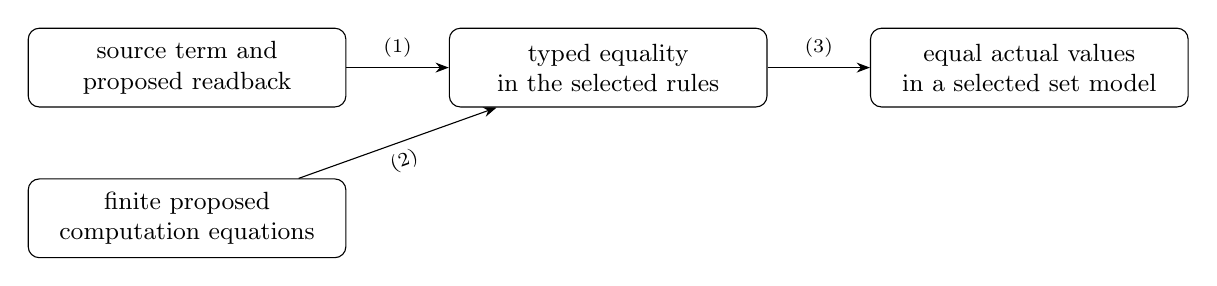
\begin{tikzpicture}[node distance=9mm and 13mm, every node/.style={font=\small},
  box/.style={draw,rounded corners,align=center,text width=38mm,minimum height=10mm},
  >=Stealth]
\node[box] (computation) {source term and\\proposed readback};
\node[box,right=of computation] (equality) {typed equality\\in the selected rules};
\node[box,right=of equality] (meaning) {equal actual values\\in a selected set model};
\node[box,below=of computation] (equations) {finite proposed\\computation equations};
\draw[->] (computation) -- node[above] {\scriptsize(1)} (equality);
\draw[->] (equations) -- node[below,sloped] {\scriptsize(2)} (equality);
\draw[->] (equality) -- node[above] {\scriptsize(3)} (meaning);
\end{tikzpicture}
\end{center}

Arrows (1) and (2) use the execution and equation-admission soundness theorems
above. Arrow (3), under a set model and annotation lifting, is realized by the
two \texttt{TowerInterpretation} companions:
\leanname{ExecutableEvaluation.run_existing_values} and
\leanname{EquationAdmission.existing_values}.  They compare independently
supplied typed annotations at every satisfying environment; neither supplies
universe assumptions or a model by fiat.  The native case compiler separately
checks a proposed recursor and every original equation before publishing its
fast computation clauses.  Native examples join ordinary execution, inspected
definitions, dependent proof functions, and GSLT proposals whose exact endpoints
are rechecked in the selected scope.  The natural-score selector has checked
size, sortedness, eligibility and conditional source-order stability properties.
These implementation qualifications do not establish a universal C refinement,
an arbitrary higher-order presentation exporter, or the completeness of the
selector's output from those four properties alone.

The three useful vertices are intensional mathematics, extensional mathematics,
and a language/operation presentation in GSLT-IL. These are semantic roles,
not three necessarily disjoint logics or three mandatory implementations.
HOL has inspectable proof syntax; a dependent calculus can have extensional
models. A single native dependent framework can expose a simple logical
fragment, a dependent fragment and a set-theoretic theory through different
interfaces, provided their interpretations and admitted extensions agree on
the promised overlap. In particular, a proposed \texttt{hol:} interface need
not imply a second proof kernel, and the \texttt{lang:} role need not be a
fourth mathematical foundation.

The categorical requirement is comparison respecting contexts and
substitution. In \nolinkurl{ComputationalTrinity}, contextual presentations
are presheaves and comparison maps are natural transformations forming a
commuting triangle. Invertibility is a stronger property: its explicit
information-loss control rules out a compatible inverse when a view forgets
a distinction. This abstract framework is not yet an instantiation of the
entire native DTT/HOTG/GSLT-IL triangle. The concrete family interpretation
below fills part of an edge, rather than assuming the whole triangle in a
record of required laws.

\paragraph{A simple fragment is a bridge, not automatic HOL adequacy.}
The formation-sensitive native embedding already preserves actual simple
terms and substitutions and characterizes conversion on its image.
Separately, the constant-family embedding is fully faithful in the selected
set-family contextual models. Neither result says that every native
inhabitant of a represented simple type comes from a source HOL proof.
The existing native HOL interface represents formulas and their substitution;
HOL equality is a declared proposition-former there, not native identity.
Realizing a HOL proof consequently requires a proposition/proof family and
the chosen logical rules, including the appropriate extensional principles.

There is a concrete interoperability hazard: HOL type variables range over
nonempty types, whereas a dependent host can express empty types. A translation
cannot silently extend that range to all host types. Assaf and Cauderlier
address this mismatch with inhabited-type representations in their combined
HOL/Coq development \cite{AssafCauderlierMixing}. Quantifier domains,
propositional truth versus proof inhabitation, universe levels, choice and
the added set axioms must likewise be stated at the selected interface.
These are focused mathematical obligations, not a demand to decide all
future language conventions.

\paragraph{What must precede an accelerated realization.}
Three levels of evidence have different dependencies:
\begin{enumerate}
  \item Mathematical coherence: actual interpretations of contexts, terms,
    proofs and substitutions, with the required equality and universe laws.
  \item Operational adequacy: the GSLT-IL presentation and its logical
    observations implement the specified mathematical tasks on the stated
    input domain.
  \item Realization and acceleration: the selected native implementation
    preserves those operations, and a comparison on the same task establishes
    any claimed performance benefit.
\end{enumerate}
The first level does not depend on generated NIK code. The second needs an
operational interpretation, but this may initially be a mathematical reference
semantics. Executable NIK qualification belongs to the third. The useful
reading of NIK as the language side hosting mathematics is therefore a
meaning-preserving realization of operations, not an independent source of
their truth. A fast implementation cannot establish the first two levels by
its speed or its regression tests.

OpenTheory is a plausible bootstrap route: Assaf and Burel translated its
standard library into a dependent logical framework while preserving binding,
typing and reduction \cite{AssafBurelHOL}. Their result is a precedent, not
an adequacy theorem for this native tower. Conservativity also has its own
theorems and hypotheses, as the functional-pure-type-system embeddings studied
by Assaf illustrate \cite{AssafConservativity}; it does not follow from merely
sharing arrow syntax. HOTG supplies another coexistence and theorem-transfer
precedent \cite{BrownKaliszykPakHOTG}, not permission to identify all the
extensional and intensional judgments globally.

\subsection{Biform theories and GSLTs as the semantic transformation waist}
\label{sec:biform-gslt}

Farmer's biform theory separates a formal language and axioms from executable
transformers, and attaches a meaning formula to each transformer
\cite{CaretteFarmerSharodaBiform,FarmerMohrenschildtTransformers}.  His
little-theories discipline additionally organizes mathematics as small theories
connected by inclusion and interpretation rather than one undifferentiated
foundation \cite{FarmerLittleTheories}.  The useful
correspondence here is not to introduce another intermediate representation.
A semantic stage is a GSLT, an implementation is a host machine equipped with a
faithful encoding, and a transformer is represented by retained operational
evidence.  Its \emph{meaning formula} is a sentence of the native mathematical
theory relating the denotations of its inputs and output; it must not be
identified with an operational simulation condition.  The formal biform seam
therefore pairs a closed theory in a $\pi$-institution with a proof-relevant
GSLT, assigns a native sentence to every retained primitive event, and requires
each such sentence to be a theorem of the closed theory.  A biform route carries
a logical theory morphism, a proof-relevant operational cover, and a naturality
equation saying that translation of the source meaning sentence is the meaning
of the translated event.  Hence event meanings transport compositionally while
remaining independently justified by the native consequence relation.

This contract has a nontrivial Henkin simple-type-theory discriminator.  A
Boolean machine retains one event, while its source meaning states equality of
two typed constants.  A non-injective signature map merges those constants; the
event and its meaning transport to the reflexive target equation, which is
valid in the target's empty theory.  If the source axiom is removed, the machine
still executes, but a separating Henkin model
proves that the same proposed meaning assignment is not sound.  Thus executable
behavior cannot certify its own mathematical interpretation.

A closed theory in a $\pi$-institution also induces a one-fibre NIK theory
family without selecting a checker: claims are native sentences, and scope and
meaning are the independently supplied closed theorem set.  Any proof calculus
with the exact theorem-image property supplies the corresponding native
evidence discipline, while a little-theory morphism supplies a heterogeneous
NIK semantic route.  The carrier of signatures in this one-fibre object is the
singleton selected signature, rather than the entire ambient signature
category.  This restriction is categorically necessary: identity and
composition of little-theory morphisms then map to identity and composition of
NIK routes on the whole object, not merely on its distinguished fibre.  The
construction is consequently a genuine functor from closed theories to
semantic NIK theory objects.  Naturality of proof projection proves that mapped
proof objects establish the translated sentence.

This bridge deliberately stops before Boolean replay: a checker and an exact
certificate boundary remain additional data.  For a biform theory, every
retained event has an inhabited native proof fibre for its meaning sentence.
Attaching primary NIK authority requires a claim-indexed equivalence between
the checker's accepted-certificate fibre and that native proof fibre; ordinary
scope authority is derived only after this stronger boundary is supplied.  A
paired discriminator equips the same valid Henkin equation first with the
canonical thin proof calculus and then with a Boolean-tagged calculus.  The
first fixed proof fibre is subsingleton; the second contains two provably
distinct witnesses with the same projected theorem.  No checker whose raw
certificate type is the singleton can be fibrewise equivalent to the latter.
Hence extensional theoremhood and certificate existence do not determine
intensional proof identity.

Proof authority therefore qualifies the biform graph rather than being
reconstructed from it.  A certified biform theory pairs a biform theory
with an exact executable certificate boundary for a selected native proof
calculus.  Its arrows carry a biform route and a certificate map, constrained
by a replay square that uses the sentence translation of that same biform
route.  These objects and arrows form a category with functors both to the
biform category and to the heterogeneous NIK authority category.  The image of
an arrow under the joint projection is exactly the replay-compatible locus.
A Boolean-tagged discriminator supplies two qualified endomorphisms with the
same biform identity: one retains the proof tag and one flips it.  Both replay
the same native conclusion, so the biform projection identifies them, while
the authority projection separates them.  Thus native certificate transport
is additional checked data even after operational meaning and theoremhood are
fixed.

The proof-relevant translations themselves form a category without first
quotienting their executable choices.  Equality of arrows includes the term
map, forward evidence map, and local evidence-lifting algorithm; identity and
composition preserve all three.  Biform theories consequently form a category
with separate functors to the little-theory category, the proof-relevant GSLT
category, and---by composing the first functor with the bridge above---the
semantic NIK category.  These projections have deliberately different
faithfulness.  In a checked discriminator, one endomorphism retains each of
two Boolean occurrence tags and another flips them.  Their native logical map
and every event meaning coincide, while the operational projection proves the
arrows distinct.  Thus strict categorical composition does not require
collapsing algorithm identity, and any later observational quotient must name
the consumer whose observations license that collapse.

Retained primitive events themselves form a covariant functor from the
proof-relevant GSLT category to types.  The corresponding biform event functor
is its composite with the operational projection.  Consequently the
observer-relative constructions below depend only on this event action and on
their declared value map; they do not depend on the logical projection except
when a biform meaning theorem is also requested.

The joint logical--operational projection is sharper than either forgetful
view.  On every hom-set, its image is exactly the locus of pairs consisting of
a little-theory map and a proof-relevant operational map for which the event
meaning square commutes.  The pair determines the biform route uniquely, but
an arbitrary pair need not be a route: a checked tag-sensitive example has
well-typed logical and operational components whose meaning square fails.
Conversely, a second Henkin discriminator keeps the operational map fixed while
changing the translation of typed constants, so the operational projection is
not faithful either.  Thus the biform category is not a product of independent
IR components; it is the compatibility locus inside that product.  This gives
the categorical statement of why a useful intermediate language retains both
an executable transformation and its mathematical meaning without identifying
them.

Observer-relative control factors through the proof-relevant event action at
an even weaker layer.  A map of events pulls target occurrence indices,
observers, client contracts, and scheduler readouts back to source histories,
while concrete changes and their complete removal ledgers map forward.  These
actions respect route composition.  If the target occurrence index is exact,
its pullback is exact precisely when the event map is injective.  A checked
Henkin biform route exhibits the boundary: it preserves the native theorem
assigned to every event and preserves a length observer and an accounted
reordering, while merging two Boolean occurrence witnesses into one target
event.  Exact occurrence identity therefore fails to pull back.  Mathematical
meaning, client observation, and proof-occurrence identity are three distinct
contracts, even when they travel along the same route.

Separately, an exact transformer between semantic stages may carry the
following two operational directions:
\[
  s\longrightarrow_S s' \;\Longrightarrow\;
    f(s)\longrightarrow_T f(s'),
  \qquad
  f(s)\longrightarrow_T t \;\Longrightarrow\;
    \exists s'.\;s\longrightarrow_S s'\land f(s')=_E t.
\]
The second clause is intentionally modulo the target equations.  Together the
clauses define an equation-class cover; such covers compose and induce exact
transport of the generated modal observations.  When proof occurrences are
public, a stronger arrow carries an equivalence of the complete evidence fibre
at each pair of endpoints.  More general compiler transformations may instead
map one source step to a finite target path; fusion, lowering, and exact covered
translation are deliberately different grades rather than one overloaded
notion of morphism.

An equation-class cover is not yet a literal covered map of representatives.
Quotient completion sends every represented GSLT to its term classes and every
equation-class cover to a covered translation whose lifted endpoint is now
literally equal.  Consequently any functor from a pass index into represented
languages induces the existing covered GSLT diagram after quotient completion.
Formula transport requires the additional observation and label maps, with
their satisfaction and action naturality laws; it does not follow from a bare
term translation.

This gives parser compilation the same shape as symbolic mathematics.  The
scannerless source judgment is one proof-relevant GSLT, the compiled ParserPack
judgment is another, and compiler correctness is an exact GSLT arrow between
them.  Tables, charts, forests, and host-language plans implement the target
step relation but are not semantic pipeline nodes.  OSLF and the native type
theory are generated from the two GSLT endpoints.  Successful compilation is
sealed as one package containing only the target proof-relevant GSLT and the
exact arrow from the source; the concrete plan is hidden behind that package.
A real RFC~8259 instance
preserves and reflects the entire root-derivation fibre, including production
occurrences, spans, zero-width steps, and administrative end-of-input evidence;
a malformed target profile cannot acquire an exact arrow.

The same criterion disciplines a Felix- or ForTheL-like mathematical surface
\cite{KoepkeDeLonLorenzenForTheL}: parsing, notion elaboration, logical
elaboration, optimization, and runtime realization are composable GSLT arrows.
Their host data structures remain private realizations.  A weak notion normally
lands in the simple higher-order predicate fragment; an evidence-indexed notion
lands in the dependent fragment.  Quotation and evaluation are admitted only
through a declared syntax boundary and a meaning theorem, rather than by
silently identifying syntax with denotation.  The explicit parse-tree data
advocated by that work is retained as a term and evidence object of the parsing
GSLT; it does not become an unverified semantic intermediate language.

\subsection{A theory graph rather than one maximal kernel}

The preceding operational waist is only one face of the desired system.  A
GSLT records terms, an equational congruence, and dynamics; it does not by
itself provide the models, satisfaction relation, dependent judgments, or
foundational strength of every logic that may use those dynamics.  Conversely,
a mathematical theory with no useful operational rules need not be forced into
a vacuous GSLT merely to enter the library.

Institution theory supplies the outer, logic-independent interface
\cite{GoguenBurstallInstitutions}.  It separates a category of signatures,
sentence translation, contravariant model translation, and satisfaction, with
the satisfaction condition requiring truth to be invariant under change of
notation.  The little-theories graph can therefore contain classical simple
type theories, dependent type theories, set theories, modal logics, and proof
systems without identifying their native judgments.  The formal development
now contains this model-valued structure directly.  Every institution induces
its semantic-consequence $\pi$-institution, and every model-valued comorphism
projects to a consequence-preserving comorphism; the earlier consequence graph
is therefore a forgetful view rather than a competing formalism.  This
projection is a functor between the corresponding heterogeneous categories:
it preserves identity and composition, but is not faithful because distinct
native model actions can induce the same consequence route.  Predicate
models generated from an arbitrary semantic carrier functor give a reusable
test family: sentence translation follows the carrier naturally, models reduce
by inverse image, and the satisfaction square commutes.  A direct-image
falsifier on Booleans proves that the contravariant model direction is semantic
content rather than bookkeeping.

The model-valued institutions are also bundled with their native signature
categories into one heterogeneous category whose arrows are institution
comorphisms.  This supplies composition across genuinely different logical
languages without first translating them into a common syntax.  The
constant-family simple-to-dependent comorphism is an actual arrow of this
category and is provably noninvertible: a two-sided inverse would put the
varying Boolean family in the essential image of the constant-family functor.
Thus the theory graph supports fluid movement between simple and dependent bubbles
while retaining a checked reason that the latter cannot be globally collapsed
to the former.

Conservative transport admits an isomorphism-safe refinement.  Literal model
coverage is sufficient for reflection of semantic consequence, but is stronger
than the mathematical requirement when model presentations differ.  Coverage
up to model isomorphism composes and also reflects consequence provided the
source satisfaction relation is invariant under model isomorphism.  The latter
condition is not derivable from the bare institution laws, which govern change
of signature rather than change of model representative.  A checked negative
institution contains two isomorphic model objects that disagree on its unique
sentence: a comorphism covers both up to isomorphism, but consequence reflection
fails.  Ordinary predicate institutions satisfy the invariance premise.  Hence
theory-graph routes may use representation-independent coverage without silently
assuming that every native notion of observation is extensional in model
identity.

The first concrete logical node is now present for a precisely qualified
Church-style simple type theory: the alphabet of base types is fixed, typed
constant signatures and closed formulas vary functorially, and extensional
Henkin models reduce contravariantly.  The satisfaction condition is proved by
commutation of term denotation with constant translation.  The model class
includes the function-extensionality property required by the extensional
derivation calculus, so finite derivability is proved to imply institutional
semantic consequence.  A non-injective signature map that merges two constants
preserves the satisfaction square but provably fails to reflect validity; this
separates an arbitrary institution morphism from a conservative embedding.

The corresponding property-explicit theory-graph node adds excluded middle,
schematic Hilbert choice, and Dedekind infinity at one selected base type.  It
enters as a logical-only node: no transition system is fabricated for it.  A
later machine may provide an operational face only by mapping each equation
class of states to a qualified Henkin model.  This construction is not yet a
full category of HOL signatures varying base-type operators, and it does not
make choice, infinity, or extensionality implicit in every simple type theory.
Concrete institutions for the selected dependent and set-theoretic proof
systems remain obligations; the generic institution interface itself does not
supply their soundness or completeness.

An inter-bubble route can consequently carry two independent contracts:

\begin{enumerate}
\item an operational GSLT translation, graded as forward, covered, or
  proof-fibre exact; and
\item an institutional translation or comorphism preserving the declared
  consequence and satisfaction judgments.
\end{enumerate}

Only a commuting pair earns a claim about both execution and mathematical
meaning.  This is the appropriate place for linking-type annotations: a
component reasons in its own language, while the boundary explicitly records
which foreign behavior is admitted and which equivalence theorem survives
linking \cite{PattersonAhmedLinkingTypes}.  NIK supplies admission and replay
authority for such routes; it is not a substitute for either semantic law.
The formal theory graph realizes this separation by giving every node a native closed
theory and only an optional operational face.  Nodes with an operational face
and commuting routes form a category with separate forgetful functors to the
logical theory category and the equation-class-covered GSLT category.  Thus a
pure mathematical theory needs no dummy transition system, while a compiler
route cannot acquire a mathematical meaning theorem merely from step
preservation.  Composing the logical projection with the closed-theory NIK
functor gives the semantic authority view of every equipped node.  This view is
intentionally lossy: a checked hidden-state refinement has the same NIK object
as its visible source, yet contains a concrete private operational state
outside the source representation's image.  Therefore the operational,
logical, and authority projections coexist in one commuting architecture
without any one of them being advertised as recoverable from another.

The model and operational readings now meet constructionally.  A
model-qualified operational face maps each equation class of machine states to
a model of its native signature.  The interpretation of a sentence is simply
satisfaction in that state-indexed model, so equation invariance and semantic
consequence soundness are derived rather than separately postulated.  Forgetting
the models only after this construction recovers the consequence-level
operational face.

There is also a first nontrivial simple-to-dependent institution route.  Over a
fixed context, the simple side uses one value type at every context point and
the dependent side admits an indexed family; total-space predicates supply the
models on both sides.  Constant-family inclusion induces an institution
comorphism whose satisfaction square is exact.  Over the two-point context its
signature functor is faithful but not full, and the family with a singleton
false fibre and a Boolean true fibre is provably outside its essential image.
The route also covers models: every simple predicate model is literally the
reduct of the same predicate on its constant-family carrier.  A generic theorem
therefore proves preservation and reflection of semantic consequence on the
translated sentence image.  This hypothesis has content beyond satisfaction
preservation: a checked comorphism collapsing two Boolean sentences to one
still satisfies the institution square but cannot lift the source model
$\{\mathsf{false}\}$, so it does not reflect consequence by this criterion.
This is the precise scoped answer to whether dependent types are justified:
not for objects already in the constant-family image, but necessarily for a
consumer that must preserve genuinely varying fibres.  It remains a semantic
specimen, not yet a complete institution for either a concrete Church-style
simple type theory or a selected dependent proof calculus.

The selected-theory layer now varies the consequence institution as well as
the signature.  Its objects are closed theories in their native
$\pi$-institutions.  An arrow consists of an institution comorphism, a map from
the translated source signature into the selected target signature, and a
proof that every selected source theorem lands in the target theory.  These
arrows compose, and the ordinary category of closed theories over any fixed
institution embeds faithfully as a vertical fibre.  Thus the heterogeneous
theory graph replaces neither the existing little-theory categories nor their native
sentences; it organizes them in one total category.

The biform layer has the corresponding heterogeneous total category.  Its
arrows pair a cross-institution closed-theory map with a proof-relevant GSLT
translation, subject exactly to the commuting event-meaning square.  The image
of the projection to the independent logical and operational arrows is proved
to be the compatible locus, and every fixed-institution biform category embeds
faithfully as a vertical fibre.  The simple-to-dependent comorphism supplies a
nontrivial positive specimen: two distinct retained operational occurrences
cross the logical boundary while their translated meaning theorem is
preserved.  A negative specimen changes the target meaning sentence while
retaining the same logical and operational arrows; the compatibility square
fails and no biform arrow exists.  This is the checked categorical form of a
multi-level intermediate representation: native logics remain native, GSLT
events remain proof-relevant, and only their justified commuting pairs can be
composed as meaning-preserving transformations.

Executable proof authority now lifts over this heterogeneous biform category as
well.  Each object selects its own native proof calculus and an exact certificate
boundary; each arrow adds a certificate map whose Boolean replay commutes through
the very same cross-institution sentence translation used by the biform arrow.
The fixed-institution authority categories embed faithfully as vertical fibres,
and the joint image is exactly the replay-compatible locus.  In the
simple-to-dependent specimen, native thin proof objects cross the logical
boundary exactly.  Keeping the same biform arrow while sending its source
certificate to a different target theorem is a checked negative: theorem
preservation and event-meaning compatibility do not manufacture replay
authority.

This also sharpens the role of GSLT-IL.  It is an operational language for
sitting at a represented stage and moving along typed routes between stages,
not a universal proof foundation and not a lowest-common-denominator term
format.  A reflective surface language may orchestrate that graph, but no
surface becomes the ``ultimate IR'' merely by being able to quote all the
others.  Stronger bubbles stay available without imposing their conversion,
identity, or universe rules on weaker consumers.

The categorical accounts of operational semantics explain why this separation
is productive rather than bureaucratic.  Turi and Plotkin combine an algebra of
syntax with a coalgebra of behavior through a distributive law, obtaining a
compositional operational model and a canonical denotational model under
explicit hypotheses \cite{TuriPlotkinMOS}.  Recent categorical semantics for
SSA likewise gives an IR its own equational theory and proves soundness and
completeness against categorical axioms \cite{GhalayiniKrishnaswamiSSA}.
MLIR supplies the engineering analogue: several dialects retain the invariants
needed by their own transformations and lower progressively rather than
reconstructing high-level facts from one premature low-level form
\cite{MLIRRationale}.  An equality-saturation dialect sharpens the same
lesson: retaining the e-graph in the intermediate representation lets ordinary
passes coexist with nondestructive equational rewriting instead of extracting
one representative after each phase \cite{EqSatDialect}.  In the present
setting this is one possible operational GSLT dialect, not a global identity
principle: its equations, extraction observer, and cost model remain explicit.
The semantic content of the multi-level practice is a diagram of GSLTs and
independently justified models, with the strength of each arrow stated rather
than inferred from the word ``compilation''.

Collapsing the internal execution of one representation into a coarser step
does not erase that representation's equality.  Given a run protocol, a raw
run is a finite path from the protocol's entry state to a designated exit
state, while its semantic run view is
\[
  E\mathbin{;}\mathsf{Run}\mathbin{;}E.
\]
This view inherits the represented language's generated setoid, and a cover by
runs lifts target executions only up to that same setoid.  Syntactic equality
is recovered by theorem when the presentation generates no equations; it is
not a parallel equation-free interface.  A four-constant discriminator makes
both endpoint changes essential: with $A=_{E}B$, $C=_{E}D$, and a protocol
recognizing only $B\mapsto C$, the raw relation does not connect $A$ to $D$
but the semantic run view does.  Thus a compiler or parser pipeline may use
language definitions and GSLT morphisms at every semantic node while retaining
private host data merely as an implementation of an arrow.  No result here
depends on rho-calculus minimal contexts: those are needed only for the
rho-specific contextual labels in its modal adequacy theorem
\cite{MeredithFindingMind}.

\subsection{Observer refinement, dependent descent, and several identities}

There is no single useful chain called equality.  At least the following
relations have different elimination principles and different consumers:

\begin{enumerate}
\item judgmental conversion, used silently by a checker;
\item the authored and derived GSLT congruence $E$, used to choose semantic
  operational states;
\item intensional identity or path evidence, used by dependent elimination;
\item behavioral equivalence relative to a chosen family of observations and
  labeled interactions;
\item extensional equality in a selected mathematical model; and
\item diachronic lineage, represented by retained routes between temporally
  distinct states rather than by endpoint equality.
\end{enumerate}

These relations may coincide in a scoped profile, but the coincidence is a
theorem, not conversion.  In particular, quotienting by the symmetric closure
of operational steps computes connected components.  A two-state system with
one transition has equal component classes although its source and target are
not bisimilar.  This checked counterexample prevents the
operational--intensional--extensional diagram from silently reclassifying
reachability as identity.

Observer refinement gives the precise refinement law.  Suppose every coarse atom and
label has an exact representative for a finer observer, while the fine observer
may ask additional questions.  Every coarse modal formula then has the same
truth value after translation, and fine behavioral identity implies coarse
behavioral identity.  Hence there is a canonical contravariant map
\[
  \mathsf{Class}_{\mathrm{fine}}
    \longrightarrow \mathsf{Class}_{\mathrm{coarse}}.
\]
If the atom and label maps are also surjective, this map is injective and the
two observers induce the same identity.  Without that hypothesis it can merge
classes: a checked inert Boolean system is indistinguishable to an observer
with only the always-true question and distinguishable to one that may inspect
the Boolean state.

The dependent consequence is exact.  All equality families anchored at fine
behavioral classes descend through the coarse class map if and only if that map
is injective.  Individual families can still descend through a lossy refinement when
they are constant, up to the selected equivalence, on every merged fibre.  This
is the formal version of fluid abstraction: ordinary reasoning inside a coarse
bubble remains legitimate, while refining back into a distinction that was
forgotten requires retained evidence or a reconstruction theorem.

It also gives a non-rhetorical answer to whether dependent type theory is
justified.  Simple type theory is the preferred mathematical interchange when
types and conclusions are constant on the relevant fibres.  Dependency is
earned when an earlier response, proof, revision, observation, or route selects
the type of later data.  For example, $n-1+1=n$ is false for natural numbers at
$n=0$; the missing lower-bound evidence is real information, not a defect of
dependent syntax.  One may instead work in integers, retain the guard as a
dependent premise, or cross a boundary that states exactly what is forgotten.

Observational type theory and two-level type theory are therefore valuable
candidate bubbles rather than mandates for the common core.  The former keeps
decidable definitional equality while supporting an explicit substitutive
extensional equality \cite{AltenkirchMcBrideOTT}; the latter separates strict
and weak equality without requiring global equality reflection
\cite{AltenkirchCapriottiKraus2LTT}.  The shared contract remains dependent
identity elimination with its computation and substitution laws.  Primitive
$J$, cubical transport, observational equality, and scoped UIP are alternative
realizations whose use must be selected and qualified locally.

Hofmann's translation programme explains why this should be a bridge rather
than a global switch: extensional equality reflection makes typing
undecidable, while partial-equivalence-relation and family models recover
extensional quotients inside an intensional host; the simple PER model does not
support genuinely varying dependent families, and the richer family model pays
for that power with more complicated coherence and some conversion laws only
up to propositional equality \cite{HofmannExtensionalConcepts}.  Accordingly,
an extensional bubble is a certified quotient/model readout of an intensional
one when such a model theorem is available.  It is not permission to add
equality reflection to every checker.

\paragraph{Mutable references admit different comparison contracts.}
For allocated references $a,b$ in a heap $H$, three coherent scalar
comparisons are location identity $a=b$, current-payload equality
$\mathsf{read}_H(a)=\mathsf{read}_H(b)$, and equality of the payloads in a
fixed captured heap $H_0$. The existing
\leanname{ResourceOwnership.MutableObservation} construction realizes all
three on one nonempty heap. Current-payload equality is an equivalence at
each fixed heap. Capturing the heap yields a pure frozen comparator;
changing its heap argument yields a world-indexed comparator. A fixed
world-independent comparator cannot also track equality in every pair of
independently writable current worlds. This rules out that combination of
promises, rather than ruling out observation-based comparison.

The available program experiments determine stronger requirements. The
existing \leanname{PolicyFamily.ContextClosure} construction closes a
specified observation family under finite paths of declared total state
operations. It constructs the greatest observation-preserving relation
stable under those operations. The
\leanname{ResourceOwnership.Optimality.ContextualReferences} instance uses
actual heap payload writes at the selected reference, followed by a scalar
read at that reference or a fixed anchor. With allocated references, two
distinguishable payload values, all such writes and all fixed-anchor reads,
its contextual equivalence within a fixed initial heap is exactly location
identity. A one-write path already separates distinct cells: writing at the
hole and reading a retained alias sees the write only when the locations
alias. Two different write values remove any assumption about the old
payload. Every readout realizing this entire experiment family must
therefore preserve the selected-reference distinction within that heap.
An address alone is not thereby a sufficient readout across different heaps.

A second writable profile restricts this same operation graph to observations
of the selected cell alone. The
\leanname{ContextualReferences.SelectedOnly} construction reuses the existing
consumer restriction and greatest stable relation. Its concrete update law is
\[
  \mathsf{selectedRead}(\mathsf{write}(v,c))
   =\mathsf{map}(\lambda\_.v,\mathsf{selectedRead}(c)).
\]
Consequently equality of selected scalar observations is preserved by every
write and characterizes the resulting finite-context equivalence, even
across different heaps. The two allocated cells with payload $7$ remain
equivalent under this interface after genuine writes to $9$; the fixed-anchor
interface still separates them. Mutation alone therefore does not force
location identity. The available observations and operations determine which
replacement law is justified. The total model separately distinguishes honest
absence from an allocated value; it does not model denied service as absence.

Nested resources refine the same method without selecting a graph equality.
An ordinal path is an actual adaptive query over the admitted ordered
descriptor rows: every visited header is recorded, repeated slots remain
repeated, and a missing endpoint is an ordinary negative reply. For fixed
finite read paths and write paths, the observable signature consists of the
initial scalar-read vector and the matrix stating whether each write path and
read path reach the same allocated endpoint. The concrete payload-update law
proves this signature stable under all declared writes. Conversely, when the
payload has two distinguishable values, two write probes recover every matrix
entry. Thus the existing finite context closure equates two clients exactly
when their signatures agree.

A shared diamond and a duplicated diamond can therefore agree under read-only
or selected-descendant observations, while writing through one arm and reading
the other separates them. Finite paths also observe self and mutual cycles
without unfolding an infinite tree. Reordered and repeated slots show why the
reference set alone is insufficient for an ordinal query. A conservative
candidate preview keeps an unknown read, distinguishes it from known absence,
and filters original occurrence coordinates and bindings rather than replacing
them by candidate-list positions. This is a theorem about the declared finite
resource profile; native State/Space matching and arbitrary graph
isomorphism or bisimulation remain separate instances.

The same two equal-valued cells satisfy the read-only family and fail the
write-closed family. Restricted read grants and a one-value payload type
give further separating controls against unconditional identity necessity.
Equal scalar observations imply neither shared authority nor equal
generation or origin. Relocation transports actual writes, reads and aliases
through the existing injective address map; a fresh isolated clone retains
its internal sharing without becoming the original mutable resource.
These are scalar-payload results, not recursive graph equality or a model
of every source-language context. The total-write profile treats absent
addresses as absent, not as service refusal. Constraint-based unification,
linear or persistent state, graph isomorphism and bisimulation require their
own constructions and comparison laws.

Collection and typing contracts must state which of these observations they
consume. Stable resource keys, frozen value keys and validated
world-dependent value indexes have different preservation obligations;
value-based queries do not automatically require a linear scan. Scalar
read observations remain valid after a write outside their actual resource
support. Freezing such a readout does not freeze every resource reachable
through its payload. Likewise, a Boolean comparison does not automatically
provide intensional identity evidence, judgmental conversion or a license
to replace references through arbitrary effects. These constructions
delimit compatible promises without selecting a global meaning for the
surface equality operator.
An observational equivalence theorem also does not supply a terminating
Boolean test for arbitrary payload types. Executable scalar comparison uses
the stated decidable-equality premise; richer observations still need their
own decision or retained partial-computation contract.

\subsection{Compositional execution contracts over worlds and runs}
\label{sec:execution-contracts}

An execution contract selects a program semantics, the resources and services
it may use, its observable outcomes and commitments, and the applicable
progress and cost comparisons. These are obligations over a common execution
object, not interchangeable meanings of one numerical weight. Epistemic
authority qualifies a judgment and its evidence; resource authority describes
held rights. A service assumption can justify conditional reasoning about a
run without becoming checked evidence or an execution grant.

\paragraph{Resource authority and reification.}
Let $A$ be a separation algebra, with compatibility $p\mathbin{\#}r$ and
composition $p+r$ defined lawfully on compatible resources. A reification
$V:A\to\mathcal P(S)$ interprets authority as sets of machine states.
For an action relation $a:S\to S\to\mathsf{Prop}$, the frame judgment is
\[
  \mathsf{AP}(V,a,p,q)
  \quad\Longleftrightarrow\quad
  \forall r,\ p\mathbin{\#}r\Rightarrow
  \forall s\in V(p+r),\ \forall s',\
  a(s,s')\Rightarrow
  q\mathbin{\#}r\ \land\ s'\in V(q+r).
\]
This is the existing \leanname{Contracts.ActionPreserves}, following the
Views interpretation of concurrent reasoning
\cite{DinsdaleYoungViews}. Rely--guarantee claims instantiate the same
separation algebra: assertions are stable under their rely, and compatibility
requires each guarantee to lie within the other's rely
\cite{JonesInterferingPrograms}. These laws prove safety of completed
interleavings. They do not equate their visible traces or establish that a
particular waiting task receives service. Enabledness is separate: an action
that never runs from the admitted view can satisfy this safety judgment
vacuously.

\paragraph{Relational transport with a frame back law.}
Suppose $f:A\to B$ is a resource homomorphism and
$R:S\to T\to\mathsf{Type}$ is a proof-relevant relation. The reification square
is
\[
  t\in V_T(f(p))
  \quad\Longleftrightarrow\quad
  \exists s\in V_S(p),\ \mathsf{Nonempty}(R(s,t)).
\]
Target steps must reflect along the selected relation witness: from
$R(s,t)$ and $b(t,t')$, obtain an $s'$ with $a(s,s')$ and $R(s',t')$.
The resource back law lifts every compatible target frame:
\[
  f(p)\mathbin{\#}u
  \quad\Longrightarrow\quad
  \exists r,\ p\mathbin{\#}r\ \land\ f(r)=u.
\]
\begin{proposition}[Transport and composition of the frame judgment]
Under these three conditions, $\mathsf{AP}(V_S,a,p,q)$ implies
$\mathsf{AP}(V_T,b,f(p),f(q))$. Two such adapters compose by resource
homomorphism composition and by the existing horizontal relation
\[
  (R;Q)(s,u)=\sum_{t:T}R(s,t)\times Q(t,u).
\]
\end{proposition}
\begin{proof}
Lift an arbitrary target frame to a source frame, recover a related source
state through the reification square, reflect the target step, and apply the
source frame judgment. Reify its successor and map its compatible frame
back to the target. For composition, retain the actual middle state and both
relation witnesses; frame lifting and step reflection compose through that
same middle representation. The checked endpoints in the
\leanname{ActionPreserves} namespace of
\leanname{GSLT.Contracts.ReifiedActions} are
\leanname{transport_relation},
\leanname{ReifiesThrough.comp},
\leanname{ReflectsThrough.comp}, and
\leanname{transport_relation_comp}.
\end{proof}

The controls are substantive. Exchanging two owned cell locations transports
the write judgment. Adding an effect log gives a relational representation
whose frame-safe actions can emit $[\mathsf{false},\mathsf{true}]$ or
$[\mathsf{true},\mathsf{false}]$ while leaving identical owned cells.
Conversely, forgetting one cell's authority admits a reification square and
step reflection for a target action that overwrites both cells; it breaks
the forgotten cell's independently held frame. Thus the first two conditions
alone do not justify the general transport rule, and a frame-safe adapter
still owes its selected observation comparison.

World-indexed resource transport has the covariant opfibration constructed
in \leanname{Contracts.IndexedAuthority}. Its base arrows are already
selected changes of world; the cocartesian lift does not authorize an actor
to take an arbitrary arrow. Cartesian lifts require the stated right-adjoint
law. The constructed all-access revocation example fails that law; this is
not a claim that every information-losing transport lacks a right adjoint.
Contravariant predicate reindexing remains a different, compatible role.

The retained occurrence-space instance in
\leanname{Contracts.OccurrenceSpace} reifies complete ordered key/version
rows using fractional read shares and whole update shares. Actual local
replacement and the existing keyed consuming publisher satisfy the frame
judgment for every compatible other-space frame. Bijective namespace
transport constructs the reification, extension-lifting and action laws;
identifying namespaces can destroy them. This is a nonempty store instance,
not an additional evaluator. The publisher's real admission establishes
unique stable keys. Frame safety alone neither establishes this uniqueness
nor licenses reordering the resulting publication history.

\paragraph{Actual adaptive reads determine transaction dependencies.}
For a finite ordered occurrence store $s$, let
$\mathsf{rows}(q,s)$ be its full list of matching identifier/payload pairs.
The certificate of a read records both the complete ordered identifier list
and the presence of each corresponding payload. Under the explicit integrity
condition that one identifier has one payload in the current store,
validation of this certificate is equivalent to equality of the full row list.
The equality retains multiplicity, including distinct occurrences with equal
printed values.

\leanname{Contracts.Dependencies.valid_readDependencies_iff} connects those
concrete certificates to the existing \leanname{Machines.ReadOnlyQuery}
interpreter's actual read agreement.
\leanname{validated_adaptive_query} consequently preserves its entire
observation, including the answer-selected query path.
\leanname{readDependencies_bind} appends the actual continuation's
dependencies; \leanname{validated_adaptive_resume} validates the performed
prefix before querying a fresh suffix. A coexisting environment run
establishes that same validation premise. Unrelated insertions preserve the
constructed adaptive query; inserted child matches, changed payloads and
ambiguous identifiers distinguish invalid certificates. An empty child
answer still contributes a complete-query dependency.

These are laws for the pure occurrence-query profile with fixed program and
query meanings. The constructed \leanname{ReadOnlyQuery.ScopedOccurrence}
provider additionally transports complete cross-space replies, retained
continuations and exact read accounts through a namespace equivalence.
Metadata validation preserves full adaptive replies only under the explicit
immutable $(\mathsf{epoch},\mathsf{full\ stamp})$-to-payload interpretation;
an unversioned mutable-payload control violates the conclusion. The existing
own-write client retains captured reads across its actual local update, and
the channel publisher supplies the general consuming case.
\leanname{ChannelJoin.AuthorizedPublication.adaptive_publication_preserves_frame}
joins current delegated grants, full adaptive row observations, selected
observers and the actual keyed take/output operation at one boundary.
The \leanname{ReadOnlyQuery.RetainedForce} adapter separately checks the
current located Need lease and complete generational binding reference:
copied descriptions do not grant force authority. Native higher-order
matching, arbitrary imported-code/captured-world transport, service authenticity,
fairness and physical costs retain their own realization obligations.
Snapshot continuation and validated-fresh resumption remain distinct.

\paragraph{Committed observers and nondiscardable obligations.}
For a dependent observer family $O(s):\prod_{i:I}D_i$, administrative
preservation holds exactly when it holds componentwise. Erasure likewise
preserves a committed family $O$ against retained family $H$ exactly when
each $O_i$ agrees with $H_i$ at every erased administrative dead end.
The checked endpoints are
\leanname{OrderedSystem.administrationPreserves_family_iff} and
\leanname{OrderedSystem.erasurePreserves_family_iff}. The family may therefore
include separate permission, duty, disclosure or history readouts without
coercing their carriers into one algebra.

Frame-preserving updates permit relinquishing authority. They do not thereby
settle an obligation already incurred. The constructed
\leanname{Contracts.Joins.duty_family_requires_retention} control permits
erasure at an empty permission observer and refuses it at an outstanding-duty
observer unless the duty is retained outside the rejected leaf.
The existing attempt-identity owner now supplies concrete allocating,
transferring, supervising and settling transitions. Its
\nolinkurl{DurableDuty.issued_duty_conservation} theorem derives, from an
arbitrary finite run starting at the empty ledger, exactly one retained row
for each issued occurrence. The row has an authorized ownership chain and
either remains unsettled or records an authorized disposition. The original
obligor, obligee and scope survive transfer; copying a descriptor does not
allocate another occurrence. Atomic publication validates the current
authority data together with the ledger, so a changed grant cannot hide
behind a reused revision. Authentication of that authority data remains a
service assumption.

The existing dispatch-permit owner instantiates this ledger with an escrow
service using its one-use dispatch claim and the existing supervisor. For
every fresh funded reversible reservation, its actual debit followed by
refund restores the original balance while retaining the ordered debit and
refund events. Replaying the refund is inert; treaty satisfaction is derived
from the actual refund history rather than assumed from a compensator's
name. Intention, dispatch, remote acceptance, completion persistence and
adoption are distinct transitions. Primary and repair crash controls retain
uncertainty until positive reconciliation; missing acknowledgment does not
prove failure. Irreversible effects refuse compensation. The construction
does not prove eventual settlement or compiled-C refinement.

The dispatch-permit owner's retained-settlement construction joins the actual
escrow adopter to the existing indexed query, paid invocation and publication
interfaces. Its adaptive query reads service state, current application grants
and independent receiver evidence. A successful readout is computed by the
adopter, with an explicit refusal for absent or inconsistent evidence. Reachable
execution derives readiness from that query; it does not assume agreement of
complete runs. Pausing, refusing, rearming and changing the handler preserve the
recorded reads, residual query and paid account. Accepted publication revalidates
those dependencies and the exact host-grant generation. The resulting current
adoption preserves the duty ledger and has actual receiver evidence, without
performing another remote effect. A second chronological read-provider
representation supplies a handler homomorphism preserving the local reply,
gates, replay policy and ordered invoice. These are model theorems; authentic
native decoding, handler correspondence and physical operation prices remain
separate obligations.

The maintained native activity library realizes concrete HE and retained Prime
clients of this boundary. A state context wraps the existing activity continuation without
changing its proposed writes or sends. The enclosing duty retains its original
parties, current custody, primary and repair activities, disposition and
history. Current policy records authorize issue, transfer, execution and
disposition separately. A correlated completion survives cancellation or
execution revocation; settling it additionally requires the current holder's
adopt/compensate right and a trusted interpretation of separately captured
receiver evidence. The atomic host commit revalidates the exact policy,
result and evidence records, including a same-byte replacement at a new
revision. A contract tag or worker assertion alone is insufficient.
The independent receiver fixture actually debits and refunds native stored
funds while retaining both historical effects; it also exercises primary
adoption, restart after debit and irreversible refusal. These are native
boundary controls with explicit principal-binding and receiver-authenticity
assumptions. Retained Prime imports the same client through the compiled source
reader and document-scope elaboration. Its captured context retains structural
mechanism availability and the explicitly admitted owned Rho handlers, but no
loader or unrestricted external-service authority. Equation lookup uses frozen
code, while the context-space operation and module-bound self reference
designate the private data world. A computed storage coordinate is evaluated by
the retained operand continuation. Policy revocation and equal-right regrant
before commit refuse the stale issuance.

The Prime reply path uses the existing owned-return sequencer for canonical
Rho reduction and ordered value observation. The reducer retains its canonical
cursor and the Prime payload provider; synchronous and resumable value
observation use one traversal. A refused delivery retains the exact completed
occurrence, and retry does not rerun the reducer. Callable-looking payload data
and duplicate occurrences remain data and duplicates. The generic evaluator
frame holds only an optional service pointer. The service retains its cursor
owner and prevents moving collection or promotion while that opaque state is
live. Each advance and delivery rechecks its selected context and caller
contract; payload execution inherits the caller's permit chain. The generated
progress declaration admits the owned handler and excludes its atomic prepared
shortcut. Native controls cover all three HE/Prime duty scenarios, incomplete
service failures, stale result arenas, allocation refusal, cancellation and
split observation. These logical cursor transitions do not bound the internal
work of preparation, normalization, allocation, materialization or teardown.
This selected native control supplies neither arbitrary imported-world
refinement nor a physical responsive-slot theorem.

Deferred native payloads now preserve the captured code/data distinction through
nested space overlays. The copied registry retains an explicit self binding;
the context operation recognizes transparent views of its selected program,
without treating a module-own view or unrelated space as that context. The
shared space resolver consults each frame's direct raw-reference override before
its inherited visible alias, so entering an empty frame preserves the preceding
observation. A visibility redirect alone cannot license mutation: child writes
use storage owned by that child, while borrowed parent views remain unchanged.
Raw and already-visible references share the same newly created Rho overlay.
Native controls exercise omitted and non-space self bindings, nested own writes,
raw overrides, identity redirects and module-own boundaries. These are tested
native service laws, not a compiled-code refinement or an ownership acquisition
for arbitrary external services.

The transaction frame is now address-stable and independently owned. A suspended
child retains its original parent frame, including scratch resources; activation
holds both the selected frame and the displaced caller until restoration.
Synchronous and retained payload calls share overlay preparation and result
promotion. An optional native provider retains the ordinary Prime stack, its
Need episode and return traversal. Initialization runs the existing top-level
prelude; only its designated heap result receiver can retain the final expression
call. Thus registry-returned stored descriptors remain data, held values keep
their top-level fuel exception, and incomplete preparation cannot become an empty
completed frontier. Each grant borrows the current caller's authority rather
than retaining a previous driver. Scoped library selection preserves session
options. A failed provider prefix supplies no COMM candidate, and retirement
does not require permission to advance. Referenced source services and result
resource owners remain caller-held. Prelude, preparation, native operations,
copying, promotion and teardown still require their own work contracts.

\paragraph{Ordered resource copying.}
The stable heap can itself be earned from finite observations. The existing
\leanname{ResourceOwnership.DescriptorAdmission} checker takes actual
address/header/ordered-slot rows and ordered roots. It checks repeated-row
agreement, header/slot support, every referenced descendant and every root,
then constructs a reference-closed heap. Equal repeated rows are permitted;
conflicting headers or slot orders are refused. Explicit absence is an
observation, separate from a service that refused to return one. This derives
heap closure from the input rows instead of requiring a coherent heap or a
desired destination as an input. The finite checker does not authenticate
native capture, prove current-view agreement or price its own lookup work.
The thin \leanname{DescriptorAdmission.SourceAdapter} supplies the existing
copy source directly from these admitted rows. Completion, the reachable-graph
invoice, relocation and ordered inventory then follow for that same retained
producer, without a second copy machine or a caller-supplied target heap.

Let $G$ be a finite, reference-closed stable heap, $S_v$ the ordered pointer
slots of cell $v$, and $R$ a valid ordered list of roots. Write $L_G(R)$ for
the reachable cells. The retained copy producer has the independent invoice
\[
  W(G,R)=|R|+\sum_{v\in L_G(R)}(1+|S_v|).
\]
A producer action consumes one root occurrence, writes one pointer slot, or
completes one private shell. Discovery reserves the shell's identity before
descending into its contents. Consequently a self-reference or mutual cycle
can point to an unfinished image without waiting for that image to finish.
Only the completed graph is published. The existing
\leanname{ResourceOwnership.TraceWork.RetainedCopy} construction derives its
destination heap and \leanname{Relocation} from the actual saved headers and
ordered slot buffers. Its \leanname{initial_completes_exact},
\leanname{completed_invoice}, \leanname{completed_relocation} and
\leanname{completed_ordered_inventory} laws establish completion with
$W(G,R)+1$ cursor fuel and $W(G,R)$ declared producer units. Every prefix
retains its paid account and exact residual through zero allowance,
split/resume and cancellation. The extra terminal inspection, lookup,
allocation and disposal retain separate representation prices.

Repeated roots and pointer slots retain their order and multiplicity even
when they share one image. In particular, the slot lists $[b,b,c]$ and
$[c,b,b]$ have equal edge sets but different ordered copies. Structural copying
does not grant export authority: a separate concrete claim operation reuses
an image for the same result owner and refuses an already claimed image for
a different owner. Its one-resource law is not a graph-wide authority
refinement. The fixed-source model also does not supply native mutable-source
stability, visible-alias canonicalization or opaque Need/context transport.

A native returned resource also needs its particular logical world. For
example, a Prime payload can create a State containing $0$, write $7$ on its
branch, and return the State. Reading only the physical cell at promotion
would export $0$ despite an immediate branch read returning $7$. Synchronous
and retained payload adapters now retain each emitted result's actual binding
environment, invocation episode and execution banks through promotion. One
result-indexed descriptor reader observes the value and type in that captured
world, without merging an unrelated ambient Need context. The same canonical
source-cell identity remains the affine export key: two aliases in one result
share an image, while reusing that owned cell across results still refuses.
Lookup distinguishes completed absence from collection refusal; the latter
interrupts evaluation rather than licensing a physical-value fallback.
The payload frame also captures the actual caller's bindings and Need view
before setup. It promotes that complete logical environment into frame-owned
storage, preserving Need identities and shared payloads rather than borrowing
the caller's reclaimable path. Invocation banks have a separate validity
lease. The lease does not retain the frame's own bank and therefore cannot
form a frame--bank cycle; bank reset or caller retirement invalidates it before
any stale pointer is read. A retained service owner can keep the invocation
live, while a raw unowned caller receives refusal after retirement. External
State, Space and language-service owners remain caller-held. Discovery and
materialization of a directly discovered State graph observe the admitted
source view: an already earned logical $7$ must not become the physical $0$
merely because it crosses a deferred-code wrapper. A resource encountered
later through a stored Space row first
uses its result branch's update, then the fixed captured source view when that
branch has no update for the borrowed resource. The source reader has no
ambient fallback. Publication enrolls encountered States and Spaces in the
same canonical-image and affine-claim maps before descending into them.
Thus a stored State can retain its logical value and aliases without exposing
a sibling payload's private write. This observation and export boundary does
not yet interpret stored resource references before pattern matching: a
pattern containing a private image can still miss its raw source row. Query
candidate selection and matching require one coherent view as well.

Code opening recognizes the existing quotation representation,
including hidden ownership metadata, and delegates to the ordinary Prime
code-opening operation. Result-world capture is an explicitly selected
receiver of the existing evaluator kernel; ordinary evaluation supplies no
receiver. This construction keeps capture out of the ordinary entry rather
than installing another ambient callback. It is not a general zero-cost
theorem. These native boundary repairs do not supply complete transitive
source-view admission, graph-wide authority refinement or complete validation
and retirement prices.

The existing adaptive-query client also admits a sampling provider whose
context may change after a reply. The
\leanname{Cursor.ReadOnlyQuery.Sampled} construction records the reply actually
returned, including repeated and negative reads. Agreement of that earned
read log with one protected view derives equality of the client residual,
completion status, log and declared tariff account with fixed-view execution;
equality of complete runs is not a premise. The resource-copy
\leanname{SourceLocality} adapter proves locality of the existing copy step
at its actual fresh-node request, then derives the corresponding copy-state,
status, invoice and completed relocation laws. Pending backedges and shell
completion remain paid actions even when they consult no new source node.
An unread-node change may be harmless; a changed earlier header is missed by
checking only the latest read, and reordering slots is missed by every
header-only or set-edge check. The full earned-support gate rejects both
stale publications. Its fixed-view hypothesis does not supply the native
stable-view grant, canonical identity, logical Need world, source lifetime,
retained validation algorithm or physical validation price.

The native payload controls now include captured transactional state views,
raw and visible aliases of one private child image, self and mutual state
cycles, and restoration of the displaced caller. Current-frame ownership,
rather than an equal epoch alone, licenses a private write; a refused copy
restores the previous redirect map. Resource discovery recognizes a pending
image as already discovered. The ordinary payload exporter separately retains
its actual source through the existing copy session and acknowledges only a
complete image. Resource setup, mapped rebinding and result promotion remain
atomic services: these controls do not license suspension across arbitrary
mutable source reads or establish compiled-code refinement.
Initialized promoted spaces acquire their cleanup owner before recursive
exposure; later refusal leaves even a cyclic private graph owned until
teardown. Refused ownership acquisition is explicit and releases the still
unexposed shell. Cleanup ownership and semantic publication are separate.

The sequential native reducer now retains its actual canonical candidate scan:
channel-group positions, unexamined pairs, payload result occurrences and the
best candidate survive a poll boundary. A committed COMM address records the
source reduction count, endpoint positions and chosen body occurrence; a
provisional winner is not a result. The existing fold protocol independently
characterizes least-key selection with first-occurrence tie breaking and
transports its full residual and pull account between array-window and tail
representations. The \leanname{Machines.Cursor.Fold.StableMinimum} namespace
provides \leanname{completed_selection_iff_specification} and
\leanname{transported_completion_iff_specification} for these laws.
The existing \leanname{CanonicalReactionOccurrences} owner now enumerates
finite input positions and post-erasure output positions, checks their actual
source constructors and canonical channel equality, and constructs the complete
closed-COMM firing family without duplicate addresses. Its
\leanname{Enumeration.publicStep_iff_enumerated} theorem covers the independent
source step. The downstream \leanname{NativeInteractionCost.CanonicalSelection}
instance retains the selected firing's whole rule and unmatched residue;
completed emptiness is source quiescence, whereas an unfinished scan publishes
no selected event. This is an eager finite source enumeration, with a declared
traversal and key policy. Its \leanname{FullSource.addressEquiv} now converts
constructively between post-erasure coordinates and two distinct positions in
the whole source inventory. The checked natural-number decoder rejects equal,
out-of-range and reversed-constructor positions. Accepted addresses correspond
bijectively to actual firings and preserve the selected rule, complete ordered
unmatched residue and reactum. Equal payload occurrences retain distinct
addresses. The \leanname{FullSource.publicStep_iff_decoded} theorem covers the
independent closed source step. Identifying this declared source inventory with
native normalization, traversal and address encoding remains a separate duty.
These mathematical pulls and native driver transitions have separate invoices.
The native cursor now retains bottom-up endpoint merging, bytewise channel-group
scanning, and structural/text reaction comparisons across polls. A failed key
append invalidates the entire key, including an allocated prefix; sorting,
normalization, frontier construction and trace adoption propagate that failure
instead of publishing emptiness or an incorrectly ordered successor. Native
key construction, normalization, comparison, substitution and expression export
retain their structural positions and actual child replies. Scalar and
interning operations, payload resource setup and promotion, callback admission,
finalization and retirement still have atomic service work; polling alone
supplies no bound for that work. The retained context
copies service references, not current authority or resource ownership. Grounded
result leaves require their actual owners beyond run closure. Native occurrence
enumeration and its fixed-context decoder remain separate correspondence duties.

\paragraph{Presence, consumption and fair service.}
Presence-only programs, whose rules are monotone and inflationary, reach the
same quiescent store under every schedule and every network delivery order,
and an inflationary program that computes a function without coordination
computes a monotone one: the two halves of the CALM theorem
\cite{HellersteinAlvaroCALM,AmelootRelationalTransducers}
(\leanname{Contracts.Coordination.coordinationFree_of_presenceOnly},
\leanname{monotone_of_coordinationFree}).  Absence breaks confluence, and
firing absence rules only at a frontier restores it
(\leanname{stratified_determinate}); frontiers are certified as in
Section~\ref{sec:pqi-absence}.  Consumption is not confluent either: two
consumers of one token reach two stores (\leanname{Controls.consumption_not_confluent}).
What it needs is arbitration, a single decision of which consumer takes the
token.  The commit order is one arbitration: in every schedule the first
consumer to fire takes the token and later ones change nothing
(\leanname{Contracts.Arbitration.first_committer_wins}); optimistic validation
refuses a later commit whose dependency on the taken occurrence fails
(\leanname{Contracts.Dependencies.printed_value_does_not_rescue}).  Exclusive
authority is another: if each consumer may fire only while it holds the
consume right and the two rights can be held side by side, at most one holds
it, the gated program is confluent, and its outcome is the holder's whatever
the schedule (\leanname{gated_confluent}, \leanname{gated_winner}).  Neither
removes the choice; each moves it from the schedule to an order or an
assignment fixed once, which is the controlled nondeterminism that
coordination supplies.

Fair service is a separate obligation.  A least-first scheduler can starve an
item behind regenerated work (\leanname{PriorityFairness.Controls.priority_not_weakly_fair}).
If at most $B$ items arrive ahead of $x$ from time $t$ on, $x$ fires within
$|\mathrm{ahead}|+B$ steps (\leanname{PriorityFairness.Run.fires_within_overtaking}).
The overtaking bound is the per-item certificate that the recurrence of
stable states (\leanname{Contracts.Joins.ranked_stable_within_rank}) does not
give.  Deadlines realize it: if every arrival carries a deadline later than its
arrival time, for instance arrival time plus a slack chosen by priority, and
at most $k$ items arrive per step, an item with deadline $d$ fires within
$|\mathrm{ahead}|+kd$ steps (\leanname{deadline_fires_within}).  Urgent work is
served first among items due together, and no stream of urgent work starves an
older item; epochs are deadlines rounded to a period
(\leanname{PriorityFairness.epoch_fires_within}).

\paragraph{Conserved service credit.}
Service scheduling and financial permission to continue are distinct. The
existing \leanname{ParallelFuelLease.Ledger} threads one authoritative account
of balances $b_i$ and incurred work $s$ with invariant $\sum_i b_i+s=T$.
Concurrent siblings do not spend copied pre-debit snapshots. A reservation transfers
existing balance to a child; spending decreases that child's balance and
increases $s$; cancellation returns only the unused balance. Copying a
reference does not create another balance. An unmetered provider is selected
separately: neither finite zero nor a largest machine integer denotes it.

The maintained cursor now derives its charge word from the source provider's
actual replies and continuations. \leanname{Cursor.Lease.advance_exact} and
\leanname{resume_exact} identify the funded run with the same source outcome
and its exact spending; \leanname{advance_erases} forgets only the financial
coordinate. The source world, full residual and occurrence history remain.
A local bound $B$ per request supplies a pre-execution reservation of $qB$ for
$q$ requests (\leanname{reserved_advance}), without inspecting future answers.
An unaffordable algebraic debit is not an admitted financial execution.
The shared-producer instance connects these charges to the independent
\leanname{runActions} and existing \leanname{RunAccount}: shared production is
paid once, and distinct deliveries retain their separate declared prices.
Its concrete later-tranche control spends five units, refuses an unfunded
positive suffix, transfers the remaining two units into the same child and
resumes to total spending seven without replaying the prefix
(\leanname{LeaseExecution.Controls.conserved_tranche_resumes_the_same_execution}).
A genuine failed primitive also retains its changed world and paid work
(\leanname{Cursor.Lease.Controls.a_faulted_request_is_not_free}).

The native owned-execution adapter selects a funded provider explicitly and
debits the existing controller-step counter, including work without answers.
Its lease survives movement, pending-loan refusal and shared production; a
later transfer changes funding without restarting the retained computation.
The ordinary provider body contains no credit calls. These are serialized,
process-local accounts, not authenticated grants or durable credit issuance.
Their protocol and controller prices are not CPU time or complete service-slot
prices. Preparation, copying, callbacks, validation, cleanup and external
delivery retain their separate costs and progress obligations; conservation
alone does not discharge those bounds or prove the compiled implementation.

\paragraph{Trust, observation and the remaining realization boundary.}
Entrusted service assertions retain their identity, scope, meaning, epoch
where relevant, and assumption dependencies through composition. Reputation
can inform a scoped reliance or delegation policy; it cannot inhabit a
checker's evidence-soundness field merely by adding a basis tag. Established
proofs remain proofs after reputational revocation, while new reliance or
effect publication must satisfy the current admission contract.
Distributed profiles additionally state tolerated fault families,
authenticated local evidence and authority for membership or rule changes.
Resource overlap alone proves neither honest quorum intersection nor a
distributed protocol.

Observation refinement, run accounts, oracle meanings and cost/progress
simulation carry the complementary comparisons.
Resource transport does not discharge any of those independent comparisons.
Work, parallel span, retained storage and recording expense use their stated
composition laws; listing them as fields does not make them all additive.
An optional history or reflective graph view is a selected observer with its
own retention and expense obligations. Execution still retains the state
needed for sharing, authority and exact resumption when recording is disabled;
that does not require eagerly materializing a history graph.

\paragraph{Joint coefficient, demand and ownership contracts.}
An ordered coefficient ledger with a common inherited prefix is a restricted
realization, not a general parallel composition law. Independent same-world
work may share a producer after its exclusive extensions; alternative worlds
instead retain their distinct accounts. A factor view or its compatible
subsequences do not determine the source's admissible global order, and
noncommutative coefficients can distinguish proposed orders.
The existing scoped ledger now also validates occurrence captures:
\leanname{SharedCoefficientLedger.Scoped.extendsOccurrenceCapture} checks
unique productions, retained factor identity, dependency and coefficient,
captured order, and supported inherited claims. Selection keeps fresh unclaimed
identities in the established world order, rather than reusing an integer
offset after other factors have been inserted.
Its claim and transport laws preserve the account; complete captured-world
admission, pending producer authority and concurrent claim arbitration remain
separate execution obligations. A native producer reply must retain the
chosen world, bindings, factors, claims, rights and unfinished work alongside
its value. Weight-only qualification therefore does not justify a production
port before these ownership, resumption and parallel joins are established.

\paragraph{Cardinality as an execution consumer.}
The existing \leanname{AnswerCardinality} intervals apply to physical answer
occurrences before coefficient aggregation. Weighted sequencing sums the
counts of its reachable continuations; multiplying two counts needs a uniform
continuation bound or an independent product construction. Unit regrading
counts occurrences while preserving their order, but an arbitrary coefficient
total does not determine that count. These laws now connect directly through
\leanname{WeightedResumption.sequence_cardinality} and
\leanname{WeightedResumption.total_countingContributions}.
The checked consumer \leanname{WeightedBranchingCardinality.singleResult?}
accepts only a complete cut with at most one returned occurrence, preserving
its entire packet and coefficient. Its reconstruction and resumption laws
compare the direct frontier with the free handler without forcing a second
answer. Refused conversion returns the complete cut; continuing that retained
representation agrees with the independently computed combined-budget run.
A singleton prefix cannot establish closure; duplicate values remain
distinct occurrences, and zero coefficients do not delete them.
The actual Need instance retains its world and transition account. A halted
fault is a reply, but not a successful value, so the value observer counts it
separately. These are completed-cut representation laws, not an inferred
determinism contract or a native fast-path qualification. Early specialization
still requires independent mode-sensitive evidence, validated source-world
dependencies, and preservation of the selected effects, faults and residuals.
Termination, choicepoint elimination, cost composition and parallel admission
retain their separate proof obligations.

The native frame and contextual-variable readbacks in
\leanname{CeTTaNeedHistory}, together with \leanname{CeTTaFrameWriteback},
provide a concrete component of retained-world realization: selected frame
readback and write receipts preserve the shared logical image. Complete
payload graphs, producer worlds, force rights, Need identities and native
memory/commitment correspondence remain further joins. A model-level
\leanname{OracleRealization.Meets} theorem also retains a separate dependency
on the actual compiled service. These constructions support compositional
contract instances; they do not establish a minimal final architecture.

\subsection{An open-ended PQI-inspired indexed decomposition}

Chalmers's scrutability programme distinguishes physical, qualitative, and
indexical information as part of a larger proposed basis
\cite{ChalmersConstructing}.  We retain only the mnemonic $P/Q/I$ separation.
We do not include its exhaustiveness component: the theories considered here
are open-ended, and no stage asserts that its vocabulary captures every possible
future distinction.  The following is therefore a structural non-collapse
device, not a formalization or truncation of Chalmers's thesis.

Let $I$ be a family of indexical positions, let $P(i)$ be the extensional or
publicly describable state at position $i$, and let $Q(i,p)$ be the further
intensional or qualitative fibre over $p:P(i)$.  The lossless object is
\[
  \mathcal E_{PQI}=\sum_{i:I}\sum_{p:P(i)}Q(i,p),
  \qquad
  \pi_{PI}:\mathcal E_{PQI}\longrightarrow\sum_{i:I}P(i).
\]
The projection forgets the selected $Q$-inhabitant while preserving the
indexical coordinate exactly.  If every $Q(i,p)$ is inhabited, the projection
is surjective.  If any one fibre contains two distinct inhabitants, the
projection is not injective.  Thus an extensional account may cover every
visible state without recovering all intensional distinctions.  Later theories
may enlarge $I$, refine $P$, or add new $Q$-fibres together with explicit
transition maps.  Such enlargement is not an exhaustiveness assertion at the
earlier or later stage; it is an open sequence of explicitly related theories.

\paragraph{Absence without a totality clause.}
\label{sec:pqi-absence}
Refusing an exhaustiveness clause has a cost: a negative answer cannot be read
off the absence of a record, since a later stage may add it.  The checked
replacement is a closure that is declared and certified for one question, not
asserted for the whole theory.  Read the states a program can reach as the
worlds of a Kripke model ordered by reachability.  Reads of what is present
are persistent when the program only adds, and the positive connectives keep
persistence (\leanname{FrontierNegation.presence_persistent},
\leanname{Persistent.and}, \leanname{Persistent.or}, \leanname{Persistent.exists}):
presence-only programs read the positive fragment of intuitionistic logic.
Intuitionistic negation, failure in every reachable state, is also
persistent, but it quantifies over the future; its finite evidence is an
inductive invariant that excludes the pattern (\leanname{knot_iff_invariant}).
For the over-approximation of firing in a self-modifying space, a pattern is
absent in every reachable state exactly when it is absent now and no pending
executable may eventually produce it
(\leanname{FrontierNegation.knot_iff_absent_frontier}).  So frontier absence
is intuitionistic negation, and a snapshot absence read, the closed-world
reading of negation as failure, is never contradicted later exactly at a
frontier.  A frontier is sound for every refinement of the over-approximation
(\leanname{refinement_sound}) and not complete for refinements: when a
producer can never fire, the pattern is absent in every actually reachable
state though no frontier exists (\leanname{Controls.refinement_incomplete}).

A frontier is declared by naming a pattern and certified by ownership.  If
the space obeys the namespace discipline of the closed-resolver results (an
executable outputs only atoms whose heads its own module owns or nobody owns)
and the module that owns the pattern's head is frozen at a set of its atoms
closed under its own outputs and free of matches, the absence is final
(\leanname{ownership_certifies_frontier}).  The check reads only the owning
module's atoms.  Atoms of other modules never revoke the certificate
(\leanname{foreign_extension_certified}); the owner revokes it by installing a
producer, after which a previously final absence becomes false in a
reachable state (\leanname{Controls.owner_revokes}).  A verdict read under a
certificate holds for that certificate's rule set, and a change of the rule
set begins a new epoch of the module.  This is a local, checked ``that is all''
for one question and one owner, revocable by that owner alone.  Evidence
against a proposition needs no such closure, since it is recorded rather than
inferred (Section~\ref{sec:evidence-contracts}).

\subsection{A GSLT-shaped description of mathematics}

Each subject-matter object should be described through separate layers:

\begin{center}
\begin{tabular}{>{\bfseries}p{0.19\linewidth}p{0.72\linewidth}}
\toprule
Data & signatures, sorts, constructors, contexts, occurrences, and indices \\
Equations & congruence, substitution, structural laws, and quotient candidates \\
Dynamics & oriented steps, schedules, interactions, and generated computations \\
Semantics & models, denotations, satisfaction, and invariant properties \\
Observers & declared readouts and exact descent/non-collapse boundaries \\
Certificates & finite witnesses, replay, authority, and provenance \\
Valuation & value, rank, evidence, cost, budget, ownership, and revision \\
Qualification & soundness, completeness, consistency, and strength assumptions \\
\bottomrule
\end{tabular}
\end{center}

This prevents an equation list, a rewrite strategy, a checker, and a semantic
theory from being mistaken for one another.  It also prevents a large case table
from masquerading as a language semantics.

\section{Bubble type theory and hosted logics}
\label{sec:bubbles-hosted}

This section gathers the results that make two slogans of the semantic
envelope precise. The first: definitional equality is local, so that a theory
with very little global computation can still offer convenient computation
where a program needs it. The second: other logics are hosted beside Prime and
connected by translations that state what they preserve, rather than absorbed
into one shared logic. Both rest on the GSLT presentation of languages
(Section~\ref{sec:biform-gslt}): a bubble's declared steps form a small rewrite
system read as definitional equality, OSLF derives the native types of each
presented language from its rewrites, and a translation between logics is a
biform route carrying a theory morphism, an operational cover and the transport
of meanings. The Lean names cite the formal development; status
labels follow Section~\ref{sec:digest}.

\subsection{Bubbles: definitional equality declared where it is wanted}

\begin{definition}[Bubble]
A \emph{bubble} over the core judgments declares a set of directed steps
between expressions. Its conversion $\equiv_b$ is the congruence generated by
those steps. Typing in the bubble is global typing followed by one conversion:
\[
  \Gamma \vdash_b t : B \iff \exists A.\ \Gamma \vdash t : A \ \wedge\
  A \equiv_b B .
\]
A step $l \mapsto r$ carries a \emph{justification}: a proof of the global
identity $\mathrm{Id}\,l\,r$.
\end{definition}

The global layer, the \emph{weak core}, is the bubble with no steps: typing is
syntax-directed, $J$ and its computation rule provide identity evidence, and
nothing computes inside a type unless a proof says so. Today's conversion
($\beta$, $\iota$, $\delta$ and type-directed $\eta$) becomes the \emph{default
bubble}, which is the one most programs use.

\begin{proposition}[Coherence of bubbles; proved]
\leavevmode
\begin{enumerate}[leftmargin=*]
\item If every declared step of a bubble is justified, every conversion of the
  bubble is a global identity (\leanname{Bubbles.sound}). A bubble with an
  unjustified step admits no such translation
  (\leanname{UnjustifiedControl.unjustified_step_not_sound}).
\item A map of declared steps maps conversions, functorially
  (\leanname{Bubbles.widen}, \leanname{widen_refl}, \leanname{widen_comp}),
  and conversions are stable under substitution whenever the steps are
  (\leanname{Bubbles.substitute}).
\item Typing in a bubble is global typing followed by one conversion, and the
  empty bubble is the global judgment (\leanname{hasTypeIn_iff},
  \leanname{hasTypeIn_none_iff}).
\end{enumerate}
\end{proposition}

Figure~\ref{fig:bubble-crossing} shows what entering and leaving a bubble
means for a vector of length $n+0$. Inside an arithmetic bubble whose steps are
the recursion equations of addition, $\mathsf{Vec}\,(n+0)$ and
$\mathsf{Vec}\,n$ are the same type. Outside it, the program carries one
transport along a proof of $n+0 = n$.

\begin{figure}[ht]
\centering
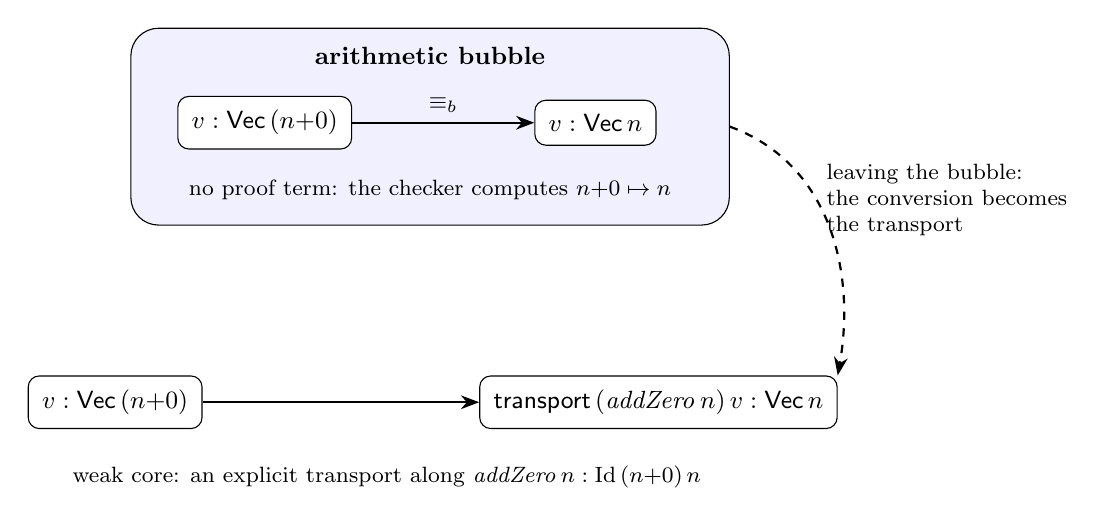
\begin{tikzpicture}[
  box/.style={draw, rounded corners, align=center, font=\small, inner sep=5pt},
  arr/.style={-{Stealth}, thick}]
\node[draw, rounded corners=10pt, fill=blue!6, minimum width=7.6cm,
  minimum height=2.5cm] (bub) at (0,0) {};
\node[font=\small\bfseries] at (0,0.9) {arithmetic bubble};
\node[box, fill=white] (in1) at (-2.1,0.05) {$v : \mathsf{Vec}\,(n{+}0)$};
\node[box, fill=white] (in2) at (2.1,0.05) {$v : \mathsf{Vec}\,n$};
\draw[arr] (in1) -- node[above, font=\footnotesize] {$\equiv_b$} (in2);
\node[font=\footnotesize] at (0,-0.8) {no proof term: the checker computes
  $n{+}0 \mapsto n$};
\node[box] (out1) at (-4.0,-3.5) {$v : \mathsf{Vec}\,(n{+}0)$};
\node[box] (out2) at (2.9,-3.5) {$\mathsf{transport}\,(\mathit{addZero}\,n)\,v :
  \mathsf{Vec}\,n$};
\draw[arr] (out1) -- (out2);
\node[font=\footnotesize, align=center] at (-0.55,-4.45) {weak core: an
  explicit transport along $\mathit{addZero}\,n : \mathrm{Id}\,(n{+}0)\,n$};
\draw[arr, dashed] (bub.east) to[out=-20, in=80] node[right, pos=0.4,
  font=\footnotesize, align=left] {leaving the bubble:\\the conversion
  becomes\\the transport} (out2.north east);
\end{tikzpicture}
\caption{Entering and leaving an arithmetic bubble. Inside, the conversion is
free; outside, the same step is an explicit transport whose proof is the step's
justification.}
\label{fig:bubble-crossing}
\end{figure}

The arithmetic bubbles are fully characterized, positive and negative cases
included (Table~\ref{tab:vec-bubbles}). \leanname{arith} contains the two
recursion equations of addition; \leanname{arithPlus} adds the left unit
$0 + t \mapsto t$, justified by induction.

\begin{table}[ht]
\centering\small
\begin{tabular}{lccc}
\toprule
Judgment & global (weak core) & \leanname{arith} & \leanname{arithPlus}\\
\midrule
$v : \mathsf{Vec}\,(n{+}0)$ given $v : \mathsf{Vec}\,n$ & no & yes & yes\\
$v : \mathsf{Vec}\,(0{+}n)$ given $v : \mathsf{Vec}\,n$ & no & no & yes\\
$v : \mathsf{Vec}\,(n{+}1)$ given $v : \mathsf{Vec}\,n$ & no & no & no\\
\bottomrule
\end{tabular}
\caption{Which vector judgments each bubble accepts
(\leanname{vec_addZero_inside}, \leanname{vec_addZero_not_global},
\leanname{vec_zeroAdd_plus}, \leanname{vec_zeroAdd_not_arith},
\leanname{vec_succ_not_inside}). Each bubble's conversion is decided by a
normal form (\leanname{Arith.conv_iff_norm}).}
\label{tab:vec-bubbles}
\end{table}

The draft runtime realizes two bubbles. An arithmetic bubble arises when
addition is admitted with its equations in a theory space. A subset bubble
arises from \code{(hol:irrelevant F J)}, which makes all proofs of $F\,x$
definitionally equal. It is admitted only when the justification $J$ proves
$\Pi x\,p\,q.\ \mathrm{Id}\,(F\,x)\,p\,q$; an unjustified declaration is not
admitted, and its verdict is undetermined, with the reason stated. A non-degenerate control remains: the
pair $(0, p)$ is still distinct from $(2, q)$.

\subsection{Why ``weak'': the weakness order on bubbles}

Read a bubble's steps as equations, and call a congruence of the core's term
syntax in which they hold on the nose a \emph{strict model} of the bubble.
Bennett's weakness of a theory is the size of its class of models
\cite{BennettWeakestNotShortest}; Goertzel's quantale weakness generalizes the
count.

\begin{theorem}[Weakness of bubbles; proved]
\leavevmode
\begin{enumerate}[leftmargin=*]
\item A bubble's conversion is exactly what its steps entail over strict models
  (\leanname{convertible_iff_entails}).
\item One bubble has fewer strict models than another exactly when it converts
  more (\leanname{models_equations_subset_iff}); every monotone measure of
  model classes, Bennett's count included, falls as conversion grows
  (\leanname{weaknessOf_le_of_convertible}).
\item The weak core is the weakest bubble (\leanname{global_weakest}), strictly
  weaker than any bubble converting two distinct expressions
  (\leanname{models_ssubset_noSteps}).
\item The weakest bubble sufficient for a program declares exactly the
  program's conversion obligations (\leanname{isWeakestAdmissible_obligations},
  \leanname{obligationBubble_types}, \leanname{obligationBubble_weakest}).
\item Over a finite catalogue of interpretations, among bubbles correct on what
  has been observed, the chance of remaining compatible with an unknown
  exchangeable future is monotone in weakness
  (\leanname{bubble_survival_mono}, \leanname{survival_antitone_in_conversion}).
\end{enumerate}
\end{theorem}

So ``use the weakest bubble that suffices'' is the choice of the weakest
sufficient hypothesis. Three limits keep the slogan honest. A justified
bubble adds nothing to the propositional theory
(\leanname{justified_bubble_propositionally_invisible}): weakness lives in
the judgmental layer only. The order is stated model by model, and may vanish
up to weak equivalence of models \cite{BocquetCoherence,OttenSpadettoPathCategories}.
The obligation bubble is not stable under substitution
(\leanname{obligation_not_substitution_stable}).

\begin{remark}[Names]
``Weak Type Theory'' already names an unrelated system for mathematical
vernacular \cite{KamareddineNederpeltWTT}, and theories with no judgmental
computation are called objective or axiomatic type theories. The settled name
here is \emph{bubble type theory} (or \emph{fibered type theory}), with
\emph{weak core} for the global layer, which is exactly the layer the theorem
above shows to be weakest.
\end{remark}

\begin{remark}[Prior art]
Varying judgmental equality by modal classification goes back to Pfenning's
intensional, extensional and irrelevant modes \cite{PfenningIntensionalityLICS}.
Multimodal type theory varies context structure per mode, but every mode keeps
the same conversion \cite{GratzerKavvosNuytsBirkedalMTT}; the extension needed
here makes $\beta$ and $\eta$ mode-indexed and adds an identity former as the
global target. The closest theorem for the crossing discipline translates
rewrite rules into axioms and conversion into transport, conservatively
\cite{BlotDowekTraversieWinterhalter}. Two-level type theory and observational
equality are candidate bubbles of the same kind
\cite{AltenkirchCapriottiKraus2LTT,AltenkirchMcBrideOTT}.
\end{remark}

\subsection{Least sufficient bubbles and the meet-closed (Horn) fiber}

When does a request have a single canonical \emph{least} sufficient bubble above
every seed? In general it does not
(\leanname{SufficientBubbles.no_least_sufficient_bubble}): conversion-preserving
and evaluation-based typing requests can admit incomparable minimal bubbles
(\leanname{ComputationBubbles.syntactic_not_convex},
\leanname{ComputationBubbles.evaluation_no_least}), and minimal inclusion can
disagree with minimal checking cost
(\leanname{CertificateBubbles.cost_inclusion_disagree}).

\begin{theorem}[Meet-closed sufficiency and the Horn fiber; proved]
Let $L$ be a complete lattice of candidate bubbles (such as $\mathcal{P}(G)$ over
a finite generator set $G$) and let $F \subseteq L$ be the bubbles sufficient
for a request.
\begin{enumerate}[leftmargin=*]
\item Seven characterizations of $F$ coincide
  (\leanname{ClosureSystems.tfae_mooreFamily}): (a)~$F$ is closed under
  arbitrary meets; (b)~$F$ is the set of closed elements of a closure operator;
  (c)~$F$ is the set of prefixed points of a monotone operator; (d)~$F$ is the
  set of elements respecting a family of implications $a \le x \to b \le x$;
  (e)~the inclusion of $F$ has a left adjoint; (f)~$F$ is the category of
  Eilenberg--Moore algebras of an idempotent monad on $L$; and (g)~every seed
  has a least member of $F$ above it.
\item Over $L = \mathcal{P}(G)$, single-conclusion implications are definite
  Horn clauses: Horn is the natural, canonical finitary syntax of meet-closure
  (\leanname{models_hornTheoryOf}, Aczel's rule presentation
  \leanname{oneStep_rulesOf}, \leanname{leastAbove_iff_hornDefinable}).
\item Within any meet-closed fiber, chaotic fair iteration reaches the least
  sufficient bubble independently of rule order or search strategy
  (\leanname{ChaoticIteration.schedule_independent},
  \leanname{effectiveSteps_le_card}).
\item When meet-closure fails, the canonical object is the Smyth upper set
  $\mathord{\uparrow}F$ of sufficient bubbles ordered by reverse inclusion
  (\leanname{DisjunctiveBubbles}), which is principal if and only if a least
  sufficient bubble exists.
\end{enumerate}
\end{theorem}

Thus a meet-closed (Horn) fiber is welcomed in Prime wherever obligations are
implicational---such as declaration closure and syntax-directed typing
(\leanname{ComputationBubbles.syntactic_isLeast})---without making Horn or
depth-first clause order the global default where conversion or disjunction
breaks meet-closure.

\subsection{The normal-form fiber: where normalizing both sides decides conversion}
\label{sec:normal-form-fiber}

The $\lambda\Pi$-calculus modulo rewriting checks a conversion by reducing both
sides to normal form and comparing the results syntactically. Call a bubble,
with a set $S$ of expressions on which conversions are asked (for a typed
calculus, its typed terms), \emph{in the normal-form fiber} when this is
correct on $S$: every element of $S$ has a normal form, and two elements of $S$
are convertible exactly when their normal forms are equal
(\leanname{NormalFormDecision.DecidedOn}).

\begin{theorem}[The normal-form fiber and its boundaries; proved]
\label{thm:normal-form-fiber}
\leavevmode
\begin{enumerate}[leftmargin=*]
\item \emph{Characterization.} Conversion on $S$ is decided by normal forms
  exactly when every element of $S$ has a normal form and convertible normal
  forms of elements of $S$ are equal (\leanname{decidedOn_iff_uniqueNormalForms});
  on a set closed under steps, exactly when every element has a normal form and
  convertible elements have a common reduct
  (\leanname{decidedOn_iff_churchRosser}). Every normalization strategy then
  computes the same normal form (\leanname{DecidedOn.normalForm_unique}).
\item \emph{Confluent and orthogonal theories.} For a confluent theory of the
  $\lambda\Pi$-calculus modulo, in particular for an orthogonal one, the fiber
  is exactly where reduction normalizes
  (\leanname{decidedOn_iff_weaklyNormalizingOn_of_orthogonal}). Orthogonality
  does not suffice: the single rule $\mathit{add}\,x\,y \hookrightarrow
  \mathit{add}\,y\,x$ passes the orthogonality test and $\mathit{add}\,x\,y$
  has no normal form (\leanname{orthogonal_not_in_fiber}).
\item \emph{An inhabitant.} Under the recursion rules of addition, conversion of
  closed arithmetic expressions is decided by normal forms
  (\leanname{PeanoFiber.peano_decidedOn}), while $x+y$ and $y+x$ are distinct
  normal terms (\leanname{plus_comm_not_conv}).
\item \emph{Nondeterminism.} With $\mathit{choose}\,x\,y \hookrightarrow x$ and
  $\mathit{choose}\,x\,y \hookrightarrow y$, the term $\mathit{choose}\,x\,y$
  has two normal forms, and no set containing it is in the fiber
  (\leanname{withChoice_not_decidedOn}).
\item \emph{Identified variables.} In a theory whose rules are headed by
  constants, variables are normal, so a conversion that identifies two distinct
  variables, as proof irrelevance does, or a variable with its
  $\eta$-expansion, is outside the fiber on every set containing them
  (\leanname{not_decidedOn_of_conv_vars}, \leanname{not_decidedOn_of_conv_eta}).
\item \emph{Symmetry.} A map of terms that carries steps to steps, with a left
  inverse that also does, sends normal forms to normal forms. So a conversion
  class that such a map preserves, with no member fixed by it, is outside the
  fiber for every relation the map respects
  (\leanname{not_decidedOn_of_symmetric_class}). Hence in every theory with
  closed definitions that converts $f\,x\,y$ with $f\,y\,x$ and keeps $f\,u\,x$
  apart from $f\,v\,x$, no set containing $f\,x\,y$ and $f\,y\,x$ is in the
  fiber, whatever the rules; under confluence $f\,x\,y$ has no normal form at
  all (\leanname{not_decidedOn_of_commutative},
  \leanname{no_normalForm_of_commutative}).
\end{enumerate}
\end{theorem}

Items~1 and~2 are classical \cite{NewmanCombinatorial,HuetConfluentReductions,KlopCRS},
and so is the commutative case of item~6: commutativity cannot be oriented,
which is why rewriting modulo associativity and commutativity was introduced
\cite{PetersonStickelAC,JouannaudKirchnerModulo}. Item~6 is stated in the form
used here, where the symmetry is a renaming of variables.

\paragraph{Definability.}
The meet-closed fiber has its definability theorem: the Horn-definable families
are exactly the intersection-closed ones (\leanname{leastAbove_iff_hornDefinable}).
The normal-form fiber has one too, over any term structure whose one-hole
contexts compose and whose substitutions enter contexts uniformly. An
equivalence is the conversion of rule schemas whose normal forms decide it on
every term exactly when it is closed under contexts and substitutions and has
a transversal, one representative per class, that is closed under subterms and
reflects substitution instances (\leanname{SchematicPresentation.exists_presentation_iff}).
The representatives are then the normal forms
(\leanname{normalForms_of_presentation}), and conversely the rules
$\sigma(s) \mapsto \sigma(\mathrm{rep}\,s)$ present the equivalence
(\leanname{presentation_of_transversal}); the rule set is infinite in general.
On binary terms, associativity has such a transversal, the right-nested terms
(\leanname{assoc_presentation}), and commutativity has none
(\leanname{commEq_no_presentation}). Whether a finite presentation exists is a
further question, on which a finitely presented theory with decidable word
problem may still have no finite convergent presentation
\cite{SquierFiniteDerivationType}; that boundary is not formalized here, nor is
the version of the theorem for normalization asked only on typed terms.

\paragraph{The operational reading.}
The GSLT of a step relation has a native OSLF type that observes undirected
conversion (\leanname{satisfies_conversionNativeType_iff}). On a set in the
normal-form fiber, that observation holds between two terms exactly when the
normal forms computed by the directed steps are equal
(\leanname{satisfies_conversionNativeType_iff_normalForm_eq}); for the recursion
rules of addition it relates $2+3$ with $5$ and not with $4$
(\leanname{peano_oslf_two_plus_three}). Outside the fiber the observation keeps
its meaning, but running the steps does not decide it.

\paragraph{The fiber in the bubble order.}
A bubble declared by rule schemas is closed under substitution and under the
exchange of two variables (\leanname{BubbleSchematic.Schematic}). The weakest
schematic bubble meeting a set of required conversions is their closure under
both operations (\leanname{schematicClosure_weakest}), and that closure is the
least model of a Horn theory with one-premise clauses
(\leanname{schematicClosure_eq_hornClosure}); for a program, it is the weakest
schematic bubble typing the program (\leanname{schematicObligation_weakest}).
So the meet-closed fiber computes the weakest schematic bubble, and the
normal-form fiber says when normalizing decides it. For the program that uses
$v : \mathrm{Vec}\,(x+y)$ at $\mathrm{Vec}\,(y+x)$, every schematic bubble that
types it and keeps $\mathrm{Vec}\,(x+x)$ apart from $\mathrm{Vec}\,(x+y)$ is
outside the normal-form fiber on the program's two types
(\leanname{CommutationProgram.schematic_not_decidedOn}); its weakest schematic
bubble and the bubble declaring commutativity of every sum are two such bubbles
(\leanname{weakest_not_decidedOn}, \leanname{commAdd_not_decidedOn}).
Presenting a bubble by directed rules costs no strict model: strict models
depend only on conversion, and reversing every declared step changes neither
(\leanname{models_eq_of_convertible_iff}, \leanname{models_flip}).

\paragraph{The neighbouring routes.}
Each boundary has a route that decides what normalizing both sides cannot.
\begin{itemize}[leftmargin=*]
\item \emph{Comparison up to a built-in equivalence}, as in rewriting modulo
  associativity and commutativity. Deciding by normal forms is the case of
  syntactic equality (\leanname{decidedOn_iff_decidedModuloOn_eq}); with
  commutativity built into the comparison, commutativity is decided with
  equivariant data (\leanname{CommutativeTerms.decidedModuloOn_commEq}), and
  commutativity itself is decided by sorted forms
  (\leanname{commEq_iff_sortForm_eq}).
\item \emph{Ordered rewriting, or variables as codes.} Orienting a commutation
  only when it lowers a fixed numbering of terms decides commutativity by normal
  forms (\leanname{orderedStep_decidedOn}) and is not equivariant
  (\leanname{orderedStep_not_equivariant}) \cite{MartinNipkowOrdered}. An
  encoding of universe levels whose variables are closed codes is of this kind:
  its conversion on level codes is equality of computed normal sets
  (\leanname{conv_code_iff_normalSet}). An encoding that keeps the level
  variables builds commutativity into matching \cite{GenestierAgda}.
\item \emph{Type-directed conversion} for $\eta$ and proof irrelevance
  \cite{CoquandConversion,GilbertProofIrrelevance}.
\item \emph{Explicit steps.} The weak core is in the fiber trivially, with
  conversion syntactic identity (\leanname{noSteps_decidedOn}); each step is then
  paid for in the certificate (\leanname{size_discardTower}).
\item \emph{The running GSLT} hosts nondeterminism, which no confluent theory
  hosts (\leanname{withChoice_not_hosted_by_confluent}); cyclic values need
  bisimulation, since no theory that terminates on typed terms reads hyperset
  membership as reduction (\leanname{no_typed_reading_of_membership}).
\end{itemize}
On commutativity the first two routes are theorems where normalizing both sides
fails; a comparison of the routes on a common measure of cost is not
formalized.

\paragraph{Translations.}
A translation into the $\lambda\Pi$-calculus modulo lets its checker decide the
source's conversion under three obligations: it preserves conversion, it
reflects conversion, and its image lies in the normal-form fiber
(\leanname{DecidedOn.transport}). A translation that carries steps to
reductions carries normalization of the source to the image of a confluent
target (\leanname{decidedOn_image_of_simulation}). For the embedding of pure
type systems \cite{CousineauDowekPTS} the first two are theorems
(\leanname{translate_conv}; \leanname{translate_reflects}, up to the erasure of
annotations), the theory of the embedding is confluent, and the third reduces
to weak normalization of the translations (\leanname{cd_decidedOn_iff},
\leanname{cd_transport}); that normalization is not formalized here.

For higher-order logic the three obligations are discharged end to end. The
source is the intrinsically typed higher-order logic of the tree, with many
sorts, constants, the connectives, equality and both quantifiers, and with
$\beta$ at every position, which normalizes strongly and is confluent. An
encoding names the symbols injectively and translates a term shallowly, with
the decoding of its type's code as the domain of each abstraction. Take a
confluent theory with headed rules that defines none of the named symbols and
in which the decoding of a code reduces to a product of normal decodings of
named codes. There every $\beta$-step of the source is a step of the target
(\leanname{translate_betaStep}). The translation of a source normal form,
with its domains computed, is normal and injective. So every translated term
has a normal form, the checker decides conversion by normal forms on the
translated terms (\leanname{decidedOn_translations}), and two terms are
$\beta$-convertible exactly when their translations are convertible
(\leanname{translate_conv_iff}). Weak normalization of the image is carried
from the strong normalization of the source by the simulation; normalization
of the target on the terms it types is not used. The encoding of
\cite{AssafBurelHOL} is such a theory (\leanname{holideHub}), and so is the
hub of \cite{DowekThireLogipedia} (\leanname{sttfaHub}). Its six rules are
transcribed from its theory file (Logipedia, \texttt{theories/sttfa/sttfa.dk}
at commit \texttt{0bcb193}), where $\mathtt{eta}$ is a defined symbol,
$\mathtt{eta} \longrightarrow \lambda t.\,\mathtt{etap}\,(\mathtt{p}\,t)$,
and pass the orthogonality test (\leanname{STTfa.check}). Once the symbols of the signature are declared, the
translations are typed in both theories (\leanname{holide_translate_typed},
\leanname{sttfa_translate_typed}); the hub with proofs also declares the
remaining constants of the theory file, $\mathtt{ptype}$, $\mathtt{p}$,
$\mathtt{etap}$, $\mathtt{forallK}$, $\mathtt{eps}$ and $\mathtt{forallP}$.
The natural-deduction proofs of $\Rightarrow$
and $\forall$ modulo $\beta$ compile in the hub to terms of
$\mathtt{eps}$ of the translated conclusion (\leanname{ProofHub.theorem_typed},
\leanname{sttfa_theorem_typed}).

Conversely, on the closed implicational fragment, whose atoms are the
$\beta$-normal formulas that are neither implications nor universals, every
normal inhabitant of $\mathtt{eps}$ of a translated formula, in the context of
the types of the proofs of hypotheses of the fragment, comes from a proof
(\leanname{sttfa_adequate}). The proof is an induction on the normal term with
typing inversion; the types of objects form a class closed under the steps of
the hub that contains no normal type of a proof
(\leanname{objTree_not_conv_epsNF}). With universal quantification adequacy is
not exact. The bare connective $\mathtt{and}$ is normal and has the decoding of
the code of $\mathrm{prop}\Rightarrow\mathrm{prop}\Rightarrow\mathrm{prop}$, but
it converts with no translation, since translations apply it to two operands
and the steps of the hub keep it so, as for the code formers of
\cite{CousineauDowekPTS}. Applied to a hypothesis of $\forall f.\,P$, it gives a
normal inhabitant of $\mathtt{eps}\,P$ to which no proof compiles, although $P$
follows from the hypothesis with another witness
(\leanname{sttfa_not_exactly_adequate}). Modulo the coding of witnesses,
adequacy holds: a normal term in which every abstraction binds a hypothesis or
an object at its normal decoding, and every $\forall$-witness is the translation
of a core term, typed at $\mathtt{eps}$ of a closed core formula in the context
of the proofs of closed core hypotheses, comes from a proof
(\leanname{sttfa_adequate_coded}); so does one typed at a core formula with free
objects in the context of their decodings
(\leanname{sttfa_adequate_coded_open}). The bare-$\mathtt{and}$ witness is not
coded (\leanname{sttfa_coding_needed}). Formulas and witnesses are core because
the retyping step of the source converts core terms only. These theorems are
about normal terms: normalization of the typed terms of the hub is not proved,
so they do not yet make the hub conservative over higher-order logic. $\eta$ is
a conversion of neither theory (\leanname{eta_not_conv}).

A reading of a signature in a package of proposition codes reads the core of
the same source (variables, interpreted constants, application, abstraction,
$\Rightarrow$, $\forall$ and equality). On read terms, convertible
translations in a hub have equal reads in every lawful reading
(\leanname{fiber_equal_of_conv}). The converse fails at $\eta$: the reads of
$\lambda x.\,f\,x$ and $f$ are equal in every lawful reading, and their
translations are convertible in no hub (\leanname{fiber_not_conservative}).
On read terms, $\beta\eta$-conversion of the source is equality in every lawful
reading (\leanname{readBetaEta_equal}). The converse fails in general for an
expected reason: a package may interpret a constant by a rule, as the set
profile computes $\mathrm{add}\,x\,\mathrm{zero}$ to $x$, while higher-order
logic treats the constant as uninterpreted, so the reading equates terms that
are not $\beta\eta$-convertible (\leanname{set_fiber_beyond_betaEta}). Whether
equality is exactly $\beta\eta$ on read terms for packages that add no
equations between them is open; it needs a model of the package in which
$\beta\eta$ is decided algorithmically, or a set-theoretic model together with
the completeness of $\beta\eta$ for the full type hierarchy over an infinite
base \cite{FriedmanEqualityFunctionals}. For the set profile, one proof is
typed both in the hub and in the object package
(\leanname{sucProof_in_both}), and the normal form of its compiled term gives
the proof back (\leanname{set_sucProof_adequate}).

A translation whose source has a
commutative definitional equality on variables, such as $\max$ on universe
levels, lands outside the fiber unless it builds commutativity into matching or
encodes the variables as codes \cite{GenestierAgda,BlanquiVaishnavLean}.

\subsection{The empty top and the inconsistent-top method}

In the theory--model Galois connection, the theory of all sentences is the
top. Under classical satisfaction it has no model. If the candidate structures
include a degenerate one, a structure where everything holds, then that
structure is the top's only model, and no axiom can carve it away: excluding it
means choosing a different universe of structures. The model that is actually
useful sits between the two: a \emph{permissive} model in which every type is
inhabited while conversion stays non-degenerate.

The same picture gives a method for metatheory. Syntactic properties such as
$\Pi$-injectivity and subject reduction do not need consistency, so they can be
proved for a maximally permissive, even inconsistent, theory with a universe
$U : U$ through a domain-theoretic model \cite{CoquandDomainSemantics}. The
method has been ported to Lean's own theory \cite{CarneiroLean4Lean}. For Prime
its contract is: separations transfer to every carved fragment; closure results
such as subject reduction transfer only along a conservative embedding;
consistency and normalization never transfer, and each fragment needs its own
model with an empty type.

\subsection{Hosted logics and translations between them}

\begin{table}[ht]
\centering\small
\begin{tabular}{>{\raggedright\arraybackslash}p{2.6cm}
  >{\raggedright\arraybackslash}p{5.2cm}
  >{\raggedright\arraybackslash}p{5.2cm}}
\toprule
Layer & What varies & What a crossing carries\\
\midrule
Conversion bubbles & which computations count as definitional equality,
  within shared judgments & a justification for each step; substitution and
  transport laws\\
Different logics & judgments, equality, rules, axioms and models & an explicit
  interpretation that states what it preserves\\
Operational regions & machines, representations, scheduling, observation &
  preservation of the declared observable behaviour\\
\bottomrule
\end{tabular}
\caption{Three layers, three crossing contracts.}
\label{tab:three-layers}
\end{table}

A host must preserve the distinctions and counterexamples of its guest, not
only its truths, and must advertise any commitment it adds. The requirement is
not cosmetic: a host can preserve every truth of a guest and still create new
ones when its interpretation represents too few guest models
(\leanname{InstitutionBridge}). The institution machinery makes the
requirement checkable \cite{GoguenBurstallInstitutions}.

\begin{theorem}[Hosting; proved]
\leavevmode
\begin{enumerate}[leftmargin=*]
\item A logic graph flattens into its Grothendieck institution, with a
  canonical comorphism from each node that preserves and reflects entailment
  (\leanname{GrothendieckInstitution}) \cite{DiaconescuGrothendieckInstitutions}.
\item For a sound and complete target, borrowing its prover through a
  comorphism is sound exactly when the comorphism is conservative
  (\leanname{borrow_sound_iff_conservative}) \cite{CerioliMeseguerBorrow};
  borrowing along a collapsing translation derives a true conclusion from
  false premises (\leanname{Control.collapse_borrows_false_conclusion}).
\item Proof-carrying routes compose, and certificates return only along
  conservative routes (\leanname{TheoryGraphProofTransport}).
\item Route choice prefers a conservative route, then the route adding the
  fewest commitments, then the weakest; two optimal routes can be
  incomparable (\leanname{Control.incomparable_optima}).
\end{enumerate}
\end{theorem}

The native higher-order logic has its own namespace. A theory space selects
the logic alone with \code{(hol:profile base)} and is judged with \code{hol:}.
Its metatheory is anchored in two proved packages:
\begin{itemize}[leftmargin=*]
\item \textbf{Classical HOL and Farmer's seven virtues}
  (\leanname{SevenVirtues}): Church-style extensional HOL with a single
  excluded-middle axiom $\forall p.\, p \lor \neg p$ is sound and Henkin-complete
  for countable signatures with closed sort inhabitants
  (\leanname{SevenVirtues.Completeness.provable_iff_valid},
  \leanname{consistent_iff_satisfiable}), categorical for second-order Peano
  arithmetic (\leanname{Peano.categorical}) and complete ordered fields
  (\leanname{OrderedField.categorical}), and strictly separated from Hilbert's
  choice operator $\varepsilon$ by a Fraenkel--Mostowski permutation model
  (\leanname{Choice.choice_separates}).
\item \textbf{Intuitionistic HOL} (\leanname{HeytingGeneral}): parameter-free
  theories are sound and complete for Heyting-valued substitutional models
  (\leanname{provable_iff_heytingConsequence_param_free}).
\end{itemize}
Tier-0 grounding follows \emph{correct-by-construction} (Rung~1): minimal HOL
proves the candidate or native-inference checker faithful once, while
per-run certificates and translations to HOL Light, Megalodon and MM0
(\code{hol.mm0}) serve as interop and acceleration bridges checking the same
fiber semantics.
Every set theory is a set profile over that base logic and is judged with
\code{set:}: the shared material fragment by default, and the set theory HOTG,
HOL with set axioms, selected with \code{(set:profile megalodon-hotg)}, never by
default \cite{BrownKaliszykPakHOTG}. A set profile's signature includes the
base logic's declarations and rules, and \code{(set:signature base-logic)}
answers \code{(hol:profile base)}. The hosted HOL Light kernel keeps its own
operations under \code{hol-light:}. Figure~\ref{fig:hol-set-routes} shows the
routes between them that run today.

\begin{figure}[ht]
\centering
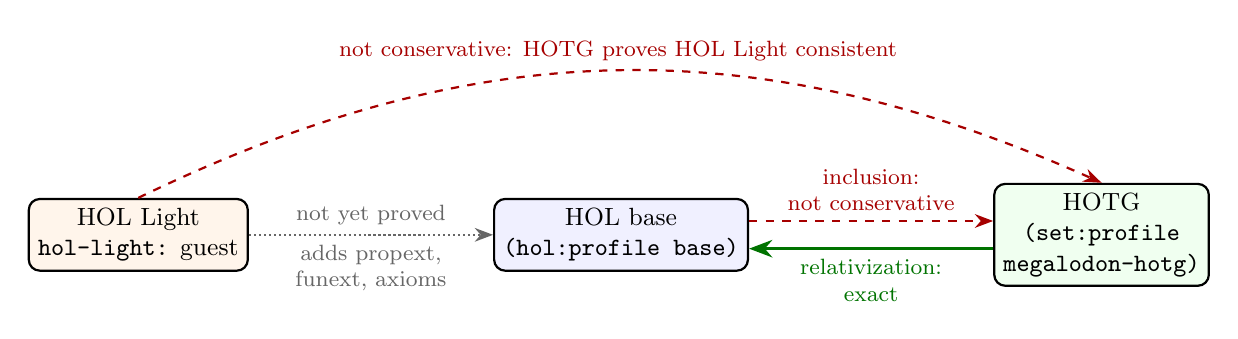
\begin{tikzpicture}[
  node distance=3.1cm,
  logic/.style={draw, rounded corners, thick, align=center, font=\small,
    minimum width=2.6cm, minimum height=0.9cm},
  cons/.style={-{Stealth}, very thick, green!45!black},
  ncons/.style={-{Stealth}, thick, red!65!black, dashed},
  unk/.style={-{Stealth}, thick, black!60, densely dotted}]
\node[logic, fill=orange!8] (hl) {HOL Light\\\code{hol-light:} guest};
\node[logic, fill=blue!6, right=of hl] (base) {HOL base\\\code{(hol:profile base)}};
\node[logic, fill=green!6, right=of base] (hotg) {HOTG\\\code{(set:profile}\\\code{megalodon-hotg)}};
\draw[unk] (hl) -- node[above, font=\footnotesize] {not yet proved}
  node[below, font=\footnotesize, align=center] {adds propext,\\funext,
  axioms} (base);
\draw[ncons] (hl.north) to[bend left=25] node[above, font=\footnotesize]
  {not conservative: HOTG proves HOL Light consistent} (hotg.north);
\draw[ncons] ([yshift=5pt]base.east) -- node[above, font=\footnotesize,
  align=center] {inclusion:\\not conservative} ([yshift=5pt]hotg.west);
\draw[cons] ([yshift=-5pt]hotg.west) -- node[below, font=\footnotesize,
  align=center] {relativization:\\exact} ([yshift=-5pt]base.east);
\end{tikzpicture}
\caption{Routes between HOL and set theory that run in the draft runtime.
Solid: conservative (proved). Dashed: not conservative, with the added
commitments named. Dotted: conservativity not yet proved.}
\label{fig:hol-set-routes}
\end{figure}

The same judgments are importable from the other dialects: \code{import hol}
and \code{import set} give Prime, HE and PeTTa programs the judgments of the
logic and of its set theories, each over an explicit theory space and with
answers returned as data. The HOL Light guest is not
offered in HE until a translation into HE is qualified.

\subsection{HE's types grounded in HOL}

HE's types can mention symbols that also name terms: its own tests type
length-indexed vectors with \code{(: Cons (-> \$t (Vec \$t \$x) (Vec \$t (S \$x))))}.
The indices are matched by syntactic unification. HE has no binder that names an
argument, so \code{(: remember (-> Fact (WitnessOf \$p)))} gives
\code{(remember fact)} the type \code{(WitnessOf \$p)} for every \code{\$p};
and it has no conversion, so \code{(Vec Nat (plusZ Z))} does not match
\code{(Vec Nat Z)} even when \code{(plusZ \$n)} reduces to \code{\$n}. Read as
propositions, HE's types are all inhabited: \code{if} has the type
\code{(-> Bool Atom Atom \$t)}, so \code{(if True Z Z)} is accepted wherever any
type is expected, including a declared type with no constructors. This is the
situation of a programming language with general recursion, not a paradox:
\code{Type} itself has the unknown type \code{\%Undefined\%}, not \code{Type}.
Statically accepted terms are checked again at run time; \code{(needEmpty (if
True Z Z))}, with \code{needEmpty} expecting the constructor-free type
\code{Empty}, is accepted statically and evaluates to
\code{(Error Z (BadType Empty Nat))}, as gradual typing prescribes.

On a fragment, HE's checker is one well-defined typing relation, and each such
fragment is exactly HOL typing, where every type denotes a non-empty set and the
truth of a proposition is a theorem of type \code{bool}, not the inhabitation of
a type: saturated applications of declared static arrows
(\leanname{hol_iff_exact}), type variables as polymorphic constants with HE's
answer as the principal scheme (\leanname{Schematic.schematic_hol_iff_exact}),
tuples as products (\leanname{Tuples.reference_iff_tupleHOLTyped}), meta-types
as a classification theory (\leanname{MetaTypes.metaAccepts_iff_entailed}), and
\code{\%Undefined\%} as the unknown type of abstract gradual typing
(\leanname{Gradual.corePlusR2Consistent_iff_top}) \cite{GarciaClarkTanterAGT}.
Furthermore, the first-order HOL typing contract is proved to agree across all
three native kernel realizations---HOL Light, Megalodon
(\leanname{MathdataKernel.inferTerm}) and MM0 (\leanname{Preterm.infer})
(\leanname{KernelRealizations}).
At run time Prime answers HE-style declarations inside these fragments from the
hosted HOL Light checker, never HE's type engine; a Prime candidate may
implement that contract only as a replaceable backend with proved
correspondence. A failed check inside the
fragments is a genuine refutation; outside them the answer is undetermined and
never a reason to prune an alternative.

The \code{he-prime} profile extends HE with named binders, as in
\code{(-> (: \$p Fact) (WitnessOf \$p))}, for which upstream HE gives no type.
These are genuinely dependent and lie outside every simple fragment. The proposed treatment is a stable $\lambda\Pi$
contract, of which the HOL contract is the simple slice, checked by a hosted
logical-framework kernel. Until then such declarations are left undetermined.

\subsection{Demand, sharing and effects}
\label{sec:demand-effects}

The operational contract requires that a shared value be computed once, that an
effect happen once, and that a bounded observation bound both work and effects.
Figure~\ref{fig:select-timeline} contrasts an eager and a bounded run of
\code{(select 2 (gen))}, where each of four alternatives writes an atom before
answering.

\begin{figure}[ht]
\centering
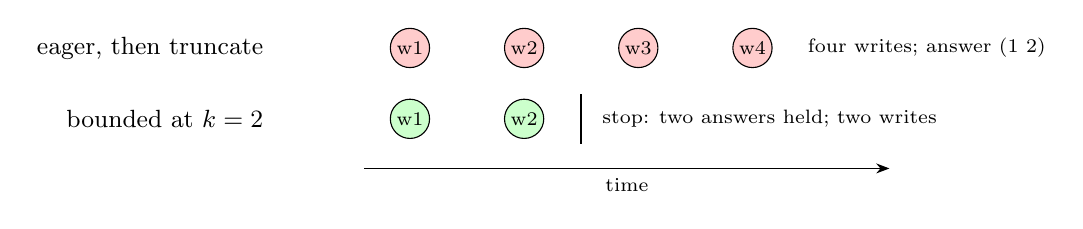
\begin{tikzpicture}[x=1.45cm, y=0.9cm,
  ev/.style={circle, draw, inner sep=1.3pt, font=\scriptsize},
  lab/.style={font=\small, anchor=east}]
\node[lab] at (-0.2,1) {eager, then truncate};
\node[lab] at (-0.2,0) {bounded at $k=2$};
\foreach \i in {1,...,4} {
  \node[ev, fill=red!20] (e\i) at (\i,1) {w\i};
}
\node[font=\scriptsize, right] at (4.4,1) {four writes; answer $(1\ 2)$};
\foreach \i in {1,2} {
  \node[ev, fill=green!20] (b\i) at (\i,0) {w\i};
}
\draw[thick] (2.5,-0.35) -- (2.5,0.35);
\node[font=\scriptsize, right] at (2.6,0) {stop: two answers held; two writes};
\draw[-{Stealth}] (0.6,-0.7) -- node[below, font=\scriptsize] {time} (5.2,-0.7);
\end{tikzpicture}
\caption{Bounded selection in the illustrated sequential policy. The run stops
at its $k$-th successful answer and avoids later effects. An infinite producer
must reach those successes in finite work for this observation to terminate.}
\label{fig:select-timeline}
\end{figure}

Three runtime defects of this kind were found and removed in the draft runtime.
Each now has a route-agreement fixture, so the default route, the reference
route and the fuel-bounded evaluator must agree, and each has a mutation that
reintroduces it and is killed:
\begin{enumerate}[leftmargin=*]
\item selection of $k \ge 2$ answers ran every alternative's effects before
  truncating, and did not terminate on infinite producers
  (\leanname{bounded_selection_stop}, \leanname{bounded_selection_effects});
\item a shared pending value reaching two strict operands of a primitive was
  computed twice (\leanname{strict_operand_sharing});
\item a binding whose closed source produced no answer ran that source twice
  (\leanname{empty_source_once}).
\end{enumerate}
Retained search must distinguish a snapshot continuation from validated-fresh
resumption. The latter checks the dependencies of already performed reads;
an unrelated write need not invalidate them, while a changed complete result
or absence must not reuse the old answer. Stateful own writes require their
own continuation law. Section~\ref{sec:execution-contracts} establishes the
pure adaptive-query join; the complete effectful retained-world and native
resumption comparison remains an implementation obligation.

\paragraph{Answers, choice and probability.}
The speculative layer is read through weighted answers,
$\mathsf{Spec}\,K\,C\,W\,X=W\to\mathsf{Ans}_K(X\times W\times C)$, which aggregate
equal outcomes, forget their order and drop branches without answers together
with their cost.  This readout is an observer of ordered runs, not a
replacement for them: an ordered run returns its branch outcomes in order, and
a failed branch keeps its world and the cost it paid.  Observing a sequenced
run is sequencing the observations, so the observer is a monad morphism
(\leanname{SpecRunObserver.observe_pure}, \leanname{observe_bind}); it forgets
order and the cost of failed branches (\leanname{Controls.observe_forgets_order},
\leanname{Controls.observe_forgets_failed_cost}).  Laws proved for
$\mathsf{Spec}$ are laws of what ordered runs show through this observer.

Nondeterministic choice and probability are distinct effects.  No distributive
law of finite distributions over finite sets exists
\cite{VaraccaWinskelDistributing,ZwartMarsdenNoGo}
(\leanname{NondeterminismProbability.no_distributiveLaw}); in one weighted
monad, additive choice and convex probabilistic choice are both algebraic, and
the support readout identifies them
(\leanname{convex_bind}, \leanname{support_convex}).  Probability becomes a view
of a program with choice only once a scheduler resolves each choice.  Without
choice every scheduler gives the same probabilities
(\leanname{SchedulerResolution.prob_choiceFree}); with choice, the envelope of
probabilities over all randomizing schedulers is attained by deterministic
ones (\leanname{exists_deterministic_le}, \leanname{exists_deterministic_ge}),
so the honest view is the convex set of distributions between those extreme
points, the convex powerset of mixed powerdomains
\cite{KeimelPlotkinMixed}.  A pure choice between two outcomes has every
probability in $[0,1]$ (\leanname{choice_probabilities}), the interval readout
of zero evidence.  Counting paths is one scheduler among many: normalizing the
additive readout of a three-way choice built from two binary choices gives
$1/3$, fair coins give $1/2$, and the scheduler weighting each choice by its
number of paths gives $1/3$ (\leanname{Controls.counting_not_fair}).  Evidence
weights differ from both: they count observations, probabilities sum to one,
and a nondeterministic choice carries no weight at all.

\paragraph{Where each element lives.}
The theorems above fix where each element belongs in a theoretical Prime,
without selecting a candidate calculus.  A \emph{primitive} cannot be
recovered from the others; a \emph{library} is defined over primitives with
the laws it needs; a \emph{profile} is a declared choice of strategy or
semantics that consumers can rely on.
{\small
\begin{longtable}{>{\raggedright\arraybackslash}p{0.16\linewidth}%
                  >{\raggedright\arraybackslash}p{0.10\linewidth}%
                  >{\raggedright\arraybackslash}p{0.31\linewidth}%
                  >{\raggedright\arraybackslash}p{0.29\linewidth}}
\toprule
Element & Place & Typing and authority & Justifying theorem \\
\midrule
\endhead
Annotated space and weighted answers & primitive & one semiring per space,
  with declared capabilities (merge; meet, monus and join where they exist) &
  \leanname{Ans.bind_assoc}, \leanname{support_bind_iff_positive},
  \leanname{no_space_sub_undoes_merge} \\
Evidence algebra & library & counts as a positive annotation; ledgers carry
  identities; revision of overlapping ledgers is typed by a disjointness proof
  or falls back to the maximum; readouts return ``undetermined'' &
  \leanname{additive_revision_exact_iff_disjoint},
  \leanname{unknown_overlap_bounds}, \leanname{conjunction_counts_iff} \\
Absence at frontiers & primitive guard & an absence read carries its
  certificate, the owner of the pattern's head and the frozen rule set; only
  the owner revokes & \leanname{knot_iff_absent_frontier},
  \leanname{ownership_certifies_frontier}, \leanname{foreign_extension_certified} \\
Call & primitive step & a synchronous call is a step of the kernel, not
  sugar over rewriting & \leanname{call_not_locally_eliminable} \\
Seals and owned namespaces & primitive & sealing and the right to extend a
  head are capabilities; kernels resolve helpers in a closed environment &
  \leanname{isEmpty_sealElimination}, \leanname{late_bound_forgery},
  \leanname{owned_sound} \\
Consumption & primitive step, arbitration by profile & the consume right is
  exclusive; commit order, optimistic validation or exclusive authority
  arbitrates & \leanname{consumption_not_confluent},
  \leanname{first_committer_wins}, \leanname{gated_confluent} \\
Strategy & profile & priority keys are semantic; a fairness certificate is an
  overtaking bound, realized by deadlines or epochs &
  \leanname{priority_not_weakly_fair}, \leanname{fires_within_overtaking},
  \leanname{deadline_fires_within} \\
Probability and choice & library and readout & probability is an annotation;
  credal sets are the readout of choice under all schedulers &
  \leanname{no_distributiveLaw}, \leanname{exists_deterministic_le},
  \leanname{choice_probabilities} \\
Knowledge-based programs & library & three-valued tests answered by grounded
  inquiry; ranked programs are decided & \leanname{stage_sound},
  \leanname{least_decides} \\
Observer-indexed truth & library & knowledge is the interior of an observer's
  partition & \leanname{knows_le}, \leanname{knows_knows} \\
Speculative readout & observer & $\mathsf{Spec}$ observes ordered runs; order
  and paid work stay with the runs & \leanname{observe_bind},
  \leanname{Controls.observe_forgets_failed_cost} \\
\bottomrule
\end{longtable}
}

\subsection{Open decisions}

\begin{enumerate}[leftmargin=*]
\item The stable $\lambda\Pi$ contract for dependent HE declarations, and the
  hosted kernel that checks it.
\item Pairing conversion bubbles (\leanname{BubbleWeakness}) with axiomatic
  little-theory nodes (\leanname{HenkinInstitution}), cross-base feature
  composition, and the weakness order for full models of type theory rather
  than term congruences.
\item Generic derivation of the complete dependent eliminator from an authored
  inductive signature across the indexed-polynomial container spine
  (\leanname{IndexedPolynomial}) and proof-relevant $\iota$ conversion policies
  (\leanname{ConversionRecipes.Policy}).
\item Full Kripke--Henkin completeness for intuitionistic HOL via a scheduler
  provider extending the proved Heyting substitutional completeness
  (\leanname{HeytingGeneral}).
\item Bounded \code{select} and \code{once} in HE's extended profiles, and
  eliminating any fixed implementation bound on contextual frame identities in
  the runtime.
\end{enumerate}

\section{Prime's planned CBPV basis and qualified evaluation strategies}

The intended next foundation for Prime is CBPV-based, with a theoretically
qualified mixture of eager evaluation, suspension and sharing. This is a
design direction, not a completed migration or a choice of every surface
default. The current Prime nucleus includes a call-by-need layer: computation
is demanded when required, and subsequent uses of the same qualified need
cell reuse its cached outcome. Ownership, revision and occurrence identity
determine which uses may share that cell.

Call-by-push-value (CBPV) distinguishes value types from computation types and
relates them through the familiar $F\dashv U$ organization. Call-by-name (CBN)
and call-by-value (CBV) arise as translations into this common
value/computation language \cite{LevyCBPV}. Plain thunk/force does not itself
memoize a result. McDermott and Mycroft extend CBPV with a need binder and
effect-sensitive equations for evaluation-order reasoning
\cite{McDermottMycroftExtendedCBPV}. This is a candidate construction to
compare with Prime's existing need protocol, not an automatically adopted
calculus. A strict primitive, guest calculus or optimized fragment must
preserve its declared observation and surrounding demand/sharing contract;
the existence of a CBV or CBN translation is not permission to change it.

For example, eagerly evaluating an unused diverging argument changes
termination; rerunning a shared nondeterministic choice can change a correlated
pair into two independent results; moving a read across a write can change
its value. The permitted rewrite therefore depends on demand, effects and
the observer. Effect/coeffect tracking offers a way to certify both effects
and variable-use requirements \cite{TorczonEffectsCoeffects}; it is not a
proof that any one strategy minimizes total cost. A proposed optimization
must separately establish semantic preservation and its cost advantage on
the advertised workload.

\nolinkurl{ContextualStrategyQualification} supplies a first general law for
the existing contextual-effect syntax, without introducing another evaluator.
A structurally read-only program---no choice, write or intent---can be
evaluated once and its value reused in place of two consecutive evaluations
before any effectful continuation. It can also be discarded when unused.
The proof preserves the isolated-world evaluator's complete ordered result:
branch paths, answers, final states and intent lists. Its observation does
not count reads, so this is not a work or full-trace equality theorem.
The controls distinguish independent Boolean choices from a correlated reused
choice, equal answer support with four versus two result occurrences, repeated
state increments, and repeated deferred intents. Even equal answer support
does not permit changing multiplicity. These are sufficient qualification
laws at demanded sites, not a general need implementation, a necessary
criterion, or a result about divergent computations.

The value/computation boundary now has a concrete semantic instance in
\nolinkurl{ContextualKleisliAdjunction}. For the existing contextual program
monad $T$, the existing Kleisli category supplies
\[
  F:\mathbf{Type}\rightleftarrows\mathbf{Kl}(T):U,
  \qquad F\dashv U,
  \qquad U(B)=\mathsf{Program}(S,|B|,I).
\]
Here $F$ sends a value map to pure return; $U$ acts on an arrow by sequencing
with its program. In particular, $U$ does not simply extract an answer type.
The natural hom equivalence and both triangle laws are checked, and the
induced monad's multiplication is the existing \texttt{bind}, not a new
evaluator. A real choice is outside the pure unit's image. This is a Kleisli
resolution of the monad, not a complete CBPV model: computation products and
value-indexed computation function objects are not supplied by the adjunction
alone \cite{LevyAdjunctionSemantics}.
There is now a checked obstruction, not merely missing infrastructure:
\nolinkurl{ContextualKleisliProductBoundary} proves that the singleton-state,
singleton-intent instance has no terminal computation object. Every program
has a positive finite answer-occurrence count, and duplicating it by choice
doubles that actual handler observation. Any supposed terminal target would
have to identify an arrow into it with its duplicated-choice arrow. Ordinary
value types still have their terminal singleton; applying $F$ does not make
it terminal on the computation side. The free-returner category therefore
lacks even the empty computation product. A full CBPV model needs a richer
computation category or an explicitly justified change of observation;
neither is supplied by relabeling the existing adjunction. This does not
refute every binary computation product or require erasing occurrences.

An algebra-based candidate now resolves this structural obstruction without
changing the existing programs. \nolinkurl{ContextualComputationAlgebra}
uses Mathlib's Eilenberg--Moore algebras for the same $T$, its free/forgetful
adjunction and the comparison functor
\[
  \mathbf{Kl}(T)\lhook\joinrel\longrightarrow\mathbf{Alg}(T).
\]
The comparison is fully faithful: evaluating a free-algebra homomorphism on
pure inputs recovers its original Kleisli arrow, and the homomorphism law
proves the converse. Both encodings retain literal choice/effect programs;
the new adjunction induces the same sequencing.
\nolinkurl{ContextualComputationAlgebraProducts} constructs varying-family
products by Mathlib's creation of limits. Their carriers are dependent
functions, and their actions and projections are pointwise. The empty product
is terminal, but the free returner $F1$ is not: appending an intent and doing
nothing are distinct algebra endomorphisms. This does not quotient programs
or authorize effect erasure.

\nolinkurl{ContextualAlgebraSequencing} supplies the contextual interfaces:
computations are functions from value contexts into algebra carriers;
stacks are context-indexed algebra homomorphisms. Sequencing into any target
algebra satisfies unit, associativity and stack compatibility, while a free
target recovers actual \texttt{Program.bind}. Contextual continuations
transpose to stacks from free returners. Products, value-indexed computation
functions and value coproducts have their computation/stack universal
properties, with context reindexing and resume compatibility. These are the
module-relative semantic interfaces of adjunction semantics
\cite{LevyAdjunctionSemantics}; they do not themselves reify a dependent
CBPV source language.
In particular,
\[
  F(A\to B)\quad\hbox{and}\quad A\to F B
\]
are different interfaces: an argument-dependent intent lies outside the
canonical map from computations returning pure functions.

The distinction reaches a real mathematical consumer in
\nolinkurl{NativeConversionAlgebraService}. Its computation-function object
is $\prod_q F(\mathsf{Reply}(q))$, using the existing native conversion
request, code, checker and reply family. Projection invokes the exact request;
accepted outputs license native use only with independent source admission
and target formation. Selecting one provider before two calls produces two
correlated pairs of actual accepted proof codes; per-call selection produces
four pairs, including mixed codes, and repeats the selection intent.
Both accept every returned candidate, so acceptance support hides this
difference. Revision and endpoint mismatch still reject packet reuse.
This is semantic higher-order service composition, not computation-lambda
source syntax, Need memoization or adoption of a complete Prime profile.

\nolinkurl{ContextualThunkStrategy} uses the same programs as first-class
answer values. An effectful selection may return a packet
$(a,M_a):\sum_{a:A}T(B(a))$ without running $M_a$. Forcing executes its body
in the selected world's current state and returns $(a,b):\sum_{a:A}B(a)$.
Delay followed by force agrees with the existing dependent bind. The
read-only reuse/discard laws now lift through arbitrary outer selection and
indexed effectful consumers; only each actually selected body needs that
sufficient qualification. A stored choice forced twice yields four independent
Boolean pairs and repeated intents; reusing its result yields two correlated
pairs and one body intent. Eagerly forcing an unused body likewise changes
intents and occurrence multiplicity. Thus a computation-valued thunk is not
itself a memoized need cell.

\nolinkurl{ContextualDependentSequencing.runWorldsAt_bind} now gives the
general sequencing law for this same finite effect syntax. Each continuation
runs in the selected world's state and branch history, and the earlier
deferred intents precede the later ones. The equality is of ordered result
lists, so occurrence multiplicity is retained. Its dependent instance keeps
the selected index and its fibre value. Reindexing to a different continuation
requires pointwise compatibility; a collapsed index does not supply it.
\nolinkurl{FormationSensitiveDependentComputation} then uses the actual native
Sigma introduction rule to construct $(a,b):\Sigma(x:A).B(x)$ from the
effectfully selected admitted $a:A$ and admitted $b:B(a)$, with independent
Sigma formation. Native value renaming and typed substitution commute with
this construction. A native identity-family control rejects the other
branch's reflexivity value even through conversion and cumulativity tails;
resetting a continuation to the initial state separately changes its intents.
\nolinkurl{FormationSensitiveThunkComputation} extends this interface to
raw delayed-service packets containing only a native index and a program
body, with no admission fields. A separate semantic qualification requires
typing of that index and of the body's actual results in its indexed fibre.
The native Sigma rule then admits every forced pair. Forcing is the
sequencing induced by the checked adjunction; erasing supplied native
evidence before forcing agrees exactly as a raw program with erasing the
admitted answer afterwards. Native answer substitution commutes with forcing
and transports the qualified result family. This is semantic answer
reindexing, not substitution through a newly reified thunk grammar or an
automatic checker for the qualification contract.
The delayed identity service records only its selection intents until forced.
Writing the consumer state before force changes the body's read without
changing the retained index. A body returning the other index's reflexivity
term executes but fails qualification. Logical dependency therefore does not
imply capture of a mutable-state snapshot, and raw execution does not restore
erased admission evidence.
That construction uses admitted native values as its answers. A separate
reified connection now removes this restriction:
\nolinkurl{ScopedComputation} has raw native terms, operation names and
syntactic bodies under real binders. Capture-avoiding renaming, substitution,
composition and binder opening reuse the native structural algebra.
\nolinkurl{ScopedComputationTyping} independently types return, choice,
operation calls and both sequencing forms. Ordinary sequencing requires a
result type independent of the selected value; the dependent form retains
that value in a native Sigma result. Operation declarations separately form
their closed input and argument-indexed result family.

\nolinkurl{ScopedComputationSemantics} gives direct ordered-world semantics
and an interpretation into the existing contextual handler. Primitive
realization implies exact list agreement, and source substitution commutes
with the actual interpreted program. The handler has no abort constructor:
every execution returns a nonempty finite list, whereas an empty primitive
world list has no realization in it. This is not native-term normalization
or progress for a full CBPV language.
\nolinkurl{ScopedComputationPreservation} proves native result typing for
every independently typed source computation under every refined environment,
given the primitive result contract. The contract is discharged for actual
state-marking and reflexivity operations, so it covers arbitrary admitted
compositions over them, not only one example. The example selects $x$, updates
its private state and returns $(x,\mathsf{refl}(x))$ with ordered intents.
Capture, repeated choice, state reset and a misindexed primitive are separating
controls. An altered implementation can realize its altered operational
specification exactly while still failing the declared dependent family.
This supplies the scoped sequencing fragment, not full value/computation
types or a need implementation by itself.

\nolinkurl{ScopedNeedComputation} extends that raw syntax with a separately
scoped, nonrecursive need binder, force and effect emission. Native
substitution lifts under value binders; handle renaming lifts under need
binders. These operations commute, and the old sequencing syntax embeds
injectively. Independent computation typing weakens existing handle-result
types under a native binder and extends only the handle context under a
need binder. Incorrect handle redirection is rejected even through the
source conversion rules.
\nolinkurl{ScopedNeedMachine} interprets the captured code through the
unchanged owned Need machine. A producer captures native substitutions and
cell references, never its caller's continuation. Need binding allocates
without forcing; ordinary sequence allocates and immediately demands;
Sigma sequence assembles the native pair before the enclosing commit.
General exact transition laws retain the arbitrary outer stack, the two
choice occurrences and cached-force independence from the primitive producer.

The raw machine values remain native terms. A separate cell-type assignment
relates source typing, captured environments, cell identities and completed
cache entries. Typed native-body opening, handle-body opening, Sigma
continuation completion, successful allocation and qualified cache replacement
preserve their respective invariants. These local laws do not by themselves
establish all-control-stack preservation. Cache replacement's type law also
does not license an overwrite or establish equality with the producer's
computed result; those require the operational ownership and execution laws.
\nolinkurl{ScopedNeedMachineAdmission} combines captured source typing and
the independent heap invariant to qualify actual cached-force successors and
native continuation resumption, retaining source conversion tails. A genuine
shared source returns $(x,\mathsf{refl}(x))$ in its declared identity family.
An injected cache can still be returned by the raw machine while assigning it
the other input's identity fibre refutes both heap typing and native admission.
The separate \nolinkurl{ScopedNeedMachineControlTyping} and
\nolinkurl{ScopedNeedMachinePreservation} now close the whole-control typing
obligation for this scoped source fragment. Demand and allocation resumptions
have distinct typing relations. Conversion-aware native continuations retain
the source's independently formed conversion targets without adding runtime
conversion instructions. Every actual branch, action, resumption and commit
preserves the declared final type; fresh allocation extends the cell-type
assignment without changing older declarations. The argument covers ownership
failures and retry as non-value outcomes, not as proofs.

Independent source typing and a typed captured environment establish the
initial empty-heap invariant. Primitive qualification then implies preservation
along every finite execution and bounded frontier, including unfinished states.
In a formed ambient native context, every actually returned value has its
native judgment. No intermediate-heap assumption, normalization theorem or
termination premise is inserted. The primitive contract is discharged for
argument retention and argument-indexed reflexivity in every native context,
so arbitrary independently admitted compositions over those operations inherit
the result. A shared effectful choice returns $(x,\mathsf{refl}(x))$ with one
producer effect per branch; its two native judgments follow through the
whole-machine theorem. An altered reflexivity primitive still returns a term
operationally but fails the declared identity fibre and the primitive contract.
\nolinkurl{NeedAllocationBound} separately proves that every occupied
slot stays below the next allocation counter under every actual machine step,
for arbitrary language specifications. Consequently the actual allocator
succeeds in every world reached from an empty heap, including resampling
generations. Combining this result with the local logical heap invariant
gives a successfully allocated, typed extended heap. Malformed supplied heaps
still fail closed. This natural-number reference result does not qualify a
finite C counter or exclude a primitive explicitly returning a collision tag.
Actual bounded executions also distinguish
one shared choice, which returns two correlated pairs with one producer
effect receipt per branch, from two independently allocated choices, which
return four pairs with two receipts. An unused suspension emits nothing;
stable faults are cached, retryable faults restore suspension without
erasing previous receipts, and insufficient fuel retains an unfinished
frontier. These examples project outcome status and chronological effect
receipts, not full machine paths: the latter include administrative singleton
forks. Effects here are receipt events, not an implicit mutable-state handler.
An independent sharing-aware natural semantics now supplies the finite
source--machine correspondence. This follows the methodological separation
between a heap-based natural semantics and a machine implementation
\cite{LaunchburyNatural,NakataHasegawaNeed}; it is not a formalization of
those papers' complete calculi. In
\nolinkurl{ScopedNeedNaturalSemantics}, mutually inductive source evaluation
and force rules inspect authored constructors and heap entries, without
invoking machine transitions, continuations or bounded frontiers. A forced
producer retains its selected occurrence, evaluates that source, and commits
or retries against the current owned cell. Retries preserve earlier effects
and allocations; lost ownership cannot overwrite another result.

\nolinkurl{ScopedNeedNaturalAdequacy} proves that a natural derivation exists
if and only if the actual machine completes from the corresponding empty
consumer stack with exactly the same outcome and world. The forward argument
is structural on source derivations, under arbitrary native consumers and
outer stacks. The reverse argument interprets pending continuations by
source computations and reconstructs this interpretation backwards through
every actual step. It does not assume a derivation of the initial source.
Heap contents, branch paths, allocation/evaluator counters and receipt histories
are retained; runtime work counters and path lengths are existential.
Every answer exposed by a bounded frontier therefore has a source derivation.
A three-step unfinished frontier has no answer even though a complete natural
derivation exists, refuting the inference from budget exhaustion to source
failure. The result is not a bijection of derivations or an ordered-list,
cost, fairness or termination theorem.

Whole-control preservation then gives native admission of naturally evaluated
values from independent source/environment/heap typing and primitive
qualification. The same source can evaluate under an altered reflexivity
primitive while its returned term fails the declared dependent type. Semantic
execution evidence alone is consequently not mathematical admission.
This native-returning construction does not itself supply first-class
CBPV value/computation types, recursive suspension, full mutable-effect
semantics or adequacy for all requested observations of the eventual language.

An exact demand-point law now connects two existing source forms:
\nolinkurl{ScopedNeedImmediateDemand} transforms natural derivations in both
directions between \texttt{letNeed P (force 0)} and
\texttt{sequence P (return 0)}. Both allocate the same producer and demand it
at the same point. The law retains every completed outcome and full world,
including choice, effects, native/stable/retryable faults and allocation
collision; actual-machine correspondence follows from natural adequacy.
Independent typing of the sequencing form qualifies the lazy form's same
native result. This is not prewarming, frontier equality or a cost theorem.
Erasing a pure suspension still removes its cell and four protocol receipts.
The dependent control \texttt{letNeed P (sequenceSigma (force 0) K)} and
\texttt{sequenceSigma P K} returns the same admitted native pair, but the
former allocates an additional forwarding cell: the observed cell/receipt
counts are $(2,8)$ and $(1,4)$. Any optimization identifying these worlds
must state its permitted observation loss or correspondence explicitly.

Two source-level contracts constrain the first-class interface.
\nolinkurl{SortedABTRenaming} and \nolinkurl{SortedABTSubstitution} reuse the
existing sorted abstract binding trees. Simultaneous substitution lifts a
replacement along the complete field binder list, with identity, composition,
renaming interchange, opening coherence, scope preservation and exact
signature preservation. A value replacement can contain an outer Need
reference. Inserting it beneath a new Need binder must shift that reference
from zero to one. The selected-axis operation instead retains zero; both
results can pass the same scope and signature checks. An exact field observer
then forces the selected cell on the existing Need machine and distinguishes
cached answers ten and twenty. This is a binding counterexample with an actual
machine observation, not an evaluator for a newly adopted ABT language or a
proof that the supplied cached heap arose from admitted source.

Separately, \nolinkurl{ScopedNeedComputationFunction} represents a native-domain
function by its raw domain, dependent result family and existing scoped
computation body under one more native variable. Application uses the actual
source substitution. Independent formation and body typing imply the opened
result judgment; native substitution and handle renaming commute with
application. Materializing the machine's captured value-body environment
agrees with source substitution followed by application. Qualified natural
evaluations therefore yield native results in the selected argument's fibre,
using the independently typed heap and primitive contracts. The dependent
identity example forces its suspended proof twice, returns reflexivity at
the selected argument, and emits only one effect. Reflexivity at the other
argument is rejected. This function-body interface does not add ordinary
thunks to the native term grammar, computation-valued runtime results, or
a first-class computation-lambda evaluator. The generic ABT laws and this
native function interface do not alone supply their combined source-language
refinement.

A separate native-indexed polarized candidate now makes the first-class
source connection explicit. \nolinkurl{PolarizedNeedSyntax} has mutually
defined values and computations with native, value and Need-reference scopes.
Ordinary thunks, computation abstraction/application and native-index/value
packets are source trees. The native term grammar is unchanged. Its type
codes distinguish $F A$, $U B$, value-domain computation functions and
native-dependent computation functions. A packet can retain an effect-selected
native index together with a closure whose type depends on that index.
It does not let native types depend on arbitrary effectful closures.
\nolinkurl{PolarizedNeedSubstitution} lifts value replacements along all
three crossed scopes. Identity, composition, renaming interchange and native,
value, Need and simultaneous native/value opening laws are proved. The complete
old source embeds injectively, with exact substitution and renaming compatibility.

\nolinkurl{PolarizedNeedTyping} supplies independent value/computation
formation and typing, preserving every existing scoped Need derivation.
Need slots declare arbitrary computation types, including computation
functions. Regularity is qualified by the native universe-regularity
contract and formed contexts; native payload and native-return inversion
recover the existing formation-sensitive typing judgment.
\nolinkurl{PolarizedNeedTypedSubstitution} proves simultaneous typed
substitution from a native context morphism, independently admitted value
replacements and exact Need-type reindexing. Native application, value
application, packet opening and ordinary thunk force preserve their displayed
source type, including final native conversion. These are principal source
openings, not an evaluation strategy or whole-machine preservation.
\nolinkurl{PolarizedNeedTypingExamples} retains dependent identity evidence
through thunking, higher-order passage and application. Its general packet
consumer works for every independently admitted native producer: after
unpacking and forcing, the selected index is returned with its proof.
Discarding that index is not a derivation of an escaping dependent result
type. Wrong-index evidence and value/computation-polarity confusions are
excluded by the independent judgment.

\nolinkurl{PolarizedNeedMachine} executes these constructors using lexical
environments. Its answer carrier distinguishes returned values from
native-argument and value-argument computation functions; Need can cache any
of those answer forms. A cached function resumes in the current consumer's
continuation, while an ordinary thunk stores neither that continuation nor
a world. \nolinkurl{NeedLocalSteps} provides silent local transitions
without modifying the reference machine: each changes control and charges
one transition, leaving the complete world and outer stack unchanged.
Disabling interception preserves every reference specification's ordered
bounded frontiers exactly. \nolinkurl{NeedRepresentation} separately
proves exact step and frontier commutation under explicit representation
maps and specification compatibility. Its occurrence law retains list
position and duplicate alternatives, with finite-path lifting in both
directions from represented states. \nolinkurl{PolarizedNeedEmbedding}
instantiates this contract for every old scoped Need machine. No new local
transition occurs on that image. Cells, ownership, branch paths, cached
values/faults, full receipts and work are retained, not merely native answers.

Actual first-class programs distinguish ordinary execution twice, with four
choice pairs and two effects per branch, from shared execution, with two
correlated pairs and one effect. Sharing the thunk's construction retains
ordinary reexecution. A shared computation function emits its prefix once
and its body once per application. A returned higher-order closure retains
an outer native index and Need reference beneath later binders; a packet's
retained-index consumer returns its selected index alongside the obtained
evidence. A separate raw projection intentionally forgets that index and
claims no admitted outer dependent result. Wrong raw polarities
produce explicit machine faults, not false mathematical propositions.

\nolinkurl{PolarizedNeedDependentExecution} connects first-class execution
to a genuinely dependent native judgment. An independently typed
one-native-variable source template passes a thunked identity computation
function through a value-level consumer, forces it and applies it. For every
native argument in an arbitrary target context, seven checked machine
transitions return its reflexivity term, preserving the empty world and
recording exactly seven local/protocol transitions with no allocations or
receipts. Independent argument admission supplies the typed loading
environment and qualifies any returned native term at
$\mathsf{Id}(\mathsf{ground},t,t)$. Wrong-index reflexivity is excluded.
This is a symbolic-argument program theorem, not general runtime preservation.

General preservation is now supplied by
\nolinkurl{PolarizedNeedRuntimeTyping},
\nolinkurl{PolarizedNeedMachineLocalTyping},
\nolinkurl{PolarizedNeedMachineHeapTyping} and
\nolinkurl{PolarizedNeedMachinePreservation}.
Runtime values, closures and function bodies retain independent source
derivations and typed lexical environments. Their qualification transports
through a growing cell assignment, while old cells retain their exact
computation types. An older cached function may consequently receive a new
argument capturing a newly allocated cell without discarding its own
environment. Body opening uses the actual captured code; it does not assume
the result of applying the function to every future argument.

The local proof distinguishes intercepted application/force/packet opening
from the fallback reference action. Typed continuations and complete commit
stacks then qualify every actual successor, including allocation, caching,
effects and retry reset. Every bounded frontier retains the invariant from
independent initial source/environment typing and the primitive contract,
even when unfinished. Every observed native result is admitted by the
formation-sensitive judgment when the target context is independently
formed. Returned functions retain a qualified final machine as a witness;
their captured shared cells cannot be recovered from the answer alone.
Native-tagged failures and protocol-shaped retries remain possible, but
administrative polarity faults are excluded for every bound, not just tested
executions. Fault qualification does not certify event provenance: a native
primitive may itself produce a protocol-shaped retry reason. Heap typing
likewise does not identify a cached answer's denotation with its origin.

\nolinkurl{PolarizedNeedPreservationExamples} exercises the combined
contract on a shared dependent computation function. Its construction emits
one effect, and each of two applications emits a separate effect and returns
identity evidence at its supplied native argument. Independent source typing
qualifies the general two-argument program. The concrete run returns the two
reflexivity proofs, retains the full function body and lexical environment
in its actual heap, and records the effects $[3,4,4]$.
Native admission and exclusion of administrative faults for every bound
follow from general preservation, rather than from reducing that single run.
A state-retaining consumer extracts the cached body's typing from the
preserved final heap, not from the cache's answer tag.

Independent rich source adequacy is now supplied by
\nolinkurl{PolarizedNeedNaturalSemantics} through
\nolinkurl{PolarizedNeedNaturalAdequacy}. The proof-relevant source evaluation
and forcing judgments inspect source constructors, lexical environments and
heap data. They contain no machine-control, path or bounded-execution premise.
They cover computation functions, ordinary thunks, native index packets,
shared cells, allocation failures, cache ownership and raw polarity faults.
An arbitrary primitive interpretation suffices for this correspondence;
primitive soundness is needed separately for logical admission.

The consumer interpretation is world-indexed: applying a function can run
its saved body after the function itself has been evaluated or retrieved.
The forward proof measures finite source and consumer evidence together,
not arbitrary program execution. The reverse proof reconstructs source
meaning through each actual local or protocol step and begins at a halted
endpoint, without assuming a derivation of the initial source. Consequently,
source evaluation to an outcome and final world is equivalent to a completed
finite machine run with that same outcome and world. Existential fuel gives
the corresponding answer-membership statement. The complete receipts,
branch path and heap are retained; this does not assert a bijection counting
duplicated derivations, a runtime-cost equality or termination.

The admission transfer applies whole-machine preservation along the
constructed path. Its heap and answer qualification concern the source
derivation's exact final world, so executable cached answers remain coupled
to their supporting heap. A native judgment still requires independent
source/environment qualification, a sound primitive contract and a formed
target context. Source evaluation alone does not manufacture proof evidence.
\nolinkurl{PolarizedNeedNaturalExamples} reconstructs a source derivation from
the shared-function example's actual completed frontier. It retains the
cached function and effect projection $[3,4,4]$, not $[3,4]$: shared
construction does not memoize later applications. A separate source-derived
captured-thunk execution retains an older lexical value rather than the
caller's argument; an empty one-step answer list does not refute that finite
source derivation.

\nolinkurl{PolarizedNeedNaturalEquations} now proves the principal active
evaluation equations against that independent source judgment. Ordinary
\emph{force of thunk} enters the enclosed body, native- and value-argument
lambda application open the corresponding lexical environment, and a native
packet opens its index and payload binders. Each is an equivalence for every
initial world, raw outcome and exact final world, under arbitrary primitive
interpretations. The application right sides are captured bodies with extended
environments, not syntactically substituted source terms.

\nolinkurl{PolarizedNeedEvaluationEquivalence} lifts these equations through
the same active first-class consumer. Its intermediate answer and world are
identical on both sides, so the consumer may apply a retrieved computation
function and perform further effects. Independent consumer meaning is
equivalent to an actual completed machine run, extending the previous
done-consumer adequacy. An effectful function control returns its supplied
native argument after recording the specified effect. If one complete
source consumer is independently typed and the primitive contract is sound,
any completed replacement run retains that exact final heap's qualification
and native result admission. This does not infer formation of a replacement
source solely from its evaluation behavior.

\nolinkurl{PolarizedNeedImmediateDemand} compares shared binding followed
by immediate force with the existing allocated returned-value sequencing.
Both allocate and demand the same producer, retaining the same final world.
The raw result relation must nevertheless retain a projection: a computation
function is a valid Need answer but is rejected by the returned-value
consumer. Independent source typing at a returner type excludes that mismatch
and yields literal outcome equality. Native effectful results and returned
thunks provide positive controls; a native computation function distinguishes
the two unqualified interfaces. This does not license allocating less or
forcing an unused suspension early.

\nolinkurl{PolarizedNeedEquationBoundaries} makes the observer boundary
explicit. Two actively equivalent producers, one wrapped in ordinary
thunk/force, leave provably different retained heap origins when stored in
an unused Need cell. Exact source inversion excludes alternative runs with
the other final world; exhibiting different possible runs alone would not
refute a nondeterministic equivalence. Native and value beta examples also
return different literal thunk records after lexical opening versus actual
syntactic substitution. Both forms have independent source typing, and
forcing each returned thunk produces the same native term in the same
current world. That positive probe is not a contextual-equivalence theorem.
These are representation-sensitive distinctions, not refutations of beta
under a separately justified coarser behavioral observation.

\begin{center}
\begin{tabular}{p{0.34\linewidth}p{0.58\linewidth}}
\toprule
Proposed replacement & Established observation and boundary \\
\midrule
Force an ordinary thunk / enter its body & Same completed answer and full
  world, also under the same active consumer. \\
Apply a lambda / open its body & Same answer and world with extended lexical
  environments; not unrestricted syntactic beta substitution. \\
Unpack a native packet / open its body & Same retained native index, payload,
  completed answer and world. \\
Immediate Need demand / allocated value bind & Same world; equal outcomes
  under independent returner typing, otherwise an explicit polarity projection. \\
Store equivalent computations as unused producers & Not equality of retained
  source origins or full heaps. \\
Allocate a pure return / return directly & Native-answer agreement does not
  erase allocation, receipt or work differences. \\
\bottomrule
\end{tabular}
\end{center}

\nolinkurl{NativeWireData} and \nolinkurl{RawInferenceService} connect
ordinary data to selected mathematical checking. The existing CeTTa wire
carrier is encoded by native constants and applications under an opaque
data signature, with exact decoding and substitution laws. Data formation
does not imply that decoding succeeds, much less that a represented proof
is valid. A request retains authority/revision labels and its complete goal;
a reply retains the candidate article and an untrusted verdict. The service
uses the independently selected validated calculus, never a rule table
supplied by the candidate. Exact-request validation replays its real checker
and reconstructs a derivation whose erasure is the submitted decoded article.
Completeness retains the runtime's explicit closed-constructor payload
condition. Independent rule meanings supply the derivation's interpretation.

\nolinkurl{PolarizedNeedInferenceService} authors the integration as a source
program: check a candidate, bind the actual reply through the owned Need
protocol, and submit that bound data to exact-request admission. This uses
the existing source semantics and machine, not a second evaluator. The
primitive's native result typing asserts only Data preservation; the
mathematical conclusion comes separately from the actual checker. Rechecking
is deliberate at this untrusted-data boundary and is not a claim of
once-only checker execution. A bare admitted-result marker remains forgeable
data; only a qualified computation can license its logical use.
For every completed execution of this source from a slot-bounded heap,
independent source inversion reconstructs the exact verdict and cached-reply world.
Thus observed admission implies actual validation of the bound candidate,
not merely the existence of an unrelated successful checker run.
The exact completed world remains slot-bounded, so another service invocation
can reuse it without resetting the heap or history. This bound supplies
fresh allocation, not logical admission of arbitrary old cache contents.

\nolinkurl{RawInferenceMILWorkload} reconstructs arbitrary accepted
relational articles as the existing proof-relevant native hypothesis
programs. Refined native admission uses independently formed quotation
leaves and context, discharged for the concrete two-premise chain. A bad
chain is rejected while a different proof of that exact goal is accepted;
a forged acceptance tag cannot bypass replay. The original existential
construction remains available, but
\nolinkurl{MILNativeMaterialization} now supplies an executable alternative
for this same learned relation calculus. Generic reconstruction recursively
retains every submitted rule instance and ordered child; erasure uniquely
determines the reconstructed derivation. Executable rule lookup and
interpretation produce the native constructor quotation, independently
proved equal to the existing exact-erasure artifact. Success is exactly
acceptance by the selected raw checker, and independent quotation formation
recovers the refined native judgment. This does not assign semantic meanings
to arbitrary new learned rules or combine native rule packages.

\nolinkurl{PolarizedNeedInferenceWorkload} connects those general laws to
actual source executions. The two-premise MIL chain is admitted and supplies
its exact raw native program and relational evidence. The wrong-middle chain
is never admitted at any fuel, although the same goal has another accepted
proof. Wrong expected requests and stale scopes are rejected at every bound;
zero fuel remains an unfinished computation, not a negative judgment.

\nolinkurl{PolarizedNeedInferenceFunction} reifies that checker/qualifier
source as a computation function reading its supplied native argument.
Its independent Data typing and exact completed semantics hold over every
supplied lexical environment and slot-bounded world, including malformed
wire inputs. The allocated checker origin retains its argument binder and
is provably not the earlier closed checker closure.
\nolinkurl{PolarizedNeedFunctionPassing} proves that passing a function
through a value-level caller using an ordinary captured thunk preserves
completed outcomes and full worlds, also under a later active consumer.
The general law retains faults and possibly dependent result typing;
it is not source substitution or memoization of the function's applications.
\nolinkurl{PolarizedNeedHigherOrderInference} combines these contracts:
observed admission after actual higher-order passage yields the executable
materializer's native term for the exact submitted article, with separate
formation and proof-relevant relational meaning. A two-premise chain has
a constructed completed run. Rejected articles, wrong requests and stale
scopes cannot be admitted at any fuel; malformed input completes to a
distinct malformed-admission datum. Native materialization remains a
separate executable Lean operation, not an installed source primitive.

\nolinkurl{PolarizedNeedProviderWorkload} exercises a different sharing
boundary on actual source functions. Two tagged providers invoke the same
fixed checker on their supplied arguments; they differ in their retained
per-call events. Sharing the selection through Need yields two correlated
provider histories, whereas independent selections yield four, including
the mixed histories. Both executions retain the literal pair of raw replies:
an accepted mother article and a rejected wrong-middle article for the same
goal. All listed frontiers complete. Generic source typing and the existing
preservation theorem separately exclude administrative domain faults at
every fuel for arbitrary supplied candidates. Thus the shared function is
not a constant-reply stub, and sharing its selection does not memoize its
two applications. The events count explicit source actions, not checker
instructions or verified C costs. The two programs are not interchangeable
at this effect observation.

The inherited allocating sequencing still has a fine-observation boundary:
sequencing a pure native return through its identity consumer agrees with
direct return on the native answer, but performs one allocation instead of
zero. Thus this execution is not a proof of the full CBPV equational theory
at the retained receipt/work observation. Runtime preservation and exact-world
finite source--machine adequacy are distinct from normalization and the
remaining value/computation equations. The active equations above do not
equate the allocating source bind with the abstract computation monad's
unallocated sequencing. Native payloads remain represented
terms, not normalized CBPV values. The candidate does not change a default
evaluation strategy or adopt a full dependent effect model.

The same audit exposes a limit of the current Lean Mathdata adapter.
\nolinkurl{MathdataMixedSubstitutionBoundary} checks a term replacement with
a free type variable inserted beneath a type abstraction. The raw native
substitution captures that type variable, while the simultaneous sorted-ABT
operation preserves the outer reference. Both results pass raw type inference
and scope checking, and globally closing the complete source under another
type binder does not fix the local operation. Exact parity between two
implementations of the selected-axis operation therefore does not prove
cross-sort binding correctness. The existing Henkin interpretation rejects
this type-abstraction syntax; a checked no-erasure result excludes the input
from its normalization and proof-soundness premises. Those results remain
qualified, not refuted. The external OCaml term substitution has a different
traversal boundary at type syntax, so this is neither a counterexample to
its admitted documents nor a proof of unrestricted source-port equivalence.

For dependent effects, the distinction is sharper.  The result of a computation
may determine the type of what follows.  V\'ak\'ar's dependent CBPV framework
separates a base fragment from stronger dependent Kleisli extension; the latter
is useful but not automatically compatible with every effect
\cite{VakarDependentEffects}.  Thus a language should claim dependent sequencing
only for the effects for which the required extension and subject-reduction laws
are proved.

\subsection{Indexed effect protocols with resumable handlers}

The programmable plumbing between an authored MeTTa computation and its native
services is an indexed effect protocol with dependent resumptions.  Its CBPV
role is to keep values, suspended computations and effectful interactions
distinct; its operational role is to make every interaction a typed
request/reply boundary interpreted by a selected handler.  In a schematic
presentation, an operation available at index $i$ carries
\[
  \mathsf{Op}(i)=
  \bigl(\mathsf{Reply},\;\mathsf{next}:\mathsf{Reply}\to I,\;
    \mathsf{requires},\;\mathsf{footprint},\;\mathsf{invoice},\;
    \mathsf{progress},\;\mathsf{replay}\bigr),
\]
and the interaction program has constructors
\[
  \mathsf{return}:A\to\mathsf{Prog}(i,A),\qquad
  \mathsf{call}:\mathsf{Op}(i)\to
    \bigl((r:\mathsf{Reply})\to\mathsf{Prog}(\mathsf{next}(r),A)\bigr)
    \to\mathsf{Prog}(i,A).
\]
The continuation therefore depends on the actual reply.  An accepted commit
may advance the world index, a refusal may retain the old index and exact
continuation, acquiring a resource may extend an ownership context, and
consuming a linear permission may remove it.  A suspension retains the residual
computation and its paid account rather than returning an empty answer list.
This is the indexed-polynomial request/reply spine interpreted in a dependent
CBPV style; the name alone supplies neither subject reduction nor a runtime
adequacy theorem.

Authority is one field of this protocol, not its master semantics.  Current
authority answers whether the caller may perform the interaction now.  The
footprint bounds what its implementation may read, write or consume.  The
invoice records actual charged occurrences; progress declares bounded,
yielding, isolated or unresolved realization; replay states which repeated
uses are licensed.  Ownership and lifetime remain separate: retaining a value
does not retain permission to use it.  Likewise, effect independence does not
imply scheduler fairness, and a trace does not itself execute an effect.

Handlers give this structure its programming interface
\cite{PlotkinPretnarHandling}.  The same interaction program may be interpreted
by a local handler, a worker handler, a durable handler, a restricted handler,
or an optional tracing wrapper.  A trusted-local profile can specialize stable
authority and history checks away; a revocable handle still requires a current
check or a proved lease at its use boundary.  Handler composition requires an
explicit law.  In particular, nondeterminism over isolated branch-local states
and nondeterminism over one shared state are both coherent interpretations, but
they need not produce the same observations and cannot be silently commuted.

The maintained formal boundary is
\nolinkurl{OperationCostProtocol.Indexed}.  Its retained
\nolinkurl{Invocation} combines one dependency-certified submission with the
exact indexed outcome and paid account.  \nolinkurl{NativePoll.History} retains
initial pending states, final step verdicts and ordered tagged native events;
\nolinkurl{Invocation.PollHistoryCovers} states the separate native realization
duty connecting the paid account to that richer history.  Installing a current
gate preserves the submission, manifest, private source state, selected
continuation and account.

Publication is another handler boundary.
\nolinkurl{Invocation.publishCurrent} first checks current world-indexed
authority and only then invokes the existing dependency-validated commit.  An
authority refusal and a dependency conflict each return the exact retained
invocation and poll history.  An accepted branch returns the current-world
store obtained by rerunning the transaction at commit time; it does not report
external delivery.  The generation-sensitive wrapper reuses the existing
foreign-resource \nolinkurl{Handle}, whose identity contains provider,
resource and generation.  A \nolinkurl{CheckedGrant.Requirement} pairs that
identity with its required authority.  \nolinkurl{publishCheckedGrant} first
compares the complete handle, then delegates to \nolinkurl{publishCurrent}; a
revoke followed by a grant with the same rights but a fresh generation cannot
revive an old resumption.  In the native space-service instance, retained
cursor pages and waits record this generation, and checkpoint recovery retains
the nonreused generation watermark.

The existing \nolinkurl{SemanticServiceInvocation.Reliance} owner adds a
different carrier for entrusted results: a value, its named premises and a
conditional interpretation. Bind retains both the earlier premises and those
of the actual reply-selected continuation. A constructed handler transports
full outcomes, effects, retained residuals and exact semantic invoices;
independent retained jobs use the existing snapshot-batch kernel. Adoption
checks a current scoped grant without converting an unproved premise into
checked semantic evidence. Revocation can refuse new reliance without
rewriting the dependencies of an earlier verdict.

The provenance view in \nolinkurl{Contracts.Society.Provenance} counts
registered atomic observation roots through the unchanged additive evidence
ledger. Replaying a packet is idempotent, disjoint roots add, and two
forwarders of one observation still contribute one trial. An unfinished trial
remains unfinished. Disjoint identifiers alone do not establish statistical
independence; scoped calibration and authentic registry issuance remain
separate obligations. The peer handler's actual authorized send words support
agreement of three-of-four local quorums under at most one faulty sender.
Decisions use available authenticated message positions, not a fault oracle
or remote proof knowledge. A fully faulty overlap admits conflicting local
decisions, so this is not a general consensus or liveness theorem.

The constructed \nolinkurl{BoundaryObservationDisclosure.SpaceService}
handler records an entire scoped read reply, including absence, and forwards
that original receipt only under a separate current disclosure right. It
does not rerun the read or accept a caller-supplied sender or payload.
Epoch and membership amendments require current governance authority and the
actual history position. Scoped borrowing preserves an authorized effect
without retaining the borrowed permission. Empty initial receipts and actual
issued transitions establish observation integrity; arbitrary initial data
do not. Authentication, complete reply authorization, networking, physical
costs and native realization retain their explicit service boundaries.

Retry decisions have a further lifetime boundary.  The bounded full-reply
cache is not the durable decision ledger: evicting a reply cannot erase the
fact that its keyed mutation already committed.  A
\nolinkurl{CheckedDecision.Decision} therefore retains the exact
generation-bearing grant requirement and an optional full reply.  Its retry
handler has four outcomes: a genuinely absent decision may execute; a current
decision with a retained reply returns that reply; a current decision whose
reply was retired is explicitly unknown; and a stale generation or revoked
right is refused.  The corresponding law states that execution occurs exactly
when the decision is absent.  Thus cache pressure cannot silently authorize a
second mutation, and an equal-right regrant cannot reveal an old result.

The native space-service instance journals this authority stamp with the
committed event and retains compact decision tombstones independently of its
bounded reply bytes.  Checkpoint recovery reconstructs both structures; the
preceding checkpoint format is conservatively migrated without replaying an
old root decision under a different current owner.  Decision storage is
unbounded in the trusted default profile; an optional finite policy refuses a
new mutation before journaling instead of evicting an old decision.  These
controls establish the protocol behavior of the native instance, not a
compiled-C refinement theorem.

Native placement and progress admission use the same declaration boundary.
The execution-contract source declares local, coordinator or unresolved
placement together with bounded, yielding, isolated or unresolved progress;
its generated table is consumed by ordinary worker admission and retained
coordinator capsules.  Fixed constructors have a positive bounded allowance,
revision-current authored equations use resumable yielding execution, and an
isolated or unresolved call cannot enter a responsive inline slot.  This table
does not prove that a handler respects its declaration: exact read capture,
current authority, ordered-output permission and native conformance remain
separate obligations.  Purity alone does not discharge progress: a pure native
codec can still perform an input-sized scan.  Prepared dispatch and its
canonical service fallback must therefore share the selected invocation's
admission boundary before either executes the handler.  Unclassified codec
and process services retain unresolved progress.  Marked data is a value,
not an invocation of the head its printed shape resembles.  Likewise, an
optional dialect-specific compiler that publishes generated equations is not
a read-only query on a source revision already held by another invocation.

The retained activity handler realizes a complete logical service-turn
account.  Program and captured-record setup is admitted under finite structural
inspection and destination-byte allowances and is emitted once in the ordered
poll receipt.  The enclosing turn assigns every exposed occurrence to
admission, preparation, execution, delivery, teardown, arrivals or
bookkeeping.  Ready work and live worker connections have separate finite
capacities; excess connections are refused without retiring established
peers.  Durable record, byte, operation and page limits bound snapshot-backed
loops, and timer maintenance counts inspected records separately from emitted
timer occurrences.  Erasing phase tags recovers the ordered native invoice,
while the existing slot projection preserves its total work.  This is a bound
in declared logical units.  A wall-clock bound additionally assumes operating
system scheduling and bounded allocator and page-fault latency; arbitrary
unclassified foreign code remains isolated or unresolved.

Attenuating lineage and one-shot currency have distinct owners.  A delegation
\nolinkurl{Reference} names a scoped grant slot and authorization generation;
\nolinkurl{Reference.toHandle} maps it injectively to the canonical
provider/resource/generation handle.  The
\nolinkurl{AuthorizedPublication.perform} adapter first validates the current
\nolinkurl{AuthorizedChain}, the exact handle and the current required right,
then calls the existing occurrence-preserving
\nolinkurl{ScopedPublication.performOutputs} transition.  Its source theorem
exposes both witnesses: the complete current lineage and the exact selected
event serial appended to the spent ledger.  Revoked current authority, an
invalid ancestor, a stale equal-right regrant and an output collision all
refuse before that transition.  Copying the selected stamp and old capture
does not recreate its physical occurrence.

The native service realizes the one-shot part with a separate durable ticket,
not a bit in a copyable grant or receipt.  A ticket is bound to one store, one
authenticated account, the exact grant generation and one mutation right.
Ticketed grants make the ordinary append or batch path return
\texttt{ticket-required}; the corresponding ticketed path consumes one live
ticket only after the mutation has been admitted and durably recorded.  A
stale revision, revoked ticket or changed grant generation consumes nothing.
The committed decision records the ticket identity, so retrying the same
request returns its retained decision while another request carrying copied
ticket data is refused.  Checkpoints retain the nonreused ticket watermark and
live, spent or revoked status; the default profile has no ticket limit, while
an optional finite policy refuses issuance before identity reuse.

The native service also realizes finite single-parent attenuation chains.
An explicit grant reference names the service, store, immutable grant identity
and generation.  A child records that exact parent reference, its issuer and
grantee, its ordinary and ticket rights, whether it may delegate again, and
the complete inherited append form.  Use walks to a root and requires every
record to remain live, every issuer edge to agree, rights and ticket rights to
narrow, and the inherited form to remain equal.  Revoking one ancestor
therefore invalidates all of its descendants at their next boundary check;
issuing a fresh equal-right root does not reconnect them.  Delegated references
never become an account's ambient/default grant.

Grant identities have a store-local hash index.  Each chain check performs one
indexed lookup per ancestor and carries no metadata per stored atom.  The
trusted owner path remains direct.  Grant creation prepares inherited form
bytes and index capacity before the journal write, so installing an admitted
grant performs no further allocation.  The sealed checkpoint retains every
immutable record and validates the complete graph; its reader accepts records
in any order, rejects escalation, malformed parent generations, changed forms
and duplicate identities, and migrates the preceding direct-grant checkpoint
without replay.  The default retains unlimited grant history; an optional
finite policy refuses before minting another identity.

The same durable decision owner now retains optional historical account
origin.  A constrained append form may contain the zero-argument
\texttt{(origin)} marker.  Before journaling, the service replaces it in both
the admitted pattern and the exact published bundle with a freshly minted
reference containing the service identity, authenticated operating-system
account, request identity and a random nonce.  The decision records that nonce
and a SHA-256 digest of the exact materialized wire bundle.  Recovery
reconstructs the bundle and checks the digest before applying the event.

Origin inspection resolves only through the private durable decision table
and is available only to the originating account or the current service owner.
Its observation contains the reference, original grant requirement and bundle
digest; it omits cached reply bytes and supplies no current authority.  Reply
retirement therefore changes retry to unknown without changing historical
origin, while revocation or an equal-right regrant refuses retry without
erasing that origin.  The digest is an integrity commitment to the exact
published bundle, not a portable authorship signature; the protected lookup
is what authenticates the reference.

Explicit observation uses the same immutable grant references.  Describe,
verification, counting, every query mode and watch may carry one final grant
reference without installing it as the account's ambient grant.  A query
snapshot retains the exact grant identity and generation that admitted it;
every page and close revalidates that record and its complete ancestor chain.
A retained watch performs the same check before notification.  Revocation
therefore ends both observations, and a freshly issued equal-right grant does
not revive either.  Observe authority reveals only descriptor metadata and
revision notifications, while query, count, verification and snapshot pages
separately require read authority.  The trusted owner and legacy direct-grant
profiles enter the same implementation through their distinguished authority
views.

The authenticated operating-system account and the authority principal are
also distinct.  The native service pairs the kernel-supplied account number
with a service-scoped, monotonically minted incarnation generation.  A
connection pins that pair once; after rotation it cannot upgrade itself to the
new incarnation.  Grants record both the grantee and the issuing incarnation,
tickets and retained observations record their holder, and decisions and
receipts use the pair in their retry key.  Every delegated use checks the leaf
and each ancestor against the current binding.  Rotation therefore invalidates
a lingering connection, a descendant of the rotated issuer, a live ticket, a
snapshot and a wait at their next service boundary without deleting their
historical records.

The distinguished owner remains a trusted-local root at generation zero and
does not enter the restricted lookup path.  Restricted accounts use one
open-addressed current-binding index; no atom carries an authority label.
Connecting does not mint identity.  The first journal-bound grant uses
\nolinkurl{PrincipalIncarnation.Registry.ensure}: it returns an existing
incarnation or mints the next generation only when none exists.  Explicit
rotation uses \nolinkurl{Registry.rotate}.  The maintained laws show currency,
monotone bounded generations, uniqueness of current service generations,
preservation of other accounts and invalidation of the prior handle.  A
separate control instantiates historical origin with these handles: a rotated
incarnation of the same account cannot inspect the earlier origin, while the
owner still can.

Journal events retain the exact caller pair and any principal prepared by the
operation.  Sealed checkpoints retain the principal clock and current binding
table, then write generation-bearing grants, tickets, decisions and receipts.
Recovery rejects an unconsumed prepared principal, a receipt without its
durable decision and mixtures of the preceding checkpoint records with the
new seal.  Older account-only checkpoints deterministically assign one
incarnation to each encountered member account and compact forward without
replaying mutations.  An unbound account receives opaque empty or missing
views and cannot collide with generation-zero owner receipts; a rotated-away
connection is instead refused.

This native explicit-grant profile currently governs delegated append and
batch publication, read/query/snapshot/watch observation, ticket issuance,
revocation and service-stamped historical account origin.  A descriptor and
an explicit grant are transported together; holding the grant does not expose
the service catalogue or make name lookup ambient.  Protected identity for
several agents sharing one operating-system account still requires a trusted
launcher or distinct kernel credentials.  Compiled-C refinement,
timing-noninterference and total execute-after-validate for every storage
mutation also remain explicit obligations.

The later \nolinkurl{DeliveryRecovery} handler distinguishes
stable-key idempotence from an explicitly unknown external outcome.  A lost
acknowledgment may be queried or retried only under the former policy; the
latter remains parked for inspection or authorized external resolution.  This
avoids deriving ``exactly once'' from a local journal when the remote effect is
not queryable.

Handler replacement has a constructed local comparison law.
\nolinkurl{Indexed.HandlerHom} consists of an existing cursor-provider
homomorphism together with request-level agreement of the current gate,
operation profile, replay policy and exact ordered semantic invoice.  These
local laws construct a homomorphism of the decorated providers; the existing
cursor transport theorem then gives, for every finite allowance $n$,
\[
  (\mathsf{id}\times\mathsf{map}_h)(\mathsf{run}_S(n,p))
    =\mathsf{run}_T(n,\mathsf{map}_h(p)).
\]
The account and dependent reply are preserved, including a pause before a
request and a refusal after a paid reply has selected its continuation.
Retry transports that retained continuation rather than restarting its
producer.  The invocation lift preserves the transaction submission, ordered
read manifest and paid prefix; it commutes with installing a new pair of
agreeing current gates, current-authority publication and exact-generation
publication.  Refused and conflicting publications retain the transported
invocation and history; committed publications have the same shared store.
The controls use different record and tuple representations and separate
equal total work from equal invoices and ordered history.  This comparison
keeps one declared interaction boundary and semantic metric.  A realization
that fuses public interactions needs the existing productive-block comparison,
and different physical costs require their own measurement or cost relation.
Native handler conformance and authenticity of emitted history remain separate
realization duties.

A concrete instance, \nolinkurl{SourceProducerCardinality.NativeRetained},
uses the existing finite, pure, scope-resolved body/call producer.  Its record
stores source phase, control, producer state and reply-readiness separately,
with an accepted occurrence prefix and consumer context.  A checked decoder
rejects mismatched phases.  Independently written next and acknowledgment
branches yield provider homomorphisms in both directions; a cached next does
not advance the producer, and acknowledgment consumes the actual held reply
rather than a description supplied by its caller.  Consumer refusal may keep
a private context update while retaining the same loan.

The constructed handler compares current policy, profile, replay and exact
ordered invoices.  Induction over the guarded client's actual transitions
then proves, from an open authored source, that
\[
  \mathsf{accepted}
    \mathbin{+\!+}\mathsf{heldRows}
    \mathbin{+\!+}\mathsf{remainingRows}
      = \mathsf{sourceMeaning}.
\]
The law preserves equal-valued occurrences and every remaining source frame
through finite run, resume, refusal and changing callback allowances.  It
does not assume equality of complete answers or complete runs.  The producer's
request-charge account and the callback inspection ordinal remain separate:
the declared one-quantum callback invoice measures neither native instructions
nor preparation, allocation, delivery or teardown.  A copied acknowledgment,
a repeated invoice and a reversed ordered invoice are distinct negative
controls.  Reading authentic C state into this record, higher-order and Need
services, marked data, durable publication and whole-slot physical bounds
remain separate realization obligations.

The richer \nolinkurl{NativeWeightedHandler.RetainedInvocation} instance uses
the existing scoped higher-order Need machine and its language-local steps.
The target delegates protocol operations to the independent receipt-policy
executor. Ordered successor and emission comparison gives the actual
controller tick law; a constructed productive local block then supplies the
shared component-realization theorem for a retained prefix and its resumed
suffix. The representation retains the worlds and lexical controls of both
live work and archived returns, rather than reconstructing them from the final
answer bag. Its four calling-mode readouts apply only at completion: pending
work, faults and incompatible cardinality remain separate outcomes. This is
not a pre-call cardinality oracle or a decoder for arbitrary native Atoms.

The corresponding receiving clients are constructed in the existing
\nolinkurl{SourceProducerCardinality.CallingModes} owner. Producer handoff
performs no provider poll and retains the original source state. The nonempty
client obtains its first occurrence together with the actual residual;
direct and optional clients use the established exhaustion collector. A
singleton bound cannot justify discarding an effect after the first value.
Completed decoding preserves every received row, and faults, cardinality
incompatibility and an unfinished packet have distinct representations. The
existing conservative source compiler selects the plan, with unknown code
retaining a producer. For scalar completion, per-poll source conservation
and the initial source load derive the source agreement and mode licence;
equality of complete runs is not a premise. Provider-state ownership and
logical poll invoices remain distinct from native affine lifetime and
physical cost.

The rich handler's passive history reader distinguishes current refusal,
paid polls, completed production, cached delivery and primitive effects.
Its local observation square transports ordered accounts on the actual
retained invocation; noncommutative accounts retain their order. Generic
Need successor choices, however, are not arbitrary authored equation row
identifiers. The shared-source instance instead tags rich and authored
origins in one Need heap. An authored call carries its immutable program
and captured cell environment; its return resumes the original rich
continuation. Positional source admission identifies the actual engine
successor, including the selected cache owner, commit frame and evaluation
receipts. An explicit finite frontier represents a genuinely empty source
without confusing it with an unmatched call or empty data.

In this instance, a coefficient callback retains its selected authored row,
caller and running machine. Both authored and rich callbacks execute in
the selected Need world. Successful interpretation restores the caller
with the reached world and adds the callback's work once. Nested callbacks
retain their parent stack and contribute to each branch's own ordered
factor word; cached delivery contributes no new authored factor. A
chronological log of choices from the whole search is not substituted for
that word. Local source and callback squares derive finite-cut transport
and the retained provider's four receiving-mode comparisons.

A completed but uninterpreted callback is a parked obligation, not a body
answer. The receiving provider emits only actual body completions and
retains parked obligations in its live inventory. Thus optional absence
requires genuine exhaustion, while a faulted body, an incompatible scalar
cardinality and a waiting callback have distinct dispositions. Polling a
parked obligation is a logical cursor inspection, not newly executed
callback work. The weighted current-data handler now transports the local
gate, profile, replay and invoice laws for this same provider. Its passive
reader folds the actual cursor history into ordered accounts; recording,
erasure and qualified replay preserve that execution. Current publication
checks permission, grant generation and consulted data. Native decoding,
emission coverage and complete work prices remain implementation duties.

At the native return boundary, a reusable value with its logical environment
is distinct from an atoms-only source observation. Replacing a captured Need
reference by its producer text may preserve the displayed expression while
duplicating its future effects. Storage reification is insufficient as well:
instantiating the stored producer's logical origin can allocate a cell distinct
from an existing direct reference to that producer. The owned provider instead
returns the actual runtime value together with its complete logical environment
and Need world. This preserves equal references to one cell and distinguishes
different cells with equal producer text. A receiving
invocation retains its source services and threads the resulting Need world;
replaying the original immutable image instead starts from that earlier
world. Native controls retire the producer controller before receiving the
closure and distinguish shared production, distinct producers, duplicate
choice, previously paid values, captured logical constraints and mixed direct
and closure references to the same producer. Explicit storage and atoms-only
observation retain their own representations and do not replace this runtime
value/environment contract.

The image copier may copy a Need reference intrinsically when the returned
snapshot authenticates its session, cell and authority and the same copy
episode owns the complete heap graph. Rights are copied without extension.
A reference to a live evaluator, a foreign or orphan reference, a mutable
state cell and an external service still require their separate ownership
contracts. A selected synchronous source scope can advance its private-world
execution guard after an actual own publication at the exact predecessor
revision, while retaining the frozen program, registry and session checks.
This neither refreshes an earlier query observation nor grants authority.
These native controls and the rich mathematical instance remain separate
evidence; no compiled-C refinement or physical service-time bound follows.

A callback application uses the existing call-then-observe boundary.
Observing its syntax alone can expose a captured callable's name while
leaving the resulting application as data. Conversely, an agenda key
inspects the authored body without invoking it. Pattern-guided code views
expose only constrained paths, retain the original references at wildcard
positions and never replace the owned body. Native controls distinguish
captured admission callbacks, uninterpreted verdicts, refused effects and
matched-row keys, including an unchosen effectful body and a shared cell
forced once. These views retain their own admission and work contracts;
they do not establish a bound on a complete native service slot.

The continuing monitor has a separately checked finite observation, rather
than a finite-state claim about its entire execution. The existing recurrent
route bridge's \nolinkurl{AlternatingMonitor} retains an unbounded counter
alongside its heartbeat/service phase. A local transition square derives the
phase projection after every finite advance; the recorded-prefix projection
preserves both endpoints and temporal occurrence indices. Resumption starts
at the reached counter, and both phases recur beyond every finite cut. A
controller that resets the counter has the same phase pattern but different
message observations. Arithmetic, printing and native yielding realize
separately stated services. Semantic monitor transitions are not evaluator
quanta, and phase recurrence does not establish service for every request
identity; the existing admission and bounded-queue laws supply that distinct
obligation under their hypotheses.

Native vocabulary registration is distinct from executable-head ownership.
The registered symbol flags replace a historical numeric-interval test, while
separate dialect and constructor roles preserve ordinary user equations for
names owned only by another dialect. An authored lambda remains a value at
the captured-source gate. The native handler consumes the strict continuation's
already observed operand rather than substituting into its foreign binders
again.

At the native observation boundary, a completed reply supplies readiness
only for the operand of the application that received it.  A different tail
application must discharge its own demands.  Completion protects returned
syntax from execution, but a transparent cell or stored suspension must still
be opened through the existing world- and authority-checked demand before a
weak-head observer reads its payload.  In particular, destructuring a matched
stored field must observe the instantiated field rather than its storage
carrier.  Native controls separate this case from inspecting open callable
syntax without executing it; they do not establish the general Need-handler
realization theorem above.

The native durable adapter now interprets the existing record API using a
private CeTTa space and the space service's shared CSL1 journal framing.
Complete read-manifest validation, operation preconditions and admission
checks precede preparation of the next native projection. One synced batch
frame precedes publication of that prepared projection. Checkpoint replacement
retains a stable owner lock and rebuilds the private arena. Recovery reads
inert records; it neither evaluates stored continuations nor repeats external
effects. Native controls distinguish incomplete append tails from complete
corruption, current from revoked dependencies, and uncertain sync failure
from a negative commit receipt. Independent optional admission bounds and an
explicit finite service profile coexist. These tests instantiate the API's
observable boundary; they do not turn the generic validated-commit theorem
into a refinement proof of the native implementation, nor bound allocator,
filesystem or kernel latency.

These definitions join existing theory owners rather than introducing a
second evaluator.  Their controls separate revocation from stale data,
relevant from unrelated store changes, one physical keyed effect from a retry,
and committed publication from later delivery.  Authentic authority issuance,
complete native event emission, linear consumption, durable-store refinement
and external-service correspondence remain implementation obligations.  The
indexed protocol supplies a common place to state and compose those
obligations; it does not discharge them by representation alone.

\paragraph{Motivating clients.}
The following clients make the interface distinctions observable. They reuse
the maintained execution, algebra, publication, history and guest-checker
clients rather than introducing another evaluator.
They can also be read as stages of a research assistant investigating a
claim: collect evidence, retain a shared hypothesis, select useful branches,
pause or delegate work, check a proposed proof and publish an authorized
conclusion. That complete application requires the additional composition
laws; passing its component examples alone does not establish it.
\begin{enumerate}
\item \emph{Inspect one hypothesis twice.}
An exported closure retains a shared choice after its original caller has
retired. Its two inspections return $(7,7)$ or $(8,8)$ with one producer
effect per branch. Rebuilding the producer from displayed syntax would
repeat effects or lose the correlation. This motivates owned resumptions
and the separation of a value, its source observation and its live cells.
The ordinary Prime client exposes the same distinction directly:
\begin{verbatim}
(= (coin) 7)
(= (coin) 8)
(= (twice $x) (Pair $x $x))
!(twice (coin))
!(Pair (coin) (coin))
\end{verbatim}
The first query returns only $(7,7)$ and $(8,8)$. The second makes two
independent choices and also returns $(7,8)$ and $(8,7)$.

\item \emph{Ask for any answer, the best answers, or a jointly useful set.}
The seven-route client uses one source with three selection policies.
An early acceptable route need not be globally best, and individually
good routes need not jointly cover the requested tasks. The source,
ranking advice and stopping licence therefore have separate contracts.
A key may inspect an authored route without executing its unchosen body.

\item \emph{Decide what a score means.}
Duplicate derivations contribute twice to a natural-number count; complex
contributions may cancel; vector scores may be incomparable. A PLN
confidence projection also forgets evidence counts. These clients motivate
explicit algebra and readout handlers: a scalar ordering cannot silently
replace any of these observations.

\item \emph{Distinguish silence from an unfinished answer.}
A genuinely empty source can complete an optional call without a value.
An uninterpreted coefficient instead keeps its caller and callback parked;
a faulted body has a separate disposition. The real-comparison client
similarly leaves an unresolved comparison suspended without executing its
guarded body. None of these cases licenses guessing a negative answer.

\item \emph{Keep an operation's meaning through an ordinary binding.}
A control operation must reach its designated executor even when the source
contains a variable-headed equation. For example:
\begin{verbatim}
(= (target A) X)
(= ($head A) Y)
!(cost:run (target A))
!(let $answer (cost:run (target A)) $answer)
!(cost:run)
\end{verbatim}
The first two queries each complete with the answer bag $[X,Y]$ and two
source-equation admissions. Their native preparation costs need not agree.
The last query is unapplied syntax and remains data. Conversely, quoting a
PeTTa \nolinkurl{min} or \nolinkurl{max} call and returning that quoted value
must not execute it. These controls motivate one consistent ownership
boundary across root dispatch, nested calls and returned values.

\item \emph{Think for a while, then continue.}
A budgeted search retains its pending branches and already paid prefix.
The continuing monitor also retains its counter across pauses. Restarting
either computation can repeat effects; resetting the monitor's counter
can preserve its alternating phases while changing the messages it emits.
These are tests of exact resumption, distinct from a physical latency bound.

Initial process preparation gives a concrete structural example. A Rhometta
service borrowing a caller-held immutable input retains grammar inspection,
postorder normalization, parallel-component flattening, alpha-sensitive key
construction and stable sorting. Its wide expression constructor accumulates
one child's summary with each write, so finalization need not scan the
children again. The existing \nolinkurl{ConstructorSummary.Assembly} laws
reuse the pull-fold protocol to preserve the exact ordered inventory and
allocation-indexed summary; missing or excess children cannot publish.
Native controls preserve all $2048$ parallel occurrences even when they
share one input leaf, and a small peer finishes while their preparation is
still pending. Cancellation inside a nested sort publishes no partial root.
The ordinary public opener retains its immediate-copy lifetime contract;
borrowing requires the complete graph and its owners through close.
Equality and occurrence preservation do not establish shared syntax storage.
The retained normalizer uses a source-and-role memo for completed pure
subterms: repeated process occurrences keep one normalized image, while a
name checked in one role cannot license its use as a process. Different
source keys may share an image; normalization is not an injective copy map.
Lookup, replacement-slot clearing and collision migration retain their
positions. The old table remains authoritative until its replacement is
complete, so cancellation cannot hide an unmigrated answer. The existing
\nolinkurl{DemandSummary.RetainedMemo} owner derives exact lookup and
entry-preserving migration from physical slot placement, separately from
the demand evaluator's semantic cache invariant. These are representation
laws, not a refinement proof of the C memory operations. Allocation
refusal is distinct from a completed absent lookup. A constructed DAG with
$19$ process nodes and $18$ quotation nodes has $524287$ process occurrences
when unfolded; its retained initial preparation preserves the sharing.
Actual hash-probe work also depends on node addresses, including private
normalized nodes. Exact split-work comparisons therefore hold the complete
prepared representation and provider choices fixed. Fresh-run comparisons
separately expose the memo-work subset while retaining it in the actual
invoice; equality of the answer cannot establish equal physical work.
The public copy opener has its separate answer and lifetime controls.
These storage contracts are distinct from preserving the identities of
live Need cells and referenced state owners.

Selecting between two possible reactions supplies another observable pause.
A component key records both its reset-context bytes and the displacement
of the surrounding binder counter. Quote-local binders do not contribute
to that displacement. Body rows merge by their reset keys; a later emitter
applies the accumulated context rather than sorting a second time by
shifted keys. A component merge compares one byte at a time, and the
contextual emitter retains its frames and partial output. When the left
comparison has produced a byte but the right side is still computing, the
client retains that left reply. Treating the pending right side as end of
text, or consuming the left byte again, can select the wrong reaction.
Native controls compare these retained results with the independent
synchronous text oracle, including decimal binder-index boundaries and
quotes. On the existing Pattern carrier,
\nolinkurl{LexCanonical.RetainedKey} separately constructs the frame/byte
producer and its recursive reference. Its completed-cursor theorem gives
the reference bytes and counter displacement; the paired-client theorem
gives the same ordering as flattened comparison, including both genuine
ready-byte cuts. The existing reaction-occurrence owner connects prepared
row merge to the actual semantic firing inventory and public step.
These results assume their declared pure decoders, concern cursors that
complete, and do not identify this byte grammar with
\nolinkurl{LexCanonical.ser} or prove native VarId/scope decoding.
A replacement winner is copied into a private arena and its body
rows remapped before it replaces the incumbent. Cancelling either phase
publishes neither a partial body nor a provisional winner.

The selected reaction still needs to become a complete process. Its retained
constructor copies the selected body, then consumes the same stable row merge
directly into the existing expression assembly. A row keeps its origin and
original child ordinal: its position in a sorted list does not identify its
child in the copied body. Equal keys likewise do not identify equal
occurrences. Base rows precede body rows on a tie, and repeated body rows keep
their original order. The existing
\nolinkurl{CanonicalReactionOccurrences.RetainedInventory.Cursor} composes the
actual retained byte comparator with \nolinkurl{Cursor.Fold} and
\nolinkurl{ConstructorSummary.Assembly}. Its accepted-prefix invariant gives
the complete ordered children, summary and firing inventory whenever the
constructor completes. Cancellation discards unpublished construction and
preserves the paid receipt. The native copy-origin/ordinal decoder and
physical retirement remain separate obligations.

A wide closed receiver body makes storage preservation observable across
the whole path. Literal substitution in an already normalized,
variable-free body can retain that body rather than rebuilding each
occurrence. This does not suppress a deferred producer: its effects and
every result occurrence still belong to the communication. Compaction and
export reuse the graph-copy session, keeping the source generation live
until copying completes. A noncanonical process is normalized privately
before export; a canonical process keeps its copied graph. Reopening an
arena preserves its allocation profile rather than silently enabling
interning. These rules distinguish one stored value used many times from
deduplication of its observable occurrences.

Payload rendering, allocation, variable-bearing substitution and retirement
retain their separate service duties, including control destruction and
generation reclamation after a completed copy. Synchronous selection profiles
retain their declared atomic preparation and transfer services. An interning
arena uses the synchronous constructor rather than incremental draft assembly;
both providers retain the same required process observation.
Neither these structural controls nor the summary laws establish a bound
on those services or refine compiled C.

\item \emph{Receive code before deciding what to execute.}
A receiver that runs communicated code must use the payload that actually
arrived. The existing \nolinkurl{eval_at_comm} client requires two real
handshakes before reaching the inactive process: the first delivers quoted
code, and the second is performed by that delivered code. Quotation alone
does not run it.

The existing \nolinkurl{SemanticSubstitutionEvidence.Retained} owner makes
the intermediate continuation observable. It first requests payload
normalization, retains the returned value and its paid prefix, then forms
the substitution request from that value. A distinguishing control pauses
at the normalized reply and rejects substitution of the original payload.
Its defunctionalized producer visits actual constructor and reply frames;
it does not consult the recursive source meaning or a precomputed call tree.
Every finite task completes with that independent source meaning. Splitting
the allowance preserves the whole residual and exact declared receipt, and
no incomplete prefix publishes a result. For a list of $n$ repeated bound
variables, all $n$ result occurrences remain and the complete receipt is
$4n+2$ provider operations, followed by an uncharged client inspection.

Source admission is a separate check. Opaque quoted syntax can finish its
raw traversal while containing an escaped binder. The existing scoped COMM
preservation theorem therefore still requires well-sorted inputs and their
quote-aware binder-safety conditions. Finite traversal does not establish
those conditions, native capture avoidance, memory ownership or physical
service prices.

\item \emph{Withdraw permission during a pause.}
The current-world publication clients retain a proposed operation when its
grant is revoked. Regranting permission can resume the same paid work,
whereas a stale query dependency cannot be repaired by presenting a fresh
permission. This motivates keeping authority, observed data and execution
currency distinct. The ungraded instance is constructed; its weighted
shared-source instance now uses the same current-data gate and publication
interface. A callback paused after emitting $5$ retains that effect and its
paid continuation when permission is withdrawn. Restoring permission resumes
the callback without emitting $5$ again. Changing a consulted absence still
refuses publication, even under a fresh grant.

\item \emph{Move useful work to another executor.}
Local and worker handlers preserve the selected values, duplicate
occurrences and permitted effects. They may have different physical
costs, so a tiny task need not benefit from dispatch. Agreement of answer
bags does not justify reordering observable effects or assuming that a
long native primitive yields.

\item \emph{Explain a run without changing it.}
History clients enable recording, stop it, forget retained history and
request qualified replay. Forgetting a trace does not undo an effect or
refund its work. A foreign-call observer can use the same boundary for
ordered Prolog answers and delayed constraints, but arbitrary Prolog state
changes and I/O need their own replay contract. A call log alone does not
authorize reissuing them.
The weighted observer also separates a branch's coefficient word from the
chronology of the whole search. Its two answer words are
$[\mathsf{score}(0),\mathsf{choose}_0(2)]$ and
$[\mathsf{score}(0),\mathsf{choose}_1(2)]$; its chronological factor log
contains both score occurrences before both choice occurrences. Neither
answer owns that combined log. The constructed run has $159$ paid provider
polls and $161$ history observations. Recording only two observations reports
$159$ omitted observations and refuses a complete-history claim. These are
separate logical accounts, not a bound on native execution time.
The MMU guest gives a concrete foreign-result boundary: an invalid Unicode
scalar must reach its source error handler, while a successful string remains
a value. Its finite deterministic call is observed once as a result bag;
the selected adapter preserves error presence without promising the source
error payload. A rename control detects accidental repetition, since the
successful call moves its source. A later separate invocation must run
afresh and observe the missing source. Recording these replies is distinct
from invoking their operations again.

\item \emph{Search freely, then check a proof.}
The authored HOL Light client compares two resumed checker steps with one
two-step run, including the reached state and receipts. A tactic may
search by a heuristic grade; acceptance still belongs to the selected
guest kernel and context. Rejecting a candidate proof does not refute its
claim. A pending obligation has no verdict merely because checking pauses;
already accepted prefix results remain part of the reached checker state. This
motivates request-indexed replies without identifying the protocol with
the guest's unification, conversion or inference rules.

\item \emph{Send a letter without reading the inbox.}
An append grant admits a shaped message while withholding the recipient's
read and removal rights. The service checks the authenticated sender against
the shape; a forged sender is refused. Retrying an identical message does not
create a second occurrence, while changing its body under the same key is a
conflict. When a single-use ticket is required, its committed use survives
compaction and restart. Copying the ticket description cannot send a second
letter. These controls motivate separate rights, exact grant generations,
atomic consumption and durable decisions.

\item \emph{Recover an answer after losing its acknowledgement.}
A worker can commit its result and lose the connection before the caller
receives the reply. Querying the durable keyed decision recovers that result
without repeating the effect. An external service with no queryable or
idempotent outcome instead leaves an explicit unknown result. Neither a
missing acknowledgement nor an old trace authorizes pretending the effect
failed and executing it again. Publication, later delivery and recovery
therefore have separate handlers.
\end{enumerate}

\begin{definition}[Proof-relevant dependent bind]
A default dependent bind retains the selected value and its computational
receipt:
\[
  x \leftarrow M;\,N(x)
  \quad:\quad
  \sum_{x:A}\mathsf{Receipt}_M(x)\times B(x).
\]
An observer may later erase the receipt if $B$ and all downstream operations
descend along that erasure.
\end{definition}

For a pure fragment and a result observer insensitive to repeated evaluation,
call-by-name can serve as a reference for a call-by-need correctness theorem:
\[
  \Obs(\mathsf{need}(M))=\Obs(\mathsf{name}(M)),
\]
This is a conditional comparison, not a universal identification. Work counts
can distinguish recomputation from reuse. Effects and nondeterministic choice
can distinguish their results as well: sharing one choice correlates its
uses, whereas reevaluating each use independently need not do so
\cite{CurryLazyEvaluation}. Such fragments require their own sharing-aware
reference semantics, ownership, revision and no-double-commit laws. The
runtime may omit latent histories only after a proved realization/erasure
square says the selected observation cannot distinguish them.

The existing Prime nucleus explicitly includes a revision-keyed need layer.
The generic need protocol proves
\nolinkurl{Trace.from_cachedValue_no_evaluation}, and
\nolinkurl{GradualExecutionPlan} proves that the first demanded check claims
one evaluation while a cached observation claims none. These checked demand
contracts do not by themselves prove a complete runtime/CBPV correspondence.
An actual-machine connection is now supplied by
\nolinkurl{NeedDependentService}. A total producer returns a packet in
the family indexed by its complete immutable request. The existing owned
need machine evaluates and commits it; the resumed consumer checks the packet
index before returning it at the requested fibre. Exact frontier equalities
give seven protocol transitions for a fresh consumer and five for a cached
consumer, preserving the full worlds and receipts. These counts exclude
native producer and request-comparison cost. The cached route is independent
of a replacement producer, and the existing answer-erasure theorem transfers
its exact answer list to the execution machine. A wrong request yields an
operational mismatch while the old immutable cache remains unchanged; no
automatic revalidation or recomputation is asserted.

\nolinkurl{NativeConversionNeedConsumer} instantiates this connection with
the actual MIL finite conversion checker. A request fixes the scoped endpoints
and revision; the service fixes the authored logical package. The packet
retains its proposed code and verdict. Accepted conversion enters native
typing only beside an admitted source and independently formed target.
An admitted packet can then feed the existing effectful dependent-pair
consumer, whose raw results retain the specified native judgment.
The controls retain an identity-type conversion across first and cached
demands, reject a changed revision or target, and preserve the old checked
proof when a new producer proposes a failing candidate at the same request.
Candidate rejection is not conversion refutation. Arbitrary externally
constructed heaps are not proved origin-correct: first-force construction
establishes matching origins, and the consumer independently validates every
packet's requested index.

The draft-critical gate is to select the workload-required computation
formers and equation observer beyond the proved polarized typing,
substitution, preservation and active-opening laws, qualify any further
sharing/strategy rewrites, and connect the selected semantic formers to
their reified operational consumers. Surface defaults and implicit elaboration must
then agree with those rules. This does not require general optimal evaluation
or lowering every future effect before the first usable draft.

\begin{warning}
The planned CBPV direction is not itself a correctness theorem. Runtime
migration must be qualified on the supported dependent operational fragment;
the current need laws and required observations cannot be silently discarded.
\end{warning}

\section{Given-clause saturation as a CBPV consumer}

The given-clause loop is a useful discriminator because it consumes nearly every
coordinate of the envelope.  Its values include clauses, occurrence identities,
frontier snapshots, inference cursors, and replay receipts.  Its computations
select a given clause, enumerate partners lazily, simplify, insert, schedule, and
emit costs.  Nondeterminism, mutable state, fairness, provenance, and budgets are
effects rather than fields of one overloaded score.

\begin{center}
\begin{tabular}{p{0.34\linewidth}p{0.56\linewidth}}
\toprule
CBPV role & Given-clause instance \\
\midrule
Value & immutable clause occurrence and frontier cursor \\
Computation & one resumable inference/simplification action \\
Choice & selection policy among eligible occurrences \\
State & passive/active stores and persistent inference duties \\
Receipt & source occurrences, rule, substitution, and target occurrence \\
Cost & independently composed work valuation \\
Observer & clause consequences, proof replay, or performance trace \\
\bottomrule
\end{tabular}
\end{center}

The central implementation rule is to store a lazy frontier of inference duties,
not a materialized Cartesian table.  Fairness then concerns eventual service of
persistent duties.  The verified Isabelle given-clause development proves dynamic
refutational completeness from static calculus completeness and fair queues for
several standard loop architectures \cite{GivenClauseAFP}.  A corresponding
implementation should therefore prove frontier-store refinement, unique
inference ownership, fairness, schedule replay, and preservation of occurrence
identity.  Precomputed tables may remain a measured specialization for a finite
hot fragment, never the default semantics or compiler protocol.

\subsection{Strategy profiles and the guarantee lattice}

Search strategies are not one knob.  In the saturation framework, inference
soundness is a property of the calculus and is invariant under every
selection order, simplification policy, indexing scheme, memoization bound,
and resource budget; dynamic refutational completeness is instead conditional
on static completeness of the calculus together with fairness of the loop
\cite{WaldmannSaturation,GivenClauseAFP}.  Termination, resource bounds, and
fairness itself are therefore properties of a \emph{profile}, and a profile
may deliberately sacrifice them---an incomplete but fast heuristic, a
bounded-depth probe, a restart policy---without touching soundness.  The
guarantees form a lattice: soundness at the bottom, unaffected by any profile;
completeness above it, conditional on fairness; termination and fairness as
profile-selected layers.  Every strategy knob should carry the class of
guarantee it can affect, so that a consumer of the resulting derivations knows
which claims survive the choice.

The checked finite-evidence interface makes the profile-relative negative
precise.  Finite positive evidence is a monotone certificate: acceptance at a
stage is sound and persists under further work, whereas eventual completeness
is a separate property that never converts finite non-acceptance into
refutation.  A profile that abandons fairness may lose proofs; it cannot
manufacture one, and its ``no proof found'' is an exhaustion report that must
carry the profile under which it was obtained.  This is what licenses
aggressive profiles: derivations produced under any profile are valid
everywhere, while exhaustion claims are valid only relative to their profile.

Memoization is the same law seen from the store.  A memo key is an observer
of inputs, and a table keyed by it is correct for a consumer exactly when that
consumer descends along the key: equal keys must force equal observations.
Under that condition every table reachable by storing is coherent, and
restricting a coherent table to any subtable changes no answer, so eviction
and memo caps are resource knobs.  The checked canary is a compact-syntax key
serving a cost-bearing consumer: two inputs with equal erased syntax and
different elaboration colour have different cost, the syntax-keyed table
returns the wrong cost on a two-input sequence, and the same key is sound for
a consumer that reads only the syntax.  Soundness therefore belongs to the
pair of key and consumer, never to the key alone.

Profiles attach naturally to the execution spaces that own a search rather
than to the language.  A stable default profile may govern a long-lived
knowledge space, while a probe runs in a leased subspace or a separate process
under its own, possibly per-run, profile.  Results return to the stable space
only as replayable certificates carrying the profile receipt.  For a query
spanning several spaces the intended composition law is the meet in the
guarantee lattice, the weakest participating guarantee: soundness composes
unconditionally, whereas joint completeness requires completeness of each
part together with fairness of the combined schedule.  The meet law and the
combined-schedule fairness theorem are design targets; they belong to the
comparison-profile algebra listed among the vertical obligations below.

\section{A checked vertical specimen: dependent rho communication}

The observer law is not supported only by finite Boolean examples.  A checked
vertical specimen uses an exact typed communication occurrence from the rho
calculus.  Its retained data include the source and target processes, a strict
communication receipt, source typing, target typing up to the established
subject equivalence, and a semantic revision.  The same object enters the typed
communication protocol, the protocol modulo equations, and the established
rho \code{LanguageDef} GSLT.  Static process equations, operational occurrence
evidence, and typing remain separate components.

For an exact communication $e$, define the continuation family
\[
  K(e)=\operatorname{Fin}(\mathsf{revision}(e)+1).
\]
The finite fibres are a cardinality canary; they do not assert that operational
history is finite.  Revision-zero and revision-one occurrences can have the
same visible source and target while their fibres are respectively
$\operatorname{Fin}(1)$ and $\operatorname{Fin}(2)$.

\begin{theorem}[Dependent rho observer boundary]
For the checked communication pair:
\begin{enumerate}[label=(\roman*)]
\item the endpoint-indexed strict-communication receipt family factors through
  endpoint observation;
\item the revision-indexed family $K$ does not factor through that observation;
\item $K$ is not equivalent to any constant family, hence does not lie in the
  selected simple-type image;
\item dependent sequencing retains each selected communication together with
  its continuation token in a dependent sum; and
\item sequencing is natural under the ordered-list-to-occurrence-bag observer,
  although that observer is not claimed faithful.
\end{enumerate}
Moreover, endpoint observation identifies two distinct retained dependent
outcomes and is therefore noninjective.
\end{theorem}

The same closed occurrence now also crosses the authority and cost faces.

\begin{theorem}[Typed communication authority--cost braid]
For the revision-zero communication:
\begin{enumerate}[label=(\roman*)]
\item an exact NIK certificate retaining the strict communication occurrence
  accepts its literal endpoints and rejects the same certificate paired with a
  forged target;
\item a funded operational Cost1 occurrence forms a genuine one-wave schedule
  with complete singleton chronology, work one, and span one, and its canonical
  rho erasure reaches the exact endpoint equivalence classes;
\item independently, the declaration-generated Cost1 source and exhausted
  target are both well sorted, and the authored whole-redex rule reduces the
  former to exactly the latter under ordinary kernel evaluation;
\item erasing the two generated static colours from their computational cores
  recovers the literal typed communication endpoints; and
\item the complete generated term inhabits the selected Cost2 displayed fibre,
  where its provenance key is exact although the global compact Cost2 key is
  not exact.
\end{enumerate}
\end{theorem}

The runtime-resource Cost1 algebra and the declaration-generated Cost1
language are not thereby identified.  The theorem gives explicit comparison
data for this closed channel and proves that both executions meet at the same
rho endpoints.  A general two-sided comparison remains an obligation.

This theorem narrows what may be erased, not what may be constructed.  A set or
HOTG model can encode the whole dependent sum when its size hypotheses hold.
What an endpoint-only extensional quotient cannot do is recover a family that
varies over a revision it has discarded.  Dependent type theory makes the
indexing and transport computationally native; an extensional host makes the
total space and its models mathematically available.  The two sides therefore
have complementary strengths rather than an expressibility winner.

The specimen is a discriminator, not yet an end-to-end language theorem.  The
remaining braid must give this same occurrence an explicit dependent-CBPV
polarization, a concrete universe-enclosure/HOTG interpretation, admission by
the plural NIK dispatcher, and a two-sided CeTTa realization.  The
constant-family control and the revision-dependent negative result must survive
every candidate DTT profile.

\section{Observer-indexed non-well-founded worlds}

\subsection{The visibility container}

Let $C$ be a type of observers and let $V(c,d)$ be the type of visible routes from
$c$ to $d$.  For a $C$-indexed family $X$, consider
\[
  (H_V X)_c
  = \Ps(X_c) + \sum_{d:C} V(c,d)\times X_d.                 \tag{1}
\]
The first summand contains small same-observer collections.  The second contains
\emph{opaque references}: $c$ retains the identity of an object at $d$ and the
route by which it is visible, but local membership does not recurse through that
reference.  Using a route type rather than a mere proposition preserves
multiplicity and provenance.

Equation (1) is meaningful only relative to an ambient category and a notion of
small map.  Van den Berg and De Marchi prove an indexed final-coalgebra theorem
for small-based functors in a Heyting pretopos with a suitable class of small maps,
and instantiate it for the small-powerclass functor
\cite{VanDenBergDeMarchiFinal}.  Polynomial M-types provide a related final
coalgebra theory for non-well-founded trees \cite{VanDenBergDeMarchiMTypes}.

\begin{obligation}[Existence of the observer-indexed coalgebra]
To infer $\nu H_V$ from the indexed final-coalgebra theorem, prove:
\begin{enumerate}[label=(\roman*)]
\item the observer object and every route fibre used by a stage are small;
\item sums, reindexing, and $\Ps$ form an endofunctor on the selected indexed
  category;
\item $H_V$ is small-based and has the required weak-pullback behaviour; and
\item the ambient small-map axioms support the chosen anti-foundation profile.
\end{enumerate}
Until these are instantiated, $\nu H_V$ is conditional notation.
\end{obligation}

\subsection{Why the unrestricted set-level construction fails}

If $\Ps$ in (1) is the full powerset on ordinary sets and a final coalgebra has
set carrier $E$, Lambek's lemma would make its structure map an isomorphism,
forcing $E\cong\mathcal P(E)+\cdots$.  Cantor's theorem forbids this.  The repair
must be explicit: use a bounded/finite powerset, move to a category of classes
with small maps, or place the carrier in a strictly larger universe.  An opaque
reference prevents foreign membership exposure; it does not repeal Cantor's
theorem for the local powerset summand.

Finite immediate support also does not support literal all-to-all reflection over
infinitely many observers.  If one observer has a finite list covering every
other observer, adjoining the observer itself gives a finite surjection onto
$C$, so $C$ is finite.  This obstruction is now machine checked.  It does
\emph{not} make infinite reflection finite: a system with one successor reference
per observer has finite local branching and realizes every finite reflection
depth.  Infinite depth and infinite immediate width are different commitments.

For finite powerset, the final sequence has its own transfinite subtlety; coherent
finite views need not be exhausted at the first $\omega$ stages.  Worrell's final
sequence analysis and Abramsky's limit-completion account of finitary
non-well-founded sets are therefore relevant acceptance references
\cite{WorrellFinalSequence,AbramskyFinitary}.

\subsection{Route-rich and extensional coalgebras}

Let $F_V$ be a route-rich functor retaining occurrence, provenance, revision, or
cost labels, and let
\[
  \varepsilon:F_V\Longrightarrow H_V
\]
erase selected labels.  If both final coalgebras exist, then
$R=\nu F_V$ acquires an $H_V$-coalgebra structure by composing its destructor
with $\varepsilon_R$.  Finality of $E=\nu H_V$ yields a unique coalgebra morphism
\[
  q:R\longrightarrow E.                                  \tag{2}
\]
Thus the extensional readout is derived, not postulated.  However, surjectivity of
$q$ and the non-collapse canary
\[
  \exists x\ne y,\quad q(x)=q(y)                          \tag{3}
\]
do not follow from finality alone.  They require explicit realization and tagged
witnesses.  Different observers may use natural transformations
$\varepsilon^o:F_V\Rightarrow H^o_V$, producing a family of readouts $q_o$ rather
than one universal equality.

\begin{proposition}[Route-rich utility test]
The route-rich carrier $R$ earns semantic status only if there is a declared
consumer $D$ and $x,y\in R$ such that $q(x)=q(y)$ but $D(x)\ne D(y)$, or an
equivalent dependent-family obstruction to descent.  If $q$ is an isomorphism, or
every admitted consumer factors through $q$, then $R$ is observationally
redundant and supplies no additional semantics or foundational strength.
\end{proposition}


A top-level hosting discipline consequently retains a compatible tuple of
profile, presentation, residual computation, observed class and material
reading. Each coordinate is linked by an actual representation relation;
an arbitrary product of independently chosen coordinates supplies no such
coherence. Hosting constructive and classical profiles requires separate
logical commitments and certified interpretations. It does not combine
incompatible object axioms into one untyped theory or identify the
operational, intensional and extensional carriers. A finite checker can
check a bounded artifact while its declared denotation is infinite or
cyclic; the checker's finite run does not set the denotation's cardinality.

The intended consumers are operational rather than consistency-theoretic:
provenance-sensitive replay, route-dependent continuation types, independently
valued costs, revision control, and explanations that distinguish duplicated
occurrences.  The $R$-construction does not by itself strengthen the object
logic, prove a consistency statement, or justify a larger universe.

\subsection{A constructed final coalgebra: circular propositions}
\label{sec:circular-propositions}

Equation~(1) remains conditional notation; the following final coalgebra is
constructed.  Fix a type $B$ of base facts and let $\Sigma_B$ be the polynomial
functor with one node for each base fact, a truth node $\mathsf{Tr}$, negation,
conjunction and disjunction, with arities $0$, $1$, $1$, $2$ and $2$.  Its final
coalgebra $\mathsf{Prop}_B=\nu\Sigma_B$ is built as an M-type; no
well-foundedness condition is imposed, so a circular proposition may contain
itself.  $\mathsf{Tr}\,p$ reads ``$p$ is true''.

A \emph{system} of self-referential judgments assigns to each judgment $j$ a
strong Kleene formula $\mathsf{spec}(j)$ whose atoms are base facts and truth
claims $\mathsf{Tr}\,j'$ about judgments.  Finality gives each system exactly one
unfolding map into $\mathsf{Prop}_B$ that commutes with one step of unfolding
(\leanname{System.unfold_unique}).  This is the solution lemma of anti-founded
set theory \cite{AczelNonWellFounded} for this signature.

$\mathsf{Prop}_B$ is itself the judgment set of one \emph{universal} system: the
specification of a proposition is its root connective applied to the truth of
its parts.  Grounded truth is a property of propositions, not of presentations.
A formula holds or fails in the least fixed point of a system exactly when its
unfolding does in the universal system (\leanname{System.unfold_mem_least}), and
morphisms of systems preserve and reflect grounded verdicts
(\leanname{System.Hom.mem_least_iff}).  The universe is therefore terminal for
the semantics as well as for the structure: every presentation maps into it by
one map, and that map neither creates nor loses a grounded verdict.

The collapse is a collapse of meaning, not of objects.  Two liars, each calling
the other false, unfold to the same proposition as one liar calling itself false
(\leanname{Controls.mutualLiars_unfold}).  The unfolding map is the readout $q$
of~(2), and it has the collapse of~(3).  Literal self-reference exists and is
unique: the self-negating proposition is the unique $p$ with $\neg p=p$, and the
falsity liar is the unique $p$ with $\neg\mathsf{Tr}\,p=p$
(\leanname{selfNegation_unique}, \leanname{falsityLiar_unique}).

Over encodable base facts the universe reads faithfully into hypersets
(\leanname{material_injective}).  Grounded truth and grounded falsity are then
hypersets of the same universe, the truth schema and the negation schema hold,
and no proposition lies in both
(\leanname{hypersetUniverse}).  Groundedness is a property of evidence, not of
shape.  The proposition ``the fact, or this proposition'' is circular and
grounded-true (\leanname{orSelf_held}), so the truth hyperset is not
well-founded (\leanname{Controls.truthSet_not_wf}).

These are three faces of one meaning.  Stages of the jump are the operational
face, well-founded evidence is the intensional face, and the fixed point is the
extensional face.  All three agree on every verdict
(\leanname{System.mem_least_iff_exists_stage}, \leanname{System.mem_least_iff_evidence}),
and evidence of height $n$ is exactly a verdict reached at stage $n+1$
(\leanname{System.mem_stage_succ_iff_evidence}).  The comparison maps are not
injective: two pieces of evidence for one verdict differ
(\leanname{Controls.twoEvidence_ne}), and different stages yield the same verdict.

\emph{Status.}  Proved.  Choice enters through the M-type and the classical
dual; the checked results use at most \texttt{propext},
\texttt{Classical.choice} and \texttt{Quot.sound}, and several use none.
Nothing here constructs the indexed coalgebra $\nu H_V$ of the obligation above.
The universe is propositional: it has no quantifiers and no provability
predicate.

\subsection{Truth over the circular universe is partial}
\label{sec:circular-truth}

Grounded truth is Kripke's least fixed point in the information order under
strong Kleene evaluation \cite{KripkeTruth,FittingKripkeKleene}.  It is
consistent (\leanname{System.least_consistent}), and it leaves both liars
undetermined (\leanname{selfNegation_undetermined}).  Its status map sends
negation to Kleene negation and the self-negating proposition to the Kleene
fixed point, \emph{undetermined} (\leanname{groundedStatus_neg},
\leanname{groundedStatus_selfNegation}).  The greatest fixed point is circular
justification: with bivalent base facts, it holds a judgment exactly when some
sound valuation does (\leanname{System.mem_greatest_iff_sound}).  There the liar is
self-justifying in both polarities (\leanname{System.liar_selfJustifying}).  For finite
systems the least fixed point is reached within $2|J|$ jumps and is decided by
the kernel (\leanname{System.stage_eq_least}, \leanname{System.groundedDecide_spec}).

The universe cannot carry a stronger truth notion.  Each of the following is
proved.
\begin{itemize}[leftmargin=*]
\item \emph{No two-valued meaning.}  No Boolean valuation of circular
  propositions commutes with negation (\leanname{no_boolean_valuation}).  This
  is the negative reading of Lawvere's diagonal argument
  \cite{LawvereDiagonal}, with the fixed point supplied by finality instead of
  by a code map.
\item \emph{No classical deduction.}  Every Hilbert system over circular
  propositions that has modus ponens and the axioms K and S for the material
  conditional proves every proposition (\leanname{hilbert_trivial}).  The
  proof is Curry's paradox \cite{CurryInconsistency}, obtained as L\"ob's
  theorem for the identity provability operator
  (\leanname{ProvabilityStage.curry}).  Grounded truth escapes only because it
  is not classical: axiom K is not grounded at the self-negating proposition
  (\leanname{least_not_axiomK}).
\item \emph{The gap is invisible from inside.}  No strong Kleene formula holds
  exactly at the valuations that leave a given judgment undetermined
  (\leanname{System.undetermined_not_definable}).  The least fixed point holds neither
  the liar nor the true sentence ``the liar is not true''
  (\leanname{System.liar_revenge}).  That sentence is stated one level up.  This is
  the revenge phenomenon recorded at the end of Kripke's paper.
\end{itemize}

Consistent self-reference in one universe is therefore partial.  Coded
self-reference behaves differently.  In arithmetic the diagonal reaches only the
provability predicate, classical deduction stays consistent, and the price is
incompleteness (Section~\ref{sec:consistency-tower}).  Both routes feed the same
abstract theorem (\leanname{ProvabilityStage.loeb_of_hasLoebSentences}).
Final coalgebras answer which cyclic objects exist.  They do not answer which
propositions about those objects are true: a cycle can exist as data while truth
about it stays partial.

\paragraph{Knowledge-based programs.}
A one-round knowledge-based program translates to such a system of judgments,
``agent $i$ does $a$ in local state $\ell$'', with knowledge evaluated in strong
Kleene logic over the worlds an agent cannot distinguish.  Implementations are
its two-valued fixed points, every finite stage of the grounded inquiry is
below every implementation, and a decided inquiry has exactly one
implementation (\leanname{KnowledgeBasedPrograms.implementation_fixed},
\leanname{stage_sound}, \leanname{implementation_eq_of_decided}); this is the
one-round case of the constructive interpretation of Knapp, M\"uhlberger and
Reus \cite{KnappMuehlbergerReusKBP}, who ask for criteria that ensure a decided
least fixed point.  One criterion is a rank that strictly decreases along every
reference to the truth of a judgment.  With bivalent base facts, a ranked
system decides every judgment of rank below $n$ at stage $n$, so its least
fixed point decides every judgment and a ranked program has exactly one
implementation (\leanname{RankedDecision.stage_decides},
\leanname{least_decides}, \leanname{ranked_implementation_unique}).  ``Act if I
know I will act'' refers to itself, is not ranked
(\leanname{RankedDecision.Controls.teller_not_ranked}) and is undetermined.  The
multi-round case over reachable states is not covered.

\section{HOTG as host, not as hyperset membership}

An arithmetic library illustrates how a rich ambient construction can preserve
earlier identities. Brown et al. first construct finite ordinals and $\omega$,
then choose a surreal-number representation in which ordinals remain those
same sets. The resulting number domains satisfy literal inclusions
$\omega\subseteq\mathbb Z\subseteq\mathbb Q\subseteq\mathbb R$; all surreals
form a proper class, not a further set. Agreement of the arithmetic operations
is proved separately \cite{BrownKaliszykSudaUrbanHammering}.

The transferable design requirement is compatible extension of representations
and operations, not that each small calculation must invoke the whole ambient
theory. Even shared elements do not identify every operation: natural-number
truncated subtraction sends $(0,1)$ to $0$, whereas field subtraction sends it
to $-1$. A common domain therefore needs explicit operation restrictions and
their agreement laws. Similarly, smooth STT--DTT transport must distinguish
literal reuse of a term from preservation of typing, judgmental conversion,
propositional identity, proof fibres and computational cost. An internal model
of a calculus is not, without an adequacy and recovery theorem, an inverse
translation of that calculus.

Higher-order Tarski--Grothendieck set theory supplies a powerful well-founded
ambient universe and a precise Grothendieck-universe operator.  Brown and P\k{a}k
formally relate higher- and first-order formulations of Tarski--Grothendieck set
theory and construct the corresponding universe principles
\cite{BrownPakTwoSetTheories}.  This makes HOTG a serious host for the
coalgebraic programme.

It is nevertheless essential to distinguish two membership relations:
\[
  \in_{\mathrm{host}}
  \qquad\text{and}\qquad
  \in_{\nu}.
\]
The first is the well-founded membership of HOTG.  The second is the destructor
induced relation of an internally constructed final coalgebra.  A quine-like
element $\Omega\in_{\nu}\Omega$ does not violate host Foundation because it is not
the assertion $\Omega\in_{\mathrm{host}}\Omega$.  HOTG and anti-foundation can
therefore coexist as host and interpreted object; identifying their memberships
would be inconsistent with the intended host.

Universe shifts must also be priced.  If the stage-$n$ observer family and
container are small in a Grothendieck universe $U_{n+1}$, construction of their
final coalgebra may require the category of $U_{n+1}$-small objects or even a
further host universe, depending on the existence theorem.  ``Every set lies in
some Grothendieck universe'' is a completed-totality principle.  Open-ended
staged ascent is a different principle: no largest stage is asserted, and each
finite obligation is discharged later.  Neither should be silently substituted
for the other.

\subsection{Checked HOL routes and material interpretations}
\label{sec:checked-hol-material}

The common signature has six typed operations: membership, empty set, union,
powerset, separation and replacement. Its six laws are extensionality and the
five corresponding operation specifications. They are an explicit common
higher-order theory, not the full ZF or HOTG axiom inventory. Choice, infinity,
membership induction and universe selection are separate extensions.

The retained calculus \leanname{Logic.HOL.ProofSyntax} has 29 constructors,
including typed object binders, equality and ordered hypothesis occurrences.
\leanname{HOLLight.RetainedCompilation.compile} computes a primitive proof
graph for every such supplied proof over its OpenTheory signature. Connective
expansion is explicit; eta is admitted by the stated policy. The output has
exactly the translated conclusion and the finite set of translated hypotheses.
Thus this route forgets hypothesis multiplicity and is not a bijection of proofs.

\begin{center}
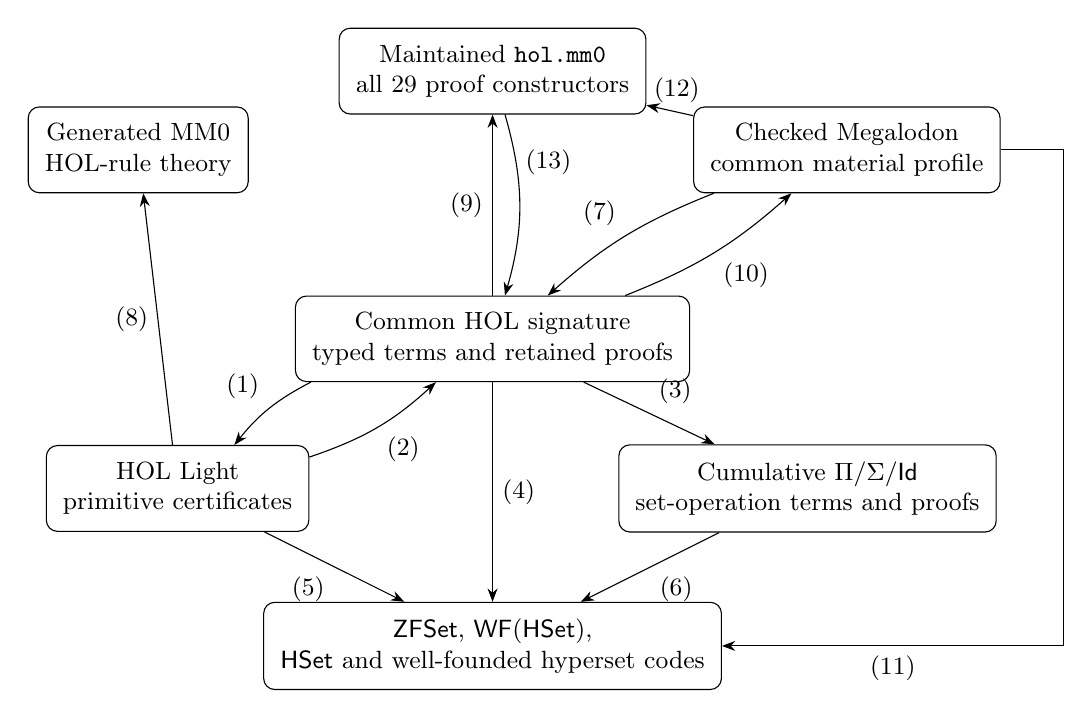
\begin{tikzpicture}[>=Stealth, every node/.style={align=center,font=\small},
  box/.style={draw,rounded corners,inner sep=6pt}]
\node[box] (hol) at (0,2.6) {Common HOL signature\\typed terms and retained proofs};
\node[box] (mega) at (4.5,5.0) {Checked Megalodon\\common material profile};
\node[box] (mm0) at (-4.5,5.0) {Generated MM0\\HOL-rule theory};
\node[box] (mm0native) at (0,6.0) {Maintained \code{hol.mm0}\\all 29 proof constructors};
\node[box] (kernel) at (-4,0.7) {HOL Light\\primitive certificates};
\node[box] (dtt) at (4,0.7) {Cumulative $\Pi/\Sigma/\mathsf{Id}$\\set-operation terms and proofs};
\node[box] (models) at (0,-1.3) {$\mathsf{ZFSet}$, $\mathsf{WF}(\mathsf{HSet})$,\\
  $\mathsf{HSet}$ and well-founded hyperset codes};
\draw[->] (hol) to[bend right=12] node[above left]{(1)} (kernel);
\draw[->] (kernel) to[bend right=12] node[below right]{(2)} (hol);
\draw[->] (hol) -- node[above right]{(3)} (dtt);
\draw[->] (hol) -- node[right]{(4)} (models);
\draw[->] (kernel) -- node[below left]{(5)} (models);
\draw[->] (dtt) -- node[below right]{(6)} (models);
\draw[->] (mega) to[bend right=10] node[above left]{(7)} (hol);
\draw[->] (kernel) -- node[left]{(8)} (mm0);
\draw[->] (hol) -- node[left]{(9)} (mm0native);
\draw[->] (hol) to[bend right=10] node[below right]{(10)} (mega);
\draw[->] (mega.east) -- ++(0.8,0) |- node[pos=.75,below]{(11)} (models.east);
\draw[->] (mega) -- node[pos=.35,above]{(12)} (mm0native);
\draw[->] (mm0native) to[bend left=16] node[pos=.25,right]{(13)} (hol);
\end{tikzpicture}
\end{center}

These are four alternative interpretations of the common signature. The
value comparisons pair $\mathsf{ZFSet}$ with well-founded hypersets, and full
hypersets with their valid codes; they do not identify well-founded sets with
all hypersets. The arrows have the following checked meanings.
\begin{enumerate}[leftmargin=*]
\item \leanname{SetOperationInterpretation.compile_accepted} and
  \leanname{compile_sequent} instantiate the complete proof compiler after a
  typed signature map. \leanname{proof_nodeCount} preserves the retained
  source proof's node count during this map; it is not a bound on the later
  primitive graph expansion.
\item \leanname{RetainedSemanticReadback.accepted_source} recovers the source
  judgment from any accepted exact closed sequent in the admitted image.
  The image excludes an uninterpreted use of the primitive equality symbol.
  Readback is proposition-valued derivability, not reconstruction of the
  original proof identity.
\item \leanname{SetOperationMaterialSemantics.native_substitution} relates
  actual term compilation at \leanname{SetOperationSignature.signature} to
  simultaneous substitution. The proof component is
  \leanname{SetOperationProofCompilation.compile_typed}, with actual native
  substitution coherence in \leanname{compile_substitute}. Its extended
  declaration profile adds precisely two opaque extensionality proof constants;
  all 29 source constructors then compile at that same profile.
\item \leanname{ZFSetSimpleTypeInterpretation.decode_interpret} compares a
  structural material graph evaluator with the independent full-domain HOL
  model. \leanname{interpret_substitution} proves its contextual coherence.
  The set and hyperset instances share this evaluator, including functional
  graphs, lambda application, equality and higher-order quantifiers.
\item \leanname{SetOperationReplay.accepted_sets},
  \leanname{accepted_wellFounded}, \leanname{accepted_hypersets} and
  \leanname{accepted_codes} validate the same checked sequent in the four
  interpretations, conditional on its listed assumptions. The further
  \leanname{accepted_hyperset_graph} theorem reaches the actual graph evaluator.
\item \leanname{SetOperationMaterialSemantics.wellFounded_graph_square} and
  \leanname{coded_graph_square} compare actual denoted values after term
  compilation. The proof component is
  \leanname{SetOperationProofCompilerSemantics.compile_proves}, instantiated
  in all four material models by \leanname{SetOperationMaterialProofSemantics}.
  It realizes the actual compiled proof at the original conclusion.
  These results do not assert soundness of arbitrary ambient DTT conversions
  or reflection of every host inhabitant.
\item \leanname{Megalodon.SetOperationProofReconstruction.checkedSource}
  reconstructs an ordinary source proof from every accepted program in the
  admitted monomorphic common profile. It returns the exact authored conclusion
  and ordered local assumptions. The six declarations are opaque; the finite
  known-fact list contains the actual functional and propositional extensionality
  instances. \leanname{ExtensionalityAxiomProofs.functionalNative} and
  \leanname{propositionalNative} construct source proofs of their exact normalized
  native readings. \leanname{withoutGlobalFacts} substitutes these proofs instead
  of appending imported facts to the source theory.
  \leanname{RelationEqualityComparison.equation} constructs the comparison of
  primitive equality with the actual binary-relation definition, using an
  explicit typed equality test and beta proofs in the reverse direction.
  \leanname{HOLTermEncodingProofs.equation} then compares every term constructor
  with its complete equality/connective encoding. Canonical hypothesis
  normalization has its own retained equation. The signature retraction preserves
  variables, open contexts, types and each named operation, including union and
  powerset despite their equal simple type.

  \leanname{accepted_profile_iff_source} equates source derivability with the
  existence of an accepted program in one of these finite explicit profiles.
  The forward compiler computes the required instances from its source proof;
  the converse consumes the checked program and constructs a source proof.
  This is an equivalence of provability, not a bijection of proofs or recovery
  of the original presentation. \leanname{accepted_meaning} consequently applies
  to any extensional Henkin model at admissible valuations, without requiring
  full function domains. The separate literal function-value comparisons retain
  their original full-domain hypotheses. Four source-reflection controls exclude
  foundation, its negation, self-membership and its negation from the six common
  operation laws. Prefix polymorphism and other declaration/definition policies
  are separate interfaces; the existing
  \leanname{CheckedProofReconstruction.checkedSourceDefined} retains explicit
  defining premises for checked bodies rather than silently identifying them
  with the opaque profile.
\item \leanname{HOLLight.RetainedMM0Compilation.compile_accepted}
  produces actual saved-proof witnesses for the generated first-order
  HOL-rule theory. \leanname{accepted_sequent_iff} gives its source-derivation
  converse. This target is distinct from the maintained \code{hol.mm0}
  presentation and its native qualification.
\item \leanname{MM0.HOLKernelProofCompilation.compile} is a total
  constructive compiler for all 29 retained source constructors into the
  maintained \code{hol.mm0} presentation. \leanname{compileFromInitial}
  allocates the complete proof after a well-formed initial native context.
  Inputs supply native sorting and checked typing for source variables and
  constants in a formation antecedent. They do not supply any compound source
  proof's translated conclusion. The exact logical antecedent retains the
  translated source assumptions in their original order, including duplicates.
  \leanname{compile_accepted} proves acceptance by the existing native proof
  checker; \leanname{compile_refuses_changed_conclusion} rejects every different
  claimed statement for that same witness.

  \leanname{HOL.ProofSyntax.binderBudget} inspects interfaces, retained term
  parameters and substitution images throughout the proof.
  \leanname{BindingDepthControls.specialization} has an arbitrarily deep
  ignored argument while its coarse proof observation and node count stay
  fixed. The node count alone therefore cannot supply this binder budget.
  \leanname{HOLKernelProofAllocation.forProof} allocates a canonical source
  bank and a working and temporary bank at each preorder proof node. The
  working root becomes a binding child's variable, and its tail becomes the
  child's canonical bank. \leanname{HOLKernelProofEnvironment.Environment.fromInitial},
  \leanname{bind} and \leanname{assume} construct the variable typings,
  formation/logical projection and ordered assumption proofs at these contexts.
  This is a sufficient finite syntactic allocation, not a native running-time
  estimate or a bound on expanded certificate size.

  Formation and logical contexts remain distinct. A canonical binder name
  inside a retained quantified assumption cannot be reused as a fresh native
  eigenvariable. Checked alpha equations are built in the formation context
  and promoted through the actual logical projection. The all-constructor
  \leanname{HOLKernelAlpha.rebind} and \leanname{HOLKernelSubstitution.compile}
  constructions provide source readback and simultaneous substitution;
  their compared raw terms need not be equal. \leanname{HOLKernelSourceBinding}
  closes GEN, abstraction congruence and CHOOSE, including the source-weakened
  child conclusion. \leanname{HOLKernelProofInstantiation} derives the actual
  SPEC, EXISTS and beta premises from the allocated environments.
  \leanname{HOLKernelExtensionality.functionExtensionality} constructs the
  needed specialization equation by application and equality congruence, then
  composes abstraction congruence with two maintained eta equations. It adds
  no new extensionality axiom. \leanname{HOLKernelProofExtensionality} restores
  the original source function and binder encodings.

  The exact maintained headers and stored logical definition bodies are read
  from the decoded theorem inventory. In particular, crossing between the
  native \code{bi} abbreviation and typed Boolean equality requires the
  checked stored body. Complete native occurrence independence and distinct
  bound images remain explicit; they impose no inequality on interpreted
  sets or hypersets. Existing variable-collapse, occupied-name, changed-body,
  swapped-premise and dependent-CHOOSE-result controls remain in force.

  The new native panel compiles the actual recursive output for one proof
  rooted at every constructor and five retained-assumption controls. All 34
  artifacts pass 220 checks: strict MM1 compilation, independent upstream C
  verification, pinned CeTTa verification, altered conclusions, removed ordered
  assumptions where present, and axiom-dependency checks. Eta remains an explicit
  dependency of the eta and functional-extensionality receipts. The Lean
  reference checker accepts all 34 and rejects 42 altered conclusions or
  assumption contexts. The untrusted serializer is checked per artifact;
  general serialization refinement and linked-C refinement remain separate.

  \leanname{HOLKernelSetOperationInterpretation.compile_accepted} specializes
  the complete compiler to the six material operations. One regular type
  parameter and six distinct regular object parameters carry their explicit
  typing antecedent. The mathematical operation laws remain the source proof's
  ordered assumptions; no set-theoretic axioms are added to maintained HOL.
  Union and powerset retain different parameter names despite their equal types.
  Four actual deductions---self-membership in powerset, cyclic union, a cyclic
  witness, and its relative equivalence to self-membership---pass 32 further
  native checks, including altered conclusions and removed premises.

  This panel exposes a concrete native-format boundary. The pinned MMB format
  supports at most 55 simultaneous bound parameters. The generic Lean allocation
  declares many unused positions; the four receipts use 22--38 bound names.
  The untrusted exporter removes unused bound declarations and records the
  resulting parameter map. Shared MM1 subproofs expand to the original printed
  proof exactly. Their tree text totals 240,787,661 bytes, the shared MM1 sources
  7,625,940 bytes, and the four verified MMB artifacts 619,600 bytes.
  These are measurements of these receipts, not an asymptotic cost theorem or
  unrestricted native-format adequacy. Existing derived native lemmas use eta
  in all four receipts; this records their actual dependencies, not necessity
  of eta for the four mathematical conclusions.

  Forward interpretation does not imply reflection.
  \leanname{HOLKernelEncodingReflection.source_not_derivable} uses a full-domain
  model to refute equality of two source Boolean constants. The typed native
  representation maps both to truth, where
  \leanname{acceptedCollapsedSource_checks} constructs an accepted reflexivity
  receipt at that encoded statement. Source reflection therefore needs an
  appropriate representation and admitted certificate image; it does not
  follow from sorting and forward compilation.
  \leanname{Kernel.ProofWitness.restricted_check_iff} isolates the local
  theorem-policy condition on the actual submitted witness. With term and
  definition tables fixed, acceptance under a restricted theorem table is
  equivalent to original acceptance and permission for every entry in
  \leanname{theoremReferences}. This ordered list includes all child proofs
  and repeated applications. \leanname{check_iff_of_theorem_agreement}
  preserves the exact judgment when unused theorem entries change, while
  \leanname{disallowed_reference_refused} excludes a denied used entry.
  Local hypotheses are retained separately. This is a dependency theorem,
  not reconstruction of a source HOL proof or a transitive axiom audit of
  imported derived lemmas. The maintained-MM0 common-profile
  readback requires the further inference interpretation below; no bijection
  of proof identities is established. These results
  qualify this interpretation of the common calculus, not every Prime profile.
\item \leanname{Megalodon.LogicalProofCompilation.compile_isSome} gives
  exact coverage of the 17 connective and quantifier proof constructors.
  \leanname{RelationEqualityProofs} separately proves actual native inference
  equations for eight equality combinators, including transitivity,
  application congruences and propositional equality elimination. These are
  proof terms, without imported known facts.
  \leanname{ProofCompilation.compile} extends the executable producer to
  all 29 retained constructors, taking explicit programs for functional and
  propositional extensionality. \leanname{logical_agreement} proves that its
  logical fragment is exactly the earlier program, independent of those
  parameters. The solid forward arrow is now supplied by
  \leanname{HOLProofCompilationCorrectness.inferred}: all 29 constructors
  infer their exact encoded conclusion under ordered canonical hypotheses,
  provided the type images are formed, term declarations are opaque, and
  each used extensionality name denotes its exact schema.
  \leanname{SetOperationCompilerAcceptance.accepted_required} instantiates
  these policies on the six-operation signature, computing its finite
  extensionality declarations from the supplied proof and constructing a
  sufficient native budget. This does not assert acceptance for arbitrary
  recursively defined or prefix-polymorphic profiles.
\item \leanname{Megalodon.SetOperationSemantics.accepted_material} proves
  soundness of the actual monomorphic Mathdata proof checker in the supplied
  full-domain material model, conditional on the source hypotheses.
  \leanname{denote_term} compares actual open-term values, and
  \leanname{sourceValuation_extend} retains context extension. The independently
  checked declaration readback distinguishes union from powerset despite their
  identical simple types. \leanname{setInduction_refused} and
  \leanname{selfMember_refused} use the hyperset and well-founded countermodels
  to exclude both conclusions from the six shared operation laws, for every
  supported proof and every checking budget.
  \leanname{SetOperationExtensionality} adds a finite list of explicitly
  declared functional-extensionality instances and propositional extensionality.
  \leanname{knownValidity} proves the meanings of those facts from the model,
  and \leanname{accepted_material} then applies actual checker soundness.
  The four positive/negative membership-induction and self-membership refusals
  remain valid with these guest axioms present.
\item \leanname{Megalodon.MM0ProofTransport.compile_accepted} composes the
  common-profile reconstruction with the independently proved maintained-MM0
  compiler. Its components use the same closed source conclusion and ordered
  assumptions. The actual target witness has the constructed material parameter
  context and complete finite allocation. This statement does not identify the
  two native proof representations or remove the separate MMB parameter/encoding
  qualification boundary.
\item \leanname{HOLKernelSetOperationReadback.readSequent_statement} reads
  the exact authored conclusion and ordered assumptions from a native common-profile
  statement. \leanname{readSequentIn_encode} covers a supplied open typed context
  and formation prefix. The shared \leanname{HOLKernelTermReadback.readTerm_encode}
  covers all 13 HOL term constructors, with explicit dictionary and name-bank
  conditions; \leanname{readType_sound} reconstructs the actual type code.
  The canonical image checks exact re-encoding after independent typed parsing.
  \leanname{statement_injective} yields refusal of a changed conclusion or
  contracted ordered assumptions for the same accepted native witness.
  This is statement reflection, not source derivation reflection. The control
  \leanname{statement_readback_is_not_derivability} faithfully reads the false
  sequent while the actual material model rules out its source derivation.

  The partial decoder \leanname{HOLKernelProofReadback.readProof}
  interprets actual checked inference trees, constructing ordinary
  retained source proofs by ordered hypothesis substitution. Its local
  interpretation covers the 21 logical/equality schemas and five structural
  schemas; actual theorem headers and native substitutions are checked.
  Boolean equivalence uses its stored definition body.
  \leanname{HOLKernelBindingInterpretation.bindingProof} reads recursive
  premises in extended intrinsic frames for GEN, SPEC, EXISTS, CHOOSE,
  abstraction congruence and substitution. Beta, eta and abstraction renaming
  construct their explicit source proofs. The native theorem headers and
  variable-independence checks remain in force.
  \leanname{HOLKernelLogicalFunctionReadback} reads the seven curried logical
  functions under their checked definitions. Native conversion is admitted
  when the source readings agree or an explicit beta recipe connects them.
  \leanname{ConversionNormalizationRecipes.betaEquality?_isSome_iff} proves
  that the existing typed normal-order evaluator supplies such a checked
  recipe exactly for beta-joinable source terms.
  \leanname{HOLKernelSetOperationProofReadback.readSourceProof} then constructs
  the explicit antecedent and restores the exact ordered source assumptions.
  The proof may choose a different equal assumption occurrence; no proof
  identity or occurrence-use correspondence is claimed.
  Intrinsic typing is reconstructed before its discharged logical reading
  becomes truth; distinct formation claims remain distinct syntax.
  Lexical binder shadowing is allowed by the general parser; eigenvariable
  freshness and the canonical name-bank condition remain distinct obligations.
  All 29 source-constructor execution controls now reconstruct proofs.
  The independent grammar \leanname{HOLKernelProofReadback.AdmittedProof}
  describes licensed local operands, ordered recursive premises, fresh binding
  frames and beta-joinable conversion without carrying a source proof.
  \leanname{readProof_of_admitted} proves total constructive reconstruction
  across arbitrary admitted nesting and context changes.
  \leanname{AdmittedProof.weakenFuel} preserves admission when its recursion
  budget grows. \leanname{readSourceProof_of_admitted} restores the exact
  ordered source sequent. Universal coverage of every compiled proof by this
  admission grammar remains open; arrow (13) concerns this admitted class,
  not every accepted native proof. The theorem
  \leanname{compilation_and_admitted_reflection} states forward compilation
  and admitted reflection with distinct certificate conditions, not an
  equivalence of one acceptance condition with source provability.
  \leanname{SetOperationMM0ReadbackSemantics.program_typed} composes the
  reconstructed source proof with the cumulative proof compiler.
  \leanname{program_substitute} retains native substitution, while
  \leanname{sets_program_readout}, \leanname{hypersets_program_readout},
  \leanname{wellFounded_program_proves} and \leanname{codes_program_proves}
  interpret that same program in the four material models.
  The totalized \leanname{AdmittedSourceProof.readback} computes its result
  with the same executable reader; \leanname{readback_read} and
  \leanname{readback_sequent} retain that computation and its submitted sequent.
  \leanname{SetOperationMM0ReadbackSemantics.admittedProgram_typed},
  \leanname{admittedProgram_substitute} and \leanname{admittedProgram_proves}
  apply directly to this admitted-certificate input. Their set, hyperset,
  well-founded and coded instances concern the actual computed dependent
  proof program, under the same explicit hypothesis meanings.
  The shared \leanname{HOLKernelStructuralReadback} constructions prove
  admission of identity, composition, pairing, projections and weakening;
  \leanname{hypothesis_admitted} and \leanname{formationProjection_admitted}
  cover arbitrary ordered entry lists. For all 21 logical/equality schemas,
  \leanname{HOLKernelInferenceReadback.read_nativeInstance} compares the actual
  instantiated native premises and conclusion with the typed source operands.
  \leanname{application_admitted} then constructs an admitted parent from its
  admitted children and checked native instance. The shared kernel inversion
  is \leanname{ProofWitness.Checks.instantiates}.
  \leanname{compile_topI_admitted} and \leanname{compile_hyp_admitted} establish
  the initial cases for the actual complete compiler over arbitrary ordered
  source assumptions.
  The environment reading now proves actual assignment and context coherence,
  admission of compiled typing premises, and preservation of admitted ordered
  hypotheses under logical assumption extension
  (\leanname{HOLKernelEnvironmentReadback.Reading},
  \leanname{initial_assumptions_admitted},
  \leanname{Reading.assume_assumptions_admitted}).
  Fresh bound-variable extension preserves the syntax reading
  (\leanname{Reading.bind}). The common name-frame transport covers terms,
  mixed judgments and every local structural, inference and binding schema.
  Its whole-tree law \leanname{AdmittedProof.rename_of_prefix} retains the
  native witness and theorem authority when that witness checks in a context
  prefix on which the new frame preserves lookup.
  \leanname{AdmittedProof.logical_weaken_of_prefix} supplies fresh-frame
  weakening for the maintained logical reader. Bounds on native substitution,
  theorem instances and checked conclusions justify this scope condition;
  a name-capture control separates arbitrary frame extension.
  The kernel law \leanname{ProofWitness.proof_in_prefix_iff} characterizes
  prefix checking exactly by acceptance in the extended context and bounds on
  every stored native variable, including child proofs and definition dummy
  images. \leanname{AdmittedProof.rename_of_varsBelow} consumes this condition.
  \leanname{initial_assumptions_varsBelow} bounds the actual initial hypothesis
  receipts by the seven parameters and source binder bank;
  \leanname{initial_assumptions_weaken_admitted} transports their admitted
  readback to a fresh frame. Logical assumption extension preserves the bound
  (\leanname{Environment.assume_assumptions_varsBelow}).
  \leanname{HOLKernelTermTyping.compileWithAssignment_varsBelow} and
  \leanname{HOLKernelTermCongruence.congruence_varsBelow} preserve the bound
  for all 13 source term constructors, including abstraction and quantifiers,
  under bounds on the encoded inputs and retained proof families. The common
  congruence owner covers the stored-definition conversion receipts.
  \leanname{HOLKernelAlpha.alphaDisjoint_varsBelow} bounds the two-bank
  alpha-renaming receipt; \leanname{rebind_varsBelow} includes the intermediate
  fresh bank for overlapping windows. Promoted rebinding and hypothesis
  transport preserve the bound. The retained environment invariant
  \leanname{Environment.ProofsVarsBelow} covers the projection, both typing
  families and ordered hypothesis receipts. Its initialization and logical
  extension laws are proved, while \leanname{bind_proofsVarsBelow} advances
  the bound to the next working-bank entry. The reader consumes it through
  \leanname{Reading.weaken_assumptions_admitted}. The actual formation
  projection is admitted through logical and bound-variable extension
  (\leanname{Reading.assume_projection_admitted},
  \leanname{Reading.bind_projection_admitted}); typing receipt admission
  follows from the reconstructed encoded term.
  \leanname{HOLKernelInferenceReadback.read_instance_of_operands} establishes
  exact ordered-premise and conclusion reading for all 21 nonbinding schemas
  over arbitrary successfully decoded native operands. Canonical native
  spellings are not required. \leanname{admittedApplicationOfOperands}
  combines these readings with the actual theorem header and substitution;
  the canonical constructors reuse it.
  \leanname{HOLKernelCongruenceReadback} now admits the actual reflexivity,
  transitivity, application and curried-application receipts. Its conversion
  law retains native witnesses and requires explicit source beta reductions.
  The seven logical function values have exact readback and beta-reduction
  laws; all seven generated logical congruence constructors consequently
  preserve admission, including stored-definition conversions and quantified
  congruence. The fresh-name law \leanname{readTermWith_encode_fresh} requires
  only that the used binder window avoid the distinct free names and the
  parameter prefix. The canonical ordered-bank theorem specializes it;
  controls separate a valid higher free name from actual variable capture.
  The stronger \leanname{readTermWith_encode_renamed} requires correct lookup
  of the source positions and permits shadowing unused target-frame names;
  the earlier finite-window law now specializes this structural proof.
  \leanname{readTermWith_encodeSubstitution} reads actual encoded substitution
  images, and \leanname{readTermWith_encodeSubstitution_weaken} proves their
  weakening under an outer binder even when an image reuses that binder's
  name internally. A positive control retains an older free variable across
  this shadowing; the capture control remains separate. These syntax laws do
  not yet establish admission of the recursive substitution proof producer.
  \leanname{HOLKernelAlphaReadback.alphaDisjoint_admitted} now covers the actual
  two-window receipt for every term constructor; \leanname{rebind_admitted}
  composes the three-window construction. Both permit an explicit source
  renaming into the reader's context. Their name-freshness hypotheses now
  protect only the source variable image, permitting an internal binder to
  shadow an unrelated target variable. Native occurrence independence, bank
  disjointness and the theorem policy remain explicit. The control
  \leanname{shadowing_fresh_for_source_not_target} separates these two
  freshness conditions. More generally,
  \leanname{readTermWith_rename_of_present} preserves successful readings
  under a name-frame map that keeps resolved variables and does not
  shadow constants. \leanname{logical_reader_weaken_of_read} adds a fresh
  variable without bounding the expression's internal binders. Failure need
  not be preserved: a previously unresolved name may acquire a binding.
  A second control shows why freshness from the variable frame alone cannot
  protect a constant dictionary entry.
  \leanname{readTermWith_encodeWithAssignment} extends pointwise compound-image
  readings through all thirteen term constructors as intrinsic simultaneous
  substitution. \leanname{readTermWith_substitution_encodings} consequently
  gives identical readings for literal insertion and encoding the
  source-substituted term, under the producer's joint finite binder budget.
  A nested-binder control retains an older free variable while proving that
  the two raw preterms differ.
  \leanname{HOLKernelSubstitutionReadback.compile_admitted} now derives
  admission of the actual recursive comparison receipt through all thirteen
  constructors. Its shared binder case joins image rebinding, structural
  weakening, pointwise congruence and the recursive lifted comparison; the
  native witness survives the assignment-lift cast.
  \leanname{HOLKernelSubstitutionReadback.instanceEquation_admitted} composes
  the actual single-variable comparison under its argument-equality assumption.
  Contextual reflexivity and transitivity supply the pointwise receipts.
  \leanname{HOLKernelSourceInstantiationReadback.deriveInstance_equation_admitted}
  reconstructs the derived equation in its fresh binder frame;
  \leanname{beta_admitted} then admits the source-derived native beta
  application with the exact renamed redex and substituted result.
  Source universal elimination and existential introduction preserve admission
  through their actual input proof and stored Boolean-equivalence conversion.
  \leanname{canonicalBeta_admitted} follows argument rebinding, function
  congruence, native beta and result rebinding back to the original encoding.
  The shared \leanname{HOLKernelStructuralReadback.promote_admitted} and
  \leanname{promoteUnder_admitted} derive admission for the existing
  projection-based context promotions, including an extra retained assumption.
  \leanname{deriveCanonicalInstance_admitted} reconstructs both receipts of
  the same prepared package at their respective source frames. Native SPEC
  and EXISTS now share \leanname{HOLKernelQuantifierReadback}, and the source
  adapters reuse that owner. Canonical universal elimination and existential
  introduction compose the actual prepared package, context promotion and
  definition conversion; the projection's native scope bound protects its
  movement into the new binder frame. \leanname{HOLKernelProofInstantiationReadback}
  specializes beta, SPEC and EXISTS to the actual allocated environment, with
  layout-derived name freshness and dictionary separation, retained premise
  admission and the environment proof-bound invariant.
  \leanname{HOLKernelExtensionalityReadback.functionExtensionality_admitted}
  follows native specialization, substitution congruence, abstraction and eta.
  Its retained pointwise premise is explicitly admitted in the fresh argument
  frame. \leanname{Reading.functionExtensionality_admitted} joins the allocated
  producer under that premise, with bounded projection transport and preserved
  whole-statement casts. Source-context rebinding needs freshness against the
  source-variable image, allowing unused target names to coincide with internal
  alpha binders; existing consumers derive this from their stronger bounds.
  The actual pointwise assignment-congruence producer now preserves
  admission through all thirteen constructors in
  \leanname{HOLKernelTermCongruenceReadback.congruence_admitted}.
  Its input receipts satisfy \leanname{AdmissionUnderRenaming}, with proved
  instances for alpha rebinding, assumption projection and weakening. Lambda
  and both quantifiers share one binding construction. The control
  \leanname{lookup_extension_can_capture_eigenvariable} explains why
  successful term-reader transport alone does not preserve arbitrary proof
  admission: a new frame variable can violate a rule's eigenvariable condition.
  Promoted rebinding, Boolean equality
  conversion/elimination and \leanname{weakenAssumption_admitted} retain the
  actual receipts through context extension and conclusion casts.
  \leanname{Reading.bind_assumptions_admitted} proves this invariant for every
  ordered hypothesis occurrence in the allocated environment.
  The actual source universal-introduction, abstraction-congruence and
  existential-elimination constructions now preserve admission through their
  native GEN, abstraction and CHOOSE steps, rebinding and equality joins.
  Existential elimination transports the retained projection to the witness
  frame under an explicit raw scope bound and preserves its conclusion cast.
  The shared \leanname{AdmittedProof.logical_weaken_of_varsBelow} supplies this
  transport in an arbitrary native context.
  \leanname{Reading.eta_admitted} follows the actual allocated eta producer
  through both rebinding receipts, its native eta application, symmetry and
  transitivity. \leanname{compile_eta_admitted} consequently admits the complete
  compiler's eta output for arbitrary closed function terms and ordered
  assumptions. Its later-window readings and rebinding admission follow from
  the existing environment and retained formation projection.
  \leanname{HOLKernelProofCompilationReadback.compile_admitted} now proves
  independent admission of the actual compiler image through all 29 source
  constructors. Its contextual reading invariant allows additional reader
  variables and derives admission of the actual environment leaves.
  Extensionality invokes the child induction in its fresh argument frame;
  arbitrary proof-tree weakening is not assumed.
  \leanname{closed_compile_admitted} specializes the initial environment, and
  \leanname{closed_compile_readback} reconstructs the original ordered sequent.
  \leanname{admitted_certificate_iff_derivable} equates source derivability
  with existence of an independently admitted certificate under the specified
  native schema and reader policies. It does not assert arbitrary-certificate
  reflection or proof-identity recovery. The complete route is
  \[
  \begin{array}{c}
    \text{retained HOL proof (all 29 constructors)}\\
    \downarrow\ \texttt{compile\_accepted}\\
    \text{actual maintained-MM0 certificate}\\
    \downarrow\ \texttt{closed\_compile\_admitted}\\
    \text{independently admitted certificate}\\
    \downarrow\ \texttt{readSourceProof\_of\_admitted}\\
    \text{computed HOL proof at the original sequent}\\
    \downarrow\ \texttt{admittedProgram\_typed},\ \texttt{admittedProgram\_substitute}\\
    \text{cumulative }\Pi/\Sigma/\mathrm{Id}\text{ proof program}\\
    \downarrow\ \texttt{compiled\_readback\_program}\\
    \text{ZFSet, WFHSet, HSet, or coded-HSet interpretation}.
  \end{array}
  \]
  The final arrow uses \leanname{admittedProgram_proves} with the chosen
  model's full-domain theorem and the meanings of the source hypotheses;
  \leanname{admitted_sets_readout}, \leanname{admitted_hypersets_readout},
  \leanname{admitted_wellFounded_proves} and \leanname{admitted_codes_proves}
  supply the four material specializations. Native schema selection, binder
  apartness and the separate membership relations remain explicit.
  The scoped programme is now qualified by 232 strict roots and consumers
  against an unchanged 15,580-source dependency cohort. All 43 executable
  reconstruction cases and 441 fresh pinned native checks pass. The foundation
  audit covers 15,412 safe kernel declarations; 132 generated runtime
  implementations are recorded separately. The selected strict targets have
  zero warnings, while the dependency build's warning inventory remains
  explicit. These checks qualify the recorded sources and native artifacts,
  without claiming a C implementation refinement theorem.
\end{enumerate}

The common source vocabulary is owned by \leanname{Logic.HOL.SetOperationSignature}.
\leanname{HOLKernelSetOperationSyntax} supplies the native parameter representation
and formation context; the inference compiler retains its separate owner.
The existing declaration names and mathematical bodies are retained.
The native reader preserves the identities of union and powerset despite their
shared simple type. It refuses inconsistent equality type annotations and
parameter capture. Distinct alpha spellings can decode to the same intrinsic
lambda; only the canonical image supplies exact spelling recovery.
The name-collapse control retains the explicit distinctness condition.
None of these representation results licenses arbitrary theorem-table entries.

The cumulative calculus also supports a constructive predicate-equality proof
reading of this same six-operation signature.
\leanname{HOLPredicateEqualitySignature.equality_typed} forms the actual
native equality lambda; \leanname{application_conversion} derives its two
beta steps without installing an equality decoder or a native identity equation.
\leanname{HOLPredicateEqualityOperations.operations} constructs six lawful
proof operations, with native substitution laws. Proposition and function
extensionality are absent from this particular algebra.
\leanname{SetOperationPredicateProofs.compile_typed} applies the existing
recursive compiler to every successful expansion, and \leanname{compile_substitute}
preserves its actual optional output under native context substitution.
\leanname{union_typed} and \leanname{power_typed} check the independently
displayed congruence programs. They retain different operation names despite
the shared simple type. A propositional-extensionality presentation is refused
while reflexivity at the same conclusion succeeds. This is a boundary of the
chosen proof operations, not a non-derivability result. \leanname{HenkinModel.functionsRespectEqv_iff_predicateEquality} derives the
exact semantic condition for agreement of unary predicate equality with intrinsic
equality on admitted values. A concrete lambda-closed monotone model separates
two admitted endpoint functionals with equal intrinsic readings by an admitted
predicate. \leanname{HOLPredicateEqualitySemantics.native_equality_value}
interprets the actual equality lambda through the original signature's lambda,
quantifier and implication clauses. Equality of its entire binary function uses
coverage of the endpoint type; its admitted-value comparison needs no full-domain
assumption. \leanname{SetOperationPredicateSemantics} supplies the well-founded
set, well-founded hyperset, full hyperset and coded-hyperset instances.
The separate \leanname{SetOperationExtensionalProfile} adds two opaque,
formed proof declarations expressing proposition and function extensionality.
Their types use the same predicate equality and the shared proof-family name;
neither changes native identity or the calculus's conversion relation.
\leanname{SetOperationExtensionalOperations.operations} constructs all eight
compiler capabilities, with totality and substitution naturality. The two
extensionality programs supply their actual arguments, including native domain
and codomain codes for function extensionality.

\leanname{SetOperationProofFamilySemantics.Denotes} independently interprets
native variables, abstraction, application and explicit family recoding, with
clauses for these two fully applied opaque proof operations. The six remaining
capabilities are realized by their actual lambda/application programs in
\leanname{SetOperationPredicateFamilySemantics}. Thus
\leanname{SetOperationProofCompilerSemantics.algebra} constructs every local
semantic obligation before applying the generic compiler theorem.
\leanname{compile_proves} realizes the original, unexpanded HOL conclusion
of the actual computed native proof. This proof-family reading uses full HOL
domains: its ordinary dependent products range over all carrier values.
No necessity claim for other possible interpretations follows from that choice.
\leanname{compile_proves_of_original_hypotheses} retains ordered authored
hypothesis meanings, and \leanname{SetOperationKernelProofSemantics.accepted_program_proves}
constructs the proof and its meaning from an accepted common-profile Megalodon
program, without a supplied source proof.

\leanname{SetOperationMaterialProofSemantics} instantiates this proof
interpretation in the four material models. The separated-singleton proof codes
are determined by the independent set and hyperset graph evaluators.
\leanname{setGraphProofCode_substitution} and its hyperset analogue preserve
source substitution; their implication laws identify the actual trace-coded
dependent product. The well-founded and coded comparison squares agree at
these proof codes. \leanname{distinct_programs_same_material_reading} gives
two distinct native proof programs with the same material proof reading.
The retained \leanname{semantic_codec_does_not_reflect_values} control
separates this chosen realization from unique native execution meaning.
The result concerns the compiled HOL fragment and fully applied opaque
operations, not arbitrary native universe terms, partial opaque applications,
identity reflection or a new C implementation of dependent proof checking.

The material exports include deductions from powerset and empty-set laws and
an explicitly cyclic union instance.
\leanname{MM0.HOLMaterialProofExport.cyclicUnionProof} derives
$q\in q\Rightarrow q\in\bigcup q$ from the union law.
\leanname{cyclicUnionEquivalenceProof} gives a retained proof that, over
that same law, the existence of $q$ with both $q\in q$ and
$q\in\bigcup q$ is equivalent to the existence of a self-member.
\leanname{cyclicUnionWitness_iff_selfMember} proves this equivalence over
arbitrary Henkin models without full-domain or choice hypotheses.
The cyclic premise is realized by the Quine hyperset; an actual well-founded
model proves \leanname{cycle_premise_cannot_be_dropped}.
\leanname{coded_cycle_instance} retains the actual encoded union of that
same value, with cyclic interpreted membership and irreflexive host membership.
These deductions explore compatible interpreted fragments without selecting
an ambient foundation for all Prime candidates.

The equality comparison also gives an exact relative-strength boundary.
\leanname{Megalodon.RelationEqualityExtensionality.functionalExtensionality_iff_functionsRespectEqv}
identifies functional extensionality for Megalodon's binary-relation equality
with extensional argument congruence on admitted Henkin values.
The set, hyperset and coded models satisfy it; the lambda-closed
monotone-Boolean model refutes it. Full function domains suffice but are not
asserted necessary. Propositional extensionality is already valid in the
chosen Henkin interface's proposition carrier. These are principles of an
interpreted fragment, not a conclusion about every proposition or identity
type of an ambient Prime candidate.
\leanname{ExtensionalityAxioms.Native.functional_normalizes} and
\leanname{propositional_normalizes} identify the actual normalized native
schemata with their typed formula interpretations.
\leanname{functional_valid} derives the former's validity from extensional
argument congruence, without full-domain or material-choice hypotheses;
\leanname{propositional_valid} uses the chosen proposition carrier.

The hyperset replacement construction uses an explicit graph presentation;
\leanname{HSet.Presentation.choice} supplies one in the classical checking
metatheory. \leanname{CodedFamilyCwf} constructs context extension and a full,
faithful decoding functor. \leanname{CodedFamilyTypeOperations} equips that
same CwF with actual dependent products and sums, their beta/eta laws and
strict substitution laws. The comparison is contextual:
\leanname{CodedFamilyTypeComparison.piFamily_comparison} and
\leanname{sigmaFamily_comparison} compare the actual type sets after
transporting the codomain through comprehension.
\leanname{lam_comparison}, \leanname{app_comparison},
\leanname{sigmaPair_comparison}, \leanname{sigmaFirst_comparison} and
\leanname{sigmaSecond_comparison} compare the constructed term operations,
with the dependent result-family transports explicit. Cyclic values are
admitted, while \leanname{empty_codomain_no_section} retains the empty-fibre
obstruction. In the coded interpretation,
\leanname{CodedHypersetInterpretation.memberships_distinct} exhibits one code
with interpreted self-membership and no host self-membership. Under the
stated closure predicate, \leanname{HypersetHOLTypeInterpretation.all_typeCodes_mem_iff}
identifies the extra carrier-code containment needed to contain every simple
HOL type code. This is a closure characterization; it is not a necessity proof
for inaccessible cardinals.
\leanname{ZFSetTarskiUniverses.inaccessible_tarski} additionally proves all
three local clauses of Tarski's Axiom A for inaccessible rank segments:
subset closure, internal bounds on powersets, and the cardinality alternative
for every subset of the universe. \leanname{exists_common_enclosure} constructs
one set satisfying both this property and the existing Grothendieck closure
predicate, under cofinal inaccessible cardinals. This is a common sufficient
model construction, not the full equivalence of the axiom packages studied
by Brown and P\k{a}k \cite{BrownPakTwoSetTheories}.
\leanname{HypersetHOLTermInterpretation.exists_tarski_envelope} places all
simple-type codes and interpreted term values in one such host universe.
Its cyclic-guest control keeps the two memberships distinct. Indeed,
\leanname{CodedHypersetInterpretation.no_membership_preserving_map_to_sets}
shows that even forward preservation into host membership is impossible on
the whole hyperset carrier: a Quine atom would become a host self-member.

The two models also separate principles of the common theory.
\leanname{HypersetHenkinInterpretation.setInduction_independent} and
\leanname{selfMember_independent} give positive interpretations on both sides
of each independence claim. At the checking boundary,
\leanname{SetOperationReplay.foundation_refused} and
\leanname{negatedInduction_refused} rule out both induction and its negation
from just the six common laws under the eta-only policy. Negated induction
is not being identified with a complete anti-foundation axiom package.

The distinction between a classical guest and its host is also modeled
contextually. \leanname{ConstantPresheafInterpretation} sends complete typed
valuations and term denotations to constant presheaves, preserving context
extension and substitution. Under full source domains,
\leanname{universal_reading} and \leanname{existential_reading} compare HOL
quantifiers with the ambient all-future operations. All 29 proof constructors
are sound in that same context. \leanname{ConstantPresheafControls} instantiates
the actual hyperset model over the existing advancing-world category.
\leanname{excludedMiddle_in_fragment} holds for its closed proposition image,
while \leanname{laterTruth_not_in_image} exhibits a stable predicate outside
that image and \leanname{ambient_doubleNegation_fails} refutes ambient Boolean
logic. \leanname{guestChoice} coexists with
\leanname{emptyObject_has_no_section}; choice is not extended to the empty
ambient object.
\leanname{excludedMiddle_of_predicate_coverage} states the sufficient condition
for globalizing this classicality: every ambient predicate of the chosen
context must be the actual interpretation of a source formula. Equality of
predicates supplies preservation and reflection of their truth at every point.
\leanname{oneWorld_predicate_coverage} and \leanname{oneWorld_excludedMiddle}
give a positive instance with the same hyperset guest over one world;
\leanname{closedMeaning_not_surjective} records the failure of coverage in
the advancing-world host. Coverage is a sufficient condition, not asserted to
be necessary for a host that is independently Boolean.
The construction uses classical external metatheory, while
the separating logic is internal to the specified presheaf host.

The reconstruction also separates logical equality from evaluation.
\leanname{RetainedDefinitionControls.no_definition_free_proof} gives an
independent interpretation refuting the source claim when its defining
premise is omitted. Conversely, \leanname{DefinitionErasure.proof} transforms
the same reconstructed proof to the original signature by substituting the
actual defining body and discharging the resulting reflexive equation. The
expanded claim has no defining assumptions; the opaque claim does not thereby
acquire a definition-free proof. \leanname{Cyclic.all_fuels_exhausted} exhibits a typed
self-referential definition whose equation has a reflexivity proof but whose
unfolding exhausts every finite budget. A proof of equality is therefore not
a termination certificate. The exact beta/eta normalization comparison,
including failure, remains \leanname{RetainedNormalization.normalize_erases}.
\leanname{Megalodon.HOLTermEncoding} separately translates every HOL term
constructor to Megalodon's actual binary-relation equality and impredicative
connectives. \leanname{encode_subst} and \leanname{denote_encode} preserve
substitution and full-domain meanings; \leanname{native_infers} exposes the
selected type-depth formation check. The logical proof fragment and native
equality combinators above extend this term translation.
\leanname{HOLTermConversion.encode_step} preserves beta and eta steps
through both equality expansion and connective expansion, and
\leanname{native_opaque_coherent} compares actual normalized outputs when
the inputs contain no expandable declaration. This is preservation rather
than reflection of source conversion: primitive truth and its quantified
encoding have identical target syntax but are distinct source beta/eta
normal forms (\leanname{same_encoding_does_not_reflect_conversion}).
The shared \leanname{BetaEtaSubstitution} laws retain renaming and
simultaneous substitution below binders.
The all-constructor forward Megalodon theorem below concerns its explicit
opaque profile. Prefix-polymorphic proof reconstruction, unrestricted delta
policies, and general acceptance and reflection theorems for the
maintained-\code{hol.mm0} proof exporter remain open.
For the normalization obligation,
\leanname{Logic.HOL.EtaPostponement.postponement} factors every typed
beta/eta path into beta steps followed by eta steps. Its strict interaction
law retains nonempty beta progress, giving
\leanname{BetaEtaNormalization.stronglyNormalizing} for arbitrary
interleavings, over all HOL term constructors and contexts.
\leanname{BetaEtaConfluence.confluent} establishes confluence of the combined
relation by joining the mixed local forks; distinct variables remain
nonconvertible. These results use the existing typed relations and shared
relation-theoretic accessibility constructions.
\leanname{Megalodon.NormalizationTermination.normalizeOne_steps} connects
the actual monomorphic pass, including its stability flag, to genuine
reduction progress. The executable \leanname{complete} computes a sufficient
budget for that pass; \leanname{completeNative} extends this guarantee to the
delta/beta/eta pipeline when the input contains no expandable declaration.
\leanname{HOLLightNormalizationCompletion.certificate_accepted} composes the
computed budget with the retained equality compiler: every admitted intrinsic
monomorphic input produces an accepted primitive HOL Light receipt, without a
successful-run premise. Its \leanname{certificate_sequent} gives the exact
translated equation and empty logical assumptions, under the explicit eta
axiom policy. This theorem concerns normalization receipts rather than
acceptance of arbitrary forward proof programs.
\leanname{NormalizationNormalForm.stable_normal} proves that the actual
pass's stable flag excludes every beta/eta step on its admitted grammar.
\leanname{normalize_coherent} consequently equates the actual raw outputs
of any two successful budgets on beta/eta-convertible intrinsic inputs.
\leanname{decideConversion_correct} combines computed completion and this
normal-form comparison into a decision procedure for that typed monomorphic
conversion relation.
For the common material signature,
\leanname{SetOperationExtensionality.normalizeTerm_meaning} preserves the
actual value under every open valuation in every supplied full-domain set or
hyperset model. Its typed output is fixed before the model is chosen.
The cyclic-definition control still exhausts every delta budget. General
definition unfolding and prefix type computation remain outside this
completion result. The all-constructor opaque-profile compiler uses this
normalization coherence. Existing budget-monotonicity and finite-common-bound
theorems join successful local checks.
\leanname{TypedProofApplication.term_application} uses those bounds and the
typed substituted body to construct a successful native proof application.
Its body's definition-normal support follows from the checked function and
the context support invariant; argument annotation formation and support
remain explicit. \leanname{proof_application} joins two checked programs at
the maximum of their budgets, retaining the same ordered context and exact
intermediate proposition.
\leanname{HOLProofSpecialization.allE2} and \leanname{allE3} use the shared
\leanname{Logic.HOL.instantiate_subst_lift} law to express repeated universal
specialization as one simultaneous substitution. The logical, existential,
equality and extensionality constructions now cover all 29 source rules and
are joined by the complete \leanname{HOLProofCompilationCorrectness.inferred}
induction on the supplied proof tree.
\leanname{SetOperationCompilerAcceptance.functional_declared} verifies the
actual indexed declaration lookup for each requested instance, including
repeated type pairs. \leanname{accepted_required} computes sufficient
checking budgets and the finite instance list, rather than assuming a
successful run. \leanname{SetOperationCheckedCompilation.checkingBudget}
makes this selection executable using the computable least-number operator.
Its \leanname{checkingBudget_accepted} and \leanname{checkingBudget_failure_below}
prove success and minimality for the reference checker's normalization
parameter. Certificate size, receipt grade and native runtime cost are
separate quantities. \leanname{compiled_fragment} proves that every resulting
program lies in the existing monomorphic semantic replay fragment.
\leanname{checked_material} joins acceptance of this same program to its
material interpretation. Its \leanname{canonical_formula_meaning} and
\leanname{accepted_canonical_material} preserve the interpreted propositions
of the ordered canonical hypotheses in every supplied full-domain model.
This normalization of hypotheses is part of the admitted representation;
\leanname{SetOperationCompilerControls.authored_hypothesis_refused} shows
that supplying an authored redex as an unnormalized hypothesis can fail the
reference check. The canonical representation accepts, and duplicate
hypotheses retain their distinct indices.
\leanname{HOLProofInference.refuses_other_normal_form} refuses every changed
canonical conclusion at every budget. Source beta/eta conversion reflection
and recovery of the original proof identity are not consequences of these
forward theorems.
\leanname{ProofCompilationDefinitionBoundary.compiled_reflexivity_requires_delta}
derives a necessary condition from the actual Boolean checker: acceptance of
compiled source reflexivity forces its encoded argument's delta phase to
finish at the same budget.
\leanname{compiled_cyclic_rejected}
shows why typed declarations alone cannot replace the profile's unfolding
conditions: the source has a reflexivity proof for a recursively defined
constant, while its actual compiled program is rejected at every budget.
\leanname{opaque_argument_accepted} accepts the corresponding program when
the same name is declared opaque. This boundary concerns native definition
unfolding, independently of the cyclic membership of material hypersets.
Conversely, \leanname{SelectedTheoryProfile.opaque_profile_rejects} retains
the control where hiding a needed definition invalidates a proof. A
transport must therefore expose its definition and equation policy; opacity
alone is not a general preservation theorem.

MM0's bound names require an additional contextual distinction.
\leanname{MM0.Kernel.Substitution.two_bound_admissible_iff} characterizes the
actual two-bound substitution guard by inequality of target names.
\leanname{MM0.HOLContextRenaming.independent_names_equal_sets} and its
hyperset counterpart give admissible valuations assigning the same value to
distinct names. At the concrete cumulative signature,
\leanname{MM0BoundContexts.native_identification}, \leanname{set_identification}
and \leanname{hyperset_identification} prove that ordinary object-variable
identification commutes with term translation and material interpretation.
Nevertheless, \leanname{typing_does_not_admit_bound_collapse} shows that this
DTT typing provides no authority to bypass the MM0 guard. A reflecting
comparison must retain name independence separately from semantic values.

For operational meaning, \leanname{FiniteBranchingHypersetSemantics.readout_observe}
factors small labelled coalgebra decoration through final observation.
Injective label encoding gives \leanname{readout_eq_iff_bisimilar}; the GSOS
instance \leanname{initial_final_readout} compares the compatible initial/final
semantics. Actual CCS and HOL primitive-replay instances retain the size and
label hypotheses. \leanname{HypersetReplay.origin_not_determined_by_meaning}
separates future replay behaviour from past receipt origin, whereas
\leanname{repeated_cache_entry_changes_meaning} shows why cache multiplicity
can change a future indexed lookup. Neither a behavioural quotient nor a
conversion judgment by itself specifies which history a runtime stores.

The higher-order extension has separate obligations. Goncharov et al.
\cite{GoncharovHigherOrderDenotation} use a mixed-variance behaviour bifunctor
$B:\mathcal C^{\mathrm{op}}\times\mathcal C\to\mathcal C$ and a locally final
coalgebra $Z\to B(Z,Z)$, final for $B(Z,-)$. Their extension theorem requires
relative flatness of the higher-order GSOS law; general recursion can violate
that condition. Adequacy concerns the selected behavioural equivalence.
Applying this route here requires a binding-aware signature and substitution,
the corresponding higher-order law, a suitable local-finality construction,
and a material comparison respecting those observations and universe bounds.
None follows from finite-branching hyperset decoration alone. This extension
remains outside the completed first-order comparison; increasing the universe
by itself does not discharge its mixed-variance obligations.

Pinned native qualification currently covers all 29 HOL proof-constructor
fixtures with exact canonical conclusions and axiom-dependency checks,
material-signature deductions, and the Megalodon-to-HOL normalization examples.
The powerset and definition-conversion examples are checked through both
Megalodon's native authority and HOL Light, with exact authored conclusions;
changed declarations and omitted defining premises are rejected.
The qualification record separates positive checks, forged conclusions and
changed policies. It is executable evidence for the recorded binary and
inputs, not a formal refinement proof for the C implementation or a
linear-time bound for arbitrary certificate checking.
The resumed transport qualification adds 41 maintained-MM0 exports, checked
against an independently printed specification by both the upstream verifier
and the pinned native runtime. The same four material deductions are also
checked through HOL Light. Megalodon's additional panel checks 26 equality
programs, 18 logical-rule and assumption-occurrence examples, five material
deductions and two final-conversion controls, each with a refused altered
conclusion. Instance qualification and universally proved checker soundness
remain separate claims.
The full Megalodon producer has a further 123 checks over 36 retained-rule,
context and binder cases and five material deductions. The two added cases
retain reducible hypotheses and duplicate occurrences through canonical
context normalization. Each checks its exact
authored conclusion, refuses an altered conclusion, and tests removal of the
declared extensionality facts. Four compiled programs use those facts and are
refused under the changed profile. This is a dependency of these programs;
it does not prove their particular conclusions require extensionality.


The constructive common-profile reconstruction panel runs 42 programs, including
all 29 retained constructors, material deductions and an open-context duplicate
hypothesis. All 126 exact-conclusion, altered-conclusion and changed-profile
checks pass through the pinned native checker. The Lean producer also executes
the source reconstruction on each accepted program. A separate raw truth program
is reconstructed and passed to the maintained-MM0 compiler without an input source
proof. Its exported artifact passes strict upstream compilation, upstream C and
pinned native exact-statement verification, both forged-conclusion refusals and
an axiom-dependency check (six checks). Removing unused bound declarations leaves
five used bound names; the proof text is unchanged. These are per-artifact
qualifications, not a proof of a general native serializer or arbitrary MM0
source reflection.

\section{Universe services for reflective reasoning}

\subsection{A type-theoretic analogue of universe selection}

A literal Grothendieck universe is an extensional set-theoretic object.  It is
therefore a category mistake to ask an intensional dependent type theory to
contain that very object without first supplying an internal set interpretation.
The useful design question is instead whether dependent type theory can recover
the same \emph{one-motion ergonomics}: start with the family currently under
discussion, move to a universe containing it, and continue using the ordinary
closed constructions there.

The natural generator in dependent type theory is not a single untyped set but a
dependent family
\[
  A:\mathcal U_i,
  \qquad B:A\to\mathcal U_i.
\]
A \emph{family-enclosing Tarski universe} over $(A,B)$ consists of codes $U$,
a decoder $T:U\to\mathcal U_i$, codes for $A$ and every $B(a)$, and code
constructors closed under a declared collection of type formers.  The useful
profile here contains $0$, $1$, $\mathbb N$, binary sums, dependent products,
dependent sums, identity types, and W-types.  Decoding laws are equivalences,
not definitional equalities; this avoids silently installing equality reflection
or a particular conversion algorithm.

A \emph{family-enclosing universe operator} is then a uniform operation
\[
  \mathsf{Enclose}(A,B)=(U_{A,B},T_{A,B}).                \tag{4}
\]
Palmgren introduced precisely this universe-above-a-family idea and distinguished
it from a superuniverse which is itself closed under the universe operator
\cite{PalmgrenUniverses}.  Equation (4) is the clean type-theoretic counterpart
of ``choose a Grothendieck universe large enough for the present data.''  It is
not an assertion that types are sets, nor that there is one completed universe
of all types.

The current formal development establishes the following capability-level
result.

\begin{theorem}[Predicative family enclosure]
At every ambient type level, every dependent family has a family-enclosing
Tarski universe with the closure profile above.  Its $\Pi$- and $\Sigma$-closure
instantiate the common universe-capability interface.  A nonconstant family with
fibres $1$ and $2$ is enclosed as a positive dependent control.  The ambient
code carrier cannot code itself at the same level.
\end{theorem}

That capability-level witness uses the next metatheoretic level as its code
carrier.  A separate generated construction strengthens it.  For a family
$(A,B)$ at level $i$, define a strictly positive, type-indexed grammar
\[
  \mathsf{Gen}_{A,B}(T):\mathcal U_{i+1},
  \qquad
  U_{A,B}=\sum_{T:\mathcal U_i}\mathsf{Gen}_{A,B}(T),
  \qquad
  \mathsf{El}(T,g)=T.
\]
Its constructors retain the base and fibre generators and the complete
formation derivations for $0,1,\mathbb N,+,\Pi,\Sigma,\mathsf{Id},W$.
Dependent constructor premises range over their decoded domains; the grammar
therefore admits arbitrary nonconstant families of previously generated codes.
The code carrier consists of generated derivations, rather than the entire
ambient type universe with its identity decoder.

\begin{theorem}[Generated enclosure and material decoding]
The generated grammar encloses every generating family.  Substitution of
generators preserves its decoding and satisfies identity and composition laws.
Successor embeddings have coherent decoding comparisons for
$\Pi,\Sigma,\mathsf{Id},W$, including their application, projection and tree
operations.

For arbitrary material sets $X:\mathsf{HSet}_i$ and material families
$B:\mathsf{El}(X)\to\mathsf{HSet}_i$, the dependent core grammar generated by
their actual member types has a constructed material interpretation.  Every
derivation built using $0,1,\Pi,\Sigma,\mathsf{Id},W$ receives a graph at bound
$i+1$, an explicit inverse member decoder, and uniform term graphs.  These
constructions include arbitrary nested nonconstant families and W-types with
arbitrary dependent position carriers.  Their complete interpretation commutes
with substitution.  The core code carrier lies at type level $i+2$; its
interpreted type values form a material enclosure at graph bound $i+2$.
Raising the original material family preserves interpreted values through
proved decoder equivalences and embeds the lifted enclosure into the enclosure
generated over the raised family.
\end{theorem}

The constructions are checked in the general type-theory and hyperset library.
They require no selected Prime or Megalodon theory, no chosen representatives
of quotient classes, and no independently supplied section carrier.  The
material core theorem does not assign host-valued decoders to the broader
grammar's natural-number and binary-sum conveniences.  Graph labels that
distinguish natural numbers are a different capability from a decoder that
recovers a host natural number from an arbitrary material member.

The material interpretation uses discrete identity fibres and their dependent
eliminator.  This is a stated model profile, not a global rule imposing UIP or
equality reflection on native identity.  The separate presentation-groupoid
comparison retains automorphisms and proves dependent elimination for natural
motives; its occurrence-sensitive controls distinguish identity witnesses that
material equality forgets.  An actual functor from presentation isomorphisms
to discrete material values preserves dependent elimination for coherent
observed motives.  The material member family is nonconstant, but every loop
acts trivially after discrete descent.  The occurrence family has a nontrivial
loop action and therefore cannot descend, even through a natural equivalence
of fibres.  This is a proved obstruction to erasing identity evidence, not a
global axiom of equality reflection.

The discrete model's successor-site comparison also retains the complete
two-endpoint and identity-witness context.  Dependent J, its computation
rule, naturality and commuting substitution are checked for arbitrary
natural motives at the raised site.  Actual lifted lower material motive
dictionaries have corresponding J-value and inverse-member decoder laws.
The latter comparison concerns those translated dictionaries; it does not
assert descent of every arbitrary upper material motive.

The contextual construction retains the complete displayed family and its
material dictionaries.  Its dependent products observe every future context
and actual arrow; its inductive trees satisfy hereditary naturality across
those arrows.  Substitution of full families, and W-type comparison across
actual base-presheaf substitutions, are checked with decoder, restriction,
constructor and fold comparisons.  Equal present carrier sets cannot be
used as complete universe codes: the growing family and the unit family
have the same carrier now and different carriers along a real future arrow.
This obstruction survives universe lifting.  The full-family code quotient
instead has proved substitution equations and a natural family decoder.
A constructor-closed quotient now descends $\Pi,\Sigma,\mathsf{Id},W$
through proved constructor congruence and dependent quotient elimination.
Its decoder retains the complete family rather than only present carriers.
The equations preserve formation recipes: two codes can decode to identical
complete families and still remain distinct.  Fresh formation after a
substitution is compared through actual natural member equivalences and
material-value laws; semantic agreement does not by itself identify codes.
In particular, a noninjective context substitution can change the labels of
freshly constructed W-leaves.  Their values need not equal those of trees
transported from the original construction.

The successor construction now closes a new code grammar using previously
constructed lower codes as its cumulative seeds.  Independent upper
$\Pi,\Sigma,\mathsf{Id},W$ formation remains available, with constructed
dependent comprehension comparisons to lifted lower formation.  A
seed-sensitive trace proves that the cumulative code embedding is injective,
including for distinct codes with identical complete decodings.  Two actual
successor sites and code grammars are constructed by re-instantiating the
seed, model and arrow data; their members, natural sections, restrictions,
decoders and substitutions commute with the two successive lifts.  Fresh
upper recipes need not be cumulative seeds.  Recursive lifting of a lower
generation derivation separately rebuilds every constructor from primitive
seeds and transports dependent bodies through the constructed comprehension
equivalences.  These are actual constructions at each displayed successor
level, not iteration of an assumed enclosure operation.  They do not provide
a term-indexed sequence of variable host universe levels or internal
transfinite closure.

Bare material carriers with authored member restriction maps also receive a
constructed contextual interpretation.  Uniform membership graphs present
every lifted carrier, and an explicit inverse member equivalence builds its
decoder without selecting an original graph representative.  The site and
graph bound rise by one level.  Arbitrary bare dependent bodies over the
actual raised comprehension support generated $\Pi,\Sigma,\mathsf{Id},W$;
they need not be constant along the projection.  Complete family substitution
and inverse natural-section comparisons are checked.  Original-level
smallness of each individual fibre must still be distinguished from
original-level smallness of the entire family-parameter space.

The general authored grammar also has a constructed mixed-bound material
enclosure.  With context bound \(u\) and external parameter bound
\(\max(u,v)\), its actual generated carriers are collected at graph bound
\(\max(u+1,v+1)\).  The inverse decoder recovers a native term from an
enlarged member of a retained code, and the whole-section decoder retains
every restriction map.  Its material comprehension is naturally
isomorphic to the pullback of the constructed universal small family.
Classification, decoding and parameter substitution commute as whole
natural maps.  Further maximum-bound embeddings preserve and reflect
membership and agree with direct embeddings.  An infinite observed-family
control has equal present carriers and different future support, even
after enlargement.  These enclosures therefore retain their codes and
dictionaries; a bare present material carrier is not a decoder for the
full family or its formation recipe.

The contextual power construction retains a stable predicate on every
future context, actual arrow and argument.  Its existential direct image
and inverse image satisfy an order adjunction; an explicitly constructed
argument-family pullback satisfies the complete-future Beck--Chevalley
equation.  Singleton and union are natural in both context and argument,
with both unit laws and associativity.  For arbitrary small parameter
families $B$ and argument families $A$, natural maps
$B\to\mathcal P(A)$ correspond, with constructed inverses, to stable
predicates on the actual product $B\times A$.  This correspondence
commutes with parameter substitution.  Faithful material labels for all
future arguments supply the full member decoder.  Whole material values
are preserved when those labels are transported; independently fresh
labels preserve decoded truth through an equivalence.  Actual dependent
substitutions construct inverse future-argument comparisons and inverse
natural-section comparisons, including at the raised site.

Infinite labelled-history controls separate the full contextual power
from its present subset, even for natural classifiers with an actual
parameter family.  Two predicates can have the same empty present part
and different future material values.  A context functor that omits a
future can destroy injectivity; arbitrary context functors therefore
require their stated coverage and lifting hypotheses.  These power
constructions concern interpreted small argument objects.  A small
powerclass of arbitrary large objects, its quotient and collection
properties, and indexed finality remain distinct construction obligations.

For argument objects at an independently larger host level, a further
construction retains stable predicates with small receipt covers at every
complete future index.  The existence of a uniform receipt family is part
of the admitted predicate, not a choice of its enumeration.  Restriction
and direct image construct the new covers; identity, composition and the
natural singleton map are checked.  On originally small argument families,
the actual truth subtypes construct an inverse comparison with the full
contextual power.  The output bound includes both the context level and
the argument level, while its receipt bound stays fixed.

This larger construction has a discriminating size obstruction.  Any
surjective small cover of all hypersets would construct a small membership
graph whose decoration and range form a universal hyperset, contradicting
separation.  Every individual singleton is covered, but the full ambient
predicate is not.  Its occurrence as the inverse image of a covered
terminal singleton proves that arbitrary inverse image need not preserve
these small covers.  An independently raised infinite growing family has
infinitely many distinct covered future predicates with identical empty
present truth, so the larger construction does not collapse to its present
argument carrier.

The larger covered power also classifies relations with independently
larger parameter objects.  The stable relation is a predicate on the
actual parameter--argument product; for each retained parameter it has
a small enumeration of all related future arguments.  Constructed
inverse maps identify these relations with natural maps into the covered
power.  Both full inverse laws and arbitrary parameter substitution are
checked.  The ambient membership relation is classified by the identity.
No enumeration is selected from its propositional existence.  These laws
classify this precise future-enumerated relation class, rather than every
map with merely pointwise small fibres.

Arbitrary natural observations between larger argument families have
constructed pointwise kernel quotients, image factorizations and natural
universal descent.  Effective kernel-pair descent persists after arbitrary
argument pullback; dependent quotient elimination builds the resulting
factor without choosing a representative.  Images have an actual
pullback comparison with inverse maps.  Supplied small fibre enumerations
transport through pullback, and through surjective commuting triangles,
by explicit maps of their original receipts.  The latter law requires
surjectivity: an authored map omitting a tag also omits the corresponding
fibre.  Duplicate receipt codes remain permitted in a cover and do not
provide a decoder.

The covered power sends an argument pullback to a weak pullback.  For two
covered predicates with equal full future images, filtering the product
of their small receipts constructs the stable relation of all matching
pairs.  Its projected images are the original predicates.  This complete
matching relation supplies a natural right inverse to the canonical
power comparison, without selecting an individual match.  It does not
make that comparison injective.  In the infinite growing tagged family,
the diagonal and opposite-tag relations are distinct, while both of
their projected images are the full source.  The complete matching
relation retains both kinds of pair, and new pairs become available at
every stage.

Actual small generators and reachable subcoalgebras are also constructed
from a contextual coalgebra with authored uniform future-enumeration data.
A generator stores finite paths of context moves and admitted future
branches, together with its terminal context arrow.  Its endpoint map
covers precisely the reachable values.  Filtering those small generated
receipts constructs every successor cover of the literal reachable
subfamily.  Both the surjective covering map and the injective inclusion
satisfy the complete future-coalgebra equations.  Observed material-member
controls admit a Quine-atom child from an initially empty value, while
different context and branch histories can have the same endpoint.  This
constructs genuine reachable subcoalgebras; it does not supply a selected
inverse to their covers or uniform enumeration data for every merely
covered coalgebra.  Arbitrary small-index union, universal small-map
representability, Collection and indexed finality remain further
construction obligations.

The indexed covered power is constructed in each argument slice.  Its
support law retains the base parameter at every complete future index.
An argument pullback has an explicit comparison with the pullback of
the indexed power projection: direct image supplies one direction,
and the reverse predicate retains the saved parameter equality.
Both whole natural inverse laws are checked.  Identity and successive
base changes agree through the constructed argument comparisons,
including for noninjective parameter maps.  Present-only support does
not imply this future support law.

For any covered contextual coalgebra, the union of all stable
future-matching bisimulations is itself a bisimulation.  Its actual
quotient has a natural coalgebra, an exact bisimulation kernel, and no
remaining bisimilar distinct values.  Complete matching also constructs
a coalgebra on the argument pullback of two maps to a common target;
both projections satisfy the whole future-image equations.  The
matching coalgebra need not be a unique choice on that pullback.

A faithful material encoding has the same contextual-bisimulation kernel.
It constructs a small labelled graph with distinct context-transport and
child-transition tags, retaining the actual source, target and arrow.
Deterministic identity-context edges force related flat states to share
their context, and the other context edges recover the stability law.
Authored world and arrow graph dictionaries construct every material
label; no dictionary for argument values is required.  Material rows
recover the context action and future child values, and full coalgebra
maps preserve these readings across different small source systems.
The infinite labelled-path site supplies actual faithful dictionaries
and distinguishes parallel histories and arbitrarily many result labels.
The collected material range has coverage and an injective quotient
reading; existential coverage alone is not claimed to select an inverse
into the raw quotient type.  Readings distinguish contexts, so this
encoding is not a natural map into constant ambient membership.

Declared atomic readings also have actual material rows, distinct from
context actions and execution children.  This applies even to states with
no execution children.  The resulting equality kernel is precisely a
single stable complete-future bisimulation preserving every declared
reading.  Ordinary future bisimilarity together with agreement of only
present readings is insufficient: an infinite contextual control agrees
now but exposes a different result later.  Whole coalgebra maps with
exact atomic observation laws preserve both the material value and every
declared modal formula; mere forward simulation fails when the target
introduces an unmatched child.  Quotient elimination constructs the
observed quotient coalgebra and its atom valuation, with exact compatible
operation factorization and uniqueness.

Native predicate classification now uses that actual observed quotient,
rather than an assumed observer package. Its full sieve classifier factors
through the quotient if and only if the predicate is invariant under the
same stable, atom-preserving future bisimulation. The factor is unique as a
whole natural map. Pulling an actual displayed family back from the quotient
gives precisely the same native support image. This support statement does
not select a dependent section. Infinitely many declared result predicates
give distinct classifiers, while a stable predicate reading an erased
receipt tag has no factorization. Ordinary future bisimulation alone loses
the result predicates on terminal states.

An authored two-sided history category now supplies an infinite concrete
contextual instance. Its arrows retain ordered event scripts, injective
renamings and parallel frames; composition renames the earlier script
before adjoining the later one. The observed quotient retains declared
results, faults, costs, pending direction and occurrence receipts. For its
exact profile, the readout kernel is equality of fresh configurations;
coarser profiles have their own proved kernels. Successor diamond descent
is characterized by outgoing matching modulo that kernel, and predecessor
box descent by incoming matching. Context insertion has both forward
lifting laws, but source-back lifting requires an empty inserted frame,
and target-back lifting additionally requires a surjective renaming.
Thus adding a parallel frame does not automatically preserve modal
observations. A clamped state cost fails context congruence; retaining the
unclamped potential or restricting to neutral frames gives distinct
proved repairs. The unbounded authored dynamics never reach a finite
stabilization stage. Bounded certificates constrain the dynamics,
rather than merely capping observation depth.

For an actual small observed source, its authored execution graphs
construct a material member family.  Stability of the observed kernel
proves that transporting all representatives produces a singleton before
union computes the value.  The collecting graph supplies an actual
original-bound class face, inverse member decoding and inverse maps on
compatible whole sections.  Matching future children constructs its
covered coalgebra at that same branch bound, with the full observation
square.  An infinite result-indexed control has genuinely growing small
dependent fibres over these material members: each actual fibre is
compared with its independently formed finite interval, and its full
future code decodes the whole family.  A newly admitted member is never
an image of an old member.  Erased provenance has no factor through the
material observation.  This construction uses the actual source bound;
it does not turn existential coverage of arbitrary wider sources into a
chosen occurrence inverse.

Over this actual material-indexed family, two constructed dependent
products agree on every current application but differ when a later
argument becomes available.  Their distinction is proved by transporting
the whole products and evaluating the newly admitted argument, using the
actual adjunction computation rule.  The class-level atom valuation is
also constructed: its observed material readout equals the member decoder
and is injective.  The stronger observed separation belongs to that
valuation together with the future coalgebra, not to the child transition
structure alone.

At a fixed small context bound, the coproduct of all actual small
argument functors and their covered coalgebras lives one host universe
higher.  Its bisimulation quotient receives exactly one coalgebra map
from every originally small source.  Common-target pullbacks prove
that two small presentations with the same execution endpoint have the
same canonical reading.  Consequently, a larger source with authored
uniform branch enumerations has a constructed natural readout: read
each value through its generated small rooted coalgebra.  Its full
coalgebra equation and exact contextual-bisimulation kernel are checked,
and changing those enumerations does not change the readout.  This
does not select uniform enumerations from their pointwise existence or
prove finality in every slice.  Infinite result labels remain distinct
despite empty present child predicates, while a one-loop and a two-cycle
agree without recovering their distinct raw receipts.

The parameter-relative quotient retains strictly more than the ordinary
behavioral quotient.  For an actual coalgebra over a parameter map, its
support square forces every future child to lie over the parameter
transported along that same arrow.  The conjunction of contextual
bisimilarity and equal parameters is itself a stable bisimulation.  Pairing
the parameter with the ordinary quotient gives exactly this kernel;
quotient elimination constructs both its future coalgebra and its parameter
map.  On an infinite growing source, ordinary bisimilarity can identify
every natural-number parameter while this quotient retains all of them.

An actual small-source recipient is constructed in each independently
larger parameter slice by pairing the retained parameter with the universal
small-coalgebra reading.  Its children pair an actual behavioral child with
the uniquely transported parameter, retaining the original branch bound.
Every originally small indexed source, and every wider source with authored
uniform branch data, has a unique whole coalgebra map over the parameter.
Its exact kernel is contextual bisimilarity together with equal parameters.
For arbitrary parameter substitution, explicit inverse natural maps identify
this recipient with its literal pullback.  The pulled coalgebra is built
independently using indexed-power base change; both comparisons satisfy the
complete future and indexed coalgebra equations.  Whole sections, identities
and successive substitutions agree.  A noninjective substitution can merge
parameter tags in its behavioral map while the dependent pullback retains
both tags and their future support.

The same universal small-source behavior also has a constructed material
carrier.  Each small code supplies its own faithful labelled graph at the
original bound.  Their collecting graph is one host level larger, with actual
material members one type level above that graph.  Cross-code equality has
exactly the coproduct's contextual-bisimulation kernel.  Transport ranges
over all representatives and proves its material row to be a singleton
before union computes the result.  Full occurrence-fibre predicates give an
actual smaller class face with inverse material-member decoding.  Its
representative-independent future-child predicate has a cover at the original
branch bound, and both faces satisfy the whole observation equation and
behavioral separation.  Small-source and authored-enumeration wider-source
maps, exact kernels and enumeration independence are constructed.  These
are contextual material children with their actual future index, rather
than an identification with constant ambient membership.  No inverse into
the raw quotient or uniform branch enumeration is selected from existential
coverage.

Under an explicit external host-Choice profile, uniform branch
enumerations are selected and the generated readout receives every covered
source.  The ordinary recipient is a genuine final coalgebra of the
covered-future-power endofunctor in the ambient fibre level
\(\max(u+1,v)\); its structure map has the constructed Lambek inverse.
The material class recipient is independently final, and the two universal
maps give an actual isomorphism.  The indexed covered power is also an
actual endofunctor on the ambient over-category, with independently
constructed raw and material terminal coalgebras over every parameter.
Their exact kernels retain both contextual bisimilarity and equal
parameters.  The receipt bound stays \(u\), while collecting graphs,
material members and class codes retain their distinct levels.  The
dependency ledger exposes both the direct branch-enumeration chooser and
the external Choice dependency of the common over-category interface.
These are optional host-model results; they neither select a native
foundation nor establish a full internal set theory from tagged graphs.

The optional model now also has constructed internal membership and set
operations on that same varying final carrier. Extensionality quantifies
over every actual future; equality of present member sets is insufficient.
Empty set, singleton, pairing, union, arbitrary stable proposition-valued
separation and infinity have natural constructions and exact future-member
laws. Every stable graph with receipt-small edge projections has a unique
natural decoration. This is a stated anti-foundation interpretation of
that graph class, not an identification with well-founded host membership.

Powersets retain stable duplicate-saturated predicates on the parent's
actual future receipts. Their original-bound code carrier has an inverse
comparison with all future subsets. The assembled power set contains
exactly those subsets at every future. A singleton already has infinitely
many distinct internal subsets whose current members are all absent;
present-only subset tests therefore do not characterize this power set.
For Strong Collection, actual member projections and the constructed
covering diagram supply small witness rows. Their values assemble an
actual collecting set satisfying both clauses at every future. No natural
witness function on the original parameter family is assumed. A relation
total only now can fail to admit any all-future collector. These internal
axioms are proved individually; they do not replace the separate generic
small-map powerset axiom.

Generic powerclass smallness is proved separately for arbitrary wider
source and target objects. An inverse-image receipt retains both an
original-bound target receipt and an original-bound map-fibre receipt.
Stable, identity-saturated predicates on these receipts classify every
full future subpower; filtering their codes by the exact image equation
constructs the actual fibres of the power map at the original bound.
The route from authored uniform enumeration data uses no selected
inverse. The optional external profile obtains these data from pointwise
smallness using explicitly recorded host Choice. An infinite tagged
source has distinguishable future subobjects with the same current
members and the same image under the power map; its small power-map
fibres do not shrink the wide source itself.

The interpretation also validates a fully specified intuitionistic
first-order deduction system over the same actual set family. Its
implication and universal quantifier inspect every future arrow; its
existential quantifier supplies a witness in the current fibre. Variable
substitution, binder lifting and transport of assumptions are proved for
arbitrary formulas and proof trees. Arbitrary interpreted formulas induce
stable predicates, so the independently constructed separation and Strong
Collection operations validate the corresponding formula schemata.
The interpreted extensionality formula uses full future agreement.
An independently stated object theory adopts empty set, pairing, union,
powerset, infinity and extensionality, together with arbitrary formula
Separation and both clauses of Strong Collection. Its adopted instances
are closed under variable substitution. The same changing set model
validates every sentence and schema instance at every world and
assignment; induction on actual deduction trees then proves soundness
for all derivations from those instances. The object-theory adoption
relation is an inductive syntax declaration, not an unproved host axiom.
Foundation, Choice and excluded middle are absent from this theory;
anti-foundation has the separate graph-decoration interpretation above.

The actual set-axiom model also refutes excluded middle and
double-negation elimination. One of its infinite threshold subsets
contains the empty value only at later stages. That membership atom is
false now, its negation is false now, and its double negation holds at
every stage. Consequently neither classical principle is derivable from
any adopted instances of this set theory. A late-only child and the empty
value can agree on current members while failing the quantified
extensionality premise. These controls distinguish external host Choice
used to construct the model from classical rules inside its interpreted
logic.

The fixed-successor presheaf ambient has finite limits and colimits,
effective equivalence relations, extensivity, regularity, actual Heyting
quantifiers and an indexed natural-number object. Its small-map
representation and Collection are constructed from the small site, with
external host Choice explicitly retained. Every monomorphism is
receipt-small by an independently proved subsingleton-fibre construction.
The actual membership projection is classified by the same small-family
universe, and its decoder is naturally equivalent to literal material
members. Whole sections, member-dependent sums, full-future products and
extensional identity elimination use this decoder over the same site.
An infinite member family grows from the empty set's sole child to admit
a cyclic child; identity and constant-empty functions agree on all its
present arguments and differ on the later cyclic argument. This is a
model of changing material members and compatible dependent use, rather
than a constant-family instance. Its externally classical construction
does not assert internal excluded middle or internal Choice.

Arbitrary argument-dependent material families now use this same
membership decoder. A natural set-valued body on the actual member
comprehension supplies a new member fibre for each typed argument.
Constructed sum decoders retain both the argument and its literal body
member. Constructed product decoders retain literal body members at every
future typed argument, with inverse comparisons for inner naturality and
outer contextual restriction. Their whole compatible sections agree with
actual mixed-universe dependent sections. Independently formed parameter
changes preserve these comparisons; identity and W formation use the
same genuine comprehension coordinates. An actual singleton body gives
later cyclic arguments a cyclic answer, whereas a filtered body can have
every present answer and no full future section. A signature with a
position in every future has no W tree; introducing an actual
empty-position constructor supplies a tree.

The resulting generated code grammar retains whole contextual family
functors and authored formation recipes. Its seeds are actual material
member maps, and its constructors form dependent sums, complete-future
products, discrete identities, contextual W types and reindexed families.
There is no supplied family-closure operator. Each generated family has
an actual small-family classifier, inverse universal-projection pullback
decoder and whole-section comparison. For wider external parameter bound
\(L=\max(u+1,v)\), recipe codes live at \(L+1\) and decoded fibres
remain at \(u\). Identity reindexing may preserve the full decoded family
while changing the retained recipe.

The observed source also has an actual interpretation in this same
contextual set model. Its independently constructed observed class is
retained beside its unlabelled final set value. The source-to-class and
class-to-set coalgebra maps satisfy a proved whole natural square.
The structured readout identifies exactly the stable bisimulation that
preserves every declared atom. Forgetting its observed-class coordinate
is sound and complete for that equality precisely when ordinary
contextual bisimulation preserves those atoms. Natural material
membership tests encode exactly the transport-stable atoms; arbitrary
changing observations remain in the structured reading.

Observed child classes construct an actual original-bound dependent
continuation family. Its natural map onto literal set members has the
unlabelled behavioral kernel, and can merge children with different
terminal results. No inverse into those observed children is selected.
The child reading constructs genuine argument-dependent member bodies,
with complete-future products, actual native Hom comparisons, sum and W
formation, identity elimination and whole substitution/section laws.
An infinite authored instance acquires terminal and cyclic members;
its selected body is empty at the terminal argument and inhabited at
the cyclic argument. A filtered body has every present answer and no
full future product. Actual diagonal/off-diagonal identity fibres and
a later empty-position W leaf discriminate the dependent constructions.
Neither set-value equality nor membership alone recovers raw edge
occurrences or proof provenance.

A separate untyped graph-presentation interpretation keeps logical
truth as constructed data. Equality supplies a coherent matching strategy,
membership supplies a literal child together with matching evidence,
existence supplies a witness, and universal quantification supplies a
function over the full graph carrier. Empty set, pairing, union, infinity
and extensionality have computed realizers. Bounded formula Separation,
arbitrary formula Strong Collection and the stated small indexed
Subset Collection instance have constructed witnesses; the adopted
intuitionistic deduction trees compute realizers while preserving
hypothesis occurrences. These statements describe a proof-relevant
static set model. Its literal receipt families separately have actual
changing-world dependent decoders. A positive erasure into constant
material membership alone cannot validate an implication-bearing
Collection schema in a changing-world model.

A separately constructed varying graph universe now closes that
particular logical join. On a category whose objects and arrows lie in
\(\mathrm{Type}_u\), each authored node functor and its literal child
fibres remain at \(u\); the untyped collection of rooted diagrams lies
at \(u+1\). Equality is a constructed coherent matching limit that
answers at every future and actual arrow. Membership retains a literal
child and that child's future matching evidence. Arbitrary first-order
realizers lie at \(u+1\), while guarded bounded realizers stay at \(u\).
Implication and universal realization inspect the complete future;
existential realization supplies a current value. Persistence and equality
substitution are constructed for the whole formula grammar, and actual
deduction trees compute these realizers while retaining premise positions.

The same universe validates the independently stated first-order empty,
pairing, union, infinity, extensionality, bounded Separation, arbitrary
Strong Collection and Subset Collection sentences and schemata. Collection's actual graph
indexes witness origins by a future context, an arrival arrow and a
literal source child. A node also retains its terminal arrow, with the
factorization of the original arrival kept in each root edge. Formula
realizers and arbitrary material values are not used as an unbounded
node index. Both Collection clauses hold at every future arrow for
arbitrary bodies, including implication and unbounded quantifiers.
Bounded Separation adds an original-small bounded realizer occurrence
to this construction. Its conversions with guarded first-order realization
are maps in both directions; no inverse equivalence of all proof-relevant
realizer actions is asserted. The union construction similarly retains
future double-member origins, and its infinity object contains mutually
distinguishable finite ordinals of arbitrary bounds.

Subset Collection constructs a full-future catalogue of literal source-to-target
receipt functions before the arbitrary relation parameter is supplied. Its
image graphs retain all past origins and both collecting clauses at every
composite arrival. The catalogue uses original-small worlds, arrows and
receipt functions, not arbitrary formula realizers. An identity image agrees
materially with its varying source, including members newly available at every
natural stage. A present-only function need not extend to a complete future
function; an actual changing labelled graph separates these two carriers.

Every original-small authored graph diagram has an actual natural
decoration in this universe. Coiteration constructs comparison with any
other decoration satisfying its two-sided member equations. Uniqueness
is full future matching, rather than native identity or equality of all
matching strategies. This states the realized anti-foundation theorem
at its graph bound. Powerset, unrestricted Separation and a full internal
powerclass fixed point do not follow from these constructions; stronger
profile interpretations retain their own construction obligations.

The actual observed-class coalgebra also determines a diagram in this
universe. Its literal value reading has exactly the declared observed
bisimilarity kernel. Its independently formed successor-receipt family
is naturally equivalent to the existing authored continuation family,
with inverse comparisons of whole compatible sections. An infinite
growing instance and its terminal-versus-cyclic dependent body exercise
the same comparison. Material matching of the edge-only diagram remains
a distinct observation: different terminal result classes may have equal
material values. The retained observed coordinate or a declared labelled
encoding is therefore still needed for complete result and fault readings.
Raw successor occurrences project naturally and surjectively, as a proposition,
to the observed receipts without choosing a representative. Two distinct whole
compatible source sections over all positive natural stages can have the same
observed section. A native family with an inhabited fibre at one retained tag
and an empty fibre at the other cannot descend through that projection.

Primitive matching and membership have sound current material pictures
at every declared future. Even equality of all those separate pictures
does not supply full future matching. Two diagrams over every natural
stage witness this: one initially has two childless occurrences, the
other one; later the latter adds the missing occurrence while one child
acquires a member. Each current picture agrees, but the initially required
response cannot follow that child's future. Compatible matching evidence
is stronger than a succession of extensional snapshot agreements.

A separate proof-relevant comparison retains coherent graph-matching
witnesses for equality and actual child receipts for membership.  Two
matching witnesses on the same cyclic graph induce distinct actions on
literal membership receipts while erasing to the same material equality
proof.  Consequently those actions cannot be recovered from that erased
proof.  Matching equality is not thereby adopted as native identity with
dependent J.

Context restriction now acts coherently on the retained matching strategies
themselves.  Restricting by an identity gives the original strategy after
endpoint transport; successive restrictions agree with restriction by the
composite.  An independently authored restriction has the same complete
forward and backward replies as the existing coiteration.  Indexed coalgebra
finality proves their equality, rather than pointwise erasure of their evidence.

The same varying graph universe represents actual native families by literal
member receipts.  On an original-small parameter family, one constructed
global graph decodes complete native sections.  On a wider parameter family,
an explicit successor site and graph bound provide the global representation.
The resulting enclosure includes every lower future-family classifier code,
including codes available only at later contexts.  Dependent sums and complete
future products, discrete identity elimination and hereditary W initiality
compare through the literal decoder.  These receipt comparisons do not assert
that an unlabelled material graph faithfully encodes every native type.

Material dependent sums now retain actual Kuratowski pairs of the declared
argument and result readings.  Their matching kernel is exactly matching of
both components.  Material dependent products retain the complete graph of
actual applications at every future world and arrival arrow.  Such a graph
need not be a function on material argument values: two native arguments may
have matching readings while their results do not.  An original-small
subfamily classifies precisely those native functions carrying a uniform
full-future compatibility strategy.  Given that strategy, material application
is single-valued on the argument kernel.  Classification by propositional
nonemptiness does not select a strategy for evidence-sensitive consumers.
Compatible whole sections retain abstraction, application, $\beta/\eta$ and
substitution through inverse natural receipt comparisons.

Successor lifting raises the site, parameter family, native fibres and their
actual material bodies together.  Independently formed upper sums and complete
future products have inverse natural comparisons with the raised lower
families.  The product comparison retains every future arrow and actual
argument, and its evaluation square matches the actual result readings.
Uniform functional compatibility strategies transport in both directions.
The material carrier comparisons quantify over arbitrary upper elements,
not only elements already supplied as lower images.  In the growing observed
model, two distinct compatible native functions still have matching material
graphs after lifting, while the incompatible function remains excluded.

Actual parameter substitution commutes with this raising.  The inverse
comparisons act on whole native sections and on the dependent body sections,
not only on individual fibres.  Independently formed upper abstraction agrees
with raised lower abstraction by evaluating both at every future argument.
The literal receipt decoders and substituted material carriers satisfy the
same squares.  A growing identity abstraction qualifies at every stage,
whereas an occurrence-sensitive abstraction remains outside the material
functional subfamily after raising.

Generated contextual W families also have a constructed material body, rather
than a supplied tree readout.  Native labels and complete future branches
generate the labelled graph nodes and edges at the original bound.  The exact
matching kernel is their full-future unfolding observation.  Inverse literal
decoders and whole sections connect this graph with the actual generated
\nolinkurl{Code.w} family and its successor-enclosure decoder.  Native fold
computation is retained; descent of an arbitrary fold still requires its
compatibility with the declared observation.  Actual generated continuation
trees appear only at later contexts, and matching label readings can conceal
native distinctions inspected by a fold.

A second construction attaches a declared natural material body to each
literal receipt, retaining all of that body's nodes and edges.  Its membership
criterion is a native receipt together with full-future matching to its body;
its readout kernel is precisely the declared body's kernel.  Independently
rebuilt substitutions have inverse natural receipt comparisons and matching
material carriers.  The successor graph raise preserves and reflects matching
and membership on the lower image.  In particular, attaching the actual member
family of any lower graph reconstructs its raised material carrier, with both
membership directions covering arbitrary upper elements.  This last result is
stronger than checking only upper elements already given as lower images.

Attached discrete identity contexts also have inverse natural native decoders.
Whole dependent motives retain their natural body readings under J, with
computation and substitution laws.  An infinite growing endpoint motive
distinguishes a cyclic zero result from terminal positive results.  Distinct
positive receipts can nevertheless have matching bodies and no native identity
witness.  Thus material matching is insufficient to authorize dependent J;
the construction neither adopts global equality reflection nor supplies a
higher identity profile.

The independently formed upper discrete identity context has inverse natural
maps to the raised lower context, retaining both endpoints and their witness.
Its material identity carrier agrees by full-future matching in both directions
for arbitrary upper members.  An arbitrary upper motive pulls through those
context maps without being assumed to have a lower presentation.  The two
independently formed dependent eliminators agree as whole sections, with
computation and parameter-substitution squares and preservation of any declared
natural motive reading.  A motive that grows at every natural stage exercises
this comparison.  The interpreted identity profile is discrete; this does not
select global UIP or equality reflection for other native identity profiles.

Independently rebuilt material W readings also commute with actual parameter
substitution.  The native destructor comparison constructs both branch replies,
matching their declared argument bodies and recursively reached children at
every future.  Coiteration then proves equality of the complete material
readings and carrier sets.  Inverse natural receipt maps compare whole sections.
A noninjective parameter map can identify the readings of two distinct retained
parameter occurrences; the same substituted family is initially empty and
later inhabited.  This comparison therefore retains the dependence and changing
worlds of the original generated W construction.

The upper material W family is also formed independently over raised
parameters, labels and dependent positions.  Native hereditary future-tree
transport preserves root constructors and constructs both directions of the
branch comparison.  The resulting graph matching compares the lifted lower
reading with the freshly formed upper reading.  Its carrier comparison covers
arbitrary upper members, and inverse whole-section maps retain the literal
tree decoder.  The raised label and position families agree with those used
by the common material-family raising, so this W comparison shares the same
universe transition as sums, products and identity.  For every generated
\nolinkurl{Code.w}, the successor-enclosure receipt and independently formed
upper receipt decode to the same native tree, and their declared material
body readings match.  Neither the receipt enclosure nor native tree
equivalence by itself licenses an arbitrary fold to descend.

The positive first-order fragment of this realization has a constructed
interpretation into the constant material membership model over an
arbitrary context category: equality, membership, conjunction,
disjunction and both unbounded quantifiers are preserved.  Universal
soundness uses quotient induction into propositional truth, rather than
selection of graph representatives.  Variable substitution commutes
with this interpretation.  Implication and negation are outside this
comparison: their soundness would additionally require turning arbitrary
material premises back into matching and membership evidence.  Positive
soundness alone is not a full interpretation of the two logics.

The observed interpretation now carries the actual reduction span as
well. Its event carrier is retained, with both endpoints mapped through
the structured readout. Outgoing endpoint lifting follows from the
labelled, atom-preserving behavioural kernel. Incoming endpoint lifting
is equivalent to past matching for that kernel: this is exactly the
extra condition for the predecessor box to commute with observation.
The existing native GSLT diamond and predecessor box agree with these
event-span modalities. Stronger occurrence lifting has a separate
criterion requiring recovery of the literal endpoint of the same event;
ordinary endpoint matching does not supply that recovery.

An actual contextual event family supplies a small dependent receipt
family over both observed endpoints. Its comprehension has constructed
inverse natural maps to the whole original event family, retaining the
receipt even when its endpoints coincide with those of another event.
The classifier decodes the complete receipt family, and its contextual
products compare with actual dependent native sections for independently
wider consumers. Parameter substitution preserves the comprehension,
classifier and whole-section comparisons. Native predicate classifiers
factor through the structured readout exactly when their predicates are
invariant under its declared kernel; comprehension support descends
without selecting a term or a source representative.

The authored history instance retains written and actual entries,
residual scripts, configurations and copy identifiers. Its event
restriction transports both endpoints and commutes with context
identity and composition. The commuting predecessor comparison requires
its stated incoming lifts; a future-only, atom-forgetting instance
distinguishes those requirements. A separate constructive observed
interpretation retains its observed class beside the material value and
constructs actual continuation sums, complete-future products and W
families without external Choice. Its controls distinguish a function
available on present arguments from a compatible whole-future section,
and refute recovery of an erased occurrence by a dependent consumer.

A fixed-site cumulative successor retains each exact lower recipe as
an upper seed. It raises external parameters from \(L\) to \(L+1\) and
codes from \(L+1\) to \(L+2\), while decoded fibres remain at \(u\).
Retained lower payloads prove the code embedding injective independently
of any material observer. The lower family and its upper decoding agree
through the actual inverse parameter wrapper, including restrictions,
whole sections and substitution. Independently formed upper sums,
identities, W types and complete-future products have whole-family
comparisons with lifted lower formations. Product evaluation agrees at
every future argument. A lifted lower recipe can differ from the freshly
formed upper recipe even when their decoded families agree. This
cumulativity does not identify codes with internal material sets, enlarge
the material carrier or context site, or provide transfinite closure.

In the explicit host-Choice material-member profile, a separate cumulative
comparison enlarges the actual material model and its context site.
Original worlds and arrows have explicit raised
presentations. The transported lower coalgebra keeps its original values
and every actual future, with receipts raised to the successor branch
bound. Its unique upper final readout is injective and covers exactly
all upper members of an embedded parent, at each current and future
arrow. Literal member decoders, whole sections and arbitrary parameter
substitution have natural inverse comparisons. The source set carrier
at \(u+1\) becomes small on the raised site, while upper set values
live at \(u+2\).

This embedding is genuinely proper at every world. A constructed
full-future Russell predicate on the lower carrier has a truth-subtype
cover at the successor bound; its embedded image assembles into a
natural upper set outside every lower value's image. Naturality
propagates an alleged lower reading through all futures, where the
constructive diagonal argument refutes it. No cardinality assumption
or global inverse is used. Raising only the context presentation
preserves every first-order formula on the old carrier. The material
embedding additionally preserves and reflects the bounded fragment,
whose quantifiers range over members of named parents. This comparison
includes full-future implication, variable substitution and composite
membership embeddings. It does not assert unrestricted elementary
reflection into the larger carrier or identify this model lift with
the fixed-site recipe successor. Independently formed upper dependent
operations now have actual comparisons over the enlarged set model's
member and member-dependent body families. The sum comparison keeps
both literal coordinates; the complete-future product comparison
commutes with abstraction, application and the dependent adjunction.
Discrete identity contexts have inverse natural maps, and the two
independently formed dependent J operations agree for arbitrary larger
natural motives, including computation and parameter substitution.
Natural W trees retain every future branch. Their constructed
comparisons preserve whole cone algebras, arbitrary larger consumers,
initiality and the resulting full-section folds. These results do not
identify all larger carriers or assert an additional isomorphism of
entire unrestricted polynomial endofunctors.

The upper controls use genuinely changing members and dependent bodies:
every present argument can have an answer while the complete upper
product is empty. A body giving each future argument its own singleton
has a constructed complete product. An everywhere-inhabited position
family has no W tree; an actual empty-position constructor supplies a
leaf. Infinitely many whole future trees remain distinct even when
all present branches agree. The independent upper material-member
comparisons retain their exact external Choice dependencies. The generic
coordinate, future-cone, W and substitution comparisons are checked
separately without that dependency.

The optional native over-category comparison is also constructed against
its actual selected pullbacks and right adjoints. A literal pullback has
an independently verified limit and both projection squares. The
original-bound product represents the full Hom functor of every native
slice consumer. Its inverse isomorphism to the selected dependent product
is fixed by both counits and the transpose equation; an explicit fibre
decoder commutes with restriction. The native dependent sum agrees through
an actual coordinate isomorphism and its full Hom law. These comparison
interfaces retain their exact external Choice dependencies, separately
from the pure coordinate constructions.

Actual observer comparisons now use the final contextual set readout.
Natural behavioural consumers factor uniquely through its constructed
quotient, and agreement of all such consumers is exactly its bisimulation
kernel. Presentation occurrences map naturally onto literal interpreted
members, but a symmetry moving an occurrence prevents a natural inverse
from the discrete material family. The presentation identity eliminator
can observe that symmetry. For any original-small graph, its actual
contextual decoration agrees with the embedded ordinary hyperset
reading, with precise preservation and reflection conditions for a
proposed regular identification. Rooted unfolding isomorphism supplies a
bisimulation comparison; it is not claimed to construct full Scott,
Finsler or Boffa anti-foundation universes.

Membership accessibility in the actual model exposes a further
substitution boundary. A value with no current members can later acquire
a cyclic member, so present well-foundedness is not a stable family
predicate. Requiring accessibility at every future gives a constructed
stable predicate. On embedded ordinary hypersets, this persistent
predicate is equivalent to ordinary membership accessibility. The actual
full-future Quine section is unique, while equality or bisimilarity of
present member graphs alone need not identify contextual set values.

Constant ambient hyperset membership supplies a separated covered
coalgebra, with equality precisely its contextual bisimilarity.  It is
not the general contextual final model: an actual contextual coalgebra
with a late-only child has no coalgebra map into this constant
membership coalgebra.  Thus neither separation nor the ambient
anti-foundation theorem justifies replacing genuinely contextual
membership by constant material membership.

A coherent small-family universe is also constructed.  A code at a
context is an actual small-valued functor on its complete future
category; restriction precomposes with the actual arrow-prefix functor,
and the displayed decoder evaluates at the identity future.  Codes
live one host level above the decoded fibres.  Every authored small
displayed family over an independently larger parameter functor has a
natural classifier.  Decoding recovers the whole displayed functor,
and its total family has constructed inverse natural maps with the
literal universal-projection pullback.  Whole sections and arbitrary
parameter substitution satisfy the same comparisons.  Equal present
decoded types do not identify different future actions.

Small dependent sums and products are constructed over independently
wider parameter families.  A product fibre consists of a compatible
section on the complete small future cone, including the future arrow
and dependent argument; it is not just a function on present arguments.
The whole contextual adjunctions, abstraction/application, both inverse
laws, evaluation at arbitrary futures and independently formed
substitution comparisons are checked.  Nested comprehension has actual
flattening and inverse maps.  Two products can agree at every present
application and differ on a later admitted argument.  A present inhabited
fibre can also have an empty full future product.  Identity formation
uses the actual small equality-witness carrier; its dependent eliminator
accepts arbitrary wider natural motives, with computation and substitution
laws.  This is the discrete set-family model's identity interpretation,
not global UIP or equality reflection for the native language.

The dependent comparison extends to actual codomain slices with
independently wider sources and consumer fibres. Literal pullbacks retain
the original source, parameter and argument coordinates. Explicit inverse
natural maps compare their fibre families with nested comprehension.
Codomain composition realizes the dependent-sum adjunction; a full-future
original-bound function family realizes the dependent-product adjunction.
The resulting Hom equivalences hold for every such wider consumer, with
constructed evaluation, the actual counit equation, both computation
laws and source substitution. Their argument and function fibres remain
at the original bound even when the source admits no cover at that bound.
The optional comparison with selected over-category pullbacks and right
adjoints has its own external dependency account.

The original-bound family universe also has genuine W-type closure over
independently wider parameters. Complete future trees carry the natural
constructor and destructor with inverse laws. For arbitrary natural
polynomial algebras, the constructed fold satisfies its computation
equation and is the unique whole algebra map. The consumer can have an
independently larger fibre universe: mixed-universe polynomial actions,
constructor equations and fold uniqueness keep the tree carrier at its
original bound. Algebra morphisms satisfy whole fold fusion even between
differently sized consumers. Independently formed substitution preserves
constructors and folds through explicit inverse comparisons, including
noninjective parameter maps. The comparison with native dependent
sections retains every small future arrow and branch. An actual wider
consumer pairs arbitrary material values with varying trees; the fold
recovers both coordinates, although this consumer has no original-bound
cover.
Infinitely many full trees in a single fibre can agree on every present
branch and differ later; a signature with a constructor requiring an
everywhere unary branch has no well-founded trees. Neither control
supplies an internally self-containing universe.

For an arbitrary original-bound displayed family over a wider parameter
object, stable predicates on its complete future cone form an actual
original-bound power family. Whole compatible sections correspond with
inverse laws to stable subfamilies. More generally, maps over an arbitrary
parameter change correspond to stable subfamilies of the independently
reindexed displayed family; the member square has a unique whole
classifying map. These comparisons commute with actual substitutions.
Infinite future-threshold subfamilies have equal current members and
distinct full power codes. This construction uses full proposition-valued
predicates and exposes that strength; it is distinct from proving the
generic small-map powerclass axiom for arbitrary wider argument objects.

The graph receipt interpretation is now joined to that generated
universe through one natural diagram. Literal graph-receipt comprehension,
native comprehension, enlarged material-member comprehension and the
universal-family pullback have computed inverse maps. Complete sections,
cumulative composition and arbitrary parameter substitution commute with
the diagram. The material coordinate agrees with the independently
constructed graph reading, while the generated recipe retains its native
future action.

This diagram extends to the actual nested discrete identity contexts.
The diagonal and left-endpoint projection commute with the decoder;
arbitrary natural motives and complete reflexive methods have an
independently formed literal-receipt J operation. Its whole-section
comparison with native and material decoding preserves computation,
motive naturality and parameter substitution. The identity-witness
family is itself a generated recipe with an enclosed graph. In the
infinite growing observed model, a genuinely varying endpoint motive
computes the selected cyclic receipt through both decoders; diagonal
receipts exist and distinct terminal/cyclic endpoints have none. These
discrete identity witnesses cannot faithfully encode the distinct
matching strategies that act differently on literal members while
having the same proof-irrelevant material equality reading.

Coherent small-map data have constructed fibre inverses, composition and
independent pullback.  Bounded Collection filters an actual witness
relation and computes the exact parameter-cover criterion.  A more
general choice-free Collection construction retains future generators,
arrival arrows and every small witness receipt; it constructs the whole
quasi-pullback diagram rather than a selected natural witness section.
Generated material dictionaries instantiate these constructions.  Small
families descend along an actual material cover by saturated receipt
predicates and singleton-union decoding, without a natural splitting of
that cover.  Under external host Choice, every pointwise small map and
cover has the separate full Collection construction at the fixed successor
ambient level.  No unrestricted constructive Collection principle or
complete internal set-axiom interpretation is inferred from a bounded
dictionary instance alone.

For a material fibre with a small receipt enumeration, saturated
receipt-fibre predicates form an actual small code type.  Bounded
separation inside its given material carrier proves that the matching
row is a singleton; union decodes it without choosing a receipt or graph
representative.  Encoding and decoding are proved inverses.  Authored
material restrictions therefore construct a coherent small displayed
fibre family.  Above the full-future enumeration-data parameter cover,
this family supplies two actual pullback diagrams, with unique natural
lifts: one recovers the original material map, and the other classifies
the small family through the constructed universal decoder.  These
are representability diagrams for that precise covered material class.
They use full proposition-valued receipt subsets and do not establish
unrestricted Collection or representability of every merely pointwise
small map.  Infinite varying cyclic fibres, new members at every stage,
and duplicated receipts discriminate these boundaries.

For authored material families, full-future small-map classification needs
no extra enumeration-data parameter cover.  The actual dictionaries and
their inverse member decoders construct fibre receipts for every future of
each material map.  The decoder makes the original map itself an explicit
pullback of the universal small-family projection, with inverse natural
maps, whole compatible-section comparisons and unique lifts from arbitrary
wider sources.  The generated material dictionaries instantiate this
construction for the existing dependent type formers.  Actual receipt
factories for these maps do not constitute Collection for every wide cover.

Within any such covered bound, empty predicates, binary union and
intersection have constructed covers, and arbitrary stable predicates
support bounded proposition-valued separation.  Future implication
quantifies over every actual later argument and morphism; its bounded
version satisfies the relative Heyting adjunction.  Restriction preserves
this implication through constructed lifts of its complete future
arguments.  In the raised infinite growing family, a predicate that first
becomes true after stage zero has empty relative negation and inhabited
double negation now, while being false now.  Double-negation elimination
therefore fails in this actual bounded contextual logic.  Original small
covers are retained by each of those logical constructions.

The separation between constructed codes and classified small maps is
also present in the reference model theory.  Hofmann--Streicher universes
retain complete slice presheaves and evaluate their decoders at the
identity arrow\footnote{Steve Awodey, \emph{On Hofmann--Streicher
universes}, sections 1 and 4,
\url{https://awodey.github.io/papers/universes.pdf}.}.
Representability and Collection require separate arguments even when
finite limits, images and dependent products are inherited by a presheaf
model\footnote{Benno van den Berg and Ieke Moerdijk, \emph{Aspects of
Predicative Algebraic Set Theory III: Sheaves}, sections 3.1--3.2,
\url{https://arxiv.org/pdf/0912.1242}.}.
The Hofmann--Streicher presheaf construction admits a constructive
internal presentation, including its stated restricted realignment
properties.  General realignment for the alternative Grothendieck-topos
construction remains a separate constructive problem.  Classification
of every merely small family and these realignment laws are stronger
than decoding the constructed generated codes; a classical construction
does not discharge their constructive versions\footnote{Daniel Gratzer, Michael Shulman and
Jonathan Sterling, \emph{Strict universes for Grothendieck topoi},
sections 2, 4 and 7.1,
\url{https://www.danielgratzer.com/papers/strict-universes-for-grothendieck-topoi.pdf}.}.

At the original graph bound, a common material bound on all fibre members
permits a different construction of arbitrary bare dependent products.
Kuratowski pairs lie in the double powerset of the union of the domain and
codomain bounds.  Separation constructs the dependent-pair set and each
actual function graph; a further separated powerset collects every total
single-valued graph.  Bounded row separation and singleton union supply
evaluation and its inverse graph decoder, with $\beta$ and $\eta$ laws.
Graph reindexing and the dependent-product Beck--Chevalley comparison
retain the changed argument coordinates rather than asserting literal
equality of differently labelled graphs.  The infinite material natural-number
domain has a genuinely varying bounded family with distinct complete sections.
This construction needs no selected presentation or small section carrier,
but uses full powerset and proposition-valued separation.  A collected fibre
range supplies the common bound by union; the construction does not itself
prove unrestricted Collection for an arbitrary unbounded bare family.

The observed model constructs these families and all compatible natural
sections from actual material dictionaries.  Its infinite labelled-history
control has genuinely argument-dependent identity fibres and dependent
products: every current result fibre can be inhabited while a full future
product is empty.  Parallel histories can act identically on operational
states while retaining distinct future-function labels.  Provenance-sensitive
sections therefore descend exactly when their proved fibre compatibility
allows it, not merely because their positive supports descend.

Restriction-stable predicates construct contextual separated families at
the original graph bound, with their complete member decoders.  Dependent
sums construct every witness of a typed stable relation, and functional
relations yield unique natural sections by bounded material computation.
Collection projections can cover every argument without admitting a natural
section: an infinite-loop model advances members of the actual material
natural-number set and has no fixed compatible choice.  This distinguishes
collection from coherent dependent choice in the interpreted family model.

Over an actual small contextual category, a further constructed witness cover
has fibre $\sum_{g} (g\to x)$ at $x$ and transports receipts by
postcomposition.  Authored witnesses in a possibly wider family determine
an actual natural map from this small cover; evaluating such a map at the
identity receipts recovers the witnesses, with both inverse laws.
The displayed version covers every member of a small displayed family and
retains its transported witness.  On the infinite advancing natural-number
model, receipts reach every material ordinal, but there is no compatible
section or natural splitting.  The wider host sort of the natural-member
presentation is not a proof of mathematical non-smallness: that family
already has a constructed small member model.  A separate comparison chooses
witness data from pointwise nonemptiness using explicitly recorded host
choice.  These small external-site constructions do not establish the
category-wide Collection axiom or an internal material CZF/AFA model.

Whole natural sections also have an exact refinement theorem.  Completing
a finer observation fibre to its entire coarser fibre constructs a natural
class map, and the same authored material source action descends through both
observers.  The independently decoded families have equal material values
along this map.  Coarse sections embed into fine sections precisely as those
whose pulled selected values agree on the coarse kernel; their existing
contextual naturality is retained.  The section maps satisfy identity and
three-observer composition.  In the infinite growing control, an occurrence
tag fails the middle observer, while a position-dependent section descends
through the middle observer and fails the terminal one.  Family invariance
alone therefore licenses neither coarsening.

The same infinite observed model has a concrete non-Boolean internal control.
A separated unit family expresses positive history length; its initial fibre
is empty and its fibre after an extension is the singleton containing the
empty material set.  Negation is interpreted by the actual dependent product
into the empty family.  Its exact support criterion requires absence of a
witness at every future context and arrow, rather than absence only now.
Every point has an extension with a witness, so the negation family is empty
everywhere.  Double negation nevertheless has a constructed natural section
and singleton material fibres.  There is no natural map from this double
negation family to the original proposition.  These are checked internal
logic distinctions in an actual infinite model, not uses of host excluded
middle or double-negation elimination.

These semantic codes still live one metatheoretic level above their decodings.
A native internally small universe calculus owes its own code/decoder rules,
judgmental computation, conversion and normalization or an adequate
reduction-free replacement.  The checked semantic substitution laws are not a
proof of those native metatheorems.  In the older erased material model, typed
collection inside generated decoded families and collection of arbitrary
material witnesses at a raised bound do not establish unrestricted Collection
at the original material bound.  The varying proof-relevant graph model above
instead constructs an original-small future-occurrence witness cover and
validates Strong Collection for arbitrary first-order bodies in its realized
semantics.  This does not extract witnesses from arbitrary propositional
existence in the erased model; the two logical interpretations remain distinct.
Inductive--recursive definitions are the standard mechanism for internal
universe syntax; stronger Mahlo-style universes can internalize closure under
prescribed family transformers, but at substantial and explicit proof-theoretic
cost \cite{SetzerMahlo,DybjerSetzerMahlo}.  External successor embeddings alone
do not supply internal closure or transfinite growth.

An explicitly classical comparison constructs unrestricted Strong Collection
at the original graph bound: choose one relational witness and one graph for
each actual root occurrence, and take their material range.  Replacement then
follows from uniqueness.  This supplies an actual instance of the displayed
set-forming hyperset ledger, including replacement and a Quine atom; its
dependency manifest records host choice.  It is neither a constructive proof
of original-bound Collection nor a necessity theorem saying that Collection
requires choice.  Selecting enough witnesses and collecting every possible
witness are different operations: the everywhere-true relation needs only a
singleton collecting set, while its complete raised witness collection is the
entire smaller material carrier and cannot descend to an original-bound set.

The constructive model also contains an actual infinite material set at every
graph bound.  Decreasing natural-number graphs supply its finite ordinals;
their material range is closed under zero and successor, satisfies induction
for every material predicate, and is the least inductive material set.  It
and its members are well-founded, while the ambient hyperset carrier still
contains a Quine atom.  Moreover, every relation on the members of any
material set has a unique decoration at the original graph bound.  The
set-indexed theorem constructs its small carrier using full nonempty
observation fibres inside its existence proof.  Neither statement assumes
a uniform presentation selector, nor supplies a host-natural decoder from
propositional surjectivity.

Logical commitments also arise from readout conveniences.  Full separation
constructs the actual truth set
\[
  V_P=\{z\in\{\varnothing\}\mid P\}.
\]
The checked laws give
\[
  \varnothing\in V_P\ \Longleftrightarrow\ P,
  \qquad
  V_P\ne\varnothing\ \Longleftrightarrow\ \neg\neg P.
\]
Consequently, a procedure deciding equality of all material hypersets entails
excluded middle.  The assertion that every subset of a singleton is either
empty or the whole singleton is equivalent to excluded middle; converting
every truth set's inequality with the empty set into positive membership is
equivalent to double-negation elimination.  These strength comparisons are
proved without adopting those principles.  A native service that offers one
of these capabilities must expose its logical commitment alongside its
programming contract.

Thus dependent type theory is not intrinsically condemned to less elegant
universe use than Tarski--Grothendieck set theory.  The clean interface exists.
What remains unresolved is which native rule package realizes it with the best
combination of ergonomics, computation, predicativity, and metatheoretic cost.

\subsection{Shared material laws and explicit checking profiles}

A shared material calculus can be stated before selecting an ambient native
foundation.  Its independently authored first-order sentences express empty-set
existence, pairing, union, infinity, extensionality and bounded Separation.
Strong Collection and Subset Collection are separate adopted extensions; their
validation does not make them consequences of the weaker calculus.  Assumption
occurrences remain indexed in derivations, and substitution transports both the
formula and its adopted assumptions.

\begin{theorem}[Interpretations of the shared material calculus]
Every derivation of the shared calculus, or of its two Collection extensions,
has an interpretation in the varying constructed-witness graph model.  The
independently stated logical rules are sound there.  Formula substitution
commutes with reindexing assignments, and substitution of deduction trees
retains their indexed assumptions.  The same sentences have ordinary first-order interpretations
in the hyperset carrier and in the well-founded set carrier.  The latter two
Strong Collection interpretations retain their named host-choice dependency.
Neither first-order Foundation nor excluded middle is derivable in the
constructed-witness interpretation, even after adjoining both Collection
extensions.
\end{theorem}

The checked construction is packaged in \code{CommonSetProfiles}.  The positive
interpretations apply to arbitrary well-scoped bodies, rather than a finite
list of schemas.  Their negative controls use the literal cyclic singleton and
the genuinely varying future-context excluded-middle countermodel.  The
constructive interpretation supplies witnesses as data; it does not extract
them from arbitrary propositional existence.

The common native profile adopts the validated shared laws and both Collection
extensions.  Three explicit fragment profiles add first-order Foundation,
excluded middle, or both.  Anti-foundation, choice and universe closure remain
separate commitments.  This is a selected common theory with checked
interpretations, not an algorithm computing the complete intersection of all
candidate theories, and none of these fragments is presented as a complete
CZF, ZF or AFA implementation.

Logical compilation has two guarantees.  A general theorem identifies the
first-order semantics with evaluation of compiled logical terms; a
separately constructed lexical decoder reconstructs its closed encoding.
The native schema adapter is compared with freshly generated outputs of this
checked compiler, including bound variables and the distinct Separation and
Collection grammars.  Those executions are runtime evidence, not a general
soundness proof for the larger higher-order C checker.  The Church encoding of
existence has propositional semantics and supplies no witness-extraction theorem.

Native receipts retain the selected checking profile, actual type declarations,
admitted computation rules and construction origins.  Removing a used dependency
invalidates the receipt; a local binder does not acquire an unrelated global
dependency merely by sharing its spelling.  The foundation manifest exposes
these context commitments separately from the profile-source digest.  Agreement
of a formula across profiles therefore does not silently transfer its proof
receipt, and executable cyclic material values remain a separate implementation
obligation.

\subsection{Universe closure profiles and their different strength currencies}

The universe-above-a-family operator, a superuniverse, and a Mahlo universe are
not three names for the same convenience.  Their structural contracts form an
increasing sequence inside a suitable dependent type theory.

\begin{description}[leftmargin=3.1cm,style=nextline]
\item[Family enclosure.] Given one family $(A,B)$, construct a closed universe
  containing its base and fibres.
\item[Superuniverse.] Fix a next-universe operator.  A superuniverse internally
  represents the universe generated by that operator for every family already
  represented inside it.  Iterated operators yield super$^n$-universes.
\item[Mahlo reflection.] For every internal operator $f$ on represented
  families, the Mahlo universe contains an ordinary subuniverse $U_f$ closed
  under the restriction of $f$.
\end{description}

The last clause is strictly more general in form: the next-universe operator is
one selected $f$, whereas Mahlo reflection ranges over arbitrary internal family
operators.  This is the type-theoretic analogue of reflecting closure points,
not merely adding another externally numbered level
\cite{PalmgrenUniverses,SetzerMahlo,DybjerSetzerMahlo}.

\begin{theorem}[Checked universe-closure boundary]
Internal family embeddings compose.  Closure under one monotone family operator
contains every finite iterate of that operator.  Mahlo reflection supplies an
operator-closed subuniverse for each selected operator.  A one-level-up ambient
type universe presents the output of any already supplied small family-universe
operator, but its code carrier cannot be represented at the same decoded level.
Finally, the finite Tarski universe $n\mapsto\operatorname{Fin}(n)$ is closed
under the identity operator yet admits no subfamily closed under strict successor
growth; ordinary universe data therefore does not imply Mahlo reflection.
\end{theorem}

This theorem formalizes the implication shapes and a strict negative control; it
does not construct a native superuniverse or Mahlo kernel.  Such a construction
still owes its inductive--recursive rules and metatheory.

There are at least four inequivalent meanings of ``stronger'' here.

\begin{center}
\begin{tabular}{>{\raggedright\arraybackslash\bfseries}p{0.23\linewidth}
                >{\raggedright\arraybackslash}p{0.64\linewidth}}
\toprule
Ordering & Evidence required \\
\midrule
Constructor capability & One profile derives or internally presents every
  operation of another. \\
Interpretability & A translation preserves derivability, and reflects it when
  equivalence rather than an upper bound is claimed. \\
Proof-theoretic strength & Ordinal analysis or another calibrated reduction over
  pinned rule packages. \\
Classical model strength & Lower bounds or equiconsistency over a common set
  theory, not merely a large-cardinal assumption sufficient for one model. \\
\bottomrule
\end{tabular}
\end{center}

For Palmgren's specifically pinned systems without elimination rules, Rathjen's
analysis gives
\[
 |\mathsf{MLU}|=\Gamma_0,\qquad
 |\mathsf{MLS}{\upharpoonright}|=\Phi_{\varepsilon_0}(0),\qquad
 |\mathsf{MLS}|=\Phi_{\Gamma_0}(0),
\]
where $\mathsf{MLU}$ has the universe operator and $\mathsf{MLS}$ adds the
superuniverse \cite{PalmgrenUniverses}.  Setzer's pinned theory with one Mahlo
universe has the exact ordinal
$\psi_{\Omega_1}(\Omega_{\mathsf M+\omega})$, slightly beyond the recursively
Mahlo theory $\mathsf{KPM}$ \cite{SetzerMahlo,SetzerProofTheory}.  Dybjer and
Setzer show that ordinary and super$^n$ universes are definable within their
theory of induction--recursion, while the internal Mahlo universe goes beyond
that theory; their newer work gives Martin-L\"of-style meaning explanations and
set-theoretic models for the Mahlo rules
\cite{DybjerSetzerMahlo,DybjerSetzerPredicativity}.

HOTG is calibrated differently.  Brown, Kaliszyk, and P\k{a}k construct a
standard HOTG model from a 2-inaccessible cardinal---their term for a regular
limit of inaccessible cardinals---and note that this is the same sufficient
assumption used for their model of plain TG
\cite{BrownKaliszykPakHOTG}.  One set-theoretic model used in the modern Mahlo
analysis assumes a Mahlo cardinal and an inaccessible above it, which is a
stronger \emph{sufficient ambient hypothesis}.  This does not prove that the
Mahlo type theory is stronger than HOTG: a cross-foundation conclusion would
need lower bounds, mutual interpretations, or an equiconsistency result over a
common base.  Conversely, HOTG's extensional universe selector does not by
itself reproduce Mahlo's internal computation and reflection over family
operators.

The relevant ``reverse mathematics'' programme is therefore mostly an
interpretability and proof-theoretic ablation programme rather than classical
second-order reverse mathematics.  Start from a real consumer theorem, remove
Mahlo reflection, then superuniverse closure, then inspectable enclosure, and
record the first theorem, program, or categorical construction that fails.
Going beyond the apparently necessary profile is useful when it discovers such
intermediate conservation boundaries; installing the strongest rule globally
before that experiment would erase the information.

The known consumers are already nontrivial.  A superuniverse can internalize
transfinite and iterated universe formation.  Mahlo reflection supports generic
family transformers and higher-order universe operators.  Takahashi uses the
Mahlo reflection property together with accessibility to interpret constructive
set theory with inaccessible sets of all transfinite orders, and mechanizes the
main construction in Agda; with extensional identity, the accessibility
predicate can be defined using W-types
\cite{RathjenGrifforPalmgren,TakahashiInaccessible}.  These are practical
mathematical gains, not merely larger ordinal labels.

\subsection{Where the construction bill is paid}

The contrast between HOTG and dependent type theory is not that one may postulate
universes and the other may not.  Either foundation can expose a primitive
universe-selection operation.  The difference is what that operation promises.
An extensional set-theoretic selector may be specified by membership and closure
properties; it need not compute to a canonical representation of the selected
universe.  This makes ordinary set and category arguments concise, but packages
the existence, choice, and large-universe strength into the host theory.

In a computational dependent type theory, a universe may occur in programs,
proofs, conversion, and normalization.  If the selector exposes first-class
codes, its formation, elimination, substitution, and computation behaviour must
therefore be specified.  It is possible to imitate the extensional interface by
making the selector opaque and giving only propositional decoding equivalences.
That is a legitimate profile, but it is an axiom-like service rather than a
computational construction.  Asking for canonical generated codes or
judgmental decoding is a stronger and more involved profile.

This yields six distinct implementation profiles.

\begin{center}
\begin{tabular}{>{\raggedright\arraybackslash\bfseries}p{0.25\linewidth}
                >{\raggedright\arraybackslash}p{0.62\linewidth}}
\toprule
Profile & Contract and price \\
\midrule
Level-polymorphic enclosure & An elaborator chooses a sufficiently high existing
  level.  No new kernel rule; the enclosure is usually not inspectable data. \\
Opaque family selector & A primitive $\mathsf{Enclose}(A,B)$ with propositional
  closure laws.  One-motion ergonomics, but little computational content. \\
Inductive--recursive universe & Generated codes and a decoder with computation
  rules.  Supports reflection over codes, but owes substitution, conversion,
  canonicity, and a semantic model. \\
Superuniverse & Internal coding of universes produced by one selected
  universe operator, including finite iteration.  Stronger than bare enclosure
  in both constructor capability and the pinned Palmgren--Rathjen analyses. \\
Mahlo reflection & An operator-closed subuniverse for every internal family
  transformer.  Supports generic reflection but requires a substantially
  stronger rule package and proof-theoretic justification. \\
HOTG universe selector & Extensional set-level enclosure and categorical
  smallness.  Concise for model mathematics; existence and choice are paid in
  the set-theoretic host rather than by code reduction. \\
\bottomrule
\end{tabular}
\end{center}

Inventing a kernel rule is therefore not intrinsically objectionable.  It is
justified when a named consumer needs the stronger profile and the rule passes
the following admission gate.

\begin{obligation}[Universe-rule admission]
A primitive family-enclosure rule must have precise formation, introduction,
elimination, equality, and computation rules; stability under weakening and
substitution; a decidable or explicitly scoped conversion account; a model with
the level shift visible; a canonicity, normalization, or adequate
reduction-free decision theorem; an explicit strength and conservativity
profile; and a stated erasure or runtime interpretation.  Same-level self-coding
must either be refuted or its consistency cost stated.  Without these items the
rule is a design target, not a foundation.
\end{obligation}

This gate is particularly important for Mahlo rules.  Palmgren showed that a
natural-looking elimination rule for the original Mahlo universe is
inconsistent; later extended-predicative and meaning-explanation programmes
carefully restrict and reconstruct the acceptable rules
\cite{PalmgrenUniverses,KahleSetzerExtendedMahlo,DybjerSetzerPredicativity}.
Thus ``invent a kernel rule'' is a legitimate research move, but the exact
elimination and computation behaviour is part of the mathematical claim, not an
implementation detail.

The default should consequently be the weakest profile that serves the actual
consumer.  First-class inductive--recursive codes are warranted when the
language must inspect, transform, serialize, or generate type descriptions.
Closure under the universe operator is warranted only when an internal theorem
or program genuinely quantifies over such generation.  Neither should be added
merely to mimic the visual simplicity of a set-theoretic axiom.

\subsection{A two-face adequacy target}

The extensional and computational strengths can be combined without identifying
them.  Let $\sem{-}$ interpret a native dependent calculus in a
pinned HOTG model.  For a family $(A,B)$, collect its interpreted data in
\[
  X_{A,B}=\{\sem{A}\}\cup
    \{\sem{B(a)}\mid a\in\sem{A}\},
  \qquad
  G_{A,B}=\mathsf{UnivOf}(X_{A,B}).                       \tag{5}
\]
The type-theoretic face returns inspectable codes when required; the HOTG face
supplies the extensional universe in which their denotations and categories of
models live.

\begin{obligation}[Family-enclosure adequacy]
For every native code $c:U_{A,B}$, prove
$\sem{T_{A,B}(c)}\in G_{A,B}$; prove that the interpretations of
$0$, $1$, $\mathbb N$, sums, $\Pi$, $\Sigma$, identity, and W-code constructors
agree with their set-theoretic operations; prove naturality under substitution;
and state every universe enlargement used by the interpretation.  Reflection
from arbitrary host sets back to native codes is not assumed.  If claimed, it
requires a separate definability or reification theorem.
\end{obligation}

Two relevant endpoints are now machine checked, with different scopes. On the
type-theoretic side, an abstract extensional universe algebra exposes host
objects, their elements, and the operations interpreting $0$, $1$, $\mathbb N$,
sums, $\Pi$, $\Sigma$, identity, and W-types. A family-universe adequacy
interface requires a total code interpretation, element equivalences, and
constructor-commuting laws; consequences of those supplied fields are proved.
This interface is not an independently constructed HOTG interpretation.
On the HOTG side, the selected host
\[
  \mathsf{UnivOf}\bigl(\{\sem A,
    \{\sem{B(a)}\mid a\in\sem A\}\}\bigr)
\]
is proved to contain the base and every fibre, to be transitive and ZF-closed,
and to be minimal among hosts with those properties.  It is also proved not to
be a member of itself.

The remaining design target is the \emph{composition}: instantiate the abstract
host algebra by the actual HOTG sets, interpret the syntax and contexts of a
chosen native calculus, and prove substitution naturality.  The current results
therefore establish both endpoints and the shape of their joint, not yet the
end-to-end model of a concrete dependent syntax in HOTG.

\subsection{What a commuting bridge requires}

At the object-and-element layer the forward square has the form
\[
\begin{array}{ccc}
  T(\mathsf{op}(\vec c))
    & \xrightarrow{\;\delta_{\mathsf{op}(\vec c)}\;} &
    \mathsf{Elem}(\sem{\mathsf{op}(\vec c)})\\
  \downarrow \epsilon^{\mathrm{native}}_{\mathsf{op}} &&
    \downarrow \epsilon^{\mathrm{host}}_{\mathsf{op}}\\
  \mathsf{op}_{T}(T(\vec c))
    & \xrightarrow{\;\mathsf{op}(\delta_{\vec c})\;} &
    \mathsf{op}_{\mathsf{Elem}}(\mathsf{Elem}(\sem{\vec c})),
\end{array}
\]
where the vertical maps are the native decoding and host element equivalences
for the selected constructor.  The
substantive requirements are:
\[
  \sem{c[\sigma]}\cong\sem c[\sem\sigma],
  \qquad
  \delta_{c[\sigma]}\ \text{is natural in }\sigma,
  \qquad
  \sem{\mathsf{op}(\vec c)}\cong
    \mathsf{op}_{G}(\sem{\vec c}).                       \tag{6}
\]
Contexts and substitutions should be organized as a category with families or
a related comprehension structure, so that (6) is one structure-preserving
interpretation rather than a list of unrelated lemmas
\cite{DybjerInternalTypeTheory}.  Explicit universe polymorphism supplies a
precise syntax of levels and initial-model account
\cite{BezemUniversePolymorphism,BezemGATUniversePolymorphism}; strict universe
constructions in Grothendieck topoi show how semantic universes can be made
coherent enough for intensional type theory
\cite{GratzerStrictUniverses}.  Type-theoretic interpretations of constructive
set theory provide further precedent for moving between intensional and
extensional foundations \cite{AczelTypeTheorySetTheory,GambinoAczelCZF}.
These ingredients make the programme credible, but none by itself is the desired
HOTG adequacy theorem.

\subsubsection{HOL predicates as dependent families}

An actual higher-order predicate gives a more informative bridge than sending
each simple type to a constant family. Fix a Henkin model $M$, an admissible
parameter valuation $\rho$ for $\Gamma$, and an actual HOL formula
$\varphi$ in context $A::\Gamma$. Write $\operatorname{Adm}_M(A)$ for
the admitted domain, rather than silently replacing it with the full ambient
function space. Define
\[
  F_{\varphi,\rho}(a)
    = \operatorname{Lift}\bigl(M\models\varphi[\rho,a]\bigr),
  \qquad
  R_{\varphi,\rho}=\sum_{a:\operatorname{Adm}_M(A)}F_{\varphi,\rho}(a).
\]
The lift presents a truth-valued proposition as a type. In
\nolinkurl{HenkinPredicateFamilyInterpretation}, the refinement is equivalent
to the corresponding subtype, and the actual syntactic substitution law is
proved:
\[
  F_{\varphi[\sigma^+],\rho}(a)
     =F_{\varphi,\sem\sigma(\rho)}(a).
\]
The resulting comprehension equivalence keeps the underlying admitted value.
Moreover,
\[
  M\models(\forall a.\varphi)[\rho]
    \quad\Longleftrightarrow\quad
      \operatorname{Nonempty}\!\left(\prod_a F_{\varphi,\rho}(a)\right),
  \qquad
  M\models(\exists a.\varphi)[\rho]
    \quad\Longleftrightarrow\quad
      \operatorname{Nonempty}(R_{\varphi,\rho}).
\]
An actual HOL proof supplies a section on valuations satisfying its hypotheses,
under the model's explicit extensional-congruence condition. A proof of
$\forall a.(\varphi(a)\Rightarrow\psi(a))$ therefore transports a witness of
$R_{\varphi,\rho}$ to $R_{\psi,\rho}$ without changing its underlying value.
The positive control uses an actual proof quantified over two predicate
parameters, $\forall P,Q.\forall a.((P(a)\land Q(a))\Rightarrow P(a))$.
A Boolean interpretation has an inhabited true fibre and an empty false
fibre, proving that this family is not constant. With an independently supplied
family envelope, the universal also has a dependent-product code whose
decoding is equivalent to the section type.

These statements neither extract computational witnesses from arbitrary
existential proofs nor identify truth fibres with native dependent proof syntax.
Two distinct HOL proof trees are proved to yield the same truth section:
inspection must retain the supplied proof separately. Attaching these families
and sections to actual native types and terms, and composing that attachment
with the intended HOTG interpretation, remain distinct construction tasks.

\paragraph{Proof actions and their substitution square.}
\nolinkurl{HenkinPredicateFamilyCoherence} constructs actual HOL proof trees
for the universally quantified identity implication and for composition of
two universally quantified implications. If $\mathcal R(p)_\rho$ is the
map of refinement witnesses induced by such a proof, the interpretation
satisfies
\[
 \mathcal R(\mathrm{id}_\varphi)_\rho=\mathrm{id},
 \qquad
 \mathcal R(q\circ p)_\rho
      =\mathcal R(q)_\rho\circ\mathcal R(p)_\rho.
\]
Simultaneous substitution is a traversal of all constructors of the retained
\nolinkurl{ProofSyntax}, including quantifiers, equality and extensionality;
it is not a reconstruction from the proposition that a derivation exists.
A valuation satisfying the substituted hypotheses pulls back to one
satisfying the original hypotheses. Writing $c_{\varphi,\sigma,\rho}$ for
the existing comprehension-substitution equivalence, the proved square is
\[
 c_{\psi,\sigma,\rho}\circ\mathcal R(p[\sigma])_\rho
   =\mathcal R(p)_{\sem\sigma(\rho)}\circ c_{\varphi,\sigma,\rho}.
\]
The section supplied by an arbitrary proof, and the dependent section
supplied by a universal proof, obey the corresponding substitution laws.
These equalities compare the actions on truth-valued witnesses, not the
identity of the retained proof trees. A non-ground control substitutes
$P:=\lambda x.(x=y)$ and $Q:=\lambda x.\top$ into the higher-order
intersection proof: the free $y$ survives both binders, the four rule nodes
remain, and changing $y$ changes membership.

\paragraph{Induction is carried through the same interpretation.}
\nolinkurl{UniformListPredicateFamily} interprets the actual object-HOL
map-fusion induction proof as a section over every admitted list. Applying
object-HOL equality congruence to an arbitrary predicate $P$ constructs
proofs in both directions of
\[
  P(\operatorname{map}\,f\,(\operatorname{map}\,g\,xs))
  \quad\Longleftrightarrow\quad
  P(\operatorname{map}\,(f\circ g)\,xs).
\]
Their interpreted refinement equivalence preserves the input list. The
ordinary-list model exercises arbitrary Boolean endofunctions, lists and
predicates, without requiring the predicate to be decidable. The displayed
fusion equation is obtained from the object proof through soundness, not
by substituting an independent metatheoretic map-fusion theorem.

The incorrect composition order has an inhabited empty-list fibre but an
empty singleton fibre. It passes all empty-list and equal-function samples,
but supplies no uniform section. Separately, the equation-only junk model
has neither an induction witness nor a universal map-length witness. That
second control concerns induction and map length, not a claim that this
particular junk model refutes map fusion. These are already connected HO
mathematical examples. The native dependent proof-term realization and
operational fusion refinement are constructed below; neither follows from
this semantic paragraph alone.

\paragraph{Retained proofs compiled to native dependent terms.}
\nolinkurl{FormationSensitiveHOLProofFamily} extends the uniform HOL
declaration interface with a proposition-to-type decoder and two equations:
\[
 \mathsf{Prf}(P\Rightarrow Q)\longrightarrow
     \prod_{p:\mathsf{Prf}(P)}\mathsf{Prf}(Q),\qquad
 \mathsf{Prf}(\forall x:A.\,P(x))\longrightarrow
     \prod_{x:A}\mathsf{Prf}(P(x)).
\]
These are explicit equations of a candidate presentation, not consequences
of naming a constant \(\mathsf{Prf}\), and not a global language selection.
Their formation and capture-safe structural laws are proved.
\nolinkurl{HOLNaturalDeductionNativeTranslation} then traverses the actual
retained HOL proof syntax. Hypotheses, implication introduction/elimination
and universal introduction/elimination produce native variables, lambdas
and applications. Unsupported rules produce no term. A successful traversal
preserves the complete native judgment in a formed telescope whose object
and proof environments realize the source assumptions. The emitted term
commutes with native substitution; supplying a proof argument gives exactly
the substitution computed by native beta reduction.

The closed quantified transitivity proof yields
\(\lambda P,Q,R,f,g,x.\,g(f(x))\), with its actual dependent typing
judgment. Applying the existing higher-order list induction sentence yields
the native application of its retained principle to its predicate, base and
step. That is an application of an assumption, not a derivation of a native
recursor from induction-shaped syntax. The full equality-based fusion proof
is not covered by this initial compiler; a separate equality-aware compiler
is treated below. Nor does the typing-preservation theorem
establish consistency, conservativity, or a semantic model for the extended
decoder calculus. In particular, the universal decoder accepts arbitrary
native-small types, a larger domain than the represented HOL simple fragment.

\nolinkurl{FormationSensitiveHOLProofConversion} supplies additional
noncollapse results without assuming the missing injectivity laws. A concrete
untyped expansion respects decoder conversion and separates Pi/Sigma from
universe heads; universe conversion equates exactly levels with the same
interpretation. In particular, \(U_0\) and \(U_1\) remain distinct. This
one-way expansion forgets information and is not a typed semantic model.
Typed substitution proves the beta laws for translated implication and
universal introduction/elimination. Composing the implication law with the
actual compiler proves that supplying an argument produces the same
substituted proof term with the same complete native judgment before and
after reduction.
\nolinkurl{HOLNativeProofSourceSubstitution} additionally traverses
substitution on the original retained HOL proof, rather than merely
substituting its emitted native term. Its compatibility theorem relates
represented source inputs to an independently formed native context
morphism. Compilation commutes with this source traversal, including under
mixed object and proof binders. Universal specialization and the native
beta step consequently retain the same complete judgment. Substitution
does not enlarge the compiler's supported proof fragment.

\nolinkurl{FormationSensitiveHOLProofConfluence} establishes stronger
properties for the exact decoder presentation itself. A parallel complete
development proves Church--Rosser for the two decoder roots together with
the underlying beta and projection reductions; no additional completion
rules are introduced. Pi and Sigma conversion then recover component
conversion, and their heads remain distinct. Inverting the actual declared
application spines proves preservation for each decoder root; the structural
preservation theorem extends this to arbitrary contextual steps and finite
paths in a formed telescope. These are subject-reduction theorems for this
presentation, not normalization or consistency, and do not automatically
extend to a union with native List or identity-elimination rules.

\paragraph{Retained equality and native predicate consumption.}
\nolinkurl{HOLLeibnizProofComparison} constructs retained proofs in both
directions between primitive HOL equality and
\(\forall P:A\to\mathsf{prop}.\ P(x)\Rightarrow P(y)\).
The reverse direction specializes the predicate to equality with \(x\);
neither direction adds a logical axiom or identifies this relation with
native identity. Predicate reflexivity, transitivity and consumption use
only rules already translated by the native compiler. Their emitted terms
include \(\lambda x,P,h.\,h\) and
\(\lambda x,y,z,h_{xy},h_{yz},P,h_x.\,h_{yz}\,P\,(h_{xy}\,P\,h_x)\),
with complete native typing judgments. The primitive comparison proofs
themselves still use unsupported native rules. The comparison commutes
with source renaming and substitution; a retained proof's round trip
preserves admission but need not reproduce its original proof tree.

\nolinkurl{HOLLeibnizZFSetInterpretation} connects these retained equality
proofs to the same set model described below. Predicate transport induces
both an actual inclusion between separated sets and a map between dependent
refinements, and the two maps agree on witnesses. The equality-induced
maps commute with source proof substitution. A beta-equality example keeps
the source proof's nontrivial inference tree; changing its parameter to the
powerset of the empty set invalidates the required fibre and admits no
corresponding equality proof in this model. This semantic square does not
identify primitive HOL equality with native identity or supply a model of
the full native decoder calculus.

\nolinkurl{FormationSensitiveHOLLeibnizInterface} constructs a separate
logical signature whose equality operator is the native closed expression
\(\lambda x,y.\,\forall P.\,P(x)\Rightarrow P(y)\). Its typing is
proved before constructing that signature, using the unchanged quantifier
and implication declarations. Equality application exposes the predicate
formula by two ordinary beta steps. The existing two proof-decoder rules
then expose the required dependent function type, without a new equality
root. \nolinkurl{FormationSensitiveHOLLeibnizRules} types introduction,
specialization, consumption and reflexivity; reflexive consumption returns
its original input proof by two beta steps, including at function carriers.
The original primitive-equality signature remains available and unchanged.

\nolinkurl{NativeHOLLeibnizDenotation} interprets both the actual equality
application and its beta contractum using the existing constructorwise
native denotation judgment. On admissible valuations, when the Henkin
functions respect its equality relation, their predicate meaning is
equivalent to the original HOL equality. This uses the retained source
comparison and does not assume full predicate domains. The same square
commutes with native substitution whose components have independently
constructed interpretations. Unequal Boolean operands give a concrete
negative control; coherence excludes any alternative true denotation of
that same expression. These are expression-interpretation theorems, not
a model of arbitrary native proof inhabitants.

\nolinkurl{FormationSensitiveHOLLeibnizDerived} constructs native symmetry,
transitivity, application congruence and propositional transport from these
predicate operations. \nolinkurl{HOLLeibnizNativeProofTranslation} traverses
the original retained proof syntax with those actual terms. Every successful
translation preserves its complete formation-sensitive judgment and
commutes with native substitution. Unsupported function extensionality,
lambda equality and propositional extensionality rules explicitly return
no translation; they are not needed by the retained fusion proof.

In \nolinkurl{HOLLeibnizMapFusionNative}, the original
\nolinkurl{UniformListMapFusion.mapFusionProof} now successfully compiles,
including its induction application. Abstracting the original five ordered
theory assumptions gives a closed native proof of the corresponding
conditional theorem. None of those assumptions is added as a native proof
constant. The body is the original proof tree, not a separately written
fusion argument. This advances beyond the earlier implication/universal-only
compiler, which remains unchanged as a separate instance.

\nolinkurl{HOLLeibnizRepresentationSemantics} expands equality throughout
actual HOL terms. The old representation of an expanded term is exactly
the alternative representation of the original. Independent Henkin
semantics proves extensional agreement on admissible valuations, including
equality nested beneath functions and quantifiers. Native denotation
coherence therefore fixes the original truth value of every represented
formula. \nolinkurl{HOLLeibnizNativeProofAdequacy} joins this result with
actual compilation: its native typing judgment, interpreted conclusion and
source-justified truth refer to the same emitted proposition. The original
fusion proof is an instance. A represented false arithmetic equation has
neither a true native denotation nor a closed source proof in the model.
This establishes source adequacy of successful translation, not soundness
for arbitrary native inhabitants. Interpreting the source sequence carrier
by native List and supplying the native induction/equation witnesses remain
separate construction tasks.

\paragraph{Actual set operations and dependent refinements.}
\nolinkurl{ZFSetHenkinInterpretation} supplies a full-domain HOL model on
extensional \nolinkurl{ZFSet}, with actual membership, union, powerset,
separation and higher-order replacement. Its seven closed set-theory
sentences, including higher-order set induction, are validated independently
of proof acceptance. HOL domains are inhabited and Hilbert choice is supplied
by the ambient classical model. For a set bound \(B\) and a HOL predicate
\(\varphi\), the bounded refinement is equivalent to the elements of
\(\{x\in B\mid M\models\varphi(x)\}\). This equivalence retains \(x\),
and separation commutes with actual HOL substitution. A retained universal
implication proof induces inclusion of the separated sets; the resulting
inclusion and dependent refinement map commute on witnesses. Two such
implications imply extensional equality of the sets, not identity of their
proof trees. The same model has both inhabited and empty refinement fibres
and refutes an internal universal-set sentence. This construction is not
by itself the HOTG universe operator or an interpretation of the native decoder.

\paragraph{Least internal universes under a stated model assumption.}
\nolinkurl{ZFSetUniverseClosure} constructs the additional set operation.
An inaccessible-rank segment \(V_\kappa\) is transitive and closed under
union, powerset and higher-order replacement. Replacement closure follows
from the cardinal bound on a member and regularity of \(\kappa\), rather
than an assumed universe-adequacy field. Inside any such enclosure of \(N\),
separation constructs the intersection of all closed universes containing
\(N\). Closure, membership of \(N\), leastness, and independence of the
initial enclosure are proved. Cofinally many inaccessible cardinals at the
fixed set level suffice to make this operation \(\mathsf{UnivOf}\) total.
This is an explicit relative assumption, not a theorem supplying that
cofinal family. Separately, a lower Lean universe supplies one concrete
closed rank segment at a higher set level and a least enclosure of the empty
set; that example does not establish the global cofinal assumption.

\nolinkurl{ZFSetUniverseInterpretation} extends the actual HOL set model by
this operation. The four universe sentences state membership, transitivity,
closure and leastness, matching the retained HOTG universe conditions. Their
validity combines with the seven set sentences into a satisfied eleven-formula
theory. Its retained proofs supply dependent truth sections in the same
model. The signature reduct is the earlier set model; old bounded predicates
therefore retain their separated sets. New predicates may themselves mention
\(\mathsf{UnivOf}\), and their separated sets lie in the universe enclosing
their bound. Membership and foundation imply
\(\mathsf{UnivOf}(\mathsf{UnivOf}(N))\ne\mathsf{UnivOf}(N)\): this is
not an idempotent subset-closure operation. Exact translation of the full
imported HOTG preamble, and its common interpretation with the native
dependent decoder, are not consequences of these fragment results.

\nolinkurl{ZFSetDependentProducts} adds actual dependent set codes to
these universes. A dependent sum is a set of Kuratowski pairs; a dependent
product is a set of total single-valued graphs with the stipulated fibres.
Their closure follows from replacement, powerset and separation. Graph
lookup is uniquely determined, and encoding followed by decoding, and
decoding followed by encoding, are proved inverse. The pair encoding is
bijective. A nonconstant family is inhabited, while another example has
an empty product because one fibre is empty although its dependent sum
remains inhabited.

\nolinkurl{ZFSetUniverseLevelInterpretation} uses the same relative
cardinal hypothesis and a supplied seed set to construct
\(U_0=\mathsf{UnivOf}(\mathit{seed})\) and
\(U_{n+1}=\mathsf{UnivOf}(U_n)\). Codes at level \(n\) are members of
\(U_n\); decoding takes their elements. Cumulative lifts preserve the
underlying set, and the next level contains a code for the preceding code
carrier. Dependent products and sums lie at the maximum of the input
levels and decode equivalently to dependent functions and pairs. The
existing native zero, successor, maximum and level-substitution semantics
commute with this tower. The seed is a parameter, not an implicit choice
of all bottom-level mathematics. These constructions supply universe and
type-former model content; an interpretation of all native syntax, identity
elimination and inductive interpretation require additional work.

\nolinkurl{ZFSetContextualInterpretation} constructs contexts, substitution,
comprehension and terms for these actual set codes. Lambda encodes a total
graph, application performs its unique lookup, and pairing uses Kuratowski
pairs. Their beta, eta and substitution laws follow from the independent
encoding inverses. A nonconstant family and a noninjective context map
exercise dependent computation and reindexing; a wrong constant result is
excluded. \nolinkurl{ZFSetContextualUniverseInterpretation} then instantiates
the contextual Tarski hierarchy with these same operations. Its strict
product, sum, lifting and substitution equations compare actual set codes;
they do not identify graph carriers definitionally with Lean function types.
The earlier HOL carrier consisting of the entire external ZF set type is
not itself an internal set at that same ambient level. Connecting that
carrier to these internal codes requires an explicit universe shift or
another justified large-type interpretation.

\nolinkurl{ZFSetUniverseLift} supplies that shift. Recursive pre-set lifting
descends to an injective map of ZF sets, preserving and reflecting membership.
Every larger-level subset of a lifted set is proved to be the lift of a
lower-level separation; this establishes preservation of the actual target
powerset, not just its lifted members. Empty set, union, pairs, separation
and replacement also commute. The range of the lift is a larger set whose
elements decode bijectively to the entire original carrier. It is transitive
and closed under the actual universe operations. Conversely, no same-level
set can have a decoding bijective with that entire carrier. These results
need no inaccessible-cardinal hypothesis.
\nolinkurl{ZFSetLiftedCarrierInterpretation} places this code in the fixed
unbounded contextual tower and supplies actual decoded terms and operation
equations. That placement explicitly assumes cofinal inaccessibles at the
larger ambient level; it does not silently promote the lower-level assumption.

\nolinkurl{ZFSetLiftedUniverseClosure} also constructs the least closed
enclosure of a lifted input inside this larger carrier. Closure is preserved
and reflected by the lift. Classification of bounded subsets turns that
larger enclosure back into a lower closed set; the two minimality properties
then show that it is exactly the lift of the original \(\mathsf{UnivOf}\).
Consequently the actual carrier operation, not an operation defined by
transporting the old answer, commutes with decoding under the original
lower-ambient hypothesis. Comparing it with a globally available
larger-ambient universe operator states the additional hypothesis separately.
Containment and minimality are proved, and membership irreflexivity excludes
idempotence of this universe operation.

\nolinkurl{ZFSetHOLTypeInterpretation} codes all types of that same HOL
model recursively: propositions by two truth values, the set sort by the
shifted carrier, and arrows by actual total graphs.
\nolinkurl{ZFSetHOLTermInterpretation} independently traverses every source
term constructor using these graph and set operations. Induction on source
syntax proves agreement with the original Henkin denotation, including
quantifiers, extensional equality, the universe operation and substitution.
\nolinkurl{ZFSetHOLContextualInterpretation} then identifies valuations
with contexts of the existing set-coded CwF. Its explicit comprehension
equivalence, graph lambda/application comparison and substitution squares
connect the same interpreted terms to the dependent contextual structure.
A variable-identifying substitution cannot reproduce an off-diagonal truth
valuation; these lawful context maps are not assumed invertible.

\nolinkurl{ZFSetHOLProofInterpretation} interprets retained source proof
trees into actual truth fibres and maps between separated refinement sets.
These maps agree with the earlier Henkin dependent-family construction,
including simultaneous substitution. Bounded refinement of the shifted set
carrier is exactly the lift of the original separated set. A retained
function-eta proof supplies a higher-order positive example, while a changed
predicate rejects the original point and the false fibre has no inhabitant.
This extensional interpretation does not recover proof syntax from truth.

There is a strictness obstruction to extending this particular assembly
directly to the native proof decoder. In
\nolinkurl{ZFSetHOLProofDecoderBoundary}, the truth fibre of
\(\top\Rightarrow\top\) is \(\{\varnothing\}\), whereas the actual
function-graph code from \(\{\varnothing\}\) to itself does not contain
\(\varnothing\): its unique element is a nonempty graph. These sets are
unequal even though their element carriers have an explicit equivalence.
Thus this particular graph-code interpretation does not validate the native
\(\mathsf{Prf}\)-implication conversion. The following constructions
separate a weak graph comparison from a strict trace-code repair; neither
imposes a global proof-erasure or identity policy.

\nolinkurl{ZFSetHOLWeakProofDecoding} constructs the two weak comparisons
for arbitrary implication and universal quantification over the original
HOL carriers. The comparison maps commute with source substitution;
introduction produces actual graphs and application satisfies beta--eta.
A retained higher-order function-eta proof is interpreted over function
graphs, while a nonconstant predicate with an empty fibre has an empty
universal product. These comparisons do not turn an equivalence into
equality of universe codes. Separately,
\nolinkurl{ZFSetHOLContextualProofConsumption} makes each retained
universal-implication proof's refinement map a first-class term of the same
set-coded CwF. Its graph application agrees with the original Henkin map,
preserves the represented value and commutes with contextual reindexing.

The function representation itself supplies a stricter alternative.
Aczel's trace encoding replaces the graph of a set-valued function by
\(\{(x,z)\mid x\in A,\ z\in f(x)\}\), with application recovering
the fibre. Lee and Werner use this uniform encoding to handle the
interaction between proposition proofs and dependent function types
\cite{LeeWernerTraceModel}. \nolinkurl{ZFSetTraceProducts} constructs
this encoding on actual sets, its typed application, inverse comparison
with function graphs and beta--eta laws. The encoding is faithful at a
fixed typed domain, but an untyped trace need not recover its domain:
different domains can give the same empty trace.

\nolinkurl{ZFSetTraceContextual} equips the same set-coded CwF with
these dependent products. Lambda, application and graph comparison commute
with arbitrary contextual substitution. This is a uniform construction
for arbitrary set-valued fibres, not a special case for proof types.
For \(\mathsf{Tr}(P)=\{\varnothing\mid P\}\),
\nolinkurl{ZFSetTraceProofDecoding} proves the actual set equality
\[
 \Pi^{\mathrm{trace}}_{x\in A}\mathsf{Tr}(P(x))
   =\mathsf{Tr}(\forall x\in A.\,P(x)).
\]
The implication case follows by taking the domain to be a truth fibre.
These equalities are stable under reindexing and may be used beneath
arbitrary families depending on the actual code; the dependent consumer
keeps its original set element. In particular the true-implies-true case
that fails for graph products succeeds here, while true-implies-false
still has empty code.

\nolinkurl{ZFSetTraceUniverseInterpretation} uses the existing actual
cumulative hierarchy, not a new assumed hierarchy. Trace product codes
lie at the maximum input level and their decoding and cumulative lifts
commute. The displayed truth-code equality also proves that a proof
product over any set domain in the same ambient set universe lies in the
bottom internal universe.
This establishes these model components and decoder equations, not yet
soundness for every native identity, universe and inductive rule together.
Retained proof presentations remain separate from this extensional meaning.

\nolinkurl{ZFSetHOLTraceTypeInterpretation} uses these trace products
at every simple arrow type, recursively including higher-order domains.
The set carrier and truth-value code are unchanged. An independently
recursive interpreter in \nolinkurl{ZFSetHOLTraceTermInterpretation}
handles every original HOL term constructor, with the same actual set
operations and universe interpretation. Structural comparison with the
graph interpreter proves agreement with the original Henkin model and
simultaneous substitution. Graph and trace arrows are explicitly proved
unequal as set codes; the comparison does not silently identify them.

\nolinkurl{ZFSetHOLTraceProofDecoding} attaches the generic strict laws
to these actual source expressions. Implication and universal proof fibres
are literally contextual trace products, including lifted source
substitution. Retained source proof trees cross the existing proof-family
interpretation, and universal elimination uses actual trace application.
A retained higher-order eta proof is consumed at the trace-coded powerset
function. The false implication has empty fibre and no source proof under
the stated model assumptions. This is a source-to-model result, not yet
the full semantics of its separately compiled native proof term.

\paragraph{Actual lists and their universe boundary.}
\nolinkurl{ZFSetList} represents nil by the empty set and cons by an
ordered pair of the head and tail code. The constructors are distinct and
injective; the actual list set has a dependent eliminator with both
computation equations and a uniqueness theorem.
\nolinkurl{ZFSetListContextual} proves contextual substitution laws
for these constructors, maps and eliminators on the same CwF.
\nolinkurl{ZFSetTraceListContextual} independently builds the same
contextual list operations using trace lambda and application. Constructor
computation and substitution hold, and its actual eliminator is compared
with the graph eliminator through the typed trace map. A varying motive
has different nil and cons results, rejecting a constant-result replacement.

Closure under the earlier finite set operations and replacement alone
does not imply that the entire list set is an element of the universe.
\nolinkurl{ZFSetIndexedClosure} constructs the counterexample
\(V_\omega\), and \nolinkurl{ZFSetListClosure} proves that the list
set on its singleton empty-set carrier is not an element of it, although
every individual encoded list belongs to it. A separate natural-index
seed supplies the missing closure: replacement builds the sequence of
constructor stages and their union is proved equal to the actual list
set. Starting the existing least-universe tower from the parameter and
this index seed consequently supports list codes at every level, with
literal compatibility under cumulative lifting. List smallness is thus
derived from an independent seed, not assumed as a premise of itself.

\nolinkurl{ZFSetUniformListModel} interprets the exact original
\nolinkurl{mapFusionProof} over these actual set-coded lists. All five
original assumptions are independently validated; the induction assumption
uses the constructed dependent list eliminator. This does not replace
the source proof by a separate semantic proof of map composition.
\nolinkurl{ZFSetUniformListProofConsumption} interprets its existing
predicate-consumption proof as maps between actual separated list sets.
Graph and trace applications agree with the same retained-proof interpreter
and preserve the input list code. The map codes belong to the same
universe under the explicit natural-index premise. A two-element carrier
validates the five assumptions while refuting the reversed-composition
HOL sentence. Empty element carriers are permitted by this choice-free
fragment; full HOL choice over such carriers is not asserted.

\nolinkurl{ZFSetUniformListTraceTypeInterpretation} now gives this exact
uniform-list theory a trace-coded simple-type interpretation: the three
ground carriers are unchanged and every arrow is an Aczel trace product.
\nolinkurl{ZFSetUniformListTraceTermInterpretation} traverses every original
HOL term and proves, structurally, that decoding its trace value gives the
existing set-model denotation. Thus this is a change of function
representation within one validated list model, rather than a second model
chosen to agree only on the final theorem.

\nolinkurl{ZFSetUniformListTraceProofBridge} applies the retained
\nolinkurl{mapFusionProof} three times through the literal trace products.
At each functions-and-list instance, the resulting source proof fibre is
the same set code as contextual dependent identity between the two map
terms. The actual contextual (J) operation can therefore consume that
source proof under an arbitrary set-valued motive. Reversed composition has
no inhabitant in the same trace interpretation, by the concrete two-element
countermodel rather than by failure of proof search.

On the native side, \nolinkurl{NativeTraceLambdaSemantics} gives actual
native variables, lambdas and applications a typed trace denotation.
\nolinkurl{NativeHOLNaturalDeductionTraceAttachment} independently compiles
the corresponding natural-deduction fragment and proves that erasure is
exactly the output of the existing compiler; implication identity supplies
a semantic positive case. Constants are not hidden behind an opaque term.
Instead, \nolinkurl{NativeHOLUniformListTraceRepresentation} interprets the
exact native representation of every supported constant-bearing HOL term
constructor-by-constructor and proves agreement with the trace term
interpreter. \nolinkurl{NativeHOLTraceMixedTermSemantics} combines object
values and retained proof sections in telescopes where their binders may
interleave.

\nolinkurl{NativeHOLTraceLeibnizProofSemantics} then interprets the exact
native proof combinators used by the equality-aware compiler. Native lambda
and application realize implication and universal introduction and
elimination through the literal trace-product decoder. Leibniz equality is
interpreted as transport through all trace predicates; symmetry,
transitivity, congruence and propositional transport are consequently
derived from the emitted terms rather than added as semantic operations.
\nolinkurl{NativeHOLTraceLeibnizCompilerSemantics} proves by induction over
the complete retained source proof that every successful compilation in
this supported fragment denotes a section of the original conclusion's
truth family. Source objects and hypotheses are independently interpreted,
and weakening, instantiation and mixed object/proof binders commute with the
construction. Unsupported proof rules remain unsuccessful compiler cases.

That partiality now has an exact executable boundary rather than an informal
constructor list.  \nolinkurl{HOLLeibnizNativeProofCoverage} defines a
structural classifier over retained HOL proof trees and proves, for every
native object and hypothesis environment, that the real compiler returns a
term if and only if the classifier accepts.  Compiler support is therefore
environment-invariant even though emitted terms depend on the environment.
Positive implication proofs are accepted, while valid instances of function
extensionality, equality under lambda, and propositional extensionality are
explicitly classified as unsupported.  Consequently failure to compile one
of these proofs is a coverage result, not a refutation; extending the boundary
requires a separately justified extensionality realization.

Finally, \nolinkurl{NativeHOLCompiledMapFusionTrace} applies this general
theorem to the compiler's exact open output for the original
\nolinkurl{mapFusionProof}. Its five ordered source assumptions form an
explicit semantic telescope and receive witnesses from the independently
validated uniform-list model. Evaluating the retained section at that
environment and applying three trace-coded universal eliminations yields the
map-fusion proof value. Its truth fibre is literally the contextual identity
family between the two map programs, so the existing dependent eliminator
\(J\) consumes that same compiled value under an arbitrary set-valued motive.
This is one proof crossing source syntax, compiler output, set-valued trace
meaning and dependent consumption; it is not a second handwritten fusion
proof. It still does not establish conservativity for arbitrary native
inhabitants or the full common HOTG/native universe interpretation.

\nolinkurl{NativeHOLCompiledMapFusionUniverse} composes this crossing with
the existing seeded internal universe tower under the explicit
cofinal-inaccessibles assumption. Every simple type of the uniform-list
theory, every proof-hypothesis family in the mixed telescope, the exact open
compiler section, the specialized fusion proof value, its contextual identity
family and the concrete endpoint motive consumed by \(J\) are codes or values
of the same bottom universe. This is a theorem about the actual sets used by
the construction, not an interface postulating smallness. The negative
control remains essential: elementary set closure and membership of every
individual encoded list do not imply membership of the collecting list type.
Thus the natural-index seed is a mathematical premise of this common
universe construction, not bookkeeping that may be erased.

The uniform-list element carrier can now be chosen to be the actual shifted
code of the entire lower set universe. In
\nolinkurl{NativeHOLCompiledMapFusionHOTG}, recursively translating each
set-theory simple type into the uniform-list signature gives literal equality
of its trace code with the full set/HOL trace interpretation. In particular,
the set and set-to-set function codes agree definitionally at the bridge.
The powerset constant and the independently constructed least-universe
operation may therefore be supplied directly as the two functions of the
exact compiled fusion proof. Their applications decode respectively to
\(\mathcal P(x)\) and \(\mathsf{UnivOf}(x)\), and the specialized proof is
consumed by the same dependent \(J\) operation. No user-facing coercion or
new fusion axiom is introduced.

This literal agreement requires a real universe shift. There is no set at
the lower ambient level whose elements are equivalent to all sets at that
same level, since such a code would yield an internal universal set. The
least-universe operation uses the stated lower-ambient inaccessible
assumption; placing the resulting list/proof construction in an independently
selected unbounded tower one level higher uses a separately stated
higher-ambient assumption. Neither is inferred from the other.

\nolinkurl{NativeTraceContextMorphisms} isolates the categorical structure
needed for that remaining theorem. Its context morphisms are oriented like
substitutions, compose strictly, lift through comprehension while retaining
the newest component, and reindex trace products, abstractions and
applications by the existing Aczel-trace substitution laws. A
non-surjective control records why reindexing by itself cannot establish
reflection or conservativity. The displayed syntax attachment remains a
separate obligation: dependent context records are not identified merely to
avoid their fibre transports.

\paragraph{The rule data actually execute.}
\nolinkurl{DeclarationAwareSubstitutionExecution} orients all thirty
original binding schemas into recursive operations of the generic
\texttt{LanguageDef} interpreter. Unsupported schema forms are refused;
none of the thirty authored cases is lost. Structural proofs compare
execution with independently defined weakening and substitution, including
explicit sufficient derivation-depth bounds.
\nolinkurl{DeclarationAwareSubstitutionExecutionBeta} identifies the
result with native scoped instantiation. A binder-crossing example returns
the correctly shifted free variable and never returns its captured variant.
No native substitution callback or supplied derivation is an input.

\nolinkurl{HOLNativeMixedRuleData} puts these helpers, ten computation
roots and fifteen native context positions into one flat fifty-five-rule
language. These contexts do not descend into encoded names, indices or
universe-expression metadata. The generic closed-subsystem theorem proves
that helper queries have exactly the same output lists after extension,
including order and multiplicity.
\nolinkurl{HOLNativeMixedRuleDataCompleteness} proves that every
computational step and finite derivation of the unchanged native profile
is realized by this actual interpreter.
\nolinkurl{HOLNativeMixedRuleDataSoundness} proves the converse on canonical
encodings: every matcher output reconstructs an independently defined native
computational step. The equivalence lifts both to the OSLF contextual-step
interface and to finite derivations. The proof exhausts all fifty-five rules:
thirty binding rules are separated by their operation heads, while every
root and contextual computation rule is reconstructed. It does not claim
soundness for malformed encodings or add determinism, confluence or
normalization.

The full profile additionally compares semantically equal universe-level
spellings. \nolinkurl{HOLNativeMixedOperationalDecomposition} gives
an exact step and finite-derivation decomposition, with an independently
proved exact normal-form query for head equality. The expression
\(\max(u,u)\) can step to \(u\) in the full relation but not in its
purely computational component. A finite computational rule inventory is
therefore not claimed to enumerate the full equality relation.

\paragraph{Native execution consumes the HOL-derived property.}
\nolinkurl{IntrinsicNativeListMapComputation} proves directed beta/iota
execution of the existing native List eliminator on arbitrary finite
constructor spines with open element terms. Both pure map programs reach
the same native constructor output; function composition is an ordinary
lambda, not an added fusion rule. For the GSLT built from this actual
reduction relation, the generated finite-execution OSLF observation satisfies
\[
 \Diamond_{\mathrm{fin}} O(t)
 \quad\Longleftrightarrow\quad
 \exists u.\ t\longrightarrow^{*}u\ \land\ O(u).
\]
\nolinkurl{NativeListHOLPredicateObservation} observes native spines using
the independently defined native denotation of their element terms. The
original object-HOL induction/congruence proof transports an arbitrary
property of the unfused value, which this observation consumes after either
native program. Code, paths and observations respect interpreted context
substitution. With \(f\) constant true, \(g\) Boolean negation and input
\([\mathrm{false}]\), correct composition observes \([\mathrm{true}]\);
the reversed-composition constructor output cannot satisfy that observation.

The result concerns existential finite execution, not every execution,
equal traces, effects or costs. The reduction-based GSLT is not the separate
textual \nolinkurl{LanguageDef} interpreter. Native List spines have a
concrete observation here, but the abstract HOL sequence carrier is not
thereby identified with native List, and the full common typed execution
and native dependent proof-consumption judgments are distinct obligations.
\nolinkurl{FormationSensitiveNativeHOLMapExecution} now joins the actual
native List/relator declarations and retained HOL declarations at a common
level, with explicit rule morphisms. It independently formation-types the
existing eliminator-based map, its generic applications and encoded outputs.
Both fusion programs and their common result have complete judgments in
one formed telescope, and both full reduction paths belong to those rules.
The HOL-derived predicate observation composes with that admission.
A reversed-composition result is well typed but rejected by the observation,
separating typing from correctness of the requested equation. Endpoint
typing and path inclusion do not establish unrestricted subject reduction
of the mixed profile, full native equality-proof attachment, or the common
HOTG interpretation.

\nolinkurl{FormationSensitiveHOLProofListIntegration} further combines
the proof decoder with the native List/relator presentation. Explicit
morphisms lift the actual proof compiler's complete judgments and the
native map execution paths into one extension. In a common formed
telescope, the emitted predicate consumer \(h_{xy}\,P\,h_x\) has its
dependent proof type while a nonempty singleton map computes by the
existing eliminator rules. The HOL sequence and native List variables
remain distinct: sharing a telescope is not an interpretation equating
their carriers. The conditional fusion proof translation is supplied by the
alternative compiler described above. Actual native implementations of all
its source theory inputs remain a further obligation.

\nolinkurl{FormationSensitiveConstantInterpretation} supplies a generic
typed substitution of closed bodies for declared constants. Preservation of
contexts, substitutions, conversion and complete judgments follows from
independently typed declaration images and root conversions.
\nolinkurl{HOLNativeListDeclarationInterpretation} instantiates it with
actual native List, constructors, map and an eliminator-defined length.
\nolinkurl{HOLNativeListInduction} constructs the original represented
predicate-quantified induction premise using the native dependent eliminator.
\nolinkurl{HOLNativeListEquationInputs} proves all four original map and
length equations by native beta/iota computation. Finally,
\nolinkurl{HOLNativeListProofInputs.native_map_fusion} applies these five
witnesses to the original retained compiler output and obtains a complete
empty-context native judgment of the original uniformly quantified formula.
No source premise is silently dropped, and no equation or induction witness
is an opaque added declaration. A concrete instance uses the existing small
count carrier, without asserting a natural-number interpretation for it.
This discharges the native-input obligation just described; it does not yet
give an independent semantic model of all native inhabitants or full HOL
conservativity.

\nolinkurl{HOLNativeListProofConsumption} specializes that very same
compiled proof at arbitrary typed native functions and lists in a formed
caller context. For \(P:\mathsf{List}(E)\to\mathsf{prop}\), it checks
\[
 ((\mathit{compiledFusion}\ f\ g\ xs)\ P)\ h
 :\mathsf{Prf}\bigl(P(\mathsf{map}(f\circ g)\,xs)\bigr)
\]
from \(h:\mathsf{Prf}(P(\mathsf{map}\,f\,(\mathsf{map}\,g\,xs)))\).
The caller's functions, list and predicate need not be source-HOL expressions.
The small element type is closed, and the predicate ranges over HOL
propositions; this is not transport along native identity into an arbitrary
universe-valued family.

\nolinkurl{FormationSensitiveInterpretationComposition} proves that the
declaration interpretations used here compose on actual bodies, terms,
contexts and typed substitutions. Successive translation agrees with the
single composed translation. Associativity holds, and identity is qualified
by actual declaration formation. An explicit constant-expansion example
shows that changing interpretation order can change the resulting program.

\nolinkurl{FormationSensitiveMixedListElimination} checks the generic
dependent eliminator on arbitrary mixed-typed motives and branches.
\nolinkurl{FormationSensitiveMixedHOLProofRules} similarly admits proof
introduction and elimination on predicates over these native List types,
reusing the independently constructed decoder equations.

\nolinkurl{FormationSensitiveHOLNativeMixedPreservation} proves full
contextual subject reduction for the unchanged joint profile, including
all five native and both proof-decoder roots. Pi/Sigma conversion boundaries
are obtained through a separately proved conservative auxiliary development;
each auxiliary contraction is convertible by the authored rules, but is
not installed as an executable rule. Thus every finite operational endpoint
of an admitted term retains its displayed type, including endpoints selected
by the generated OSLF observation. A decoder step in one duplicated metadata
argument temporarily blocks an exact native iota root; an explicit authored
path reconciles both copies and joins the peak. A separate formed example
computes a nonempty map beneath a proof-family binder. The development proves
these conversion boundaries and preservation, not raw execution confluence,
normalization or textual \nolinkurl{LanguageDef} adequacy.

\subsubsection{Three different intensional--extensional bridges}

Even at a fixed context, three mathematically different constructions must not
be called the same ``commutator.''  Let $\mathsf{Fam}(\Gamma)$ be the category
whose objects are families $A:\Gamma\to\mathbf{Type}$ and whose morphisms are
fibrewise functions.  There is a checked adjoint triple
\[
  \Sigma_\Gamma\;\dashv\;\Delta_\Gamma\;\dashv\;\Pi_\Gamma,
  \qquad
  \Sigma_\Gamma A=\sum_{\gamma:\Gamma}A(\gamma),\quad
  \Delta_\Gamma X=(\lambda\gamma.X),\quad
  \Pi_\Gamma A=\prod_{\gamma:\Gamma}A(\gamma).           \tag{B}
\]
The two hom-set equivalences are dependent-sum and dependent-product currying.
The family category maps fully faithfully to the fixed-$\Gamma$ fibre of the
set-families CwF, so (B) is not an artifact of a weakened semantics.

However, $\Delta_\Gamma:\mathbf{Type}\to\mathsf{Fam}(\Gamma)$ is generally
not full.  For $\Gamma=\mathbb B$, the fibrewise map from the constant unit
family to the constant Boolean family that returns the current index cannot be
the image of one uniform function $1\to\mathbb B$.  It is faithful whenever
$\Gamma$ is inhabited.  By contrast, the live simple-type fibre over $\Gamma$
already admits display maps that depend on $\gamma:\Gamma$; its
constant-family inclusion into the dependent fibre is fully faithful.  The two
embeddings agree on objects but have different source hom-sets.  Thus the
ordinary constant-diagram functor must not be declared fully faithful merely
because the contextual simple-to-dependent inclusion is.

The third construction is quotient completion.  The checked equivalence
$C/{\sim_d}\simeq\operatorname{EssIm}(d)$ below is the exact quotient of one
denotation map in sets.  It is not yet an elementary quotient completion of a
dependent doctrine, nor a coherence or conservativity theorem connecting a
chosen intensional calculus with an extensional one.  Those stronger bridges
require stable quotients, substitution/comprehension coherence, and a theorem
such as conservativity or Morita equivalence
\cite{MaiettiRosoliniQuotient,BocquetCoherence,KapulkinLiExtensional}.

The backward direction is necessarily more selective.  A host object can be
reified only when it carries a native code witness, for example
\[
  \mathsf{Coded}(X)=
    \sum_{c:U}(\sem c=X).
\]
For such objects, interpretation after reification recovers $X$.  There is in
general no total inverse from arbitrary host sets to codes.  A checked tagged-code
model makes the obstruction exact: two distinct native codes can have the same
extensional denotation, so a left inverse would falsely prove those codes equal.
A genuine equivalence is available only after restricting to the coded
essential image and either retaining code witnesses or quotienting codes by the
chosen semantic equality.  ``Back and forth'' is thus a span with a total
forward interpretation and a code-indexed reverse, not an unqualified
bijection between syntax and sets.

The reversible core is now an exact checked theorem.  For any denotation map
$d:C\to H$, let $c\sim_d c'$ mean $d(c)=d(c')$, and let
$\operatorname{EssIm}(d)$ be the subtype of host objects having a code.  Then
\[
 C\longrightarrow C/{\sim_d}
   \;\simeq\;\operatorname{EssIm}(d)
   \hookrightarrow H.                                   \tag{C}
\]
The factored denotation $C/{\sim_d}\to H$ is injective, and it is surjective
exactly when the original $d$ is.  Hence quotienting repairs nonfaithful
intensional multiplicity but cannot manufacture codes for extensional-only
objects.  The forward factorization and injectivity are choice-free in the
formalization; packaging the essential-image bijection as an inverse-bearing
equivalence uses Lean's standard classical choice.

This yields three honest host zones rather than a forced syntax/set identity:
objects with multiple intensional codes; the semantic quotient or
code-witness-retaining essential image; and extensional-only objects with no
native code.  A Boolean-tagged code model realizes the first zone and
becomes equivalent to its host after quotienting.  An injective two-code map
into $\mathbb N$ realizes the third zone: the host object $2$ remains
unrepresentable even after quotienting.  HOTG's freedom to contain sets lacking
canonical computational codes is therefore useful mathematical
flexibility, but it is not a reverse compiler.

This also explains the relationship between Lean and Megalodon.  Lean can state
and verify the native adequacy interface, and it can formalize a syntax and
semantics for HOTG.  It does not thereby identify its ambient hierarchy of
\code{Type} universes with Megalodon's object theory.  Megalodon independently
checks the extensional HOTG theorems; a cross-system certificate or a common
foundational replay layer would add implementation diversity, while the
mathematical bridge still consists of the interpretation and naturality proofs
above.  HOTG is a pinned extensional theory rather than a magical external
universe imported definitionally into dependent type theory
\cite{BrownKaliszykPakHOTG,BrownPakTwoSetTheories}.

\subsection{Why a reflective reasoner wants a universe tower}

The practical value of the tower is controlled reflection rather than largeness
for its own sake.  A sufficiently capable reflective reasoner would use it for
the following tasks.

\begin{enumerate}
\item \textbf{Scoped totalities.}  A task may quantify over all objects in one
  declared universe without postulating a universe of everything.  The next
  universe is available when the scope must itself become data.
\item \textbf{Internal metatheory.}  The syntax, derivations, checker, and models
  of a lower theory can be represented and compared at a higher level.  This is
  the size discipline needed by proof-producing self-improvement; it is not a
  same-level self-soundness principle.
\item \textbf{Categorical closure.}  Categories of small structures, functor
  categories, presheaves, sheaves, natural transformations, and categories of
  models typically live one size above their components.  Explicit enlargement
  makes these constructions reusable rather than bespoke.
\item \textbf{Plural perspectives.}  Several observer worlds or candidate models
  can remain locally small while a later universe contains their comparison
  diagram.  Enlargement enables comparison without collapsing the observers.
\item \textbf{Trust and provenance.}  A theorem can record the universe and
  assumption profile used by its model, checker, and consistency qualification.
  Stronger principles are then invoked locally rather than inherited silently by
  every computation.
\item \textbf{Graceful extension.}  New mathematics, sensors, agents, and theory
  fragments can be admitted by moving upward while preserving earlier
  judgments.  Conservativity and interpretation theorems say precisely what is
  retained.
\item \textbf{Efficient implementation.}  When programs do not inspect universe
  codes, level constraints and enclosure witnesses may be elaborated and erased.
  Reflective programs retain only the codes and provenance they actually use.
\end{enumerate}

These benefits suggest a consumer-driven architecture: a small native universe
service, a proof-relevant interpretation into an extensional host, and optional
strong profiles attached to named tasks.  They do not justify installing the
strongest known universe principle in every kernel.

\begin{theorem}[Finite support and open ascent]
For every finite list $S$ of natural-numbered universe requirements, there is a
strict host stage
\[
  \mathsf{next}(S)=\max\{s+1\mid s\in S\}
\]
(with a fixed base value for the empty list) such that every $s\in S$ lies below
$\mathsf{next}(S)$.  There is no final natural-numbered stage.
\end{theorem}

This theorem is machine checked and captures the size-theoretic part of the
promise that a reflective reasoner can keep moving upward: every finite
metareasoning task can be hosted later, and no finite stage is declared final.
It does \emph{not} by itself prove that every future theory extension is sound.
Safe indefinite ascent additionally requires coherent embeddings, preservation
or explicit revision of old judgments, a named model or qualification for each
new rule package, finite support for certificates, and resource policies which
eventually service each accepted obligation.  Under those contracts the reasoner
has no fixed universe ceiling; it does not acquire a same-level proof of its own
global correctness.  This is the precise, non-paradoxical content of ``reason up
the stack indefinitely.''  For category-theoretic consumers, universe-change
invariance must likewise be proved for the constructions being transported
\cite{ShulmanSetTheory,LowUniverses}.

\subsection{Four stratifications that should stay apart}
\label{sec:four-stratifications}

\emph{Open design note.}  The checked results of
Sections~\ref{sec:circular-propositions}, \ref{sec:circular-truth} and
\ref{sec:consistency-tower} each contain a ``level'', but the levels are of four
different kinds.  A reflective language should keep them as independent indices
rather than compress them into one integer.

\begin{longtable}{>{\raggedright\arraybackslash}p{0.20\linewidth}%
                  >{\raggedright\arraybackslash}p{0.33\linewidth}%
                  >{\raggedright\arraybackslash}p{0.37\linewidth}}
\toprule
Stratification & What the index measures & What it prevents \\
\midrule
\endhead
Reflective level $\ell$ & Which interpreter's code and state a computation
  may inspect; successor with no top & Uncontrolled same-level access to one's
  own evaluator \\
Computational delay $\triangleright$ & Available approximation steps of a
  recursive definition & Unguarded recursive feedback \\
Truth definedness & Information about truth: true, false or undetermined, with
  grounding stages & Totalizing self-applied truth (the liar) \\
Logical reflection strength & Which theory proves a statement, and which
  consistency or reflection principles it has & Treating ``this theory
  proves'' as harmless evaluator reflection \\
\bottomrule
\end{longtable}

The identifications that suggest themselves fail for stated reasons.
\begin{itemize}[leftmargin=*]
\item \emph{Truth stage is not delay.}  Kripke's construction and the later
  modality both replace a self-referential equation by approximations
  \cite{KripkeTruth,NakanoModality}, but along different orders.  For
  arithmetic the least truth fixed point closes only at the first nonrecursive
  ordinal \cite{KripkeTruth}, whereas the standard model of guarded recursion
  is indexed by $\omega$ \cite{BirkedalGuardedTopos}.
\item \emph{A guard does not make truth total.}  A guarded L\"ob rule is valid
  because its antecedent refers to a strictly earlier approximation.
  Same-level reflection of truth or provability has a different strength:
  Curry and L\"ob collapse a classical system over literal self-reference
  (\leanname{hilbert_trivial}), and a sound arithmetic stage cannot prove its
  own consistency (\leanname{SoundStage.not_proves_own_consistency}).
\item \emph{Existence is not truth.}  A final coalgebra supplies cyclic objects,
  but not a total truth predicate on them (\leanname{no_boolean_valuation}).
  Cyclic live state and circular propositions may therefore need different
  coalgebras, with different carriers and notions of observation.
\item \emph{Reflective level is not universe level, and not theory strength.}
  A small term can sit at a high reflective level, and a large type need not
  be reflective.  An interpreter at level $\ell+1$ need not embody a sound
  proof theory for level $\ell$.  The consistency tower ascends in theories, not
  in interpreters.
\end{itemize}

The literature on reflective towers supports keeping the reflective level
unbounded while charging nothing at run time for unused levels.  The
interpreter tower of 3-Lisp \cite{SmithReflection} has an ordinary
non-reflective denotational account \cite{WandFriedmanTower}, its levels can be given an explicit
semantics \cite{DanvyMalmkjaerTower}, and multi-stage specialization can
collapse a tower to residual code \cite{AminRompfCollapsing}.  The open
questions lie at the interfaces.  Brown and Palsberg built a self-interpreter
for a strongly normalizing calculus by indexing code by type
\cite{BrownPalsbergSelfInterpreter}.  Bauer's note
shows that their stated criterion also admits a value-carrying
``interpreter'' for System~T, and that the type of codes cannot be of lower
complexity than the type of the program.  It asks for a definition by a
structure-preserving homomorphism between calculi, since commuting with
substitution alone is not general enough \cite{BauerSelfInterpreterT}.  With
untyped code and internal type checking, the normalization barrier returns
\cite{DingZhangBarrier}.  For Nakano's original system with subtyping, the
known inference algorithm is sound but not complete, and decidable inference
is proved for a variant without subtyping \cite{SeveriLightModality}.  None of these choices is made here, and no
candidate calculus is selected by this note.

\subsection{Relative infinity without ultrafilter selection}

Constructive analysis suggests a useful intermediate profile.  Quotient natural
number sequences by explicit tail equality,
\[
  f\sim_{\mathrm{tail}}g
  \quad\Longleftrightarrow\quad
  \exists N\,\forall n\geq N,\ f(n)=g(n).
\]
The class $\omega_{\mathrm{tail}}=[n\mapsto n]$ is strictly above every constant
class and is not in the diagonal image of $\mathbb N$.  This produces a relative
infinity without selecting a free ultrafilter.

\begin{theorem}[Choice-free relative-infinity baseline]
In the explicit tail quotient,
\[
  \forall k:\mathbb N,\quad [k]<\omega_{\mathrm{tail}},
  \qquad
  \omega_{\mathrm{tail}}\notin\operatorname{im}(\Delta).
\]
The formal proof uses quotient soundness and propositional extensionality but no
choice or ultrafilter-selection principle.  The even-high and odd-high
oscillating classes are incomparable in the eventual order.
\end{theorem}

The incomparability is the exact price.  This reduced power is not a linearly
ordered non-Archimedean field and it has no full Lo\'s transfer theorem.
Constructive real analysis can enrich representatives with Cauchy moduli,
locatedness, or apartness, while filters and nets can index observer-relative
scales.  Those additions preserve explicit computational evidence but do not
magically supply total order or first-order transfer.  A free ultrafilter is a
separate classical profile when those stronger properties are actually needed.

\subsection{Principal collapse and free-ultrafilter divergence}

Let $M$ be a model, $I$ an index type, and $\mathcal F$ an ultrafilter on $I$.
The ultrapower $M^I/\mathcal F$ quotients functions by equality on an
$\mathcal F$-large set.  The principal and free cases have opposite meanings.

\begin{theorem}[Principal collapse]
If $\mathcal F$ is principal at $i\in I$, evaluation at $i$ and the diagonal map
are inverse model homomorphisms:
\[
  M^I/\mathcal F_i \;\cong\; M.
\]
Consequently the diagonal is bijective and the principal ultrapower adds no new
points or model-theoretic strength.
\end{theorem}

This is the indispensable negative control.  A principal ultrafilter may encode
a selected observer or coordinate, but it cannot supply the desired
ultrainfinite divergence.

For a free ultrafilter on $\mathbb N$, the diagonal need not be surjective.  The
current formal model proves that the growing sequence represents a point outside
the diagonal copy of $\mathbb N$.  In the corresponding hyperreal construction,
the canonical element $\omega$ is larger than every embedded real, so the real
embedding is not surjective.  Both the principal and free carriers can be
enclosed by the family-enclosing universe operator; enclosure organizes their
dependent types but does not create their nonstandard points.

This yields a rigorous \emph{magnitude-separating} model, not yet a new
foundation.  The free-ultrafilter construction uses classical choice and belongs
to ordinary nonstandard model theory.  It contributes a genuine divergence
witness---unlike a principal ultrapower---but it does not by itself provide
non-well-founded depth, open-ended reflection, or stronger proof-theoretic
principles.

\subsection{The independent-axis synthesis}

The clean construction keeps five mechanisms distinct.

\begin{center}
\begin{tabular}{>{\raggedright\arraybackslash\bfseries}p{0.27\linewidth}
                >{\raggedright\arraybackslash}p{0.60\linewidth}}
\toprule
Mechanism & What it contributes \\
\midrule
Family-enclosing universe & Native-looking dependent organization and closure
  around any selected family; no nonstandard points by itself. \\
Tail reduced power & Choice-free relative infinity with explicit finite-tail
  evidence; partial order and no full Lo\'s transfer. \\
Principal ultrapower & A coordinate-selection semantics and collapse canary;
  canonically equivalent to the base model. \\
Free ultrapower & Nonstandard magnitude and transfer-relative perspectives;
  classical, and not automatically foundational. \\
Indexed final coalgebra & Potentially non-well-founded depth and infinite
  observation; existence and non-collapse require separate proofs. \\
\bottomrule
\end{tabular}
\end{center}

The strongest coherent target is consequently a composite model, not an
identification: an intensional dependent construction language equipped with a
family-enclosing universe operator; a named set-theoretic or categorical host
which prices smallness; tail-reduced perspectives when explicit relative scale
is enough; free-ultrafilter perspectives when total nonstandard magnitude and
transfer are wanted; and an indexed final coalgebra when non-well-founded
observation is wanted.  Observer maps then state exactly which distinctions
survive.  No one component is allowed to borrow the advertised effect of
another.

\section{The Grothendieck--Indra atlas as a conditional design target}

A disciplined candidate for mutual reflection is not one set containing a
transparent copy of every object in a proper class.  It is a staged atlas of
locally small, globally open-ended perspectives.  The word ``Indra'' names the
intended pattern of mutual visibility; it does not add a set-theoretic axiom or
an existence theorem.

\begin{definition}[Grothendieck--Indra atlas]
A Grothendieck--Indra atlas consists of:
\begin{enumerate}[label=(\alph*)]
\item a strictly open sequence of host universes or stages $U_0,U_1,\ldots$;
\item a stagewise small observer object $C_n$ and small route family $V_n$;
\item an observer-indexed small-based functor $H_n$ and, when constructed, its
  final coalgebra $E_n$ in a declared later host;
\item veil-preserving transition maps from earlier to later stages;
\item coherence of those maps with destructors and observer readouts;
\item \emph{eventual total visibility}: for any two earlier observers or finite
  diagram of views, some later stage contains a perspective referencing all of
  them; and
\item \emph{finite factorization}: every finite proof, certificate, and bounded
  observation of the atlas factors through one stage.
\end{enumerate}
\end{definition}

\begin{warning}[No strength from the atlas shape]
The atlas data alone supplies neither a larger universe nor a final coalgebra.
Its foundational strength is exactly that of the host theories and construction
principles used to instantiate its stages.  Before those stages and coherence
maps are built, the atlas is an indexing contract.  A finite colored graph is a
negative boundary specimen for local visibility, not a small model of the
claimed infinite object.
\end{warning}

Every jewel is locally incomplete: its foreign images are opaque and its support
is small.  Yet the atlas has no final jewel, and every finite constellation is
reflected later.  This strengthens a two-color knot in three ways: observers form
an extensible category rather than a fixed pair; routes retain identity and
provenance; and the global object is a coherent class diagram rather than a
fictitious set of all perspectives.

If the obligations are instantiated, this yields ``infinite reflection'' in a
mathematically disciplined sense.  Unbounded depth and stage growth need not be
finite merely because each local support is small.  No local carrier enumerates
a proper class.  Opaque cross-world reference remains distinct from local
containment.

\begin{experiment}[Atlas falsifiers]
Reject or revise the atlas if any of the following occurs:
\begin{enumerate}[label=(\roman*)]
\item an intended stage functor is not small-based;
\item coherence forces transparent foreign membership;
\item every route-rich distinction collapses before the declared observer;
\item the global atlas can be replaced by one ordinary set without changing any
  claimed theorem; or
\item a finite proof uses unboundedly many stages.
\end{enumerate}
\end{experiment}

\section{Alternating qualification towers and the helix non-strength theorem}

Let polarities be exchanged by a fixed-point-free involution $p\mapsto\op p$.
For each stage $n$, let $T_{p,n}$ be a finitary rule system and let
$M_{p,n}$ be a semantic model.  The basic alternating edge is
\[
  M_{\op p,n+1}\models T_{p,n}
  \quad\text{and}\quad
  M_{\op p,n+1}\not\models\bot.                           \tag{7}
\]
Rule soundness in (7) implies $T_{p,n}\nvdash\bot$.  The current formalization
proves this for arbitrary finitary rules and arbitrary world-indexed models.  A
negative theorem shows that a direct-bottom rule admits no such qualification.

If, for fixed $p$, the rules grow monotonically with $n$, every derivation in the
union
\[
  T_{p,\infty}=\bigcup_n T_{p,n}
\]
uses finitely many rule nodes and therefore lies in one common stage.  Hence
stagewise no-bottom implies $T_{p,\infty}\nvdash\bot$.  Directedness is essential:
there exist two individually bottom-free rule sets whose undirected union derives
bottom by taking a premise from one and an elimination rule from the other.  Both
the positive theorem and this negative canary are machine checked.

\begin{proposition}[Alternating-diagram linearization test]
Suppose the two-polarity stages form a countable directed system and every
edge is merely a model qualification or rule inclusion.  Any enumeration followed
by successive common upper bounds yields an ordinary ascending tower containing
the same finite derivations and model-qualification obligations.  Consequently,
the alternating or helical shape alone has no additional proof-theoretic strength.
\end{proposition}

\begin{proof}
Enumerate the stages as $a_0,a_1,\ldots$.  Put $b_0=a_0$ and, recursively, choose
$b_{n+1}$ above both $b_n$ and $a_{n+1}$ by directedness.  Then $(b_n)$ is a
cofinal ascending chain.  Every finite set of rule uses and qualification edges
occurs below one $b_n$, so replacing the original index diagram by this chain
does not change its finite derivations or external no-bottom consequences.
\end{proof}

Polarity can still have architectural value: it can enforce representational or
implementation diversity, prevent accidental same-level circularity, and keep two
incomparable semantic traditions visible.  It acquires mathematical content only
when the strands carry genuinely different theories or model constructions and
the braid proves translations, conservativity, or comparison theorems not already
present in either strand.  Any additional strength then comes from those theories
and reflection principles, not from drawing the index category as a helix.

\subsection{Four claims that must not be conflated}

\begin{enumerate}
\item \textbf{External qualification:} a metatheory constructs
  $M_{\op p,n+1}$ and proves (7).
\item \textbf{Checked model certificate:} a later checker verifies a finite
  certificate describing the relevant model and rule-soundness facts.
\item \textbf{Internal earlier-consistency theorem:} $T_{\op p,n+1}$ represents
  the syntax of $T_{p,n}$ and proves its encoded consistency statement.
\item \textbf{Global tower theorem:} one ambient theory proves that all alternating
  edges exist and cohere.
\end{enumerate}

Only the first is supplied by a semantic qualification record.  The third needs
arithmetization, a theory translation, and enough induction.  The fourth reveals
the actual strength of the formal host: if Lean or HOTG proves the entire tower,
then Lean or HOTG remains part of the metatheoretic account.  Strict ascent avoids
same-level self-certification; it does not make G\"odel's and Tarski's constraints
disappear.

\subsection{The internal claim realized in arithmetic: the consistency tower}
\label{sec:consistency-tower}

The third claim is now realized for arithmetic.  A \emph{sound stage} is a
theory of arithmetic with a $\Delta_1$ presentation of its axioms that extends
$\mathsf{I}\Sigma_1$ and is true in the standard model $\mathbb N$.
\emph{Zoom-out} adds the stage's own consistency statement,
$S\mapsto S+\mathrm{Con}(S)$, and the result is again a sound stage.

The diagonal step is shared with the rest of the library.  Every $\Delta_1$
extension of $\mathsf{I}\Sigma_1$ is a provability stage whose code map applies a
formula to the numeral of a Gödel number.  Gödel's diagonal lemma is exactly its
relative Lawvere step (\leanname{Arithmetic.stage_diagonalizable}).  L\"ob's
theorem and the second incompleteness theorem then follow from the abstract
derivability conditions (\leanname{Arithmetic.loeb},
\leanname{Arithmetic.consistency_unprovable}), and the conclusion agrees with
the library's independent proof (\leanname{Arithmetic.agrees_with_foundation}).

\begin{theorem}[Consistency tower]
For every sound stage $S$:
\begin{enumerate}[label=(\roman*)]
\item $S+\mathrm{Con}(S)\vdash\mathrm{Con}(S)$ and $S\nvdash\mathrm{Con}(S)$;
\item $S$ is strictly weaker than $S+\mathrm{Con}(S)$, and no sound stage contains
  its own zoom-out;
\item the finite tower $S, S+\mathrm{Con}(S),\ldots$ increases strictly, and the
  sound stages ordered by strict extension have no terminal stage;
\item every zoom-out adds a sentence true in $\mathbb N$, no sound stage proves
  every truth of $\mathbb N$, and every sound stage is strictly weaker than true
  arithmetic.
\end{enumerate}
\end{theorem}

The checked statements are \leanname{SoundStage.next_proves_consistency},
\leanname{SoundStage.not_proves_own_consistency},
\leanname{SoundStage.strictlyWeaker_next}, \leanname{SoundStage.not_next_le},
\leanname{SoundStage.tower_strictMono}, \leanname{noTerminalStage},
\leanname{SoundStage.next_new_truth}, \leanname{truth_not_reached} and
\leanname{SoundStage.strictlyWeaker_trueArith}.

\paragraph{Unconditional at $\mathsf{PA}$.}  The theorem is instantiated.
$\mathsf{PA}$ and $\mathsf{I}\Sigma_1$ receive constructed $\Delta_1$
presentations: a recognizer for the codes of universal closures of induction
instances, correct over $\mathbb N$ and provably proper in $\mathsf{I}\Sigma_1$,
joined with the finite axiom set of $\mathsf{PA}^-$
(\leanname{InductionSchemeDelta1.peanoDelta1},
\leanname{InductionSchemeDelta1.iSigmaOneDelta1}).  The construction is the
Foundation library's.  The library version pinned here still postulates these
presentations, so the proof is reproduced and the postulates are never
imported.  With the standard-model facts from the same library, $\mathsf{PA}$
and $\mathsf{I}\Sigma_1$ are sound stages (\leanname{peano},
\leanname{iSigmaOne}), so the type of sound stages is inhabited and the
negative statements above are not vacuous.  The tower
$\mathsf{PA},\ \mathsf{PA}+\mathrm{Con}(\mathsf{PA}),\ \ldots$ has the following
checked properties:
\begin{itemize}[leftmargin=*]
\item it increases strictly and its levels are pairwise distinct
  (\leanname{peano_tower_strictMono}, \leanname{peano_tower_injective});
\item no level contains every level (\leanname{peano_tower_no_top});
\item each level's consistency is proved one level up and not at the level
  itself (\leanname{peano_tower_certified},
  \leanname{peano_tower_not_self_certified});
\item each level misses a truth of $\mathbb N$
  (\leanname{peano_tower_true_unprovable}).
\end{itemize}
The base cases are explicit: $\mathsf{PA}\nvdash\mathrm{Con}(\mathsf{PA})$ and
$\mathsf{PA}+\mathrm{Con}(\mathsf{PA})\vdash\mathrm{Con}(\mathsf{PA})$, and the same
for $\mathsf{I}\Sigma_1$ (\leanname{peano_not_proves_consistency},
\leanname{peano_next_proves_consistency},
\leanname{iSigmaOne_not_proves_consistency},
\leanname{iSigmaOne_next_proves_consistency}).  All of these use exactly
\texttt{propext}, \texttt{Classical.choice} and \texttt{Quot.sound}; no
postulated definability instance is involved.

\paragraph{Negative control.}  The $\Delta_1$ condition is what excludes a top.
True arithmetic extends $\mathsf{I}\Sigma_1$, is true in $\mathbb N$ and proves
every truth of $\mathbb N$, so it satisfies every condition except one.  It has
no $\Delta_1$ presentation (\leanname{trueArith_not_delta1}).  Without that
condition true arithmetic would be a terminal stage: every theory true in
$\mathbb N$ is contained in it.

\paragraph{What is claimed, and what is not.}
\begin{itemize}[leftmargin=*]
\item $\mathrm{Con}(S)$ is intensional: it is built from the chosen $\Delta_1$
  presentation of $S$ \cite{FefermanArithmetization}.  The tower is the tower of
  these presentations.
\item Only the finite levels are built.  Progressions along ordinal notations,
  with limit stages that collect the earlier ones
  \cite{TuringOrdinalLogics,FefermanProgressions}, need a uniform arithmetic
  presentation of the stages, and they are open here.  So is the completeness
  of such progressions.  Turing's progression reaches every true $\Pi_1$
  sentence, and Feferman's uniform-reflection progression reaches every true
  arithmetic sentence, but only along a path through notations that is not
  effectively selected.
\item The whole tower is proved in Lean, so it is also an instance of the
  fourth claim of the previous subsection, with Lean and the three axioms above
  as the ambient theory; Lean remains part of the metatheoretic account.  Strict
  ascent avoids same-level self-certification; it does not remove the
  incompleteness theorems.
\item The tower is one strand with genuine strength: each step adds a true
  $\Pi_1$ sentence that the previous stage does not prove.  This is the kind of
  edge content that the linearization test above requires; the shape of the
  index diagram contributes nothing.
\end{itemize}

\subsection{Conditional coupling of the atlas and qualification tower}

The atlas and qualification tower should be connected by explicit maps, not
poetic analogy:
\[
\begin{array}{ccc}
\text{route-rich world }R_{p,n} & \xrightarrow{q_{p,n}} &
  \text{observed world }E_{p,n}\\
\downarrow & & \downarrow\\
\text{later opposite model }M_{\op p,n+1} & \models & T_{p,n}.
\end{array}
\]
The upper row is coalgebraic observation; the lower row is semantic
qualification.  They become one theorem only after the model interpretation is
proved natural with respect to $q_{p,n}$ and stage transport.  Keeping the rows
separate permits multiple host foundations and multiple observers to cross-check
the same finite theorem without pretending that representation diversity is
semantic diversity.

\section{What is already clarified}

The following architectural points are now stable enough to serve as selection
criteria.

\begin{enumerate}
\item Operational occurrences and histories are proof-relevant latent capacity.
  Erasure requires an observer-factorization theorem.
\item One authentic typed rho communication specimen realizes that boundary:
  endpoint-indexed receipt families descend, while a revision-indexed
  continuation family does not and is not a constant family.
\item At each context, simple type objects embed as constant dependent
  families, while their display maps may still depend on that context;
  extensionality is a separate axis.
\item Route equality, identity proofs, and observational equality are related but
  not definitionally identical.
\item Prime's next foundation is planned around CBPV with qualified strategy
  choices. The current revision-keyed call-by-need nucleus remains the concrete
  sharing reference. Agreement with CBN or eager evaluation requires a declared
  fragment and observer; it is not automatic with effects or nondeterminism.
\item Dependent sequencing retains selected values and receipts by default.
\item Cost, evidence, rank, budget, ownership, and revision are independent
  coordinates unless a theorem relates them.
\item Reflection obeys beta at the executable boundary; eta is an
  observer-specific collapse license, not a universal quotation law.
\item Opaque cross-world reference is distinct from transparent containment.
\item Alternating qualifications are ordinary later-model qualifications; a
  countable directed helix linearizes and gains no strength from its shape.
\item Finitary directed unions preserve no-bottom, while undirected unions need
  not.
\item A family-enclosing Tarski-universe operator recovers the
  universe-above-data interface at the capability and semantic-model levels;
  same-level self-coding remains impossible in the predicative model.
\item Extensional HOTG selection and computational DTT enclosure are two faces
  joined by a total-forward, code-indexed-backward adequacy shape, not
  rival spellings of one construction.  The abstract constructor algebra and
  the HOTG family-enclosure theorem are checked; their concrete contextual
  composition remains open.
\item The exact reversible intensional/extensional core is
  $C/{\sim_d}\simeq\operatorname{EssIm}(d)$.  Semantic quotienting removes
  code multiplicity but does not represent extensional-only host objects.
\item At a fixed base, dependent total space, ordinary constant families, and
  dependent sections form the checked adjoint triple
  $\Sigma_\Gamma\dashv\Delta_\Gamma\dashv\Pi_\Gamma$.  For a multi-point
  base, $\Delta_\Gamma$ is not full; the separately fully faithful contextual
  simple-to-dependent inclusion has richer, context-dependent source morphisms.
\item An open-ended PQI-inspired indexed total space can retain
  physical/extensional, qualitative/intensional, and indexical coordinates
  without collapse.  It carries no exhaustiveness component.
\item Family enclosure, superuniverse closure, and Mahlo reflection are distinct
  capabilities.  Their proof-theoretic analyses form a genuine escalation in
  pinned DTTs, but comparison with HOTG requires a common interpretability or
  equiconsistency argument rather than comparing sufficient model assumptions.
\item Every finite list of universe-stage requirements has a strict later host,
  while the natural-numbered tower has no final stage.
\item An explicit tail reduced power supplies relative infinity without
  ultrafilter selection; its eventual order is provably partial.
\item Principal ultrapowers collapse to their selected coordinate.  A free
  ultrapower can add nonstandard points, but this is a model-theoretic axis and
  not a proof-strength or non-well-foundedness theorem.
\item Moral Paradigm Equivalence holds exactly at the checked judgment boundary
  in all six ordered directions, and at the checked model boundary under an
  inhabited semantic alignment.  Encoding cost and learnability remain separate.
\item Rice's theorem constrains computable exact encodings of extensional
  program behavior; it does not refute semantic paradigm equivalence.
\item An empirical optimizer can be realized as a target-centered virtue, while
  FCA and WM--PLN supply observer-relative concept closure and positive/negative
  evidence without replacing the ethical ontology.
\item Local thinness of the selected comparison sector is a certificate at one
  boundary dimension: it is equivalent to invariance of every
  proposition-valued observer on the parallel-cell fibres there, it licenses
  erasure of those fibres to a point, and no finite thin prefix forces
  thinness one dimension higher.
\item Parallel routes or context cells are distinct exactly when some lawful
  dependent transport distinguishes them; uniqueness of parallel routes is
  equivalent to the absence of transport discriminators.
\item Mode-comparison thinness is independent of identity-route uniqueness,
  endpoint reflection, evidence-fibre size, finite observation horizon, and
  cell height.
\item Finite positive evidence is monotone and sound at every stage, eventual
  completeness is a separate property, and finite exhaustion is not
  refutation; a rule with countably many premises can be derivable in the
  union of finite stages while derivable at none.
\item Disjoint provenance does not entail stochastic independence, and
  revision and extraction soundness do not determine forgetting.
\item Capture-avoiding substitution over a typed higher-order packet is strictly
  weaker than $\beta\eta$-aware unification, and agreement on canonical
  generated examples does not qualify a native checker.
\item Equations are data of a language definition and act through the
  composite step $E;R;E$; the presentation's collection tags and declared
  algebras generate their own laws, a substitution interpretation is a
  separate declaration rather than a law, every OSLF formula and the
  admissible structural-modal observations descend to equation classes, a
  separate Hennessy--Milner fragment is adequate over image-finite quotient
  systems, and the Lean rho canonical stepper establishes forward
  image-finiteness for closed binder-safe rho processes.  The generated OSLF
  formula language is the two-direction Hennessy--Milner language over that
  step and remains sound in full; its box-free fragment is adequate for
  forward bisimilarity.  A typed infinite family of inequivalent predecessors
  proves that the corresponding backward finiteness hypothesis fails for rho,
  so full bidirectional completeness is not claimed.  Least-context adequacy
  is conditional on the redex-relative-pushout universal property, while a
  separate parallel-partner logic is adequate for its declared labeled
  system.  Proving that the C runtime key realizes the Lean canonicalizer on
  all inputs remains open.
\end{enumerate}

The finite colored-object formalization proves opaque-reference injectivity,
foreign-member invisibility, local well-foundedness, symmetry, a global two-node
cycle, observer nonfaithfulness, the finite-width obstruction, and an unbounded
successor-reflection chain.  It deliberately does \emph{not} claim a final
coalgebra or added foundational strength; it is principally a negative boundary
specimen.  The generic rule-system theory proves finite-stage capture,
directed-union no-bottom, later-opposite model qualification, and their paired
negative controls.

\section{Formal ethics as a cognitive-architecture discriminator}

An ethical language tests whether the architecture can retain distinct kinds of
reason while comparing their consequences.  The active formalization follows
the Formal Ethics Ontology and the open Ethical Paradigm Equivalence conjecture
\cite{FormalEthicsOntology,GoertzelMPE,GoertzelTCVE}.  Its core distinguishes ethical from
metaethical theories; theories from their fields; native sentences from
supporting background theories; arguments from semantic validity; and mere
theory membership from justified truth in an explicit model.  Target-centered
virtues retain all four source coordinates: field, basis, agent-indexed mode of
responsiveness, and target.  Hitting a target once is not identified with
possessing a stable disposition.

\subsection{Exact equivalence and the cost of encoding}

Let
\[
  X=\mathsf{Agent}\times\mathsf{Situation}\times\mathsf{Action},
  \qquad
  V=\{\mathsf{good},\mathsf{bad},\mathsf{permissible}\}.
\]
A fully evaluated ethical theory is a function $j:X\to V$.  The checked theory
families are guarded deontic rules, integer-valued utility theories with sign
classification, and full target-centered virtue theories.  Each family has an
explicit constructor from an arbitrary $j$.

\begin{theorem}[Evaluation-level Moral Paradigm Equivalence]
Every determinate theory in each of the deontic, utility, and target-centered
virtue families has an exactly judgment-equivalent theory in each of the other
two families.  Hence all six ordered translations preserve the complete
agent/situation/action judgment function.
\end{theorem}

The result does not identify a deontic rule with a utility or a virtue.  An
arbitrary source classifier may reappear inside a rule guard, score map, or
virtue target.  Exact expressibility is therefore compatible with unusual,
large, noncomputable, or difficult-to-learn encodings.  This is the precise
form of the conjecture's steelman: differences commonly attributed to
``paradigms'' may instead be differences among especially concise or natural
theories within equally expressive families.

At the set-of-sentences level, explicit maps also exist in all six directions.
For semantics that commute with these maps, source and target theories have the
same model class.  This hypothesis is inhabited rather than merely postulated:
any integer score semantics induces aligned deontic, value, utility, and
virtue-target readings.  The current model theorem concerns these pinned
sentence fragments; lifting it to arguments, justification, learning dynamics,
and richer ontology clauses remains open.

\subsection{Computability is a qualifier, not a counterexample}

For program-coded actions, let $C$ be a moral classifier and let the consequence
of a code be its full partial-recursive function.  Rice's theorem yields the
following exact boundary.

\begin{theorem}[Moral Rice boundary]
No nontrivial decidable classifier is invariant under equality of full
partial-recursive consequence functions.  Moreover, every exact computable and
faithful encoding of the responsiveness classifier into another theory transfers
this undecidability.
\end{theorem}

This theorem does not refute Moral Paradigm Equivalence.  Every classifier still
has an exact one-duty and one-target encoding.  It says instead that an exact
encoding of a nontrivial extensional property must retain its undecidable content
somewhere.  Finite theories whose component duties or active-target tests are all
computable cannot make that content disappear.  Semantic faithfulness,
computability, size growth, approximation error, naturalness, and learnability
must therefore be coordinates of a translation profile rather than one Boolean
notion of equivalence.

\subsection{Optimization, virtue learning, and uncertain concepts}

An empirical optimizer is itself realizable as a target-centered virtue: its
field selects the decision situations, its basis names the optimized value, its
mode admits the relevant actions, and its target says that no alternative has a
higher declared score.  The checked bridge proves that support by this virtue is
equivalent to score optimality and that its learned policy selects the same
action as the optimizer.  This does not identify every virtue with reward
maximization; it proves that optimizer behavior is one legitimate virtue theory.

Approximation is controlled by a margin theorem.  If a learned score differs
uniformly from the target score by at most $\varepsilon$ and the selected action
has margin greater than $2\varepsilon$, strict and weak maximizing decisions are
preserved.  A tie is the negative control: uniform approximation without a
margin cannot force the same selected action.  Generic function-approximation
results become ethically useful only after being composed with such a decision
stability theorem.

Formal Concept Analysis is connected to the actual virtue aspects rather than
used as a replacement ontology: cases and field, basis, mode, and target facts
form an incidence relation; concepts and implications are indexed by an explicit
observer view.  Enlarging a view can refute an implication that held over fewer
cases.  Proof-carrying support and refutation events are separately encoded as
positive and negative WM--PLN evidence.  Ethical concepts can therefore be
learned and revised while their ontological roles remain typed.

\subsection{Native plurality for a multi-agent reasoner}

A reflective ethical agent should natively support at least three reason forms:
rule compliance or explicitly authorized override; empirical optimization with
an optimality receipt; and disposition update followed by virtue-guided action
with target evidence.  The checked decision type is a dependent sum whose
evidence fibre depends on the selected reason form.  Two modes may choose the
same visible action while retaining different justifications.

For multi-agent reasoning, three roles must remain distinct: an observer has a
view; a care-member's interests enter the value relation; and an agent has
authority to act or commit a receipt.  Processes can be observers, affected
parties, agents, or several of these, but none of these implications is automatic.

The checked allocation specimen makes this distinction operational.  A
coordinator chooses between a concentrated and a shared burden allocation.
Both choices reach the same resolved state and have the same net impact, while
their person-indexed impacts, affected-party consent claims, and work/span
receipts differ.  The protocol response is itself a dependent ethical decision,
so rule-following, empirical optimization, virtue learning, and an authorized
override retain their native evidence inside the event.

\begin{theorem}[Multi-agent observer adequacy boundary]
Endpoint and aggregate impact factor through the coarse audit observer.  The
person-indexed impact and work/span functions do not.  The consent-claim family
does not descend through that observer because the concentrated and shared
events have respectively one- and two-element claim fibres.  All three do
descend through the finer allocation observer.  Moreover, deontic,
consequential, and virtue capabilities can choose the same shared allocation,
but justification mode does not factor through allocation plus endpoint.
Only an authority-bearing coordinator can construct a commit receipt; care
membership alone cannot construct one.  Event-indexed sequencing retains each
consent claim beside its event and commutes with ordered-list-to-occurrence-bag
observation.
\end{theorem}

This is a falsifiable architecture rule rather than a slogan about ethical
richness: any optimizer or scheduler that prunes the two events using only the
coarse observer is valid for endpoint and aggregate consumers, but invalid for
distribution-, consent-, reason-, or cost-sensitive consumers.  Scheduler
fairness, bargaining, and conflict among values remain separate extensions of
the same event structure.

For a highly capable compassionate reasoner, the architectural consequence is
plurality with explicit comparison: reason natively in each ethical family;
translate exactly when possible; expose the computational and statistical cost
of each translation; preserve the reason receipt beneath any extensional
verdict; revise learned concepts with evidence; and widen the sphere of care only
through an explicit, inspectable policy.  No single score, rule list, or learned
disposition is licensed as the whole moral ontology.

\section{Modes, proof authorities, bootstrap, and the remaining braid}

The architecture now has enough checked examples to state what the word
``mode'' may and may not mean.  This is a necessary restraint.  Revision,
cost, evidence, observation, proof authority, evaluation order, and semantic
strength all interact, but they are not one kind of mathematical structure.
Making every distinction a mode would merely relocate the ambiguity into an
oversized mode category.

\subsection{A criterion for modes and their neighbours}

\begin{definition}[Mode criterion]
An axis earns the status of a \emph{mode} when it changes which contexts,
variables, or substitutions are available and is connected to another such
regime by a modality with coherent context locking.  Parallel transformations
between modalities are $2$-cells.  Data that only measures, witnesses,
observes, checks, or realizes a judgment belongs to a different layer unless
an independent theorem shows that it also changes contextual availability.
\end{definition}

The resulting classification is as follows.

\begin{longtable}{>{\raggedright\arraybackslash}p{0.20\linewidth}%
                  >{\raggedright\arraybackslash}p{0.27\linewidth}%
                  >{\raggedright\arraybackslash}p{0.44\linewidth}}
\toprule
Phenomenon & Primary structure & Discriminator \\
\midrule
\endhead
Contextual accessibility & Mode, modality, and lock & Does crossing the axis
  change which assumptions may be used, and is substitution coherent across
  that crossing? \\
Comparison of modalities & $2$-cell or modification & Is this a coherent
  transformation between two context translations rather than another
  context translation? \\
Revision availability & Guarded or temporal mode & A later context may use a
  controlled past context; the lock and L\"ob rule are structural. \\
Revision history & Displayed family of receipts & Two executions with the same
  endpoint can still have different event- or revision-indexed inhabitants. \\
Work, span, memory, risk & Monoidal grading or quantitative enrichment & The
  same modality may admit several lawful cost models; cost therefore is not
  determined by the mode category. \\
Extensional readout & Functor, quotient, or observer & It forgets distinctions
  and creates a descent question; it need not alter the source context grammar. \\
Value/computation polarity & CBPV adjunction and effect structure & It becomes
  an additional mode axis only if the selected calculus gives values and
  computations distinct context disciplines. \\
Proof authority & Typed NIK node and checked route & It decides which
  certificates establish which judgments; it is not a context modality. \\
Semantic host & Interpretation or model & It gives meanings and relative
  soundness, not an additional native inference rule. \\
Runtime & Realization with an observation theorem & It executes the calculus;
  equivalence requires a proved operational comparison, not a shared label. \\
Ethical paradigm & Native reason structure and learned policy & It can become a
  cognitive control mode for an agent, but it is not automatically an MTT mode
  of the foundational calculus. \\
\bottomrule
\end{longtable}

One feature can legitimately occupy two rows.  Revision is the clean example:
availability of earlier assumptions is modal, whereas the concrete event trail
is a displayed dependent object.  Erasing the latter is not justified merely
because the former has a later modality.

\subsection{The mode-theory option ladder}

The mode theory is a parameter, not a foregone conclusion.  Four candidate
levels should therefore be compared before any quotient or dependent syntax is
hardened:

\begin{longtable}{>{\raggedright\arraybackslash}p{0.10\linewidth}%
                  >{\raggedright\arraybackslash}p{0.31\linewidth}%
                  >{\raggedright\arraybackslash}p{0.50\linewidth}}
\toprule
Level & Added structure & Discriminator and present status \\
\midrule
\endhead
$M_0$ & Three modes and freely composed $1$-cells only & Checked as the free
  path category.  It retains finite modality routes, but generator count proves
  that it cannot express either $qF\Rightarrow Q$ or an adjunction unit. \\
$M_1$ & Locally preordered $2$-cells & The primitive authored generator fibre is
  now proved subsingleton at every fixed boundary, so pointwise thinning loses
  no primitive generator identity.  A generic construction now closes base
  structural cells and authored generators under vertical composition and
  whiskering, then takes the pointwise thin reflection; this is an actual
  locally thin bicategory.  Its three-mode instance contains all six selected
  modalities, all eight authored cells, the three adjunctions, and the
  factorization isomorphism.  Raw constructor histories are not thin, while
  the checked categorical model identifies the tested factorization round-trip
  with reflexivity.  A point-probe theorem now proves global semantic descent
  and constructs the resulting pseudofunctor into $\mathbf{Cat}$.  A generic
  mapping-out theorem also gives existence and fibrewise uniqueness once the
  object and one-cell action is fixed and locally thin on its image.  The full
  bicategorical equivalence, including transformations and modifications,
  remains open.  This is the natural boundary for a \emph{mitten} experiment. \\
$M_2$ & Proof-relevant parallel $2$-cells & The checked raw two-computad retains
  this level before coherence equations.  It becomes necessary only if two
  parallel mode transformations survive the selected equations and act
  differently on a required dependent consumer.  That criterion is now a
  checked theorem: parallel context cells are unequal exactly when some
  whiskered dependent family distinguishes them.  Distinct observer names,
  terms, reason routes, or execution receipts elsewhere do not by themselves
  satisfy this discriminator.  In the corrected pseudo-CwF bicategory even
  the displayed action is forced by the context-level natural transformation,
  so a dependent distinction must either change that base transformation or
  justify a genuinely weaker transformation notion.  The rho and graph
  specimens now exhibit distinct actions of parallel transformations between
  point substitutions inside their context categories.  They prove that the
  dependent floor is genuinely proof-relevant, but they are not parallel cells
  between O/I/E modalities and therefore do not yet force $M_2$. \\
$M_3$ & Further guarded or value/computation mode axes & Admit an axis only when
  contexts genuinely obey a distinct lock discipline.  Revision receipts and
  quantitative grades remain displayed families or enrichments unless a
  dependent interaction theorem forces mode status. \\
\bottomrule
\end{longtable}

These levels are not a linear strength hierarchy in every sense.  $M_0$ is the
one-dimensional shadow of either $M_1$ or $M_2$; $M_1$ is a propositional
collapse of parallel-cell identity; and $M_3$ varies the object and $1$-cell
signature independently of whether its homs are preorders or proof-relevant
categories.  The selection rule is therefore observational: choose the least
level whose induced cell actions retain every distinction required by the rho,
graph, revision, and ethical-reason specimens, and choose it per certified
sector rather than once for the whole language.

The pointwise discriminator is now exact.  For one fixed pair of parallel
$1$-cells, local thinning is the quotient of its cell fibre by the indiscrete
equivalence relation.  An observation of cells factors through this quotient
if and only if it is constant on that fibre, and the quotient unit is injective
if and only if the original fibre was already subsingleton.  Thus a valid
$M_2$ witness must supply two cells in the same fibre and an observation that
separates them.  This criterion prevents proof-relevant data at a different
index from being silently promoted to proof-relevant mode structure.

\subsection{Local truncation certificates instead of a global cell ceiling}

The discriminator has since become a theorem rather than a criterion.  For
parallel routes in a groupoid of routes, two routes are distinct exactly when
some lawful dependent transport family acts differently on them.  The forward
direction is constructive: the covariant representable family based at the
route source is the discriminator, and evaluating the transported identity
route recovers the original route.  Consequently uniqueness of parallel routes
is equivalent to the absence of every transport discriminator, and a route
structure with decidable route identity makes every lawful transport
invariant.  The same representable construction lifts to natural
transformations between category-valued translations: two parallel context
cells are unequal exactly when some whiskered dependent family distinguishes
them.  The two-element automorphism group is the positive canary, since
identity and negation transport a Boolean to different outputs; ordinary
lifted equality is the negative control.  This is a small transport specimen,
not a model of univalence and not an object-language identity eliminator.

Applied to the selected O/I/E sector, the semantic translation cells have no
dependent-family discriminator, whereas the raw factor-cell round trip remains
syntactically distinct from reflexivity, rho revision histories have a
communication-history discriminator, and direct and detour graph proofs have a
proof-family discriminator.  Locally thin mode semantics and proof-relevant
operational cargo therefore coexist; neither promotes nor collapses the other.

Thinness is moreover a local certificate, not a global bound on cell
dimension.  For a globular tower, local thinness at one boundary dimension is
equivalent to invariance of every proposition-valued observer on every
parallel-cell fibre at that dimension.  A local truncation certificate
licenses erasing an inhabited thin fibre to a point, and every result-valued
observer factors through that erasure.  Distinct parallel cells always supply
a distinguishing observer.  Conversely, for every finite horizon there is an
inhabited tower that is thin at every lower dimension and genuinely thick at
the horizon, so no finite thin prefix establishes a universal cutoff.  The
strict globular shadow of the actual operational-to-extensional hom sector
carries exactly such a two-cell certificate, and consumers of the authored
factor comparison factor through the one-point representation.  The general
tower is a globular set: it supplies cells and their boundaries, not weak
higher composition or coherence, so the result settles the truncation policy
without selecting a synthetic higher-category theory.

Three further non-implications keep the certificate from overreaching.  The
same locally thin comparison sector is placed over all four combinations of
identity-route uniqueness or its failure with endpoint reflection or its
failure, and both identity choices are paired with a constructively thick
comparison fibre; so mode-comparison thinness neither selects nor excludes
$J$-only, scoped-strict, or cubical identity.  One concrete profile combines
the thin comparison sector, two distinguishable typed higher-order
substitutions over fixed endpoints, and an observation problem whose tail
survives every finite prefix; so thin comparisons do not make evidence fibres
subsingletons, do not impose a uniform finite observation horizon, and do not
imply a global cell cutoff.  Finally, globular cell height and finite
observation horizon are independent, realized by profiles in all four Boolean
combinations.

The resulting doctrine is symmetric.  A higher cell earns semantic admission
when a required consumer acts differently on parallel lower cells.  An erasure
earns a fast path when a truncation or invariance theorem proves every
declared consumer constant on the erased fibre.  Neither the mere availability
of higher structure nor its present absence is a global design verdict.  The
ambient language may therefore remain open to higher cells while individual
sectors are proved, one certificate at a time, to need none.

\subsection{Four concrete mode-theory candidates}

The ladder above measures two independent choices: the number of mode axes and
the identity retained between parallel $2$-cells.  It is therefore not itself
a list of rival final systems.  The following four candidates are the smallest
serious alternatives to carry through the same specimens.  Each card fixes
what the candidate asserts, what it cannot assert, and the observation that
decides whether its extra structure is necessary.

\begin{description}[style=nextline]
\item[Core locally thin triangle $\mathcal M_{\mathrm{OIE}}^{\leq}$.]
  Its objects are $\mathsf O,\mathsf I,\mathsf E$; its generating modalities
  are $F,U,q,\Delta,\Gamma,Q$; and its generated parallel-cell fibres are
  propositions.  It asserts the three adjunctions and $qF\cong Q$ while
  deliberately forgetting how a valid comparison cell was composed.  The
  checked locally thin bicategory is the syntactic candidate, and the checked
  diagram in $\mathbf{Cat}$ is its intended nondegenerate model.  It can express
  context locks, the two intensional--extensional reflections, and operational
  observation.  It cannot distinguish two parallel transformations after they
  have the same boundary.  Global semantic descent is now proved for the
  selected $\mathbf{Cat}$ model, as is the fixed-object-and-one-cell
  mapping-out law.  The remaining deciding obligations are the full
  bicategorical universal property, a DRA-aligned modal-CwF account of the
  triangle (and any separately desired covariant pseudo-CwF comparisons), and
  an explicit connection from a parallel mode-cell fibre to a required
  dependent action.  The checked rho and graph families do separate parallel
  context cells, but those cells are transformations between point
  substitutions rather than between O/I/E modalities.  Once a mode-indexed
  account exists, the
  checked local-faithfulness theorem transfers base-image thinness to its
  corrected dependent transformations.

\item[Strict guarded product
  $\mathcal M_{\mathrm{OIE}}^{\leq}\times\mathcal G$.]
  Here $\mathcal G$ is the checked guarded-time mode category and the cartesian
  product makes guarded locking commute strictly with every O/I/E modality.
  This is a strong, falsifiable baseline rather than a default law.  It can
  express later contexts, finite horizons, and guarded recursion independently
  of the semantic triangle.  It cannot express an interaction in which
  guarding before readout differs from readout before guarding.  The deciding
  square is supplied by the revisioned rho receipt: compare guarded endpoint
  readout in both orders while retaining the theorem that advancing the guard
  does not retag cached evidence.  If the square commutes only up to coherent
  isomorphism, replace the product equation by an invertible $2$-cell; if its
  actions differ, retain the noncommutative interaction explicitly.

\item[Internal versus modal CBPV.]
  The conservative alternative gives each selected mode its own
  value/computation adjunction and effect algebra without adding mode objects.
  The modal alternative takes a product with distinct value and computation
  modes and makes the value-to-computation boundary a context lock.  The
  already checked $F\dashv U$ between $\mathsf O$ and $\mathsf I$ records
  evidence completion and forgetting; it must not be renamed a CBPV
  value/computation split without a comparison theorem.  One dependent
  effectful term decides the fork: return a witness, let the continuation type
  depend on that witness, and substitute the term across the adjunction.  If
  the internal organization validates the required substitution and handler
  laws, the additional mode axis is redundant.  If dependence is legal only
  behind a lock, the modal alternative has earned its extra objects.

\item[Selected proof-relevant quotient
  $\mathcal M_{\mathrm{OIE}}^{2}$.]
  This retains the raw generated cell syntax modulo the named adjunction,
  inverse, associativity, unitor, and selected interchange equations, rather
  than identifying every parallel cell.  It can record genuinely distinct
  ways of transforming one context modality into another.  Its additional
  identity is not justified merely by distinct terms, observers, rule
  receipts, or histories: those may live in dependent fibres below a single
  modal transformation.  The decisive witness must be a pair
  $\alpha,\beta:\mu\Rightarrow\nu$ together with a required type, term, or
  substitution whose actions under $\alpha$ and $\beta$ differ.  Until such a
  witness survives the selected equations, this candidate is an important
  comparison object rather than the chosen mode theory.
\end{description}

$M_0$ remains an ablation baseline: it checks which claims require genuine
$2$-dimensional structure, but the existing adjunction units already rule it
out as the final theory.  Identity discipline and universe strength are not
additional cards here because neither changes contextual availability by
itself; they cross every candidate as independent type-theoretic axes.

\subsection{The checked modal core and the exact MTT gap}

At the semantic level there is a checked nondegenerate diagram
\[
  F : \mathsf O \rightleftarrows \mathsf I : U,
  \qquad q,\Gamma : \mathsf I \longrightarrow \mathsf E,
  \qquad \Delta : \mathsf E \longrightarrow \mathsf I,
\]
with
\[
  F\dashv U,
  \qquad q\dashv\Delta\dashv\Gamma,
  \qquad qF \cong Q.
\]
Here $\mathsf O$ contains raw dynamics, $\mathsf I$ contains reflexive route
evidence, $\mathsf E$ is the extensional carrier category, and $Q$ is direct
operational observation.  The factorization is accompanied by canaries showing
that the adjunctions are not equivalences.  Thus the semantic triangle commutes
without collapsing.

The generating two-dimensional boundary is now checked as well.  There are
three mode objects and six primitive $1$-cells
$F,U,q,\Delta,\Gamma,Q$.  Their finite paths form a free bicategory, and a
separate two-computad freely adjoins the units and counits of
$F\dashv U$, $q\dashv\Delta\dashv\Gamma$, together with both directions of
$qF\cong Q$.  A pseudofunctor sends the free paths to the concrete semantic
functors in $\mathbf{Cat}$, and the raw authored $2$-cells have a unique
structural interpretation in the corresponding natural transformations.
Two negative controls make this construction substantive: generator count is
invariant under every bare free-bicategory coherence cell, so bare coherence
can produce neither the comparison $qF\Rightarrow Q$ nor even the unit
$1_{\mathsf O}\Rightarrow UF$.  Conversely, the authored comparison exists;
its forward--backward composite remains a non-reflexive raw receipt while its
semantic image is the identity.  This separates retained derivation history
from semantic coherence exactly where intended.

The local-thinness audit sharpens this boundary.  Every primitive authored
$2$-generator fibre is subsingleton, so its pointwise thin-reflection map is
injective.  By contrast, raw cell syntax retains the explicit
factor-forward/factor-backward route and a raw-shape observer separates it from
reflexivity.  The semantic interpretation nevertheless maps those two raw
cells to the same natural transformation.  Hence raw proof identity is not yet
evidence that the final mode theory must be $M_2$: at least one raw distinction
is administrative history already validated for erasure by the independent
categorical model.

The coherent locally thin candidate is now checked rather than conjectural.
For an arbitrary base bicategory and a family of authored parallel
$2$-generators, the construction includes both base structural cells and
authored cells, closes them under vertical composition and left and right
whiskering, and takes the indiscrete quotient separately in each parallel-cell
fibre.  The resulting hom categories are thin and carry a genuine bicategory
structure whose associators and unitors are inherited from the base.  A
negative control over a locally discrete free-monoid base proves that the
construction does not manufacture a cell between unrelated $1$-cells; adding
one authored generator creates the selected reachability needed for the
positive control.  Instantiating this construction at the three-mode
two-computad gives three bicategorical adjunctions and the comparison
isomorphism, with their triangle and inverse laws following lawfully from local
thinness.

This construction also makes the remaining $M_1$ obligation exact.  Every raw
mixed cell has a canonical interpretation in $\mathbf{Cat}$, obtained by
interpreting base coherence through the free pseudofunctor and authored cells
through their independently checked natural transformations.  On each fixed
parallel boundary, that interpretation descends through thinning if and only
if it is constant on the raw cell fibre.  The factorization round-trip passes
this test, whereas a raw-shape observer correctly fails it.

Global constancy is now proved for the selected $\mathbf{Cat}$ semantics.  Each
source mode has a one-point probe, the images of all point maps remain jointly
surjective under every generated modality path, and every target path sends a
one-point probe to an object with subsingleton carrier.  Naturality along those
point maps therefore forces any two transformations between parallel path
functors to agree on every carrier element.  Quotient modalities require the
substantive step: their representatives supply the required preimages.  This
proves every semantic cell fibre subsingleton, discharges every raw-fibre
descent obligation at once, and yields an actual pseudofunctor from the entire
locally thin bicategory to $\mathbf{Cat}$.  A negative control shows that the
intensional semantic category still has distinct endomorphisms, so the result
does not follow from an ambient thin category.  A generic construction further
proves that any pseudofunctor locally thin on its image, together with selected
images of the authored generators, extends uniquely on every fixed parallel
cell fibre.  This is the fixed-object-and-one-cell mapping-out law.  The
remaining categorical obligation is the full bicategorical universal property
relating pseudofunctors, transformations, and modifications, not semantic
existence or cellwise uniqueness.

The revisioned rho communication specimen supplies the complementary result.
Two typed COMM receipts at the same visible endpoint retain revisions zero and
one, and revision observation cannot factor through a thin quotient of that
receipt fibre.  Its continuation family also cannot descend to endpoints.
These are genuine dependent operational distinctions, but the receipts are
terms in an endpoint-indexed family, not automatically transformations between
modalities.  A thin factor-comparison cell can therefore coexist with the
non-collapsed receipt family.  Moving from $M_1$ to $M_2$ still requires an
explicit action theorem connecting parallel mode cells to such a consumer.

The graph-walk native type theory now supplies the same boundary independently.
A direct walk and a longer detour inhabit one endpoint-indexed native
reachability fibre, both carry generated certificates, and their exact lengths
are distinct.  Length observation therefore cannot descend through a thin
reflection of the proof fibre, while the selected mode factor cell remains
inhabited and thin.  Thus neither rho receipt identity nor graph proof identity
alone decides $M_1$ versus $M_2$; both must first be connected to the action of
parallel mode transformations.

The proof-relevant dependent floor is now checked directly rather than inferred
from these two examples.  Its contexts are small categories, substitutions are
functors, dependent families are covariant functors into $\mathbf{Type}$, terms
are natural sections, and comprehension is the Grothendieck category of
elements.  The discrete one-point category supplies the chosen terminal
context.  This gives a category with families in which route identity is
retained by the context itself.

Natural transformations between substitutions now have their exact dependent
action as well.  Right whiskering acts on every reindexed family, sends natural
sections coherently between the resulting families, and induces the associated
functor between categories of elements.  Identity and vertical composition
laws hold for all three actions.  Covariant representables are jointly
faithful: two transformations between fixed substitutions are equal if and
only if their actions agree on every dependent family.  Thus the dependent
semantics neither invents nor erases context-level $2$-cell identity.

Applying this criterion separates the two categorical levels decisively.  In
the selected O/I/E image, every parallel semantic-cell fibre is subsingleton,
so all induced family actions agree; in particular, the non-reflexive raw
factorization round trip and reflexivity have identical dependent actions after
interpretation.  By contrast, each rho revision path and each native graph
proof induces a transformation between the corresponding point substitutions.
The communication-history family distinguishes the revision-zero and
revision-one actions, and the native-proof family distinguishes the direct and
detour graph actions.  These are authentic proof-relevant context cells, not
counterexamples to local thinness of the presently selected mode semantics.

This also corrects a possible typing mistake in the architecture.  The O/I/E
semantic categories and their six functors are contexts and substitutions
inside this one category-indexed CwF.  They are not, merely by that fact, three
separate CwF models and six pseudo-CwF morphisms.  To lift the triangle one
dimension higher, one must first define the mode-indexed dependent doctrines
and then prove the required morphism, adjunction, and coherence laws.  The
context-level action theorem is reusable input to that construction, not a
substitute for it.

There is also an exact erasure theorem.  Replace each hom type
$\mathcal C(x,y)$ by the proposition that it is inhabited.  A dependent family
$A:\mathcal C\to\mathbf{Type}$ descends to this proposition-valued support if
and only if
\[
  A(f)(a)=A(g)(a)
  \qquad
  \text{for every }f,g:x\to y\text{ and }a:A(x).
\]
The forward implication follows because all inhabitants of one support
proposition are equal; the converse chooses one morphism from each inhabited
hom and uses parallel invariance to prove that transport is independent of the
choice.  Constant families give the positive control.  A one-object
Boolean-xor category acting by identity and negation gives the negative
control.

Both operational specimens now instantiate this same theorem.  For rho, the
one-step evidence is a semantic revision paired with an exact typed strict-core
COMM occurrence; finite evidence paths form the context, and the family at a
state consists of retained histories from the closed communication source.
Revision-zero and revision-one paths use the same typed occurrence and the
same endpoints but act differently on the identity history, so the family
cannot descend.  For graphs, native reachability proofs form the homs, walk
append is composition, and the family at a vertex consists of native proofs
from vertex zero.  The direct and detour proofs act differently and again
cannot descend.  This proves that proposition-valued route existence is a
licensed readout only for route-insensitive families; it does not narrow what
the proof-relevant dependent layer can carry, and it still does not manufacture
distinct mode transformations.

The corrected pseudo-CwF bicategory closes a further possible loophole.  Its
comprehension-coherence square uniquely determines every displayed family
component from the natural transformation on contexts.  The base projection is
therefore locally faithful, and two transfer theorems are now checked: a
subsingleton fibre of base natural transformations induces a subsingleton
fibre of corrected pseudo-CwF transformations, and any observation separating
two corrected transformations also separates their projected
$\mathbf{Cat}$ $2$-cells.  In particular, proof relevance in dependent terms
cannot hide an additional corrected modal transformation over one fixed base
cell.  A Boolean-negating displayed map supplies the negative control: it has
the apparent fibrewise boundary of an identity cell but fails the required
comprehension square.  Consequently, a future $M_2$ witness must exhibit either
two genuinely distinct context-level transformations in the selected semantic
model, or a weaker or lax notion of modal transformation together with an
independent semantic argument that its extra displayed action is lawful.  The
actual O/I/E account in corrected pseudo-CwFs therefore remains a conditional
selection theorem rather than a completed dependent model of the triangle.
Moreover, the six current O/I/E functors cannot simply be relabelled as
pseudo-CwF morphisms: in the category-indexed model they are substitutions
between contexts of one CwF.  A genuine pseudo-CwF account requires separately
specified dependent doctrines at the three modes.

There is now a sharper obstruction at the $q$ edge.  For any route type $X$,
equip the quotient map
$\operatorname{Quot.mk}:X\to X/{\mathord\sim}$ with a selected representative
of each quotient class.  The checked theorem says that every dependent family
over $X$ descends up to fibrewise equivalence if and only if this quotient map
is injective.  Discrete route types pass: their relation is equality.  The
codiscrete Boolean route type fails at the family level: its quotient identifies
$\mathsf{false}$ and $\mathsf{true}$, while a family with fibres $1$ and $2$
above those points cannot descend.  Constant families still do descend through
the same quotient.  Thus $q$ is a lawful object readout but is not a lossless
operation on arbitrary dependent types.

This rules out only the naive all-family descent route.  The orientation of an
MTT model is important here: the left context action may be $L=q$, while its
dependent right action supplies the modal type former $\Delta$.  Such a model
does not require every intensional family to be the pullback of an extensional
one.  Indeed, universal descent would say that the dependent image of
$\Delta$ exhausts the intensional doctrine, contradicting the intended
non-collapse.

The resulting options are therefore layered rather than mutually exclusive.
The baseline MTT candidate uses $q$ at the context-lock level and $\Delta$ as
the right-adjoint type operation.  Families carrying coherent descent data
form the extensional-readable subdoctrine.  An additional pushforward from
arbitrary intensional families may be constructed only if a consumer requires
it, and then its substitution, comprehension, and Beck--Chevalley laws must be
proved without claiming lossless recovery.  A covariant pseudo-CwF morphism in
the $q$ direction likewise needs one of these explicit family actions; it is
not supplied merely by the object-level adjunction.

The dependent quotient edge is now an actual category with a dependent right
adjoint in the sense of CwDRA semantics
\cite{BirkedalCloustonMannaaMogelbergPittsSpittersDRA}.  Intensional contexts
are route types and substitutions are route-preserving maps.  A type over a
route context is a family equipped with functional transport along every
declared route; a term is a section commuting with that transport.  Context
comprehension is the dependent total route type, whose routes pair a base
route with the equation saying that transport reaches the target fibre value.
These operations satisfy the CwF identity, composition, projection, variable,
pairing, beta, and eta laws, and the one-point route type is terminal.  The
extensional mode carries the ordinary set-family CwF on bare carriers.

The context functor of the checked CwDRA is the actual quotient
$q:X\mapsto X/{\mathord\sim}$.  Given an extensional family $B$ over $qX$, its
dependent right action is
\[
  (\Delta_X B)(x)=B([x]),
\]
with transport along $r:x\mathrel{\mathsf{Route}}y$ given by equality transport
along $[x]=[y]$.  Extensional sections of $B$ are equivalent to route-natural
sections of $\Delta_XB$.  The easy direction precomposes with quotient classes.
The reverse direction is genuine dependent descent: a route-natural section
defines a relation-invariant map into the dependent total space
$\sum_{z:qX}B(z)$; quotient lifting produces a map over $qX$, whose second
component is the descended section.  Both inverse laws and substitution
naturality are checked.

The right action is deliberately proper.  Constant families inhabit it, but
the family with fibres $1$ and $2$ at the two points of the codiscrete Boolean
route context cannot even be fibrewise equivalent to any pulled-back
extensional family: route-related fibres in every $\Delta_XB$ are equivalent.
Thus lawful modal integration and intensional non-collapse coexist in one
model.  Independently, explicit family-factorization data remains stable under
every commuting observation square; it characterizes a useful readable layer
without replacing the stronger transport-aware CwF structure.

The comprehension comparison for this right action is now exact.  For every
$B:qX\to\mathcal U$, quotienting the pulled comprehension gives a canonical
equivalence
\[
  q\bigl(X.\Delta_XB\bigr)\;\simeq\;
  \sum_{z:qX} B(z).
\]
The forward map sends $(x,b)$ to $([x],b)$.  Its inverse is defined by
heterogeneous quotient recursion, and coherence proves that changing the
representative of $[x]$ changes neither the resulting quotient class nor its
dependent value.  Both inverse laws are checked, as are the corresponding
inverse substitutions between the two extensional contexts.  Thus the
comparison does not depend on a hidden representative-selection convention.

The first type-former audit over this CwF is now checked.  Covariant route
transport is sufficient for dependent sums: fibrewise dependent pairs,
introduction, both projections, both beta laws, and substitution stability are
defined for arbitrary route families.  It also supports substitution-stable
fibrewise equality formation and reflexivity.  This selected equality model is
proof-irrelevant and endpoint-reflecting; it is therefore an extensional
fibrewise identity structure, not yet the intended intensional identity with
intrinsic $J$ or a cubical path structure.

Dependent products expose a real variance boundary.  Transporting a dependent
function forward along $r:x\to y$ requires transporting its argument backward
from the fibre over $y$ to the fibre over $x$.  A checked product construction
therefore assumes that every transport map of the domain family is the forward
map of a fibre equivalence.  Under precisely this capability, pointwise
dependent functions form a route family with lambda, application, beta, and
substitution laws.  Every quotient-pulled family $\Delta_XB$ satisfies the
capability, since its transports are equality casts.

The restriction is not an artefact of that construction.  On a directed
two-point context $0\to1$, let the domain fibre be $1$ at $0$ and $2$ at $1$,
with forward transport selecting one Boolean.  A dependent codomain can be
inhabited over the source and over the selected Boolean while empty over the
other Boolean.  The pointwise product is then inhabited at $0$ and empty at
$1$.  No covariant route family can transport the former into the latter, even
if its fibres are only required to be equivalent to the pointwise products.
Thus $\Sigma$ is available throughout the covariant doctrine, whereas $\Pi$
selects an invertible-transport subdoctrine that includes the extensional
right action.

The exact comparison permits a stronger preservation audit than fibrewise
agreement.  Pull an extensional codomain over $\sum_{z:qX}B(z)$ back through
the comprehension equivalence.  Dependent-sum transport then agrees with the
pullback of extensional $\Sigma$ transport, not merely with its fibres.
Dependent-product transport agrees in the same sense on the
invertible-transport fragment, and fibrewise extensional identity agrees on
all pulled families.  These statements explicitly account for the casts
induced by quotient equality.  The associated term constructors now commute
as well: dependent pairing and both projections, lambda and application on the
admissible product fragment, and reflexivity for extensional identity.  The
second-projection theorem includes the induced equality between its two
substituted codomain families rather than comparing only untyped values.  The
transport of this audit to the category-indexed proof-relevant CwF is no longer
open.  For arbitrary category-indexed families, dependent sums now have
pairing, both projections, both beta laws, and functor-substitution stability;
fibrewise extensional identity has stable formation, reflexivity, proof
irrelevance, and endpoint reflection.  Pointwise dependent products have
lambda, application, beta, and substitution stability whenever the domain
action is fibrewise invertible.  Every family over a groupoid supplies that
action from the groupoid inverse.

The same category-indexed model has its own sharp negative control.  In the
walking directed-edge category, take a domain whose source fibre is $1$, whose
target fibre is $2$, and whose forward map selects one Boolean.  Use the
covariant representable of routes out of the source element as the dependent
codomain.  The source pointwise product contains the identity route, while the
target product is empty because the unselected Boolean has no incoming
total-space route.  Consequently no category-indexed family has even
fibrewise-equivalent pointwise-product fibres.  The variance restriction is
therefore intrinsic to covariant dependent transport, not an artefact of the
proposition-valued route model.  The remaining closure obligations are
intrinsic $J$, universes, and exact comparisons connecting these operations to
the quotient CwDRA and the eventual MTT cell action.

Separately, the checked modal CwF spine supplies contexts, substitutions,
dependent types and terms, comprehension, dependent products, a Tarski
universe, Fitch-style locks, modal types, and their substitution and coherence
laws over a small strict \emph{category} of modes.  Products of such mode
categories give commuting independent axes, and cost gradings remain additional
monoidal structure.  A revision mode category supplies strict guards, later,
L\"ob induction, finite horizons, and commutation with a second product axis.
The contextual semantics also has a genuine bicategory of pseudo-CwF morphisms
and corrected transformations.

The checked unityped--simple--dependent family chain is reusable input but not
the missing O/I/E lift.  It consists of a strict inclusion followed by the
fully faithful constant-family pseudo-CwF morphism; it does not supply the six
O/I/E modalities, their three adjunctions, or the factorization cell.  Calling
that chain the dependent O/I/E triangle would conflate dependency depth with
operational, intensional, and extensional semantics.  The actual lift must
either construct the lawful covariant pseudo-CwF morphisms and corrected
transformations, or connect the context locks directly to their dependent right
adjoints in the MTT orientation.  At the quotient edge any covariant action
must additionally state which dependent families are admitted or which
pushforward doctrine is used; universal lossless descent is now disproved by
the codiscrete Boolean control.

These results are substantial, but their conjunction is not yet MTT in the
sense of Gratzer, Kavvos, Nuyts, and Birkedal
\cite{GratzerKavvosNuytsBirkedalMTT}.  MTT is parametrized by a mode
$2$-category: objects are modes, $1$-cells are modalities, and $2$-cells are
transformations between modalities.  Its locks and substitutions must account
for those $2$-cells, and its canonicity theorem is obtained uniformly by
gluing.  The checked two-computad supplies the generators and their semantic
images, and the checked locally thin construction supplies one actual
bicategorical quotient in which triangle, inverse, interchange, and all
parallel-cell equations hold by thinness.  The point-probe theorem now makes
the selected $\mathbf{Cat}$ interpretation an actual pseudofunctor out of this
quotient.  The fixed-object-and-one-cell mapping-out law is also checked.  What
remains is to upgrade that law to the full bicategorical universal property and
compare it with a proof-relevant quotient imposing only the selected equations.
The current one-categorical modal CwF is still exactly
the free path-category shadow: it retains finite modality paths and forgets
authored $2$-cells.  It therefore still lacks their action on locks, types,
terms, and substitutions.

\begin{longtable}{>{\raggedright\arraybackslash}p{0.23\linewidth}%
                  >{\raggedright\arraybackslash}p{0.31\linewidth}%
                  >{\raggedright\arraybackslash}p{0.37\linewidth}}
\toprule
Layer & Checked boundary & Remaining theorem \\
\midrule
\endhead
Semantic triangle & Six primitive functors, three adjunctions, commuting
  observation, a free path bicategory, eight authored $2$-generators, a
  pseudofunctor into $\mathbf{Cat}$, an actual locally thin candidate, global
  point-probe descent, the fixed-action mapping-out law, and positive/negative
  non-collapse controls & Prove the full bicategorical universal property and
  form the proof-relevant quotient by precisely the adjunction, inverse, and
  selected interchange equations. \\
Modal CwF & Dependent contextual operations, locks, modal types, laws,
  coherence, and selected term quotation & Add explicit $2$-cells, lock
  reindexing along them, modal introduction/elimination, and all coherence laws. \\
Weak categorical semantics & Pseudo-CwF morphisms, corrected transformations,
  bicategory laws, and a locally faithful base pseudofunctor & Construct the
  pseudofunctor from the chosen mode $2$-category and connect it to the modal
  CwF semantics. \\
Independent axes & Product modes commute; guarded time and cost do not collapse
  into one another & Decide which commutations are structural equations, which
  are invertible $2$-cells, and which deliberately fail. \\
Syntax and checking & Several contextual and dependent fragments have executable
  decisions & Construct initial intrinsically typed MTT syntax, elaboration,
  conversion, and a checker for the selected mode theory. \\
Metatheory & Many component substitution, adequacy, and non-descent theorems &
  Prove subject reduction, normalization or another conversion argument,
  canonicity, consistency relative to a named model, and conservativity of
  extensions. \\
\bottomrule
\end{longtable}

The generator layer of the natural candidate now exists: it is free on
$F,U,q,\Delta,\Gamma,Q$, the units and counits of the three adjunctions, and an
invertible comparison $qF\Rightarrow Q$.  The next construction is not another
signature.  It is the quotient by exactly the adjunction triangle equations,
the two inverse equations for the comparison, and whatever interchange laws are
explicitly selected.  Guarded revision can then be combined by a product only
after those interchange cells have been stated.  CBPV polarity should initially
remain an internal adjunction; it should become another mode axis only if the
dependent context experiment shows that this buys a real law rather than
duplicate notation.

\subsection{Would Agda make the final MTT tranche easier?}

Agda is a valuable comparator, but switching to Agda does not by itself supply
general MTT.  Agda~2.9 has built-in systems for irrelevance, run-time erasure,
flat/cohesive use, and polarity; these share an ordered and compositional
modality mechanism but have feature-specific typing rules
\cite{AgdaModalities}.  It also offers an outer strict universe hierarchy under
\code{--two-level}, computational paths and univalence under
\code{--cubical}, and ticks and locks for guarded recursion
\cite{AgdaTwoLevel,AgdaCubical,AgdaGuarded}.  These make it unusually good for
comparing the scoped-UIP, cubical, and guarded branches of the dependent
spectrum.

They do not amount to an arbitrary mode $2$-category.  The current research
programme for full MTT in Agda explicitly identifies categorical substitution
as the central obstacle and pursues three separate routes: refactoring Agda's
existing modal features, a new lock calculus for full MTT in Agda, and a generic
modal proof assistant \cite{KULeuvenMTTPrinciples,KULeuvenMTTAgda}.  This is
evidence that the proposed integration is promising, not that it is already an
off-the-shelf shortcut.

Two neighbouring systems sharpen the choice.  \emph{mitten} implements
bidirectional MTT checking and normalization by evaluation for decidable
\emph{preordered} mode theories, reducing type checking to the mode-theory word
problem \cite{StassenGratzerBirkedalMitten}.  It is an excellent experiment if
all parallel modalities may have at most one relevant $2$-cell.  BiSikkel is a
deep Agda embedding with modes, modalities, and $2$-cells, presheaf semantics,
substitution, normalization, and a logical framework, but its program language
is multimode \emph{simple} type theory rather than full dependent MTT
\cite{CeulemansNuytsDevrieseSikkel,BiSikkel}.

The tool ruling is therefore:

\begin{enumerate}
\item Keep Lean as the canonical consolidation and proof ledger for the present
  tranche.  It already contains the semantic triangle, dependent-family
  experiments, pseudo-CwF bicategory, HOTG comparison, GSLT semantics, and NIK
  nodes that must be connected.
\item Use Agda for a bounded discriminator, not a migration: carry one common
  dependent specimen through ordinary intensional identity, two-level strict
  identity, and cubical paths, then compare computation, universe bookkeeping,
  and extracted evidence.
\item Instantiate the proposed mode signature in \emph{mitten} only if a
  locally preordered quotient preserves every transformation the architecture
  needs.  A negative result here is useful: it proves that proof-relevant
  $2$-cells are not optional.
\item Use BiSikkel for a small presheaf and mode-composition experiment, not as
  evidence that dependent substitution, $\Pi$, $\Sigma$, identity, or universe
  laws have been discharged.
\item Reconsider a full Agda implementation after the mode $2$-category and the
  vertical specimens have fixed the required syntax.  Before that point, a new
  host mainly duplicates unresolved design choices.
\end{enumerate}

Thus Agda likely makes the \emph{identity and guarded branches} easier to
explore, but not the final architecture easier to settle.  The best immediate
gain is an independent semantic and ergonomic comparison; the central MTT work
remains the lock/substitution/coherence problem in any host.

\subsection{NIK is a family of native services, not another mode}

A Native Inference Kernel is an indexed family of native services over
independently stated semantic targets.  A service has one of four faces:
direct decision, native proof, native operation, external certificate
boundary.  Only the fourth is a certificate contract, and only it declares
\[
  (\mathsf{Judgment},\mathsf{Certificate},\mathsf{check},
   \mathsf{scope},\mathsf{meaning},\mathsf{soundness}),
\]
where scope records the admitted fragment and profile, and meaning states what
accepted judgments assert; a direct decision declares its kernel, a native
proof service its intrinsic proof objects and their exact judgment, a native
operation its executable arrow with its preservation law.  Services over
targets are not a category: every face transports along an equivalence of
targets, a native operation pushes forward along any admitted operation, and
a decision kernel does not pull back along a meaning-preserving operation
that fails to reflect meaning (checked in \texttt{SemanticServiceFamily}).  A
certificate-transport route between boundary services must separately state:

\begin{enumerate}
\item translation of judgments and certificates;
\item commutation with native checking;
\item preservation of scope and semantic meaning;
\item reflection, fullness, or the exact essential image when any reverse claim
  is made;
\item proof-fibre, occurrence, universe-shift, and resource behaviour.
\end{enumerate}

The maximal-native-calculus principle follows: a domain theory is checked at
the strongest appropriate native inference layer, not reduced to opaque replay
when the kernel can validate its quantifiers, connectives, conversion, or
domain-specific rules.  Replay remains valuable at an export boundary, but it
cannot substitute for a native derivation when the latter is constructible.
The direct SUMO experiment supports feasibility for a guarded higher-order core
with source-style quantification and domain constraints; it does not yet
establish complete SUMO coverage.  Likewise, the dependent, HOL, Metamath,
Megalodon, and GSLT nodes retain distinct meanings rather than becoming tags on
one universal checker.

NIK selection is itself an open semantics.  Given a claim, the dispatcher must
choose a node whose scope contains it, prefer a native authority over a lossy
translation, retain all route receipts, and reject incomparable claims rather
than silently coercing them.  Selection may optimize trusted-code size, proof
size, checking work, semantic strength, or portability, but those objectives
must remain explicit coordinates.

\subsection{A typed interchange core for higher-order problems}

Higher-order problem interchange supplies a concrete test of the authority
discipline.  The TPTP typed higher-order form TH0 is the community standard
for simply typed higher-order problems \cite{SutcliffeBenzmullerTHF}; it is
to HOL \emph{problems} what a proof exchange format is to HOL \emph{theorems}.
The checked development treats it as a typed, algorithm-neutral waist rather
than as a prover:
\[
\begin{array}{c}
  \text{named TH0 source}\\
  \downarrow\\
  \text{admitted intrinsically typed formula}\\
  \downarrow\\
  \text{portable declaration-aware packet, observed as structured data by
    dialect runtimes}\\
  \downarrow\\
  \text{proof-relevant substitution events in an operational GSLT}\\
  \downarrow\\
  \text{extensional syntactic-unifiability meaning}\\
  \downarrow\\
  \text{exact checker refinement toward a native realization}
\end{array}
\]
The typed object is the semantic waist.  Runtimes that store, inspect,
transform, or schedule the packet are representation and orchestration
environments; none becomes the authority for binding, typing,
$\beta\eta$-conversion, higher-order unification, or validity.  A candidate
from any search role acquires meaning only through independent replay, and a
finite miss says only that the chosen stage found no accepted witness.

Two checked boundaries fix the scope.  The positive canary compiles a named
identity formula, obtains the same intrinsic formula through two dialect
adapters, checks the identity substitution, and constructs the associated
operational events.  The negative boundary is that a correct capture-avoiding
simultaneous substitution service accepts syntactic unifiers but rejects a
one-step $\beta$-unifier; substitution is strictly weaker than
$\beta\eta$-aware unification.  Implementing higher-order substitution over
the packet is therefore necessary for a higher-order calculus and not
sufficient for one.  Superposition with $\lambda$-terms additionally needs
$\beta\eta$ conversion under a stated equality profile, pattern or general
unification with its completeness boundary---general higher-order unification
is undecidable \cite{Huet1975,Goldfarb1981}---typed orderings and selection,
explicit extensionality, choice, and Henkin profiles, substitutions and
parents inside proof objects, and an independent checker
\cite{BentkampSuperpositionLambdas}.  These are separate checked services
sharing the waist; their combination is an algorithm profile, not a
redefinition of the core.

Monomorphic TH0 pins only the extensional pole of the present envelope.  The
readout ladder toward the dependent core runs through rank-1 polymorphic TH1
\cite{KaliszykSutcliffeRabeTH1} to dependently typed higher-order logic
\cite{RothgangRabeBenzmullerDHOL}, whose typing lands on the constant-family
slice of the dependent envelope described above.  Parsing every official
TPTP family is source preservation and selects no execution semantics; Horn
execution in particular is an optional plugin licensed only by an exact
fragment recognizer, a least-model theorem, and replay.  Scoped elaboration
into the intrinsic core, with an explicit residual for what it does not
cover, is a design target.  Exact all-input checker refinements are checked
to compose across source, structured intermediate, and native layers, and
the negative control is essential: a final checker that agrees with the
source on every canonical encoded example yet accepts malformed inputs
cannot inhabit the native contract.  A generated native parser and checker
are therefore qualified by that all-input refinement, never by agreement on
canonical examples.

\subsection{Bootstrap diversity and object-theory strength are independent}

The bootstrap question has at least five coordinates: certificate language,
checker implementation, object theory, qualification base, and semantic model.
None determines the others.  In particular, a low bootstrap index does not
imply a weak object theory, and a strong semantic host does not make a checker
small.

The current seed doctrine is a matrix rather than a single privileged root:
\[
\begin{array}{c|cc}
  \text{NIK seed }x\text{ over qualification base }y
    & \mathsf{PA/Tpr} & \mathsf{HOL} \\
  \hline
  \mathsf{OpenTheory} & \text{seed cell} & \text{seed cell} \\
  \mathsf{Pure\ or\ MM0} & \text{seed cell} & \text{seed cell}
\end{array}
\]
with an optional stronger-model lane kept separate.  The labels in this matrix
are not assumed to denote homogeneous roles: each cell must state whether its
$x$ is the native certificate syntax, the checking logic, or an interchange
format, and exactly what ``over $y$'' means.  Ambiguity here is a bootstrap bug,
not harmless shorthand.

Qualification has three independent axes. A theorem must be valid under
its complete stated dependencies; its instantiated term must elaborate as
the independently generated expected proposition at the actual endpoints,
observer and universe bounds; and its replay evidence must be current for
those source artifacts. Resolving a theorem name or matching a content
hash does not discharge the second axis. Conversely, a refuted instance
of a conditional construction disqualifies that application, not the
conditional theorem itself. Kernel theorems, external-checker evidence and
runtime fixtures retain their distinct guarantees in the same manifest.

Every retained cell needs two independent checking realizations, a complete
grammar and static semantics, a soundness theorem in its declared base, exact
import/export round trips, negative corrupted-certificate tests, resource
bounds, and a severance test showing that exported checking no longer depends
on the generator.  A semantic model may prove relative consistency of a lower
theory; no cell may infer its own soundness from successful self-replay.

The bootstrap ablation order is consequently:

\begin{enumerate}
\item freeze the finite NIK metatheory and certificate contract;
\item realize at least two seed cells with independent implementations;
\item prove translation and conservative-fragment theorems between surviving
  cells;
\item replay the complete declared corpus, not a miniature sample;
\item remove a cell only when the remaining graph still supplies independent
  checking, model qualification, and portability.
\end{enumerate}

\subsection{OSLF over equation classes}

The construction follows the operational-semantics-in-logical-form recipe of
Meredith and Stay and the sharper presentation in Meredith's
\emph{Finding Mind}: a presentation $(\Sigma,E,R)$ denotes terms modulo
$E$, reduction must respect those classes, and least reactive labels require a
redex-relative pushout rather than an arbitrary enabling context
\cite{MeredithStayOSLF,MeredithFindingMind}.  The executable
\texttt{mettail-rust} implementation is an independent engineering witness:
it materializes contextual equation closure and lets authored rewrites match
through the resulting equivalence relation \cite{MeTTaILRust}.  It does not,
however, generate collection laws from declarations or prove modal adequacy;
those are obligations of the construction here.

A language definition carries its equations as data, and the operational
step of the generated GSLT is the composite $E;R;E$: an equation move, one
authored rewrite, an equation move.  The generated equation theory is the
least contextual equivalence containing two kinds of generator.  Authored
equations contribute their instances.  The presentation itself contributes
laws it cannot help meaning: a bag tag makes every closed bag
permutation-invariant with multiplicity retained, a set tag adds idempotence,
a vector carries no law, and a declared collection algebra on a bare
collection constructor supplies flattening of nested occurrences, absorption
of the declared unit, collapse of the singleton, and identification of the
empty collection with the unit, each guarded by the sort of the declaring
constructor so that two bag sorts never exchange laws.  When a presentation
authors no equation and declares no bag, set, or algebra, the generated
theory is syntactic equality and the saturated step is the authored step.
Binder names are metadata of the locally nameless carrier and generate no law.
The generated setoid is a semantic relation and need not be decidable or admit
a canonical representative.  A normalizer is optional runtime structure: when
provided, it must be proved sound and complete for the setoid.  The rho
normalizer below supplies such a theorem for that presentation; it is not part
of the generic definition of a GSLT.

For the rho calculus this generic theory is exactly the established
canonical structural congruence on closed processes: every canonicalization
step is a chain of generated equations, every generator preserves the
canonical form, and the reflective canonical-equality generator that had been
admitted for completeness is conservative.  The step relation does not
transfer the same way.  Both rule interpretations match the communication
redex with the same bindings, but the five-field syntactic interpretation
instantiates the contractum's substitution node structurally and leaves a
receiver that drops the received name with the drop of a quotation, whereas
the declared reflective interpretation exposes the payload.  The two
contracta have different canonical forms, so no authored or derived law
relates them; a closed source witnesses the disagreement in both directions
at the primitive step level.  The step of a language-generated GSLT is fixed
only once its substitution interpretation is declared, and for rho the
declaration is the reflection profile.  Identifying the inert drop of a
quotation with its payload would change the calculus and is not a repair.

Every formula of the OSLF language over the saturated step with
equation-invariant atoms denotes a predicate on equation classes, negation
and implication included.  The structural-modal spatial former, which reads
the outermost constructor of the representative it is given, does not: in rho
the singleton parallel wrapper and the quote/drop law both change the
outermost shape without changing the process.  The behavioural fragment is
invariant over every language, and reading the spatial former modulo the
equations, on some equivalent representative, makes the whole
structural-modal language invariant while agreeing with the direct reading on
the behavioural fragment.

Hennessy--Milner adequacy is proved over the quotient for a GSLT with an
explicit observation set and a labeled family of steps, both respecting the
equations.  Bisimilar terms satisfy the same formulas of the fragment with
truth, atoms, conjunction, negation, and diamond.  Image-finiteness must be
read on classes, since the saturated step reaches every representative of a
successor class; under finitely many successor classes per label, logically
equivalent terms are bisimilar, the negation-free logical preorder is the
simulation preorder, and both statements descend to the quotient.  The
equations themselves form a bisimulation, so every such notion is a property
of classes.

The completeness converse has a separate constructive qualification.  An
actual infinitely running, finitely branching GSLT provides a checked lower
bound: unrestricted image-finite modal reflection implies LLPO.  Given a
binary sequence with at most one true entry, two roots agree on every finite
formula, while bisimilarity of the roots is exactly the disjunction that all
even entries vanish or all odd entries vanish.  Each formula needs only
finite lookahead; a coherent infinite matching needs the stronger
disjunction.  The classical adequacy theorem remains available with its
recorded dependency.  Finite branching and agreement at every finite depth
alone do not discharge that constructive obligation.

An independently checked finite-depth bridge uses authored successor lists
and a complete finite vocabulary.  Its observer reads every scaled formula
of depth at most $n$; equality of that readout is exactly zero in the
constructed depth-$n$ bound.  An actual material family has an exact decoder
through this observer precisely when its carriers agree on that kernel.
A selected result has its own, stronger compatibility criterion, with a
separate exact decoder and an inverse comparison of complete sections.
Forgetting depth constructs observation-class maps satisfying identity and
composition; compatible families and selected values commute with them.
These results do not turn a positive approximation error into dependent
identity transport.

One transition spends one observation level.  The constructed occurrence
span therefore runs from depth $n+1$ to depth $n$.  Positive discount derives
outgoing endpoint lifting and exact successor-modal pullback at those
depths.  The event readout retains the entire authored occurrence, but a
matched transition need not have that same occurrence witness.  Incoming
lifting and exact-occurrence lifting remain separate laws, with checked
failures even when the outgoing law holds.  A proved stabilization stage
supplies another constructive route: its finite readout kernel is full
graded bisimilarity, and outgoing lifting then holds at a fixed depth.
An actual root advancing to a loop has a constructed depth-zero
stabilization proof and identical futures, while only the loop has an
incoming transition.  Stabilization therefore does not discharge the
predecessor obligation.

The graded readings have an explicit ordinary modal signature: an atom
$(o,v)$ tests whether reading $o$ has value $v$, while actions retain the
authored labels.  Agreement on these atoms is exactly agreement on all
reading values, and ordinary bisimulation is exactly graded bisimulation.
Old atomic signatures enter only through their proved formula interpretations;
such interpretations need not exist.  At a positive-discount stabilization
stage, the actual system of represented readout classes has derived outgoing
lifting and preserves and reflects every full Hennessy--Milner formula.
Its bisimilarity is equality, proved by pulling class bisimulations back to
the source.  The existing formula-generated native predicates consequently
descend, while an arbitrary native predicate descends exactly when it is
constant on the actual readout kernel.  An authored cyclic control agrees
under a coarse reading at every depth but separates an old state atom;
adding depth cannot recover an omitted signature.  This bridge neither
derives predecessor lifting nor asserts coverage of all underlying execution
steps by a separately authored labelled action relation.

An independently constructed two-sided observer includes authored finite
predecessor lists as well as successor lists, with soundness and coverage
modulo the equations in each direction.  Its actions retain both direction
and label; the forward formula language embeds into it and induces a
surjective map of represented readout classes.  Positive discount and a
stabilization certificate for this two-sided system derive both source-
and target-endpoint lifting.  Future diamonds and the actual universal
predecessor box then preserve and reflect their predicates.  A separate
authored event space retains occurrence and provenance; endpoint lifting
does not identify those event witnesses.  An infinite phase-cycle control
has both endpoint laws while refuting exact occurrence lifting.  A past
control has identical forward readings at every depth and is separated
at depth one by the two-sided observer.  Thus adding the past is an
explicit observer refinement with proved consequences.

Reading the same bounded formulas after every admissible context constructs
the largest context-closed relation contained in ordinary finite-depth
agreement.  The context class need not be finite.  Identity and composition
act on complete observation fibres, and kernel-preserving substitutions act
without selecting representatives; commuting authored substitutions give
the corresponding commuting class square.  Predicate, family and term
descent are characterized by this precise contextual kernel.  A wrapping
context exposes a flag hidden by the original terminal observer: its
selected material result cannot descend through the ordinary observer but
does descend, with its actual decoder, through the contextual one.

The runtime obligation closes the loop.  For closed rho processes, every step
from any representative is matched, up to canonical form, by a depth-one
communication on the canonical representative, because substitution commutes
with canonicalization on binder-safe bodies and the communicating pair
survives flattening, unit absorption, and sorting.  A canonical bag admits no
congruence descent, so its successor frontier is the finite list of its
communication contracta; hence a closed rho process has finitely many
successor classes, so the forward, box-free Hennessy--Milner fragment is
adequate for this quotient transition system under any chosen
equation-invariant observation set.  The Lean canonicalizer computes precisely
this equation theory (flatten,
absorb nil, sort under alpha-invariant keys, collapse wrappers, and orient the
name law $@\{{*}x\}\to x$).  The hand-written C runtime implements the same
recipe, including unquoting only in a matched drop position and leaving a free
drop inert, but no all-input refinement theorem yet identifies its keys and
steps with the Lean functions.  A generated rho profile therefore has three
acceptance obligations: its key must equate exactly the presentation's laws,
its frontier must be the depth-one contracta of the canonical representative
for every respelling of a source, and its substitution reading must be the
declared one.

The generated formula language is now connected to that adequacy result
exactly.  Over the saturated step with equation-invariant atoms, the OSLF
language with its step-future diamond and step-past box is the labeled
Hennessy--Milner language over the two directions of the step: every OSLF
formula translates to a two-direction formula with the same satisfaction, and
every two-direction formula is expressible in the OSLF language, so OSLF
equivalence is two-direction bisimilarity under image-finiteness modulo the
equations in both directions.  The box-free syntactic fragment is complete for
the forward language, so equivalence on that fragment is ordinary bisimilarity
under forward image-finiteness alone; the admissible structural-modal formulas
embed the same way, and under the same finiteness their positive fragment
characterizes the simulation preorder.  A finite successor-class enumeration,
the runtime contract of a quotient endpoint, discharges the forward hypothesis
for every labeled system whose labeled steps are steps of the theory from a
label-determined term.  For rho, on the established presentation and on the
public interpreted one alike, box-free OSLF equivalence is therefore forward
bisimilarity with no remaining hypothesis.

The distinction is essential for rho.  For each natural number $n$, a closed
communication can use as its channel the quotation of a process containing
exactly $n$ outputs while its receiver ignores the message.  Every member of
this family takes one semantic $E;R;E$ step to the inert process, and structural
congruence preserves the input/output count, so different indices determine
different equation classes.  Thus the inert process has infinitely many
predecessor classes.  The full step-future/step-past language is still
well-defined and bisimulation-sound, but the standard finite-branching
completeness converse is false as an unconditional rho theorem.

Context labels receive the same care.  The context-decorated logic reads a
diamond $\langle K\rangle\varphi$ as a step of $K[u]$, and its adequacy
statement must compare that logic with bisimilarity of the context-labeled
system, not with reduction bisimilarity of the GSLT: a four-state theory has
two reduction-bisimilar terms that one context diamond separates.  With the
correct notion, context-decorated equivalence is context bisimilarity under
image-finiteness per context, and the least-enabling-context systems inherit
the same finiteness from an enumeration.  The generic least-enabler interface
requires both firing and the factorization universal property.  Rho's
evaluation-context grammar supplies candidate one-hole contexts, but it no
longer manufactures a minimal-context instance: deriving the genuine labels
requires the redex-relative-pushout theorem and the admissible context class
that excludes holes under quotation, exactly as \emph{Finding Mind} warns
\cite{MeredithFindingMind}.  Separately, parallel partners form a useful
declared diagnostic system.  Plugging respects the canonical equations, the
canonical stepper makes every partner system image-finite, partner-labeled
equivalence is partner bisimilarity unconditionally, and every partner formula
is a native type of the generated OSLF.  This partner result is not presented
as the least-context theorem: arbitrary enabling contexts may over-distinguish.
It does strictly refine reduction bisimilarity---a receiver waiting on a
channel and the inert process are reduction-bisimilar, while one output partner
separates them.

Binder alpha-equivalence is already closed once, at admission to the locally
nameless semantic carrier: erasing display metadata is idempotent, and alpha
equivalence is literal equality on admitted open, closed, and reflective
terms.  Adding alpha again to $E$ would quotient the same distinction twice.
Still open are the rho redex-relative-pushout construction, the C refinement,
emission of generated runtime artifacts, and the two-sided comparison under
effects, cost, ownership, and scheduling observations.

\subsection{Vertical specimens that decide the architecture}

No component diagram can select the native theory by itself.  Each candidate
must carry the same dependent objects through syntax, semantics, observation,
native checking, and realization.

The operational interlingua already fixes the first stages of that carriage.
Every GSLT supplies a reduction span, from which the operational-semantics
logical framework (OSLF) derives the diamond/box modal adjunction; the
construction does not make a relation executable, and executable evidence for
an edge remains a separate checker authority.  The modal doctrine attaches to
the operational equipment as contravariant structure over a subcategory of
tight translations: exact diamond pullback needs outgoing coverage and exact
box pullback additionally needs incoming coverage, so not every operational
arrow supports exact modal reindexing.  The positive native fragment---top,
conjunction, disjunction, spatial heads, and diamond---has finite
proof-relevant certificates, sound and complete on its declared fragment,
whereas box is a universal predecessor obligation with no certificate
constructor.  GSLT--IL itself is the typed interlingua for indexed operational
calculi, routes, elaboration relations, and execution catalogs.  It has two
command forms, computing inside one fibre or exposing a requested transport
whose route kind is retained as data, so that forward translations, exact
covered translations, theory extensions, world revisions, observer changes,
and physical realizations are admitted by different catalog entries.  It is
not the ontology of all logical meaning.  The Hennessy--Milner theory of the
generated OSLF runs through the same interlingua.  Every labeled system
descends to the semantic theory of its GSLT and the quotient map is a cover,
so formulas and bisimilarity agree on authored terms and on their classes;
returning a fibre state as a command is a cover, so the native types of a
fibre are exactly the native types of its returned commands; a pending
transport request is a translation but not a cover, because the transport step
leaves the fibre; along a covered stage map every fibre formula is preserved
and reflected and bisimilarity is exact, while along a merely forward stage
map only the negation-free formulas are preserved.  This is the formula-level
face of the modal doctrine: exact transport of native types needs coverage,
and forward maps transport them laxly.  Prime is not routed through this
theory here; it enters only through the returned-fibre exact image, whose
five named premises remain open.  At the Prime edge, the
returned-fibre fragment is checked to be an exact image: one-step witnesses,
relational chains, open derivations, and admitted execution agree, while
commands under a pending route and the act of applying a route lie provably
outside that image and no full command decode exists.  Five named premises
separate this from a full internal-language universal property: intrinsic
command syntax, typed transport, transport substitution, cell coherence, and
initial factorization.

The proof-relevant operational layer now also supplies the dependent-context
bridge required to test whether dependency is genuinely useful.  Proof-relevant
GSLTs and their evidence-preserving translations form a strict category before
occurrence evidence is erased.  Sending each such system to the free category
of its finite evidence paths is functorial; composing this functor with the
operational projection of a biform theory gives a context-valued reading of
biform translations.  In the smallest discriminator, two biform endomorphisms
have the same logical theory map and event meaning, but one retains a Boolean
occurrence tag while the other flips it.  Their logical images coincide and
their induced context maps differ.  The representable family of histories
transports its reflexive inhabitant to different results along the two parallel
occurrences and therefore cannot descend to proposition-truncated reachability;
a constant Boolean family does descend.  Thus dependent typing is justified
precisely when later data depends on which operational history occurred.  When
all parallel histories act alike, thin descent permits the simpler extensional
or simply typed reading.  This is a checked CwF-level discriminator, not yet an
intrinsic $J$ computation rule or a decision between intensional and cubical
identity \cite{MartinLofITT,CaretteFarmerSharodaBiform}.

\begin{longtable}{>{\raggedright\arraybackslash}p{0.18\linewidth}%
                  >{\raggedright\arraybackslash}p{0.36\linewidth}%
                  >{\raggedright\arraybackslash}p{0.37\linewidth}}
\toprule
Specimen & What it already discriminates & Remaining decisive braid \\
\midrule
\endhead
GSLT--IL core & Operational rules, typed paths, occurrences, natural
  transformations, a strict category of proof-relevant translations, its
  functorial action on dependent path contexts, derived native judgments, the OSLF modal doctrine on
  covered translations, formula-level exactness of covered stage maps and
  laxness of forward ones, and the returned-fibre exact image at the Prime edge
  & Intrinsic dependent syntax, substitution through all rule constructors,
  effects, a general syntax--semantics adequacy theorem, and the five named
  premises of the full internal-language universal property. \\
Typed rho cell & A genuine communication receipt; dependent continuation;
  endpoint descent and revision non-descent; occurrence-bag naturality; exact
  NIK replay; operational and generated Cost1 executions; selected Cost2 fibre &
  Dependent CBPV translation, guarded modal term, HOTG code/readout, plural NIK
  dispatcher admission, and runtime full-abstraction boundary. \\
Graph walk & A grammar-generated native walk judgment, canonical adequacy,
  proof identity/composition/reversal/map, exact linear work, and forged-edge
  rejection & Invert every successful raw reverse-scan execution to prove the
  arbitrary-term no-junk direction; then transport the proof algebra through
  modes, NIK, and generated execution. \\
Dependent spectrum & Constant families, MLTT families, contextual reflection,
  dependent effects, and guarded receipts can be compared on one object & Carry
  the same object through each identity and universe branch with stated
  substitution, computation, and observer laws. \\
Ethical allocation & Rule, optimizer, and learned-virtue reasons can share an
  action while retaining distinct dependent evidence; coarse observation loses
  consent, distribution, cost, and reason & Complete source ontology, uncertain
  concept revision, native NIK checking, multi-agent scheduling, and runtime
  realization. \\
Direct SUMO core & Source-shaped higher-order quantification and domain guards
  can support native derivations rather than translated theorem replay & Broaden
  connective, variable, class, and source-axiom coverage with complete positive
  and negative conformance before calling it a SUMO kernel. \\
\bottomrule
\end{longtable}

The dependent spectrum has a genuine inclusion chain, crossed by independent
axes.  Treating effects or guarded revision as later rungs would incorrectly
claim that every intensional dependent theory is less expressive than every
effectful or temporal one.  The dependency-depth chain is:

\begin{description}[leftmargin=1.5cm,style=nextline]
\item[$D_0$] Constant families and simple types: the exact fully faithful
  fragment where extensional readout is sufficient.
\item[$D_1$] Intensional MLTT with $\Pi$, $\Sigma$, identity and $J$, and a
  cumulative Tarski hierarchy.
\item[$D_2$] Contextual or reflective types, quotation, and a strict outer
  reasoning layer; compare scoped UIP/2LTT against retaining intensional inner
  identity.
\end{description}

Five axes cut across all three levels:

\begin{enumerate}
\item identity: intensional $J$, scoped strict equality, or cubical paths;
\item computation: pure terms, internal dependent CBPV, or a locked
  value/computation mode pair;
\item time: unguarded substitution, a strictly commuting guarded product, or a
  guarded interaction governed by nontrivial $2$-cells;
\item universes: a finite cumulative hierarchy, level polymorphism, family
  enclosure, superuniverse or extended predicative Mahlo closure, and a
  separately stated extensional HOTG model host;
\item modal-cell identity: locally discrete, locally preordered, or
  proof-relevant according to the exact parallel-cell discriminator.
\end{enumerate}

Cost, span, memory, evidence strength, and risk are quantitative enrichments of
points in this grid.  Receipts, occurrences, ownership claims, and learned
ethical reasons are dependent inhabitants over those points.  Neither group is
promoted to a mode axis without an independent context-lock theorem.  Cubical
identity therefore does not choose a universe service; HOTG hosting does not
choose an evaluation strategy; and a guarded receipt does not by itself prove
that modal $2$-cells must be proof-relevant.

\subsection{The decision order}

Before a new native implementation fixes representation or conversion choices,
the design must expose the following boundaries. These are requirements on the
next implementation, not a claim that the current Prime presentation is ratified.

\begin{enumerate}
\item Pin the intended \texttt{lang:}, \texttt{set:}, and \texttt{type:}
  profiles and their judgment, identity, effect and universe interfaces.
  Their upper envelope is a family of compatible profiles with explicit
  translations, not a claimed greatest consistent theory. Stronger enclosure
  and reflection services remain available as qualified extensions rather than
  becoming unnoticed premises of ordinary arithmetic.
\item Prove old-judgment and conversion stability for reusable components,
  and composition laws for feature combinations. A symbol dependency list is
  insufficient when conversion rules can alter the old fragment.
\item Specify recovery on each claimed lossless image and coherence of
  interleaved translations. Preserve distinctions required by later dependent
  consumers; identify explicitly any equation, observation or proof quotient.
\item Separate the direct mathematical service interface from the programming
  frontend. Bind both clients to the same admitted meanings without requiring
  one client's syntax or evaluator to justify the other's mathematical claims.
\item Connect authored rules to the generated operational calculus, and its
  independently specified execution to the emitted artifact. Existing physical
  schema-instantiation agreement leaves actual C source refinement open;
  packet admission alone is not full derivation or execution adequacy.
\item Fix the root trust and versioned qualification rules before relying on
  generated kernels to verify later generators. Internal earlier-stage
  metatheorems require their own syntax representation and strength assumptions,
  as distinguished in the qualification tower above. Interface stability and
  checked migrations can preserve components across revisions; no theorem yet
  promises arbitrary future changes without rework.
\end{enumerate}

The shortest honest route to a final choice is now:

\begin{enumerate}
\item The locally thin semantic gate and fixed-action mapping-out law have
  resolved positively for the selected $\mathbf{Cat}$ model.  Prove the full
  bicategorical universal property, record the exact nondegeneracy and
  essential-image statements, define the three mode-indexed dependent
  doctrines, construct their lawful comparison morphisms, and compare the
  result with the proof-relevant quotient.  Local faithfulness now
  proves that a later dependent action can rule out $M_1$ only by distinguishing
  context-level transformations (or by motivating and validating a different
  transformation notion); fibre witnesses alone cannot do so.
\item Extend the modal CwF to a genuine MTT syntax with $2$-cell action,
  substitution, $\Pi$, $\Sigma$, identity, universes, and a decidable selected
  mode theory.
\item Define one comparison-profile type shared by mode translations, NIK
  routes, bootstrap exports, and runtime realizations.  It must record logical,
  computational, observational, resource, and strength coordinates.
\item Carry the typed rho and graph-walk specimens through $D_0\subset
  D_1\subset D_2$ and across the identity, computation, time, universe, and
  modal-cell-identity axes.  A candidate failing either specimen is not the
  general native theory.
\item Connect the surviving calculi to plural NIK nodes, then instantiate at
  least two independent bootstrap seed cells.
\item Prove two-sided runtime comparison at declared observations and measure
  translation quirk, code growth, conversion work, and proof-fibre retention.
\item Select a native calculus only after the same matrix has exposed which
  candidate is simplest \emph{without} erasing a required distinction.
\end{enumerate}

This order deliberately postpones syntax branding.  It does not postpone the
mathematics: every step produces a reusable theorem or a falsifying specimen.

\section{Proof-theoretic and model-theoretic ledger}

The big-picture theory remains incomplete until the following columns are filled
for each concrete calculus and each hosting profile.  Initial syntax, executable
checking, and one semantic model answer different questions.

\subsection{Proof theory}

\begin{longtable}{>{\raggedright\arraybackslash}p{0.25\linewidth}%
                  >{\raggedright\arraybackslash}p{0.65\linewidth}}
\toprule
Obligation & Required evidence \\
\midrule
\endhead
Rule package & Formation, introduction, elimination, computation, congruence,
  structural, and universe rules with no hidden meta-level conversion. \\
Substitution & Weakening, exchange where intended, substitution, and stability of
  every judgment under context morphisms. \\
Conversion & Decidability or a precisely scoped semidecision; soundness,
  reflection on typed inputs, congruence, and work bounds. \\
Metatheorems & Subject reduction, canonicity, normalization or a reduction-free
  decision argument, and consistency relative to a named model. \\
Cut/composition & Cut admissibility or an explicit computational interpretation
  of cut; normalization of certificates modulo bureaucratic permutations. \\
Conservativity & For each extension, a translation or elimination theorem showing
  what old-language judgments remain unchanged. \\
Interpretability & Judgment translation plus preservation, and reflection when
  claimed; this induces the strength preorder used by bootstrap ablation. \\
Universe strength & Separate constructor inclusion, ordinal analysis,
  interpretability, and classical model assumptions for enclosure,
  superuniverse, Mahlo, and HOTG profiles. \\
Reflection & Exact distinction among an external soundness proof, an internally
  represented model, an internal consistency theorem, and a reflection rule. \\
Complexity & Certificate size, checking work, conversion work, and structural
  bounds needed for weaker arithmetic hosts. \\
\bottomrule
\end{longtable}

Initiality supplies the least structure generated by the rules.  It does not
imply consistency, normalization, minimal proof-theoretic strength, or minimal
trusted code.  Those are separate orderings and may have incomparable minima.

\subsection{Model theory}

\begin{longtable}{>{\raggedright\arraybackslash}p{0.25\linewidth}%
                  >{\raggedright\arraybackslash}p{0.65\linewidth}}
\toprule
Obligation & Required evidence \\
\midrule
\endhead
Model signature & Carriers, worlds, context interpretation, equality, and the
  precise universe/smallness profile. \\
Soundness & Every rule preserves satisfaction, including conversion and
  substitution; bottom is refuted at a named world when consistency is claimed. \\
Completeness & A term, Henkin, realizability, or other canonical model, with the
  exact class of judgments for which semantic consequence reflects to syntax. \\
Categorical semantics & CwF/comprehension, fibrational, modal, CBPV, or
  coalgebraic structure, with preservation laws explicit rather than strict by
  convenience. \\
Observer semantics & Descent, adequacy, full abstraction where possible, and
  non-collapse witnesses where information is intentionally retained. \\
Model comparison & Morphisms, elementary embeddings, logical relations, or
  interpretations connecting HOL, dependent, arithmetic, and coalgebraic faces. \\
Large-universe calibration & Sufficient large-cardinal models, lower bounds,
  and equiconsistency claims recorded separately; a stronger model assumption
  alone is not a stronger-theory theorem. \\
Nonstandard profiles & Which statements transfer to ultrapowers, hypersets, or
  open-ended atlases, and an explicit divergence witness showing where the model
  is more than notation. \\
Qualification provenance & The host theory and assumptions used to construct the
  model, plus the level at which its soundness theorem is checked. \\
\bottomrule
\end{longtable}

For the observer-indexed programme, the crucial model-theoretic targets are the
small-based final-coalgebra instantiation, the route-rich/extensional comparison,
and a HOTG-internal construction with separate membership.  The tail,
principal, and free reduced-power boundary now supplies checked nonstandard-model
controls, but a transfer theorem for the intended object language remains open.
For the native type theory, the crucial proof-theoretic targets are typed
dependent conversion, an inductive--recursive realization of family enclosure,
the DTT-to-HOTG adequacy square, effectful substitution, and interpretability
among the candidate calculi.  Neither list should be allowed to disappear behind
the other.

\section{Status ledger: proved, refuted, conditional, open}
\label{sec:status-ledger}

\paragraph{Candidate provenance.}
Prime remains a language-design target, not the name of a foundation selected
by an import or an implementation. Named reusable presentations include the
cumulative tower, staged-reflective calculus, and branch-local Need reference.
\texttt{PrimeCandidates} collects candidate integrations;
\texttt{PrimeCeTTaCurrent} separates inspected runtime artifacts and bounded
V1 calibrations. Compatibility proofs, necessity relative to stated
requirements, experimental preference, and implementation qualification are
four different claims. A Lean emitter is not required to start a parallel
implementation, although that implementation cannot claim a refinement theorem
before the theorem is supplied.

Universal claims use the actual mathematical domain and premises described in
Section~\ref{sec:specification-space}. The two-strategy
\leanname{PrimeCandidates.QuotationDemand} counterexample proves that
preserving unevaluated quoted syntax alone does not force non-strict
evaluation of ordinary arguments.
\texttt{PrimeCandidates.DecisionSurface} combines the existing shared/fresh
provider workload with a new obstruction: equal returned-value supports do
not suffice to recover the distinct occurrence/effect observations. Neither
result selects a universal evaluation strategy. Similarly, the declaration
\texttt{CumulativeTower.Id.eliminate} names J in that presentation; its
formation and qualified preservation proofs do not adopt global K/UIP or
determine Prime's identity theory.

\paragraph{Theory-driven specification development.}
\leanname{PrimeCandidates.Requirements}, under the specification index,
keeps requirement evidence at one actual assembly index. Component requirements
are read through that assembly's projections; interface agreement still needs
its own proof. This is bookkeeping for the stated mathematical structures,
not a type-theory foundation or a characterization of all Prime candidates.
\texttt{ScopedComputationSpecification} instantiates this distinction with
one native handler and an independently authored primitive-world function.
Exact realization and preservation of dependent results qualify admitted
source programs under refined substitution. Concrete misindexed and
unrealized implementations refute either implication between these two
requirements. The resulting inhabited shared study is not yet the whole
candidate contract.

\texttt{SharedJudgmentFragment} now supplies a raw assembly of actual
declarations, scoped execution, receipt reconstruction, intrinsic HOL proof
production and contextual readouts. Seven independent semantic predicates
qualify those same data. Rules derive from the declarations; contextual
resumption uses the assembly's own primitive worlds and is related to its
handler by exact realization. Coverage excludes an always-declining matcher.
The HOL producer must agree with independently checked submitted certificates
and bind the complete claim. A different admitted reflexivity reconstruction
also qualifies, so the contract does not force the reference J syntax.
Altered handlers, indices, declarations and answer-only views provide
independent negative controls.

\texttt{SharedJudgmentServices} now gives the actual matching and HOL
producers request-indexed invocation rules. Successful replies bind their
native payload in the submitted dependent continuation; declined replies
remain observable but select no continuation. The HOL payload is formed
proposition syntax with a separate source proof, not native proof inhabitation
of that proposition. Altered indices, outputs, premises, claims and submitted
certificates provide independent non-admission controls.

\texttt{SharedJudgmentServiceOSLF} connects this protocol to an independently
authored backend, \texttt{ContextualEffectTreeLanguage}. Six rules implement the pure,
choice, read, write and intent constructors. Recursive premises execute the
subprograms; the relation environment only appends lists and prefixes intents,
never invoking the source evaluator. At sufficient structural depth, execution
returns exactly one completion containing the entire ordered world list.
Arbitrary returned patterns are proved to equal that completion. Insufficient
depth yields no partial prefix and cannot establish semantic absence.
The native codec retains payload scope, branch traces, private states,
intent order and repeated occurrences. Exact execution and native dependent
admission remain independently necessary: a misindexed handler can execute
exactly and still fail admission.

The protocol's generated native type applies three semantic diamonds to an
equation-invariant occurrence observation. Satisfaction is proved equivalent
to the actual submitted request, selected reply and continuation, and an
occurrence in its exact completed worlds. This is existential membership;
multiplicity is retained by the separate complete-list laws. Actual matching
worlds have equal native answers but different returned states, refuting
general state recovery from answers alone. Erasing deferred intents also
fails the exact observation. No claim is made that those intents were
performed externally.

\texttt{NativeHOLFragmentDenotation} now interprets the actual scoped native
HOL constructors and their simple-type arguments. Induction on source syntax
proves the representation square; native meaning is not defined by a decoder
into source HOL. Renaming, actual capture-avoiding substitution and native
beta computation preserve the interpretation. Every interpreted value is
admissible under an admissible Henkin valuation, without a full-domain
assumption. Componentwise interpretation therefore also makes the submitted
native substitution an admissible semantic environment transformation.
At a fixed HOL context and type, independently constructed native denotations
are now pointwise equal. The proof uses a heterogeneous logical relation:
erased lambdas can have different hidden application domains, so uniqueness
of those domains cannot be assumed. This coherence requires neither
normalization nor full Henkin function domains.

The actual service response retains that constructorwise formula meaning.
An observation of its payload through the generated native type inherits
conditional model truth from the qualified source proof and the interpreted
substitution. Any independent constructorwise meaning of the same observed
payload agrees with that value; this does not itself establish truth.
Operational success does not discharge the source assumptions.
The same returned native map-length formula is true in the standard model
and false in the junk model; the latter satisfies the displayed equations but
not the induction premise of the accepted proof. This is a native HOL image
interpretation; it does not alone interpret the surrounding mixed contexts,
dependent products, identity, lists or arbitrary native universe levels.

The matching payload now has a separate constructorwise interpretation in
\nolinkurl{NativeMatchedTransportDenotation}. Wire constructors and independently
Data-typed variables receive their structural meanings; the endpoint-dependent
native J spine is interpreted through the existing full set-family J.
Actual capture-avoiding substitution commutes with this interpretation.
An open Data parameter over the common native context can be filled by the
selected pattern: native typing, substitution, consumed source and semantic J
then commute. Encoded receipt data has no identity interpretation, and a
formed Data expression outside the structural Wire grammar is explicitly
excluded. Thus native formation does not silently supply this partial meaning.

\nolinkurl{NativeWireDataDenotation} supplies a total free algebra for the
actual Data constructors, including nonsymbol application heads and improper
cons tails. Its initial-algebra law determines all constructor meanings;
canonical Wire values embed injectively and every semantic value has an
admitted native representative. Actual refined substitution retains the
constructor meaning for arbitrary Data parameters in the mixed context.
The former partial interpretation agrees on its image. The algebra is total,
but its native denotation relation remains a constructor fragment, not a
fundamental interpretation of all native functions returning Data.

\texttt{SharedJudgmentMatchingMeaning} constrains the actual assembly's
reconstruction operation by that semantic property, separately from native
admission. The original J reconstruction and its reflexivity alternative
both satisfy the combined requirements without identifying their code.
Their actual lifted payloads and generated OSLF observations inherit the
endpoint meaning. This is not a semantics of arbitrary admitted motives or
unrelated fields of the mixed context, and it selects no native K/UIP rule.

\nolinkurl{FormationSensitiveCompletedRelatorPreservation} first establishes
subject reduction for the completed native roots and their contextual and
parallel development, including the full J motive. Authored conversion of
two independently admitted terms has a common reduct admitted at both
original displayed types. Consequently,
\nolinkurl{FormationSensitiveCompletedConversion} identifies authored
conversion at a fixed displayed type with the equivalence closure of
completed development on admitted terms. Its intermediate states are formed,
and the relation is stable under actual refined substitution. This
reconstructs an admitted path, not the route identity of every supplied raw
receipt. A valid reflexive conversion certificate for a missing declaration
still cannot supply its admission. Neither normalization nor a full native
model is established by this result.

\nolinkurl{SharedJudgmentInterpretation} attaches raw context, type,
annotated-term and substitution relations to the same native assembly.
Their totality and structural, substitution and conversion laws are independent
predicates. For the stated strict interpretation class, soundness of the
actual native conversion rule separates into formed completed-development
invariance and transport across convertible annotations. A nonempty raw
relation preserves fixed-annotation conversion yet fails the latter condition.
An actual mixed HOL-list/wire projection illustrates the positive transport
at a distinct beta-expanded Data annotation. This theorem transports an
established meaning; it does not manufacture a full model, infer constructor
meanings from totality, or impose strict equality on all possible hosts.

\nolinkurl{SharedJudgmentUniverseInterpretation} supplies raw code constructors
on this same semantic CwF, with totality, decoding and cumulative meaning
stated independently. Under these laws and actual formed substitution, native
cumulativity yields a semantic code square. A concrete weakening supplies a
positive native control; the tagged native formation interpretation excludes
strict code uniqueness. The operations and conditional square do not by
themselves construct a full universe model.

\nolinkurl{SharedJudgmentServiceInterpretation} likewise separates the four
raw NIK faces from qualification at independently supplied target meanings.
It retains the exact accepted artifact and derives its separately qualified
native judgment and meaning, including transport under formed substitution.
A real wire decision and a nonidentity Data-parameter substitution exercise
that connection. Changed parameters or payloads fail the corresponding
meaning claim even when the native payload remains formed. The unchanged
intrinsic HOL checker also cannot acquire unconditional junk-model truth.
Neither arbitrary external proof-byte checking, required service coverage,
nor a full common interpretation follows from these fragment controls.

\nolinkurl{SharedJudgmentServiceRegistry} now fixes required interfaces outside
the proposed implementations: the guest proof system, operation input target,
certificate carrier and exact native surface are part of the caller's
contract. Independent face/target qualification cannot replace these bindings.
A native operation with an empty input domain satisfies the weaker face laws
but fails the required interface; a differently scoped native payload fails
the surface contract despite independent formation and meaning. Four actual
wire invocations qualify on one shared fragment interpretation. This does not
extend that interpretation to the whole native mathematical host.

\nolinkurl{ContextualTypeOperations} supplies independent raw Pi, Sigma and
identity constructor data over one CwF. Beta, full identity-context boundary
and substitution laws are separate predicates on those same data. Strict
type/term representative comparisons are an explicitly named interpretation
class. A nonconstant set-family instance satisfies the laws, including full
J motive reindexing; indiscrete identity on that same full family structure
cannot qualify dependent elimination. These are semantic interfaces and
controls, not an interpretation of every native constructor or universe.

\nolinkurl{SharedJudgmentTypeInterpretation} connects raw Pi, Sigma, identity
and based-J operations to the same native interpretation data. Context
extensions are compared by maps rather than assumed equal. Independent
coverage concerns actual admitted native families and motives, not all
ambient families. Constructor agreement and typed-substitution laws derive
the principal-result meaning of any admitted based-J application and its
reflexivity computation. A concrete dependent telescope and weakening past a
new identity witness connect source admission, method admission, both meanings
and the semantic reindex/reflexivity square. Empty implication-shaped
agreement relations fail coverage at this source. The separate full set-family
operation laws do not construct the native interpretation; converted
annotations and universe-code coherence remain distinct obligations.

\nolinkurl{SharedJudgmentUniverseTypeCoherence} now separates the actual
native Pi/Sigma code-value agreement from the semantic type-formation
clauses. Independent decoding, coverage and qualified comprehension
comparisons derive display-map isomorphisms for both constructors on the
same admitted open family. The comparison condition concerns the actual
base projection, not just the newest variable: a checked invertible map
retains that variable while changing the base. A nonidentity connector
repairs the square without imposing strict agreement of the original
presentations. A genuine mixed-level chart has fibres of sizes two and
three; its dependent product has six elements and its dependent sum five,
excluding the wrong constructor code. This local chart is not a model of
all native levels. These laws imply neither code equality nor automatic
transport of every annotated-term meaning through an arbitrary isomorphism.

\nolinkurl{SharedJudgmentServiceTypeCoherence} connects successful use of
the required registry to that same returned payload's independently formed
native type. Code totality and decoding supply its code meaning; formed
substitution transports the original code and the original interpreted
payload value. A concrete type automorphism exchanges two admitted,
interpreted payload values without preserving the first native term's
meaning. The existing four-face wire registry is qualified at its constructor
interpretation but has no universe-code meaning for its returned Data type.
Thus service qualification does not supply the missing mathematical host.

\nolinkurl{SharedJudgmentSemanticRequirements} collects 31 native semantic
predicates, four declaration predicates, the source predicates and the
externally fixed service contract on one record of raw assembly data,
interpretation, universe operations, type operations, registry and declaration
meanings. Required declaration instances are supplied by the caller: actual
installation and closed formation precede semantic coverage. Normative
references resolve separately from proof evidence. The source-only evidence
list leaves every semantic and declaration obligation unlisted as discharged; this is
bookkeeping, not logical independence of all clauses. Empty relations and a nonempty
annotation-sensitive relation fail this collection. Qualification interprets
the actual conversion rule, supplies the accepted-type code connection and
extends required closed declaration meanings into formed caller contexts.
Presheaf comparison and the remaining public operation/consumer contracts
remain to be incorporated. This collection is neither
a completed six-family specification nor a jointly inhabited model.

\nolinkurl{SharedJudgmentDeclarationInterpretation} retains the name, schema
and actual universe-level instance, with the effective installed lookup.
Independent closed type and head meanings, together with the existing
substitution clauses, derive contextual use. Declared application uses the
actual Pi-meaning clause with an explicitly sufficient strict representative
comparison; it is not a universal demand for strict equality. The installed
natural declarations have nontrivial Value meanings. Changing seven's meaning
to eight retains native formation and semantic type coverage but fails head
agreement. Raising the requested Data instance remains formed but does not
change the installed signature. Neither a name nor formation supplies the
missing instance. Arbitrary definition bodies and delta soundness are not
proved by this opaque-declaration control.

\nolinkurl{SharedJudgmentPublicContext} retains original source, native
environment and claimed admission metadata separately from actual backend
configuration and completion. Expanding the implicit environment preserves
and reflects completion with identical outputs, including the full reply
and world records, without asserting a bijection of paths or costs. Two
admitted programs nevertheless have identical authentic outputs and
distinct source syntax. Output-only use and source inspection therefore
require different declared readouts. Full CBPV, live dependency binding and
an exhaustive public consumer family remain separate obligations.

\nolinkurl{SharedJudgmentProgramContexts} closes the complete-world
observation under seven actual source-context operations: substitution,
either position of ordinary sequencing, either position of dependent
sequencing, and either choice branch. Quantification over the actual target
environment, initial state and branch derives congruence and exact backend
completion in every finite path through this inventory. A genuine
administrative detour is invisible to these computational contexts but
remains visible as code. Equal present answers do not support an admitted
continuation whose effects inspect retained state. This is a particular
contextual view contract, not a global forgetting policy or a claim about
all reflection, sharing and resampling contexts.

\nolinkurl{SharedJudgmentPolarizedServices} supplies actual matching and
HOL callbacks to the existing native-indexed polarized machine. A HOL
environment template is filled by the actual captured native argument;
successful values retain dependent native admission from the independently
formed request environment. Unreadable input and rejected requests produce
distinct retryable residuals, not a false proposition or an empty successful
answer. The dependent invocation sidecar retains the submitted request and
response before payload observation. Active thunk/function equations hold
under the existing continuation consumer and preserve complete worlds; the
same wrappers remain distinguishable as stored producer origins. A captured
valid receipt succeeds despite a changed caller argument, and a genuinely
function-valued HOL argument instantiates the represented induction claim.
These fixed-target-scope laws do not establish full polarized primitive
typing or every receipt/sharing consumer. Cross-target transport is now
qualified separately in \nolinkurl{SharedJudgmentServiceNaturality}. The
actual HOL callback commutes with native substitution under its argument
binder; matching commutes on encoded wire arguments. More precisely, the
complete retained matching invocation commutes if and only if decoding
the substituted argument gives the same wire observation as before. A
formed Data variable is unreadable before substitution and becomes an
accepted receipt afterward, under an independently admitted substitution.
Formation alone therefore does not imply this inspection law. The changed
answer resolves a retryable residual; it is not a reversal of a logical
refutation. A function-valued HOL argument crosses a genuinely extended
target context without variable capture, retaining its submitted request
and dependent result admission. These callback laws do not yet transport
arbitrary captured heaps, sharing or resampling consumers.

\nolinkurl{FormationSensitiveContextualCategory} constructs the structural
base using actual refined context formation and substitution, with natural
comprehension and a faithful forgetful functor to the earlier
declaration-aware contextual category. The earlier category uses the older
typing relation; its existence cannot replace this refined-judgment
comparison. Under the existing explicit universe-regularity condition, every
common-package admitted judgment is represented on its formed telescope.
This unquotiented structure is not yet the required conversion-invariant
model: a real mixed projection and its result determine distinct raw
sections despite being convertible. Identifying distinct encoded wires,
on the other hand, prevents recovery by the specifically required wire
decoder. The model must therefore support the declared semantic comparisons
without claiming that all code-inspection consumers factor through them.

\nolinkurl{FormationSensitiveContextualComparison} supplies one explicit
comparison before any quotient: independently formed convertible binder
annotations yield isomorphic extensions by actual refined identity
substitutions. Projection, reindexing and roundtrip laws preserve the native
type and term codes. The newest-variable comparison uses an explicit
conversion to the independently formed target annotation. A dependent
$\mathsf{Id}\;\mathsf{Data}\;x\;x$ family and its reflexivity term move to a
context annotated by a distinct beta expansion of Data, while raw context
inspection still distinguishes the two contexts. This needs no object-level
K/UIP or equality reflection; it is not equality of the context objects or
the missing full semantic interpretation.

\nolinkurl{FormationSensitiveContextualQuotient} and
\nolinkurl{FormationSensitiveConversionFibres} supply a conversion-invariant
structural route. Actual admitted substitutions are quotiented by pointwise
native conversion; Mathlib's quotient category makes exactly those
identifications. Its objects remain formed native contexts. Type classes
contain independently formed annotations; total term classes retain both
annotation conversion and term conversion. Actual substitution descends
to type and term presheaves on the quotient category, with a natural
term-to-type projection. The real dependent identity family and reflexivity
term agree after the convertible mixed substitutions, although their raw
codes differ. For opaque extensions, term-class equality also has an
entirely formed completed-conversion path after annotation conversion.

\nolinkurl{FormationSensitiveQuotientCwf} constructs all structural CwF
laws and a terminal empty context from these carriers. Comprehension
chooses an actual formed type representative; a term class can be represented
at that annotation by the existing refined conversion rule. Pairing,
projection, variable and uniqueness laws are proved, not supplied as
qualification assumptions. Reindexing agrees with the descended presheaves.
An explicit context isomorphism relates the chosen extension to every
actual formed annotation in its class, preserving the base projection.
This is a syntactic CwF route in the standard organization of dependent
syntax \cite{CastellanClairambaultDybjerCwfs}, without an initiality claim or
literal equality of raw context objects. The very same constructed term
fibre identifies the mixed computation with its result while keeping seven
and eight distinct.

This route intentionally forgets a selected universe witness, not universe
membership: one actual Data class has independently proved membership at
two cumulative levels. Neither every original witness nor every original
term code can be reconstructed from the respective class. Those inspections
remain available on retained presentation data; the quotient is not a
universal observer.

\nolinkurl{FormationSensitiveQuotientUniverses} constructs a Tarski hierarchy
on this same CwF, using actual native terms of the universe type as codes.
Decoding returns their independently formed type class. At each supplied
level, a class has such a code exactly when it has an actual formation
witness at that level; every type of this syntactic CwF has a code at some
level. Decoding is injective on these fixed-level code classes. Cumulative
lifting preserves the decoded class, is injective, and commutes with the
actual quotient substitution. A larger-level code descends along a supplied
level order exactly when its decoded type has the required lower formation
witness. This does not recover an original raw code or selected witness.
Under the proved opacity condition, native universe conversion is exactly
equality of level-expression evaluations; successive universes remain
distinct. No consistency theorem follows just from their distinction.

\nolinkurl{FormationSensitiveQuotientProducts} adds actual native dependent
products and sums, not externally supplied operations. Lambda/application
and pairing/projections satisfy beta and their full typed substitution
laws. Lifted context maps are compared by the proved comprehension property.
Formation at independently supplied domain and codomain levels survives
transport across the chosen binder representative. Consequently,
\nolinkurl{FormationSensitiveQuotientUniverseProducts} constructs product
and sum codes at the maximum of those levels, decoding to those very same
operations. Each level is closed under same-level products and sums;
identifying the level expressions $\max(\ell,\ell)$ and $\ell$ here is not
universe resizing. A dependent family
$\mathsf{Id}\;\mathsf{Data}\;x\;x$ returns the actual native reflexivity
term at its supplied wire. That dependent function is itself passed through
a higher-order lambda/application. Dependent pair projections retain the
wire and its reflexivity term, while pairs carrying seven and eight remain
distinct. The code constructors have proved decoding laws; their own
code-level substitution API is separate from the already proved substitution
laws of the underlying products and sums.

\nolinkurl{FormationSensitiveQuotientIdentity} makes identity formation and
reflexivity substitution-stable in the same model. The existing native J
declaration has a more specific scope: its element level is parameter zero
and its motive level is parameter one. Every actual motive body admitted
at that profile, including dependence on both the endpoint and path, is
represented by a typed double lambda. Native iota gives beta in the actual
term fibre, and the two-binder substituted J commutes with reindexing.
Explicit isomorphisms compare the native based context with the CwF's chosen
one; converted formed motive bodies and methods give the same J class at a
fixed endpoint context. An actual lower-bound theorem for universe typing
handles all refined conversion and cumulativity tails. It shows that
identity/reflexivity can exist at a domain excluded by the fixed J
declaration's argument type. This boundary concerns the declaration's scope,
not a selection between J, K or UIP.

\nolinkurl{FormationSensitiveLevelInstantiation} and
\nolinkurl{NativeIdentityLevelInstantiation} now qualify the explicit
level-instantiation route. Refined judgments, formed contexts and typed
substitutions transport through a transformed native and extension signature.
Every admitted motive body at the instantiated element and motive levels
has native J, beta, and caller-substitution preservation. The transformation
respects identity and composition of level substitutions; it is not asserted
injective or invertible. A higher-universe motive computes in the transformed
environment and rejects a crossed result or endpoint. The original fixed
environment cannot supply that same admission. Appending a same-named
declaration leaves the native lookup unchanged. Consequently, these theorems
give a family of indexed environments, not simultaneous level-polymorphic
instances in the current assembly. Embedding that family requires an explicit
rule/environment index or a qualified declaration-elaboration route.

\nolinkurl{FormationSensitiveQuotientInterpretation} supplies interpretation
graphs on the actual formed native contexts, covering and reflecting
admitted judgments under the existing universe-regularity condition.
The graphs preserve native substitution and compare independently formed
convertible annotations. Actual native families have comprehension coverage
through the proved context isomorphisms. An exact raw-context-preserving
total section from every raw context into this formed-context model is
impossible when an unformed context is present. This is a domain obstruction
for that exact section, not a theorem against arbitrary semantic maps or
exploratory unformed syntax. Conversion invariance likewise cannot make two
distinct raw comprehension objects literally the same chosen object.

\nolinkurl{FormationSensitiveContextSourceObstruction} makes the formation
boundary stronger. In the actual common rules, consider the raw telescope
\[
 A:U_{\max(0,1)},\qquad f:A,\qquad x:f\;\mathsf{wire}_0.
\]
The prefix is formed, but its final annotation cannot treat the abstract
$f:A$ as a function. Substituting
$A:=\Pi(\_:\mathsf{Data}).U_0$, $f:=\lambda\_.\mathsf{Data}$ and
$x:=\mathsf{wire}_0$ gives a refined-typed substitution into the formed empty
context. The last annotation becomes a formed beta redex, yet this does not
make the original telescope formed. Thus independently formed target and
typed substitution do not supply source formation. The shared semantic
interface now indexes formed native contexts explicitly. Raw service requests,
terms and proof records remain representable; a retained unformed application
request cannot acquire the qualified native-admission predicate.

\nolinkurl{SharedJudgmentQuotientInterpretation} attaches these actual graphs
to that corrected interface. The same data prove admission coverage and
reflection, substitution totality and constructors, type/term substitution,
conversion, annotation transport, comprehension and dependent-family coverage.
\nolinkurl{SharedJudgmentQuotientUniverses} adds sort meaning, code coverage,
decoding, cumulative meaning and universe substitution on the same CwF.
An actual open type code crosses a new Data binder and two cumulative lifts
with a coherent decoded meaning. Changing its universe carrier to the
successor is rejected; cumulative admission is not universe equality.

\nolinkurl{FormationSensitiveQuotientDeclarations} and
\nolinkurl{SharedJudgmentQuotientDeclarations} attach installed declarations
to the same interpretation. The table selects exactly independently installed
and formed instances; their closed types and heads have meanings that extend
to arbitrary formed callers and commute with actual substitution. A real HOL
universal declaration retains its class through a filled mixed HOL/wire caller.
A formed annotation does not install a missing name, and changing seven to
eight does not preserve the actual selected meaning.

\nolinkurl{SharedJudgmentQuotientComprehension} proves that the independently
qualified projection and newest-variable meanings uniquely determine the
comprehension comparison. Every qualified dependent family consequently has
its actual canonical quotient representation; this does not identify distinct
raw context objects. On that basis,
\nolinkurl{SharedJudgmentQuotientProducts} proves all eight shared Pi/Sigma
clauses, including lambda, application, pairing, projections and beta.
\nolinkurl{SharedJudgmentQuotientProductCodes} identifies their actual native
code values at the fixed result universe, even with mixed input levels and
an arbitrary qualified comparison. The product clauses take only product
operations; proving them no longer requires an unrelated total J field.
\nolinkurl{SharedJudgmentQuotientIdentity} similarly attaches native identity
formation and reflexivity. A changed endpoint remains separately admitted
but cannot receive the original computation's meaning.

\nolinkurl{SharedJudgmentQuotientServices} attaches the original required
four-face specimen to this same interpretation. Its targets, submitted inputs
and native-surface contract are unchanged; actual caller substitution preserves
the response meaning. Wrong-face, empty-source and separately meaningful but
changed-payload services fail that independent contract. This is qualification
of the stated constructor-classification specimen, not all future services or
an assertion that callback reexecution commutes with every substitution.

\nolinkurl{FormationSensitiveQuotientBasedContextRepresentation} and
\nolinkurl{FormationSensitiveQuotientIdentityGeometry} prove the actual
projection, endpoint, path and reflexivity-section comparisons for the
two-binder native telescope. These maps retain different raw annotations;
the two context presentations are compared by typed inverse maps rather
than silently identified.
\nolinkurl{SharedJudgmentQuotientMotiveCoverage} uses them to construct a
qualified frame for every original admitted native parameter tuple, in
every formed source context. No constant-motive or closed-term restriction
is introduced. Independent projection, endpoint, path, motive and method
meanings uniquely determine that frame. The same construction gives the
submitted native J its motive meaning and returns its actual method at
reflexivity. The fully variable telescope and a path-dependent mixed
HOL/list/wire input exercise coverage; endpoint and path remain distinct.

\nolinkurl{FormationSensitiveQuotientBasedJRepresentation} separately proves
representative independence when all four admitted parameters---type,
left endpoint, motive and method---are converted. The resulting J terms
agree in the compared dependent fibre, even when the submitted raw
contexts differ. Changing an admitted method from seven to eight changes
the J result, witnessed by its actual reflexivity computation. These are
coherence laws for retained requests, not identification of all proof
objects and not K/UIP.

The attachment now supplies component-level proofs corresponding to twenty-eight
of the thirty-one native predicates and three of the four declaration
predicates. Required-entry presence remains a demand from the caller, proved
for actual installed instances rather than inferred from coverage. Native
motive coverage and boundary laws require only frame operations. Three
predicates use the full total-operation interface: J meaning, beta and
substitution. The canonical family-only attachment to the exact source
quotient is now refuted by the J-meaning clause, as described below;
the beta and substitution clauses are not independently refuted. The
twenty-eight component proofs remain valid, but the full shared semantic
record has not been jointly qualified.

\paragraph{A motive family can forget a function that native J observes.}
\nolinkurl{FormationSensitiveQuotientIdentityInputCoherence} constructs
two independently admitted requests in the actual open parameter telescope:
\[
 (A,x,P,d),\qquad (A,x,\lambda y.\lambda q.\,P\,y\,q,d).
\]
Their interpreted type, left endpoint, applied motive family and
reflexivity method agree. Indeed, abstracting the applied body preserves
that entire semantic input for every admitted request. The two open J
outputs nevertheless differ in this presentation's exact conversion
quotient: both are neutral under every parallel development, and their
retained motive arguments have different constructors. The conversion
relation has beta and the declared native contractions, not function eta.
Both requests compute to the same method at reflexivity, so testing only
that computation misses the distinction.

\nolinkurl{SharedJudgmentQuotientMotiveAbstraction} connects this example
to the unchanged constructor requirement. With the canonical frames,
no function of the family-only input has the exact submitted native J
meaning. Restricting the function's domain cannot repair this while both
required requests remain admitted. The result refutes
\texttt{SEM-ID-004} for this particular attachment; it does not refute J,
arbitrary CwFs or every interpretation of the source language.

There is a positive comparison on the same source: equality of the actual
typed motive-function classes, together with the type, left and method
classes, gives representative-independent dependent J transport. The
mixed HOL/list/wire workload exercises this law with genuinely changed
representatives. Retaining this function is sufficient for that comparison;
no least-representation theorem is claimed.
Separately, \nolinkurl{FormationSensitiveQuotientIdentityReindexing}
constructs the general quotient based-context map and proves its base,
endpoint, path and reflexivity-square laws along every semantic
substitution, without presupposing any J operation.

\paragraph{A constructed retained-input identity interface.}
\nolinkurl{ContextualRetainedIdentityOperations} adds a typed motive
function to the family/method input. Its domain predicate does not assert
that elimination succeeds: it identifies independently admitted input
tuples. \nolinkurl{FormationSensitiveQuotientRetainedIdentityInterface}
constructs the operation on the complete semantic image of those tuples.
Equality of inputs implies equality of outputs for every representative,
not just a chosen source witness. The operation computes to the submitted
method at reflexivity. Its domain is closed under every semantic quotient
substitution, and the output commutes with substitution for every method
heterogeneously equal to the transported one.

\nolinkurl{SharedJudgmentQuotientRetainedIdentity} relates this operation
to every independently qualified native frame. Frame coverage, scope
coverage, exact constructor meaning, beta and substitution hold together
on the same interpretation. The old family-only requirements are not
silently weakened: they remain a separate, failed attachment. The retained
interface does not supply elimination on unrelated off-image semantic
inputs, a normalization proof, an independent set/presheaf model, or a
K/UIP policy.

The companion \nolinkurl{SharedJudgmentRetainedSemanticRequirements}
reuses exactly twenty-eight original predicate bodies and identifiers and
adds five separately identified retained-input clauses. None of the three
changed original identities is reused. In
\nolinkurl{SharedJudgmentQuotientRetainedSemantics}, one actual record
satisfies all thirty-three semantic clauses, the seven source clauses,
the original six service/binding clauses and four declaration clauses.
Required entries include independently named wire and HOL declarations;
the caller's requirements are not defined to mean whatever is admitted.
A changed but independently admitted service payload passes the semantic
clauses yet fails the fixed service contract. A required absent declaration
fails despite having a formed type. These controls distinguish shared
qualification from a collection of unrelated valid components.

The ergonomic fork is therefore about an interface's permitted forgetting:
ordinary motive application may use the family view, while exact native
inspection and reuse must retain distinctions they observe. Alternatives
are a retained-function interface, a separately qualified coarser
mathematical observation, or an explicit change to conversion or elaboration.
Adding semantic eta would lose the present conversion-reflection contract;
it need not lose admission reflection when native formation remains an
independent premise. None of these alternatives selects K/UIP or a final
language profile.

\nolinkurl{ContextualBasedIdentityScope} isolates the extra requirement in its
current total-operation field. A scoped raw operation extends, agreeing on its
scope, exactly when every off-scope output fibre is inhabited. This is a
statement about operation data, not a proof of off-scope beta or substitution.
A nonempty substitution-stable scope of pulled-back motives on an indiscrete
identity structure has an eliminator, yet an endpoint-sensitive motive with an
empty off-reflexivity fibre prevents a boundary-correct total extension.
The separating scope is not proposed as a restriction on native consumers:
all admitted native parameter/motive inputs and their admitted semantic
substitutions must still be covered. Thus the total field is a stronger
candidate-class restriction, not a derived desideratum. The motive-function
collision above is a separate obstruction even within the required native
scope; the off-scope extension criterion alone cannot repair it. Indexed
environment instantiation and qualified implicit elaboration may be composed,
but do not automatically qualify a compatible constructor interface or
select K/UIP.

The retained native component therefore has joint constructor and required
service qualification. The full six-family assembly still needs its
operational-presheaf, independent host and public-consumer comparisons;
normalization and K/UIP are not established. A Hofmann--Streicher universe comparison remains a separate
classification and size-sensitive construction
\cite{AwodeyHofmannStreicherUniverses}, not a consequence of forming this
syntax quotient. TRACE-004 and ASM-005 remain open for the remaining shared
bindings, public consumer predicates and joint qualification.

\nolinkurl{HOL.ProofSyntax} retains all 29 rules of the existing extensional
HOL calculus as indexed proof data, including hypothesis occurrences and
typed binder arguments. Its erasure proves exactly the original judgment;
the converse establishes existence of syntax, not recovery of an original
proof. A two-node direct proof and a five-node detour have the same intrinsic
admission but different structural observations. No decoder from that
admission recovers both originals. \nolinkurl{UniformListChartProofSyntax} and
\nolinkurl{SharedJudgmentProofEvidence} now provide the richer output for the
actual submitted chart requests. Structural reconstruction yields a 50-node
HOL proof or a 52-node detour; erasure agrees with the unchanged shared
producer. Both support the same theorem application, while a structural
strategy consumer distinguishes them. Restoring the original strategy requires
its retained request and successful replay. Pairing that request with another
valid proof fails producer faithfulness. This is a bounded structural consumer,
not general proof learning, external proof-byte checking or live authorization.

\nolinkurl{SharedJudgmentAssemblyServices} now drives the existing NIK
interfaces with the actual assembly callbacks. Its receipt decision has an
independent decoded occurrence/index meaning; a separate theorem retains the
actual returned native proof and selected proposition. Two admitted callbacks
agree as decisions but return different proof syntax. The HOL adapter passes
the actual producer output to the unchanged native-proof service at the
original claim. A deliberately certificate-ignoring callback returns a valid
proof of the same claim, yet fails faithful replay of the submitted history.
This separates a proof-of-goal service from a replay/strategy consumer; it
does not require all native proof services to factor through certificates.

\nolinkurl{EquationPremiseStability} separates open program rewriting from
qualified mathematical equation use. Retaining equation text alone is
insufficient: a validated example adds an actual rewrite $C\to D$ which
enables the unchanged conditional equation $A=B$. Agreement of the retained
equations' actual premise judgments, together with retained grammar, preserves
the complete contextual equation equivalence, including presentation-derived
laws. A nontrivial premise-free $A=B$ remains stable under the same rewrite
addition. These are sufficient semantic conditions, not a requirement to
protect a namespace from ordinary definitions or to promote every program
rewrite into judgmental equality.

\paragraph{Propositions as inputs to live programs.}
\nolinkurl{EvidenceConditionedBranching} fixes the meaning of a claim at an
explicit scope. Accepted support for that exact claim selects the then body;
accepted evidence of its semantic negation selects else. An independently
supplied complete decision kernel has exact positive and negative
specializations. A rejected submitted proof, malformed found tree, closed
search traversal or exhausted budget does not supply negation. Failed search
retains the requested claim, polarity, actual goal and original outcome.
The existing authority outcomes express evidence status, not three-valued
truth or a choice of the object language's proposition universe.

The contextual effect-program combinator runs exactly the selected body,
retaining evidence, branch, state and recorded intents. Its residual case
runs neither body and changes no state or intents. Actual SAT assignment and
complete-refutation services exercise both branches; a rejected assignment
and an empty candidate search can both concern a satisfiable proposition.
Changing the assumption formula changes the checking scope. These laws do
not turn an intentionally empty collection into an error, prescribe all
search-resumption policies, or supply a textual/C implementation. An
explicitly defeasible action remains possible as a separately specified
policy, not as a relabeling of unfinished work as mathematical refutation.

\paragraph{An empty answer and a recoverable attempt are different views.}
\nolinkurl{AuthorityOutcomeViews} characterizes when the partial Boolean
answer determines the existing four-way public status: exactly when the
boundary and incomplete payload types are not both inhabited. A specified
consumer distinguishing authority refinement from budget refinement cannot
factor through that answer if both cases are present. This is a
carrier-relative result, not a requirement that every producer expose both
cases. Public status itself still forgets distinctions between incomplete
receipts.

The actual assignment sampler in \nolinkurl{OutcomeViewControls}
illustrates both sides. It has no outside-fragment constructor, so its
status factors through the answer view. But an empty submission and a
rejected singleton submission give the same answer and status, whereas
their submitted-work counts are zero and one. Neither coarse view can
implement even this inspection. Retaining the unresolved payload with its
explicit theory/query context supports the inspection. The construction
does not preserve positive proof histories, implement a resumption
scheduler or prescribe a global receipt store. Whether syntax exposes an
empty collection, a residual expression or an outcome value remains a
presentation choice subject to the promised consumer operations; an
outcome value is not an extra truth value.

\nolinkurl{FiniteSetRepresentationService} connects ordinary list computation
to this brancher without extending trusted conversion. An independently
fixed relation identifies the abstract set represented by a list. Actual
append implements union under its source-admission condition, returning the
ordered list $[2,1,2,3,1]$ unchanged. Its finite membership decision selects
then for $3$ and else for $4$, retaining exactly the selected body's worlds.
A deliberately right-dropping implementation fails the same external union
contract on admitted input. Reordered and deduplicated lists represent the
same set but cannot all be recovered from that set meaning. Unadmitted input
still computes, without acquiring the promised representation theorem.
This is a native-operation/decision specimen, not a full set-theory host or
a CeTTa realization. Representation/refinement is therefore a concrete
alternative to making every executable body a trusted delta rule.

The universe boundary is now attached to the actual common judgment.
\nolinkurl{NativeUniverseModelBoundary} proves each native successor formation
and specifies its minimal semantic data: the upper level codes both the
lower code carrier and its decoded types. Embeddings compose. Under the
separate predicative-rank condition, distinct finite successor stages require
distinct semantic levels, excluding every finite level family and in
particular the existing two-level set-family span. This is not a language
ceiling. An explicit finite-rank family realizes every formation head,
respecting level conversion and instantiation, but fails dependent-product
closure at rank three. Unbounded formation alone is therefore insufficient.

\nolinkurl{FamilyEnclosingUniverseTower} constructs a conditional alternative
from an independently supplied small family-enclosing operator. Each next
stage encloses the previous code carrier and decoding family. The same tower
has successor embeddings, canonical cumulative paths and Pi/Sigma/identity
closure. The native universe boundary interprets actual successor/max levels,
respects level substitution and head equality, and builds mixed-level
Pi/Sigma codes at their native maximum. The cumulative paths satisfy identity
and composition. This does not construct the small enclosing operator.
In particular, the concrete ambient enclosing
operator raises the code universe and cannot silently supply this same-level
iteration.

This enclosing operator is one sufficient model-construction route, not
a requirement forced by the desiderata. It encloses every ambient family
and supplies full set-function domains, W-types, Nat and host-equality
identity. INV-TT-006 instead requires agreement with a presheaf-universe
interpretation, and INV-TT-009 rejects making the sealed pure fragment the
ceiling. All actual native levels and admitted motives must still receive
their required interpretation. A relative construction must expose its
host assumptions; neither its conditional correctness nor a two-level
control supplies an independently inhabited full model. Other interpretation
routes need their own qualification rather than silent substitution.

\nolinkurl{TarskiClosureRankObstruction} now derives predicative ranks from
full dependent products and sums together with a Boolean code. If a level
coded its own code carrier, dependent sum closure would represent its total
decoded carrier, and dependent product closure would represent all Boolean
functions on that carrier. Their injection back into the carrier contradicts
Cantor's theorem. The actual enclosing envelopes contain Booleans as the sum
of two units, so the conditional tower satisfies this rank condition without
another assumption. Connected to the native successor formations, these
closure operations alone exclude every finite semantic level family.
Restricted Henkin function domains are outside this result's premises;
neither operator existence nor the full native interpretation follows.

\nolinkurl{TarskiDecodedFamilyCoherence} derives contextual substitution
laws from independent code constructors and decoding equivalences.
Products and sums agree with the existing set-family CwF operations after
the explicit decoding transports. Arbitrary motives over full comprehension
commute with reindexing and composition. A genuinely varying example changes
a value from three to one under a nontrivial comparison; its dependent motive
then has fibres of different finite cardinalities. Keeping only the code and
omitting the chosen decoding transport would change the meaning. Semantic
beta/eta here is not an addition to native conversion.

\nolinkurl{TarskiCumulativeCodeCoherenceBoundary} exposes a further distinction.
For arbitrary dependent inputs, forming a product or sum and then lifting
its code has an equivalent decoded carrier to lifting the inputs and forming
above. A tag adapter preserves the entire enclosing interface, including
identity and W closure, but makes these actual codes different. In the same
lower universe, a semantic motive selects the unit code at one tag and the
empty code at the other. It cannot descend through any observation identifying
the two routes, including decoded cardinality. The result is conditional on
the supplied small operator and proves non-entailment of code/motive
coherence from that interface. The tag test is not proved definable in the
native language. It neither establishes native unsoundness nor requires a
particular code quotient or observer; coherence for admitted motives remains
to be qualified.

\nolinkurl{NativeCumulativeFormationCoherenceBoundary} connects this semantic
obstruction to the actual refined native formation rules. In the context
\(A:U_l, B:\Pi x:A.U_l\), the open type \(\Pi x:A.B\,x\) is formed and
then raised, or formed after raising both premises. Both constructions give
the same admitted term at the same upper displayed universe, and this
formation survives refined substitution. A strict interpretation satisfying
the independently specified Pi and cumulativity equations must identify their
two semantic codes. The tagged operator cannot satisfy both equations, even
though their decoded dependent function spaces are equivalent. This identifies
a compatibility obligation for the supplied interpretation operations; it
does not require a native K rule, a definable tag test or a chosen quotient.

\texttt{ContextualIdentitySubstitution} supplies the set-family model's
full dependent J substitution square and its reflexivity computation square.
The motive may depend on both endpoints and the identity witness. This
semantic equality model validates proof irrelevance without selecting native
K or UIP. Separately, \texttt{IndexedPolynomialListRelSmall} reconstructs the
existing list relator from a fixed-endpoint fibre in the relation's universe,
retaining every witness. Its equivalence commutes with evidence maps and
arbitrary endpoint reindexing. No order between the element and relation
universes is needed. Interpreting these operations in the actual mixed native
judgments remains a distinct obligation.

\texttt{HenkinLogicalCodeDescent} isolates another required interface.
A carrier-preserving map of HOL types into semantic codes supports global
admissibility and logical-equality policies exactly when each policy agrees
at code collisions, after transporting its arguments. The resulting universal
and equality operations have their Henkin meanings on the retained image;
off-image logical axioms and native product/substitution compatibility are
not inferred. No full-domain premise is needed for this criterion.
One noninjective, carrier- and application-preserving Boolean/proposition
coding supports both policies in the standard model but obstructs both in
the stated monotone Henkin model. The latter fails the additional
\texttt{FunctionsRespectEqv} condition and is not a countermodel in the
narrower institution requiring it. Standardizing its domains changes a
sentence's truth, so that repair is a model change, not a lossless presentation
change. Conversely, the positive example excludes any general requirement
that code names be injective.

The Pattern-language backend covers one typed service crossing and a finite native
body, not raw external proof parsing or unrestricted OSLF formula checking.
\texttt{SharedJudgmentServicePrograms} separately supplies arbitrary finite
source compositions of actual matching/HOL requests, ordinary and dependent
sequencing, and choice. Capture-avoiding substitution acts on submitted
environments and bound continuation bodies. The callback-relative
interpretation has exactly the independently defined ordered source worlds,
retaining private state, intents, branch occurrences and chronological
responses. The old one-crossing source embeds with unchanged worlds.
\texttt{SharedJudgmentServiceProgramAdmission} gives an independent admission
relation and proves native result preservation under formed contexts and
refined substitutions. A nested Sigma workload retains both service values
and an identity witness; an admitted changed-claim program instead stops
without producing a value. Admission does not imply successful evidence.

\nolinkurl{SharedJudgmentServiceProgramBackend} now gives these finite
compositions an independently authored typed GSLT. Explicit request, invocation,
response and continuation states retain the submitted environments. Native
bodies execute through the effect-tree LanguageDef, not a rule whose premise
runs the complete source evaluator. Every completion is exactly the full
ordered source-world list, including private states, recorded intents,
stopped outcomes and chronological request/reply histories. Capture-safe
substitution and independent native result admission transfer to these runs.
Reversing or deleting the nested matching/HOL history is rejected by the exact
completion law. This typed backend is not a Pattern codec for whole programs,
an external proof-byte checker or an unrestricted proof-search algorithm.

\nolinkurl{SharedJudgmentServiceProgramOSLF} derives the complete-run view
directly from finite paths of that typed backend, without a Pattern codec.
Generic GSLT synthesis yields native types whose satisfaction is exactly
the chosen predicate of the complete source-world list, under execution
qualification. Actual substitution preserves that meaning. Existential
output and finite-position predicates deliberately retain less: the real
single and double matching/HOL programs both expose the same value, but
complete-list predicates distinguish one occurrence from two, and a
second-position predicate separates them. Stopped results remain observable
without supplying successful native values. The generated right adjoint is
the existing predecessor-universal box, not an unrestricted forward must-run
decision procedure. Native term admission requires the independent source
judgment in addition to behavioral observation.

The neutral \texttt{SemanticServiceResumption} composes the four existing service
faces at one semantic target. Its qualification theorem preserves source
admission and actual invocation for every chronological receipt, proves
meaning for every successful result, and identifies a rejected last receipt
for stopped execution. A four-face sequence constructs later requests from
earlier returned values. Malformed proof and certificate submissions stop
without refuting their meaningful claim; a false direct decision is a
distinct response. Executing an operation on an inadmissible source does not
produce qualification. These general callback-relative results do not yet
provide a common native interpretation of all four service faces. The typed
backend above implements repeated matching/HOL requests, not that further
four-face integration.

The next semantic target is one fundamental interpretation of the actual
refined native judgments, contexts, substitutions and conversion rules.
The HOL and matching fragment meanings must be its agreement corollaries.
The total Data algebra and decoded-family transport laws are now available,
but must still enter that same interpretation of all admitted motives and
conversion rules. The conditional enclosing tower supplies formation and
type-former codes in one family; an inhabited unbounded universe-code model
remains a separate requirement. A conditional fundamental theorem would not
by itself construct that model.

The seven fragment predicates do not replace the six normative decision
families. Intended-model and universe interpretation and common native
four-face qualification remain open. The ledger
records these connections as partial evidence, not a completed language.

\texttt{PrimeCandidates.Specification} now connects six normative questions
to actual theorem terms, scoped alternatives and remaining investigations.
Its prose questions are not themselves necessity theorems. The versioned
\texttt{DEC-ID-20260912} record selects scoped identity and optional retained
presentation references as a development direction, not as a fully qualified
foundation. Its remaining proof obligations stay explicit; the other five
families have no selection record. \texttt{PrimeComparisons} independently
joins all six decision families to pinned source observations. The additional
identity, mathematical-host and reasoning comparisons distinguish computed
conversion from native identity elimination, deferred universe formation from
a cumulative host, and rechecked inhabitants or imported unit-superposition
certificates from a qualified HOL service. Certificate-internal conversion
replay also remains distinct from binding a result to a caller's requested
claim and premise revision. The separate experimental scoped-judgment draft
review now adds five recorded runs with 74 literal outputs. Supported beta/eta
and an anonymous-index dependent round trip succeed on both reviewed binaries;
the experimental prefix handler suppresses otherwise ordinary definitions,
and publication loses proof/dependency distinctions. Five corresponding probe
topics retain these observations alongside the relevant candidate laws.
These are historical observations of the first pinned draft, not claims
about its later source. A separate second-pass source snapshot records exact
operation-name ownership, retained proofs and dependency-sensitive reuse,
alongside the remaining raw-record qualification and structural-conversion
fallbacks. Its eight source observations include the authored live-proposition
program. A separate isolated probe of the existing binary records five
outputs: positive and mismatched-proof controls, accepted use of a directly
inserted theorem record, inert explicit recheck and an empty stored proof.
That path acts as an unchecked premise; its record label is not checked
theorem provenance. This is no C rebuild or full-gate result. Preserving the
earlier runs, later source inspection and isolated probe separately prevents
any from silently replacing another's evidence.
Earlier proposed experiments remain unexecuted, and the C-execution
correspondences remain open. No runtime qualification follows from source
hashes, recorded examples or the abstract checker's correctness.
The common set-family capability theorem explicitly uses the same universe
parameter throughout its statement.

The scoped-identity named-context connection now uses actual native proof
presentations in the common HOL/List/wire declaration environment. Direct
J congruence and conditional export followed by discharge have the same
typed claim, distinct syntax and a proved beta conversion. Original inspection
resolves a retained proof reference; current application separately resolves a
named binding and performs capture-avoiding substitution. The resulting native
judgment follows from source typing and the independently typed substitution,
not from a record label. An unavailable live hypothesis binding blocks this
application without invalidating the original conditional proof. A retained
old binding still permits application, and unrelated revision changes preserve
it. A six-to-seven-variable control shifts the retained motive and selects the
old witness rather than the fresh binder. These statements neither impose
proof replay on reuse nor equate failed binding resolution with logical
non-derivability.

For datatype-specific identity proofs, an additional declaration-extension
bridge instantiates the native J schema while retaining the extension's genuine
computation roots. The opaque-extension interface cannot supply this property:
its roots are deliberately empty. The bridge proves J application typing and
preserves the inherited reflexivity computation. It does not claim preservation
or normalization for arbitrary added datatype equations.

The internal Hedberg core is now represented by native proof terms, not
imported from the external route-family theorem. Let
\(c_y : \operatorname{Id}_A(x,y)\to\operatorname{Id}_A(x,y)\)
be a based selector. Native J first constructs inverse, composition and
cancellation, then proves that
\(c_x(\operatorname{refl}_x)^{-1}\mathbin{\cdot}c_y(p)\)
is propositionally equal to \(p\). A supplied native proof
\(c_y(p)=c_y(q)\), transported through this normalization, therefore yields
a native proof \(p=q\). The seven arguments are abstracted into a closed
Pi theorem, and substitution instantiates its checked schema in extensions
with genuine datatype roots. The selector and its constancy proof are actual
typed object-language inputs; they are neither a UIP axiom nor a host-language
decision procedure. A separate internal adapter now constructs those inputs
from a native equality decision for any \(A:U_0\). A decision is a dependent
pair containing a Boolean tag and either an identity witness or a function
from that identity type to the small-type empty encoding
\(\Pi X:U_0.\,X\). Native Boolean elimination constructs a weakly constant
selector; the Hedberg core then produces UIP. Abstracting \(A\), its decision
procedure, both endpoints and both paths gives a closed six-argument native
theorem. Positive and negative decision constructors compute through the actual
Boolean, pair and beta rules. A rejected candidate proof is not such a negative
decision: the latter contains an actual refutation.

The Boolean datatype supplies genuine region evidence rather than a declared
type name with an assumed decision procedure. Its four declarations have fresh
names and formed types; its dependent eliminator retains both iota roots.
Native J transports through a constructor-discriminating type family to obtain
a refutation from an opposite-constructor path. Boolean elimination constructs
the required selector and constancy proof, and a further native elimination
over the left endpoint yields
\[
  \Pi x,y:\mathrm{Bool}.\,
  \Pi p,q:\operatorname{Id}_{\mathrm{Bool}}(x,y).\,
  \operatorname{Id}_{\operatorname{Id}_{\mathrm{Bool}}(x,y)}(p,q).
\]
Both endpoints may be neutral variables; this is not a host-language check
of two closed cases. The resulting derived proof is retained and applied
through a named binding in this same Boolean/J rule instance. The four-to-five
variable substitution keeps the original endpoints and paths, while missing
live bindings and available retained bindings have distinct, checked outcomes.
There is no uniqueness hypothesis in this context. The actual computational
extension now has a proved conversion boundary and subject reduction for all
seven installed roots: two Boolean, two List, native J, and two relator roots.
Declaration-spine recovery starts from arbitrary admitted source typing,
recovers the dependent arguments, and preserves the original displayed type,
including its conversion and cumulativity adjustments. The proof-only parallel
completion retains conversion-sensitive duplicated metadata and has a proved
diamond; it is not a new runtime reduction relation. Pi/Sigma injectivity and
constructor separation follow for the authored conversion. In particular,
the two Boolean constructors are not convertible, without a fuel bound.

The syntactic quotient CwF is instantiated with these same Boolean/J rules.
It interprets the actual closed Hedberg term, derived Boolean region, retained
native motive function, J beta, and substitution through every semantic arrow
class. Named application is interpreted by the same substitution operation;
an unavailable live binding does not erase the original judgment or its
interpretation. A beta-expanded original supplies a positive example of equal
semantic classes with distinct retained syntax. An inhabited propositional
identity type does not identify its endpoints in the conversion quotient.

An explicitly assumed region is a local native binder, not a new computation
rule. Export retains the region premise as a dependent Pi; discharge supplies
a typed witness and computes by beta. The scope extension commutes with typed
substitution. A genuinely derived Boolean region simultaneously witnesses path
uniqueness and distinguishes the submitted path codes under raw inspection.
More strongly, its semantic identity type is inhabited while the two submitted
path values remain distinct in the actual conversion quotient.
Thus path collapse is valid only for compatible observations. A guest whose
transport realizes both identity and Boolean swap cannot also identify those
paths; this is a conditional compatibility boundary, not a constructed
univalent universe. No propositional path law is inserted into definitional
conversion. Global normalization, new guest models and runtime conformance are
separate claims, not consequences of this identity qualification.

A separately pinned later draft audit exercises these public boundaries
constructively and adversarially. Native conditional congruence and explicit
retention of an actual HOL proof succeed. Three expectations fail: a writable
\texttt{signature} origin tag bypasses admission, a supposedly nonpublishing
\texttt{try} changes admission state, and an explicit-space type query loses
its context routing under \texttt{try}. The same failures were reproduced on
a second copied binary. The comparison ledger preserves independently authored
expected and actual outputs rather than promoting the observed failures into
the specification. None refutes the scoped mathematical construction. A later
draft report records repairs and a structural-definition prototype; those
runtime claims require a new pinned comparison and are not established by
the present theoretical qualification.

The audited known-proof path does not rerun the proof checker, but it serializes
and hashes the retained record and recursively visits dependencies. Small
process measurements with independently checked inputs expose this work;
they include parsing and output and are not isolated kernel timings or a
speedup claim. The available runtime counters report zero even on a positive
proof check and do not expose scoped counters, so they cannot establish
zero allocations, traversals or executions. Qualifying an optimized current-use
contract remains different from requiring proof replay or mandatory history.

Recursive-definition admission has a separate mathematical boundary. A true
predicate induction principle does not by itself make its displayed cases free
constructors. Boolean false and negation satisfy natural-number-shaped
predicate induction, and negation is injective, but no function into the
natural numbers can satisfy \(h(\neg x)=h(x)+1\): the two-cycle would force
\(h(\mathsf{false})=h(\mathsf{false})+2\). The generic theorem characterizes
this predicate induction precisely by finite successor reachability, not
unique constructor decomposition. A constructed natural-number fold supplies
the positive recursion and uniqueness control. Thus admitting recursive
equations needs a justified recursion principle or suitable datatype
construction, beyond extracting apparent cases from an induction statement.
This boundary does not assert that a particular runtime accepts the invalid
definition and does not reopen the qualified scoped-identity fragment.

The versioned \texttt{DevelopmentPlan}, version \texttt{2026-09-13.1}, retains
30 scoped obligations across six milestones. Every row records its acceptance
condition, normative references and earlier dependencies. Proved rows carry
theorem terms; partially supported rows remain open; mechanical isolation rows
require fresh source-gate results. The status readout separates closed/total,
partial evidence, unmet predecessors and collection build coverage. A separate
planning readout counts closed rows together with selected development
directions: selecting a direction does not change \texttt{isClosed}, discharge
the row's acceptance condition, or supply a theorem. The unchanged identity
acceptance condition is now discharged by one fixed-fragment qualification
combining scope laws, seven-root preservation and the actual retained-J
interpretation. With the five source-isolation gates and ledger gate passed,
the readout is 20 of 30 closed obligations, rather than 19 closed and one merely
selected. This does not close the remaining public-observation, host,
evaluation, admission, reasoning or joint-runtime comparisons. These
counts concern this specification plan, not all future language research or
the readiness of a runtime. In particular, a fully narrowed decision family
is not the same thing as a family with several proved constraints.

Preserving answers for a single client is only one admissibility condition.
Uniform representation, substitution, proof transport and learning over a
family of tasks also matter: one induction principle with reusable
instantiation is not assessed merely by comparison with a finite list of
instances. Specialized first-order or propositional execution charts may
retain a higher-order representation, subject to their own recognition,
transport and reconstruction laws. This is a comparison programme, not a
claim of a universal optimal host or an implemented general optimizer.

\texttt{HOL.UniformListInduction} now supplies an object-HOL specimen of that
programme. One predicate-quantified induction principle is instantiated to
prove that map preserves length uniformly in the function. Actual equational
base and step derivations feed a proof-reconstruction theorem. The standard
list model validates the theory; an explicit two-point junk model validates
the displayed equations but rejects both induction and the map-length
conclusion. Soundness therefore excludes an equation-only derivation. This
negative control concerns those displayed equations, not an arbitrary
first-order theory augmented with Peano or constructor axioms.

\paragraph{Named value contexts and actual native execution.}
\texttt{NamedValueContexts} separates an explicit versioned reference from
an explicit live name and separates context storage from the live revision
selector. Fresh publication checks that the target version is unoccupied;
accepted publication preserves each existing versioned binding. Pure
inspection returns the original code and a requested finite binding
footprint. It has no evaluator argument. The independent
\texttt{NamedContextDataflow} application proves that agreement on the actual
instruction operands preserves the existing readiness evaluator, including
missing operands. For one unchanged addition instruction a captured context
continues to yield ten while its live counterpart yields twelve after a
binding revision. An unrelated binding edit preserves readiness. Missing
context and missing operand are distinct, and a separately exhibited firing
step writes the output that inspection leaves untouched.

\texttt{SharedJudgmentNamedContext} supplies the candidate attachment to
the existing service-program source and independently authored backend. Its
table payload is the actual native substitution, not just a typing context.
Resolved execution preserves complete backend outputs and the independently
admitted result judgment. Fresh publication preserves both an occupied
version's computation and its original admission; no checker rerun is used
to derive that law. Substituting scoped source agrees with precomposing the
named environments at the same final native scope. The actual typed wire
program distinguishes stable and live binding changes. These are semantic
interfaces and preservation laws, not a copying algorithm, universal history
requirement, runtime speed claim, or default capture policy. A lexical
snapshot does not freeze mutable objects reachable through a binding.

\paragraph{Evaluation scope, retained references, and effects.}
\texttt{ContextualEvaluationReferences} places two independently selected
references over the existing contextual program monad: an origin reference
$O$ and the current evaluation reference $E$. This is a reader environment,
not a mutable heap. Its scoped operation satisfies
\[
 (\mathsf{atSpace}\ B\ p \mathbin{\gg\!=} k)(O,E)
 =p(O,B)\mathbin{\gg\!=}(x\mapsto k(x)(O,E)).
\]
An outside continuation resumes at $E$, whereas a continuation inside the
scope remains at $B$. The scope law holds for the existing state, choice and
intent syntax before choosing a handler. This separates the operations from
their effect interpretation in the sense of algebraic
handlers~\cite{PlotkinPretnarHandling}.
The two reference setters commute; arbitrary effects on the referenced
spaces need not. Concrete executions distinguish origin and current reads,
restore a caller's evaluation reference after nested evaluation without
rolling back writes, and retain an earlier value while a fresh read observes
an update. Neither coordinate alone recovers the paired-read consumer.
The component does not choose the surface meaning of \texttt{\&self}, make
raw stored syntax a closure, prescribe context allocation, or establish
asynchronous read consistency. A captured reference and a delayed symbolic
lookup remain different promises, which a source-level binding interface
must distinguish coherently.
Resolving a reference value and immediately reading through it gives the same
effect program as direct role use. Relocation after that resolution cannot
redirect the saved reference. Executions distinguish a saved field reference
read from a remote scope ($23$), delayed current-role lookup there ($31$), and
the saved reference read after its field was updated ($99$). Capturing identity
does not freeze contents or preserve a role's later meaning.
This value law does not demand eager resolution by a surface binding form.
Passing a delayed role computation and running it in another scope is a
different, coherent operation; its changed result is not a violation of
reference-value substitutability.

\paragraph{The same references in native named execution.}
\texttt{SharedJudgment\-EvaluationReferences} selects the actual typed named
substitution with the evaluation coordinate and retains the origin for pure
source/environment inspection. It lowers the existing service interpreter to
the existing effect program. Its decoded worlds agree exactly with the named
runner and the independently authored backend completion relation.
Relocation commutes with source substitution and environment precomposition
at that effect-program level, before observing answers, replies, branch
histories or intents. Two independently typed context morphisms preserve the
dependent result judgment in their common final native context. Concrete
controls use nonidentity parameter substitution and matching followed by
HOL induction and native dependent-pair/reflexivity construction. Fresh
publication preserves retained origin inspection while deliberately live
evaluation changes its actual output. A missing evaluation reference is an
explicit outer resolution failure, not a fallback to origin or an empty
successful enumeration. This connects the components in one interpretation;
it does not identify runtime space handles with logical contexts or prove
naturality of arbitrary effect handlers between different native scopes.
Named resolution here happens at program entry from the supplied table and
version selector. The live native control compares executions before and
after publication; within-execution mutation and rereading of that named
table are not yet connected to the native interpreter. The separate generic
state example does exercise fresh reads across an intervening heap write.

\paragraph{Handling a rejected binding without accepting it.}
\texttt{ContextualBindingConflict} connects explicit rejection handling to
the existing ground refinement semantics. Acceptance is exactly the original
refinement step. Rejection supplies the unchanged input store to a different
continuation; projecting only successful updates recovers precisely the old
partial operation. Both outcomes preserve every prior binding. Moreover, no
information-preserving extension can establish a rejected assignment: from
$x=a$ and $a\ne b$, accepting $x=b$ remains impossible even after successful
recovery work. Concrete controls retain $x=a$, reject $x=b$, and then admit
$y=c$, while the conjunction $x=a\land x=b$ remains unsatisfiable. Thus the
inconsistency of a proposal need not destroy its consistent surrounding
context. These are ground-store and dispatch laws, not non-ground unification,
automatic rollback of arbitrary effects, or a mandate to allocate diagnostics
on ordinary execution paths.

\paragraph{Ground binding as a categorical common extension.}
\texttt{GroundBindingCategory} gives the preceding refinement algorithm an
actual categorical universal property. Objects are partial ground stores;
an arrow adds information without changing any known binding. If the actual
\texttt{refineStep} accepts proposal $(x,a)$ in store $\Gamma$, its output is
the coproduct of $\Gamma$ and the singleton assignment $[x\mapsto a]$ in
this category. The constructed colimit witness factors every compatible
extension, not just the extensions produced by the algorithm. For a finite
run, the exact law is
\[
 \Gamma'\leq\Delta
 \quad\Longleftrightarrow\quad
 \Gamma\leq\Delta\ \land\ \Delta\models\textit{proposals},
 \qquad
 \mathsf{refineRun}(\Gamma,\textit{proposals})=\mathsf{some}(\Gamma').
\]
Existence of a compatible extension is equivalent to success of that
computation. Accordingly, joining compatible information intersects its
sets of possible future extensions. Completion is a computable functor on
the compatible-input subcategory, with a natural map from each input to its
completion. The restriction matters: adding $x=a$ can make a previously
acceptable proposal $x=b$ incompatible. When $a\ne b$, the two singleton
assignments have no cocone at all, not merely no result within some fuel
bound. Positive controls add a genuine fresh binding and have no arrow back
to the less informative input.

These results concern the same logical name across ground constraints, not
imperative replacement or distinct lexical binders with the same spelling.
They do not establish the general substitution-category property of a
non-ground most-general unifier. Nor does the absence of a common extension
determine what a program reports: two handlers for the identical rejected
step return, respectively, no report and a conflict report, with precisely
the same absent successful-update projection. Retaining the old store is
also possible, but does not make the rejected assignment true.

\paragraph{Absence, ordinary data, and failure observation.}
The existing finite-occurrence model in \texttt{EmptyDemandCoherence}
distinguishes every singleton datum, including an atom named
\texttt{Empty} or printed as \texttt{()}, from zero occurrences.
\texttt{EmptinessTaxonomy} proves that ordinary success sequencing cannot
produce a report from an empty input: there is no answer on which to invoke
its continuation. An explicit zero observer can instead choose its empty
branch. This distinguishes continuation algebra from reporting policy; it
neither mandates a quiet interface nor requires a new diagnostic namespace.
The separate finite-outcome model in \texttt{CollapseSuperposeRoundTrip}
retains values, coverage and faults. Its value-only collection cannot recover
discarded coverage or faults; re-expansion recovers the complete outcome
exactly when that outcome was complete and fault-free. These are scoped
observer laws, not a mandatory runtime record or a claim that a currently
empty, unfinished search has been exhausted. A known ground conflict is
different again: the no-cocone theorem rules out future solutions without
revision of the existing constraints.

\paragraph{Retained originals and reconstructed presentations.}
\texttt{RetainedPresentationViews} separates a local observation from an
explicit versioned reference. Capturing an existing presentation computes
the supplied observation once; recovering the original is a table lookup
with no evaluator, observer or proof-checker input. Coarsening the visible
value retains that lookup, and accepted fresh publication preserves it within
the same store lineage. A missing reference returns no presentation.
In contrast, an observation quotient can reconstruct a chosen representative
only under a supplied section law. Exact reconstruction of every original
would force the observation to be injective. The actual indexed-conversion
instance supplies both a nonconstant observation and a collision: a retained
five-constructor path is recovered unchanged, whereas representative recovery
chooses a one-constructor path with the same nonzero result. Another live
version may also select that shorter path without changing the captured one.
Same-key overwrite and unrelated-store controls show why a key and a matching
mathematical observation do not authenticate an original. The preservation
law assumes the declared publication discipline; it does not establish proof
authority, garbage-collection safety or mandatory history retention.

\paragraph{Constructed native proofs for conditional identity regions.}
The \texttt{SharedJudgment\-IdentityRegions} module constructs congruence using the actual
native J declaration and its submitted motive. From independently formed
types $B,C$, a typed $f:B\to C$, and $r:\operatorname{Id}_B(p,q)$ it derives
an admitted term of $\operatorname{Id}_C(f(p),f(q))$. Taking
$B=\operatorname{Id}_A(a,b)$ gives the pointwise region rule without adding
K or a new conversion equation. The construction exports an assumed $r$ as a
conditional Pi theorem; applying a separately typed witness discharges that
same condition and beta-reduces to the explicit native body. Substitution
preserves the body and retained motive exactly, and reflexivity computes by
the native iota rule. Under the stated opacity condition a variable witness
has no root J computation. Formed five- and six-entry native contexts exercise
conditional and assumed use while retaining distinct endpoint syntax. These
are native proof terms, not a transport-preservation axiom. The construction
does not itself produce uniqueness from decidability, implement every named
context transition, or qualify a complete univalent guest.

\paragraph{Uniform higher-order fusion.}
\texttt{HOL.UniformListMapFusion} constructs an inspectable object-HOL proof
of
\[
  \forall f\,g\,xs.\quad
  \operatorname{map}\,f\,(\operatorname{map}\,g\,xs)
  =\operatorname{map}\,(\lambda x.\,f(g(x)))\,xs
\]
in the unchanged list theory. The proof uses the single predicate-quantified
induction sentence, explicit base and cons proofs, and object-level beta
and congruence steps. Its universal result is actually specialized to
arbitrary symbolic functions and lists, is stable under capture-avoiding
substitution, and may be used beneath a typed higher-order application.
Soundness gives validity in the existing standard list model. Reversing the
composition order yields a false universal statement, even though it has
object proofs for every empty-list sample and every diagonal function pair
on arbitrary lists. The model's noncommuting-function counterexample excludes
a proof of that statement from the full original theory. This establishes a
uniform mathematical discriminator, not completeness of a learning or search
algorithm or coverage of a new imported-library host.

\paragraph{Observer-relative replacement of equality evidence.}
\texttt{MonoidIndexedTransportCoherence} extends independently interpreted
primitive conversion steps by an actual structural fold on accepted paths.
For paths $p,q:A\to B$ with transport equivalences $T_p,T_q$, replacement
is harmless for an observer $o$ precisely when
\[
  \forall b\in B.\quad o(T_q(T_p^{-1}(b)))=o(b).
\]
This is an observer-invariance condition on the induced loop, not uniqueness
of equality proofs. For the existing monoid-indexed family, the fold agrees
with the independently specified canonical-word transport; hence parallel
paths act identically on its nonconstant fibres. Two accepted paths still
have different inspectable syntax. In particular their sizes are one and
five, whereas their action on a nonzero two-element-fibre cursor agrees.
Actual index substitution preserves the transport square, including an
expansion from two to three values and an erasure from two to one. The latter
map is provably noninjective, so its naturality cannot be justified by
assuming an equivalence of the pre- and post-substitution fibres. This is a
qualified conversion-family result, not a model of unrestricted native J,
global UIP or permission to erase evidence inspected by another consumer.

\texttt{GroundUnaryEquationalChart} supplies a reusable specialized scope:
registered HOL atoms and unary-application spines at one declared type.
An independently stated grammar is recognized completely at sufficient
depth, including duplicate registrations and atom-priority shortcuts.
Successful reification has an exact syntactic round trip. An accepted
equational certificate reconstructs an actual HOL derivation bound to the
source assumptions and goal. The list-induction workload uses three-node and
nine-node certificates for its base and step, then rebuilds the original
predicate-quantified proof. These are replay-tree counts, not runtime or
whole-proof cost comparisons. Changed premises, goals, malformed trees and
insufficient depth are rejected by the chart; non-admission does not refute
the HOL formula. The outer induction principle remains outside the chart and
is still necessary in the source theory. General first-order/propositional
search and candidate-native proof admission are not established.

\paragraph{Joint matching and source-proof boundaries.}
\texttt{MatchedIndexDependentTransport} connects actual completed
selected-match replies to an executable request validator and index lookup.
The resulting native J term has an endpoint-dependent identity family;
typed substitution establishes its source judgment and the checked J step
preserves admission of its result. The receipt remains encoded Data, not an
identity proof. Changed indices, outputs and occurrence bindings are rejected.
The construction is parametric in the input list and valid index, but makes
no claim to implement a native Fin type.

\texttt{UniformListChartService} reconstructs the retained HOL induction
proof from independently supplied equational certificates and premise lists.
Its intrinsic NIK proof service binds the resulting proof to the complete
source claim. The intrinsic binding checker is not a checker for arbitrary
external HOL proof bytes. Missing induction excludes an equations-only proof;
native proposition formation cannot repair that missing assumption.

\texttt{HOLNativeRelatorCompatibility} transfers the same proposition and
assumption representations into a fresh common HOL/wire/List/J/relator
environment. A newly admitted mixed payload contains an abstract HOL sequence
inside a native List, paired with wire Data; checked projection preserves its
judgment. The two sequence/list carriers are not thereby identified.

The reusable \texttt{OpaqueRelatorExtension} theorem qualifies every
extended-admitted source, including terms not admitted in the original
environment. Absence of new computation and definition unfolding preserves
the exact conversion-certificate checker and full step preservation. A defined
universe alias refutes extending that claim to arbitrary declarations. A
separate declaration-collision control shows that opacity alone does not
establish freshness or component embedding. These are scoped compatibility
results, not consistency, normalization or host-optimality theorems.

\paragraph{One connected cognitive workload.}
\texttt{UniformListCognitiveWorkload} enumerates a bounded expression grammar
and filters its hypotheses using actual samples. The empty-list sample
underdetermines the answer; a nonempty sample and the standard list model
reject the overfitted zero-length hypothesis. The retained map-length claim
is reconstructed from independently supplied equational certificates and
the same source induction assumption. General pipeline laws bind the output
to that generated formula, exact theory and consulted premise dependencies.
A consulted revision changes reuse from current to historical and invalidates
the original certificate against the new live premises; an unrelated revision
preserves currentness. Historical derivability remains intact. Generation
and recognition bounds, malformed proof data and semantic countermodels have
different meanings. This is a connected bounded workload, not unrestricted
higher-order learning, model finding or external proof-byte parsing.

\paragraph{Operation-stable contextual views.}
\texttt{PolicyFamilyOperationClosure} adds a sufficient constructive closure
condition: each requested target observation after an operation is computed
from a named source-policy coordinate and a dependent result translation.
This derives congruence for policy equivalence, an operation on observational
classes, and an executable canonical-vector action. Identity, composition and
closed-restriction squares are proved. The condition is sufficient, not a
necessity theorem for every congruent operation: some operations combine
several coordinates.

The refresh control retains a count and its cached emptiness answer while
forgetting an unrelated tag. That compact readout supports refresh exactly.
The cached Boolean alone answers the current question but cannot determine
the refreshed answer when it hides distinct counts. For a general sufficient
readout, the theorem reconstructs the requested post-operation answers, not
automatically the whole next readout. The canonical vector, quotient and
explicit compact specimen have their stated stronger commuting laws.
Carrier-level dependent descent and object-language substitution remain
distinct requirements on any proposed integration.

\texttt{SyntacticPolicyDependentDescent} now connects them for a declared
code-and-formation-level family over actual syntactic contexts. Its code-only
restriction admits both raw term fibres and independently refined values.
Actual capture-avoiding substitution acts on the descended quotient fibres
without recovering a representative. The refined J computation commutes with
the same family identification and substitution; an arity-changing weakening
provides a concrete instance. A consumer requiring the retained formation
level cannot descend through the code-only view, even after substitution.
Thus the scoped substitution/descent obligation closes without adopting
K/UIP or claiming descent for arbitrary dependent consumers.

\texttt{ScopedComputationObservation} supplies a second operational boundary.
The ordered answer list retains native result admission for the shared
implementation, but cannot reconstruct state-sensitive continuation intents.
Bounded prefixes retain genuine positive answers; a missing prefix answer
does not establish absence from the complete finite result list. The admission
readout here is proposition-valued, not an executable type checker.

\texttt{ScopedComputationContextViews} now closes the declared consumers under
one actual native resumption. Ordered answer/state-bit lists are exact and
informationally least at the producer stage; dependent answers and new-intent
suffixes are exact at the terminal stage. The compact resumption agrees with
the existing interpreted \texttt{sequenceSigma} semantics. Admitted source
programs and dependent result judgments witness both the positive protocol
and the failure of answer-only observation. Branch histories and old intents
may be hidden only while they are not public consumers: adding either
invalidates this readout. The theorem does not quantify over arbitrary later
continuations or select a global evaluation strategy.

\texttt{OpaqueRelatorScopedComputation} qualifies the unchanged handler and
world semantics under arbitrary extended native signatures. Its admission
theorem covers newly admitted programs, contexts and refined substitutions,
not merely the image of old typing derivations. In the common environment,
actual mixed HOL-list/wire payloads pass through substituted arguments, the
original evaluator and the same contextual operation square. Independent
wrong-handler and wrong-dependent-index controls remain invalid. The result
connects these scoped computations to their actual shared rules; it neither
interprets arbitrary added declarations nor proves general Need equations.

The staged-reflective observation tables are authored requirement policies,
not derivations forcing that architecture. \texttt{PresentationEvidence}
separates model reports, operational adequacy and artifact binding without
an authority ranking. Generic reduction-view laws and presentation evidence
are separated from candidate instances. An import and qualified-name gate checks these
declared boundaries and full collection coverage across separate library and
exporter targets. The staged-reflective presentation, revisioned occurrence
proof flow, returned-fibre internal language, first-class route interface,
gluing-morphism laws, operational
space/activation interfaces and PLN scheduler bridge are now separated from
their selected instances. The shared rule-schema projector is independent of
both candidates and current calibrations; an explicit cache profile preserves
the existing calibration wire output. Reviewed concrete applications and build
entries may import candidates, but no such entry becomes a foundation by doing
so. The lexical check complements imports and does not replace compilation.
The gate checks the declared source classifications, not an arbitrary
mathematical claim made in a module's prose.

This section is the one place where the state of the programme is recorded
without narrative.  Every entry names the checked module or theorem that
carries it; an entry without a name is a claim, not a result.  The layer
vocabulary is fixed here as well, because several earlier drafts conflated
levels: a \emph{framework} (simple type theory, dependent type theory, a
logical framework, an institution) is not an \emph{object theory} (HOTG, ZF,
a Henkin theory, a closed theory of a node) expressed in it, which is not a
\emph{model} of that theory, which is not a \emph{proof kernel} that decides
or checks it, which is not an \emph{operational presentation} (a language
definition and the GSLT it generates) or a \emph{realization} (a runtime),
which is not a NIK \emph{semantic target} (a carrier with its meaning
predicate), which is not a NIK \emph{service}, of which an external
\emph{certificate boundary} is one face among four.  An earlier linear
picture, frameworks at one end, operational semantics in the middle, and NIK
certificates at the other end, is retracted; the checked shape is the
diagram below.

\subsection{The typed diagram}

\[
\begin{array}{ccccc}
  \mathbf{Inst}_{\mathrm{mod}}
    & \xrightarrow{\ \text{consequence}\ }
    & \mathbf{Inst}_{\pi}
    & &
  \\[2pt]
  \big\uparrow{\scriptstyle\text{Grothendieck}}
    & &
  \big\uparrow{\scriptstyle\text{Grothendieck}}
    & &
  \\[2pt]
  \mathbf{Node}
    & \xrightarrow{\ \text{pre}\ }
    & \mathbf{Th}
    & \xleftarrow{\ \text{logical}\ }
    & \mathbf{Biform}
  \\[2pt]
  \big\uparrow{\scriptstyle\text{reducts}}
    & &
  \big\downarrow{\scriptstyle\text{target}}
    & &
  \big\downarrow{\scriptstyle\text{operational}}
  \\[2pt]
  \textstyle\int^{c}\mathbf{Mod}
    & &
  \mathbf{Target}
    & &
  \mathbf{GSLT}
\end{array}
\]

Here $\mathbf{Th}=\int\mathrm{closedTheories}$ and
$\mathbf{Node}=\int(\mathrm{closedTheories}\circ\mathrm{consequence})$.
Services form a family over semantic targets, with four service forms;
operational presentations have cover maps and an OSLF readout.

Each leg has a stated kind.  Forgetting models is a functor and is lossy
(\nolinkurl{InstitutionConsequence.consequenceFunctor},
\nolinkurl{consequenceFunctor_forgets_model_map}).  The theory graph and its
model-valued refinement are Grothendieck constructions
(\nolinkurl{TheoryGraph.closedTheories}, \nolinkurl{TheoryGraphModels.Node}).
Satisfying models form the contravariant Grothendieck construction of a
functor $\mathbf{Node}^{op}\to\mathbf{Cat}$, and the projection to nodes is
a Grothendieck fibration whose cartesian lifts are reducts
(\nolinkurl{TheoryGraphModels.modelsOf}, \texttt{toNode\_isFibered}); model
expansion in the opposite direction requires additional hypotheses.
A closed theory induces a semantic target
(\nolinkurl{TheoryGraph.semanticTargetFunctor}); services over targets are an
indexed family with an action of target equivalences
(\texttt{SemanticServiceFamily}).  Biform theories project to closed theories and
to proof-relevant GSLTs, and their arrows are exactly the compatibility
locus (\texttt{BiformTheory}).  Passes between operational presentations are
semantic covers, and OSLF is adequate over equation classes
(\texttt{IRPass}, \nolinkurl{HennessyMilnerDirections}).  No leg identifies a
framework with a theory, a theory with a model, or a target with a service.

\subsection{Proved by checked construction}

\begin{enumerate}
\item \textbf{Execution-contract components have checked composition laws.}
  Resource reification and reflected actions transport through a
  frame-lifting resource map and compose through retained middle relation
  witnesses. Actual pure occurrence-query reads compile to complete ordered
  identifier/payload dependencies and preserve adaptive observations under
  validated reuse, bind and performed-prefix resumption. Dependent families
  of committed observers share the existing administration and erasure
  laws. Constructed controls distinguish missing frame lifts, reordered
  effects, stale child/absence reads, ambiguous identifiers and discarded
  duties. These results have the scopes stated in
  Section~\ref{sec:execution-contracts}; they do not supply a complete native
  service, compensator or architectural minimality theorem.
\item \textbf{A checkable rational distinction-calculus fragment.}
  \nolinkurl{DistinctionCalculus.derives_iff_checked} establishes agreement
  of raw certificates with independent derivations;
  \nolinkurl{checkRawCompletion_sound} proves the least-extension property
  of an admitted finite completion. Apartness, goal descent, weighted
  balance and migration bounds have positive and negative controls.
  \nolinkurl{PolarizedNeedDistinctionObserver.measured_loss_of_execution_distinctions}
  and \nolinkurl{admission_does_not_factor_through_request} connect the
  quantitative observer to an actual reference-machine and native-checker
  workload. Section~\ref{sec:distinction-calculus} states the scope.
\item \textbf{Raw mathematical replies cross an executed admission boundary.}
  Existing wire data has an exact, independently typed native representation.
  A fixed selected calculus checks raw requests and articles; replay at the
  exact expected request reconstructs the submitted derivation rather than
  trusting its reply tag. A reified source program binds that actual reply
  through allocation, owned force and cache before admission. Every completed
  answer has the exact checker result and cached world, and supplied finite
  articles complete from a slot-bounded heap. The exact final world retains
  that bound for subsequent calls without resetting its heap or history.
  Accepted MIL articles retain their
  raw erasure, relational evidence and independently qualified native
  judgments. An executed two-premise specimen exercises these contracts;
  wrong intermediate evidence, forged acceptance and stale requests fail.
  Data typing does not certify a theorem. A reified native-argument function
  and value-level caller now preserve this admission connection through
  actual higher-order passage, with exact lexical origins and final worlds.
  A separate executable materializer reconstructs arbitrary accepted trees
  of the existing mother/father/chain calculus and produces exactly their
  independently qualified native artifacts. It does not supply arbitrary
  learned-rule interpretations, an installed machine primitive or a C
  realization.
\item \textbf{Sharing a first-class inference provider preserves per-call inputs.}
  Actual source functions pass their bound arguments to the fixed MIL
  checker. Sharing a nondeterministic selection yields two correlated
  provider histories; selecting afresh yields four independent histories.
  The literal reply pair retains one accepted and one rejected article
  for the same mathematical goal, so caching the selected function does
  not collapse its inputs or cache all applications. The checked finite
  frontiers complete, and generic independent source typing excludes
  administrative domain faults at every bound. These are explicit source
  effects and raw replies, not a cost model, interchangeable programs or
  two different proof-calculus implementations.
\item \textbf{First-class Need execution preserves independently admitted types.}
  Source-backed runtime values, captured environments, function bodies and
  cached answers transport through fresh cell allocation. Actual local
  interception and the complete allocation/commit protocol preserve the
  final computation type. Every bounded frontier and observed result is
  qualified from independent initial typing and primitive contracts;
  intermediate invariants are derived, not assumed. Native results regain
  formation-sensitive admission under a formed target context. Returned
  closures retain their actual qualified final heap. Administrative polarity
  faults are excluded for all bounds. An independently typed shared dependent
  function returns identity evidence at two supplied arguments; its setup
  effect occurs once and its call effect twice. The actual cached body remains
  typed in the retained final heap. Allowed retry shapes do not establish
  event provenance, and this preservation theorem does not supply independent
  natural adequacy, termination or a cached-origin denotation theorem.
\item \textbf{First-class source closures preserve the old owned Need execution.}
  A native-indexed polarized source has actual thunk/function constructors,
  index/closure packets and simultaneous three-scope substitution. Lexical
  execution distinguishes returned values from computation functions and
  ordinary forcing from shared demand. A conservative local-step interface
  enters captured code without adding effects or cells. The complete old
  machine embeds with exact ordered step/frontier/answer correspondence,
  retaining worlds, faults, occurrences and work. Higher-order, mixed-capture,
  indexed-closure and construction-versus-execution sharing controls execute
  the new source. Independent source typing preserves old derivations;
  simultaneous typed substitution and four principal source openings preserve
  the displayed result type. A general admitted producer's selected index
  remains packaged with its identity evidence. A first-class dependent function
  template executes in seven actual transitions for every loaded native
  argument; independent argument admission licenses its returned identity
  proof. Reverse typing conservativity and independent natural adequacy for
  the richer constructors are not consequences of these results.
\item \textbf{Mixed-scope binding and dependent computation-body application.}
  Simultaneous sorted-ABT substitution weakens every captured axis under the
  complete binder list. Its composition, renaming, opening, scope and
  signature laws are checked. A wrong cross-sort opening passes the same
  structural gates yet selects a different cached answer on the actual
  Need machine. Raw native-domain computation functions have independently
  qualified dependent application, substitution and captured-opening laws;
  actual evaluation feeds the resulting native judgment. Two forces share
  one effectful reflexivity result in the correct argument fibre. These
  components alone do not supply the richer source calculus's runtime
  typing or its full value/computation equational theory.
\item \textbf{Computation algebras and actual higher-order proof services.}
  The existing contextual Kleisli category embeds fully faithfully into
  Mathlib's algebras for its induced monad. Genuine computation products,
  including the empty product, and value-indexed powers have their
  contextual computation/stack universal properties. Sequencing, resume
  and reindexing commute through these interfaces. The free singleton
  returner remains nonterminal, and argument-dependent effects need not
  come from a computation returning a pure function.
  A product of actual native conversion reply algebras connects application
  to the checker and formed proof use. Provider selection once versus per
  call preserves acceptance support but changes accepted artifact pairs,
  multiplicity and intents. These results qualify a semantic candidate,
  not a reified dependent calculus or a runtime migration.
\item \textbf{Contextual polarity and delayed dependent services.}
  The genuine Kleisli adjunction recovers existing return, map and bind;
  it separates pure values from effectful computations without claiming
  all CBPV type formers. The singleton-state/intent Kleisli instance has no
  terminal computation object, while the value category retains its terminal
  singleton: a precise empty-product obstruction to treating free returners
  alone as the full computation universe. First-class selected program values retain their
  dependent index through forcing, and qualified reuse/discard laws hold
  through arbitrary effectful selection and consumers. Independent native
  result-family qualification, typed answer substitution and exact evidence
  erasure connect raw delayed packets to admitted native Sigma results.
  State-change and wrong-index controls separate captured dependency from
  captured mutable state and execution from admission.
\item \textbf{Immediate need demand agrees with allocated eager sequencing.}
  Arbitrary producer derivations and completed actual runs correspond in
  both directions at the same exact outcome/world between immediate lazy
  demand and sequencing through an identity consumer. The comparison
  includes failure and allocation collision. Erasing a suspension or adding
  a forwarding cell changes protocol worlds even when native dependent
  answers agree; no unqualified strategy rewrite follows.
\item \textbf{A strategy rewrite is qualified by its effect fragment.}
  \nolinkurl{ContextualStrategyQualification.repeat_eq_reuse} proves that
  one evaluation plus reuse replaces two consecutive evaluations of a
  structurally read-only program before every effectful continuation, under
  the existing isolated-world observation. An unused such computation may
  also be discarded. Choice, occurrence multiplicity, state and intent
  controls refute unrestricted versions. No cost law or complete CBPV
  realization follows from this observation-level result.
\item \textbf{Dependent results connect to effects and actual need consumption.}
  \nolinkurl{ContextualDependentSequencing} proves the exact handler law for
  sequencing, including selected state, branch history and ordered intents.
  \nolinkurl{FormationSensitiveDependentComputation} constructs actual native
  dependent pairs, commutes with native value substitution, and rejects a
  wrong selected identity index. \nolinkurl{NeedDependentService} proves
  first and cached consumer runs of the existing owned machine, with full
  request-index validation and exact execution-answer erasure.
  \nolinkurl{NativeConversionNeedConsumer} connects the actual finite checker
  to those runs, independently formed logical admission and effectful
  dependent use. These are qualified components, not a completed
  object-language CBPV calculus or C realization; the scoped source's
  whole-control invariant is established separately below.
\item \textbf{Reified computation bodies preserve dependent admission.}
  The \nolinkurl{ScopedComputation} family independently constructs raw scoped
  syntax, formation-sensitive typing and direct ordered-world semantics.
  Typed substitution preserves every source constructor; interpretation
  commutes with source substitution and, under the primitive realization
  contract, exactly realizes the source worlds.
  Primitive result qualification implies native result typing for every
  admitted source program. Actual state/reflexivity operations discharge
  that condition for arbitrary admitted compositions. A changed-index
  primitive fails qualification despite realizing its own altered semantics.
  The finite non-aborting fragment has a result, but neither full CBPV
  progress nor normalization of its raw mathematical payloads follows.
\item \textbf{Scoped suspensions execute on the actual owned need machine.}
  \nolinkurl{ScopedNeedComputation} adds independently scoped native and
  need-reference binders, structural laws, independent typing and an
  injective embedding of the earlier sequencing syntax.
  \nolinkurl{ScopedNeedMachine} supplies captured-code actions to the
  unchanged Need protocol; exact local transition laws cover allocation,
  demand, native continuation opening, Sigma completion, effects and choice.
  A separately typed heap preserves typing under successful fresh allocation
  and qualified cache updates; a formed ambient context gives native
  admission of cached values. The separate control typing now retains source
  conversion evidence, distinguishes demand from allocation resumptions and
  aligns commit frames with exact cell types. Whole-control preservation
  derives the logical heap invariant from initial source typing and the
  independently qualified primitive implementation, throughout every actual
  successor and bounded frontier. Every returned native value is admitted
  in a formed ambient context. The primitive obligation is discharged for
  retention and dependent reflexivity over arbitrary admitted compositions;
  a changed-index implementation returns operationally but fails qualification.
  Independently, the generic allocation-slot invariant is preserved by
  every actual step, so fresh allocation succeeds from reachable empty-heap
  states without a caller-supplied success premise.
  Actual executions separate shared from independent choices,
  no-force allocation from eager work, stable from retryable failure, and
  unfinished fuel from a negative logical answer. Retry retains earlier
  effect receipts. These are scoped source execution and whole-control typing laws,
  not full CBPV qualification or a C implementation.
\item \textbf{Finite scoped Need evaluation has exact-world correspondence.}
  Independent proof-relevant source evaluation/force rules correspond in
  both directions to completed actual-machine executions, retaining outcome,
  heap, branch path, counters and receipts. Every bounded answer has a
  source derivation. General whole-control preservation upgrades native
  values to their declared judgments under independent qualification.
  Controls distinguish duplicate choice occurrences, cached reuse, retry
  effects, allocation collisions, wrong native indices and unfinished budgets.
  A saved-stack first-return law separately prevents reasoning from a path
  that has already consumed its intended return boundary.
  These existential finite-run results do not establish a derivation
  bijection, ordered answer-list equivalence, cost equality or termination.
\item \textbf{A formation-sensitive cumulative candidate has structural laws.}
  \nolinkurl{FormationSensitiveTyping} retains formation at constant use,
  lambda and pair introduction, and conversion. Renaming and simultaneous
  substitution preserve those premises; regularity gives a formed result
  type in every formed context under the proved tower universe interface.
  \nolinkurl{FormationSensitiveMIL} strengthens every existing primitive/chain
  program without changing its quotation or independent relational evidence.
  \nolinkurl{FormationSensitiveNativeList} adds the corresponding formation
  and evidence law for every finite native list-relator constructor spine.
  The actual MIL eliminator now has a formed declaration and motive/branch
  types; its primitive/chain iota endpoints have refined judgments in formed
  canonical telescopes and through typed substitutions. A receipt-dependent
  consumer separates two displayed types at identical endpoint codes and
  rejects a crossed reduct. General primitive/chain typing preservation uses
  the package's independently proved Pi-conversion boundary; the actual
  contextual law is recorded below without remaining qualification premises.
  These results do not qualify arbitrary declaration computation or install
  a Prime kernel.
  The native List, identity and proof-relevant relator eliminators likewise
  have independently formed motives, declarations and branch endpoints
  under typed substitution. Declaration-rooted recovery yields general
  primitive preservation for all five roots; the actual conversion boundaries
  are discharged as recorded below. Redirected recursive evidence and changed
  identity endpoints fail the original root relation.
\item \textbf{A formed judgment has a constructed finite restriction.}
  \nolinkurl{FormationSensitive.Dependencies.judgment_supported} accounts for
  the telescope, intermediate declaration formation and conversion paths.
  \nolinkurl{FormationSensitive.Dependencies.exists_restriction_with_reflection}
  constructs the retained declaration/root-equation package, preserves the
  judgment and reflects all restricted judgments. Structural closure of root
  equations is proved, not assumed of an arbitrary smaller table. The example
  removes a genuine polymorphic declaration and computation, while deleting a
  hidden formation dependency invalidates refined admission despite raw
  acceptance. Universe policy and dependent structural syntax are unchanged.
\item \textbf{The actual HOL interface reaches refined syntax.}
  \nolinkurl{FormationSensitiveHOLInterface} proves successful representation
  typing and exact renaming/substitution laws for the supported HOL
  constructors under independently typed symbol interpretations.
  \nolinkurl{FormationSensitiveHOLInvariant} uses seven actual declarations,
  including independently formed type-indexed universal and equality operators, to
  represent the call-guard invariant, function-valued specialization and
  predicate quantification. Independent source Henkin validity does not
  follow from formula formation. Equality at every represented simple type,
  including function types, is an explicitly declared HOL proposition-former,
  not native identity or a semantic extensionality axiom.
  \nolinkurl{FormationSensitiveHOLUniformList} represents the actual list
  equations, predicate-quantified induction and map-length conclusion using
  thirteen opaque declarations with four distinct carriers. Formation and
  function-valued substitution are checked. The source HOL derivation remains
  distinct from formation of its represented native proposition. The
  specialized chart reconstruction reaches that same represented conclusion;
  it does not turn proposition formation into a native proof inhabitant.
  No proof-as-inhabitant translation or final Prime logic is selected.
\item \textbf{Actual Tower conversion has a proved Pi boundary.}
  \nolinkurl{PureConversion} constructs complete development and
  Church--Rosser for the full root-empty cumulative package. Semantic
  universe heads are retained, not erased. The resulting
  \nolinkurl{Tower.piConversionBoundary} discharges refined root beta
  preservation through \nolinkurl{FormationSensitive.Typing.betaPi_tower}.
  Nonempty packages satisfying the separately constructed definitional
  expansion qualification inherit the boundary as well; arbitrary iota
  extensions and normalization remain separate.
\item \textbf{Native hypothesis conversion and contextual preservation are qualified.}
  \nolinkurl{MILConversionCompletion.conversion_iff} preserves and reflects
  the exact authored conversion theory while adding only proof-side roots
  guarded by existing conversion evidence. Parallel development is sound for
  that theory and stable under binding and simultaneous substitution.
  The actual primitive and chain branches, followed by structural term
  induction, prove \nolinkurl{MILConversionParallel.diamond} for all raw open
  terms. Joined auxiliary paths yield the native Pi/Sigma component and head
  boundaries. \nolinkurl{FormationSensitiveMILQualification.steps_preserve}
  consequently preserves every admitted judgment through finite contextual
  runs of the unchanged native rules, with no assumed conversion boundary
  or primitive preservation. Controls reject incompatible metadata, a changed
  primitive symbol and a duplicated chain induction result. The completion
  does not equate runtime steps or proof paths, and does not establish
  normalization or a total conversion decision procedure.
\item \textbf{The combined List/identity/mapRel package is qualified.}
  \nolinkurl{NativeRelatorConversionCompletion.conversion_iff} compares the
  exact original conversion with its conservative proof-only completion.
  Retained metadata coherence, binding laws and cofinal development give
  \nolinkurl{NativeRelatorConversionParallel.diamond} and the actual Pi/Sigma
  boundaries. \nolinkurl{FormationSensitiveNativeRelatorQualification.steps_preserve}
  preserves independently admitted judgments through all finite contextual
  runs of the original five-root package. Its checked-step interface needs
  no additional target-typing premise. Conversion cannot identify Pi or
  Sigma with a universe head; every purported finite code across either
  boundary fails. Neither original execution confluence nor normalization
  is claimed. The positive mixed-metadata completion control has no exact
  authored root, so the proof presentation is not a replacement runtime.
\item \textbf{Native conversion has executable finite evidence checking.}
  \nolinkurl{StructuralConversionCode.Code.conversion_iff_checked} covers
  every original structural conversion when its root decoder is qualified.
  Actual finite root decoders instantiate it separately for MIL,
  List/identity and List/identity/mapRel, including arbitrary open terms, congruence under binders,
  symmetry and exact path composition. The executable checker uses the
  existing substitution and semantic level decision, not proof-side completed
  roots. \nolinkurl{NativeConversionChecking.checked_mil_step_preserves}
  retains each admitted source judgment through an accepted forward step.
  Checked conversion changes a displayed type only with independent target
  formation; a dependent identity example exercises both endpoints.
  Corruption controls separate rejected evidence, nonconversion and missing
  formation. Existence of accepted evidence is not a total conversion search,
  raw normalization, or qualification of a union of native packages.
  \nolinkurl{StructuralConversionCodeDependencies.Code.check_eq_of_agreeOnCheck}
  preserves both positive and negative verdicts from an executable comparison
  of the finite retained root requests. Used and unused branch-change controls
  distinguish proof-local reuse from whole-decoder agreement.
\item \textbf{Transparent definitions have a checked conversion interface.}
  \nolinkurl{ConstantExpansion.Qualification.conversion_iff} derives full
  contextual conversion preservation and reflection from constant and root
  certificates. The actual signature specimen includes transitive aliases,
  an opaque value and a polymorphic identity. Refined beta preservation is
  instantiated for the nonempty package; \nolinkurl{FormationSensitive.Judgment.delta}
  independently preserves a constant's displayed type using its checked body.
  A three-step dependent specialization retains refined typing throughout.
\item \textbf{Full contextual preservation has actual package instances.}
  \nolinkurl{FormationSensitive.Judgment.steps_preserve_tower} preserves the
  formed context and displayed type through arbitrary finite runs of the
  actual root-empty Tower. Qualified transparent definitions have a general
  constructor, instantiated without remaining primitive obligations by
  \nolinkurl{PreservationExamples.actual_runs_preserve}. Dependent pair
  components, a computational projection type and binder-domain reduction
  consume the theorem. Additional iota rules and normalization are not
  consequences of these instances.
\item \textbf{Declared applications recover their dependent parameter typings.}
  \nolinkurl{DeclarationSpine.recoverTelescope} derives the complete typed
  substitution for an arbitrary finite declaration telescope under universe
  regularity and Pi qualification, retaining replay of the exact displayed
  result. The nonempty alias/identity signature instantiates the qualification
  without remaining conversion hypotheses: an observed ground result recovers a named
  argument type, and an invalid lambda argument is excluded.
\item \textbf{Native proof soundness now feeds an operational theorem.}
  \nolinkurl{HenkinProofSoundness} interprets successful checking for its
  recursive monomorphic proof fragment under independently meaningful
  hypotheses, named facts and definition equations, retaining the actual
  normalization pipeline. \nolinkurl{HenkinTransitionInvariantImport}
  applies it to a checked native proof and the existing compiler model to
  obtain reference-result preservation through finite runs. No separate
  intrinsic preservation derivation is used. Altered definitions, insufficient
  fuel and unscoped hypotheses have different checked failure controls.
  Prefix proof polymorphism and foreign-checker implementation equivalence
  are not covered.
\item \textbf{The existing simple translation reaches refined typing.}
  \nolinkurl{FormationSensitiveSimpleFragment} proves type/context formation,
  term typing, and substitution admission using the unchanged intrinsic
  atom/arrow translation. Its two substitution routes agree on raw syntax;
  existing conversion exactness on the image has refined endpoints. An open
  higher-order specialization supplies a capture-sensitive control. Exact
  recovery of internal type annotations remains refuted for this raw erasure,
  and full HOL consequence or inhabitation reflection is not inferred.
\item \textbf{A fixed proof has a finite rule-local reuse contract.}
  \nolinkurl{InferenceRuleSupport.checkRaw_eq_of_agreement} preserves the exact
  checker verdict when complete lookups agree on all rule identifiers in
  the proof tree. Accepted derivations transfer with the same raw tree.
  An unused rule can be removed, while root agreement alone misses a
  required child rule. This does not prove logical-feature minimality or
  sufficiency of a simple-type kernel.
\item \textbf{Rewriting modulo equations is the sole operational step.}  A
  language definition generates the GSLT whose step is $E;R;E$, the class
  rewriting relation of Peterson--Stickel; the equation-free case is the
  theorem \nolinkurl{stepModuloEquations_iff_step_of_no_generators}, not a
  second implementation, and the core is named for it
  (\texttt{StepModuloEquations}, \texttt{gsltModuloEquations},
  \nolinkurl{ProtocolModuloEquations}).  Presentation-derived laws (bag and set
  permutation, flattening, units) are generators of $E$, with their
  substitution and renaming stability discharged for the generic case and
  for rho; in the Cost lane a derived occurrence carries its declaring
  carrier or algebra rule as origin and no static colour, and for rho every
  such occurrence is a bag permutation absorbed by the base canonicalizer
  (\nolinkurl{rho_costDerivedInstance_canonicalize_eq}).
\item \textbf{OSLF over equation classes.}  Every formula of the observational
  logic and every admissible structural-modal observation descends to the
  quotient by $E$; the Hennessy--Milner fragment is adequate over
  image-finite quotients (\nolinkurl{HennessyMilnerDirections},
  \texttt{FormulaAdequacy}, \texttt{EnumeratedAdequacy}).
\item \textbf{Passes are covers.}  A representation is a validated language
  definition with its relation environment; a pass is a semantic cover,
  the bounded morphism of modal logic taken up to target equations, and
  representations with passes form a category with a functor to covered
  operational theories (\texttt{IRPass}, \nolinkurl{SemanticImplementation}).
  Covers preserve and reflect every Hennessy--Milner formula and
  bisimilarity; a term map with one escaping target step is the map of no
  pass (\nolinkurl{no_pass_of_escape}).
\item \textbf{Machines as languages.}  The binding-decision evaluator and the
  ordered-match machine of the compiled-rule lowering are language
  definitions, proved exact against typed reference machines and adequate
  to the fused evaluator (\nolinkurl{BindingDecisionAdequacy},
  \nolinkurl{OrderedMatchMachineAdequacy}).  One complete run of the machine is
  one step of the cold call-guard language, and the identity on terms is a
  semantic cover into the machine's run view
  (\nolinkurl{MainlineCallGuardMatchMachinePass.coldToMachinePass}); the run view
  itself is the big-step relation of a representation, closed under its
  equations (\texttt{IRRunView}).
\item \textbf{Institutions and the theory graph.}  Model-valued institutions
  with comorphisms form a category; forgetting models to consequence is a
  functor to the category of $\pi$-institutions
  (\nolinkurl{InstitutionConsequence.consequenceFunctor}).  Closed theories over
  varying institutions form the theory graph, constructed as Mathlib's
  Grothendieck construction of the direct-image functor of closed theories
  (\nolinkurl{TheoryGraph.closedTheories}); the closed theories of one
  institution embed faithfully as its fibre, and every arrow has a semantic
  target reading (\nolinkurl{TheoryGraph.semanticTargetFunctor}).
\item \textbf{Models are fibred over theories, with the correct variance.}
  Over the theory graph of model-valued institutions, the satisfying models
  of a node form a full subcategory of the institution's models at the
  theory's signature; a theory-graph arrow reduces target models to source
  models through the comorphism's model view and the signature morphism, and
  the two satisfaction conditions carry satisfaction back
  (\nolinkurl{TheoryGraphModels.satisfies_reductHom}).  Reducts compose
  contravariantly, so satisfying models are a functor
  $\mathbf{Node}^{op}\to\mathbf{Cat}$ (\texttt{modelsOf}), and their total
  category is Mathlib's contravariant Grothendieck construction, whose
  projection to nodes is a Grothendieck fibration with reducts as cartesian
  lifts (\texttt{SatisfyingModel}, \texttt{toNode\_isFibered},
  \texttt{transport}).  A real global point of the dependent-families
  institution transports along the constant-family route to the simple
  global point it encodes (\nolinkurl{TheoryGraphModelsCanary.reduct_falseModel}).
\item \textbf{NIK services form an indexed family over targets.} The
  four faces are a classifier, pairwise disjoint; certificate boundaries are
  the subtype of one face and no native service lies in it
  (\nolinkurl{SemanticServiceFamily.Service.face},
  \nolinkurl{ne_of_face_ne_certificateBoundary}).  Along an equivalence of
  targets every face transports and the face is preserved
  (\texttt{Service.transport}, \texttt{face\_transport}). Transport preserves
  composition and is inverted by the inverse target equivalence, with the
  native proof system and certificate carrier retained
  (\texttt{transport\_trans}, \nolinkurl{transport_symm_transport},
  \texttt{transportEquiv}). A native operation
  pushes forward along any admitted operation (\texttt{pushforward}), and
  request-local selection returns a native operation whose runs preserve the
  target's declared meaning (\nolinkurl{ofStrongest_preserves}).  A native
  operation or native proof exposes no external certificate
  (\nolinkurl{isEmpty_externalCertificate_of_face_ne}).
\item \textbf{Type-derived interpretation transports HOL proofs.}
  A base sort may be mapped to an arbitrary simple type, with constants
  retyped accordingly. The intrinsic translation preserves context positions,
  commutes with weakening and term instantiation, and transports every rule
  of the extensional HOL derivation calculus
  (\nolinkurl{ExtDerivation.mapTypes}). A quantified beta law over a base
  sort thereby becomes a theorem quantified over functions. This realizes
  a concrete part of the little-theories account of metalevel polymorphic
  reasoning in a monomorphic object logic \cite{FarmerLittleTheories2023}.
  Megalodon's plain type interpretation is exactly specialization of a
  schematic type in the existing HOL syntax
  (\nolinkurl{HenkinTypeFragment.schematicType_specialize}); its native
  type-application operation commutes with that interpretation, with
  capture-avoiding shifts accounted for. These are not yet a translation
  of arbitrary Megalodon terms or proof objects.
\item \textbf{Native monomorphic terms have an exact intrinsic HOL
  interpretation.} The supported native constructors are variables, named
  and primitive symbols, application, lambda abstraction, implication, and
  universal quantification. Native contexts are reconstructed from plain
  context formation. The interpretation preserves the actual symbol names,
  primitive indices, lookup evidence, binder types, and term erasure
  (\nolinkurl{HenkinTermInterpretation.interpret_native}). Only symbols used
  by the term require plain lookup types; unrelated polymorphic declarations
  remain allowed. Under the stated annotation and lookup conditions,
  successful native type inference is equivalent to the existence of an
  intrinsic term of the corresponding type with exactly that native erasure.
  Higher-order terms at nonzero type depth and a mixed environment supply
  positive controls; a type-mismatched application has no interpretation.
  The partial erasure has no image for native type abstraction, type
  application, or prefix proposition quantification. This is a boundary of
  this constructorwise interpretation, not an impossibility of representing
  polymorphism by a richer interpretation.
\item \textbf{The native binding operations agree with intrinsic HOL.}
  Erasure commutes with typed renaming implementing native index shifts,
  with weakening, and with capture-avoiding term instantiation
  (\nolinkurl{HenkinTermInterpretation.erase_instantiate}). Consequently a
  native beta redex and its native contractum are exact erasures of intrinsic
  terms with equal denotations in every Henkin model, at every valuation
  (\nolinkurl{HenkinTermInterpretation.native_beta_interpretation}). Neither
  full domains nor extensional argument congruence is needed for this local
  beta law. A nested-binder control distinguishes the correctly shifted
  contractum from variable capture. General native normalization and arbitrary
  proof acceptance are not consequences of this local theorem. Checked delta
  interpretation is established separately below.
\item \textbf{Successful native beta/eta and delta/beta/eta normalization
  preserve intrinsic meaning.} Successful erasure determines its intrinsic
  typed input uniquely. Native unused-variable removal agrees with typed
  strengthening, including beneath binders, and exposes eta's necessary
  no-use condition. The actual \nolinkurl{normalizeOne} pass has a
  same-typed intrinsic output with equal literal denotation in every Henkin
  model (\nolinkurl{normalizeOne_interpretation}). Induction on the actual
  finite-fuel evaluator extends this to \nolinkurl{Tm.normalize}
  (\nolinkurl{betaEtaNormalize_interpretation}). The full native
  delta-then-beta/eta pipeline has exact output erasure and preserves meaning
  under independently checked definition typing and model equations
  (\nolinkurl{nativeNormalize_interpretation}). A beta/eta contraction, a
  two-definition expansion and an altered-definition model supply controls.
  These theorems concern successful runs on the supported plain term
  interpretation. They do not prove success at some fuel for every input,
  normalization completeness, raw annotation formation in general, or
  soundness of arbitrary native proof acceptance.
\item \textbf{Evidence-dependent judgments compose without collapsing
  their selected witnesses.} \nolinkurl{Sequential.evidenceRunEquiv} gives
  an exact proof-relevant run view for sequential composition. The actual
  matcher followed by a bounded-vector-index service instantiates its
  acceptance theorem, with a general duplicate-count law and out-of-range
  and non-vector negatives. Guard support is lossless exactly for
  subsingleton evidence fibres; two receipts refute arbitrary recovery.
  Intrinsic HOL invariant transport is instantiated on the actual call-guard
  compiler, with a paired accepted Megalodon theorem and a rejected altered
  interpretation. See Section~\ref{sec:draft-critical-judgments} for the
  contracts and the distinctions from a general dependent checker, source
  importer or full C realization.
\item \textbf{Closed-term constant interpretations act on genuine Henkin models.}
  The existing \nolinkurl{substConst} induces a model reduct with unchanged
  carriers and admissible domains. Term closure is proved through substitution;
  it is not assumed as an extra field. Denotation and satisfaction commute with
  this interpretation, and its identity and composition laws hold as equalities
  of complete model records
  (\nolinkurl{HenkinModel.constantSubstitutionReduct_comp}). Fullness and the
  existing extensional-congruence condition are each preserved and reflected,
  rather than required. In the non-full Boolean example, interpreting a
  higher-order constant by $\lambda f\,x.\,f(fx)$ validates the tested
  double-negation sentence; the equally typed $\lambda f\,x.\,fx$ refutes it.
  For an independently chosen model, full-term denotation preservation is
  equivalent to agreement on the individual constant denotations. A typed
  replacement alone does not establish that agreement.
\item \textbf{Native checked definition unfolding has an exact partial interpretation.}
  Eligible definition bodies are reconstructed from native inference,
  annotation formation and local lookup checks in the final environment.
  Partial substitution in the existing intrinsic HOL syntax then follows the
  actual evaluator's fuel convention: only traversing a named definition
  consumes fuel. Its success, erased result and failure agree exactly with
  native \nolinkurl{deltaNormalize}; additional fuel preserves an already
  successful result
  (\nolinkurl{deltaNormalize_eq_some_iff},
  \nolinkurl{deltaInterpretation_eq_none_iff},
  \nolinkurl{deltaInterpretation_mono}). Output annotation formation is proved
  independently from the raw evaluator, and native type synthesis is preserved
  (\nolinkurl{native_infer_deltaNormalize}). A mixed library containing a real
  prefix-polymorphic definition supplies the two-definition-depth example
  under a binder at nonzero type depth; one depth of fuel fails. Delta expansion
  correctly retains the beta redex rather than silently performing another
  normalization phase.

  In a chosen Henkin model, independently stated declaration equations imply
  literal denotation and satisfaction preservation for successful expansion
  (\nolinkurl{denote_deltaInterpretation}). At fixed fuel the exact criterion
  concerns the successful constant replacements, not equations inferred from
  failed evaluation. Neither full function domains nor termination is assumed.
  Definitions whose bodies use unsupported prefix constructors still need the
  richer interpretation; unrelated prefix declarations are not prohibited.

  The model condition is instantiated independently on this same native
  environment in \nolinkurl{NativeDefinitionModel}. The declared identity
  function denotes identity, while the meanings of $p$ and $q:=\mathsf{id}\,p$
  are independently chosen propositions. Exact erasure determines the checked
  bodies. The declaration equations hold exactly when the chosen propositions
  are equivalent; they imply meaning preservation for the actual two-level
  unfolding beneath the schematic binder. Assigning $p$ true and $q$ false
  preserves the native typing checks but refutes both those equations and
  unfolding preservation. This specimen uses a standard full model; the
  generic preservation theorem above also applies to non-full Henkin models.
\item \textbf{Definition typing, stable names and termination are distinct.}
  A native tail-checked list can declare $p:\mathsf{Prop}$, then
  $q:\mathsf{Prop}:=p$, then shadow $p$ by a function-typed parameter.
  In the resulting raw environment, $q$ still infers as a proposition but
  unfolds to the function-typed $p$. A fresh-name extension preserves the
  comparison. Checking closed bodies in the final environment avoids this
  particular typing failure, but permits a self-cycle whose unfolding fails
  at every finite fuel. These are checked obstructions for raw environments
  (\nolinkurl{DefinitionEnvironmentBoundary}); they are not counterexamples
  to the source document checker, whose content-addressed admission,
  normal-form and external-association checks require separate correspondence.
\item \textbf{Native proof checking has a finite, dependency-local frame theorem.}
  \nolinkurl{NativeSupport} tracks term names, primitive indices and known
  proposition names through the actual native syntax. Shifting and type
  instantiation preserve support; term substitution, beta/eta reduction and
  successful normalization introduce no unaccounted dependencies. In
  \nolinkurl{EnvironmentDependency}, local agreement compares complete lookup
  results, including absence and definition transparency. Dependency closure
  includes every name exposed by a selected definition body or known
  proposition. These independently stated conditions imply exact equality of
  native type synthesis and normalization.

  \nolinkurl{NativeProofEnvironment.checkProof_frame} extends the result to
  the complete native proof syntax, including prefix polymorphism, term
  instantiation and known propositions. For a fixed checker and fixed inputs,
  the frame law has the form
  \[
    \mathsf{Supported}(\Gamma,\pi,\varphi,S)
    \land\mathsf{Closed}(\mathcal E,S)
    \land\mathsf{Agree}(\mathcal E,\mathcal E',S)
    \;\Longrightarrow\;
    \mathsf{check}_{\mathcal E'}(\pi,\varphi)
      =\mathsf{check}_{\mathcal E}(\pi,\varphi).
  \]
  The theorem retains the same fuel bound and covers rejection and normalization
  fuel failure as well as acceptance. It requires neither a monomorphic
  interpretation nor logical soundness of the supplied declarations. Such
  soundness is not a consequence of the frame law. Equal returned results do
  not imply equal running time, allocation or lookup traces: even a fresh
  prepended declaration may add work to a list-based lookup. The laws concern
  the existing Lean \nolinkurl{MathdataKernel} operations; refinement of an
  OCaml executable or emitted C artifact remains a separate obligation.

  The executable checks in \nolinkurl{EnvironmentDependencyCheck} decide
  precisely the stated agreement and closure conditions, and the native
  proof-request check also verifies support of the assumptions, proof and
  goal. Their acceptance implies the frame law without an unverified
  dependency claim. A stored verdict still requires provenance linking it to
  the old check; manifest acceptance neither authenticates an arbitrary cache
  entry nor proves the submitted proposition. Every finite native environment admits a computably
  supplied closed manifest covering any requested finite support; the
  conservative construction includes dependencies from unused and shadowed
  bodies, and is explicitly not a least closure. The frame conditions are
  sufficient, not necessary or minimal.
  Prepending declarations with keys outside the protected support preserves
  agreement, even when some protected lookup was absent. Merely choosing names
  absent from the old declaration list does not protect previously missing
  references.

  A concrete chain $a:=b$, $b:=p$, $p:=r$ retains its native proof verdict under
  an unrelated declaration. Changing the hidden body of $p$ preserves the
  directly mentioned lookups and their inferred types but changes the verdict;
  making $p$ opaque does so as well. A known proposition can hide the same
  dependency chain. A genuine prefix-polymorphic proof survives an unrelated
  extension, while filling a protected missing known lookup changes rejection
  to acceptance. These are native evaluator controls, not abstract replacement
  evaluators or invented proof authorities.

  Source inspection also distinguishes two real signature operations:
  \nolinkurl{import_signatures} appends imported declarations, whereas
  \nolinkurl{DocParam} may prepend a same-type opaque declaration and
  \nolinkurl{def_of_tmh_r} stops at the first matching name. Thus
  content-addressed naming alone is not an exact operational reuse theorem.
  The alias-chain control is a raw-environment specimen, not an asserted
  accepted source document: \nolinkurl{DocDef} skips bare aliases. No failure
  of document-checker soundness follows from these observations.
\item \textbf{Native type specialization agrees with intrinsic retyping.}
  At arbitrary substitution depth, retyping an intrinsic term erases to the
  native capture-avoiding type substitution
  (\nolinkurl{HenkinTermInterpretation.erase_mapTypes_typeInstantiateAt}).
  Native binder annotations remain formed, and specialization preserves a
  raw native typing judgment through the reconstructed intrinsic term
  (\nolinkurl{native_infer_typeInstantiateAt}). The same-library instance
  keeps names and primitive indices unchanged. Closed prefix-polymorphic
  lookup types suffice for every representable constant; unrelated prefix
  declarations need not be removed. A free variable in an unchecked global
  declaration refutes a name-preserving specialization map in that unchanged
  library. Nonzero-depth controls distinguish capture avoidance from mere
  well-scopedness: an incorrectly captured result can also pass formation.
\item \textbf{A genuine polymorphic equality declaration has checked instances.}
  The native preamble definition is represented literally as
  $\mathsf{eq}_A\,x\,y := \forall Q:A\to A\to\mathsf{Prop},\,
    Q\,x\,y\Rightarrow Q\,y\,x$.
  The generic definition checks at its declared prefix type; unfolding the
  actual named declaration and native type-beta reduction yield exactly the
  monomorphic body, which is also the erasure of its intrinsic specialization.
  One actual generic reflexivity proof checks against the source-level
  statement $\forall x:A,\,\mathsf{eq}_A\,x\,x$ for every closed plain type,
  with proposition formation checked separately
  (\nolinkurl{NativeEqualitySpecialization.reflexivity_statement_checked}).
  A proof specialized at the wrong type and a prefix type placed in a plain
  argument slot are rejected. The native definition and reflexivity proof
  use neither set nor choice axioms and require no dependent object types;
  this does not identify their object logic with the Lean metatheory.

  In the existing term-closed Henkin semantic interface, the defined equality
  implies intrinsic extensional equality: lambda closure admits a separating
  predicate constructed with intrinsic equality. Agreement at all types and
  admitted values holds exactly when admitted functions respect that
  extensional equality
  (\nolinkurl{HenkinEqualityInterpretation.functionsRespectEqv_iff_equality_agreement}).
  Full domains are unnecessary. The existing non-full monotone Boolean model
  gives a counterexample without the congruence condition. This is a comparison
  in that semantic interface, not a soundness theorem for all native proof rules
  or a semantics of arbitrary prefix-polymorphic sentences.
\item \textbf{Ordinary hypothesis formation is separate from prefix
  proposition formation.} Megalodon's source \texttt{PLam} rule requires
  ordinary type \texttt{Prop}; its prefix-permitting proposition check is
  used at a different boundary. The raw Lean checker now uses the ordinary
  guard. Definition-conversion and theory-admission implication rules carry
  the same ordinary typing premise, while theorem admission independently
  requires prefix-aware formation. Ordinary and genuinely polymorphic
  identity proofs remain accepted. A prefix-bound hypothesis is rejected,
  and a genuine prefix theorem has an accepted admission article. A
  deliberately unformed initial known inventory illustrates why raw proof
  lookup does not supply theorem-formation evidence. These controls repair
  a specific native-source fidelity discrepancy; they do not assert complete
  source equivalence or HOTG model-validity soundness of the checker. In
  particular, the source document check also requires normal-form input;
  the reflexive formation witness here does not impose that separate policy.
\item \textbf{Type-derived signatures compose, and their theories enter the
  existing theory graph.} The objects pair a base-type alphabet with the
  existing typed constant signature. Morphisms interpret base symbols by
  simple types and constants by symbols at their translated types, in the
  standard type-derived sense \cite{CodescuHenkin}. Identity and composition
  are proved on all intrinsic terms, including open terms under binders;
  heterogeneous equality accounts for the equal translated indices, rather
  than identifying distinct source types. Closed formulas consequently
  form a sentence functor (\nolinkurl{TypeDerivedSignature.sentence}).
  The fixed-base constant-only signature category embeds faithfully, and
  its original sentence map is recovered. The existing finite extensional
  derivation closure gives a $\pi$-institution
  (\nolinkurl{HOLTypeDerivedConsequence.institution}), with its closed theories
  included through the existing theory-graph fibre. A concrete two-arrow
  interpretation changes both type expressions and numeric constant symbols
  and carries a beta theorem through this fibre. The incorrectly ordered
  symbol map is distinct, while sort collapse still fails to reflect
  consequence. No model-completeness premise is hidden in this
  proof-theoretic construction.
\item \textbf{Full-domain models form a type-derived institution.}
  Given a target model with full admissible domains, interpreting source
  base carriers by the denotations of their target types constructs a
  standard-domain source model. Recursive carrier equivalences preserve
  application, lambda, logical equality, and quantifiers. Consequently a
  source sentence holds in that reduct exactly when its translation holds
  in the target (\nolinkurl{HenkinModel.models_mapTypes}). Structural recursion
  proves equality of the interpreted carrier types, and the canonical
  equivalence is the cast along that equality
  (\nolinkurl{Ty.denoteSubstituteEquiv_eq_cast}). Consequently iterated and
  composite standard-domain reducts are equal as complete model records,
  including their constants (\nolinkurl{HenkinModel.standardTypeReduct_comp}).
  This is not univalence or an identification of arbitrary isomorphic models.
  Composition does not require fullness of the original target, because
  both routes standardize it. The identity reduct is exactly standardization;
  equality with the original model holds exactly when its domains are full
  (\nolinkurl{HenkinModel.standard_eq_iff_fullDomains}). This last criterion
  concerns model equality, not elementary equivalence.
  Full models therefore give a strict contravariant model functor and an
  institution (\nolinkurl{FullDomainInstitution.institution}). Its model
  categories are discrete, as in the fixed-base construction; general model
  homomorphisms have not been added. The fixed-base extensional Henkin
  institution has a comorphism into it, with unchanged sentences and models
  forgotten in the reverse direction. The model-forgetting map has exactly
  the full models as its image, not an asserted coverage of all Henkin models.
\item \textbf{Full-domain semantics has a substantive theory-graph consumer.}
  Extensional HOL derivability maps soundly into the semantic-consequence
  institution (\nolinkurl{HOLFullDomainTheory.soundness}); the converse fails
  for the current excluded-middle-free calculus. Full set-based models
  validate an excluded-middle instance whose nonderivability has an
  independent Kripke countermodel
  (\nolinkurl{HOLFullDomainTheory.soundness_not_reflecting}). This distinguishes
  the stated proof calculus from this semantic profile, not every possible
  classical HOL calculus. Semantic theories enter the existing satisfying-model
  fibration. One theory requires two distinct elements of a base sort;
  a type-derived arrow interprets that sort by its endomorphism type.
  Two constant Boolean functions satisfy the translated axiom, and their
  model reduces along an actual arrow of the total model category
  (\nolinkurl{HOLFullDomainTheory.FunctionSort.transported}). A singleton
  model refutes the source axiom, proving that this object-theory restriction
  is not merely an unqualified HOL theorem. Thus framework, chosen axioms,
  satisfying model, and proof calculus remain separate in the consumer.
\item \textbf{Biform theories.}  Farmer's biform theories, a closed theory with
  a proof-relevant algorithm whose events carry meaning formulas, form a
  category whose arrows are exactly the compatibility locus of a logical and
  an operational translation (\texttt{BiformTheory}); the same holds over the
  theory graph (\texttt{BiformTheoryGraph}).  A certificate boundary for a
  biform theory is an independent checker proved fibrewise equivalent to the
  native calculus (\nolinkurl{BiformCertificateBoundary}); certified biform
  theories over the theory graph form their own category
  (\nolinkurl{CertifiedBiformTheoryGraph}).
\item \textbf{One real biform theory.}  The cold call-guard compiler machine,
  run to completion, is the algorithm; the specification theory of the
  reference compiler is the logical node; the meaning of a run is the
  specification sentence it decided, and every run's sentence is a theorem
  because a denotation invariant proves whole-run correctness
  (\nolinkurl{MainlineCallGuardBiformTheory.run_halts_with_specification},
  \texttt{compilerBiform}).  Semantic validity of a compiled family is, by
  its definition, exact production by that specification at the current
  authority.  The cold presentation language runs the same computations on
  encoded states; encoding is a proof-relevant translation of run algorithms
  and gives a biform route whose meaning square commutes, hence a point of
  the compatibility locus (\texttt{encodeRoute}, \nolinkurl{encodeRoute_compatible}).
\item \textbf{Operational models of theories.}  A GSLT whose states satisfy
  a closed theory, with native consequence sound pointwise, is an operational
  model; modelled theories form a category with separate projections to
  closed theories and to covered operational theories, and a state-indexed
  model of a model-valued institution induces one
  (\texttt{OperationalModel}, \nolinkurl{InstitutionConsequence.StateIndexedModel}).
\item \textbf{One concrete logical node of simple type theory.}  The
  property-explicit Henkin simple type theory with excluded middle, schematic
  choice, and Dedekind infinity is a closed theory of its consequence
  institution (\texttt{HOLHenkinTheoryNode}).
\item \textbf{A vertical specimen on the set-operation fragment of the HOTG
  preamble.}  Four objects kept apart: the membership institution of the
  fragment (framework), the closed theory generated by its five preamble
  principles as a node of the theory graph (object theory), Mathlib's ZFC
  sets as an object of the fibre of satisfying models (model), and
  Megalodon's Mathdata kernel at the environment declaring the principles as
  a native-proof service (kernel and service)
  (\nolinkurl{PreambleFragmentVertical}).  A derived theorem, subset reflexivity
  through powerset introduction, is accepted by the native kernel with a
  genuine Megalodon proof object computed through the kernel's own
  evaluator, is a theorem of the node, and holds in the ZFC model
  (\nolinkurl{subsetPower_native_accepted}, \nolinkurl{subsetPower_mem_fragmentNode}).
\item \textbf{A native proof survives a genuinely weaker axiom scope.}
  \nolinkurl{PreambleDependencyRestriction} retains only powerset
  introduction and its two symbols, preserving the actual proof's checker
  verdict at every fuel. Generic native soundness establishes its meaning
  under the retained axiom. A Boolean-carrier Henkin model satisfies that
  axiom but refutes powerset elimination; the omitted axiom's native proof
  fails as well. Missing or altered used axioms fail both dependency checking
  and checking of the actual proof. The old set-operation model class already
  assumes both powerset directions, so proof-local environment restriction
  inside that class alone could not demonstrate semantic weakening.
\item \textbf{The simple fragment inside the dependent one, and the descent
  criterion.}  Inclusion of constant families defines a comorphism from the
  simple-families institution to the dependent one, exact on its image
  (\nolinkurl{CwfSimpleDependentInstitution.entails_iff}); over an inhabited
  context, a family descends to a simple type exactly when it is constant
  (\nolinkurl{DependencyDescentCriterion.descends_iff_constant}); a simple
  theorem transports (\nolinkurl{identity_transports}); transport along a
  path in the varying family refutes the path $\mathsf{false}=\mathsf{true}$,
  and transport in the family of finite types has its computation rule at
  reflexivity while the family is not constant (\nolinkurl{no_path_false_true},
  \texttt{finTransport\_refl}, \nolinkurl{finFamily_not_constant}).  The
  cumulative tower's own syntax is a node with a satisfying model, the empty
  telescope witnessing $U_0 : U_1$ (\texttt{TowerTheoryNode}).
\item \textbf{Simple syntax maps structurally into the tower.}  The intrinsic
  simple function fragment has a syntactic CwF: typed simultaneous
  substitutions compose associatively, the empty context is terminal, and
  list extension satisfies the comprehension laws
  (\texttt{SimpleFragmentCwf}).  Erasure extends to a strict CwF morphism
  preserving contexts, types, terms, substitution, projection, and the generic
  variable (\nolinkurl{SimpleFragmentCwfMorphism.strictMorphism}).  Satisfaction
  in the global-inhabitation readout is preserved at translated global points
  (\nolinkurl{SimpleFragmentInstitutionBoundary.satisfaction_preserved}).
  This is a structural and forward satisfaction theorem; it does not establish
  reflection of inhabitation or syntactic conservativity.
\item \textbf{Conversion is conservative on the simple term image.}
  Contextual beta reduction and its equivalence closure are defined on the
  existing intrinsic simple syntax. Renaming and simultaneous substitution
  preserve this equality, including substitution by pointwise-convertible
  terms (\nolinkurl{SimpleFragmentConversion}). Strong normalization follows
  by a type-preserving interpretation into the existing regular two-sort kernel;
  no injectivity of raw erasure is used. An executable, intrinsically typed
  normalizer returns a finite reduction and an irreducible result
  (\nolinkurl{SimpleFragmentNormalization.strong_normalization}). Normal forms
  at a fixed context and type are determined by their erasure
  (\nolinkurl{IntrinsicSTT.Normal.eq_of_erase_eq}). Tower skeleton confluence
  then proves, for arbitrary intrinsic simple terms $s,t:\!A$ in $\Gamma$,
  \[
    \operatorname{erase}(s) =_{\mathrm{tower}}
    \operatorname{erase}(t)\quad\Longleftrightarrow\quad s =_\beta t.
  \]
  The tower conversion path may leave the simple image; the tower is the
  sealed presentation without additional declaration-specific computation
  (\nolinkurl{SimpleFragmentConversionDecision.towerConv_iff_betaConv}).
  Thus erasure induces an injective map of conversion classes, and simple
  beta classes are equivalent to their intrinsic normal-form representatives.
  This is equational conservativity on an image, not reflection of
  inhabitation or fullness of a model reduct. The normalization method uses
  the standard distinction between strong normalization and uniqueness of
  normal forms \cite{SelingerLambdaNotes}.
\item \textbf{The simple conversion quotient is contextual.}
  A generic congruence on a simply typed CwF quotients substitutions and
  terms together, retaining contexts and types. Compatibility with
  composition, substitution, and pairing supplies all quotient CwF laws;
  the projection preserves terminal context and comprehension strictly
  (\nolinkurl{ScwfQuotient}). This uses the scwf structural interface
  \cite{CastellanClairambaultDybjerCwfs}, without assuming eta or dependent
  type equality reflection. Intrinsic beta conversion instantiates this
  construction (\nolinkurl{SimpleFragmentQuotientCwf}). Lambda and application
  descend, satisfy beta, and commute with substitution. Substitution classes
  have unique pointwise normal representatives; normalizing components
  before composition agrees with normalizing the composite. Tower conversion
  reflects these components. The raw projection is surjective on arrows but
  not faithful: it forgets genuine beta-redex distinctions, while distinct
  variables and the eta pair remain distinct. This is the simple quotient,
  not a constructed quotient of all dependent tower types and contexts.
\item \textbf{Native normalization and direct conversion decision share a
  semantic target.} Comparing the erased syntax of computed normal forms
  decides exactly the independently defined intrinsic beta relation
  (\nolinkurl{SimpleFragmentConversionDecision.decideConversion_correct}).
  Normalizing both endpoints is a native operation that preserves and
  reflects that relation, and changes raw syntax on the discarded-identity
  specimen. The decision and operation are distinct NIK service forms;
  neither consumes an external certificate. Normalization is idempotent
  and compatible with substitution modulo beta conversion.
\item \textbf{Identity notions and their licensed maps.}  Conversion
  determines the equations, the equations determine behavioural equivalence
  under every observer and equality in every model, fine behavioural
  equivalence determines coarse, occurrence identity erases to endpoints, and
  lineage determines reachability only (\texttt{IdentityNotions}).  A family
  descends through an observer exactly when it is invariant under that
  observer's behavioural equivalence (\nolinkurl{descendsThrough_iff}).
\item \textbf{Observers.}  Refining an observer adds distinctions; the induced
  map of behavioural classes is functorial, and coarsening is reversible
  exactly when no atoms or labels are added (\texttt{ObserverRefinement}).
\item \textbf{Circular propositions form a constructed final coalgebra with
  partial truth.}  The strong Kleene propositions with a truth node are an
  M-type; every system of self-referential judgments unfolds into it by
  exactly one map (\leanname{System.unfold_unique}), which preserves and
  reflects grounded verdicts (\leanname{System.unfold_mem_least},
  \leanname{System.Hom.mem_least_iff}).  Grounded truth is consistent and
  agrees with stages and well-founded evidence; over encodable base facts the
  universe and its truth and falsity sets read faithfully as hypersets
  (\leanname{hypersetUniverse}).  Section~\ref{sec:circular-propositions}
  states the scope; the universe is propositional.
\item \textbf{The consistency tower is unconditional at $\mathsf{PA}$.}  Every
  sound $\Delta_1$ extension of $\mathsf{I}\Sigma_1$ has its consistency proved
  one stage up and not at itself, and the stages increase strictly with no
  terminal stage.  $\mathsf{PA}$ and $\mathsf{I}\Sigma_1$ are constructed sound
  stages, with constructed $\Delta_1$ presentations and no postulated instance
  (\leanname{peano}, \leanname{peano_tower_strictMono},
  \leanname{peano_tower_certified}, \leanname{peano_tower_not_self_certified}).
  Only finite levels are built (Section~\ref{sec:consistency-tower}).
\item \textbf{The layer atlas.}  Forty-one cells of combinations of the
  layers of a rewriting and knowledge-base language are checked theorems in
  \nolinkurl{PrimeOptions.LayerAtlas}, each assembled from its owning module:
  CALM in both halves, frontier-stratified absence, non-confluence of
  consumption and of snapshot absence, the impossibility of a distributive law
  of distributions over sets, the per-answer tensor of choice, weights and
  cost, priority and epochs, late-bound forgery and its repairs, grounded
  knowledge, evidence derivation, and the cells listed in the next items.
\item \textbf{Evidence is derived from observation contracts.}  Additive
  revision is exact exactly for disjoint ledgers
  (\leanname{EvidenceContracts.additive_revision_exact_iff_disjoint}); revision
  under unknown overlap lies between the maximum and the sum
  (\leanname{unknown_overlap_bounds}); same-world conjunction counts are
  exactly the Fréchet interval (\leanname{conjunction_counts_iff}); PLN's
  tensor is conditional-independence fusion of reports
  (\leanname{toPaired_tensor}, \leanname{strength_fuse_uniform}); evidential
  negation is monotone and intuitionistic negation is not
  (\leanname{against_mono}, \leanname{hnot_not_monotone}); PLN deduction is
  exact under screening off (\leanname{deduction_exact_of_screening}); the
  paired count is overdispersed (\leanname{PairedSampleDispersion.paired_variance}).
  Conclusion confidence is derived through credal intervals, with the
  propagation map fixed by the contract
  (\leanname{deduction_confidence_route}, \leanname{widthConfidence_eq_odds},
  \leanname{idm_intervalWeight}).
  Section~\ref{sec:evidence-contracts} states the scope.
\item \textbf{Possibility composes exactly over positive semirings}
  (\leanname{AnnotationCapabilities.support_bind_iff_positive}), and the
  speculative answer readout is a monad morphism from ordered runs
  (\leanname{SpecRunObserver.observe_bind}).
\item \textbf{Frontier absence is intuitionistic negation, certified by
  ownership.}  \leanname{FrontierNegation.knot_iff_absent_frontier},
  \leanname{refinement_sound}, \leanname{ownership_certifies_frontier} and
  \leanname{foreign_extension_certified} (Section~\ref{sec:pqi-absence}).
\item \textbf{Schedulers, arbitration and fair service.}  Probability envelopes
  are attained by deterministic schedulers
  (\leanname{SchedulerResolution.exists_deterministic_le}); arbitration by
  commit order or exclusive authority restores a single outcome
  (\leanname{Arbitration.first_committer_wins}, \leanname{gated_confluent});
  bounded overtaking and deadlines bound waiting
  (\leanname{Run.fires_within_overtaking}, \leanname{deadline_fires_within}).
\item \textbf{Ranked knowledge-based programs are decided.}
  \leanname{RankedDecision.least_decides} and
  \leanname{ranked_implementation_unique} give a sufficient criterion for a
  decided least fixed point in the one-round case.
\end{enumerate}

\subsection{Refuted or proved impossible}

Raw formation, supported indices and global closure do not by themselves
establish cross-sort capture avoidance. The checked Mathdata-port example
passes these gates while term substitution captures an outer type variable.
The scoped-ABT Need example likewise passes both structural gates while
selecting a different cached cell. The corresponding semantic theorems need
their independent binding and fragment qualifications.

Each item is a checked negative result; the corresponding goal is closed, not
postponed.

\begin{enumerate}
\item \textbf{Principal typing coherence does not cover arbitrary raw lambdas.}
  \nolinkurl{DeclarationSpineExamples.raw_lambda_has_incomparable_function_types}
  gives one raw identity lambda with the formed types $G\to G$ and
  $(G\to G)\to(G\to G)$ in the actual Tower. Pi separation proves these
  types are not convertible. Declaration-rooted recovery cannot silently
  become unrestricted uniqueness of typing.
\item \textbf{Formed, substitution-stable equations need not normalize.}
  \nolinkurl{FormationSensitiveExamples.ConversionCollapse} gives an actual
  rule package with $G\equiv G\to G$, both endpoints formed in the same
  universe, and a closed admitted beta-loop at $G$. Thus formation,
  renaming and substitution stability alone cannot qualify a normalizing
  conversion interface. The counterexample fails the Pi-conversion boundary.
\item \textbf{Conversion qualification does not guarantee termination.}
  \nolinkurl{ConstantExpansion.Examples.CyclicDefinition} qualifies an actual
  one-declaration signature $c:G:=c$ and checks its refined judgment. Its
  delta self-loop refutes accessibility. This separates a faithful conversion
  expansion from a terminating unfolding strategy even when Pi separation
  holds; the cyclic package is a negative control, not an installed profile.
\item \textbf{Conversion qualification does not check a definition's body.}
  \nolinkurl{PreservationExamples.WrongBody} qualifies the actual signature
  $c:G:=\lambda x.x$ for conversion and admits the constant at its formed
  declared type. Pi/head separation proves that the delta reduct cannot
  have that type. The resulting \nolinkurl{no_root_preservation} excludes
  admission based only on the declaration type and conversion qualification.
\item \textbf{Reduction bisimilarity is not the observational equivalence.}
  The transcription of the context Hennessy--Milner theorem with reduction
  bisimilarity is refuted by an inert two-state system
  (\nolinkurl{ReductionBisimilarityCanary.not_adequacy_sound}), and reduction
  bisimilarity is not partner-adequate for rho
  (\nolinkurl{reduction_bisimilarity_not_partner_adequate}).  Observational
  equivalence must be indexed by an observer.
\item \textbf{Rho's backward modality is not image-finite.}  For every $n$
  there is a closed communication whose channel quotes a process with exactly
  $n$ outputs, so predecessor classes are infinite and the box modality has
  no finite enumeration
  (\nolinkurl{BackwardBranchingBoundary.directionalSystem_not_imageFiniteModulo}).
  Backward adequacy through enumeration is closed as a route.
\item \textbf{Literal covers miss runs modulo equations.}  With $A=B$, a
  literal run $B\to C$, and $C=D$, the raw run relation cannot connect $A$ to
  $D$ (\nolinkurl{IRRunViewEquationCanary.not_raw_a_to_d}); only the relation
  closed under equations does.
\item \textbf{A semantic cover cannot be built where a literal one is
  impossible only by choosing a different encoding} when a target step
  escapes every image class
  (\nolinkurl{SemanticImplementation.no_semantic_cover_with_some_encoding}),
  and one invented transition from a stuck state breaks the call-guard cover
  (\nolinkurl{MainlineCallGuardMatchMachinePass.negative_canary}).
\item \textbf{Forgetting models is lossy, and model expansion can fail.}
  Distinct model transformations induce the same consequence translation
  (\nolinkurl{InstitutionConsequenceCanary.consequenceFunctor_forgets_model_map});
  a comorphism that preserves consequence need not cover models or reflect
  entailment (\texttt{InstitutionCanary}); two distinct satisfying models
  have the same theory node
  (\nolinkurl{TheoryGraphModelsCanary.forgetting_models_loses_information}).
  Along the arrow that adds the varying family as an axiom, the point
  selecting $\mathsf{true}$ satisfies the source theory but is the reduct of
  no model of the target theory (\texttt{no\_expansion}). Thus reducts do
  not supply expansions of every source model. This counterexample does not
  exclude expansions for other arrows or under additional hypotheses.
\item \textbf{A theory is not one of its models.}  A model satisfies a
  sentence its theory does not contain
  (\nolinkurl{TheoryGraphModelsCanary.model_exceeds_theory}).
\item \textbf{Decision services do not automatically pull back along admitted operations.} A decision
  kernel cannot be pulled back along a meaning-preserving operation that
  does not reflect meaning (\nolinkurl{ReindexingCanary.no_pullback_decision}).
  This rules out a total pullback with that meaning contract; it does not
  rule out every categorical organization of services.
\item \textbf{The current Henkin type translation omits prefix polymorphism.}
  Megalodon's types carry type variables and a prefix type quantifier; the
  implemented partial instantiation returns no image for the quantifier.
  Plain types of depth zero instantiate independently of the environment,
  while no fixed translation of a free type variable agrees with every
  environment assignment
  (\nolinkurl{HenkinTypeFragment.instantiate_all},
  \nolinkurl{instantiate_plain_environment_independent},
  \nolinkurl{no_uniform_translation}). These are boundaries of the stated
  translation, not a theorem excluding every encoding of polymorphic logic.
  Plain types now instantiate at every finite context depth; only in-scope
  variable assignments matter, and shifting and native instantiation obey
  semantic reindexing laws. Full prefix-polymorphic sentence and kernel
  comparison remains open.
\item \textbf{Arbitrary type interpretation does not reflect theoremhood.}
  Take two source base sorts, with singleton and Boolean carriers, and the
  sentence saying that subsingletonness of the first implies
  subsingletonness of the second. The standard source model refutes it.
  Identifying the two sorts translates it to a provable implication of a
  sentence to itself
  (\nolinkurl{TypeSubstitutionExample.collapseTypes_does_not_reflect_theorems}).
  No constants are involved. Thus proof preservation and satisfaction
  against a constructed reduct must not be confused with conservativity.
  The separating source model moreover has no target Henkin model agreeing
  on all translated sentences, without any fullness restriction on that
  target (\nolinkurl{TypeSubstitutionExample.no_satisfaction_expansion}).
  The same obstruction is realized by the full-domain institution's model
  functor: a singleton/Boolean source model is outside the image of the
  reduct along the sort-collapse arrow
  (\nolinkurl{FullDomainInstitution.BaseCollapse.no_expansion}).
\item \textbf{Standardization can change truth in a term-closed non-full model.}
  A logical relation with Boolean implication at the base type, the universal
  relation at propositions, and the usual function clause generates domains
  closed under every term, including lambda abstraction
  (\nolinkurl{HenkinModel.ofLogicalRelation}). Its admissible Boolean endomaps
  are monotone, so each has a fixed point. Standardization admits negation,
  which has none. Thus the sentence
  $\forall f:b\to b.\,\exists x:b.\,f(x)=x$ changes truth even under the
  identity standard-domain reduct
  (\nolinkurl{MonotoneBooleanModel.identity_reduct_changes_truth}).
  This witnesses failure for the term-closed \texttt{HenkinModel} structure;
  it must not be used as an example in the stronger fixed-base institution,
  whose models additionally require extensional-argument congruence.
  The missing congruence is explicitly refuted
  (\nolinkurl{MonotoneBooleanModel.not_functionsRespectEqv}): the observations
  $h\mapsto h(\mathsf{false})$ and
  $h\mapsto h(\mathsf{false})\wedge h(\mathsf{true})$ agree on admitted monotone
  endomaps, yet an admitted higher-order predicate distinguishes their
  behavior on excluded negation. Thus lambda closure and extensional
  congruence are genuinely different obligations.
  Neither the example nor the literal fullness criterion says that every
  non-full model is separated from its standardization by a sentence.
\item \textbf{Native scope is not model validity.}  In the set-operation
  fragment the covered native scope is sound for validity and properly
  smaller than it (\nolinkurl{PreambleFragmentVertical.native_scope_proper});
  a theorem of the node is accepted by no certificate of the guarded checker
  (\nolinkurl{theorem_not_accepted_by_guarded_checker}); universal
  membership is refuted by a model, outside the node, and rejected by the
  guarded checker with every proof (\nolinkurl{universalMembership_separated}). The
  service's target, intrinsic theoremhood, and the node's target, semantic
  consequence, are distinct objects
  (\nolinkurl{nativeProofService_target_meaning}).
\item \textbf{Dependent variation is not simple.}  A varying Boolean family is
  inhabited at one global point and not at the other, while every translated
  simple type is point-independent; the constant-family comorphism is not
  surjective on sentences
  (\nolinkurl{CwfSimpleDependentInstitution.varying_observation_not_in_simple_image},
  \nolinkurl{DependencyDescentCriterion.varying_outside_image}).
\item \textbf{The global-inhabitation institution is a readout, not a
  semantics of terms.}  Point-satisfaction reads inhabitation only: distinct
  constant families with inhabited fibres are satisfied by the same points
  (\nolinkurl{DependencyDescentCriterion.readout_identifies_inhabited_types}),
  and the tower's satisfaction observer forgets which term witnessed
  inhabitation
  (\nolinkurl{CumulativeTower.CwfInhabitationInstitution.inhabitation_observer_is_not_witness_complete}).
\item \textbf{Raw simple-term erasure has no natural global-point reduct.}
  Two distinct closed terms of type $o\to o$ erase to the same tower term:
  \[
  \begin{aligned}
  t_1 &= \lambda x:o.\,(\lambda z:(o\to o).\,x)(\lambda y:o.\,y),\\
  t_2 &= \lambda x:o.\,
    (\lambda z:((o\to o)\to(o\to o)).\,x)(\lambda y:(o\to o).\,y).
  \end{aligned}
  \]
  Both are well typed and have equal extensional meaning. Their intrinsic
  application types distinguish them, while unannotated erasure forgets those
  types (\nolinkurl{SimpleFragmentErasureBoundary}). For a context functor $F$
  preserving the terminal context $1$, a natural reduct
  $\beta:D(1,F(-))\Rightarrow C(1,-)$ would satisfy
  $\beta_\Gamma(F\sigma)=\sigma$ for every closed substitution
  $\sigma:1\to\Gamma$, by naturality at $\sigma$ and uniqueness of
  $1\to1$. Therefore such a reduct forces injectivity on global points
  (\nolinkurl{GlobalPointReduct.pointTransport_injective}). The displayed
  collision contradicts that requirement. Consequently no institution
  comorphism has this raw signature functor, regardless of its sentence map
  (\nolinkurl{SimpleFragmentInstitutionBoundary.no_comorphism_over_erasure}).
  The distinction between a CwF morphism and an institution comorphism concerns
  the extra natural model-reduct data \cite{GoguenRosuInstitutionMorphisms}.
  This raw obstruction remains valid. The term-class map modulo conversion
  is now proved injective, as recorded above; that result does not supply
  a model reduct. The stronger inhabitation mismatch below survives even
  after passing to simple beta classes.
\item \textbf{The permissive tower does not reflect simple inhabitation.}
  The current \nolinkurl{Presentation.HasType.lamIntro} rule does not request
  formation of its domain or codomain, and \nolinkurl{HasType.conv} does not
  request formation of its target type. These omissions have a concrete
  consequence. With $o$ the translated ground type, set
  \[
    D=\lambda x.\,\Pi(y:x\,x).\,o,\qquad A=D\,D,
    \qquad\delta=\lambda x.\,x\,x,\qquad\Omega=\delta\,\delta.
  \]
  One ordinary beta step gives $A=_\beta\Pi(y:A).\,o$.
  A variable $x:A$ can therefore be used as both function and argument;
  raw lambda introduction and conversion give
  $\delta:\Pi(y:A).\,o$ and $\delta:A$, hence $\Omega:o$ in the empty
  context (\nolinkurl{SimpleFragmentInhabitationBoundary.omega_typed_ground}).
  Moreover $\Omega\to_\beta\Omega$. Its Pure skeleton is neither strongly
  normalizing nor regularly typable. In contrast the intrinsic simple
  ground type has no closed term, by its interpretation in the empty set.
  It has no beta class either. Thus unrestricted inhabitation reflection is
  false, and there is not even a function from this contextual tower ground
  fibre to the corresponding simple raw or quotient fibre
  (\nolinkurl{no_contextual_ground_class_retraction}). The empty telescope
  and final ground type are both formed, so adding endpoint formation alone
  does not repair the missing internal premises. The existing
  \nolinkurl{BoundaryJudgments.TowerMeaning} predicates for both checking
  and synthesis also hold for this example
  (\nolinkurl{omega_tower_check_meaning},
  \nolinkurl{omega_tower_synthesis_meaning}); this is a semantic assertion,
  not acceptance by an executable checker. This is a boundary of the
  implemented permissive relation, not of Martin-L\"of type theory, the
  regular two-sort kernel, or Lean's kernel. It is compatible with conversion
  conservativity between two already translated simple terms. The separate
  four-rule declaration-aware structural checker does not include the
  lambda, application, or conversion rules used by this counterexample;
  no acceptance claim about that checker follows here.
\item \textbf{Extensional eta equality is not the selected beta equality.}
  In context $f:o\to o$, the intrinsic terms $f$ and $\lambda x:o.\,f\,x$
  have the same denotation in every function interpretation, but are distinct
  beta-normal forms. They are not beta-convertible, and the native conversion
  decider rejects them
  (\nolinkurl{SimpleFragmentConversionDecision.eta_not_betaConvertible},
  \nolinkurl{rejects_eta}). No eta law has silently been added to the tower.
\item \textbf{A token certificate is not an exact boundary.}  A checker whose
  certificate type is a point preserves theorem existence but cannot be
  fibrewise equivalent to a calculus with two distinct proofs of one theorem
  (\nolinkurl{BiformCertificateBoundary.no_unit_certificate_equivalence_for_tagged_theorem}).
\item \textbf{Coarsening loses information, and cannot mint identity.}  The
  class map of a genuine observer coarsening is not injective
  (\nolinkurl{ObserverRefinementCanary.refinement_not_injective}).  In the
  temporal specimen a coarse observer identifies two moments that a fine
  observer separates and a lineage relates, while their identity is not
  derivable; coarse observation mints neither fine behavioural identity nor
  the equations, and the marker family descends through the fine observer
  only (\nolinkurl{IdentityNotions.Temporal.lineage_without_identity},
  \nolinkurl{coarse_cannot_mint_fine}, \nolinkurl{coarse_cannot_mint_equations},
  \nolinkurl{marker_not_descends_coarse}).
\item \textbf{An altered meaning is not a biform theory.}  Declaring every
  compiler run declined is refuted by the run on an empty snapshot, without
  executing anything else
  (\nolinkurl{MainlineCallGuardBiformTheory.declinedMeaning_not_sound}).
\item \textbf{Private operational state is invisible to the logical reading.}
  Two modelled theories with one identical semantic target differ by a
  hidden bit that no native sentence observes
  (\nolinkurl{ModelledTheory.SemanticPredicateCanary.same_nik_object_but_private_operational_state}).
\item \textbf{Unrestricted pointwise dependent products do not descend}
  along the route-family right action; a directed countermodel rules them out
  even up to fibrewise equivalence (Section~\ref{sec:open-obligations}, item
  on the $q$ edge).
\item \textbf{A circular universe has no two-valued truth and no classical
  deduction.}  No Boolean valuation of circular propositions commutes with
  negation (\leanname{no_boolean_valuation}), and every Hilbert system over them
  with modus ponens, K and S is trivial (\leanname{hilbert_trivial}).  No strong
  Kleene formula defines ``undetermined''
  (\leanname{System.undetermined_not_definable}), and the least fixed point does
  not hold that the liar is untrue (\leanname{System.liar_revenge}).
\item \textbf{No sound arithmetic stage certifies itself or reaches the standard
  model.}  A sound stage does not prove its own consistency
  (\leanname{SoundStage.not_proves_own_consistency}), no sound stage contains its
  zoom-out (\leanname{SoundStage.not_next_le}), and none proves every truth of
  $\mathbb N$ (\leanname{truth_not_reached}).  The $\Delta_1$ condition is
  necessary: true arithmetic satisfies every other condition and has no
  $\Delta_1$ presentation (\leanname{trueArith_not_delta1}).
\item \textbf{Additive revision of overlapping evidence is unsound.}  It counts
  the overlap twice (\leanname{EvidenceContracts.revision_counts_overlap_twice},
  \leanname{Controls.overlap_double_counted}); source-keyed maximum
  under-counts without per-source nesting
  (\leanname{Controls.sourceMerge_undercounts}).
\item \textbf{The total of a paired product is not a sample size.}  Its
  variance equals that of independent joint samples only for single samples
  (\leanname{PairedSampleDispersion.paired_variance_eq_joint_iff}).
\item \textbf{The posited deduction total is not a derived confidence.}  The
  sum of the premise totals is above the interval-derived evidence weight in
  one case and below it in another, with equality in a third
  (\leanname{EvidenceContracts.Controls.deduction_posited_overstates},
  \leanname{Controls.deduction_posited_understates},
  \leanname{Controls.deduction_posited_agrees}).
\item \textbf{PLN's tensor is neither conjunction nor the deduction direct
  path}, and fusing posteriors counts a prior twice
  (\leanname{EvidenceContracts.Controls.fuse_not_direct_path},
  \leanname{Controls.prior_counted_twice}).  PLN deduction without screening
  off fails (\leanname{Controls.deduction_fails_without_screening}).
\item \textbf{No ring annotation keeps possibility}
  (\leanname{AnnotationCapabilities.not_positive_of_ring}), and intuitionistic
  negation is not monotone in any nontrivial Heyting algebra
  (\leanname{EvidenceContracts.hnot_not_monotone}).
\item \textbf{A frontier is not complete for refinements, and the owner can
  revoke it} (\leanname{FrontierNegation.Controls.refinement_incomplete},
  \leanname{Controls.owner_revokes}).
\end{enumerate}

\subsection{Conditional: proved under a stated hypothesis}

\begin{enumerate}
\item \textbf{Zero average distortion reflects every pair only with support.}
  \nolinkurl{Distribution.distortion_zero_iff} requires positive mass at
  every state. Without it, the checked point-mass example has zero average
  distortion while a hidden pair loses its distinction. Coherence and
  nonnegative observation-loss scores do not certify a beneficial change:
  \nolinkurl{same_distortion_opposite_value_changes} separates these claims.
\item \textbf{Primitive qualifications extend to contextual preservation.}
  \nolinkurl{FormationSensitive.Typing.step_preserves} lifts primitive head
  and declared-root preservation, universe regularity and Pi/Sigma
  conversion boundaries to every contextual step. It uses the refined beta
  and projection theorems and retains original conversion/cumulativity
  tails. The pure, concrete transparent and native hypothesis packages discharge the premises,
  as recorded above. Arbitrary declaration-extended packages and their iota
  rules must supply their primitive obligations; independently typed
  canonical instances do not discharge the general root law.
\item \textbf{Kernel acceptance implies validity on the covered scope.}  In
  the set-operation fragment, every covered formula is valid
  (\nolinkurl{SetOperationSemanticAuthority.covered_valid}); outside the
  covered scope the raw Mathdata kernel's soundness for the membership
  semantics is not established.
\item \textbf{Semantic validity of a compiled family} is exact specification
  production together with two authority hypotheses, a well-formed snapshot
  and currency at the owning space
  (\nolinkurl{CompiledGuardFamily.ValidFor}); the biform theory certifies the
  production, the hypotheses are the caller's.
\item \textbf{The cartesian lift is available for every arrow}; that its
  fibre is nonempty at a given node is a property of the node's theory, not
  of the fibration (the empty-theory node has models, a contradictory theory
  has none).
\item \textbf{Exactness of the simple-to-dependent route holds on the
  constant-family image only} (\nolinkurl{CwfSimpleDependentInstitution.entails_iff});
  outside that image the descent criterion says what fails. This compares
  the two set-family institutions; it is not a conservativity theorem for
  intrinsic simple syntax translated into the cumulative tower.
\item \textbf{PLN deduction holds under screening off}
  (\leanname{EvidenceContracts.deduction_exact_of_screening}); source-keyed
  revision is ledger union under per-source nesting
  (\leanname{ledgerEvidence_union_eq_sourceMerge}).
\end{enumerate}

\subsection{Open, with the smallest step that would decide each}

\begin{enumerate}
\item \textbf{Distinction-calculus generation and broader semantics.}
  The finite completion checker is proved sound for least completion, but
  no general certificate-producing shortest-path algorithm, generator
  completeness theorem or C correspondence is supplied yet. The two
  papers' real-valued analysis, statistical allocation, partial
  correspondences, hive/gluing and metacognitive results remain outside
  this rational fragment. Extend them according to a required consumer;
  they are not all prerequisites for the first usable Prime draft.
\item \textbf{The full HOTG vertical remains unconstructed.}  The set-operation
  fragment of the preamble is a node with a model and a native-proof
  service. The complete HOTG axiom theory and its intended universe model
  still require an explicit accounting of metatheoretic strength.
  This is not an expressibility obstruction from monomorphic HOL:
  Brown, Kaliszyk, and P\k{a}k present HOTG using base types, propositions,
  and arrows \cite{BrownKaliszykPakHOTG}. Megalodon's prefix polymorphism
  additionally packages definitions and theorems uniformly across types;
  its preamble defines equality at a type parameter and states functional
  extensionality at two type parameters. Comparing those native schemes
  requires more than a constructorwise monomorphic translation, but is a
  separate obligation from presenting the HOTG axiom theory itself.
  The limited polymorphism has a documented predecessor: Egal uses it for
  choice, equality, extensionality, and reusable definitions and theorems,
  while deliberately restricting type variables in the hope of eliminating
  them \cite{BrownPakTwoSetTheories}. A type-indexed family of monomorphic
  instances and a native polymorphic declaration therefore require an
  explicit instantiation comparison, not an informal identification.
  The plain-type instantiation laws, intrinsic HOL retyping, extensional
  proof transport, and full-domain satisfaction condition are now proved.
  A separate type-derived signature category now has identity, composition,
  a sentence functor, derivability transport, and a consequence-only
  theory-graph fibre; it faithfully includes the old constant-only category
  without altering the fixed-base Henkin institution. Full-domain reducts
  now compose as model records and give a model-valued institution, a
  soundness comorphism from proof consequence, and satisfying-model transport
  for a non-logical object-theory axiom. Native monomorphic terms now have
  an exact intrinsic interpretation, with native substitution and local
  beta-denotation compatibility. Capture-avoiding native type specialization
  now agrees with intrinsic retyping and preserves native typing on the
  supported fragment. The named generic equality declaration, its unfolding,
  and a generic reflexivity proof have checked instances, with an exact
  model-side equality criterion. Checked monomorphic definition unfolding now
  has exact finite-fuel success/failure, native typing preservation, and
  same-model denotation preservation under independent declaration equations.
  Successful plain-term normalization now has a typed, meaning-preserving
  interpretation. Native proof soundness covers the recursively specified
  monomorphic proof constructors and directly supplies an operational
  invariant theorem. Decisive next steps are prefix-polymorphic declaration
  and proof interpretation, the required completeness/termination scope,
  any claimed comparison with a foreign checker, ordered definition admission
  with stable dependencies and model expansion,
  and an explicit statement of the universe strength required by the
  intended HOTG model. Non-discrete model morphisms and general non-full
  Henkin reducts remain separate semantic extensions.
  The checked mixed-substitution boundary makes the fragment restriction
  essential: raw inference and scope alone cannot justify extending the
  monomorphic interpretation through arbitrary type abstractions. The new
  all-sort ABT operation preserves the tested binding, but does not change
  the existing port or prove a larger native checker sound.
  For non-full Henkin models, replacing a base carrier by an ambient
  function space need not preserve admissibility; replacing it by an
  admissible-value subtype still requires a comparison between source base
  equality and target extensional function equality. Neither obligation is
  discharged by the full-domain theorem.
\item \textbf{The logical tower target still needs qualified conversion and
  consumer coverage before adoption.}
  The strict syntactic CwF morphism
  is constructed; a comorphism between its raw global-inhabitation readouts is
  refuted for that signature functor. A separate constant-family comorphism
  compares set-family models, whose contexts are sets rather than native
  telescopes. Conversion between translated simple terms is now preserved
  and reflected, and the simple quotient now includes substitutions and
  comprehension. However, inhabitation reflection from the current
  permissive tower is refuted, not merely open; quotienting source beta
  conversion cannot repair it. The separately named formation-sensitive
  candidate now has raw erasure, renaming, substitution, regularity,
  root beta preservation for the actual root-empty Tower package and
  qualified nonempty transparent definitions, all
  primitive/chain quotation admission, and finite native list-relator
  constructor admission. The MIL eliminator's declaration and canonical
  primitive/chain iota schemas now have formed judgments and typed
  substitution instances retaining their receipts. Declaration-spine
  recovery derives its general primitive preservation. A conservative
  proof-only completion and its proved parallel diamond now discharge the
  actual Pi/Sigma conversion boundaries, and full contextual preservation
  follows without those premises. Authored execution confluence and
  normalization are not asserted by this route.
  The unchanged five-root List/identity/mapRel package now also has independent
  refined declaration and schema formation, typed-substitution instances,
  proved Pi/Sigma boundaries and full displayed-type contextual preservation.
  This is a separate qualification, not inferred from the hypothesis package.
  Full contextual preservation is now proved for the actual root-empty
  Tower, both native packages separately and qualified transparent packages with independently checked
  bodies. The generic theorem reduces extensions to primitive preservation
  and conversion-boundary obligations. Finite conversion checking is now
  executable and exact for the original MIL, List/identity and
  List/identity/mapRel packages separately. Any advertised normalization or total conversion-search
  capability still needs its own justified scope; combining the packages
  also requires interaction qualification. Checked wrong-body and
  cyclic-definition controls separate preservation and termination from
  conversion safety.
  The existing intrinsic atom/arrow translation and
  its substitutions now land in refined typing as well, with exact
  conversion comparison on its image but without intrinsic annotation
  recovery. A separate declared interface now represents the supported actual
  HOL formulas, including the operational invariant, without identifying
  formation with proof. Finite dependency-closed declaration/computation
  restriction is constructed within this grammar; restriction to a simpler
  grammar or universe profile remains different work. A valid restriction
  can retain proofs and reflect all its judgments while failing preservation
  of a retained unfolding; the missing reduct declaration and a repair with
  full contextual preservation are now checked. The remaining decision is
  which native packages must share a computation context, and which required
  consumers can instead use explicit qualified service targets. A combined
  MIL/List/identity/mapRel context requires interaction qualification; the
  separate preservation results do not supply it. An executing restriction
  similarly requires its own schema/declaration-closed qualification,
  whereas proof-local restriction is already established. Stronger grammar
  readback or model interpretation is required only for a route the draft
  actually advertises. Normalization and canonical forms must be established wherever
  the selected value core's advertised checking contract requires them;
  finite positive evidence checking does not assert a total conversion
  decision. No canonical typing rule was changed by the candidate tranche.
  A replacement or
  restriction of the canonical logical target requires an explicit design
  decision and a consumer migration; it is not implied by renaming a node.
\item \textbf{The planned CBPV foundation needs a qualified strategy interface.}
  The current need protocol provides revision-keyed sharing laws. Exact
  contextual sequencing now constructs admitted native dependent pairs,
  with native value substitution and effect-sensitive negative controls.
  Actual first/cached need consumption now validates dependent packets and
  feeds native conversion replies into formed admission. These connections
  now include reified scoped return/sequence/choice/call syntax, independent
  computation typing, typed substitution and native result preservation
  through exact handler realization. Separately scoped nonrecursive need
  binding and force now execute captured source code on the actual owned
  machine, with independent typing, local heap-extension and continuation
  laws, and sharing/failure controls. Whole-control preservation now derives
  the logical heap invariant through complete control/commit stacks from
  independent initial typing and primitive result qualification. Bounded
  frontiers retain that invariant even when unfinished. Independent natural
  semantics now corresponds exactly to finite completed runs, including
  fault status and full worlds; every observed bounded answer has a source
  derivation. Unfinished frontiers remain operational residuals, not negative
  judgments. A concrete Kleisli polarity interface now recovers the existing
  computation monad; selected semantic thunks support qualified reuse and
  native dependent admission, while immediate demand corresponds exactly
  to allocated eager sequencing. A fully faithful algebra embedding now
  supplies genuine computation products and value-indexed powers, with
  contextual sequencing, stack and reindexing laws. Actual native proof
  services exercise application and distinguish provider selection from
  per-call effects. Simultaneous mixed-sort ABT binding now has scope,
  substitution and opening coherence, with actual cached-cell observations
  detecting capture that structural checks miss. Native-domain computation
  bodies separately have dependent application and captured-environment
  admission through the existing Need realization. A native-indexed polarized
  candidate now adds actual first-class source thunks, computation functions,
  dependent index/closure packets and all-scope substitution. Independent
  typing, typed substitution and principal opening preservation retain the
  displayed native dependency; no reverse typing conservativity is implied.
  Lexical execution
  uses a conservative silent-step extension; the old machine's complete
  ordered frontiers embed exactly, with all world data and work retained.
  Its richer runtime now has general typing preservation through captured
  environments, cached functions, local control and complete commit stacks.
  Fresh allocation preserves existing declarations and admits new captured
  references; observed closures remain coupled to their qualified final heap.
  Administrative polarity faults are excluded for all bounded runs.
  Independent source evaluation now corresponds exactly to completed finite
  actual-machine runs, retaining the final heap and complete receipts for
  rich answers and raw faults. Its admission transfer preserves that same
  final heap; bounded noncompletion is not source refutation.
  Principal ordinary-force, lexical application and packet-opening equations
  now preserve exact completed answers and worlds. Their equivalence survives
  the same active higher-order consumer, with admission transferred from an
  independently typed complete source consumer. Immediate shared demand and
  allocated returned-value sequencing have an exact-world raw projection;
  independent returner typing makes their outcomes equal. These are not
  unrestricted source congruences or equal-cost rewrites. Actual unused
  producer capture refutes full-world congruence, and typed thunk-returning
  applications distinguish lexical opening from syntactic substitution
  at the literal closure observer; their native force probes agree.
  Required remaining obligations are any further chosen value/computation
  equations, their qualified observations and workload-required type formers.
  A raw mathematical-service data/admission route now executes checking and
  exact-request revalidation, with all-completed-answer reflection and a
  proof-relevant MIL consumer. Higher-order passage of the reified checker
  now retains that connection, and a separate executable exact-tree
  materializer supplies its native artifact. Actual input-sensitive provider
  selection also distinguishes shared and independent choice while retaining
  both raw articles and verdicts. These do not by themselves complete
  arbitrary provider composition or the remaining integrated workloads. Requested
  divergence, fairness or cost observations beyond finite correspondence
  also need their own contracts.
  Native mathematical payloads are not yet classified or normalized CBPV
  values. No implicit mutable-state handler follows from effect receipts.
  The occurrence-sensitive Kleisli instance's checked absence of a terminal
  computation object rules out using its free returners alone for all finite
  computation products. The constructed algebraic alternative answers that
  obstruction, but its connection to the reified polarized source and its
  operational equations remains to be established. The allocated-sequencing
  unit counterexample rules out unqualified equality at the full work/receipt
  observer. Neither construction is an adopted full dependent model.
  An explicit need binder and an implementation by qualified state
  are candidates, not interchangeable without proof. No default eager policy,
  cost optimum or unrestricted dependent sequencing is already established.
  The existing contextual-effect evaluator now has a general read-only
  reuse/discard law and checked effect-sensitive counterexamples; those laws
  cannot be generalized to divergence or other effects without qualification.
\item \textbf{StructuredC passes do not yet establish arbitrary C hosting.}
  \nolinkurl{MainlineCallGuardStructuredCPass.coldToStructuredCPass}
  covers the canonically admitted cold language by generated StructuredC
  invocation runs. The hot source contains a separate step-level cover
  (\nolinkurl{MainlineCallGuardExecuteStructuredCPass.executeToStructuredCPass});
  the relevant umbrella now rebuilds against the current Lean executor.
  Its older mode-dispatch cover is only a mode projection. These constructions
  retain canonical-entry admission, explicit handlers and selected execution
  strategies. The remaining C-facing qualification and the strongest
  justified extension beyond admitted states must not be inferred from a
  generated program or from the mode-dispatch table. They belong to the
  lowering lane, not to selection of Prime's logical foundation.
\item \textbf{Modal syntax.}  Locks and modal types have no explicit
  $2$-cell action, and the $M_1$ versus $M_2$ gate is undecided
  (Section~\ref{sec:open-obligations}).  Decisive step: exhibit or refute a
  transport discriminator inside one mode-cell fibre.
\item \textbf{Prime is not a fixed representation.}  Its returned-fibre
  premises are undischarged, so it is routed neither through OSLF nor
  through the theory graph.  Decisive step: the five premises, one by one.
\item \textbf{Bootstrap seeds.}  No ``NIK/$x$ over $y$'' cell exists in the
  tree; the seed matrix of the bootstrap section is entirely open.
\item \textbf{Transfinite consistency and reflection progressions.}  Only the
  finite levels of the consistency tower are built.  The smallest deciding step
  is a uniform $\Delta_1$ presentation of the finite tower, from which the
  $\omega$-th stage is a sound stage; then the strict climb through
  $\omega+1$.  Completeness of progressions along notations is a further step.
\item \textbf{A structural definition of typed self-interpretation.}  The
  published criterion for a typed self-interpreter admits a value-carrying
  interpreter for System~T, and the type of codes cannot be simpler than the
  type of the program \cite{BauerSelfInterpreterT}.  A satisfactory definition
  should present the interpreter as a structure-preserving homomorphism between
  calculi, which commuting with substitution alone does not capture.  The
  library's code/behaviour retraction theorem
  (\leanname{exists_fixedPoint_of_staticBeta}) already gives the single-code-type
  obstruction.  The smallest deciding step is a candidate definition, checked to
  hold for a type-indexed quotation of a small total calculus and to fail for the
  value-carrying representation.
\item \textbf{Deduction intervals with interval marginals.}  Conclusion
  confidence is derived through credal intervals
  (Section~\ref{sec:evidence-contracts}); the corner theorem covers the
  deduction map with point marginals $p_B$, $p_C$, where it is bilinear.  With
  interval-valued marginals the map divides by $1-p_B$ and the exact image of
  the box is not given by its corners in general.  The smallest decisive step
  is the exact envelope of the deduction map over the full box, or a corner
  theorem under a stated monotonicity condition.
\item \textbf{Decided knowledge-based programs over reachable states.}  The
  ranked criterion covers one round; the multi-round case with must/can
  bounds remains open.
\item \textbf{A native absence source with ownership certificates.}  The
  frontier and ownership theorems are proved over an over-approximation of
  firing; a frontier check over MM2 executables with owned heads, and its
  agreement with the kernel model, is the decisive step.
\end{enumerate}

\section{Open obligations and decision gates}
\label{sec:open-obligations}

\subsection{Modes and multimodal dependent syntax}

\begin{enumerate}
\item The locally preordered candidate reflection of the checked three-mode
  two-computad is now an actual bicategory with the three adjunctions and the
  factorization isomorphism, the full $\mathbf{Cat}$ semantics descends by the
  point-probe theorem, and the fixed-action mapping-out law is checked.  Prove
  its full bicategorical universal property and exact nondegeneracy and
  essential-image statements.
\item Construct the corresponding proof-relevant candidate and either exhibit
  two parallel cells that survive those equations and have distinct actions on
  a required dependent consumer, or prove every currently required action
  fibre-invariant.  The rho and graph point-substitution cells already provide
  positive context-level discriminators, but do not inhabit a mode-cell fibre.
  The gate itself is now exact: parallel cells differ if and only if a
  whiskered dependent family distinguishes them, so the obligation is to
  exhibit or refute such a witness inside a mode-cell fibre.  This remains
  the decisive $M_1$ versus $M_2$ gate.
\item Embed the existing one-categorical mode theories as locally discrete
  $2$-categories and prove that this conservatively recovers their modal CwF
  operations and product-axis laws.
\item Connect the descended semantic pseudofunctor to the modal CwF action,
  proving that selected unit, counit, interchange, and factorization cells act
  coherently on locks, types, terms, and substitutions.  Reuse the checked
  jointly faithful action of context transformations on families, sections,
  and comprehension, while keeping substitutions inside one CwF distinct from
  morphisms between mode-indexed CwF doctrines.
\item Extend the checked dependent-right-adjoint structure at the $q$ edge.
  The route-family and extensional-family CwFs, context functor $q$, right type
  action $\Delta$, natural term equivalence, and proper-image theorem are now
  checked.  Dependent sums and extensional fibrewise identity are now checked
  on all route families; dependent products are checked on the
  invertible-transport fragment, every $\Delta$-pulled family lies in that
  fragment, and a directed countermodel rules out unrestricted pointwise
  products even up to fibrewise equivalence.  The exact comprehension
  equivalence for the right action, its inverse substitution laws, and full
  transport preservation for $\Sigma$, restricted $\Pi$, and extensional
  identity are checked.  Pairing, both projections, lambda, application, and
  extensional reflexivity commute through the same comparison.  The
  category-indexed proof-relevant CwF now independently supports the same
  $\Sigma$/extensional-identity/restricted-$\Pi$ boundary, including its
  groupoid positive case and directed representable counterexample.  Prove
  intrinsic $J$ and universe closure; connect both doctrines and their
  operations to the MTT lock syntax; and carry the rho and graph specimens
  through them.  Add a
  pushforward only if a named consumer needs one; arbitrary-family lossless
  descent is already ruled out.
\item Extend locks and modal types with explicit action of $2$-cells; prove
  modal substitution, weakening, lock composition, and coherence without
  treating propositional equalities as definitional by convenience.
\item Add $\Sigma$, identity and $J$, cumulative universes, and the selected
  quotation operations to the MTT syntax; state the strict, intensional, and
  cubical identity branches separately.
\item Decide whether CBPV value/computation polarity is an internal adjunction
  at each mode or a further mode axis by carrying a genuinely dependent
  effectful term through both alternatives.
\item Combine guarded revision with the triangle, specifying which axes commute
  strictly, which commute by invertible $2$-cell, and which interactions are
  intentionally noncommutative.
\item Construct intrinsically typed initial syntax, elaboration, conversion,
  and a checker for the selected decidable mode theory.
\item Prove subject reduction, normalization or an equally strong conversion
  argument, canonicity, gluing soundness, and consistency relative to a named
  nondegenerate model.
\item Run bounded Agda, \emph{mitten}, and BiSikkel discriminators against the
  same mode signature and specimen, recording exactly which dependent and
  $2$-cell obligations each system can express.
\end{enumerate}

\subsection{Native proof authority and NIK composition}

\begin{enumerate}
\item Define the common service contract: an independently stated semantic
  target served by one of four faces; the judgment, certificate, checking,
  scope, meaning, and soundness contract is the certificate-boundary face
  only, and resource accounting is a coordinate of selection.
\item Give each DTT, GSLT, SUMO, HOL/OpenTheory, Metamath, and Megalodon node its
  actual native inference strength; do not replace available native rules with
  opaque certificate replay.
\item Define checked routes with judgment and certificate maps, checker
  commutation, semantic preservation, essential image, proof-fibre behaviour,
  universe shifts, and cost.
\item Extend the indexed family of services over targets, with transport along
  target equivalences and face-dependent partial reindexing. State the laws
  required for any further categorical organization without manufacturing a
  common judgment meaning that none of the nodes has.
\item Define and verify the dispatcher: scope containment, native-node
  preference, ambiguity rejection, route provenance, and explicit optimization
  objective.
\item Distinguish theoremhood in a selected environment, external semantic
  validity, model satisfaction, and executable reduction at every node.
\item Complete the direct SUMO higher-order core across the needed connectives,
  quantifiers, variable discipline, class terms, domain restrictions, and
  source-axiom fragment, with source-derived positive and negative tests.
\item Prove at least one conservative round trip and one deliberately
  nonfaithful route between each adjacent authority family in the selected NIK
  graph.
\item Carry dependent rho, graph-walk, and ethical reason certificates through
  node selection and back, retaining their observer and resource profiles.
\end{enumerate}

\subsection{Bootstrap and independent qualification}

\begin{enumerate}
\item Give a typed meaning to a seed cell ``NIK/$x$ over $y$'', separating
  certificate syntax, checker logic, object theory, export format, and
  qualification base.
\item Instantiate at least two cells from the OpenTheory versus Pure-or-MM0 and
  PA/Tpr versus HOL matrix before selecting a preferred bootstrap path.
\item Supply two independently implemented checkers for every retained seed
  contract and compare their accepted certificate languages extensionally.
\item Prove each checker's soundness in its declared qualification base and
  state every induction, arithmetic, choice, extensionality, and universe
  assumption.
\item Prove exact import/export round trips, certificate canonicalization where
  required, and conservative-fragment theorems between seed cells.
\item Replay the complete declared NIK metatheory and target corpus; include
  malformed, mutated, wrong-scope, and wrong-theory negative certificates.
\item Perform generator-severance and dependency audits so that a seed checker
  does not silently depend on the system it is meant to qualify.
\item Maintain separate bootstrap-index, trusted-code-size, object-strength,
  checker-work, and semantic-strength orderings; prove comparisons rather than
  inferring one from another.
\item Add strong-model qualification only as a separate relative-model lane,
  never as self-soundness or as a replacement for syntactic checking.
\end{enumerate}

\subsection{Vertical interconnections and decisive specimens}

\begin{enumerate}
\item Carry the typed rho communication cell through $D_0\subset D_1\subset
  D_2$ and across all identity, computation, time, universe, and
  modal-cell-identity branches, then through NIK and a runtime observation
  theorem.
\item Prove raw-term no-junk for the graph native-walk judgment by inverting
  successful guarded reverse scans into edge and Mathlib walk witnesses.
\item Generalize the graph result into a reusable theorem identifying when a
  LanguageDef plus operational GSLT generates a sound and complete native
  indexed judgment rather than merely a structural grammar.
\item Transport graph proof identity, composition, reversal, homomorphic map,
  and exact-work certificates through the chosen modes and prove operational
  naturality of the transported executions.
\item Instantiate the DTT-to-HOTG adequacy square on the same rho and graph
  objects, recording coded essential image, nonfaithful readout, and every level
  shift.
\item Define one comparison-profile algebra and composition law used by mode
  maps, theory interpretations, NIK routes, bootstrap exports, observers, and
  runtime realizations.
\item Prove a two-sided GSLT--runtime comparison at each declared observation,
  including effects, occurrences, revision, ownership, cost, and scheduling
  assumptions.
\item Use the ethical allocation as a high-level consumer: verify that the
  selected metatheory supports rule reasoning, empirical optimization,
  learnable virtues, multi-agent views, consent and authority receipts, and
  uncertain concept revision without identifying them.
\end{enumerate}

\subsection{Coalgebra and set theory}

\begin{enumerate}
\item Instantiate the indexed final-coalgebra theorem for a small observer graph
  and the exact functor $H_V$.
\item Construct the route-rich functor $F_V$, its final coalgebra, and the induced
  erasure morphisms $q_o$.
\item Prove at least one non-collapse witness and characterize exactly which
  families descend along each $q_o$.
\item Interpret the construction inside a pinned HOTG theory while keeping
  host membership distinct from coalgebraic membership.
\item Build a two-stage Grothendieck--Indra fragment and prove coherence before
  claiming a class-sized atlas.
\end{enumerate}

\subsection{Type theory and computation}

\begin{enumerate}
\item Realize the compositional contracts of
  Section~\ref{sec:execution-contracts} on complete retained MeTTa worlds:
  native matching, ordered occurrences, absences, take/update, consulted
  spaces and rules, binding lineage, shared producers and force authority.
  Compose their actual decoders and actions with the independently selected
  observation, oracle, progress and cost comparisons. Connect the constructed
  authorized duty ledger and escrow/irreversibility controls to the selected
  native service. Preserving a readout alone does not authenticate settlement
  or guarantee eventual discharge.
\item Construct a native inductive--recursive family-enclosing universe and
  prove its substitution and decoding laws.
\item Construct native superuniverse and extended-predicative Mahlo candidates
  with their exact elimination rules; prove the capability implications and run
  consumer-guided conservativity ablations against plain enclosure.
\item Establish a common-base interpretability or equiconsistency comparison
  before claiming that a Mahlo-DTT profile is above, below, or equivalent to
  HOTG.
\item Instantiate the checked abstract adequacy algebra with the checked HOTG
  family host, then prove contextual substitution naturality, constructor
  commutation, and explicit level shifts for one concrete native syntax.
\item Define the category of host objects equipped with native code witnesses
  and determine whether the chosen syntax-to-HOTG interpretation is full,
  faithful, or only essentially
  surjective after quotienting by a declared semantic equality.
\item Construct the relevant elementary quotient completion for the selected
  dependent doctrine, prove its coherence with substitution and comprehension,
  and establish conservativity or Morita equivalence.  Do not substitute the checked
  set-level kernel-pair quotient for this obligation.
\item Run at least one category-of-models or presheaf consumer through the
  enclosure service before considering a stronger kernel rule.
\item Compare concrete intensional rule packages on typed $\Pi$ conversion,
  $J$, scoped UIP/path structure, universes, quotation, and effects.
\item Prove CBN-to-CBPV and CBV-to-CBPV translations for the selected dependent
  fragments, including substitution and observation preservation. For the
  planned Prime basis, identify exactly which strategy transformations preserve
  the required demand/effect observations and under which hypotheses.
\item Prove the selected call-by-need realization with ownership, revision and
  sharing-sensitive choice/effect observations. Compare with CBN only where
  the fragment and observer justify that comparison.
\item Establish the two-sided realization square between the operational
  interlingua and a real runtime at a declared observation.
\item Make the planned CBPV foundation implementation-actionable: decide its
  surface elaboration and defaults, qualify sharing, and prove the selected
  connection to the current need nucleus. CBPV is no longer only a comparison
  target; the particular syntax, effects and realization still need selection.
\end{enumerate}

\subsection{Ultrafilter and nonstandard semantics}

\begin{enumerate}
\item Extend the explicit tail construction to a constructive-real or rational
  profile with moduli or apartness, stating exactly which order and field laws
  survive.
\item Prove a language-level Lo\'s theorem for the selected first-order or
  many-sorted fragment, rather than relying only on algebraic equation transfer.
\item Characterize the dependent families and observers that descend through
  the principal and free quotient maps.
\item Connect one free-ultrafilter perspective to a small indexed coalgebra and
  exhibit independent witnesses for nonstandard magnitude and non-well-founded
  depth.
\item State every use of choice, transfer, saturation, and universe enlargement
  in the model profile.
\end{enumerate}

\subsection{Formal ethics and multi-agent cognition}

\begin{enumerate}
\item Complete the source-ontology hierarchy and axiom-dependency trace,
  especially action, intention, social relation, value conflict, and
  metaethical correspondence.
\item Lift the six MPE translations from evaluated judgments and pinned model
  fragments to arguments, entailment, justification, learning dynamics, and
  theory revision.
\item Define translation profiles recording computability, code-size growth,
  evaluation cost, approximation error, learnability, and observer boundary;
  prove at least one genuine succinctness or complexity separation.
\item Extend the FCA/WM--PLN bridge to uncertain concept revision, source scope,
  and conflicting evidence while retaining the typed ontology.
\item Extend the checked allocation core from care membership, consent claims,
  authority, aggregation, and cost to bargaining, reparative duties, scheduler
  fairness, and conflicts among values and virtues.
\item Carry the checked allocation specimen beyond proof-relevant GSLT events,
  dependent reason receipts, and extensional observation into NIK replay and a
  live runtime realization.
\end{enumerate}

\subsection{World-model evidence and probability}

\begin{enumerate}
\item State every evidence-combination step with its observation contract:
  identified ledgers for revision, the same-world interval for conjunction,
  sample pairing for independent products, conditional independence for
  fusion of reports, and screening off for deduction
  (Section~\ref{sec:evidence-contracts}).  Under unknown overlap, combine by
  the coordinatewise maximum, which is sound for every overlap.  Derive every
  conclusion confidence through the credal-interval route, declaring the prior
  strength and the selector; replace posited confidence totals, such as the
  sum of premise totals in deduction and the weight product in conjunction.
\item Make authorities for probability assumptions explicit: factorization,
  conditional independence, Bayesian-network separation, credal bounds, and
  exchangeability. A compiled evidence-combination plan should discharge
  its side condition by a checked semantic decision.  The finite
  d-separation decision and its occurrence-preserving discharge into a closed
  derivation are checked; a correlated-packet model shows that disjoint
  provenance coexists with stochastic dependence, so source non-reuse cannot
  discharge the obligation.
\item Specify and compare lawful forgetting profiles for world models,
  including provenance retention, causal deletion, and observer-relative
  readout.  The current revision and extraction soundness laws are checked not
  to determine forgetting.  Two further laws are now checked as explicit
  fields of a forgetting profile: forgetting never increases extracted
  evidence, so observation counts never rise; and, with support tracking,
  retained support shrinks and avoids the forgotten footprint while nonzero
  evidence is always supported, so every conclusion supported only inside the
  footprint is deleted and every survivor keeps a source outside it.  A
  reset-to-prior layer satisfies the earlier interface and violates the first
  law.  The remaining obligation is to compare provenance-retaining,
  causal-deletion, and observer-relative profiles against these laws on the
  live world model.
\item Lift countable disjunction and conjunction to the monotone-certificate
  and obligation-tower interfaces inside the object language, proving eventual
  completeness from justification coverage rather than assuming it from fair
  scheduling.
\end{enumerate}

\subsection{Proof search and generated code}

\begin{enumerate}
\item Prove lazy frontier-store refinement and unique inference ownership for the
  given-clause loop.
\item Connect fair schedules to refutational completeness and exact replay.
\item Express every compiler stage as an actual semantics-preserving
  transformation; generated C should be a compact residual program, not a table
  dump of the source relation.
\item Measure specialization, decision trees, partial evaluation, and staged
  interpreters against correctness-preserving baselines before retaining tables.
\item Parse every official TPTP record family in a generated native parser with
  a source-faithful carrier and physical include and provenance resolution;
  parsing selects no execution semantics.
\item Elaborate TH0 in scope to the intrinsic typed core with an explicit
  residual, and qualify the elaborator on positive and adversarial corpora.
\item Provide substitution, $\beta\eta$ conversion, higher-order unification,
  superposition, inductive learning, and proof planning as separate checked
  services over the same typed waist, each with its stated completeness
  boundary and independent replay.
\item Admit Horn execution only as a plugin with an exact fragment recognizer,
  a least-model or immediate-consequence theorem, and replay.
\item Instantiate the checked exact all-input refinement composition with the
  concrete generated parser and checker; agreement on canonical examples is
  proved insufficient.
\item Attach strategy profiles to execution spaces, tag every knob with the
  guarantee class it may affect, and prove the meet law for cross-space
  queries together with fairness of the combined schedule.
\end{enumerate}

\section{Conclusion}

The proposed construction has a sound core, but only conditionally.  A
small-based observer-indexed functor in a suitable category of classes can have a
final coalgebra; a bare set equation with unrestricted powerset cannot.  HOTG can
host the construction precisely when the non-well-founded membership is an
internal interpreted relation and universe shifts are explicit.  A coherent
open-ended atlas is one possible contract for infinite reflection: every finite
constellation is eventually reflected and no observer is final.  Until its
coalgebras and coherence maps are constructed, however, it is not an
ultrainfinitist model or a source of foundational strength.

Dependent type theory can recover much of the elegance of
Tarski--Grothendieck universe selection without pretending that types literally
are Grothendieck sets: enclose the family at hand in a closed Tarski universe,
price the predicative level shift, and interpret the result into a named
extensional host.  The practical purpose of the tower is controlled reflection:
lower theories, models, checkers, observer worlds, and categories become data at
a later level without licensing same-level self-soundness.  The remaining gap is
a native inductive--recursive calculus with satisfactory conversion and a proved
end-to-end HOTG adequacy square.  Superuniverses and Mahlo reflection are
meaningful stronger candidates because they internalize selected and arbitrary
family operators, respectively; whether either is stronger than HOTG in a common
foundational ordering remains a theorem to prove, not a consequence of their
different model constructions.  The exact reverse bridge is the semantic-code
quotient equivalent to the coded essential image, leaving extensional-only
host sets honestly outside native computation.  An explicit tail quotient
supplies choice-free relative infinity at the price of partial order; a
principal ultrafilter is a collapse
control; and a free ultrafilter supplies a classical nonstandard point.  None
substitutes for the separate coalgebraic construction of non-well-founded depth.

Alternating qualification towers likewise add no strength through their shape:
a countable directed helix linearizes.  Their valid content is later-model
soundness, finite certificate support, directed-union no-bottom, and whatever
genuine interpretations or reflection principles their stages carry.

The operational--intensional--extensional diagram is therefore a checked
semantic guide, not yet a completed multimodal dependent type theory.  The next
foundational step is to generate its mode $2$-category, connect $2$-cell action
to locks and substitution, and prove a nondegenerate dependent model.  Its
comparison sector now carries a local truncation certificate: the thin fast
path is licensed there by theorem, while higher cells remain available
everywhere and are admitted exactly where a dependent consumer distinguishes
them.  The typed interchange core for higher-order problems shows the same
discipline at the authority boundary: substitution, conversion, unification,
search, and replay are separate services over one waist.  NIK then
sits beside this calculus as a family of native services over its semantic
targets, while the
bootstrap matrix independently qualifies selected authorities.  Agda, its
two-level and guarded fragments, \emph{mitten}, and BiSikkel are valuable bounded
comparators; none removes the need to prove the dependent substitution and
coherence laws of the selected mode theory.

The same non-collapse discipline organizes dependent typing, CBPV, lazy proof
search, quotation, cost, ethical reasons, and theory qualification.  The typed
rho cell shows why revision-dependent evidence must remain beneath endpoint
readout, while the generated graph-walk judgment tests whether operational rules
really induce an indexed native proof theory rather than a renamed host
predicate.  Exact Moral Paradigm Equivalence shows the complementary lesson:
different native theory structures may encode the same judgments while paying
different computational and learning costs.  Preserve the proof-relevant total
space; derive extensional faces through observers; require actual programs for
transformations and actual models for qualification; and use decisive
experiments before selecting a native calculus.  This gives the emerging theory
a coherent north star without pinning a living language specification too early.

\begin{thebibliography}{99}
\raggedright

\bibitem{DinsdaleYoungViews}
T. Dinsdale-Young, L. Birkedal, P. Gardner, M. Parkinson, and H. Yang.
\newblock Views: Compositional reasoning for concurrent programs.
\newblock In \emph{POPL}, 2013.
\newblock \url{https://cs.au.dk/~birke/papers/views.pdf}.

\bibitem{JonesInterferingPrograms}
C. B. Jones.
\newblock Tentative steps toward a development method for interfering programs.
\newblock \emph{ACM Transactions on Programming Languages and Systems},
  5(4):596--619, 1983.

\bibitem{MartinLofITT}
P. Martin-L\"of.
\newblock \emph{Intuitionistic Type Theory: Notes by Giovanni Sambin of a
  Series of Lectures Given in Padua, June 1980}.
\newblock Bibliopolis, 1984.

\bibitem{AndrewsTypeTheory}
P. B. Andrews.
\newblock \emph{An Introduction to Mathematical Logic and Type Theory: To
  Truth Through Proof}, second edition.
\newblock Kluwer Academic Publishers, 2002.

\bibitem{AndrewsAutomatingHOL}
P. B. Andrews, D. A. Miller, E. L. Cohen, and F. Pfenning.
\newblock Automating higher-order logic.
\newblock In \emph{Contemporary Mathematics}, vol. 29, 1984.
\newblock \url{https://www.lix.polytechnique.fr/~dale/papers/AutomatingHOL84.pdf}.

\bibitem{HofmannExtensionalConcepts}
M. Hofmann.
\newblock \emph{Extensional Concepts in Intensional Type Theory}.
\newblock PhD thesis, University of Edinburgh, 1995.
\newblock \url{http://hdl.handle.net/1842/399}.

\bibitem{CaretteFarmerSharodaBiform}
J. Carette, W. M. Farmer, and Y. Sharoda.
\newblock Biform theories: Project description.
\newblock In \emph{Intelligent Computer Mathematics}, LNCS 11006,
  pp. 76--86, 2018.
\newblock \url{https://arxiv.org/abs/1805.02709}.

\bibitem{FarmerMohrenschildtTransformers}
W. M. Farmer and M. von Mohrenschildt.
\newblock Transformers for symbolic computation and formal deduction.
\newblock In \emph{Workshop on the Role of Automated Deduction in
  Mathematics}, pp. 36--45, 2000.
\newblock \url{https://imps.mcmaster.ca/doc/transformers.pdf}.

\bibitem{FarmerLittleTheories}
W. M. Farmer, J. D. Guttman, and F. J. Thayer.
\newblock Little theories.
\newblock In \emph{Automated Deduction---CADE-11}, LNCS 607,
  pp. 567--581, 1992.
\newblock \url{https://imps.mcmaster.ca/doc/little-theories.pdf}.

\bibitem{FarmerLittleTheories2023}
W. M. Farmer.
\newblock Little theories: A method for organizing mathematical knowledge.
\newblock NatFoM 2023 and LFPNML 2023, 7 September 2023, slides 17, 30, and 56.
\newblock \url{https://europroofnet.github.io/_pages/WG4/Cambridge23/farmer.pdf}.

\bibitem{CodescuHenkin}
M. Codescu.
\newblock Higher Order Logic with Henkin Semantics.
\newblock Manuscript, Definition 4 and Remark 1.
\newblock \url{https://iks.cs.ovgu.de/~codescu/henkin.pdf}.

\bibitem{KoepkeDeLonLorenzenForTheL}
P. Koepke, A. De Lon, and A. Lorenzen.
\newblock ForTheL for type theory.
\newblock In \emph{Fifth Conference on Artificial Intelligence and Theorem
  Proving}, 2020.
\newblock \url{https://aitp-conference.org/2020/aitp20-proceedings.pdf}.

\bibitem{GoguenBurstallInstitutions}
J. A. Goguen and R. M. Burstall.
\newblock Institutions: Abstract model theory for specification and
  programming.
\newblock \emph{Journal of the ACM}, 39(1):95--146, 1992.
\newblock \url{https://publish.lfcs.inf.ed.ac.uk/reports/90/ECS-LFCS-90-106/}.

\bibitem{GoguenRosuInstitutionMorphisms}
J. Goguen and G. Ro\c{s}u.
\newblock Institution morphisms.
\newblock \emph{Formal Aspects of Computing}, 13(3--5):274--307, 2002.
\newblock \url{https://doi.org/10.1007/s001650200013}.

\bibitem{PattersonAhmedLinkingTypes}
D. Patterson and A. Ahmed.
\newblock Linking types for multi-language software: Have your cake and eat it
  too.
\newblock In \emph{2nd Summit on Advances in Programming Languages}, LIPIcs
  71, Article 12, 2017.
\newblock \url{https://doi.org/10.4230/LIPIcs.SNAPL.2017.12}.

\bibitem{PlotkinPretnarHandling}
G. D. Plotkin and M. Pretnar.
\newblock Handling algebraic effects.
\newblock \emph{Logical Methods in Computer Science} 9(4:23):1--36, 2013.
\newblock \url{https://arxiv.org/abs/1312.1399v2}.

\bibitem{TuriPlotkinMOS}
D. Turi and G. D. Plotkin.
\newblock Towards a mathematical operational semantics.
\newblock In \emph{12th Annual IEEE Symposium on Logic in Computer Science},
  pp. 280--291, 1997.
\newblock \url{https://doi.org/10.1109/LICS.1997.614955}.

\bibitem{GoncharovHigherOrderDenotation}
S. Goncharov, M. Peressotti, S. Tsampas, H. Urbat, and S. Volpe.
\newblock Towards a higher-order bialgebraic denotational semantics.
\newblock \emph{Proceedings of the ACM on Programming Languages}
  10(ICFP), Article 295, 2026.
\newblock \url{https://arxiv.org/abs/2602.18295v2}.

\bibitem{GhalayiniKrishnaswamiSSA}
J. E. Ghalayini and N. Krishnaswami.
\newblock The denotational semantics of SSA.
\newblock arXiv:2411.09347, 2024.
\newblock \url{https://arxiv.org/abs/2411.09347}.

\bibitem{MLIRRationale}
MLIR Project.
\newblock MLIR rationale: A multi-level intermediate representation.
\newblock \url{https://mlir.llvm.org/docs/Rationale/Rationale/}.

\bibitem{EqSatDialect}
J. Merckx, A. Lopoukhine, S. Coward, J. Cheng, B. De Sutter, and T. Grosser.
\newblock \texttt{eqsat}: An equality saturation dialect for non-destructive
  rewriting.
\newblock arXiv:2505.09363, 2025.
\newblock \url{https://arxiv.org/abs/2505.09363}.

\bibitem{AltenkirchMcBrideOTT}
T. Altenkirch and C. McBride.
\newblock Towards observational type theory.
\newblock Manuscript, 2006.
\newblock \url{https://personal.cis.strath.ac.uk/conor.mcbride/ott.pdf}.

\bibitem{AltenkirchCapriottiKraus2LTT}
T. Altenkirch, P. Capriotti, and N. Kraus.
\newblock Extending homotopy type theory with strict equality.
\newblock In \emph{25th EACSL Annual Conference on Computer Science Logic},
  LIPIcs 62, Article 21, 2016.
\newblock \url{https://doi.org/10.4230/LIPIcs.CSL.2016.21}.

\bibitem{MeredithStayOSLF}
L. G. Meredith and M. Stay.
\newblock Operational semantics in logical form.
\newblock Technical report, 2020.

\bibitem{MeredithFindingMind}
L. G. Meredith.
\newblock \emph{Finding Mind: The Mortal Scientist and the Ecology of
  Thought}.
\newblock Working draft 23, August 2026.
\newblock \url{https://github.com/F1R3FLY-io/publications/tree/main/FindingMind/draft23}.

\bibitem{MeTTaILRust}
The MeTTaIL contributors.
\newblock \texttt{mettail-rust}: executable language definitions with
  contextual equation closure.
\newblock Source repository, 2026.
\newblock \url{https://github.com/zariuq/mettail-rust}.

\bibitem{AhrensTypedSyntax}
B. Ahrens.
\newblock \emph{Initiality for Typed Syntax and Semantics}.
\newblock Doctoral thesis, 2012.
\newblock \url{https://arxiv.org/abs/1206.4556}.

\bibitem{KoenigShaoCompCertO}
J. Koenig and Z. Shao.
\newblock CompCertO: Compiling Certified Open C Components.
\newblock In \emph{PLDI}, 2021.
\newblock \url{https://doi.org/10.1145/3453483.3454097}.

\bibitem{ZhangOpenRefinement}
L. Zhang, Y. Wang, J. Wu, J. Koenig, and Z. Shao.
\newblock Fully Composable and Adequate Verified Compilation with Direct
  Refinements between Open Modules.
\newblock \emph{Proceedings of the ACM on Programming Languages}
  8(POPL), Article 72, 2024.
\newblock \url{https://doi.org/10.1145/3632914}.

\bibitem{ZhangRefinementAlgebra}
Y. Zhang, J. Koenig, Z. Shao, and Y. Wang.
\newblock Unifying Compositional Verification and Certified Compilation
  with a Three-Dimensional Refinement Algebra.
\newblock \emph{Proceedings of the ACM on Programming Languages}
  9(POPL), Article 64, 2025.
\newblock \url{https://doi.org/10.1145/3704900}.

\bibitem{PattersonAhmedLinking}
D. Patterson and A. Ahmed.
\newblock Linking Types for Multi-Language Software: Have Your Cake and Eat It Too.
\newblock In \emph{SNAPL}, LIPIcs 71, Article 12, 2017.
\newblock \url{https://doi.org/10.4230/LIPIcs.SNAPL.2017.12}.

\bibitem{PattersonSemanticInteroperability}
D. Patterson, N. Mushtak, A. Wagner, and A. Ahmed.
\newblock Semantic Soundness for Language Interoperability.
\newblock arXiv:2202.13158, 2022.
\newblock \url{https://arxiv.org/abs/2202.13158}.

\bibitem{LaunchburyNatural}
J. Launchbury.
\newblock A Natural Semantics for Lazy Evaluation.
\newblock In \emph{Principles of Programming Languages (POPL)}, 1993.
\newblock \url{https://doi.org/10.1145/158511.158618}.

\bibitem{NakataHasegawaNeed}
K. Nakata and M. Hasegawa.
\newblock Small-step and big-step semantics for call-by-need.
\newblock arXiv:0907.4640, 2009.
\newblock \url{https://arxiv.org/abs/0907.4640}.

\bibitem{LevyCBPV}
P. B. Levy.
\newblock Call-by-push-value: A subsuming paradigm.
\newblock In \emph{Typed Lambda Calculi and Applications}, LNCS 1581,
  pp. 228--243, 1999.
\newblock \url{https://doi.org/10.1007/3-540-48959-2_17}.

\bibitem{LevyAdjunctionSemantics}
P. B. Levy.
\newblock Adjunction Semantics For Call-By-Push-Value.
\newblock Theory seminar, 12 March 2004.
\newblock \url{https://pblevy.github.io/papers/adjuncttalk.pdf}.

\bibitem{CurryLazyEvaluation}
S. Antoy and M. Hanus.
\newblock \emph{Curry: A Tutorial Introduction}, Section 3.12, Lazy Evaluation.
\newblock \url{https://www.curry-language.org/docs/tutorial/html/curry-tutorial.Ch3.S12.html}.

\bibitem{McDermottMycroftExtendedCBPV}
D. McDermott and A. Mycroft.
\newblock Extended Call-by-Push-Value: Reasoning About Effectful Programs and
  Evaluation Order.
\newblock In \emph{Programming Languages and Systems (ESOP)}, LNCS 11423,
  pp. 235--262, 2019.
\newblock \url{https://doi.org/10.1007/978-3-030-17184-1_9}.

\bibitem{TorczonEffectsCoeffects}
C. Torczon, E. Su\'arez Acevedo, S. Agrawal, J. Velez-Ginorio, and S. Weirich.
\newblock Effects and Coeffects in Call-By-Push-Value (Extended Version).
\newblock arXiv:2311.11795, 2023.
\newblock \url{https://arxiv.org/abs/2311.11795}.

\bibitem{VakarDependentEffects}
M. V\'ak\'ar.
\newblock A framework for dependent types and effects.
\newblock arXiv:1512.08009, 2015.
\newblock \url{https://arxiv.org/abs/1512.08009}.

\bibitem{GratzerKavvosNuytsBirkedalMTT}
D. Gratzer, G. A. Kavvos, A. Nuyts, and L. Birkedal.
\newblock Multimodal dependent type theory.
\newblock \emph{Logical Methods in Computer Science} 17(3):11, 2021.
\newblock \url{https://doi.org/10.46298/lmcs-17(3:11)2021}.

\bibitem{BirkedalCloustonMannaaMogelbergPittsSpittersDRA}
L. Birkedal, R. Clouston, B. Mannaa, R. E. M{\o}gelberg,
  A. M. Pitts, and B. Spitters.
\newblock Modal dependent type theory and dependent right adjoints.
\newblock \emph{Mathematical Structures in Computer Science}
  30(2):118--138, 2020.
\newblock \url{https://doi.org/10.1017/S0960129519000197}.

\bibitem{StassenGratzerBirkedalMitten}
P. Stassen, D. Gratzer, and L. Birkedal.
\newblock \emph{mitten}: A flexible multimodal proof assistant.
\newblock In \emph{TYPES 2022}, LIPIcs 269, pp. 6:1--6:23, 2023.
\newblock \url{https://doi.org/10.4230/LIPIcs.TYPES.2022.6}.

\bibitem{CeulemansNuytsDevrieseSikkel}
J. Ceulemans, A. Nuyts, and D. Devriese.
\newblock Sikkel: Multimode simple type theory as an Agda library.
\newblock \emph{Electronic Proceedings in Theoretical Computer Science}
  360:93--112, 2022.
\newblock \url{https://doi.org/10.4204/EPTCS.360.5}.

\bibitem{BiSikkel}
J. Ceulemans, A. Nuyts, and D. Devriese.
\newblock BiSikkel: A multimode logical framework in Agda.
\newblock \emph{Proceedings of the ACM on Programming Languages} 9(POPL),
  pp. 210--240, 2025.
\newblock \url{https://doi.org/10.1145/3704844}.

\bibitem{AgdaModalities}
The Agda Team.
\newblock Modalities, Agda 2.9 language reference.
\newblock \url{https://agda.readthedocs.io/en/latest/language/modalities.html}.

\bibitem{AgdaTwoLevel}
The Agda Team.
\newblock Two-level type theory, Agda language reference.
\newblock \url{https://agda.readthedocs.io/en/latest/language/two-level.html}.

\bibitem{AgdaCubical}
The Agda Team.
\newblock Cubical, Agda 2.9 language reference.
\newblock \url{https://agda.readthedocs.io/en/latest/language/cubical.html}.

\bibitem{AgdaGuarded}
The Agda Team.
\newblock Guarded type theory, Agda language reference.
\newblock \url{https://agda.readthedocs.io/en/latest/language/guarded.html}.

\bibitem{KULeuvenMTTPrinciples}
KU Leuven DistriNet.
\newblock Syntax and implementation principles for multimodal dependent type
  theory, research project 3E240493, 2024--2028.
\newblock \url{https://research.kuleuven.be/portal/en/project/3E240493}.

\bibitem{KULeuvenMTTAgda}
KU Leuven DistriNet.
\newblock Implementation of multimodal type theory for Agda, research project
  3E250760, 2025--2029.
\newblock \url{https://research.kuleuven.be/portal/en/project/3E250760}.

\bibitem{GivenClauseAFP}
J. C. Blanchette, Q. Qiu, and S. Tourret.
\newblock Given Clause Loops.
\newblock Archive of Formal Proofs, 2023.
\newblock \url{https://isa-afp.org/entries/Given_Clause_Loops.html}.

\bibitem{VanDenBergDeMarchiFinal}
B. van den Berg and F. De Marchi.
\newblock Models of non-well-founded sets via an indexed final coalgebra
  theorem.
\newblock \emph{Journal of Symbolic Logic} 72(3), 2007; arXiv:math/0508531.
\newblock \url{https://arxiv.org/abs/math/0508531}.

\bibitem{VanDenBergDeMarchiMTypes}
B. van den Berg and F. de Marchi.
\newblock Non-well-founded trees in categories.
\newblock arXiv:math/0409158, 2004.
\newblock \url{https://arxiv.org/abs/math/0409158}.

\bibitem{AczelNonWellFounded}
P. Aczel.
\newblock \emph{Non-Well-Founded Sets}.
\newblock CSLI Lecture Notes 14, 1988.

\bibitem{AbramskyFinitary}
S. Abramsky.
\newblock A Cook's Tour of the Finitary Non-Well-Founded Sets.
\newblock arXiv:1111.7148, 2011.
\newblock \url{https://arxiv.org/abs/1111.7148}.

\bibitem{WorrellFinalSequence}
J. Worrell.
\newblock On the final sequence of a finitary set functor.
\newblock \emph{Theoretical Computer Science} 338(1--3):184--199, 2005.

\bibitem{BrownPakTwoSetTheories}
C. E. Brown and K. P\k{a}k.
\newblock A Tale of Two Set Theories.
\newblock In \emph{Interactive Theorem Proving}, LIPIcs 141, 2019.
\newblock \url{https://arxiv.org/abs/1907.08368}.

\bibitem{BrownKaliszykPakHOTG}
C. E. Brown, C. Kaliszyk, and K. P\k{a}k.
\newblock Higher-order Tarski--Grothendieck as a foundation for formal proof.
\newblock In \emph{Interactive Theorem Proving}, LIPIcs 141, 2019.
\newblock \url{https://doi.org/10.4230/LIPIcs.ITP.2019.9}.

\bibitem{ChalmersConstructing}
D. J. Chalmers.
\newblock \emph{Constructing the World}.
\newblock Oxford University Press, 2012.

\bibitem{DybjerInternalTypeTheory}
P. Dybjer.
\newblock Internal type theory.
\newblock In \emph{Types for Proofs and Programs}, LNCS 1158,
  pp. 120--134, 1996.

\bibitem{BezemUniversePolymorphism}
M. Bezem, T. Coquand, P. Dybjer, and M. Escard\'o.
\newblock Type theory with explicit universe polymorphism.
\newblock arXiv:2212.03284, revised 2024.
\newblock \url{https://arxiv.org/abs/2212.03284}.

\bibitem{BezemGATUniversePolymorphism}
M. Bezem, T. Coquand, P. Dybjer, and M. Escard\'o.
\newblock A generalized algebraic theory for type theory with explicit
  universe polymorphism.
\newblock arXiv:2603.04010, 2026.
\newblock \url{https://arxiv.org/abs/2603.04010}.

\bibitem{GratzerStrictUniverses}
Daniel Gratzer, Michael Shulman, and Jonathan Sterling.
\newblock Strict universes for Grothendieck topoi.
\newblock arXiv:2202.12012, revised 2024.
\newblock \url{https://arxiv.org/abs/2202.12012}.

\bibitem{AczelTypeTheorySetTheory}
P. Aczel.
\newblock The type theoretic interpretation of constructive set theory.
\newblock In \emph{Logic Colloquium '77}, pp. 55--66, 1978.

\bibitem{LeeWernerTraceModel}
Gyesik Lee and Benjamin Werner.
\newblock Proof-irrelevant model of CC with predicative induction and
  judgmental equality.
\newblock \emph{Logical Methods in Computer Science} 7(4:5), 2011.
\newblock \url{https://doi.org/10.2168/LMCS-7(4:5)2011}.

\bibitem{GambinoAczelCZF}
N. Gambino and P. Aczel.
\newblock The generalised type-theoretic interpretation of constructive set
  theory.
\newblock \emph{Journal of Symbolic Logic} 71(1):67--103, 2006.

\bibitem{MaiettiRosoliniQuotient}
M. E. Maietti and G. Rosolini.
\newblock Elementary quotient completion.
\newblock arXiv:1206.0162, 2012.
\newblock \url{https://arxiv.org/abs/1206.0162}.

\bibitem{BocquetCoherence}
R. Bocquet.
\newblock Coherence of strict equalities in dependent type theories.
\newblock arXiv:2010.14166, revised 2022.
\newblock \url{https://arxiv.org/abs/2010.14166}.

\bibitem{KapulkinLiExtensional}
C. Kapulkin and Y. Li.
\newblock Extensional concepts in intensional type theory revisited.
\newblock arXiv:2310.05706, revised 2025.
\newblock \url{https://arxiv.org/abs/2310.05706}.

\bibitem{ShulmanSetTheory}
M. A. Shulman.
\newblock Set theory for category theory.
\newblock arXiv:0810.1279, 2008.
\newblock \url{https://arxiv.org/abs/0810.1279}.

\bibitem{LowUniverses}
Z. L. Low.
\newblock Universes for category theory.
\newblock arXiv:1304.5227, 2014.
\newblock \url{https://arxiv.org/abs/1304.5227}.

\bibitem{PalmgrenUniverses}
E. Palmgren.
\newblock On universes in type theory.
\newblock In \emph{Twenty Five Years of Constructive Type Theory},
  Oxford Logic Guides 36, 1998.
\newblock \url{https://www2.math.uu.se/~palmgren/universe.pdf}.

\bibitem{RathjenGrifforPalmgren}
M. Rathjen, E. R. Griffor, and E. Palmgren.
\newblock Inaccessibility in constructive set theory and type theory.
\newblock \emph{Annals of Pure and Applied Logic} 94(1--3):181--200, 1998.
\newblock \url{https://doi.org/10.1016/S0168-0072(97)00072-9}.

\bibitem{SetzerMahlo}
A. Setzer.
\newblock Extending Martin-L\"of type theory by one Mahlo-universe.
\newblock \emph{Archive for Mathematical Logic} 39:155--181, 2000.
\newblock \url{https://csetzer.github.io/articles/mahlo.pdf}.

\bibitem{SetzerProofTheory}
A. Setzer.
\newblock Proof theory and Martin-L\"of type theory.
\newblock Manuscript, 2008.
\newblock \url{https://csetzer.github.io/articles/setzerProofTheoryAndMartinLoefTypeTheory.pdf}.

\bibitem{KahleSetzerExtendedMahlo}
R. Kahle and A. Setzer.
\newblock An extended predicative definition of the Mahlo universe.
\newblock In \emph{Ways of Proof Theory}, pp. 315--340, 2010.
\newblock \url{https://doi.org/10.1515/9783110324907.315}.

\bibitem{DybjerSetzerMahlo}
P. Dybjer and A. Setzer.
\newblock The extended predicative Mahlo universe in Martin-L\"of type theory.
\newblock \emph{Journal of Logic and Computation} 34(6):1032--1063, 2024.
\newblock \url{https://doi.org/10.1093/logcom/exad022}.

\bibitem{DybjerSetzerPredicativity}
P. Dybjer and A. Setzer.
\newblock Predicativity of the Mahlo universe in type theory.
\newblock Manuscript, 2025.
\newblock \url{https://csetzer.github.io/articles/dybjerSetzerWeylVolume2025/dybjerSetzerWeylVolume2025Final.pdf}.

\bibitem{TakahashiInaccessible}
Y. Takahashi.
\newblock Interpretation of inaccessible sets in Martin-L\"of type theory with
  one Mahlo universe.
\newblock \emph{Logical Methods in Computer Science} 21(4):16:1--16:34, 2025.
\newblock \url{https://doi.org/10.46298/lmcs-21(4:16)2025}.

\bibitem{WaldmannSaturation}
U. Waldmann, S. Tourret, S. Robillard, and J. C. Blanchette.
\newblock A comprehensive framework for saturation theorem proving.
\newblock \emph{Journal of Automated Reasoning} 66(4):499--539, 2022.

\bibitem{FormalEthicsOntology}
Z. Goertzel.
\newblock Formal Ethics Ontology.
\newblock Public ontology repository, 2026 snapshot.
\newblock \url{https://github.com/zariuq/Formal-Ethics-Ontology}.

\bibitem{GoertzelMPE}
Z. Goertzel.
\newblock Moral Paradigm Equivalence.
\newblock \emph{Garden of Minds}, 2025.
\newblock \url{https://gardenofminds.art/esowiki/main/ethical-conjectures/moral-paradigm-equivalence/}.

\bibitem{GoertzelTCVE}
Z. Goertzel.
\newblock Target-Centered Virtue Ethics.
\newblock \emph{Garden of Minds}, 2024.
\newblock \url{https://gardenofminds.art/esowiki/ethics/virtue-ethics/target-centered-virtue-ethics/}.

\bibitem{SutcliffeBenzmullerTHF}
G. Sutcliffe and C. Benzm\"uller.
\newblock Automated reasoning in higher-order logic using the TPTP THF
  infrastructure.
\newblock \emph{Journal of Formalized Reasoning} 3(1):1--27, 2010.

\bibitem{KaliszykSutcliffeRabeTH1}
C. Kaliszyk, G. Sutcliffe, and F. Rabe.
\newblock TH1: The TPTP typed higher-order form with rank-1 polymorphism.
\newblock In \emph{Practical Aspects of Automated Reasoning (PAAR 2016)},
  CEUR Workshop Proceedings 1635, pp. 41--55, 2016.

\bibitem{RothgangRabeBenzmullerDHOL}
C. Rothgang, F. Rabe, and C. Benzm\"uller.
\newblock Theorem proving in dependently-typed higher-order logic.
\newblock In \emph{Automated Deduction -- CADE 29}, LNCS 14132, 2023.
\newblock \url{https://arxiv.org/abs/2305.15382}.

\bibitem{Huet1975}
G. P. Huet.
\newblock A unification algorithm for typed $\lambda$-calculus.
\newblock \emph{Theoretical Computer Science} 1(1):27--57, 1975.

\bibitem{Goldfarb1981}
W. D. Goldfarb.
\newblock The undecidability of the second-order unification problem.
\newblock \emph{Theoretical Computer Science} 13(2):225--230, 1981.

\bibitem{BentkampSuperpositionLambdas}
A. Bentkamp, J. C. Blanchette, S. Tourret, P. Vukmirovi\'c, and U. Waldmann.
\newblock Superposition with lambdas.
\newblock \emph{Journal of Automated Reasoning} 65(7):893--940, 2021.

\bibitem{SelingerLambdaNotes}
P. Selinger.
\newblock Lecture notes on the lambda calculus.
\newblock arXiv:0804.3434, revised 2013, Sections 4, 6, and 7.
\newblock \url{https://arxiv.org/abs/0804.3434}.

\bibitem{CastellanClairambaultDybjerCwfs}
S. Castellan, P. Clairambault, and P. Dybjer.
\newblock Categories with families: unityped, simply typed, and dependently typed.
\newblock arXiv:1904.00827, 2019.
\newblock \url{https://arxiv.org/abs/1904.00827}.

\bibitem{AwodeyHofmannStreicherUniverses}
S. Awodey.
\newblock On Hofmann--Streicher universes.
\newblock \emph{Mathematical Structures in Computer Science}, 2024.
\newblock \url{https://www.cambridge.org/core/journals/mathematical-structures-in-computer-science/article/on-hofmannstreicher-universes/97FD8FFB986B0336F9E1072427284B13}.

\bibitem{BlanquiModularTypeTheories}
F. Blanqui, G. Dowek, E. Grienenberger, G. Hondet, and F. Thir\'e.
\newblock A modular construction of type theories.
\newblock \emph{Logical Methods in Computer Science} 19(1):12:1--12:28, 2023.
\newblock \url{https://doi.org/10.46298/LMCS-19(1:12)2023}.

\bibitem{BrownKaliszykSudaUrbanHammering}
C. E. Brown, C. Kaliszyk, M. Suda, and J. Urban.
\newblock Hammering higher order set theory.
\newblock Manuscript, 2025.
\newblock \url{https://ckaliszyk.github.io/d/25/cbckmsju-cicm25.pdf}.

\bibitem{BauerPetkovicEquality}
A. Bauer and A. Petkovi\'c Komel.
\newblock An extensible equality checking algorithm for dependent type theories.
\newblock \emph{Logical Methods in Computer Science} 18(1):17:1--17:42, 2022.
\newblock \url{https://arxiv.org/abs/2103.07397}.

\bibitem{MORKMM2}
MORK contributors.
\newblock Minimal MeTTa 2 (MM2).
\newblock Project specification wiki, accessed September 2026.
\newblock \url{https://github.com/trueagi-io/MORK/wiki/Minimal-MeTTa-2-(MM2)}.

\bibitem{MORKSourcesSinks}
MORK contributors.
\newblock Sources and sinks.
\newblock Project specification wiki, accessed September 2026.
\newblock \url{https://github.com/trueagi-io/MORK/wiki/Sources-and-Sinks}.

\bibitem{GoertzelDistinctionCalculus}
B. Goertzel.
\newblock The distinction calculus: d-forms for hives of reflexively
  self-modifying systems.
\newblock Manuscript, corrected September 2026.

\bibitem{GoertzelDistinctionClosure}
B. Goertzel.
\newblock The distinction calculus of metacognitive self-modification.
\newblock Manuscript, revised September 2026.

\bibitem{FieldsLevinCompetency}
C. Fields and M. Levin.
\newblock Competency in navigating arbitrary spaces as an invariant for
  analyzing cognition in diverse embodiments.
\newblock \emph{Entropy} 24(6):819, 2022.
\newblock \url{https://doi.org/10.3390/e24060819}.

\bibitem{FutamuraRevisited}
Y. Futamura.
\newblock Partial evaluation of computation process, revisited.
\newblock \emph{Higher-Order and Symbolic Computation} 12:377--380, 1999.

\bibitem{AssafBurelHOL}
A. Assaf and G. Burel.
\newblock Translating HOL to Dedukti.
\newblock \emph{EPTCS} 186:74--88, 2015.
\newblock \url{https://arxiv.org/abs/1507.08720}.

\bibitem{AssafCauderlierMixing}
A. Assaf and R. Cauderlier.
\newblock Mixing HOL and Coq in Dedukti (extended abstract).
\newblock \emph{EPTCS} 186:89--96, 2015.
\newblock \url{https://arxiv.org/abs/1507.08721}.

\bibitem{AssafConservativity}
A. Assaf.
\newblock Conservativity of embeddings in the lambda Pi calculus modulo rewriting.
\newblock Long version of the TLCA 2015 paper.
\newblock \url{https://arxiv.org/abs/1504.05038}.

\bibitem{TurchinSupercompiler}
V. F. Turchin.
\newblock The concept of a supercompiler.
\newblock \emph{ACM Transactions on Programming Languages and Systems}
  8(3):292--325, 1986.
\newblock \url{https://doi.org/10.1145/5956.5957}.

\bibitem{BennettWeakestNotShortest}
M.~T. Bennett.
\newblock The optimal choice of hypothesis is the weakest, not the shortest.
\newblock In \emph{Artificial General Intelligence (AGI 2023)}, LNCS 13921, 2023.
\newblock arXiv:2301.12987.

\bibitem{OttenSpadettoPathCategories}
D.~Otten and M.~Spadetto.
\newblock The biequivalence of path categories and axiomatic Martin-L\"of type
  theories.
\newblock arXiv:2503.15431, 2025.

\bibitem{KamareddineNederpeltWTT}
F.~Kamareddine and R.~Nederpelt.
\newblock A refinement of de~Bruijn's formal language of mathematics.
\newblock \emph{Journal of Logic, Language and Information}, 13(3):287--340,
  2004.

\bibitem{PfenningIntensionalityLICS}
F.~Pfenning.
\newblock Intensionality, extensionality, and proof irrelevance in modal type
  theory.
\newblock In \emph{Proceedings of the 16th IEEE Symposium on Logic in Computer
  Science (LICS 2001)}, pages 221--230, 2001.

\bibitem{BlotDowekTraversieWinterhalter}
V.~Blot, G.~Dowek, T.~Traversi\'e, and T.~Winterhalter.
\newblock From rewrite rules to axioms in the $\lambda\Pi$-calculus modulo
  theory.
\newblock In \emph{Foundations of Software Science and Computation Structures
  (FoSSaCS 2024)}, LNCS 14575, pages 3--23, 2024.

\bibitem{CoquandDomainSemantics}
T.~Coquand.
\newblock $\Pi$-injectivity and subject reduction for $U : U$, by domain theory.
\newblock Agda formalisation, 2026.
\newblock \url{https://github.com/coquand/domain-semantics}.

\bibitem{CarneiroLean4Lean}
M.~Carneiro.
\newblock Lean4Lean: Verifying a typechecker for Lean, in Lean.
\newblock arXiv:2403.14064, 2024.

\bibitem{DiaconescuGrothendieckInstitutions}
R.~Diaconescu.
\newblock Grothendieck institutions.
\newblock \emph{Applied Categorical Structures}, 10(4):383--402, 2002.

\bibitem{CerioliMeseguerBorrow}
M.~Cerioli and J.~Meseguer.
\newblock May {I} borrow your logic? ({T}ransporting logical structures along
  maps).
\newblock \emph{Theoretical Computer Science}, 173(2):311--347, 1997.

\bibitem{GarciaClarkTanterAGT}
R.~Garcia, A.~M. Clark, and \'E.~Tanter.
\newblock Abstracting gradual typing.
\newblock In \emph{Proceedings of the 43rd ACM SIGPLAN Symposium on Principles
  of Programming Languages (POPL 2016)}, pages 429--442, 2016.

\bibitem{KripkeTruth}
S.~Kripke.
\newblock Outline of a theory of truth.
\newblock \emph{The Journal of Philosophy}, 72(19):690--716, 1975.

\bibitem{FittingKripkeKleene}
M.~Fitting.
\newblock A {K}ripke--{K}leene semantics for logic programs.
\newblock \emph{The Journal of Logic Programming}, 2(4):295--312, 1985.
\newblock \url{https://doi.org/10.1016/0743-1066(85)80005-4}.

\bibitem{LawvereDiagonal}
F.~W. Lawvere.
\newblock Diagonal arguments and cartesian closed categories.
\newblock In \emph{Category Theory, Homology Theory and their Applications II},
  Lecture Notes in Mathematics 92, pages 134--145. Springer, 1969.

\bibitem{CurryInconsistency}
H.~B. Curry.
\newblock The inconsistency of certain formal logics.
\newblock \emph{The Journal of Symbolic Logic}, 7(3):115--117, 1942.

\bibitem{FefermanArithmetization}
S.~Feferman.
\newblock Arithmetization of metamathematics in a general setting.
\newblock \emph{Fundamenta Mathematicae}, 49:35--92, 1960.

\bibitem{TuringOrdinalLogics}
A.~M. Turing.
\newblock Systems of logic based on ordinals.
\newblock \emph{Proceedings of the London Mathematical Society}, s2-45:161--228,
  1939.

\bibitem{FefermanProgressions}
S.~Feferman.
\newblock Transfinite recursive progressions of axiomatic theories.
\newblock \emph{The Journal of Symbolic Logic}, 27(3):259--316, 1962.

\bibitem{NakanoModality}
H.~Nakano.
\newblock A modality for recursion.
\newblock In \emph{Proceedings of the 15th Annual IEEE Symposium on Logic in
  Computer Science (LICS 2000)}, pages 255--266, 2000.

\bibitem{BirkedalGuardedTopos}
L.~Birkedal, R.~E. M{\o}gelberg, J.~Schwinghammer, and K.~St{\o}vring.
\newblock First steps in synthetic guarded domain theory: step-indexing in the
  topos of trees.
\newblock \emph{Logical Methods in Computer Science}, 8(4:1), 2012.
\newblock \url{https://doi.org/10.2168/LMCS-8(4:1)2012}.

\bibitem{SeveriLightModality}
P.~Severi.
\newblock A light modality for recursion.
\newblock \emph{Logical Methods in Computer Science}, 15(1:8), 2019.
\newblock \url{https://doi.org/10.23638/LMCS-15(1:8)2019}.

\bibitem{SmithReflection}
B.~C. Smith.
\newblock Reflection and semantics in {LISP}.
\newblock In \emph{Proceedings of the 11th ACM SIGACT-SIGPLAN Symposium on
  Principles of Programming Languages (POPL 1984)}, 1984.
\newblock \url{https://doi.org/10.1145/800017.800513}.

\bibitem{WandFriedmanTower}
M.~Wand and D.~P. Friedman.
\newblock The mystery of the tower revealed: a non-reflective description of
  the reflective tower.
\newblock In \emph{Proceedings of the 1986 ACM Conference on LISP and
  Functional Programming}, 1986.
\newblock \url{https://doi.org/10.1145/319838.319871}.

\bibitem{DanvyMalmkjaerTower}
O.~Danvy and K.~Malmkj{\ae}r.
\newblock Intensions and extensions in a reflective tower.
\newblock In \emph{Proceedings of the 1988 ACM Conference on LISP and
  Functional Programming}, 1988.
\newblock \url{https://doi.org/10.1145/62678.62725}.

\bibitem{AminRompfCollapsing}
N.~Amin and T.~Rompf.
\newblock Collapsing towers of interpreters.
\newblock \emph{Proceedings of the ACM on Programming Languages}, 2(POPL):52,
  2018.
\newblock \url{https://doi.org/10.1145/3158140}.

\bibitem{BrownPalsbergSelfInterpreter}
M.~Brown and J.~Palsberg.
\newblock Breaking through the normalization barrier: a self-interpreter for
  {F}-omega.
\newblock In \emph{Proceedings of the 43rd ACM SIGPLAN-SIGACT Symposium on
  Principles of Programming Languages (POPL 2016)}, 2016.
\newblock \url{https://doi.org/10.1145/2837614.2837623}.

\bibitem{BauerSelfInterpreterT}
A.~Bauer.
\newblock On self-interpreters for {S}ystem {T} and other typed
  $\lambda$-calculi.
\newblock Note, 2016.

\bibitem{DingZhangBarrier}
S.~Ding and Q.~Zhang.
\newblock The normalization barrier revisited.
\newblock In \emph{Workshop dedicated to Jens Palsberg on the occasion of his
  60th birthday (JENSFEST 2024)}, 2024.

\bibitem{GreenProvenanceSemirings}
T.~J. Green, G.~Karvounarakis and V.~Tannen.
\newblock Provenance semirings.
\newblock In \emph{Proceedings of the 26th ACM Symposium on Principles of
  Database Systems (PODS 2007)}, pages 31--40, 2007.

\bibitem{GradelTannenProvenance}
E.~Gr\"adel and V.~Tannen.
\newblock Semiring provenance for first-order model checking.
\newblock arXiv:1712.01980, 2017.

\bibitem{HellersteinAlvaroCALM}
J.~M. Hellerstein and P.~Alvaro.
\newblock Keeping {CALM}: when distributed consistency is easy.
\newblock \emph{Communications of the ACM}, 63(9):72--81, 2020.

\bibitem{AmelootRelationalTransducers}
T.~J. Ameloot, F.~Neven and J.~Van den Bussche.
\newblock Relational transducers for declarative networking.
\newblock \emph{Journal of the ACM}, 60(2):15, 2013.

\bibitem{WangNAL}
P.~Wang.
\newblock \emph{Non-Axiomatic Logic: A Model of Intelligent Reasoning}.
\newblock World Scientific, 2013.

\bibitem{JosangBeliefCalculus}
A.~J{\o}sang.
\newblock Belief calculus.
\newblock arXiv:cs/0606029, 2006.

\bibitem{JosangFission}
A.~J{\o}sang.
\newblock Fission of opinions in subjective logic.
\newblock In \emph{Proceedings of the 12th International Conference on
  Information Fusion}, 2009.

\bibitem{DempsterUpperLower}
A.~P. Dempster.
\newblock Upper and lower probabilities induced by a multivalued mapping.
\newblock \emph{Annals of Mathematical Statistics}, 38(2):325--339, 1967.

\bibitem{ShaferEvidence}
G.~Shafer.
\newblock \emph{A Mathematical Theory of Evidence}.
\newblock Princeton University Press, 1976.

\bibitem{WalleyBagOfMarbles}
P.~Walley.
\newblock Inferences from multinomial data: learning about a bag of marbles.
\newblock \emph{Journal of the Royal Statistical Society, Series B},
  58(1):3--57, 1996.

\bibitem{ShaferVovkGTP}
G.~Shafer and V.~Vovk.
\newblock \emph{Game-Theoretic Foundations for Probability and Finance}.
\newblock Wiley, 2019.

\bibitem{VovkWangEValues}
V.~Vovk and R.~Wang.
\newblock E-values: calibration, combination and applications.
\newblock \emph{Annals of Statistics}, 49(3):1736--1754, 2021.

\bibitem{GenestZidekPooling}
C.~Genest and J.~V. Zidek.
\newblock Combining probability distributions: a critique and an annotated
  bibliography.
\newblock \emph{Statistical Science}, 1(1):114--135, 1986.

\bibitem{FrechetTableaux}
M.~Fr\'echet.
\newblock Sur les tableaux de corr\'elation dont les marges sont donn\'ees.
\newblock \emph{Annales de l'Universit\'e de Lyon, Section A}, 14:53--77, 1951.

\bibitem{JulierUhlmannCI}
S.~J. Julier and J.~K. Uhlmann.
\newblock A non-divergent estimation algorithm in the presence of unknown
  correlations.
\newblock In \emph{Proceedings of the American Control Conference}, 1997.

\bibitem{BelnapFourValued}
N.~D. Belnap.
\newblock A useful four-valued logic.
\newblock In J.~M. Dunn and G.~Epstein, editors, \emph{Modern Uses of
  Multiple-Valued Logic}, pages 5--37. Reidel, 1977.

\bibitem{NelsonConstructibleFalsity}
D.~Nelson.
\newblock Constructible falsity.
\newblock \emph{Journal of Symbolic Logic}, 14(1):16--26, 1949.

\bibitem{CarnielliRodriguesLET}
W.~Carnielli and A.~Rodrigues.
\newblock An epistemic approach to paraconsistency: a logic of evidence and
  truth.
\newblock \emph{Synthese}, 196:3789--3813, 2019.

\bibitem{VaraccaWinskelDistributing}
D.~Varacca and G.~Winskel.
\newblock Distributing probability over non-determinism.
\newblock \emph{Mathematical Structures in Computer Science}, 16(1):87--113,
  2006.

\bibitem{ZwartMarsdenNoGo}
M.~Zwart and D.~Marsden.
\newblock No-go theorems for distributive laws.
\newblock \emph{Logical Methods in Computer Science}, 18(1), 2022.

\bibitem{KeimelPlotkinMixed}
K.~Keimel and G.~D. Plotkin.
\newblock Mixed powerdomains for probability and nondeterminism.
\newblock \emph{Logical Methods in Computer Science}, 13(1), 2017.

\bibitem{KnappMuehlbergerReusKBP}
A.~Knapp, H.~M\"uhlberger and B.~Reus.
\newblock Interpreting knowledge-based programs.
\newblock In \emph{Programming Languages and Systems (ESOP 2023)}, 2023.
\newblock Extended version arXiv:2301.10807.

\bibitem{NewmanCombinatorial}
M. H. A. Newman.
\newblock On theories with a combinatorial definition of ``equivalence''.
\newblock \emph{Annals of Mathematics} 43(2):223--243, 1942.

\bibitem{HuetConfluentReductions}
G. Huet.
\newblock Confluent reductions: abstract properties and applications to term
  rewriting systems.
\newblock \emph{Journal of the ACM} 27(4):797--821, 1980.

\bibitem{KlopCRS}
J. W. Klop.
\newblock \emph{Combinatory Reduction Systems}.
\newblock Mathematical Centre Tracts 127, Amsterdam, 1980.

\bibitem{PetersonStickelAC}
G. E. Peterson and M. E. Stickel.
\newblock Complete sets of reductions for some equational theories.
\newblock \emph{Journal of the ACM} 28(2):233--264, 1981.

\bibitem{JouannaudKirchnerModulo}
J.-P. Jouannaud and H. Kirchner.
\newblock Completion of a set of rules modulo a set of equations.
\newblock \emph{SIAM Journal on Computing} 15(4):1155--1194, 1986.

\bibitem{MartinNipkowOrdered}
U. Martin and T. Nipkow.
\newblock Ordered rewriting and confluence.
\newblock In \emph{CADE-10}, LNCS 449, pages 366--380, 1990.

\bibitem{CousineauDowekPTS}
D. Cousineau and G. Dowek.
\newblock Embedding pure type systems in the lambda-Pi-calculus modulo.
\newblock In \emph{TLCA 2007}, LNCS 4583, pages 102--117, 2007.

\bibitem{FriedmanEqualityFunctionals}
H. Friedman.
\newblock Equality between functionals.
\newblock In \emph{Logic Colloquium, Boston 1972--73}, Lecture Notes in
Mathematics 453, pages 22--37, 1975.

\bibitem{GenestierAgda}
G. Genestier.
\newblock Encoding Agda programs using rewriting.
\newblock In \emph{FSCD 2020}, LIPIcs 167, 31:1--31:17, 2020.

\bibitem{BlanquiVaishnavLean}
F. Blanqui and R. Vaishnav.
\newblock Encoding Lean's type theory in Dedukti.
\newblock arXiv:2609.24604, 2026.

\bibitem{CoquandConversion}
T. Coquand.
\newblock An algorithm for testing conversion in type theory.
\newblock In G. Huet and G. Plotkin, editors, \emph{Logical Frameworks}, pages
  255--279. Cambridge University Press, 1991.

\bibitem{GilbertProofIrrelevance}
G. Gilbert, J. Cockx, M. Sozeau, and N. Tabareau.
\newblock Definitional proof-irrelevance without K.
\newblock \emph{Proceedings of the ACM on Programming Languages} 3(POPL):3:1--3:28,
  2019.

\bibitem{SquierFiniteDerivationType}
C. C. Squier.
\newblock Word problems and a homological finiteness condition for monoids.
\newblock \emph{Journal of Pure and Applied Algebra} 49(1--2):201--217, 1987.

\bibitem{DowekThireLogipedia}
G. Dowek and F. Thir\'e.
\newblock Logipedia: a multi-system encyclopedia of formal proofs.
\newblock arXiv:2305.00064, 2023.

\end{thebibliography}

\end{document}
